%\documentclass[11pt,twoside,a4paper]{report}
\documentclass[12pt,twoside]{book}
\pdfminorversion=1

\setcounter{secnumdepth}{4}

%\usepackage{amsthm}
\usepackage{xspace}
%\usepackage{myalgorithm}
%\usepackage{myalgorithmic}
%\usepackage{algorithm, algorithmicx}
%\usepackage[noend]{algpseudocode}
\usepackage{tabu}
\usepackage{bbm}
\usepackage{caption}
\usepackage{verbatim}
\usepackage{comment}
\usepackage{epsfig} 
\usepackage{xcolor}
%\usepackage{subfigure}
\usepackage[figuresright]{rotating}
\usepackage{makeidx}
\usepackage[nottoc,notlof,notlot]{tocbibind}
\usepackage{setspace}
\usepackage{latexsym,amssymb,amsmath,bm}
\usepackage{bbm}
\usepackage{amsthm}
\usepackage{threeparttable}
\usepackage{colortbl}

%\usepackage[standard]{ntheorem}
\newtheorem{axiom}{Axiom}
\DeclareMathOperator{\Exists}{\exists}
\DeclareMathOperator{\Forall}{\forall}

\usepackage{makeidx}
\usepackage{lscape}
\usepackage{verbatim}
\usepackage{rotate}
\usepackage{placeins}
\usepackage{fancyvrb}

\usepackage{amsmath}
%\usepackage{mathptmx}
\usepackage{helvet}
\usepackage{courier}
\usepackage{type1cm}         
\usepackage{graphicx}        % standard LaTeX graphics tool
\usepackage{multicol}        % used for the two-column index
\usepackage[bottom,stable]{footmisc}% places footnotes at page bottom
\usepackage{fancyhdr}
\usepackage[english]{babel}
\makeatletter\AtBeginDocument{\let\@elt\relax}\makeatother %fix by Saurabh for compiling tex
\usepackage{multirow}
\usepackage{longtable,booktabs,makecell}

\usepackage{enumerate}
\usepackage{times}
\usepackage{moreverb} 
\usepackage{listings}
\usepackage{xcolor}			

\usepackage{rotating}
\usepackage{multicol}
\usepackage{fancybox}
\usepackage{textcomp}
\usepackage{pdfpages}
%\usepackage{named}
\usepackage[numbers,sort]{natbib}
%\usepackage{hyperref}
%\usepackage{subfig}
\usepackage{xcolor}


 \usepackage{subcaption}

% \usepackage{cleveref}

% \captionsetup[subfigure]{subrefformat=simple,labelformat=simple}
% \renewcommand\thesubfigure{(\alph{subfigure})}

\usepackage{float}
\floatstyle{ruled}

\usepackage[hyphens]{url}
\usepackage[pdfpagemode={UseOutlines},bookmarks=true,bookmarksopen=true,
   pdfauthor={Saurabh Tewari},pdfcreator={Saurabh Tewari},
   bookmarksopenlevel=0,bookmarksnumbered=true,hypertexnames=false,
   colorlinks,linkcolor={black},citecolor={black},urlcolor={black},
   pdfstartview={FitV},unicode,breaklinks=true]{hyperref}
\def\figref#1{Figure~\ref{#1}}
\def\eqref#1{Equation~\ref{#1}}
\def\chapref#1{Chapter~\ref{#1}}
\def\secref#1{Section~\ref{#1}}
\def\appref#1{Appendix~\ref{#1}}
\def\eqnref#1{Equation~(\ref{#1})}
\def\tabref#1{Table~\ref{#1}}
\def\algref#1{Algorithm~\ref{#1}}

%\hyphenation{Balakrishnan}

\newcommand{\subgraphname}{part}
\newcommand{\subgraphnamespace}{part }
\newcommand{\subgraphnameCaps}{Part}


%\input{defines}

\addtolength{\topmargin}{-45pt} %we cannot put this restriction
% \addtolength{\oddsidemargin}{10pt}
% \addtolength{\evensidemargin}{-65pt}
\addtolength{\evensidemargin}{-45pt}
\addtolength{\textwidth}{64pt}
\addtolength{\textheight}{90pt} %we cannot put this restriction
\setlength{\emergencystretch}{10pt}
%-------------------------------------------------------------------------
%\let\oldmarginpar\marginpar
%\renewcommand\marginpar[1]{\-\oldmarginpar[\raggedleft\small\itshape
%#1]{\raggedright\small\itshape #1}}
%------------------------------------------------------------------------- 


%customizing header
\pagestyle{fancy}
\renewcommand{\chaptermark}[1]{\markboth{#1}{}}
\fancyhf{}
\fancyhead[LO,RE]{\bfseries \leftmark}
\fancyhead[LE,RO]{\bfseries \thepage}
\fancyhead[RE]{\bfseries\leftmark}
\addtolength{\headheight}{14.6pt}

%change
%\renewcommand{\algorithmicrequire}{\textbf{Input:}}
%\renewcommand{\algorithmicensure}{\textbf{Output:}}


\let\mysubsection=\subsection % define a pointer to the current definition of the command \section
\renewcommand{\subsection}[1]{ \FloatBarrier\mysubsection{#1}}

\let\mysection=\section % define a pointer to the current definition of the command \section
\renewcommand{\section}[1]{ \FloatBarrier\mysection{#1}}



\newcommand{\etal}{\mbox{\it et al.}}

%\newtheorem{defn}{Definition}[section]
%\newtheorem{thm}{Theorem}[section]
%\newtheorem{lem}{Lemma}[section]

%\DeclareMathOperator*{\argmax}{arg\,max}
%\DeclareMathOperator*{\argmin}{arg\,min}

\definecolor{LightGray}{gray}{0.75}
\definecolor{DarkGray}{gray}{0.5}

\definecolor{dkgreen}{rgb}{0,0.6,0}
\definecolor{gray}{rgb}{0.5,0.5,0.5}
\definecolor{mauve}{rgb}{0.58,0,0.82}

% \lstset{frame=tb,
%   language=Java,
%   aboveskip=3mm,
%   belowskip=3mm,
%   showstringspaces=false,
%   columns=flexible,
%   basicstyle={\small\ttfamily},
%   numbers=none,
%   numberstyle=\tiny\color{gray},
%   keywordstyle=\color{blue},
%   commentstyle=\color{dkgreen},
%   stringstyle=\color{mauve},
%   breaklines=true,
%   breakatwhitespace=true
%   tabsize=3
% }

\definecolor{codegreen}{rgb}{0,0.6,0}
\definecolor{codegray}{rgb}{0.5,0.5,0.5}
\definecolor{codepurple}{rgb}{0.58,0,0.82}
\definecolor{backcolour}{rgb}{0.95,0.95,0.92}

\lstdefinestyle{mystyle}{
    backgroundcolor=\color{backcolour},   
    commentstyle=\color{codegreen},
    keywordstyle=\color{magenta},
    numberstyle=\tiny\color{codegray},
    stringstyle=\color{codepurple},
    basicstyle=\footnotesize,
    breakatwhitespace=false,         
    breaklines=true,                 
    captionpos=b,                    
    keepspaces=true,                 
    numbers=left,                    
    numbersep=5pt,                  
    showspaces=false,                
    showstringspaces=false,
    showtabs=false,                  
    tabsize=2
}
 
\lstset{style=mystyle}


\definecolor{Wheat3}{rgb}{0.803922,0.729412,0.588235}



%\algdef{SE}[DOWHILE]{Do}{doWhile}{\algorithmicdo}[1]{\algorithmicwhile\ #1}%

\usepackage[linesnumbered,ruled,vlined]{algorithm2e} % For algorithms


\newtheorem{notation}{Notation}

\newcommand\mycommfont[1]{\footnotesize\ttfamily\textcolor{blue}{#1}}
\SetCommentSty{mycommfont}
\SetKwComment{Comment}{$\triangleright$\ }{}
\usepackage{enumitem}

%following four lines avoid hyphenation while still keeping the text within the margins
\tolerance=1
\emergencystretch=\maxdimen
\hyphenpenalty=10000
\hbadness=10000

\date{}
%\usepackage{layouts} %http://ctan.org/pkg/layouts
\begin{document}
%\pagevalues
%------------------------------------------------------------------------- 

%%%%%%%%%%%%%%%%%%%%%%%%%%%%%%%%%%%%%%%%%%%%%%%%%%%%%%%%%%%%%%%%%%%%%%%%%%
%%%%%%%%%%%%%%%%%%%%%%%%%%%%%%%%%%%%%%%%%%%%%%%%%%%%%%%%%%%%%%%%%%%%%%%%%%
%

%==================================================================================
%===          Switch on this part to generate Coverpage, Certificate, ACK
%==================================================================================

%\doublespacing
\pagestyle{empty}
%\cleardoublepage
%\newpage \ \newpage
\onehalfspacing 
%\newpage \ \newpage
%------------------------------------------------------------------------- 
\pagenumbering{gobble}
\begin{titlepage}

\begin{center}

%\vspace*{1cm}

\LARGE 

\MakeUppercase{\textbf{OPTIMIZING NEURAL NETWORKS PERFORMANCE ON PARALLEL ARCHITECTURES}}\\

\vspace{3cm}

\LARGE

\textbf{SAURABH TEWARI} 

%\vspace{8cm}
\vspace{6cm}
\hspace{0cm}
%\hbox{
\includegraphics[scale=1.0]{figures/logo.eps}}
%\hbox{
\includegraphics[width=8pc]{iitd-logo}}
\hbox{
\includegraphics[width=8pc]{ThesisSpecificPages/iitd-logo.pdf}}
\vspace{1cm}

\large{DEPARTMENT OF COMPUTER SCIENCE \& ENGINEERING}\\
\large{INDIAN INSTITUTE OF TECHNOLOGY DELHI}\\
\large{JULY 2023}\\

\end{center}

\end{titlepage}

% \cleardoublepage
% \begin{center}

\large

\ \\ \
\vspace{16cm}
\ \\ \
\copyright{ Saurabh Tewari, Indian Institute of Technology Delhi (IITD), 2023.}
\\ All rights reserved.

\end{center}


%\cleardoublepage
%\begin{titlepage}

\begin{center}


\LARGE
\MakeUppercase{\textbf{OPTIMIZING NEURAL NETWORKS PERFORMANCE ON PARALLEL ARCHITECTURES}}\\
\vspace{1cm}

\large

{by}\\
\vspace{.3cm}
{SAURABH TEWARI}\\
\vspace{.3cm}
{Department of Computer Science and Engineering}\\
\vspace{2cm}
{Submitted}\\
\vspace{0.3cm}
{in fulfillment of the requirements of the degree of Doctor of Philosophy}\\
\vspace{3cm}
{to the }\\
\vspace{1cm}
%\vspace{2.0cm}

\hspace{0cm}
\centering
\hbox{
\includegraphics[width=5pc]{ThesisSpecificPages/iitd-logo.pdf}}

\vspace{0.3cm}
{\bf
\large{INDIAN INSTITUTE OF TECHNOLOGY DELHI}\\
\large{JULY 2023}\\
}


\end{center}

%\end{titlepage}


%\cleardoublepage
\pagenumbering{roman}

%\newpage  \newpage
%\begin{center}
%	\ \\ \
%	\vspace{5.5cm}
%	\ \\ \
%	\large
%	DEDICATED TO\\
%	\textsf{\textit{\large{} My daughter Anika.}}
%	\par \end{center}{\large \par}

%\doublespacing 
%%\chapter*{Certificate}
\phantomsection
\addcontentsline{toc}{chapter}{Certificate}
\begin{center}
	{\Huge \textbf{Certificate}} 
\end{center}

This is to certify that the thesis titled ``\textbf{OPTIMIZING NEURAL NETWORKS
	PERFORMANCE ON PARALLEL
	ARCHITECTURES}'' being submitted by  \textbf{Saurabh Tewari} for the award of \textbf{Doctor of Philosophy} in Computer Science and Engineering is a record of bonafide work carried out by him  under my guidance and supervision in the Department of Computer Science and Engineering, Indian Institute of Technology Delhi. The work presented in this thesis has not been submitted elsewhere, either in part or full, for the award of any other degree or diploma unless otherwise stated explicitly. 

Certain works included in this thesis involved collaboration or use of measurement data obtained by other students, which have been explicitly specified/acknowledged in the corresponding chapters and the part done by those collaborators appeared in their respective reports/theses.
%In particular, work done in Chapters 2 and 4 were done jointly with undergraduate students. In each case, the part done by the collaborators appeared in their respective Bachelor's theses.

\vspace {10 pc}

\begin{multicols}{2}
\noindent{\bf Anshul Kumar} \\
Professor \\
Department of Computer Science and Engg. \\
Indian Institute of Technology Delhi \\
New Delhi- 110016 \\
\columnbreak

\noindent{\bf Kolin Paul}\\
Professor \\
Department of Computer Science and Engg.\\
Indian Institute of Technology Delhi \\
New Delhi- 110016
\end{multicols}
\cleardoublepage

\pagestyle{plain}

%\doublespacing 
%%\addcontentsline{toc}{chapter}{Acknowledgements}
%\chapter*{Acknowledgements}
%\addcontentsline{toc}{chapter}{Acknowledgements}

%\addcontentsline{toc}{chapter}{\protect\numberline{}Acknowledgement}
%\setlength{\parindent}{0pt} 
%\setlength{\parskip}{2ex}

\phantomsection
\addcontentsline{toc}{chapter}{Acknowledgments}
\begin{center}
	{\Huge \textbf{Acknowledgments}} 
\end{center}

%\begin{flushright}
%{\em``{I can no other answer make but thanks, and thanks, and ever thanks.}"} \\ 
%	\vspace{0.20cm}
%\textemdash  \bf William Shakespeare, \em Twelfth Night
%\end{flushright}

\vspace{0.30cm}

I am deeply grateful to my esteemed Ph.D. supervisors, Prof. Anshul Kumar and Prof. Kolin Paul, for their exceptional guidance and unwavering support throughout my research journey. Their technical expertise and invaluable insights have been instrumental in shaping my academic growth and thesis work. They have not only provided mentorship but also offered valuable advice on various aspects of academic life, proving to be excellent mentors in every sense. Their constant availability for discussions, constructive suggestions, and motivation to complete my thesis on time have been indispensable. During the challenging times of the COVID-19 lockdown, their unwavering support kept me focused and encouraged.

Heartfelt appreciation goes to my research committee members, Prof. M. Balakrishnan and Prof. Preeti Ranjan Panda, for their valuable suggestions and feedback on my thesis work, enriching its quality and depth. I am also sincerely grateful to Prof. Ahmed Hemani, a professor at KTH Sweden, for offering me the opportunity to work in their state-of-the-art CGRA accelerator labs, significantly enhancing my research exposure and knowledge.

I extend my gratitude to all the instructors at IIT Delhi who imparted valuable skills during my coursework, contributing significantly to my overall academic growth.

Special thanks go to my friends at IIT Delhi, Rajesh Kedia, Sandeep Kumar, Dishant Goyal, and Omais Shafi, for their unwavering support and valuable suggestions on useful writing tools, aiding me in crafting research papers and creating graphical representations. In particular, I want to acknowledge Rajesh Kedia for his meticulous review and invaluable feedback. I am grateful to Vandana Ahluwalia, the lab incharge, for providing access to the labs and resources, and to Som Dutt Sharma from the DHD-LAB for granting access to the FPGA boards and essential software, which played a critical role in my research.

I am deeply thankful to my family members, including my wife, parents, and daughters, whose unwavering support and understanding made this achievement possible. Their love, encouragement, and sacrifices have been a constant source of motivation and strength. Lastly, I express gratitude to the Almighty for giving me the strength and opportunity to work with wonderful and helpful people.

I would also like to acknowledge all those whose names may not be mentioned here but have contributed in various ways, big or small, to my personal and academic growth. Their collective support and encouragement have been the driving force behind the successful completion of my Ph.D. thesis, and I humbly acknowledge their invaluable contributions.
\vspace{0.9cm}
{ \begin{flushright}{\bf Saurabh Tewari}\end{flushright} }

%\addcontentsline{toc}{chapter}{\numberline{}Acknowledgements}
%==================================================================================
%===
%==================================================================================

\normalfont

%==================================================================================
%=== Switch on this to generate TOC, ListOfFig, ListOfTab
%==================================================================================
%\singlespacing
\cleardoublepage
%\doublespacing 
%\chapter*{Abstract}
\addcontentsline{toc}{chapter}{Abstract}
The recent past has observed explosive growth in the number of Neural Network (NN) based applications. Their ability to solve long outstanding problems with high accuracy has enabled new applications for consumer electronics and embedded devices. Their high accuracy comes at the cost of many computing and memory-intensive operations. A few years back, NN applications primarily ran on the cloud, but now they are preferred to run on the edge device to improve user experience. However, these edge devices’ limited computing and energy resources pose a significant challenge. Researchers have proposed several custom hardware accelerators to address these challenges. Throughput and energy consumption are the key performance metrics for these edge NN accelerators. These accelerators can meet the performance requirements to some extent, but their energy consumption is still concerning.

Energy-efficient processing of the NNs is paramount for their widespread usage on edge devices. A significant fraction of the energy consumption of these accelerators results from accessing the data from the off-chip memory accesses. The memory bandwidth also limits their throughput. Optimizing the off-chip memory accesses is the key to improving these accelerators' throughput and energy efficiency. This thesis focuses on energy-efficient inferencing of NNs on edge devices by optimizing the off-chip memory accesses at the pre-inferencing step.

Different NNs and layers of a NN exhibit different kinds of data access patterns. Data access patterns vary among the same type of layers within a NN due to varying layer shapes and sizes. There is no optimal global scheme that works for all. Off-chip memory accesses need to be analyzed for each case to find the optimal solution. Extracting the off-chip memory accesses directly from the NN description is difficult as it depends not only on the layer shape but also on the layer partitioning, scheduling, and accelerator's architectural parameters. This thesis proposes an analytical framework that computes the off-chip memory accesses for different types of NN layers and estimates the data movement energy. The analytical framework compares various design choices and trades between them. It guides for finding an energy-efficient solution for different NNs.

Different types of NNs are specialized for solving specific problems. These NNs differ in terms of the number of layers, parameters, data flow, training method, and type of operations. A few approaches can be applied for different NNs to reduce the off-chip memory accesses and works well for several NNs. For example, NNs are error tolerant, and thus representing data in low bit width can bring down energy consumption and storage requirements at the cost of some accuracy loss. However, more sophisticated optimization schemes specific to each NN are required to meet the energy targets. In this thesis, we have covered a range of NNs varying from single-layer, multi-layer feedforward NNs to recurrent NNs. 

To analyze the impact of low resolution on the accuracy of the NN and the benefits of it on energy consumption, we have applied this technique to Self Organizing Maps (SOM). SOM is an example of single-layer feedforward NN used in dimensionality reduction and clustering-related problems. We have implemented a custom pipelined FPGA design to accelerate the SOM processing. The target application is to identify bacterial genomes in clinical settings where optimizing energy and the area is critical. Using the FPGA design, we have analyzed the impact of varying data resolution on the accuracy of the network and energy and area benefits.

Convolution Neural Networks (CNNs) are multi-layer feedforward neural networks and have shown tremendous success in computer vision-related applications like object detection, image classification, and face detection. Loop tiling is commonly applied to partition the layer data into tiles. There are different ways in which layer data can be partitioned and the order in which operations on these tiles can be performed. Due to the large design space, finding the optimal solution is practically difficult by performing measurements on hardware. To address this, we have developed a model to compute the memory access of CLs and FCLs and integrated it with the analytical framework to analyze the memory accesses of different schemes. We have proposed a scheme to determine the optimal layer partitioning and scheduling scheme that maximizes the data reuse while considering the accelerator's architecture parameters, address alignment, and data resolution.

Recurrent Neural Networks (RNN) are another important category of NNs widely used for sequential data processing in speech recognition, natural language processing, and other areas. Long Short-Term Memory networks (LSTMs) are variants of RNNs, designed to handle long-range dependencies. RNNs have recurrent connections and internal states to store information from the past. Due to dependency on previous step computations, LSTM accelerators fail to reuse the data and incur a large volume of data accesses, resulting in high energy consumption. Memory bandwidth also limits the throughput of LSTM accelerators. In this work, we have proposed a novel data reuse scheme to overcome the data-dependency problem of LSTMs that significantly improves the data reuse and the throughput and energy consumption of these accelerators.

Overall, this thesis proposes an analytical framework to compute the memory accesses and analyze the data movement energy of state-of-the-art NNs and proposes novel data-reuse schemes to optimize the off-chip memory accesses of various NNs. This thesis contributes to the state-of-the-art by improving NN accelerators' energy efficiency and throughput during the inference phase.
\cleardoublepage
%\onehalfspacing 
%\includepdf[pages=-]{Hindi_Abstract.pdf}
\cleardoublepage
\setcounter{page}{7}
%\pagestyle{fancy}
\pagestyle{plain}
\tableofcontents

%\newpage \ \newpage
%\phantomsection
%\listoffigures
%\addcontentsline{toc}{chapter}{\listfigurename}
%\newpage \ \newpage

%\listoftables
\addcontentsline{toc}{chapter}{List of Tables}
%\cleardoublepage
%\newpage
%\newpage \ \newpage
\pagestyle{plain}
%==================================================================================
%=== After Activating Above you can deactivae bellow \TOC
%==================================================================================
%\tableofcontents
%\makeatletter\@addtoreset{chapter}{part}\makeatother%

\pagenumbering{arabic}
\pagestyle{plain}
\pagestyle{fancy}
%\singlespacing
%\onehalfspacing
%\doublespacing
%\part{Prologue}
\graphicspath{{./Ch1-Introduction/images/}}

\chapter{Introduction} \label{chap:introduction}
\begin{comment}
//clearly come out what are you doing in this thesis and what are the contributions
//what field you are targetting, scope and motivation, what problems, to justify your contributions.
1. About AI/ML/NN/DNNs: Applications, Domains, Growth, Type of NNs, Training and inference, 

2. Modern DNNs, architectures and popular NNs

3. Example: Number of computations, parameters: Illustrate compute and memory intensive operations.
Number of layer

4. Edge vs. Cloud Computing. 

5. Edge AI Challenges

6. About the Architectures for Edge AI Accelerators: Give wider scope of these architectures, and specific type of architectures. Trade-offs.

7. Performance bottlenecks for edge AI: Memory and Throughput bottlenecks.
Memory accesses are the key botllenecks for these edge AI devices. 

6. Summary and Outline of the Thesis.

\end{comment}

The past few years have seen exponential growth in Neural Network (NN) based applications. These are widely used in healthcare, agriculture, road safety, surveillance, defense, and others. Modern computing systems capable of storing and processing large volumes of data, and the availability of big data sets due to digitization, have enabled NNs to achieve human-like performance, which was not possible a few decades ago. Their growth was also accelerated by the software libraries like Tensorflow, PyTorch that provide ease of development. With time, NNs are growing in size to solve complicated problems and to improve the accuracy. 

\section{Neural Networks}
Machine learning is a field of Artificial Intelligence that give computers ability to learn from the data using training process without being programmed explicitly. Neural Networks are machine learning algorithms inspired by processing mechanisms in the human brain. Scientists believe that a human brain consists of several billions of computational units known as neurons. The computations of neurons involve weighted sum of input values known as activations. Inspired by the brain, NNs consist of several neurons connected and organized as layers. \figurename{~\ref{fig:simpleNN}} shows a simple NN example. Each layer has weights and biases, learned using the training process. The neurons in the input layer receives the input, performs the computations and passes the output to subsequent layer, known as hidden layer. There can be several hidden layers in a NN. The output of the final hidden layer is then passed to the output layer for the producing the result. 
\begin{figure}[!htb]
	\centering
	\captionsetup{font=sf}
	\subfloat[]
	{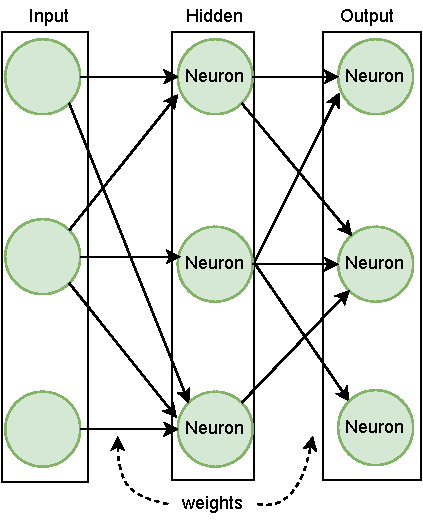
\includegraphics[width=0.2\textwidth]{simpleFFNN}
		\label{fig:simpleNN}}
	\hfil
	\subfloat[]
	{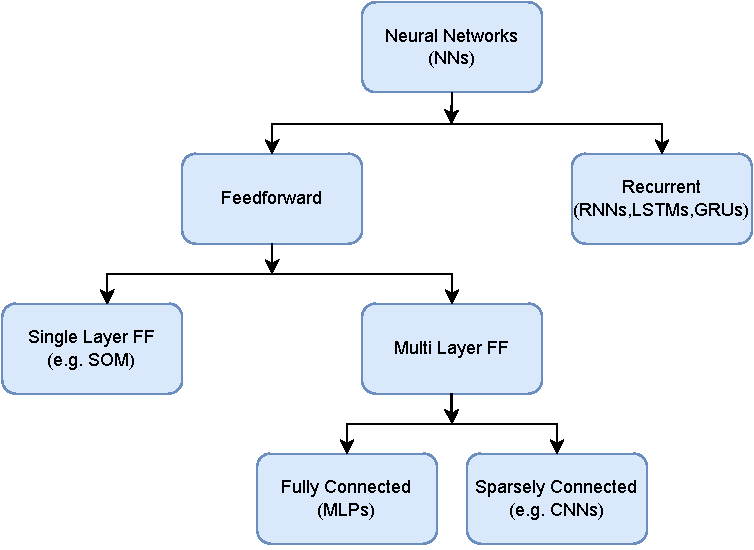
\includegraphics[width=0.5\textwidth]{nnClassification}
		\label{fig:nnClassification}}
	\hfil
	\caption{(a) Example of simple Neural Network. (b) Broad categories of NNs.}
	\label{fig:intro}
\end{figure}
\subsection{Broad Classification}
There are several classes of NNs that differ from each other in the number of neurons, connections between them, and method of training. \figurename{~\ref{fig:nnClassification}} shows two broad classes of NNs, feedforward neural networks (FFNNs) and recurrent neural networks (RNNs). 

FFNNs approximate some function to map input to output using a set of parameters (weights and biases). In FFNNs, the data flows from the input layer to the output layer via intermediate layers a.k.a. hidden layers, and there are no feedback connections. These can be represented as directed acyclic graphs. FFNNs do not have any internal state, and output depends on the current input and the parameters. Based on the number of layers, FFNNs can be further classified as single-layer and multi-layer FFNNs. Single-layer Feedforward NNs consist of just two layers - an input and an output layer. Only the output layer performs computation. Self-Organizing Maps (SOMs) are examples of single-layer NNs and are used in dimensionality reduction and clustering applications. 

Multilayer FFNNs represent the most important class of machine learning algorithms. They are used in several commercial applications and are the stepping stone of several other kind of NNs. They consist of one or more intermediate layers (hidden layers) between the input and output layers. Depending on whether the neurons in the layer are connected to all or a few of the neurons in the previous layers, these can be further classified as fully connected FFNNs (\figurename{~\ref{fig:fullyConnected}}) or sparsely connected FFNNs (\figurename{~\ref{fig:sparselyConnected}}), respectively. One of the most popular class of FFNNs used for image classification and recognition from images is Convolutional Neural Networks (CNNs).

Another popular class of NNs is recurrent neural networks (RNNs), which have layers with loops (\figurename{~\ref{fig:recurrentLayer}}). These loops represent that the output at any step is influenced by the previously seen inputs. These networks extract information from the inputs and store it in an internal state. In this class of NNs, the output depends not only on the current input but also on the internal state. They share the weights across different time steps of the sequence. These networks are widely used in speech recognition, natural language processing (NLP), and other sequential data processing applications. Long short-term memory networks (LSTMs) are among the popular variants of RNNs.

\begin{figure}[!htb]
	\centering
	\captionsetup{font=sf}
	\subfloat[]
	{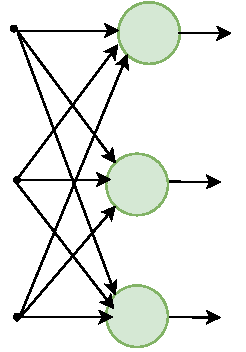
\includegraphics[width=0.15\textwidth]{fullyConnected}
		\label{fig:fullyConnected}}
	\hfil
	\subfloat[]
	{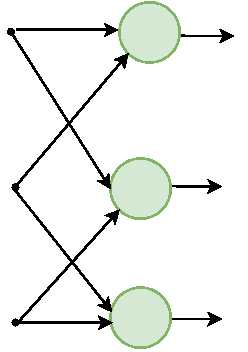
\includegraphics[width=0.15\linewidth]{sparselyConnected}
		\label{fig:sparselyConnected}}
	\hfil
	\subfloat[]
	{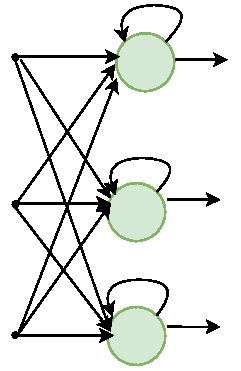
\includegraphics[width=0.15\linewidth]{recurrentLayer}
		\label{fig:recurrentLayer}}
	\caption{Types of NN layers (a) Fully Connected FF. (b) Sparsely Connected FF. (c) Recurrent. }
	\label{fig:nnLayers}
\end{figure}
Multilayer NNs with more than three layers are referred to as deep neural networks (DNNs), capable of learning complex functions. 
\subsection{Training Vs. Inference}
NNs are machine learning algorithms and need not be programmed explicitly. They learn from the raw data to provide solutions to real world problems. For example, to classify the class of an object in an image or to identify the speaker's age, sex from a voice sample. In this learning process they are provided a large set of real world examples and they determine the weights and biases of each neuron. This learning process is referred to as training of the neural network. Once trained the NN can estimate the output for a new set of inputs using the weights and biases learned during the training. Estimating the output for a new input using trained weights and biases is referred to as inference.

The objective of the training is to determine the weights and biases to achieve high accuracy. The accuracy is measured using a score value which estimates the difference between the expected and produced output by the NN. During the training a loss function is used to determine the correctness of the output. Using this loss function, weights are updated using some optimization technique, generally gradient descent. The gradient descent involve computations of partial derivatives to estimate the loss due to each weight by using chain rule of calculas. This involves storing the intermediate output of the network and thus require large storage. During the training, computations are performed using high precision to avoid accuracy loss, which further increases the storage and computations requirements.

Recently, DNN models with several hundreds of layers have been reported~\cite{he2016deep}. These DNNs have millions of parameters (weights and biases). For learning, these DNNs require large training data sets, and need to go through multiple iterations to achieve the desired accuracy, requiring significant computational resources and time. 

\figurename{~\ref{fig:workFlow}} shows difference phases of NNs. The development phase, which is usually performed on desktop/laptop machine. To speed up the development there are several popular NN frameworks e.g., PyTorch, TensorFlow etc. These framework implements layers commonly used in NNs, loss functions, backpropogation etc. They also support  methods to estimate and visualize the accuracy of the NNs, access to freely available training and testing data sets. 
\begin{figure}[!htb]
	\centering
	\captionsetup{font=sf}
	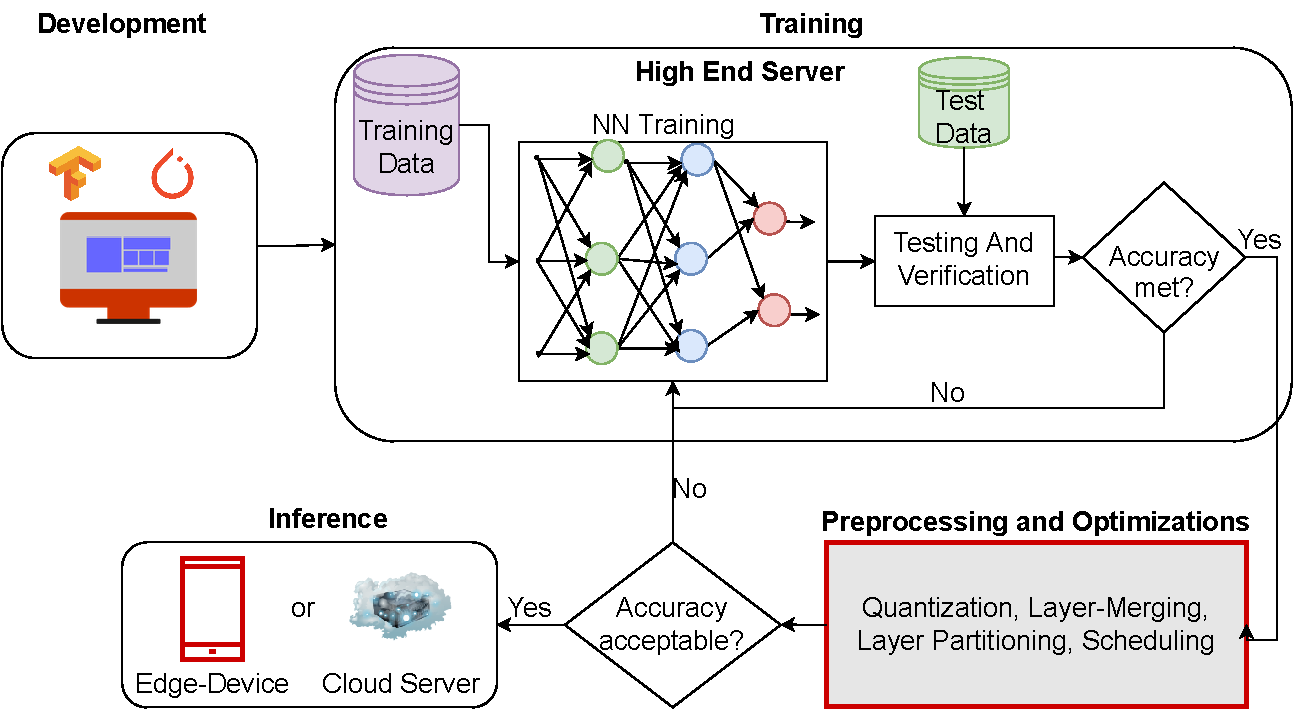
\includegraphics[width=0.7\textwidth]{WorkFlow}
	\caption{Work Flow for Neural Networks.}
	\label{fig:workFlow}
\end{figure}

Training of NNs involve updating weights and biases using large number of input samples. Its a repetitive process, until the desired accuracy is achieved. Training a DNN may last from few hours to several weeks. Hence training of DNNs are generally performed on high performance systems typically using GPUs. NN frameworks provide ways to save the trained model weights and biases which are used in optimization and inference phase. Once these models are trained, they can be deployed in applications for inferencing, where the deployment platforms may range from cloud to embedded devices. 

\begin{figure}[!htb]
	\centering
	\captionsetup{font=sf}
	\subfloat[]
	{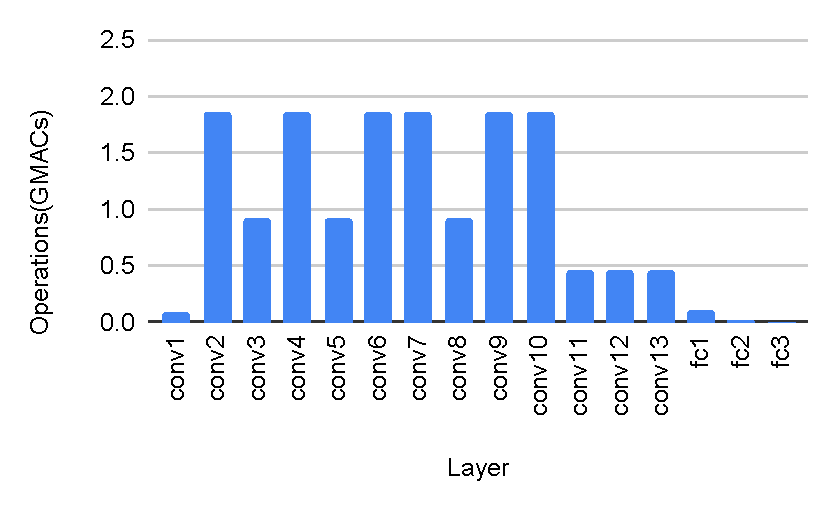
\includegraphics[width=0.45\textwidth]{vgg16GMACsOverview}
		\label{fig:vgg16GMACsOverview}}
	\hfil
	\subfloat[]
	{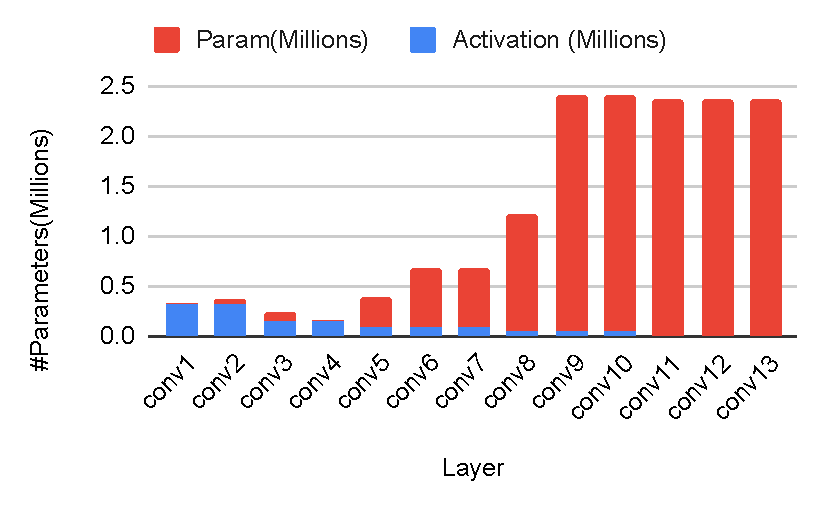
\includegraphics[width=0.45\linewidth]{vgg16ParamsOverview}
		\label{fig:vgg16ParamsOverview}}
	\caption{VGG16: A Convolution NN (a) Multiply And Accumlate Operations (MACs) per Inference. (b) Number of Parameters used per Inference.}
	\label{fig:MACAndParamsSize}
\end{figure}
\figurename{~\ref{fig:vgg16GMACsOverview}} and \figurename{~\ref{fig:vgg16ParamsOverview}} shows the layer wise distribution of number of operations (MACs) and parameters accessed per inference in a popular Convolution NN, VGG16, respectively. Overall for a single inference, VGG16 performs 15.47 GMACs operations and accesses 138 million parameters. This illustrates, inferencing involve compute and memory intensive operations. If the NNs are deployed on the cloud, the throughput and energy demands can be met using high performance systems like GPU. However, on edge devices, which have limited resources and tight energy budged, it is a challenge. Hence optimizing these models before inferencing on edge devices is a must. In this work we mainly focus on optimizing NN models before they are used for inference in energy constrained edge-devices.

\section{Edge AI}
Few years back, inferencing were commonly performed on the cloud, while the edge devices were used for collecting the real world data. Recent growth of deep learning has enabled several intelligent applications for consumer and edge devices. Today we see explosion of applications using deep learning algorithms in consumer electronic devices. Advancement in deep learning tools, and recent researches in the field of edge AI accelerators are the key enablers of edge AI. Deep learning tools that were earlier used by researchers, have evolved in past few years and now even non-experts can use them to develop intelligent applications. Recent research to improve the computation and energy efficiency of Edge AI accelerators also enabled this transition. 

Edge AI is gaining momentum as it improves the user experience, eliminates network bandwidth issues, and improves privacy and security. Due to these reasons, there is a growing trend of shifting the processing of these DNN applications from cloud to edge devices, near the sensors. Manufacturers are shifting the processing of NNs from cloud to edge devices like smartphones and tablets. 

Edge AI devices are battery-operated with limited resources and a tight energy budget which poses significant challenges in processing NNs inference. \figurename{~\ref{fig:edgeAIChallenges}} shows the key challenges for Edge AI devices. Energy efficiency and throughput are the two most important metrics for edge devices. While energy efficiency is of paramount importance for longer battery time, high throughput is desired for better user-response time. Efficient processing of DNNs inferencing on edge devices is critical for their widespread usage. 
\begin{figure}[!htb]
	\centering
	\captionsetup{font=sf}
	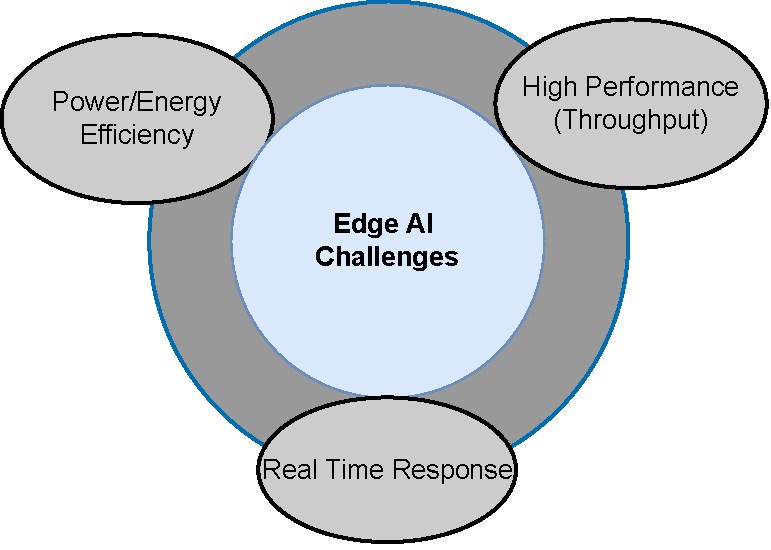
\includegraphics[width=0.6\textwidth]{edgeAIChallenges}
	\caption{Key challenges for Edge-AI Accelerator}
	\label{fig:edgeAIChallenges}
\end{figure}
\section{Customized NN Accelerator}
Edge devices mostly use customized accelerators to meet energy and throughput demands. Several FPGA~\cite{zhang2015optimizing,wei2019overcoming,gokhale2014240,8742284,gupta2015deep,alwani2016fused}, GPU~\cite{chetlur2014cudnn} and ASIC~\cite{Chen2016EyerissAS,chen2014diannao,chen2014dadiannao,du2015shidiannao} accelerators have been proposed to meet the performance and energy targets. 

\figurename{~\ref{fig:typicalDNNAccelerator}} shows a typical DNN accelerator architecture, which consists of an off-chip memory and an accelerator chip. An accelerator chip mainly consists of an on-chip memory of a few hundred KBs and an array of Processing Elements (PEs). The accelerator system has multiple memory levels: off-chip memory, on-chip memory, and the registers inside the PEs. As shown in \figurename{~\ref{fig:memoryHierarchy}}, each memory level has different storage capacity, access latency and energy costs. The memory access energy from off-chip memory is up to two orders of magnitude higher than a PE computation operation~\cite{Chen2016EyerissAS}. 
\begin{figure}[!htb]
	\centering
	\captionsetup{font=sf}
	\subfloat[]
	{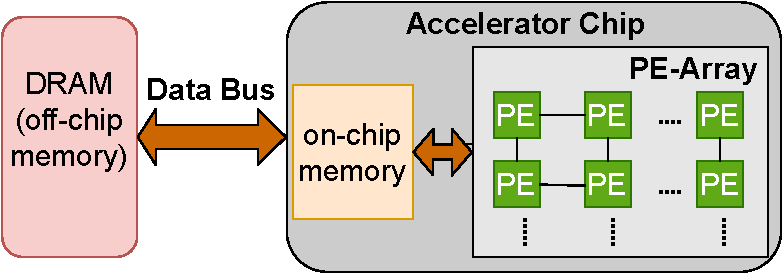
\includegraphics[width=0.5\textwidth]{typicalDNNAccelerator}
		\label{fig:typicalDNNAccelerator}}
	\hfil
	\subfloat[]{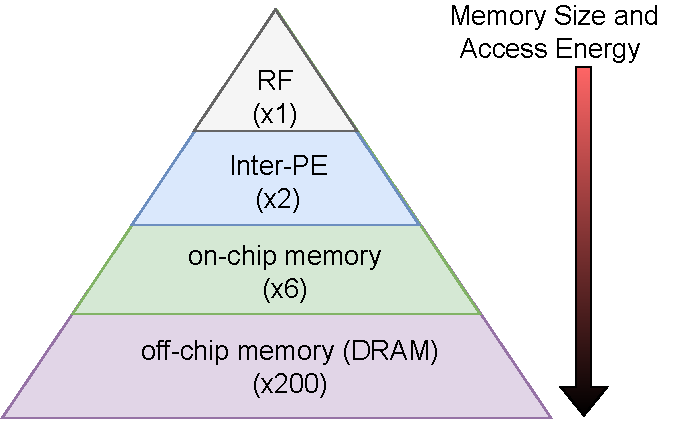
\includegraphics[width=0.4\textwidth]{memoryLevelsEnergy.pdf}
		\label{fig:memoryHierarchy}}
	\caption{(a) Typical DNN accelerator architecture. (b) Memory access energy consumption, normalized w.r.t. MAC Operation.}
	\label{fig:acceleratorAndRoofline}
\end{figure}

\figurename{~\ref{fig:energyDistribution}} shows the energy consumption of NN accelerator results from computations ($E_{comp}$) and data movement ($E_{data}$). The number and type of operations in NN layers are known. $E_{data}$ can be computed by accumlating the products of energy per operation and number of operations for different type of operations involved in the layer. $E_{data}$ can be estimated by multiplying number of memory accesses and energy per access for a given memory. NN accelerator has multiple levels of memory and and the number of memory accesses at each level depends on the data flow scheme used, type of layer, etc., which makes estimating $E_{data}$ challenging . $E_{data}$ is a sum of data access energy from the off-chip memory $E_{OffChip}$ and on-chip memory $E_{OnChip}$. Multiple levels of memories inside the accelerator chip contribute to $E_{OnChip}$ as shown in \figurename{~\ref{fig:energyDistribution}}. It has been observed that more than 80\% of the overall energy consumption of these accelerators is due to off-chip memory accesses ($E_{OffChip}$) ~\cite{chen2014diannao}. 
\begin{figure}[!htb]
	\centering
	\captionsetup{font=sf}
	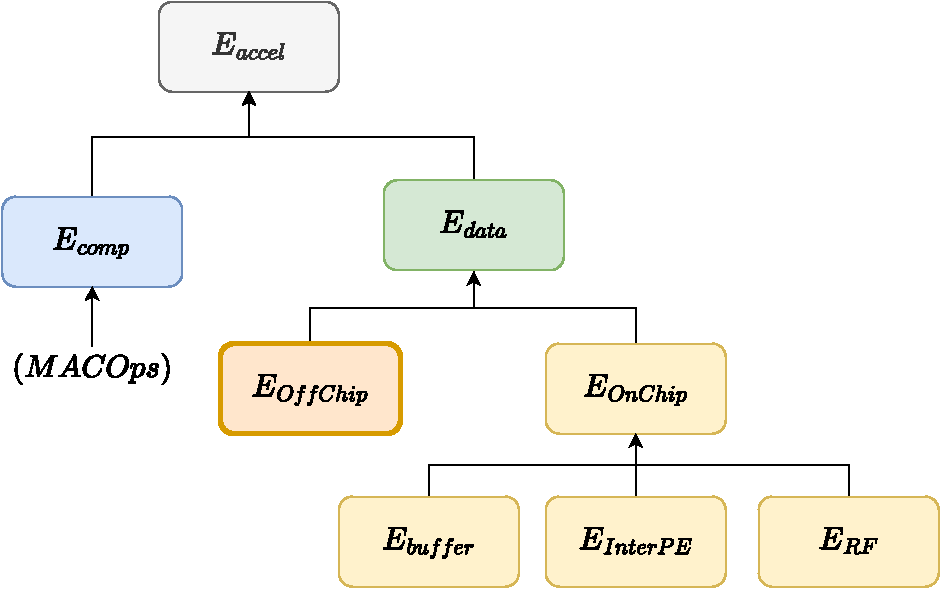
\includegraphics[width=0.6\textwidth]{energyTriangle.pdf}
	\caption{Computation and data movement energy in NN accelerators.}
	\label{fig:energyDistribution}
\end{figure}

\begin{figure}[!htb]
	\centering
	\captionsetup{font=sf}
	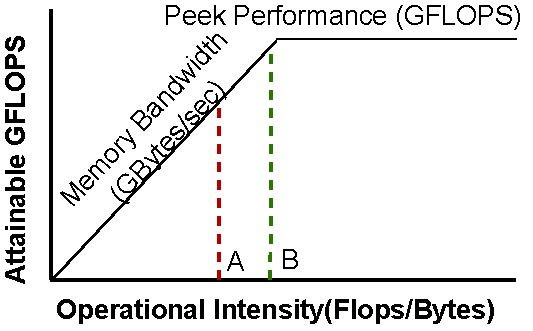
\includegraphics[width=0.4\linewidth]{roofline}
	\caption{Roofline Model}
	\label{fig:roofline}
\end{figure}

The PE-array (\figurename{~\ref{fig:typicalDNNAccelerator}}) has a large number of processing elements, capable of performing several operations per cycle. However, throughput is often limited by off-chip memory bandwidth~\cite{williams2009roofline}. Fig.~\ref{fig:roofline} shows attainable throughput in such a scenario as a function of the operational intensity of an application. The figure shows two application kernels (A and B) with different operational intensities (FLOPS/byte), with performance limited by the memory bandwidth in both cases, which is typically the case for most DNN accelerators. Kernel B, however, has better operational intensity than kernel A and achieves better throughput. Effective data-reuse techniques are required to improve the performance of bandwidth-limited parallel architectures. Therefore, reducing the off-chip memory is the key to improving the throughput and energy efficiency of DNN accelerators. Most recent research has focused on reducing off-chip memory accesses.
\section{Efficient Processing of NNs}
\begin{figure}[!htb]
	\centering
	\captionsetup{font=sf}
	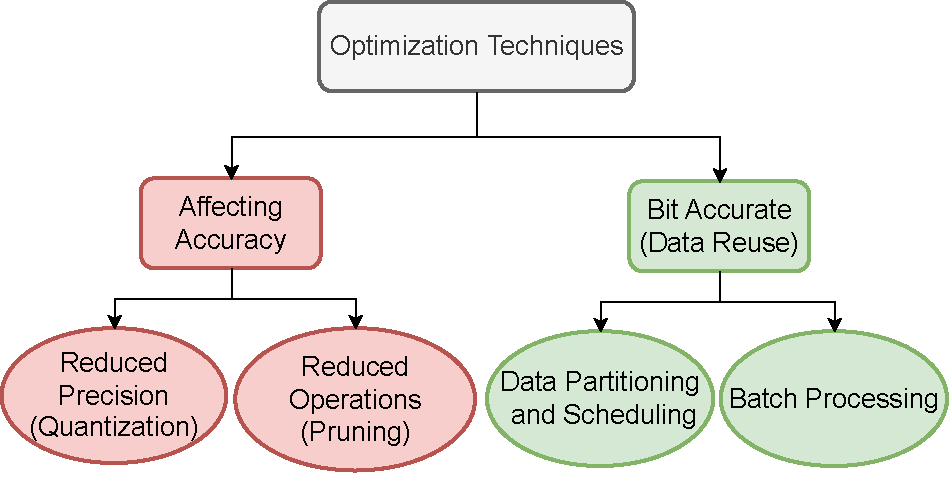
\includegraphics[width=0.5\textwidth]{previousWorkClassification}
	\caption{Broad Classification of previous works for improving the performance of DNN accelerators.}
	\label{fig:previousWorkClassification}
\end{figure}
Recent works that aim to reduce the off-chip memory accesses of NN accelerators can be classified into two broad categories, as shown in Figure~\ref{fig:previousWorkClassification}. One category of work exploits error-tolerance and redundancy in NNs using quantization, compression, and pruning techniques to reduce the precision, the number of operations and models' size~\cite{ferreira2016fpga,wang2018c,chang2015recurrent,han2017ese,lee2016fpga}. With reduced precision, the storage requirement and memory accesses reduce proportionally and improve energy efficiency~\cite{sze2017efficient}. In shallow NNs, the number of parameters is smaller compared to DNNs. Quantization and pruning techniques result in reduced NN model sizes. The reduced model for shallow NNs may fit into the on-chip memory and thus eliminate the off-chip memory bandwidth bottleneck. However, quantization and pruning approaches impact the accuracy of the networks and may not be suitable where accuracy can not be compromised. Also, the number of parameters in modern DNNs is significantly large. For these DNNs, besides quantization and pruning, additional techniques are required to further reduce the off-chip memory accesses.

The other approach, which does not affect the accuracy of the network, is to reduce repeated off-chip accesses to the same NN coefficients when the entire set of NN coefficients does not fit in the on-chip memory. This is quite effective for many modern DNNs (e.g., CNNs, RNNs) with a significantly large number of parameters~\cite{zhang2015optimizing,Li2018SmartShuttleOO,que2019efficient,park2020time}. The weights are repeatedly used for all the inputs during the inference phase. Inputs can be grouped as a batch and processed to reuse the weights. This technique is referred to as batch processing. Increasing the batch size increases the weights reuse but also increases the latency. Another prominent data reuse technique is data partitioning and scheduling. In this technique, the data is partitioned into tiles, and operations on tiles are scheduled in such a way that data can be accessed from the on-chip memory, as far as possible. For a given DNN, there are numerous ways of doing data partitioning and scheduling, offering different extents of data reuse. Choosing an optimal way here is non-trivial.

The data-reuse approaches are orthogonal to the quantization techniques and can be combined to reduce the off-chip memory accesses further. In this work, we have explored both types of approaches and contributed some new ideas.

\section{Summary and Outline of the Thesis} 
Recent advancement in NNs have enabled them to solve several real world problems which long ago was dreamed by the researchers. Due to their high accuracy they are now being used in wide range of domains. Last few years have witnessed the enormous growth in number of intelligent applications targeted for edge devices. However, resource and energy constrained on edge device poses a significant challenge for the wide acceptance of NN applications. Hence there is a pressing need for energy efficient execution of NNs applications. In NN inference phase, large amount of energy consumptions results from expensive off-chip memory accesses. A key to improve the performance and energy efficiency of these edge devices is to optimize the memory accesses.
 
Previous research has shown that for data partitioning and scheduling, making a choice independently for each layer of a NN is better than making a common choice for the entire NN because of the different shapes of various layers. We observe that the choice of optimal data partitioning and scheduling not only depends on the shape of a layer but also on some architectural parameters. We present an analytical framework in Chapter 2 that quantifies the off-chip memory accesses and compute cycles for DNN layers of varying shapes, also taking into account the architectural constraints. It is useful for comparing different data partitioning and scheduling schemes to explore the large design space in order to find the optimal solution for improving the energy and throughput. 

Based on the above analytical framework, in Chapter 3 we propose a data reuse approach that takes into account the architectural parameters and determines the optimal partitioning and scheduling scheme to minimize the off-chip memory access of DNN layers. We demonstrate the efficacy of our partitioning and adaptive scheduling approach on the compute and memory-intensive CNN layers. 

In Chapter 4, we propose a novel data reuse approach to improve the throughput and energy efficiency of state-of-the-art recurrent neural networks (RNNs). The proposed approach splits the computations and combines them in a way that reduces the off-chip memory accesses of large matrices significantly. We measure the design power and memory accesses on FPGA implementation of Long-Short Term Memory Network (LSTM) accelerators and show the energy and throughput improvements achieved by our approach.
	
We analyze the effect of using different bit resolutions on the accuracy of a NN, as well as the benefits of using low bit-width data resolution for self organizing maps (SOMs) for designing energy-constrained systems where the area, power, and performance are of critical importance in Chapter 5. Using an efficient implementation of SOM design on FPGA, which can be configured for different bit resolutions, we show performance comparison for different data precisions. 
	
The work done in this thesis not only improves the state-of-the-art for energy efficient execution of modern NNs, but also gives directions to future research. In chapter 6, we discuss these new research directions together with the conclusion of our work.
%%\documentclass[11pt,twoside,a4paper]{report}
\documentclass[12pt,twoside]{book}
\pdfminorversion=1

\setcounter{secnumdepth}{4}

%\usepackage{amsthm}
\usepackage{xspace}
%\usepackage{myalgorithm}
%\usepackage{myalgorithmic}
\usepackage{algorithm, algorithmicx}
\usepackage[noend]{algpseudocode}
\usepackage{tabu}
\usepackage{bbm}
\usepackage{caption}
\usepackage{verbatim}
\usepackage{comment}
\usepackage{epsfig} 
\usepackage{xcolor}
%\usepackage{subfigure}
\usepackage[figuresright]{rotating}
\usepackage{makeidx}
\usepackage[nottoc,notlof,notlot]{tocbibind}
\usepackage{setspace}
\usepackage{latexsym,amssymb,amsmath,bm}
\usepackage{bbm}
\usepackage{amsthm}
\usepackage{threeparttable}
\usepackage{colortbl}

%\usepackage[standard]{ntheorem}
\newtheorem{axiom}{Axiom}
\DeclareMathOperator{\Exists}{\exists}
\DeclareMathOperator{\Forall}{\forall}

\usepackage{makeidx}
\usepackage{lscape}
\usepackage{verbatim}
\usepackage{rotate}
\usepackage{placeins}
\usepackage{fancyvrb}

\usepackage{amsmath}
%\usepackage{mathptmx}
\usepackage{helvet}
\usepackage{courier}
\usepackage{type1cm}         
\usepackage{graphicx}        % standard LaTeX graphics tool
\usepackage{multicol}        % used for the two-column index
\usepackage[bottom,stable]{footmisc}% places footnotes at page bottom
\usepackage{fancyhdr}
\usepackage[english]{babel}
\makeatletter\AtBeginDocument{\let\@elt\relax}\makeatother %fix by Saurabh for compiling tex
\usepackage{multirow}
\usepackage{longtable,booktabs,makecell}

\usepackage{enumerate}
\usepackage{times}
\usepackage{moreverb} 
\usepackage{listings}
\usepackage{xcolor}			

\usepackage{rotating}
\usepackage{multicol}
\usepackage{fancybox}
\usepackage{textcomp}
\usepackage{pdfpages}
%\usepackage{named}
\usepackage[numbers,sort]{natbib}
%\usepackage{hyperref}
%\usepackage{subfig}
\usepackage{xcolor}


 \usepackage{subcaption}

% \usepackage{cleveref}

% \captionsetup[subfigure]{subrefformat=simple,labelformat=simple}
% \renewcommand\thesubfigure{(\alph{subfigure})}

\usepackage{float}
\floatstyle{ruled}

\usepackage[hyphens]{url}
\usepackage[pdfpagemode={UseOutlines},bookmarks=true,bookmarksopen=true,
   pdfauthor={Saurabh Tewari},pdfcreator={Saurabh Tewari},
   bookmarksopenlevel=0,bookmarksnumbered=true,hypertexnames=false,
   colorlinks,linkcolor={black},citecolor={black},urlcolor={black},
   pdfstartview={FitV},unicode,breaklinks=true]{hyperref}
\def\figref#1{Figure~\ref{#1}}
\def\eqref#1{Equation~\ref{#1}}
\def\chapref#1{Chapter~\ref{#1}}
\def\secref#1{Section~\ref{#1}}
\def\appref#1{Appendix~\ref{#1}}
\def\eqnref#1{Equation~(\ref{#1})}
\def\tabref#1{Table~\ref{#1}}
\def\algref#1{Algorithm~\ref{#1}}

%\hyphenation{Balakrishnan}

\newcommand{\subgraphname}{part}
\newcommand{\subgraphnamespace}{part }
\newcommand{\subgraphnameCaps}{Part}

\usepackage{mathtools}
\DeclarePairedDelimiter{\ceil}{\lceil}{\rceil}
\DeclarePairedDelimiter\floor{\lfloor}{\rfloor}
\newcommand{\numBytesOffChip}{\mathbb{B}}
\newcommand{\numOverlap}{\delta}
\newcommand{\busWidth}{BW}
\newcommand{\dataWidth}{DW}
\newcommand{\dataLength}{l}
\newcommand{\addressSym}{Addr}
\newcommand{\BuffSize}{buffSize}
\newcommand{\removelatexerror}{\let\@latex@error\@gobble}
%\input{defines}

\addtolength{\topmargin}{-45pt} %we cannot put this restriction
% \addtolength{\oddsidemargin}{10pt}
% \addtolength{\evensidemargin}{-65pt}
\addtolength{\evensidemargin}{-45pt}
\addtolength{\textwidth}{64pt}
\addtolength{\textheight}{90pt} %we cannot put this restriction
\setlength{\emergencystretch}{10pt}
%-------------------------------------------------------------------------
%\let\oldmarginpar\marginpar
%\renewcommand\marginpar[1]{\-\oldmarginpar[\raggedleft\small\itshape
%#1]{\raggedright\small\itshape #1}}
%------------------------------------------------------------------------- 


%customizing header
\pagestyle{fancy}
\renewcommand{\chaptermark}[1]{\markboth{#1}{}}
\fancyhf{}
\fancyhead[LO,RE]{\bfseries \leftmark}
\fancyhead[LE,RO]{\bfseries \thepage}
\fancyhead[RE]{\bfseries\leftmark}
\addtolength{\headheight}{14.6pt}

%change
%\renewcommand{\algorithmicrequire}{\textbf{Input:}}
%\renewcommand{\algorithmicensure}{\textbf{Output:}}


\let\mysubsection=\subsection % define a pointer to the current definition of the command \section
\renewcommand{\subsection}[1]{ \FloatBarrier\mysubsection{#1}}

\let\mysection=\section % define a pointer to the current definition of the command \section
\renewcommand{\section}[1]{ \FloatBarrier\mysection{#1}}



\newcommand{\etal}{\mbox{\it et al.}}

%\newtheorem{defn}{Definition}[section]
%\newtheorem{thm}{Theorem}[section]
%\newtheorem{lem}{Lemma}[section]

%\DeclareMathOperator*{\argmax}{arg\,max}
%\DeclareMathOperator*{\argmin}{arg\,min}

\definecolor{LightGray}{gray}{0.75}
\definecolor{DarkGray}{gray}{0.5}

\definecolor{dkgreen}{rgb}{0,0.6,0}
\definecolor{gray}{rgb}{0.5,0.5,0.5}
\definecolor{mauve}{rgb}{0.58,0,0.82}

% \lstset{frame=tb,
%   language=Java,
%   aboveskip=3mm,
%   belowskip=3mm,
%   showstringspaces=false,
%   columns=flexible,
%   basicstyle={\small\ttfamily},
%   numbers=none,
%   numberstyle=\tiny\color{gray},
%   keywordstyle=\color{blue},
%   commentstyle=\color{dkgreen},
%   stringstyle=\color{mauve},
%   breaklines=true,
%   breakatwhitespace=true
%   tabsize=3
% }

\definecolor{codegreen}{rgb}{0,0.6,0}
\definecolor{codegray}{rgb}{0.5,0.5,0.5}
\definecolor{codepurple}{rgb}{0.58,0,0.82}
\definecolor{backcolour}{rgb}{0.95,0.95,0.92}

\lstdefinestyle{mystyle}{
    backgroundcolor=\color{backcolour},   
    commentstyle=\color{codegreen},
    keywordstyle=\color{magenta},
    numberstyle=\tiny\color{codegray},
    stringstyle=\color{codepurple},
    basicstyle=\footnotesize,
    breakatwhitespace=false,         
    breaklines=true,                 
    captionpos=b,                    
    keepspaces=true,                 
    numbers=left,                    
    numbersep=5pt,                  
    showspaces=false,                
    showstringspaces=false,
    showtabs=false,                  
    tabsize=2
}
 
\lstset{style=mystyle}


\definecolor{Wheat3}{rgb}{0.803922,0.729412,0.588235}



%\algdef{SE}[DOWHILE]{Do}{doWhile}{\algorithmicdo}[1]{\algorithmicwhile\ #1}%

%\usepackage[linesnumbered,ruled,vlined]{algorithm2e} % For algorithms


\newtheorem{notation}{Notation}

\newcommand\mycommfont[1]{\footnotesize\ttfamily\textcolor{blue}{#1}}
%\SetCommentSty{mycommfont}
%\SetKwComment{Comment}{$\triangleright$\ }{}
\usepackage{enumitem}

%following four lines avoid hyphenation while still keeping the text within the margins
\tolerance=1
\emergencystretch=\maxdimen
\hyphenpenalty=10000
\hbadness=10000

\date{}
%\usepackage{layouts} %http://ctan.org/pkg/layouts
\begin{document}
%\pagevalues
%------------------------------------------------------------------------- 

%%%%%%%%%%%%%%%%%%%%%%%%%%%%%%%%%%%%%%%%%%%%%%%%%%%%%%%%%%%%%%%%%%%%%%%%%%
%%%%%%%%%%%%%%%%%%%%%%%%%%%%%%%%%%%%%%%%%%%%%%%%%%%%%%%%%%%%%%%%%%%%%%%%%%
%

%==================================================================================
%===          Switch on this part to generate Coverpage, Certificate, ACK
%==================================================================================

%\doublespacing
\pagestyle{empty}
%\cleardoublepage
%\newpage \ \newpage
\onehalfspacing 
%\newpage \ \newpage
%------------------------------------------------------------------------- 
\pagenumbering{gobble}
\begin{titlepage}

\begin{center}

%\vspace*{1cm}

\LARGE 

\MakeUppercase{\textbf{OPTIMIZING NEURAL NETWORKS PERFORMANCE ON PARALLEL ARCHITECTURES}}\\

\vspace{3cm}

\LARGE

\textbf{SAURABH TEWARI} 

%\vspace{8cm}
\vspace{6cm}
\hspace{0cm}
%\hbox{
\includegraphics[scale=1.0]{figures/logo.eps}}
%\hbox{
\includegraphics[width=8pc]{iitd-logo}}
\hbox{
\includegraphics[width=8pc]{ThesisSpecificPages/iitd-logo.pdf}}
\vspace{1cm}

\large{DEPARTMENT OF COMPUTER SCIENCE \& ENGINEERING}\\
\large{INDIAN INSTITUTE OF TECHNOLOGY DELHI}\\
\large{JULY 2023}\\

\end{center}

\end{titlepage}

% \cleardoublepage
% \begin{center}

\large

\ \\ \
\vspace{16cm}
\ \\ \
\copyright{ Saurabh Tewari, Indian Institute of Technology Delhi (IITD), 2023.}
\\ All rights reserved.

\end{center}


%\cleardoublepage
%\begin{titlepage}

\begin{center}


\LARGE
\MakeUppercase{\textbf{OPTIMIZING NEURAL NETWORKS PERFORMANCE ON PARALLEL ARCHITECTURES}}\\
\vspace{1cm}

\large

{by}\\
\vspace{.3cm}
{SAURABH TEWARI}\\
\vspace{.3cm}
{Department of Computer Science and Engineering}\\
\vspace{2cm}
{Submitted}\\
\vspace{0.3cm}
{in fulfillment of the requirements of the degree of Doctor of Philosophy}\\
\vspace{3cm}
{to the }\\
\vspace{1cm}
%\vspace{2.0cm}

\hspace{0cm}
\centering
\hbox{
\includegraphics[width=5pc]{ThesisSpecificPages/iitd-logo.pdf}}

\vspace{0.3cm}
{\bf
\large{INDIAN INSTITUTE OF TECHNOLOGY DELHI}\\
\large{JULY 2023}\\
}


\end{center}

%\end{titlepage}


%\cleardoublepage
\pagenumbering{roman}

%\newpage  \newpage
%\begin{center}
%	\ \\ \
%	\vspace{5.5cm}
%	\ \\ \
%	\large
%	DEDICATED TO\\
%	\textsf{\textit{\large{} My daughter Anika.}}
%	\par \end{center}{\large \par}

%\doublespacing 
%\chapter*{Certificate}
\phantomsection
\addcontentsline{toc}{chapter}{Certificate}
\begin{center}
	{\Huge \textbf{Certificate}} 
\end{center}

This is to certify that the thesis titled ``\textbf{OPTIMIZING NEURAL NETWORKS
	PERFORMANCE ON PARALLEL
	ARCHITECTURES}'' being submitted by  \textbf{Saurabh Tewari} for the award of \textbf{Doctor of Philosophy} in Computer Science and Engineering is a record of bonafide work carried out by him  under my guidance and supervision in the Department of Computer Science and Engineering, Indian Institute of Technology Delhi. The work presented in this thesis has not been submitted elsewhere, either in part or full, for the award of any other degree or diploma unless otherwise stated explicitly. 

Certain works included in this thesis involved collaboration or use of measurement data obtained by other students, which have been explicitly specified/acknowledged in the corresponding chapters and the part done by those collaborators appeared in their respective reports/theses.
%In particular, work done in Chapters 2 and 4 were done jointly with undergraduate students. In each case, the part done by the collaborators appeared in their respective Bachelor's theses.

\vspace {10 pc}

\begin{multicols}{2}
\noindent{\bf Anshul Kumar} \\
Professor \\
Department of Computer Science and Engg. \\
Indian Institute of Technology Delhi \\
New Delhi- 110016 \\
\columnbreak

\noindent{\bf Kolin Paul}\\
Professor \\
Department of Computer Science and Engg.\\
Indian Institute of Technology Delhi \\
New Delhi- 110016
\end{multicols}
\cleardoublepage

\pagestyle{plain}

%\doublespacing 
%%\addcontentsline{toc}{chapter}{Acknowledgements}
%\chapter*{Acknowledgements}
%\addcontentsline{toc}{chapter}{Acknowledgements}

%\addcontentsline{toc}{chapter}{\protect\numberline{}Acknowledgement}
%\setlength{\parindent}{0pt} 
%\setlength{\parskip}{2ex}

\phantomsection
\addcontentsline{toc}{chapter}{Acknowledgments}
\begin{center}
	{\Huge \textbf{Acknowledgments}} 
\end{center}

%\begin{flushright}
%{\em``{I can no other answer make but thanks, and thanks, and ever thanks.}"} \\ 
%	\vspace{0.20cm}
%\textemdash  \bf William Shakespeare, \em Twelfth Night
%\end{flushright}

\vspace{0.30cm}

I am deeply grateful to my esteemed Ph.D. supervisors, Prof. Anshul Kumar and Prof. Kolin Paul, for their exceptional guidance and unwavering support throughout my research journey. Their technical expertise and invaluable insights have been instrumental in shaping my academic growth and thesis work. They have not only provided mentorship but also offered valuable advice on various aspects of academic life, proving to be excellent mentors in every sense. Their constant availability for discussions, constructive suggestions, and motivation to complete my thesis on time have been indispensable. During the challenging times of the COVID-19 lockdown, their unwavering support kept me focused and encouraged.

Heartfelt appreciation goes to my research committee members, Prof. M. Balakrishnan and Prof. Preeti Ranjan Panda, for their valuable suggestions and feedback on my thesis work, enriching its quality and depth. I am also sincerely grateful to Prof. Ahmed Hemani, a professor at KTH Sweden, for offering me the opportunity to work in their state-of-the-art CGRA accelerator labs, significantly enhancing my research exposure and knowledge.

I extend my gratitude to all the instructors at IIT Delhi who imparted valuable skills during my coursework, contributing significantly to my overall academic growth.

Special thanks go to my friends at IIT Delhi, Rajesh Kedia, Sandeep Kumar, Dishant Goyal, and Omais Shafi, for their unwavering support and valuable suggestions on useful writing tools, aiding me in crafting research papers and creating graphical representations. In particular, I want to acknowledge Rajesh Kedia for his meticulous review and invaluable feedback. I am grateful to Vandana Ahluwalia, the lab incharge, for providing access to the labs and resources, and to Som Dutt Sharma from the DHD-LAB for granting access to the FPGA boards and essential software, which played a critical role in my research.

I am deeply thankful to my family members, including my wife, parents, and daughters, whose unwavering support and understanding made this achievement possible. Their love, encouragement, and sacrifices have been a constant source of motivation and strength. Lastly, I express gratitude to the Almighty for giving me the strength and opportunity to work with wonderful and helpful people.

I would also like to acknowledge all those whose names may not be mentioned here but have contributed in various ways, big or small, to my personal and academic growth. Their collective support and encouragement have been the driving force behind the successful completion of my Ph.D. thesis, and I humbly acknowledge their invaluable contributions.
\vspace{0.9cm}
{ \begin{flushright}{\bf Saurabh Tewari}\end{flushright} }

%\addcontentsline{toc}{chapter}{\numberline{}Acknowledgements}
%==================================================================================
%===
%==================================================================================

\normalfont

%==================================================================================
%=== Switch on this to generate TOC, ListOfFig, ListOfTab
%==================================================================================
%\singlespacing
\cleardoublepage
%\doublespacing 
\chapter*{Abstract}
\addcontentsline{toc}{chapter}{Abstract}
The recent past has observed explosive growth in the number of Neural Network (NN) based applications. Their ability to solve long outstanding problems with high accuracy has enabled new applications for consumer electronics and embedded devices. Their high accuracy comes at the cost of many computing and memory-intensive operations. A few years back, NN applications primarily ran on the cloud, but now they are preferred to run on the edge device to improve user experience. However, these edge devices’ limited computing and energy resources pose a significant challenge. Researchers have proposed several custom hardware accelerators to address these challenges. Throughput and energy consumption are the key performance metrics for these edge NN accelerators. These accelerators can meet the performance requirements to some extent, but their energy consumption is still concerning.

Energy-efficient processing of the NNs is paramount for their widespread usage on edge devices. A significant fraction of the energy consumption of these accelerators results from accessing the data from the off-chip memory accesses. The memory bandwidth also limits their throughput. Optimizing the off-chip memory accesses is the key to improving these accelerators' throughput and energy efficiency. This thesis focuses on energy-efficient inferencing of NNs on edge devices by optimizing the off-chip memory accesses at the pre-inferencing step.

Different NNs and layers of a NN exhibit different kinds of data access patterns. Data access patterns vary among the same type of layers within a NN due to varying layer shapes and sizes. There is no optimal global scheme that works for all. Off-chip memory accesses need to be analyzed for each case to find the optimal solution. Extracting the off-chip memory accesses directly from the NN description is difficult as it depends not only on the layer shape but also on the layer partitioning, scheduling, and accelerator's architectural parameters. This thesis proposes an analytical framework that computes the off-chip memory accesses for different types of NN layers and estimates the data movement energy. The analytical framework compares various design choices and trades between them. It guides for finding an energy-efficient solution for different NNs.

Different types of NNs are specialized for solving specific problems. These NNs differ in terms of the number of layers, parameters, data flow, training method, and type of operations. A few approaches can be applied for different NNs to reduce the off-chip memory accesses and works well for several NNs. For example, NNs are error tolerant, and thus representing data in low bit width can bring down energy consumption and storage requirements at the cost of some accuracy loss. However, more sophisticated optimization schemes specific to each NN are required to meet the energy targets. In this thesis, we have covered a range of NNs varying from single-layer, multi-layer feedforward NNs to recurrent NNs. 

To analyze the impact of low resolution on the accuracy of the NN and the benefits of it on energy consumption, we have applied this technique to Self Organizing Maps (SOM). SOM is an example of single-layer feedforward NN used in dimensionality reduction and clustering-related problems. We have implemented a custom pipelined FPGA design to accelerate the SOM processing. The target application is to identify bacterial genomes in clinical settings where optimizing energy and the area is critical. Using the FPGA design, we have analyzed the impact of varying data resolution on the accuracy of the network and energy and area benefits.

Convolution Neural Networks (CNNs) are multi-layer feedforward neural networks and have shown tremendous success in computer vision-related applications like object detection, image classification, and face detection. Loop tiling is commonly applied to partition the layer data into tiles. There are different ways in which layer data can be partitioned and the order in which operations on these tiles can be performed. Due to the large design space, finding the optimal solution is practically difficult by performing measurements on hardware. To address this, we have developed a model to compute the memory access of CLs and FCLs and integrated it with the analytical framework to analyze the memory accesses of different schemes. We have proposed a scheme to determine the optimal layer partitioning and scheduling scheme that maximizes the data reuse while considering the accelerator's architecture parameters, address alignment, and data resolution.

Recurrent Neural Networks (RNN) are another important category of NNs widely used for sequential data processing in speech recognition, natural language processing, and other areas. Long Short-Term Memory networks (LSTMs) are variants of RNNs, designed to handle long-range dependencies. RNNs have recurrent connections and internal states to store information from the past. Due to dependency on previous step computations, LSTM accelerators fail to reuse the data and incur a large volume of data accesses, resulting in high energy consumption. Memory bandwidth also limits the throughput of LSTM accelerators. In this work, we have proposed a novel data reuse scheme to overcome the data-dependency problem of LSTMs that significantly improves the data reuse and the throughput and energy consumption of these accelerators.

Overall, this thesis proposes an analytical framework to compute the memory accesses and analyze the data movement energy of state-of-the-art NNs and proposes novel data-reuse schemes to optimize the off-chip memory accesses of various NNs. This thesis contributes to the state-of-the-art by improving NN accelerators' energy efficiency and throughput during the inference phase.
\cleardoublepage
%\onehalfspacing 
%\includepdf[pages=-]{Hindi_Abstract.pdf}
\cleardoublepage
\setcounter{page}{7}
%\pagestyle{fancy}
\pagestyle{plain}
\tableofcontents

%\newpage \ \newpage
%\phantomsection
\listoffigures
\addcontentsline{toc}{chapter}{\listfigurename}
%\newpage \ \newpage

\listoftables
\addcontentsline{toc}{chapter}{List of Tables}
%\cleardoublepage
%\newpage
\newpage \ \newpage
\pagestyle{plain}
%==================================================================================
%=== After Activating Above you can deactivae bellow \TOC
%==================================================================================
%\tableofcontents
%\makeatletter\@addtoreset{chapter}{part}\makeatother%

\pagenumbering{arabic}
\pagestyle{plain}
\pagestyle{fancy}
%\singlespacing
%\onehalfspacing
%\doublespacing
%\part{Prologue}
\graphicspath{{./Ch1-Introduction/images/}}

\chapter{Introduction} \label{chap:introduction}
\begin{comment}
//clearly come out what are you doing in this thesis and what are the contributions
//what field you are targetting, scope and motivation, what problems, to justify your contributions.
1. About AI/ML/NN/DNNs: Applications, Domains, Growth, Type of NNs, Training and inference, 

2. Modern DNNs, architectures and popular NNs

3. Example: Number of computations, parameters: Illustrate compute and memory intensive operations.
Number of layer

4. Edge vs. Cloud Computing. 

5. Edge AI Challenges

6. About the Architectures for Edge AI Accelerators: Give wider scope of these architectures, and specific type of architectures. Trade-offs.

7. Performance bottlenecks for edge AI: Memory and Throughput bottlenecks.
Memory accesses are the key botllenecks for these edge AI devices. 

6. Summary and Outline of the Thesis.

\end{comment}

The past few years have seen exponential growth in Neural Network (NN) based applications. These are widely used in healthcare, agriculture, road safety, surveillance, defense, and others. Modern computing systems capable of storing and processing large volumes of data, and the availability of big data sets due to digitization, have enabled NNs to achieve human-like performance, which was not possible a few decades ago. Their growth was also accelerated by the software libraries like Tensorflow, PyTorch that provide ease of development. With time, NNs are growing in size to solve complicated problems and to improve the accuracy. 

\section{Neural Networks}
Machine learning is a field of Artificial Intelligence that give computers ability to learn from the data using training process without being programmed explicitly. Neural Networks are machine learning algorithms inspired by processing mechanisms in the human brain. Scientists believe that a human brain consists of several billions of computational units known as neurons. The computations of neurons involve weighted sum of input values known as activations. Inspired by the brain, NNs consist of several neurons connected and organized as layers. \figurename{~\ref{fig:simpleNN}} shows a simple NN example. Each layer has weights and biases, learned using the training process. The neurons in the input layer receives the input, performs the computations and passes the output to subsequent layer, known as hidden layer. There can be several hidden layers in a NN. The output of the final hidden layer is then passed to the output layer for the producing the result. 
\begin{figure}[!htb]
	\centering
	\captionsetup{font=sf}
	\subfloat[]
	{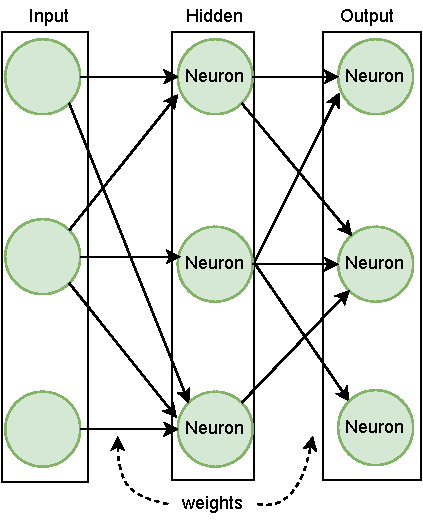
\includegraphics[width=0.2\textwidth]{simpleFFNN}
		\label{fig:simpleNN}}
	\hfil
	\subfloat[]
	{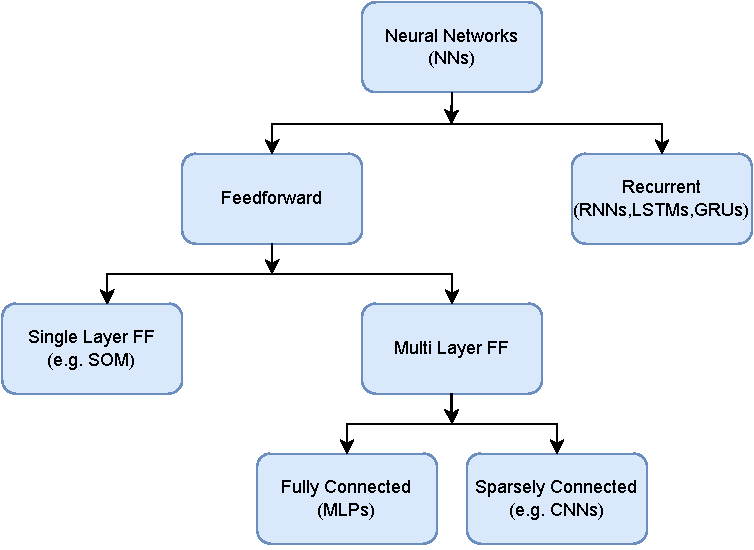
\includegraphics[width=0.5\textwidth]{nnClassification}
		\label{fig:nnClassification}}
	\hfil
	\caption{(a) Example of simple Neural Network. (b) Broad categories of NNs.}
	\label{fig:intro}
\end{figure}
\subsection{Broad Classification}
There are several classes of NNs that differ from each other in the number of neurons, connections between them, and method of training. \figurename{~\ref{fig:nnClassification}} shows two broad classes of NNs, feedforward neural networks (FFNNs) and recurrent neural networks (RNNs). 

FFNNs approximate some function to map input to output using a set of parameters (weights and biases). In FFNNs, the data flows from the input layer to the output layer via intermediate layers a.k.a. hidden layers, and there are no feedback connections. These can be represented as directed acyclic graphs. FFNNs do not have any internal state, and output depends on the current input and the parameters. Based on the number of layers, FFNNs can be further classified as single-layer and multi-layer FFNNs. Single-layer Feedforward NNs consist of just two layers - an input and an output layer. Only the output layer performs computation. Self-Organizing Maps (SOMs) are examples of single-layer NNs and are used in dimensionality reduction and clustering applications. 

Multilayer FFNNs represent the most important class of machine learning algorithms. They are used in several commercial applications and are the stepping stone of several other kind of NNs. They consist of one or more intermediate layers (hidden layers) between the input and output layers. Depending on whether the neurons in the layer are connected to all or a few of the neurons in the previous layers, these can be further classified as fully connected FFNNs (\figurename{~\ref{fig:fullyConnected}}) or sparsely connected FFNNs (\figurename{~\ref{fig:sparselyConnected}}), respectively. One of the most popular class of FFNNs used for image classification and recognition from images is Convolutional Neural Networks (CNNs).

Another popular class of NNs is recurrent neural networks (RNNs), which have layers with loops (\figurename{~\ref{fig:recurrentLayer}}). These loops represent that the output at any step is influenced by the previously seen inputs. These networks extract information from the inputs and store it in an internal state. In this class of NNs, the output depends not only on the current input but also on the internal state. They share the weights across different time steps of the sequence. These networks are widely used in speech recognition, natural language processing (NLP), and other sequential data processing applications. Long short-term memory networks (LSTMs) are among the popular variants of RNNs.

\begin{figure}[!htb]
	\centering
	\captionsetup{font=sf}
	\subfloat[]
	{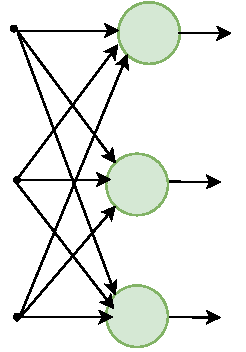
\includegraphics[width=0.15\textwidth]{fullyConnected}
		\label{fig:fullyConnected}}
	\hfil
	\subfloat[]
	{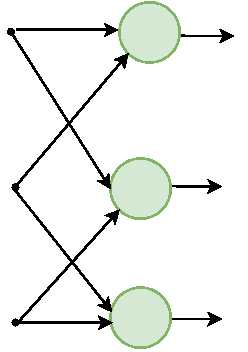
\includegraphics[width=0.15\linewidth]{sparselyConnected}
		\label{fig:sparselyConnected}}
	\hfil
	\subfloat[]
	{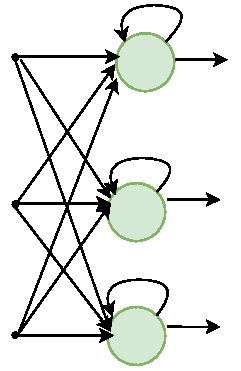
\includegraphics[width=0.15\linewidth]{recurrentLayer}
		\label{fig:recurrentLayer}}
	\caption{Types of NN layers (a) Fully Connected FF. (b) Sparsely Connected FF. (c) Recurrent. }
	\label{fig:nnLayers}
\end{figure}
Multilayer NNs with more than three layers are referred to as deep neural networks (DNNs), capable of learning complex functions. 
\subsection{Training Vs. Inference}
NNs are machine learning algorithms and need not be programmed explicitly. They learn from the raw data to provide solutions to real world problems. For example, to classify the class of an object in an image or to identify the speaker's age, sex from a voice sample. In this learning process they are provided a large set of real world examples and they determine the weights and biases of each neuron. This learning process is referred to as training of the neural network. Once trained the NN can estimate the output for a new set of inputs using the weights and biases learned during the training. Estimating the output for a new input using trained weights and biases is referred to as inference.

The objective of the training is to determine the weights and biases to achieve high accuracy. The accuracy is measured using a score value which estimates the difference between the expected and produced output by the NN. During the training a loss function is used to determine the correctness of the output. Using this loss function, weights are updated using some optimization technique, generally gradient descent. The gradient descent involve computations of partial derivatives to estimate the loss due to each weight by using chain rule of calculas. This involves storing the intermediate output of the network and thus require large storage. During the training, computations are performed using high precision to avoid accuracy loss, which further increases the storage and computations requirements.

Recently, DNN models with several hundreds of layers have been reported~\cite{he2016deep}. These DNNs have millions of parameters (weights and biases). For learning, these DNNs require large training data sets, and need to go through multiple iterations to achieve the desired accuracy, requiring significant computational resources and time. 

\figurename{~\ref{fig:workFlow}} shows difference phases of NNs. The development phase, which is usually performed on desktop/laptop machine. To speed up the development there are several popular NN frameworks e.g., PyTorch, TensorFlow etc. These framework implements layers commonly used in NNs, loss functions, backpropogation etc. They also support  methods to estimate and visualize the accuracy of the NNs, access to freely available training and testing data sets. 
\begin{figure}[!htb]
	\centering
	\captionsetup{font=sf}
	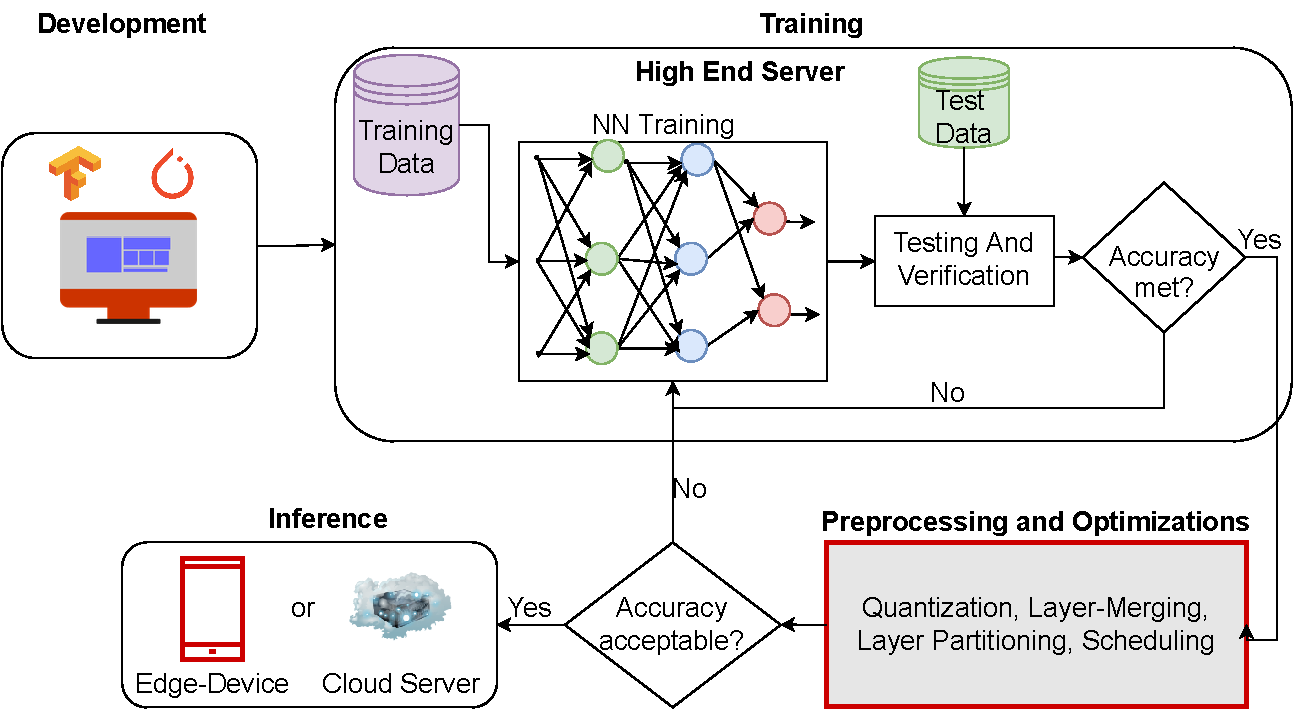
\includegraphics[width=0.7\textwidth]{WorkFlow}
	\caption{Work Flow for Neural Networks.}
	\label{fig:workFlow}
\end{figure}

Training of NNs involve updating weights and biases using large number of input samples. Its a repetitive process, until the desired accuracy is achieved. Training a DNN may last from few hours to several weeks. Hence training of DNNs are generally performed on high performance systems typically using GPUs. NN frameworks provide ways to save the trained model weights and biases which are used in optimization and inference phase. Once these models are trained, they can be deployed in applications for inferencing, where the deployment platforms may range from cloud to embedded devices. 

\begin{figure}[!htb]
	\centering
	\captionsetup{font=sf}
	\subfloat[]
	{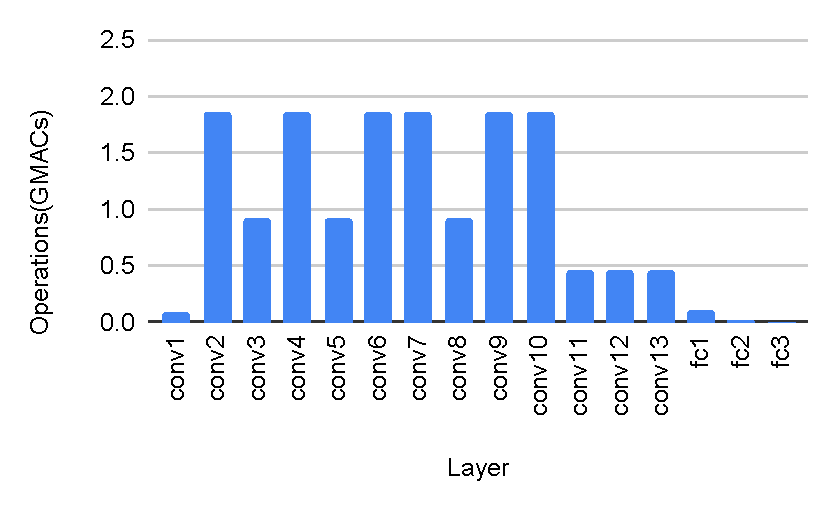
\includegraphics[width=0.45\textwidth]{vgg16GMACsOverview}
		\label{fig:vgg16GMACsOverview}}
	\hfil
	\subfloat[]
	{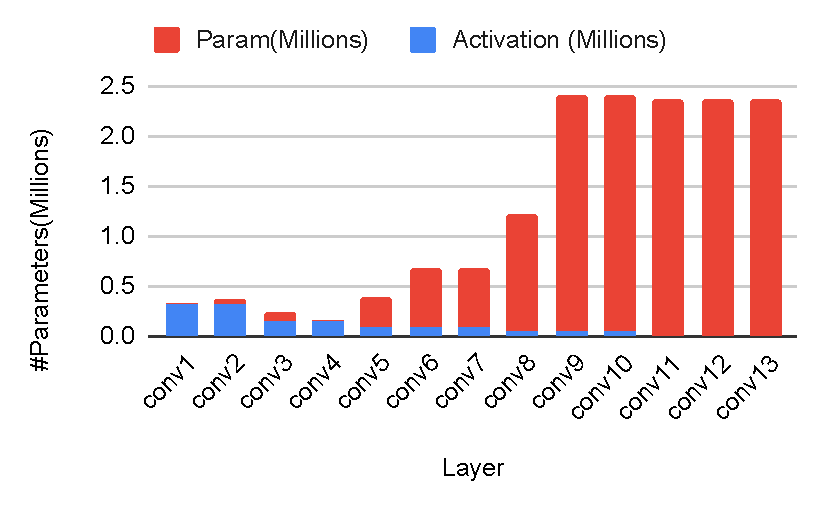
\includegraphics[width=0.45\linewidth]{vgg16ParamsOverview}
		\label{fig:vgg16ParamsOverview}}
	\caption{VGG16: A Convolution NN (a) Multiply And Accumlate Operations (MACs) per Inference. (b) Number of Parameters used per Inference.}
	\label{fig:MACAndParamsSize}
\end{figure}
\figurename{~\ref{fig:vgg16GMACsOverview}} and \figurename{~\ref{fig:vgg16ParamsOverview}} shows the layer wise distribution of number of operations (MACs) and parameters accessed per inference in a popular Convolution NN, VGG16, respectively. Overall for a single inference, VGG16 performs 15.47 GMACs operations and accesses 138 million parameters. This illustrates, inferencing involve compute and memory intensive operations. If the NNs are deployed on the cloud, the throughput and energy demands can be met using high performance systems like GPU. However, on edge devices, which have limited resources and tight energy budged, it is a challenge. Hence optimizing these models before inferencing on edge devices is a must. In this work we mainly focus on optimizing NN models before they are used for inference in energy constrained edge-devices.

\section{Edge AI}
Few years back, inferencing were commonly performed on the cloud, while the edge devices were used for collecting the real world data. Recent growth of deep learning has enabled several intelligent applications for consumer and edge devices. Today we see explosion of applications using deep learning algorithms in consumer electronic devices. Advancement in deep learning tools, and recent researches in the field of edge AI accelerators are the key enablers of edge AI. Deep learning tools that were earlier used by researchers, have evolved in past few years and now even non-experts can use them to develop intelligent applications. Recent research to improve the computation and energy efficiency of Edge AI accelerators also enabled this transition. 

Edge AI is gaining momentum as it improves the user experience, eliminates network bandwidth issues, and improves privacy and security. Due to these reasons, there is a growing trend of shifting the processing of these DNN applications from cloud to edge devices, near the sensors. Manufacturers are shifting the processing of NNs from cloud to edge devices like smartphones and tablets. 

Edge AI devices are battery-operated with limited resources and a tight energy budget which poses significant challenges in processing NNs inference. \figurename{~\ref{fig:edgeAIChallenges}} shows the key challenges for Edge AI devices. Energy efficiency and throughput are the two most important metrics for edge devices. While energy efficiency is of paramount importance for longer battery time, high throughput is desired for better user-response time. Efficient processing of DNNs inferencing on edge devices is critical for their widespread usage. 
\begin{figure}[!htb]
	\centering
	\captionsetup{font=sf}
	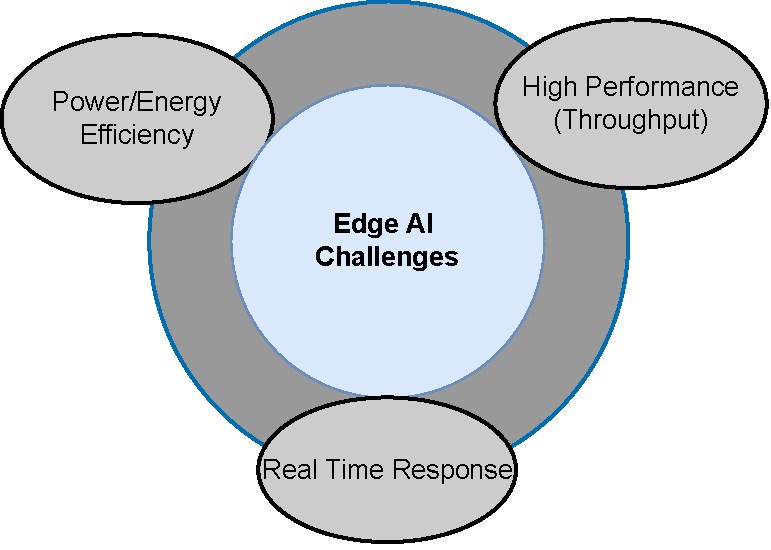
\includegraphics[width=0.6\textwidth]{edgeAIChallenges}
	\caption{Key challenges for Edge-AI Accelerator}
	\label{fig:edgeAIChallenges}
\end{figure}
\section{Customized NN Accelerator}
Edge devices mostly use customized accelerators to meet energy and throughput demands. Several FPGA~\cite{zhang2015optimizing,wei2019overcoming,gokhale2014240,8742284,gupta2015deep,alwani2016fused}, GPU~\cite{chetlur2014cudnn} and ASIC~\cite{Chen2016EyerissAS,chen2014diannao,chen2014dadiannao,du2015shidiannao} accelerators have been proposed to meet the performance and energy targets. 

\figurename{~\ref{fig:typicalDNNAccelerator}} shows a typical DNN accelerator architecture, which consists of an off-chip memory and an accelerator chip. An accelerator chip mainly consists of an on-chip memory of a few hundred KBs and an array of Processing Elements (PEs). The accelerator system has multiple memory levels: off-chip memory, on-chip memory, and the registers inside the PEs. As shown in \figurename{~\ref{fig:memoryHierarchy}}, each memory level has different storage capacity, access latency and energy costs. The memory access energy from off-chip memory is up to two orders of magnitude higher than a PE computation operation~\cite{Chen2016EyerissAS}. 
\begin{figure}[!htb]
	\centering
	\captionsetup{font=sf}
	\subfloat[]
	{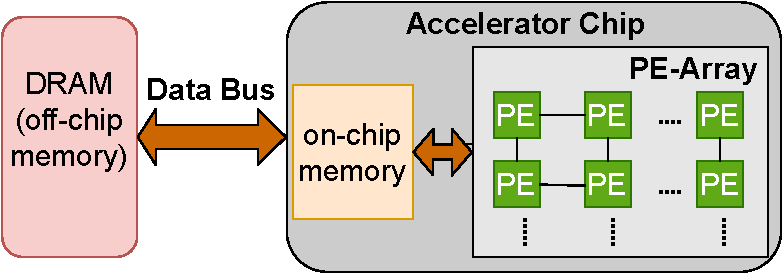
\includegraphics[width=0.5\textwidth]{typicalDNNAccelerator}
		\label{fig:typicalDNNAccelerator}}
	\hfil
	\subfloat[]{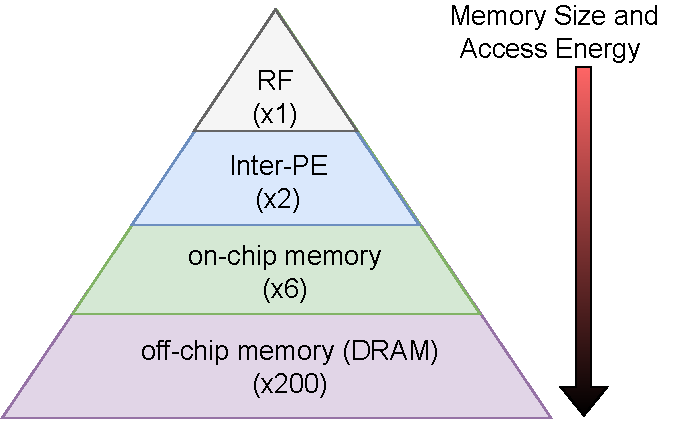
\includegraphics[width=0.4\textwidth]{memoryLevelsEnergy.pdf}
		\label{fig:memoryHierarchy}}
	\caption{(a) Typical DNN accelerator architecture. (b) Memory access energy consumption, normalized w.r.t. MAC Operation.}
	\label{fig:acceleratorAndRoofline}
\end{figure}

\figurename{~\ref{fig:energyDistribution}} shows the energy consumption of NN accelerator results from computations ($E_{comp}$) and data movement ($E_{data}$). The number and type of operations in NN layers are known. $E_{data}$ can be computed by accumlating the products of energy per operation and number of operations for different type of operations involved in the layer. $E_{data}$ can be estimated by multiplying number of memory accesses and energy per access for a given memory. NN accelerator has multiple levels of memory and and the number of memory accesses at each level depends on the data flow scheme used, type of layer, etc., which makes estimating $E_{data}$ challenging . $E_{data}$ is a sum of data access energy from the off-chip memory $E_{OffChip}$ and on-chip memory $E_{OnChip}$. Multiple levels of memories inside the accelerator chip contribute to $E_{OnChip}$ as shown in \figurename{~\ref{fig:energyDistribution}}. It has been observed that more than 80\% of the overall energy consumption of these accelerators is due to off-chip memory accesses ($E_{OffChip}$) ~\cite{chen2014diannao}. 
\begin{figure}[!htb]
	\centering
	\captionsetup{font=sf}
	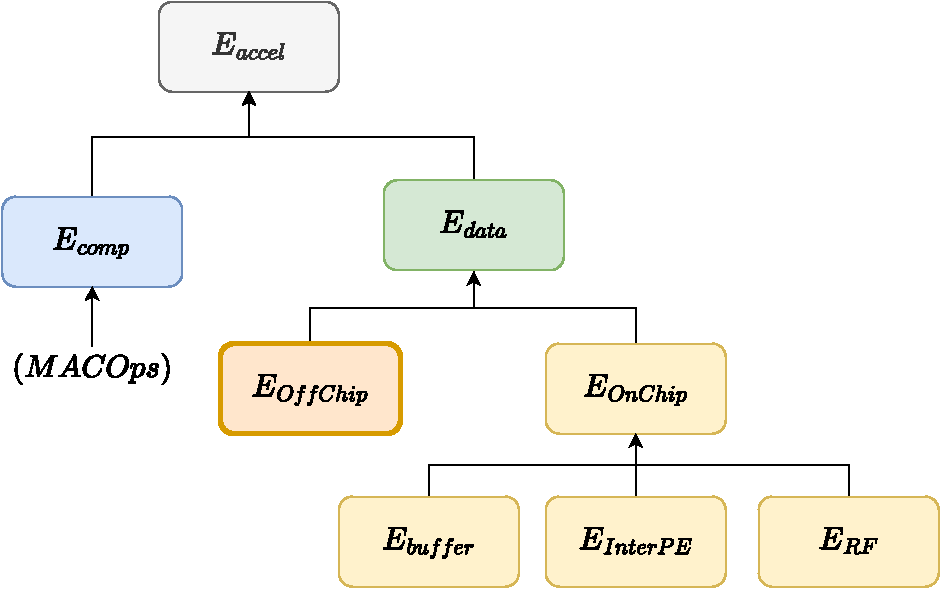
\includegraphics[width=0.6\textwidth]{energyTriangle.pdf}
	\caption{Computation and data movement energy in NN accelerators.}
	\label{fig:energyDistribution}
\end{figure}

\begin{figure}[!htb]
	\centering
	\captionsetup{font=sf}
	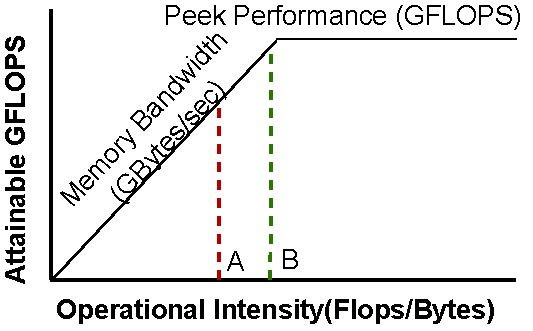
\includegraphics[width=0.4\linewidth]{roofline}
	\caption{Roofline Model}
	\label{fig:roofline}
\end{figure}

The PE-array (\figurename{~\ref{fig:typicalDNNAccelerator}}) has a large number of processing elements, capable of performing several operations per cycle. However, throughput is often limited by off-chip memory bandwidth~\cite{williams2009roofline}. Fig.~\ref{fig:roofline} shows attainable throughput in such a scenario as a function of the operational intensity of an application. The figure shows two application kernels (A and B) with different operational intensities (FLOPS/byte), with performance limited by the memory bandwidth in both cases, which is typically the case for most DNN accelerators. Kernel B, however, has better operational intensity than kernel A and achieves better throughput. Effective data-reuse techniques are required to improve the performance of bandwidth-limited parallel architectures. Therefore, reducing the off-chip memory is the key to improving the throughput and energy efficiency of DNN accelerators. Most recent research has focused on reducing off-chip memory accesses.
\section{Efficient Processing of NNs}
\begin{figure}[!htb]
	\centering
	\captionsetup{font=sf}
	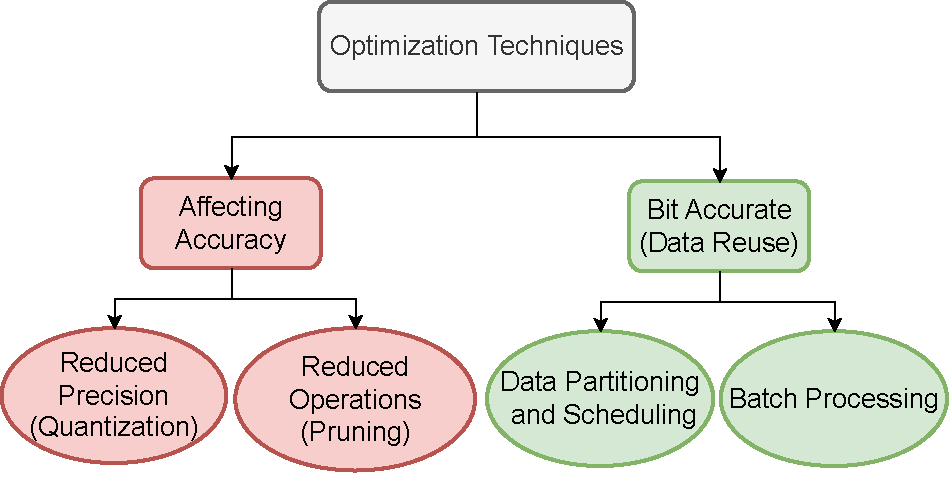
\includegraphics[width=0.5\textwidth]{previousWorkClassification}
	\caption{Broad Classification of previous works for improving the performance of DNN accelerators.}
	\label{fig:previousWorkClassification}
\end{figure}
Recent works that aim to reduce the off-chip memory accesses of NN accelerators can be classified into two broad categories, as shown in Figure~\ref{fig:previousWorkClassification}. One category of work exploits error-tolerance and redundancy in NNs using quantization, compression, and pruning techniques to reduce the precision, the number of operations and models' size~\cite{ferreira2016fpga,wang2018c,chang2015recurrent,han2017ese,lee2016fpga}. With reduced precision, the storage requirement and memory accesses reduce proportionally and improve energy efficiency~\cite{sze2017efficient}. In shallow NNs, the number of parameters is smaller compared to DNNs. Quantization and pruning techniques result in reduced NN model sizes. The reduced model for shallow NNs may fit into the on-chip memory and thus eliminate the off-chip memory bandwidth bottleneck. However, quantization and pruning approaches impact the accuracy of the networks and may not be suitable where accuracy can not be compromised. Also, the number of parameters in modern DNNs is significantly large. For these DNNs, besides quantization and pruning, additional techniques are required to further reduce the off-chip memory accesses.

The other approach, which does not affect the accuracy of the network, is to reduce repeated off-chip accesses to the same NN coefficients when the entire set of NN coefficients does not fit in the on-chip memory. This is quite effective for many modern DNNs (e.g., CNNs, RNNs) with a significantly large number of parameters~\cite{zhang2015optimizing,Li2018SmartShuttleOO,que2019efficient,park2020time}. The weights are repeatedly used for all the inputs during the inference phase. Inputs can be grouped as a batch and processed to reuse the weights. This technique is referred to as batch processing. Increasing the batch size increases the weights reuse but also increases the latency. Another prominent data reuse technique is data partitioning and scheduling. In this technique, the data is partitioned into tiles, and operations on tiles are scheduled in such a way that data can be accessed from the on-chip memory, as far as possible. For a given DNN, there are numerous ways of doing data partitioning and scheduling, offering different extents of data reuse. Choosing an optimal way here is non-trivial.

The data-reuse approaches are orthogonal to the quantization techniques and can be combined to reduce the off-chip memory accesses further. In this work, we have explored both types of approaches and contributed some new ideas.

\section{Summary and Outline of the Thesis} 
Recent advancement in NNs have enabled them to solve several real world problems which long ago was dreamed by the researchers. Due to their high accuracy they are now being used in wide range of domains. Last few years have witnessed the enormous growth in number of intelligent applications targeted for edge devices. However, resource and energy constrained on edge device poses a significant challenge for the wide acceptance of NN applications. Hence there is a pressing need for energy efficient execution of NNs applications. In NN inference phase, large amount of energy consumptions results from expensive off-chip memory accesses. A key to improve the performance and energy efficiency of these edge devices is to optimize the memory accesses.
 
Previous research has shown that for data partitioning and scheduling, making a choice independently for each layer of a NN is better than making a common choice for the entire NN because of the different shapes of various layers. We observe that the choice of optimal data partitioning and scheduling not only depends on the shape of a layer but also on some architectural parameters. We present an analytical framework in Chapter 2 that quantifies the off-chip memory accesses and compute cycles for DNN layers of varying shapes, also taking into account the architectural constraints. It is useful for comparing different data partitioning and scheduling schemes to explore the large design space in order to find the optimal solution for improving the energy and throughput. 

Based on the above analytical framework, in Chapter 3 we propose a data reuse approach that takes into account the architectural parameters and determines the optimal partitioning and scheduling scheme to minimize the off-chip memory access of DNN layers. We demonstrate the efficacy of our partitioning and adaptive scheduling approach on the compute and memory-intensive CNN layers. 

In Chapter 4, we propose a novel data reuse approach to improve the throughput and energy efficiency of state-of-the-art recurrent neural networks (RNNs). The proposed approach splits the computations and combines them in a way that reduces the off-chip memory accesses of large matrices significantly. We measure the design power and memory accesses on FPGA implementation of Long-Short Term Memory Network (LSTM) accelerators and show the energy and throughput improvements achieved by our approach.
	
We analyze the effect of using different bit resolutions on the accuracy of a NN, as well as the benefits of using low bit-width data resolution for self organizing maps (SOMs) for designing energy-constrained systems where the area, power, and performance are of critical importance in Chapter 5. Using an efficient implementation of SOM design on FPGA, which can be configured for different bit resolutions, we show performance comparison for different data precisions. 
	
The work done in this thesis not only improves the state-of-the-art for energy efficient execution of modern NNs, but also gives directions to future research. In chapter 6, we discuss these new research directions together with the conclusion of our work.
\graphicspath{{./Ch2-AnalyticalFw/images/}}

\chapter{Analyzing Off-chip Memory Accesses} \label{chap:analyticalFw}
The off-chip memory bandwidth often limits the performance of NN accelerators, and their high energy consumption also results from the large volume of off-chip memory accesses. NN accelerators use on-chip memories and reuse the data from it to minimize the number of off-chip memory accesses. Assuming that the data movement energy primarily depends on the number of bytes accessed from the memory, \figref{fig:memsAccess} illustrates the impact of data reuse from the on-chip memory on data movement energy. \figref{fig:memsAccessSingle} and \figref{fig:memsAccessDouble} show the number of memory accesses and energy estimates when data is directly accessed from the off-chip memory and when reusing the data from on-chip memory, respectively. Let $N$ be the number of bytes accessed by the processing element (PE), and $e_{1}$ and $e_{2}$ are the energy per byte access from the off-chip and on-chip memories, respectively. If $E_1$ is the data movement energy when PE accesses $N$ bytes of data directly from off-chip memory (\figref{fig:memsAccessSingle}), $E_1$ can be expressed as following
\begin{equation}\label{eq:E_1} 
	E_{1}= N\cdot e_1
\end{equation}
Let $E_2$ be the data movement energy when two levels of memory are used (~\figref{fig:memsAccessDouble}) and $n$ is the data reuse from the on-chip memory per byte of off-chip memory access. In this two-level of memory hierarchy \figref{fig:memsAccessDouble}, although the total number of bytes accessed by PE is still the same ($N$), the number of off-chip memory accesses is reduced to $\frac{N}{n}$. The data movement energy ($E_2$ ) in this case can be expressed as follows,
\begin{align}\label{eq:E_2}
	\begin{split}
	E_{2}&= \frac{N}{n}\cdot e_1 + \frac{N}{n}\cdot n\cdot e_2 \\
	&= N\cdot e_1\cdot (\frac{1}{n}+ \frac{e_2}{e_1})
	\end{split}
\end{align}
The energy efficiency compared to (~\figref{fig:memsAccessSingle}) can be expressed as, 
%\begin{equation}\label{eq:e_efficiency} 
%	E_{efficiency}=1-\frac{E_2}{E_1}=1-(\frac{1}{n}+\frac{e_{2}}{e_{1}})
%\end{equation}
\begin{align}\label{eq:e_efficiency}
	\begin{split}
	E_{efficiency}&=1-\frac{E_2}{E_1}\\
	&=1-(\frac{1}{n}+\frac{e_{2}}{e_{1}})
	\end{split}
\end{align}
For a given architecture, $e_{1}$ and $e_{2}$ are fixed and $e_1$ is significantly high compared to $e_2$. \eqref{eq:e_efficiency} shows energy efficiency improves significantly with data reuse from the lower memory level ($n$). DNN accelerators use multiple levels of on-chip memories and apply techniques to maximize the data reuse from the lower memories to improve energy efficiency. 
\begin{figure}[!htb]
	\centering
	\captionsetup{font=sf}
	\subfloat[]{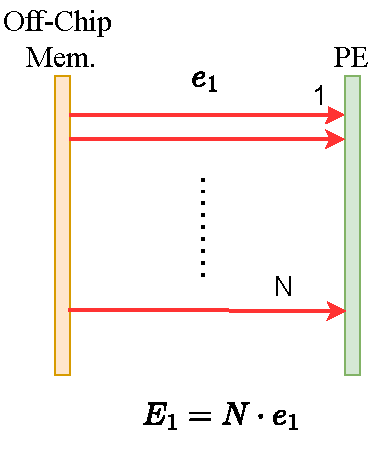
\includegraphics[width=0.25\textwidth]{memAccessSingleLevel}
		\label{fig:memsAccessSingle}}
	\hfil	
	\subfloat[]{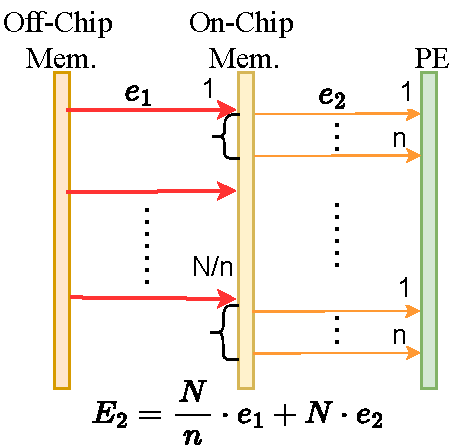
\includegraphics[width=0.3\textwidth]{memAccess2Level.pdf}
		\label{fig:memsAccessDouble}}
	\hfil	
	\caption{Memory accesses and energy estimates for accessing data (a) always from the off-chip memory. (b) from two-level of memory hierarchy while reusing the data from on-chip memory.}
	\label{fig:memsAccess}
\end{figure}

The NN accelerator reads the input data (or input activations), filter weights, and partial sums from the off-chip memory and stores them temporarily in the on-chip memory. The PE array reads the data from the on-chip memory to perform the computations and then stores them back to the on-chip memory. The partial sums or the outputs of the computations are then finally stored in the off-chip memory. The data flow is shown in \figref{fig:nnDataFlow}. Due to the significant difference between the energy consumption of accessing the data from the off-chip memory and the on-chip memory, NN accelerators aim to minimize the off-chip memory accesses by exploiting the memory hierarchy and data reuse from them.
\begin{figure}[!htb]
	\centering
	\captionsetup{font=sf}	
	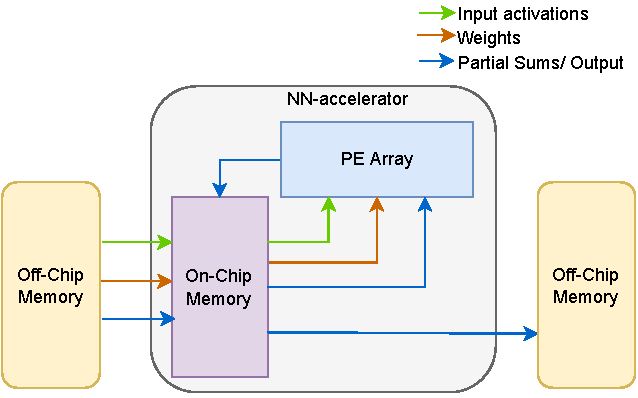
\includegraphics[width=0.5\textwidth]{nnDataFlow}
	\caption{Read/Write of inputs, weights, and partial/final outputs from different levels of memories.}
	\label{fig:nnDataFlow}
\end{figure}

The layer data is stored as multi-dimensional arrays in the off-chip memory, which is generally too large to fit in the local on-chip memory. In order to perform the computations, the large layer data is partitioned into small tiles. These tiles are repeatedly fetched from the off-chip memory to compute the final output sum. 

To observe the impact of tile dimensions on off-chip memory accesses for a given data reuse scheme, we measured the off-chip memory accesses for a popular CNN, VGG16, for different tile dimensions using the algorithm described in \secref{sec:Access3DData}. \figref{fig:impactOfTileDims} illustrates the impact of tile dimensions on off-chip memory accesses for VGG16. Meanwhile, \figref{fig:varyingTileDims} provides a closer look at the significant variations in off-chip memory accesses within a single layer when tiles of different dimensions are chosen. On the x-axis, we represent a subset of the valid tile search space for the layer, while the y-axis indicates the corresponding off-chip memory access for the selected tile dimensions.

This visualization demonstrates that the choice of tile dimensions plays a crucial role in determining off-chip memory accesses. A well-selected tile dimension can result in a substantial reduction, as much as 90\% in some cases, in off-chip memory accesses compared to a poorly chosen tile dimension. This observation is further supported by \figref{fig:maxNMinLayerAccess}, which showcases the computed values for different layers of VGG16. The depicted variations emphasize the importance of optimizing tile dimensions to enhance overall system efficiency and minimize off-chip memory access overhead.

\begin{figure}[!h]
	\centering
	\captionsetup{font=sf}
	\subfloat[]{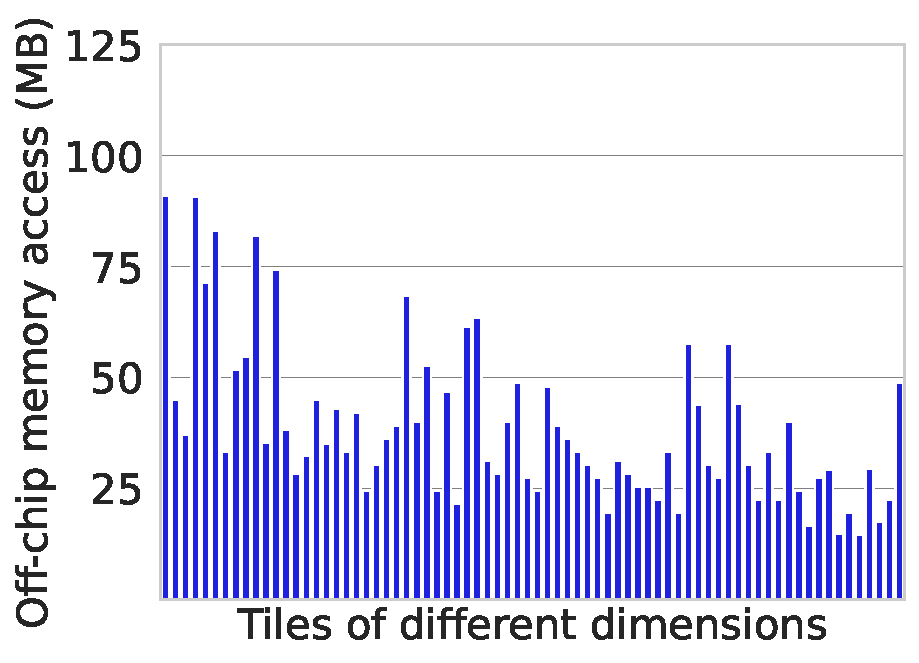
\includegraphics[width=0.4\textwidth]{varyingTileDims.pdf}
		\label{fig:varyingTileDims}}
	\hfil	
	\subfloat[]{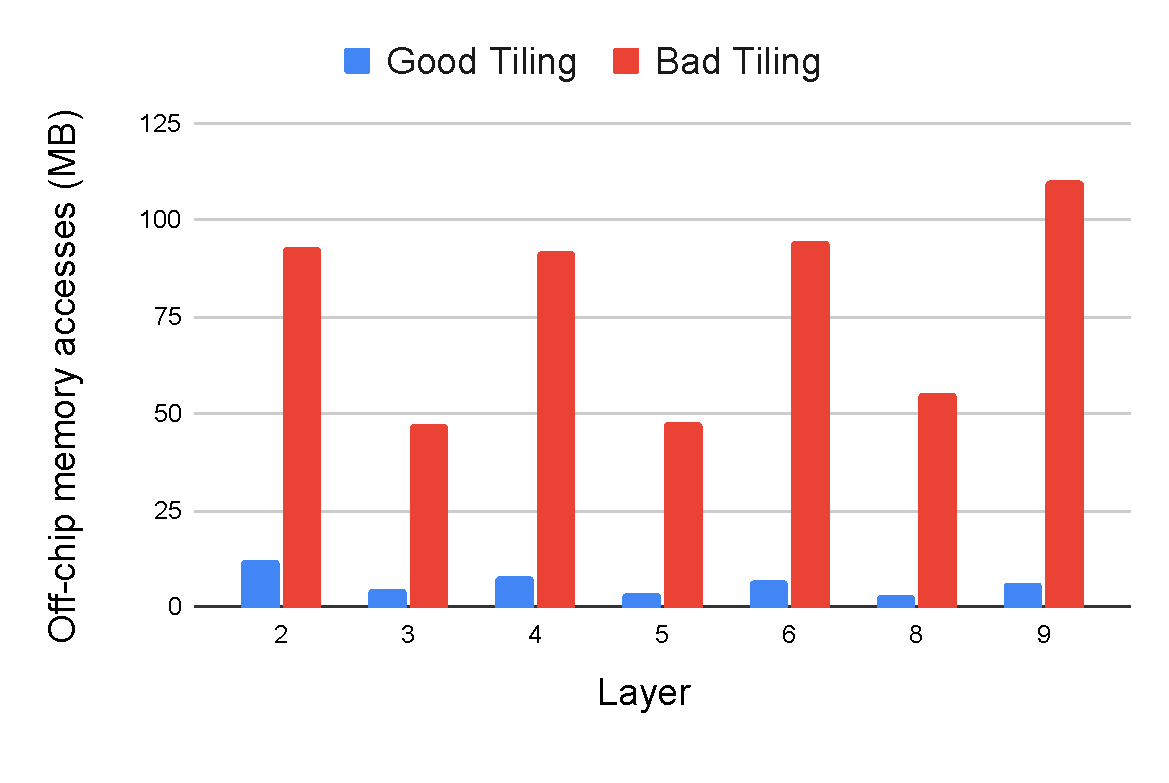
\includegraphics[width=0.4\textwidth]{impactOfTileDims.pdf}
		\label{fig:maxNMinLayerAccess}}
	\hfil	
	\caption{Impact of tile dimensions on off-chip memory accesses (a) off-chip memory access variations of a single convolution layer when accessing with tiles of different dimensions, x-axis represents a subset of valid tile space of the layer (b) Impact of good and bad tile dimensions on different convolution layers of VGG16.}
	\label{fig:impactOfTileDims}
\end{figure}

Determining the optimal tile dimensions and scheduling scheme requires comparing the off-chip memory accesses for different tile dimensions and scheduling schemes. Modern DNNs have a variety of layers (e.g., convolution, fully connected, recurrent, pooling), each exhibiting different types of data access patterns. Even the layers of the same type differ in shape and size. Due to varying layer shapes, sizes, and types, optimal partitioning, and scheduling vary among layers. Finding the optimal partitioning and scheduling scheme by performing the measurements on the hardware is time-consuming, and large search space makes it practically impossible.

To address this, we have developed an analytical framework that integrates models of NN layers to compute a layer's off-chip memory accesses, data access energy, and the number of compute cycles for mapping a layer on a NN accelerator (~\figref{fig:typicalDNNAccelerator}). \figref{fig:analyticalModel} shows the block diagram of the analytical framework. The framework is used as a design space exploration engine to find the optimal partitioning and scheduling scheme for a given layer type and layer shape to optimize NN accelerators' energy efficiency and throughput. 
\begin{figure}[!htb]
	\centering
    \captionsetup{font=sf}	
	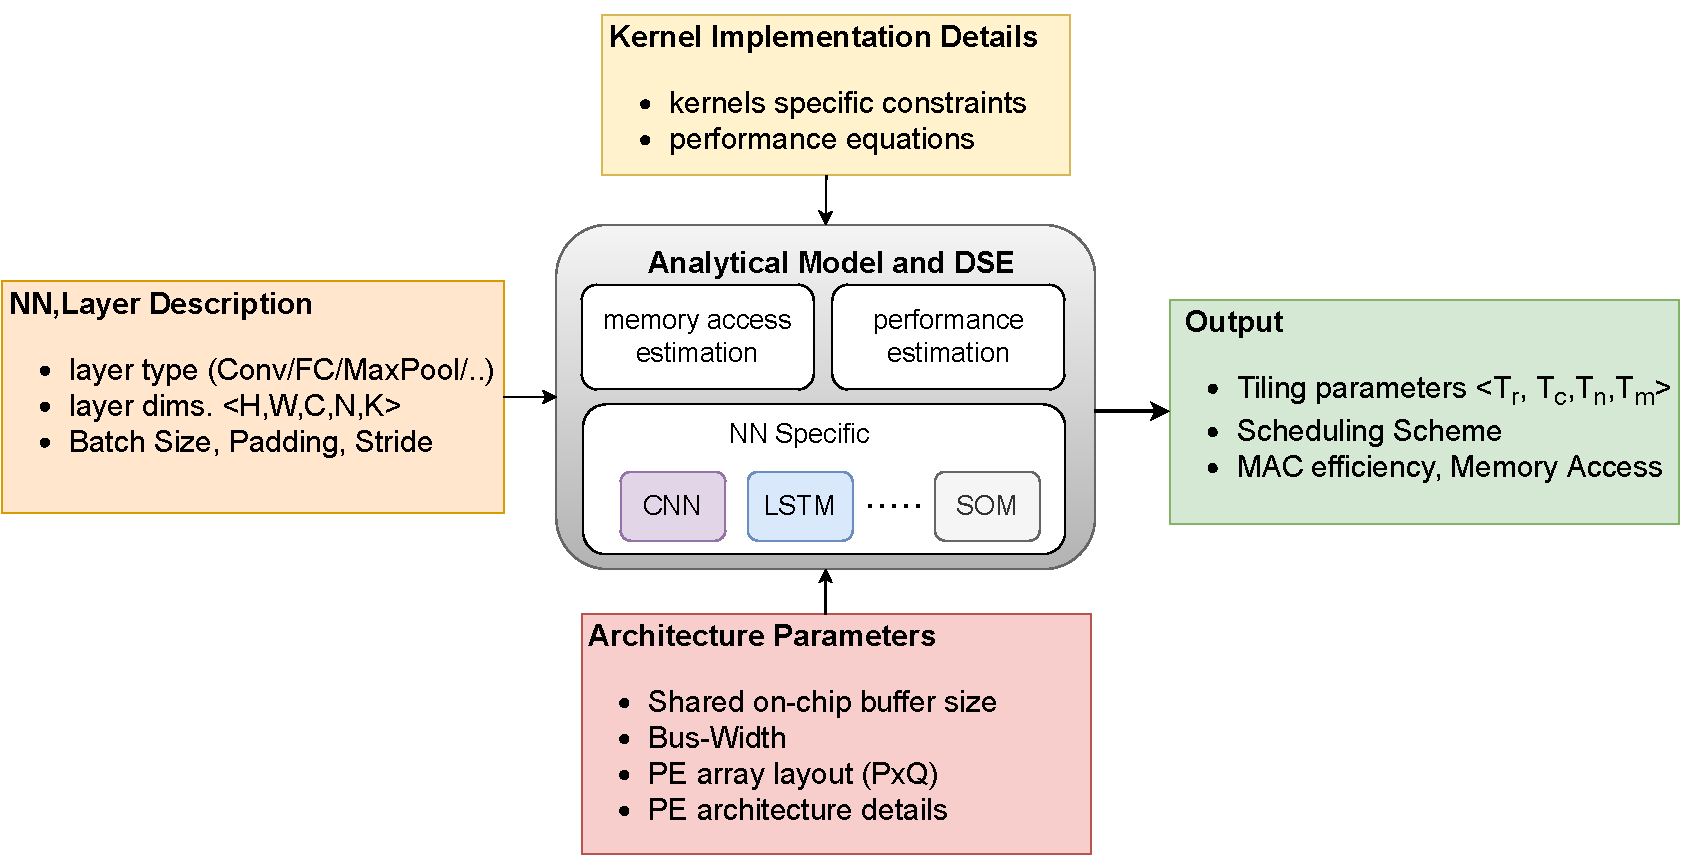
\includegraphics[width=0.9\textwidth]{analyticalModel}
	\caption{Analytical framework to estimate the performance, off-chip memory accesses and energy of DNNs.}
	\label{fig:analyticalModel}
\end{figure}

If a 3D data is partitioned into $N_{tiles}$ number of tiles, $r_t$ is the trips count and $\numBytesOffChip_{t}$ is the number of bytes accessed from off-chip memory for the $t^{th}$ tile, the off-chip memory access of partitioned 3D data can be computed as follows
\begin{align}\label{eq:BasicOffChip3DDataAccess_t}
	\numBytesOffChip_{3D}&{=}\sum_{t=1}^{N_{tiles}}(\numBytesOffChip_{t}{\times}r_t)
\end{align}
In DNN layers, $r_t$ depends on the layer shape, tile dimensions, and scheduling scheme, and it is the same for all the tiles of the 3D data ($r$). However, $B_t$ in \eqref{eq:BasicOffChip3DDataAccess_t} varies among the tiles depending on the architectural parameters and address alignment. ~\eqref{eq:BasicOffChip3DDataAccess_t} can be expressed as 
\begin{align}\label{eq:BasicOffChip3DDataAccess}
	\numBytesOffChip_{3D}&{=}r{\times}\sum_{t=1}^{N_{tiles}}\numBytesOffChip_{t}
\end{align}
The analytical framework computes the off-chip memory accesses of a given 3D data using~\eqref{eq:BasicOffChip3DDataAccess}, while considering the data resolution and architectural constraints. The framework considers the bus width and data alignment to precisely compute the off-chip memory accesses. It takes the address and shape of the data as input and iterates for all the tile dimensions. The analytical framework integrates models for different layer types and data reuse schemes to compute the memory accesses and data access energy. 

\section{Analytical study of architectural parameters}\label{sec:OffChipAccessModel}
\begin{figure}[!htb]
	\centering
	\captionsetup{font=sf}
	\begin{subfigure}[t]{0.45\textwidth}
		\centering
		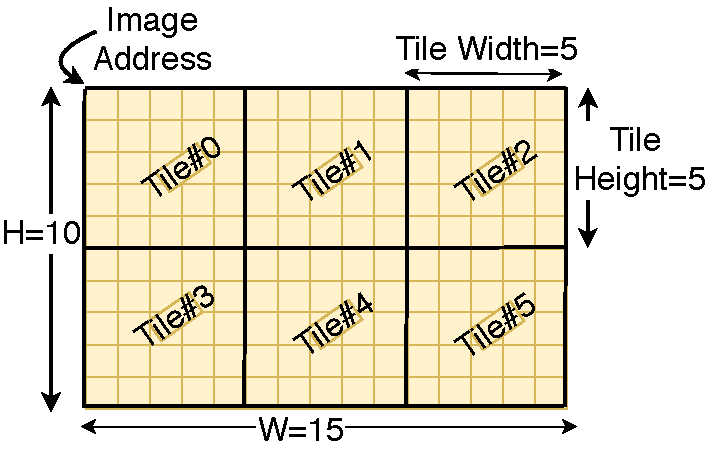
\includegraphics[width=\columnwidth]{A2DImage.pdf}
		\caption{A 2D image and its tiles}
		\label{fig:A2DImage}
	\end{subfigure}
	\hfil
	\begin{subfigure}[t]{0.4\textwidth}
		\centering
		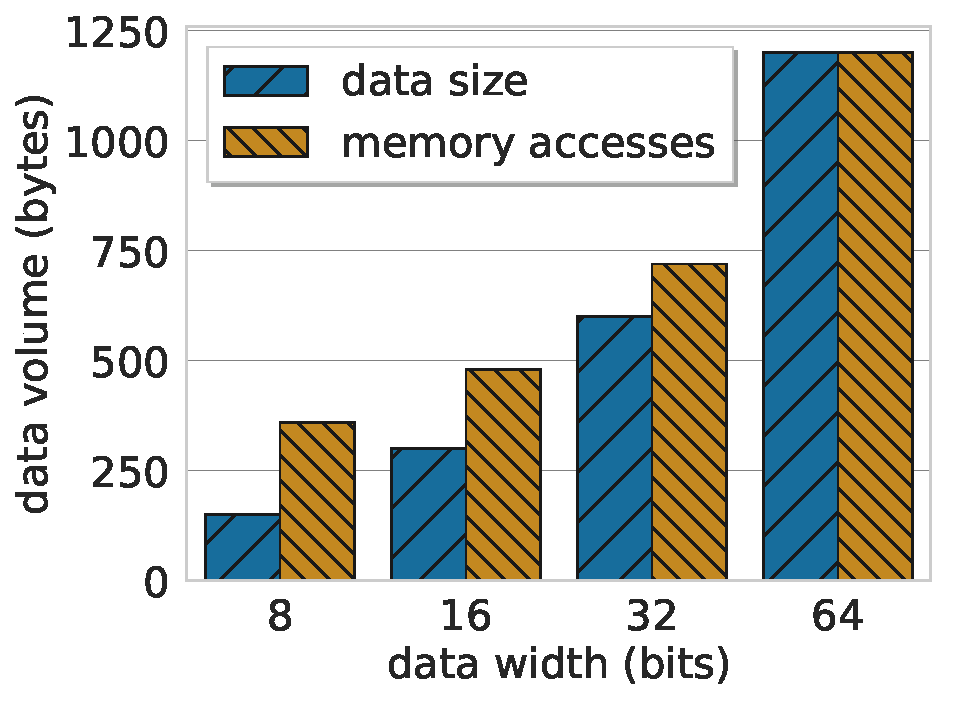
\includegraphics[width=\columnwidth]{MotivationExample.pdf}
		\caption{Data size vs. memory accesses}
		\label{fig:bitPerPixelEffect}
	\end{subfigure}		
	%	\begin{subfigure}[t]{0.3\textwidth}
		%		\centering
		%		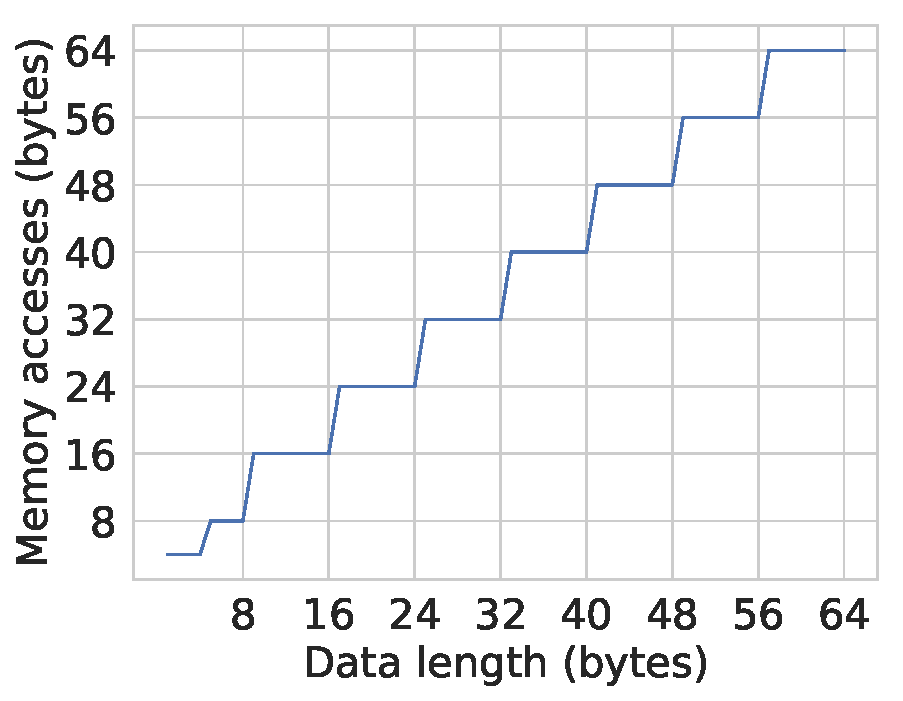
\includegraphics[width=\columnwidth]{Read1To64OnAXI.pdf}
		%		\caption{Memory accesses from aligned address}
		%		\label{fig:OffChipAccessVsLength}
		%	\end{subfigure}
	\caption{A 2D data and memory accesses on 64-bit data bus}
	\label{fig:2DPartitionedData}
	\vspace{-1.0em}	
\end{figure}

3D data of DNN layers and the tiles, into which the layer data is partitioned, is composed of stacked 2D frames. Off-chip memory access of the 3D data and its tiles can be computed by adding the off-chip memory accesses of 2D frames. \figref{fig:A2DImage} shows an example 2D frame of shape 10$\times$15, partitioned into tiles of dimensions 5$\times$5. Although all tiles have the same size, the off-chip memory accesses for different tiles are not the same. To observe the differences between the tile sizes and off-chip memory accesses of the tiles, we implemented a hardware design using Xilinx SDSoC framework, SDx v2018.3, to access the 2D data stored in DRAM. We measured the memory accesses using AXI Performance Monitor (APM) IP~\cite{APM}, integrated with our design. The target platform is ZedBoard, working at 100MHz frequency, and off-chip memory (DRAM) is accessed using 64 bits AXI bus. \tabref{tab:TileOffChipAccesses} shows each tile's sizes and off-chip memory accesses on 64 bits wide bus for 8 bits data width. The difference between the tile sizes and the memory accesses is due to the bus width and address alignments of different rows of the tile. 
\begin{table}[htb]
	\centering
	\caption{Off-Chip memory accesses of the tiles of size 5$\times$5 }
	\begin{tabular}{|c|c|c|c|c|c|c|c|}
		\hline
		\textbf{Tile\#}& 0  & 1  & 2  & 3  & 4  & 5  & \textbf{Total} \\ \hline
		\textbf{Size(bytes)}& 25 & 25 & 25 & 25 & 25 & 25 & 150   \\ \hline
		\textbf{Mem. Access(bytes)} & 72 & 56 & 56 & 48 & 72 & 56 & 360  \\
		\hline
	\end{tabular}
	\label{tab:TileOffChipAccesses}
\end{table}

\figref{fig:bitPerPixelEffect} shows the size and off-chip memory accesses of the 2D data shown in~\figref{fig:A2DImage}, for different data bit widths. The ratio of memory accesses to the data size for small data bit width is high. Modern NN accelerators use a wide memory bus to improve the memory bandwidth and a low number of bits to represent the data to reduce the storage requirements and memory accesses. Therefore it is crucial to consider the architectural parameters for low-resolution data.
\begin{figure}[!htb]
	\centering
	\captionsetup{font=sf}	
	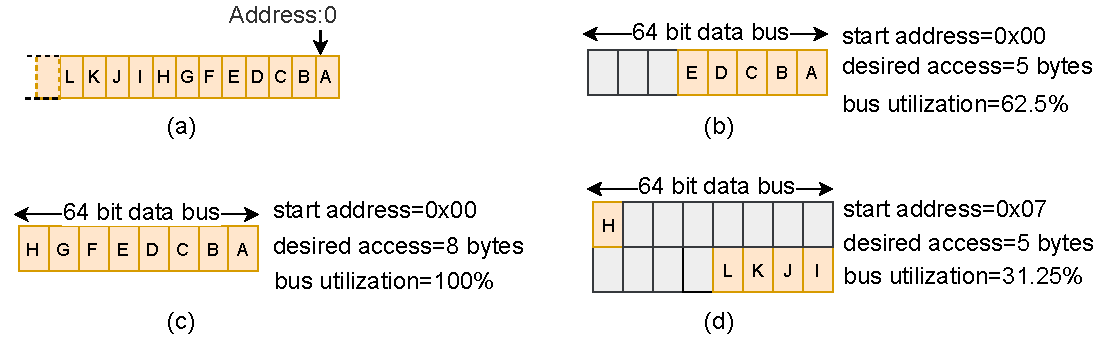
\includegraphics[width=0.9\textwidth]{BurstTranscationOnAXI}
	\caption{Off-chip memory accesses on 64-bit wide data bus}
	\label{fig:AXI_AccesseOn64BitDataBus}
\end{figure}

The DNN accelerators use a wide data bus to access off-chip memory to meet the high memory bandwidth requirement~\cite{Chen2016EyerissAS,chen2014diannao}. If the number of bytes accessed from an off-chip memory address is not a multiple of bus width or the address is not aligned to the word boundary, it results in unused bytes lanes of the data bus. \figref{fig:AXI_AccesseOn64BitDataBus} illustrates memory accesses on a 64-bit data bus. \figurename{~\ref{fig:AXI_AccesseOn64BitDataBus}a} shows a read transaction of 8 bytes from an aligned address and uses the full bus width. However, if only 5 bytes are read from an aligned address, as shown in \figurename{~\ref{fig:AXI_AccesseOn64BitDataBus}b}, 8 bytes are still accessed. If 5 bytes are read from an unaligned address, it results in 16 bytes of data access, as shown in \figurename{~\ref{fig:AXI_AccesseOn64BitDataBus}c}. The unused byte lanes do not carry any useful data, but contribute to overall energy consumption. The length of the data read should be chosen such that bus utilization is high and off-chip memory accesses and energy consumption are minimized.
\subsection{Aligned Access}
Number of bytes accessed from off-chip memory ($\numBytesOffChip_{align}$) from aligned addresses for different data length ($\dataLength$) is in multiples of bus width ($\busWidth$), e.g., reading 10 bytes results in 16 bytes of off-chip memory access.  $\numBytesOffChip_{align}$ for $\dataLength$ bytes and bus width $\busWidth$ can be expressed as
\begin{align}\label{eq:alignedAccess}
	\begin{aligned}[b]
		\numBytesOffChip_{align}(\dataLength,\busWidth) = \ceil[\big]{\frac{\dataLength}{\busWidth}}\times {\busWidth}
	\end{aligned}
\end{align}
\subsection{General Case}
To analyze the effect of bus width and address alignment, we express the number of bytes accessed from off-chip memory ($\numBytesOffChip$) for $\dataLength$ bytes of data as a function of $\dataLength$, its off-chip memory address ($\addressSym$), and the bus width ($\busWidth$).
The off-chip memory bus protocol supports burst based transactions where multiple data transfers of \emph{transfer size} happen from a starting address~\cite{AxiProtocolSpec}. Most transfers in a transaction are aligned to the \emph{transfer size}. However, the first transfer may be unaligned to the word boundary. 

The number of bytes accessed from off-chip memory for accessing $\dataLength$ bytes from address $\addressSym$ on $\busWidth$ bytes of bus width can be expressed as
\begin{equation}\label{eq:unalignedAccess}
	\begin{aligned}
		\numBytesOffChip(\addressSym,\dataLength,\busWidth)=(\ceil[\big]{\frac{\addressSym+\dataLength}{\busWidth}}-\floor[\big]{\frac{\addressSym}{\busWidth}})\cdot{\busWidth}
	\end{aligned}
\end{equation}
~\eqref{eq:alignedAccess} is a special case of~\eqref{eq:unalignedAccess} when memory access is from an aligned address.
\section{Off-Chip Memory Access of 3D Data}\label{sec:Access3DData}
\begin{figure}[!htb]
	\centering
	\captionsetup{font=sf}
	\begin{subfigure}[t]{0.5\columnwidth}
		\centering
		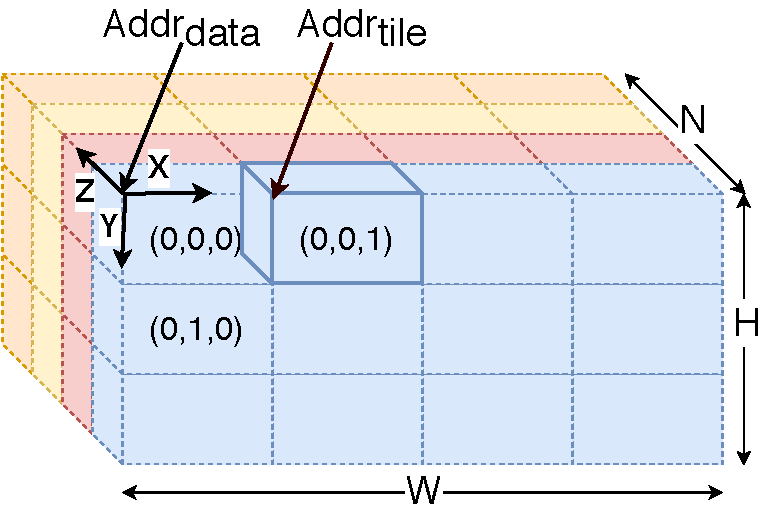
\includegraphics[width=0.6\columnwidth]{3DShapeAndZoomedTile1.pdf}
		\caption{A 3D data partitioned into tiles}
		\label{fig:3dTiledData}
	\end{subfigure}
	\begin{subfigure}[t]{0.4\columnwidth}
		\centering
		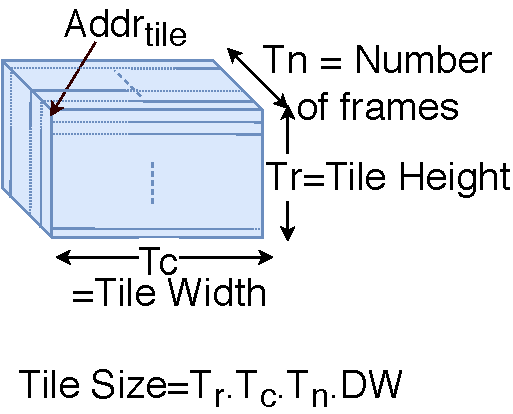
\includegraphics[width=0.6\columnwidth]{SingleTile.pdf}
		\caption{A 3D tile}
		\label{fig:3dTile}
	\end{subfigure}
	\caption{Off-Chip Accesses and a 3D partitioned data and tiles}
	\label{fig:3DPartitionedData}
\end{figure}
Consider a 3D data of shape $\langle W,H,N\rangle$, partitioned into tiles of dimension $\langle T_c,T_r,T_n\rangle$ as shown in~\figref{fig:3dTiledData} and~\figref{fig:3dTile}. Each tile is identified by index $(x,y,z)$ where $x, y, z \in \mathbb{Z}$ and 
\begin{align}\label{eq:TileIndexing}
	\begin{aligned}
		0\leq &x<\ceil[\big]{\frac{W}{T_c-\numOverlap}}, \\
		0\leq &y<\ceil[\big]{\frac{H}{T_r-\numOverlap}}, \\
		0\leq &z<\ceil[\big]{\frac{N}{T_n}}
	\end{aligned}
\end{align}
%$\numOverlap$ is the number of elements or rows overlapping between adjacent tiles. For CNNs, $\numOverlap$ is computed as $\numOverlap=(K-S)$, where $K$ is the filter dimensions and $S$ is the filter stride. Inter-tile overlap reuse, arising from the overlap between adjacent tiles, introduces dependencies in the order of accessing $ifm$ tiles. In our implementation, each tile is fetched separately, and we have not accounted for previously fetched data. This simplification is deliberate to avoid implementation complexity, with the assumption that any negligible impact on overall memory access can be safely disregarded.
$\numOverlap$ represents the number of elements or rows that overlap between adjacent tiles. In the context of Convolutional Neural Networks (CNNs) when accessing input feature maps ($ifm$) with a stride ($S$) less than the filter size ($K$), there occurs an overlap between adjacent tiles. The computation of $\numOverlap$ is given by $\numOverlap=(K-S)$, where $K$ denotes the filter dimensions and $S$ is the filter stride. This overlap introduces a reuse opportunity known as Inter-tile overlap reuse. In our implementation, each tile is fetched separately, and we have not accounted for previously fetched data. This simplification is deliberate to avoid implementation complexity, with the assumption that any negligible impact on overall memory access can be safely disregarded.

\algref{Algorithm1} computes the number of bytes accessed from off-chip memory for the 3D data. Each data element is represented by $DW$ bytes. The algorithm takes the address of the data ($Addr_{data}$), tile dimensions, data shape, and $\numOverlap$ as input and iterates lines~\ref{alg:ForAllTilesLoopk}--\ref{alg:loopkEnd} for all the tiles. It computes indices of the first element of the tile in the 3D array of the data using the tile index $(x,y,z)$ and $\numOverlap$ in lines~\ref{alg:idxc}--\ref{alg:idxn}. Using the indices of the first element, it computes the address of the tile in line~\ref{alg:tileAddr} and the dimensions of the tile in line~\ref{alg:tileDim}. The algorithm computes the total number of bytes accessed from off-chip memory by accumulating the number of bytes accessed for each tile in line~\ref{alg:tileAcc}. 

The address of the tile in line~\ref{alg:tileAddr} is computed by the function GetTileAddr using ~\eqref{eq:TileAddress}
\begin{align}\label{eq:TileAddress}
	\begin{split}
		%&Addr_{tile}=Addr_{data} + z\cdot T_{n}\cdot H \cdot W + y\cdot T_{r}\cdot W + x\cdot T_{c} \\
		GetTileAddr(Addr_{data},c,r,n,\langle W,H,N\rangle){=}Addr_{data} + c + r\cdot W + n\cdot W\cdot H
	\end{split}
\end{align}
If the data dimensions are not multiples of corresponding tile dimensions, the tiles at the border of the data (e.g., the right-most or bottom-most tiles) will have smaller dimensions. The function GetTileDim computes the dimensions of the tiles.

The function GetTileAcc in Lines~\ref{alg:FuncTileAccess}--\ref{alg:FuncTileAccessEnd} computes the addresses and number of bytes ($contSz$) for each off-chip memory transaction. $contSz$ is the number of contiguous bytes to access in a transaction. Let $T_n$ be the number of frames in the tile. If the tile width ($T_c$) is the same as the data width ($W$) (line~\ref{alg:TileAccessIf2}), then all the data elements of $T_r$ rows of a frame are contiguous, and the complete tile can be accessed using $T_n$ number of addresses. If the condition in line~\ref{alg:TileAccessIf1} is true, then all elements of the tile are contiguous and can be accessed using a single transaction of $T_c\cdot T_r\cdot T_n\cdot DW$ bytes (line~\ref{alg:TileAccessSingleTxn}). In all other cases, the tile is accessed using row addresses computed in line~\ref{alg:TileRowAddr}. The function computes the number of bytes accessed from off-chip memory for a tile ($Acc_{tile}$) in lines~\ref{alg:TileAccessIf1End},~\ref{alg:TileAccess2}, and~\ref{alg:TileAccessFor2End} using~\eqref{eq:unalignedAccess}. 
\begin{algorithm}[H]
	\caption{BW Aware off-chip memory access}
	 \label{Algorithm1}
	 \begin{algorithmic}[1]
	 	\Procedure{BWA}{$Addr_{data},\langle T_c,T_r,T_n\rangle,\langle W,H,N\rangle,\numOverlap$} \label{alg:BWA}
	 	\State $Acc_{data}\gets 0$
	 	\State $Addr_{tile}\gets Addr_{data}$
        \For{$x,y,z\leftarrow (0,0,0)$ ~\textbf{to} $(\ceil[\big]{\frac{W}{T_c-\numOverlap}}{-}1,\ceil[\big]{\frac{H}{T_r-\numOverlap}}{-}1,\ceil[\big]{\frac{N}{T_n}}{-}1)${\label{alg:ForAllTilesLoopk}}}
        \State $c\gets x\cdot (T_c-\numOverlap)$\label{alg:idxc}
        \State $r\gets y\cdot (T_r-\numOverlap)$\label{alg:idxr}
        \State $n\gets z\cdot T_n$\label{alg:idxn}
        \State $Addr_{tile}\gets \Call{GetTileAddr}{Addr_{data},c,r,n,\langle W,H,N\rangle}$\label{alg:tileAddr}
        \State $\langle T_c^1,T_r^1,T_n^1\rangle\gets$ \Call{GetTileDim}{$c,r,n,\langle T_c,T_r,T_n\rangle,\langle W,H,N\rangle$}\label{alg:tileDim}
        \State $Acc_{data}\gets Acc_{data}+$ \Call{GetTileAcc}{$Addr_{tile},\langle T_c^1,T_r^1,T_n^1\rangle,\langle W,H,N\rangle$}\label{alg:tileAcc}
	 	\label{alg:UpDiag_ReuseR2}   
	 	\EndFor \label{alg:loopkEnd}
	 	\State \textbf{return} $Acc_{data}$
	 	\EndProcedure
	 	
	 	\Procedure{GetTileAcc}{Addr$_{tile}$,$\langle T_c,T_r,T_n\rangle$,$\langle W,H,N\rangle$} \label{alg:FuncTileAccess}
	    \State $Acc_{tile}\gets 0$
	    \If{$T_c = W$ {\bf and} $T_r=H${\label{alg:TileAccessIf1}}}
	    	\State$contSz\gets T_c\cdot T_r\cdot T_n\cdot DW$\label{alg:TileAccessSingleTxn}
	    	\State$Acc_{tile}{\gets}$$\numBytesOffChip({Addr_{tile},contSz,BW})$\label{alg:TileAccessIf1End}
	    \Else
	    	    \For{$f\leftarrow 1$ ~\textbf{to} $T_n${\label{alg:TileAccessFor1}}}
	    	       \State Addr$_{f}{\gets} Addr_{tile}{+}(f{-}1){\cdot}H{\cdot}W$\label{alg:TileAccessFrameAddr}
	    	       \If{$T_c = W${\label{alg:TileAccessIf2}}}
   					    \State $contSz{\gets}T_c\cdot T_r\cdot DW$
                        \State $Acc_{tile}{\gets}Acc_{tile}+$$\numBytesOffChip({Addr_f,contSz,BW})$\label{alg:TileAccess2}
	    	       \Else
	    	           \State $contSz{\gets}T_c{\cdot}DW$
	    	           \For{$r\leftarrow 1$ ~\textbf{to} $T_r${\label{alg:TileAccessFor2}}}
                            \State $Addr_{(f,r)}{\gets}Addr_{f}+(r-1)\cdot W$\label{alg:TileRowAddr}
                            \State $Acc_{tile}{\gets}Acc_{tile}+$$\numBytesOffChip({Addr_{(f,r)},contSz,BW})$\label{alg:TileAccessFor2End}
	    	           \EndFor
	    	       \EndIf
	            \EndFor	
	    
	    \EndIf
	    \label{alg:FuncTileAccessEnd}	 	
	 	\State \textbf{return} $Acc_{tile}$
	 	\EndProcedure	
	
	
	 	\Procedure{GetTileDim}{$c,r,n$,$\langle T_c, T_r,T_n\rangle$,$\langle W,H,N\rangle$} \label{alg:FuncTileDimEnd}
	 	\State $T^1_c\gets min(T_c,W-c)$
	 	\State $T^1_r\gets min(T_r,H-r)$
	 	\State $T^1_n\gets min(T_n,N-n)$
	 	\State \textbf{return} ${\langle T^1_c,T^1_r,T^1_n\rangle}$
	 	\EndProcedure

	\end{algorithmic}
\end{algorithm}

DNN accelerators access layer data (ifm, ofm, and weights) partitioned into tiles. The tile dimensions should be chosen carefully to minimize the transfer of extra bytes to reduce off-chip memory access. We have proposed a bus width aware approach (BWA) that factors in the architectural parameters to precisely compute the off-chip memory access of 3D tiles and the layer data.

\section{Implementation and Results}
We have implemented a tool that calculates off-chip memory access for 3D data using the BWA algorithm (~\algref{Algorithm1}). This tool considers tile dimensions, layer shape, and the count of overlapping elements as inputs and is adaptable for different bus widths and data bit widths. Executed on a desktop machine, the tool quickly analyzes off-chip memory accesses for various tile dimensions. It seamlessly integrates with our analytical framework, estimating different NN layers' off-chip memory accesses, latencies, and data movement energies.

Validation of the off-chip memory access calculations of the tool was conducted by accessing the same shape of 3D data and using the same tile dimensions on a Xilinx FPGA. FPGA implementation was done using the Xilinx SDSoC framework, SDx v2018.3. The FPGA implementation utilized SDx pragmas for zero\_copy data movement and integrated the AXI Performance Monitor (APM) IP~\cite{APM} for real-time performance metrics, including bus latency and memory traffic. Executed on the ZedBoard platform at 100MHz, the off-chip memory (DRAM) was accessed using a 64-bit AXI bus. The FPGA implementation, taking 3D shape and tile dimensions as inputs, accesses 3D data from DRAM using loop tiling. Validation was performed by comparing the tool's calculated off-chip memory bytes with the APM-logged values for various 3D data shapes and tile dimensions.
\subsection{Results}
\figref{fig:measVsEst} illustrates the comparison between off-chip memory accesses computed by the analytical framework and measurements obtained on a Xilinx FPGA. For various layers of different shapes and sizes in the popular CNN, VGG16, reveal that the variation between off-chip memory accesses calculated by the analytical framework and the measured values on FPGA is consistently less than 4\%.  

Within the Convolution layers, three types of data are involved: filter weights ($wts$), input feature maps ($ifm$), and output feature maps ($ofm$). Our framework proves instrumental in not only accurately computing the off-chip memory accesses but also in analyzing the layer-wise distribution and breakdown of memory accesses for different types of data, filter weights ($wts$), input feature maps ($ifm$), and output feature maps ($ofm$), as depicted in \figref{fig:ifmOfmWtsDistribution}. The proposed framework is a valuable tool for quickly analyzing the memory accesses and data access energy for different tile dimensions and data reuse schemes to search for the optimal solution. 
\begin{figure}[!htb]
	\centering
	\captionsetup{font=sf}
	\subfloat[]{\includegraphics[width=0.4\textwidth]{VGG16_MeasVsEstMemAccess.pdf}
		\label{fig:measVsEst}}
	\hfil
	\subfloat[]{\includegraphics[width=0.4\textwidth]{VGG16_ifm_ofm_wts_splitMemAccess.pdf}
		\label{fig:ifmOfmWtsDistribution}}
	\hfil   
	\caption{Off-chip memory accesss of VGG16 layers (a) Comparison between the off-chip memory accesses estimated by the analytical framework and measured on FPGA. (b) Breakdown of off-chip memory access by data type estimated by the analytical framework.}
	\label{fig:nnLayerData}
\end{figure}
\section{Summary}
The chapter investigates the critical role of off-chip memory access in neural network (NN) accelerators, highlighting its impact on energy efficiency. The chapter addresses challenges arising from limited off-chip memory bandwidth and the energy-intensive nature of these accesses in NN accelerators. It introduces a sophisticated analytical framework that combines NN layer models to estimate performance metrics, off-chip memory accesses, and energy consumption. The proposed Bus Width Aware algorithm offers a precise method for computing off-chip memory accesses in 3D data, considering tile dimensions, layer shapes, and bus widths. The analytical tool's accuracy is validated through FPGA measurements, demonstrating less than 4\% variation. Overall, the chapter emphasizes the significance of optimizing memory access efficiency for NN accelerators and contributes a robust framework for achieving this goal.
\graphicspath{{./Ch3-CNN/images/}}

\chapter{Optimizing the Performance of CNN Accelerators} \label{chap:CNN}
CNNs are the state of the art machine learning algorithms. CNNs can achieve human-like accuracy in computer vision-related tasks. In order to achieve high accuracy, modern CNNs use a deep hierarchy of layers and perform compute-intensive and memory-intensive operations. CNN accelerators use many processing elements to exploit parallelism to speed up the computations. However, limited off-chip memory bandwidth limits their performance. In addition, considerable data transfer volume from the off-chip memory also results in high energy consumption.

CNNs have a sequence of mainly three types of layers: convolution layer (CL), pooling layer, and fully connected layer (FCL). There are several CLs, and a pooling layer usually follows each CL. The last few layers of the CNNs are FCLs. VGG16 has thirteen CLs, and the last three layers are FC. Similarly, AlexNet has five CLs, followed by 3 FCLs. Pooling layer computations involve sliding a two-dimensional filter window over a single channel of \textit{ifm} and selecting one activation from the window using an operation like maximum or average. There are no parameters in pooling layers. The pooling layer helps reduce the activation sizes and, thus, the number of parameters in subsequent layers. CL and FC layers are compute-intensive, requiring millions of parameters. 

\figref{fig:CLOps} and~\figref{fig:FCLOps} illustrate the computations of a CL and an FCL, respectively. Each CL and FCL layer takes 3D input frames (\textit{ifm}) and applies filter weights (\textit{wts}) to compute output frames (\textit{ofm}). 3D $ifm$, $wts$ and $ofm$ are composed of $2D$ matrices stacked together in depth dimension. The number of 2D matrices is referred to as channels or depth of the data type. The number of channels ($N_i$) in each filter and $ifm$ are the same.

The convolution is performed by element-wise product between $K{\times}K$ filter elements with a 2D window of $ifm$ of size $K{\times}K$, for all the $N_i$ channels and then adding resulting $K{\times}K{\times}N_i$ elements to compute one element of the $ofm$ channel. Other elements of the $ofm$ channel are computed by sliding the 2D filter over the spatial dimension of the $ifm$ ($H_i{\times}W_i$). Filter slides by S elements from left to right and then top to bottom. $K$ and $S$ are referred to as the filter size and stride of the filter, respectively. We assumed square filters of dimension $K{\times}K$, $K$ is an odd integer, filter stride in horizontal and vertical directions are identical, and $S{\le}K$, which are typically the case. 

\begin{figure}[!htb]
	\centering
	\captionsetup{font=sf}	
	\subfloat[Convolution Layer]{\includegraphics[width=0.49\textwidth]{CLOps.pdf}
		\label{fig:CLOps}}
	\hfil	
	\subfloat[Fully Connected Layer]{\includegraphics[width=0.42\textwidth]{FCLOps.pdf}
		\label{fig:FCLOps}}
	\hfil	
	\caption{Convolution and fully connected layers}
	\label{fig:CNNAcceleratorAndCLOps}
\end{figure}

$ofm$ dimensions of CL and FC layers can be computed using the $ifm$ dimensions, filter size ($K$), and stride ($S$). \figref{fig:CLInOutDimRel} illustrates the relation of ofm dimension with ifm and filter dimensions for stride $S{=}1$. The filter can be placed at $W_i{-}(K{-}1)$ horizontal locations and $H_i{-}(K{-}1)$ locations in the vertical dimensions of the $ifm$. If $S{=}1$, the $ofm$ spatial dimensions are $K{-}1$ elements less than the $ifm$ dimensions. Several CNN architectures add padding elements to the border of the $ifm$ spatial dimensions. If the padding on the left, right, top, and bottom are $P_l$, $P_r$, $P_t$, and $P_b$, respectively, the $ofm$ dimensions for $S{=}1$ can be computed as follows,
\begin{align}\label{eq:ifmOfmStrideOne}
	\begin{split}
W_o&=W_i+P_l+P_r-(K-1)\\
H_o&=H_i+P_t+P_b-(K-1)
\end{split}
\end{align}
\begin{figure}[!htb]
	\centering
	\captionsetup{font=sf}	
	{\includegraphics[width=0.8\textwidth]{convInAndOutDims.pdf}
		\label{fig:CLInOutRelHz}}
	\caption{Input and Output dimensions of CL layer for filter stride=1  }
	\label{fig:CLInOutDimRel}
\end{figure}
If the stride is not 1, the number of elements in the $ofm$ spatial dimensions reduces by a factor of $S$. If the filter stride is $S$, $ofm$ spatial dimensions can be expressed as follows, which is the generalization of the equation~\eqref{eq:ifmOfmStrideOne}
\begin{align}\label{eq:ifmOfmStrideS}
	\begin{split}
		W_o&=\ceil[\big]{\frac{W_i+P_l+P_r-(K-1)}{S}}\\
		H_o&=\ceil[\big]{\frac{H_i+P_t+P_b-(K-1)}{S}}
	\end{split}
\end{align}
If the padding at the top, bottom, left and right are the same as $P$, ~\eqref{eq:ifmOfmStrideS} can be simplified as follows,
\begin{align}\label{eq:ifmOfmStrideS_P}
	\begin{split}
		W_o&={\frac{W_i+2\cdot P-K}{S}}{+}1\\
		H_o&={\frac{H_i+2\cdot P-K}{S}{+}1}
	\end{split}
\end{align}

CNN accelerators have limited on-chip memory size. Layer activations and parameter sizes are too large to fit into the on-chip memory. CNN accelerators apply loop tiling to partition the layer data into small tiles that fit into on-chip memory. Loop tiling is a compiler  technique~\cite{aho2006compilers} that partitions the loop iteration space and large arrays into smaller tiles to increase the data locality and ensure data fits into smaller memories. \figref{fig:partitioningDataUsingTiling} shows a layer's data stored in off-chip memory and its tiles in the accelerator's on-chip buffer.
\begin{figure}[!htb]
	\centering
	\captionsetup{font=sf}	
	\includegraphics[width=0.5\textwidth]{AboutTheCNNTiles.pdf}
	\caption{CNN layer tiles in off-chip and on-chip memory}
	\label{fig:partitioningDataUsingTiling}
\end{figure}

Listing~\ref{code:CNNTiledCode} shows the Pseudo code of the tiled version of a convolution layer. The computations involve nested loops. The outer five loops labeled as $L_D,L_H,L_W,L_M,L_N$ select the tiles of the data, and inner loops perform computations on the selected tiles. The order of the outer loops decides the sequence in which different tiles are processed. Each of the $5!$ permutations of the outer loop results in a valid schedule. 
%\begin{minipage}{0.9\columnwidth}
\begin{lstlisting}[float,language=C,label=code:CNNTiledCode,caption=Pseudo code of a tiled convolution layer,captionpos=b,belowskip=-1 \baselineskip,breakautoindent=true, breakindent=108pt, breaklines]
	L_D:for(d=0;d<D;d++) {
		L_H: for(row=0;row<H;row+=Tr) {
			L_W:  for(col=0;col<W;col+=Tc) {
				L_N:  for(ti=0;ti<N;ti+=Tn) {
					L_M:  for(to=0;to<M;to+=Tm) {
						//load wts tile
						//load ifm tile
						//load ofm tile
						for(trr=row;trr<min(row+Tr,H);trr++) {
							for(tcc=col;tcc<min(col+Tc,W);tcc++) {
								for(too=to;too<min(to+Tm,M);too++) {
									for(tii=ti;tii<min(ti+Tn,N);tii++) {
										for(i=0;i<K;i++) {
											for(j=0;j<K;j++) {
												ofm[d][to][row][col] += weights[to][ti][i][j] * 
												                  ifm[d][ti][S*row+i][S*col+j];
						} } } } } }
						//store ofm tile}
	} } } }}
\end{lstlisting}

There are $4!$ permutations in which loop $L_M$ appears as the innermost loop. In these permutations, all iterations of the innermost loop $L_M$ use the same \textit{ifm} data. In all such loop orderings, the load statement of \textit{ifm} tile can be moved before the innermost loop $L_M$ and reused in all its iterations \cite{zhang2015optimizing}. The movement of ifm tile loading reduces the number of off-chip accesses of ifm tile by a factor of $\frac{M}{T_m}$. This ordering scheme exploits ifm data reuse and is referred to as Input reuse-oriented scheme (IRO). Similarly, the set of $4!$ permutations in which loop $L_N$ is an innermost loop exploits the data reuse of \textit{ofm} and is referred to as output reuse oriented (ORO). The remaining $3\times 4!$ permutations in which loops $L_D, L_R, L_C$ appear as the inner loops exploit the weight data reuse and are referred to as the Weight Reuse Oriented scheme(WRO). The amount of data reused in different schemes varies with layer shape.
%The order of loops determines the scheduling of the tiles. The scheduling scheme, which minimizes the trips of the \textit{ifm} tiles between the accelerator and off-chip memory, is referred to as the input-reuse-oriented scheme (IRO). Similarly, the other two schemes, which minimize the trips of \textit{ofm} and \textit{wts}, are referred to as output-reuse-oriented (ORO) and weight-reuse-oriented (WRO) schemes, respectively. 

CNN's layers have varying shapes. \figref{fig:ParamsNactProp} shows the parameters and activation proportions in convolution (CL) and fully connected layers (FC) of VGG16 and AlexNet. The first few layers have a large volume of activations (\textit{ifm} and \textit{ofm}), and the last few CLs and FCLs have a large volume of parameters(\textit{wts} and \textit{biases}). Scheduling schemes that optimize the off-chip memory access of activations will work well in the first few layers but may not work well for deeper layers with a large volume of \textit{wts}. The scheduling scheme optimal for one layer may be suboptimal for other layers. Therefore, each layer needs to be analyzed here.
\begin{figure}[!htb]
	\centering
	\captionsetup{font=sf}	
	\subfloat[VGG16]{\includegraphics[width=0.49\textwidth]{VGG16ParamsNActivations}
		\label{fig:VGG16ParamsNActivations}}
	\hfil	
	\subfloat[AlexNet]{\includegraphics[width=0.49\textwidth]{AlexNetParamsNact.pdf}
		\label{fig:AlexNetParamsNact}}
	\hfil	
	\caption{Parameters and activations proportions in CL and FC layers of CNNs.}
	\label{fig:ParamsNactProp}
\end{figure}
\section{Related Work}
%Zhang et al.~\cite{zhang2015optimizing} used loop tiling to optimize the off-chip memory accesses. They expressed the off-chip memory access as a function of tile dimensions and layer shape and determined optimal tile dimensions by enumerating all the legal tile dimensions. They determined a global optimal tile dimension to reduce the hardware design complexity and used a common data reuse scheme for all the layers. Due to varying layer shapes, the optimal tile dimension and data-reuse scheme for different layers vary. To overcome this, Li et al.~\cite{Li2018SmartShuttleOO} proposed a layer-wise adaptive data partitioning and scheduling scheme. However, their approach ignored the architectural parameters and address alignment and assumed that all tiles of the same dimensions have the same off-chip memory accesses. With this assumption, the tile dimensions determined by their approaches are suboptimal.
Several studies (\cite{Li2018SmartShuttleOO, zhang2015optimizing, 7092377, MaYufei, 7302332, 7428073, 6657019}) have addressed the substantial impact of data transfer on the performance and energy efficiency of DNN accelerators. These works aimed to optimize off-chip memory accesses through loop ordering and tiling techniques.

Peeman et al.~\cite{7092377} presented an analytical method to optimize the convolution nested loops for inter-tile data reuse using loop transformations. The inter-tile reuse scheme they proposed creates dependencies between the tiles and reduces the inter-tile parallelism. Ma et al.~\cite{MaYufei} ignored tile overlap, utilizing a fixed loop ordering and loop tiling scheme. They stored the full depth of $ifm$ tiles to minimize partial sum access from off-chip memory, but this approach may not scale for layers with numerous feature maps.
 
Shi et al.~\cite{7302332} proposed intra-output feature map parallelism to leverage data locality, aiming to reduce off-chip DRAM accesses by reusing data from on-chip buffers. However, their design has limitations, including using separate buffers for input and output feature maps, reducing flexibility. Additionally, their analysis focused solely on height and width tile dimensions, employing a fixed loop ordering and tiling scheme that may not be optimal for various layer shapes in CNNs. 

Zhang et al.~\cite{zhang2015optimizing} expressed off-chip memory access as a function of tile dimensions and layer shape, determining optimal tile dimensions by enumerating legal options. They sought a global optimal tile dimension to simplify hardware design, utilizing a common data reuse scheme for all layers. However, the optimal tile dimensions and data-reuse schemes differ across layers due to varying layer shapes.

Motamedi et al.~\cite{7428073} considered the impact of adaptive tiling and demonstrated its superior performance compared to static solutions. However, their adaptive tiling was limited to feature maps' height and width dimensions.

The closest approach to ours is the layer-wise adaptive data partitioning and scheduling scheme by Li et al.~\cite{Li2018SmartShuttleOO}. Nevertheless, their method overlooked architectural parameters and address alignment, assuming identical off-chip memory accesses for tiles of the same dimensions. This assumption may lead to suboptimal tile dimensions in their approach.

Our approach considers an adaptive strategy for loop tiling and loop ordering for all the layers, analyzing the impact of architectural parameters on off-chip memory access. We use this information to determine optimal tile dimensions and data reuse scheme, aiming to reduce off-chip memory accesses for different layers of CNNs.

\section{Off-Chip Memory Accesses of CNN Layers}\label{MemAccess_CNN}
%\subsection{Off-chip memory access of CL}\label{sec:AccessCLData}
\begin{comment}
A CNN accelerator accesses 3D data of \textit{ifm, ofm}, and \textit{wts} of each layer partitioned into tiles. It accesses tiles of the layer from off-chip memory one or multiple times. Trip counts of the tiles depend on the layer shape, tile dimensions, and the data reuse scheme. If the batch size is $D$, layer shape is $\langle W_o,H_o,N_i,M_o\rangle$ and tiling parameters are $\langle T_{c_o},T_{r_o},T_{n_i},T_{m_o}\rangle$, trip counts of tiles in IRO, ORO, and WRO schemes can be expressed as the rows of the matrix $\mathbf{R}$ in ~\eqref{eq:TripCount}, where columns represent \textit{ifm, ofm}, and \textit{wts} trip counts.
\begin{align}\label{eq:TripCount}
	\mathbf{R}=
	\begin{bmatrix}
		\mathbf{r}_{iro} \\  \mathbf{r}_{oro} \\ \mathbf{r}_{wro} \\
	\end{bmatrix}=
	\begin{bmatrix}
		D&(2\ceil[\big]{\frac{N_i}{T_{n_i}}}-1)D&\ceil[\big]{\frac{H_o}{T_{r_o}}}\ceil[\big]{\frac{W_o}{T_{c_o}}}D\\[6pt]
		\ceil[\big]{\frac{M_o}{T_{m_o}}}D&D&\ceil[\big]{\frac{H_o}{T_{r_o}}}\ceil[\big]{\frac{W_o}{T_{c_o}}} D\\[6pt]
		\ceil[\big]{\frac{M_o}{T_{m_o}}}D&(2\ceil[\big]{\frac{N_i}{T_{n_i}}}-1)D&1\\
	\end{bmatrix}
\end{align}
\end{comment}
CNN accelerators access 3D data of \textit{ifm, ofm}, and \textit{wts} of each layer partitioned into tiles. It accesses tiles of the layer from off-chip memory one or multiple times. Trip counts of the tiles depend on the layer shape, tile dimensions, and the data reuse scheme. If the batch size is $D$, layer shape is $\langle W_o,H_o,N_i,M_o\rangle$, and tiling parameters are $\langle T_{c_o},T_{r_o},T_{n_i},T_{m_o}\rangle$, trip counts of tiles in IRO, ORO, and WRO schemes can be determined using layer shape and tiling parameters. 
\subsection{Trip Counts of Tiles}\label{sec:TripCount}
\figref{fig:convPartitionedLayer} shows a toy convolution layer data partitioned into tiles. The $ifm$ is partitioned into two tiles in spatial dimension and two in depth. There are two filters $wts_C$ and $wts_D$ in the layer, and each is partitioned into two tiles in depth. The convolution output is computed and stored as 4 $ofm$ tiles.
\begin{figure}[!htb]
	\centering
	\captionsetup{font=sf}	
	\includegraphics[width=0.7\textwidth]{Conv2by2.pdf}
	\caption{A Convolution layer data partitioned into tiles }
	\label{fig:convPartitionedLayer}
\end{figure}
\figref{fig:differentScheduling} shows three different valid schedules for the tiles of the convolution layer shown in \figref{fig:convPartitionedLayer}. 
\begin{figure}[!htb]
	\centering
	\captionsetup{font=sf}
	\subfloat[IRO Scheduling]{\includegraphics[width=0.25\textwidth]{IROScheduling.pdf}
	\label{fig:IROScheduling}}
    \hfil		
	\subfloat[ORO Scheduling]{\includegraphics[width=0.25\textwidth]{OROScheduling.pdf}
		\label{fig:OROScheduling}}
	\hfil	
	\subfloat[WRO Scheduling]{\includegraphics[width=0.25\textwidth]{WROScheduling.pdf}
		\label{fig:WROScheduling}}
	\hfil	
	\caption{Different Scheduling of tiles.}
	\label{fig:differentScheduling}
\end{figure}

There are several ways in which a  combination of $ifm$, $ofm$, and $wts$ tiles can be accessed from the off-chip memory to perform the computations by the accelerator, resulting in a valid schedule. These schedules differ in how tile combinations are fetched from the off-chip memory and the volume of off-chip memory accesses. \figref{fig:differentScheduling} shows three different schedules, which minimizes the off-chip memory accesses of one data type.

\figref{fig:IROScheduling} shows the Input Reuse Oriented (IRO) scheme schedule, which maximizes the input data reuse. In the IRO scheduling scheme, all the operations involving a given $ifm$ tile are scheduled consecutively to access each $ifm$ tile only once from the off-chip memory. There are $\ceil[\big]{\frac{H_o}{T_{r_o}}}\ceil[\big]{\frac{W_o}{T_{c_o}}}$ number of $ifm$ tiles in spatial dimension and $\ceil[\big]{\frac{N_i}{T_{n_i}}}$ number of $ifm$ tiles in depth dimension. Each $wts$ tile is accessed repeatedly from the off-chip memory to convolve with different spatial $ifm$ tiles, and each $ofm$ tile is accessed repeatedly to compute the final outputs using the $ifm$ tiles in the depth dimension. Unlike the $wts$ tile, which are only read from the off-chip memory, each $ofm$ tile needs to be written to and read from the off-chip memory, except the first time when it is only written. The trip count of $ifm$, $ofm$ and $wts$ tiles in IRO scheme can be computed as following,
\begin{align}\label{eq:IROTripCount}
	\begin{split}
	r_{ifm} &= D \\
	r_{ofm}&= (2\ceil[\big]{\frac{N_i}{T_{n_i}}}-1)D \\
	r_{wts} &= \ceil[\big]{\frac{H_o}{T_{r_o}}}\ceil[\big]{\frac{W_o}{T_{c_o}}}D
	\end{split}
\end{align}
\figurename~\ref{fig:OROScheduling} shows the Output Reuse Oriented (ORO) scheme, which maximizes the reuse of partial sums. In the ORO scheduling scheme, all the partial sums required for an $ofm$ tile are performed consecutively, and the final sum is written once to the off-chip memory. Computing a single $ofm$ tile requires convolving all the $ifm$ and $wts$ tiles in the input depth dimension. This results in repeatedly accessing the $ifm$ and $wts$ tiles from the off-chip memory. In this scheme, each $ifm$ tile is accessed $\ceil[\big]{\frac{M_o}{T_{m_o}}}$ times to convolve with all the filters and each $wts$ tile is accessed $\ceil[\big]{\frac{H_o}{T_{r_o}}}\ceil[\big]{\frac{W_o}{T_{c_o}}}$ times to perform the operations with all the $ifm$ tiles in spatial dimensions. The trip count of $ifm$, $ofm$, and $wts$ tiles for the ORO scheduling scheme can be computed as following,
\begin{align}\label{eq:OROTripCount}
	\begin{split}
		r_{ifm} &= \ceil[\big]{\frac{M_o}{T_{m_o}}}D \\
		r_{ofm}&= D \\
		r_{wts} &= \ceil[\big]{\frac{H_o}{T_{r_o}}}\ceil[\big]{\frac{W_o}{T_{c_o}}} D
	\end{split}
\end{align}
\figref{fig:WROScheduling} shows the Weight Reuse Oriented (WRO) scheme that maximizes the weights reuse. Each $wts$ tile is accessed once from the off-chip memory, and all the operations involving the $wts$ tile are performed consecutively. This requires repeatedly accessing the $ifm$ and $ofm$ tiles from the off-chip memory. Each $ifm$ tile  is accessed $\ceil[\big]{\frac{M_o}{T_{m_o}}}$ times, once for each $wts$ tile. There are $\ceil[\big]{\frac{N_i}{T_{n_i}}}$ tiles in the input depth. The partial sums resulting from each $ifm$ tile in the input depth need to be read from and written to off-chip memory, except for the first tile, which is only written to the off-chip memory. Total trip counts of the output partial sums tiles are $(2\ceil[\big]{\frac{N_i}{T_{n_i}}}-1)$. In this case, the trip count of $ifm$, $ofm$ and $wts$ tiles can be computed as following,
\begin{align}\label{eq:WROTripCount}
	\begin{split}
		r_{ifm} &= \ceil[\big]{\frac{M_o}{T_{m_o}}}D\\
		r_{ofm}&= (2\ceil[\big]{\frac{N_i}{T_{n_i}}}-1)D \\
		r_{wts} &= 1
	\end{split}
\end{align}
Trip counts of $ifm$, $ofm$, and $wts$ tiles in IRO, ORO, and WRO schemes can be expressed as the rows of the matrix $\mathbf{R}$ using~\eqref{eq:IROTripCount},~\eqref{eq:OROTripCount}, and~\eqref{eq:WROTripCount}, where columns represent \textit{ifm, ofm}, and \textit{wts} trip counts as shown in~\eqref{eq:TripCount} below.
\begin{align}\label{eq:TripCount}
	\mathbf{R}=
	\begin{bmatrix}
		\mathbf{r}_{iro} \\  \mathbf{r}_{oro} \\ \mathbf{r}_{wro} \\
	\end{bmatrix}=
	\begin{bmatrix}
		D&(2\ceil[\big]{\frac{N_i}{T_{n_i}}}-1)D&\ceil[\big]{\frac{H_o}{T_{r_o}}}\ceil[\big]{\frac{W_o}{T_{c_o}}}D\\[6pt]
		\ceil[\big]{\frac{M_o}{T_{m_o}}}D&D&\ceil[\big]{\frac{H_o}{T_{r_o}}}\ceil[\big]{\frac{W_o}{T_{c_o}}} D\\[6pt]
		\ceil[\big]{\frac{M_o}{T_{m_o}}}D&(2\ceil[\big]{\frac{N_i}{T_{n_i}}}-1)D&1\\
	\end{bmatrix}
\end{align}
\subsection{Off-chip memory access of CL}\label{sec:AccessCLData}
To compute the off-chip memory accesses for a CL layer, first, we compute the off-chip memory accesses for one trip of $ifm$, $ofm$ and $wts$ using~\algref{Algorithm1} of~\chapref{chap:analyticalFw} as below
\begin{align}\label{eq:MemAccessCL}
	\begin{split}
		\numBytesOffChip_{ifm}=&\emph{BWA}(\addressSym_{ifm},\langle T_{c_i}, T_{r_i},T_{n_i}\rangle,\langle W_i,H_i,N_i\rangle,\numOverlap)\\
		\numBytesOffChip_{ofm}=&\emph{BWA}(\addressSym_{ofm},\langle T_{c_o},T_{r_o},T_{m_o}\rangle,\langle W_o,H_o,M_o\rangle,0)\\
		\numBytesOffChip_{wts}=&M_o\cdot \emph{BWA}(\addressSym_{wts},\langle K,K,T_{n_i}\rangle,\langle K,K,N_i\rangle,0)
	\end{split}
\end{align} 
where $\numOverlap=(K-S)$ is the number of overlapping elements between adjacent $ifm$ tiles. $\numBytesOffChip_{ifm}$, $\numBytesOffChip_{ofm}$, and $\numBytesOffChip_{wts}$ are the number of bytes accessed from off-chip memory for one trip of \textit{ifm, ofm} and \textit{wts} respectively. $\langle W_{i},H_{i},N_{i}\rangle$ are the \textit{ifm} data shape and $\langle T_{c_i},T_{r_i},T_{n_i}\rangle$ are the \textit{ifm} tile dimensions. \textit{ofm} layer shape $\langle W_{o},H_{o},M_{o}\rangle$ is computed using~\eqref{eq:ifmOfmStrideS_P} and $ofm$ tile dimensions can be computed using~\eqref{eq:ifmOfmStrideS_P} as below,
\begin{align}\label{eq:ofmAndifmTileDims}
	\begin{split}
		T_{c_o}&=\frac{T_{c_{i}}-K}{S}+1 \\
		T_{r_o}&=\frac{T_{r_{i}}-K}{S}+1,
	\end{split}
\end{align}  
The total number of bytes accessed for j$^{th}$ reuse scheme ($\numBytesOffChip_j$) can be expressed as following sum
\begin{equation} \label{eq:TotalOffChipAccess}
	\numBytesOffChip_j=\mathbf{r_j}\cdot \begin{bmatrix}
		\numBytesOffChip_{ifm} &
		\numBytesOffChip_{ofm} &
		\numBytesOffChip_{wts}
	\end{bmatrix}^{T}
\end{equation}
where \textbf{r}$_j$ is the row vector of the matrix $\mathbf{R}$ (\eqref{eq:TripCount}) for the j$^{th}$ scheme. 
\subsection{Optimization problem}
Now, we present determining the optimal tile dimensions as a constraint optimization problem. Tiles of \textit{ifm, ofm} and \textit{wts} reside in on-chip memory. The volume of the tiles is given by equation~\eqref{eq:tilesVol} below,
\begin{align}\label{eq:tilesVol}
	\begin{bmatrix}
		V_i \\ V_o \\ V_w
	\end{bmatrix}=
	\begin{bmatrix}
		T_{c_i}\cdot T_{r_i}\cdot T_{n_i}\\
		T_{c_o}\cdot T_{r_o}\cdot T_{m_o}\\
		K^2\cdot T_{n_i}\cdot T_{m_o}\\
	\end{bmatrix}
\end{align}
where $V_i, V_o, \text{and }V_w$ are the sizes of \textit{ifm, ofm}, and \textit{wts} tiles, respectively. If the on-chip memory buffer size is $\BuffSize$ and each data element is represented by $\dataWidth$ bytes, then constraints on tile dimensions are
\begin{align}\label{eq:onChipConstraint}
	\begin{split}
		&(V_i + V_w + V_o)\cdot \dataWidth\leq \BuffSize \\
		&0<T_{c_o}\leq W_o,~\ 0<T_{r_o}\leq H_o\\
		&0<T_{n_i}\leq N_i,~\ 0<T_{m_o}\leq M_o
	\end{split}
\end{align}
Determining the tile dimensions which minimize the off-chip memory accesses, expressed by \eqref{eq:TotalOffChipAccess}, is a constraint optimization problem. The number of bytes accessed from off-chip memory using j$^{th}$ reuse scheme $\numBytesOffChip_j$ (~\eqref{eq:TotalOffChipAccess}) and the constraints (~\eqref{eq:onChipConstraint}) are non-linear functions of four variables $\langle T_{c_o},T_{r_o},T_{n_i},T_{m_o}\rangle$, and thus solving it is non-trivial.
\subsection{Off-chip memory access of FCL}\label{sec:AccessFCLData}
The computations of FCLs are a special case of CLs with additional constraints on layer shapes and parameters. The \textit{ifm} volume is same as a filter volume i.e., $H_i{=}W_i{=}K$, padding $P{=}0$, and stride $S{=}1$. In CNNs, typical values of K are 1, 3, 5, 7, and 11. Due to small values of $H_i$ and $W_i$, these dimensions are not partitioned ($T_{r_i}{=}T_{c_i}{=}K$). \textit{ofm} layer shape and tile dimensions computed using ~\eqref{eq:ofmAndifmTileDims} are $\langle 1,1,M_o\rangle$ and $\langle 1,1,T_{m_o}\rangle$.

For FCLs, the trip count of different data reuse schemes can be computed using~\eqref{eq:TripCount} and the number of bytes accessed from off-chip memory ($\numBytesOffChip^{FC}$) using~\eqref{eq:TotalOffChipAccess} by applying the layer shape constraints. The constraints on tile dimensions are given by~\eqref{eq:onChipConstraint}. $T_{n_i}$ and $T_{m_o}$ are the unknowns to be determined in~\eqref{eq:TotalOffChipAccess}. Determining the optimal tile dimensions for FCLs is a constraint optimization problem similar to CL.
\section{Implementation and Results}
\subsection{Implementation}
The optimal tile dimensions need to be determined once for a given NN and accelerator architecture, before the inference phase on edge devices. It can be determined by computing the number of bytes accessed from off-chip memory ($\numBytesOffChip$) at all the feasible points in the solution space. 
We have developed a tool that determines the optimal tile dimensions of each NN layer during the \emph{Preprocessing and Optimization} phase before the inference phase (~\figref{fig:workFlow} of~\chapref{chap:introduction}). The tool first prunes the large search space of tiles by applying the constraints (~\eqref{eq:onChipConstraint}). It then computes $\numBytesOffChip$ using \eqref{eq:TotalOffChipAccess} for each tile in the pruned search space and determines the optimal tile dimensions. The optimal tile dimension is determined for all the CL and FC layers of the NN. The tool also analyses the $\numBytesOffChip$ for different data reuse schemes to suggest the best scheme for each CL. It can be configured for different on-chip memory sizes, bus widths, and data bit widths. It took less than 10 minutes to determine the optimal solution for VGG16 on an Intel Core i7-6700 CPU (@3.40GHz$\times$8).
\subsection{Validation}\label{Validation}
We have validated the number of bytes accessed from off-chip memory computed by BWA (~\algref{Algorithm1} of~\chapref{chap:analyticalFw}) using the hardware implementation of CNN layers on Xilinx FPGA. We have implemented CNN layers using the Xilinx SDSoC framework, SDx v2018.3, which generates hardware functions from high-level languages like C/C++. We used the SDx pragmas to use zero\_copy as a data mover. The Xilinx tools allow integrating the AXI Performance Monitor (APM) IP~\cite{APM}, which captures the real-time performance metrics like bus latency and amount of memory traffic for connected AXI interfaces. The target platform is ZedBoard, working at 100MHz frequency, and off-chip memory (DRAM) is accessed using 64 bits AXI bus. 
Our FPGA implementation takes the 3D shape and tile dimensions as input, and the generated hardware functions access the 3D data from DRAM using loop tiling. The integrated APM IP logs the number of bytes and latency of off-chip memory access transactions using which we validated the number of bytes accessed from off-chip memory computed by our approach for different 3D data shapes and tile dimensions.
\subsection{Benchmarks}
We carried out experiments on three popular CNN networks, VGG16~\cite{simonyan2014very}, AlexNet~\cite{krizhevsky2012imagenet}, and ResNet~\cite{he2016deep} having 8, 16, and 50 layers, respectively. These CNNs have varying shapes and use filters of dimensions $1{\times}1$, $3{\times}3$, $5{\times}5$, $7{\times}7$, and $11{\times}11$. To compare the results with other approaches, we have used the on-chip buffer size of 108 KB, batch size of 3 for VGG16, and 4 for ResNet and AlexNet, as used by Eyeriss~\cite{chen2016eyeriss} and SmartShuttle~\cite{Li2018SmartShuttleOO}. 
\subsection{Baselines}
We have implemented the SmartShuttle (SS)~\cite{Li2018SmartShuttleOO} approach to compare the results with our bus width aware (BWA) approach. SS statically determines the partitioning and scheduling scheme for each layer. It performs better than strategies that use a fixed tile dimension and data reuse scheme for all layers, e.g., Eyeriss~\cite{chen2016eyeriss} and  Zhang~\cite{zhang2015optimizing}. 
\subsection{Results}
\begin{figure}[!htb]
	\centering
	\subfloat[$\numBytesOffChip_{VGG16}$]
	{\includegraphics[width=0.32\textwidth]{VGG16_mem108_batch4_bw0_dW0_AD0.pdf}
		\label{fig:VGG16OffChipAccesses}}
	\hfil	
	\subfloat[$\numBytesOffChip_{AlexNet}$]
	{\includegraphics[width=.32\textwidth]{AlexN_mem108_batch4_bw0_dW0_AD0.pdf}
		\label{fig:AlexNetOffChipAccesses}}
	\hfil			
	\subfloat[$\numBytesOffChip_{ResNet}$]
	{\includegraphics[width=.32\textwidth]{RESNet_mem108_batch4_bw0_dW0_AD0.pdf}
		\label{fig:ResNetOffChipAccesses}}
	\hfil	
	\caption{Off-chip memory access of convolution layers for 8 and 16 bits data width. BWA: Bus Width Aware, SS: SmartShuttle}
	\label{fig:AccessenOn64BitDataBus}
	\vspace{-1.0em}
\end{figure}
\subsubsection{Impact of Bus Width on memory access of CLs}
\figref{fig:AccessenOn64BitDataBus} shows the number of bytes accessed from off-chip memory ($\numBytesOffChip$) of CLs of the CNNs for different bus widths for 8 and 16 bits data width and 108 KB on-chip buffer size. Data is accessed in multiple of bus widths, and when the data length is not a multiple of the bus width, it leads to inefficient use of bus bandwidth. This inefficiency is more pronounced for wider data buses. For example, accessing 20 bytes on both 8-byte and 16-byte wide data buses results in 24 and 32 bytes of off-chip memory accesses, respectively. Consequently, the advantages of the BWA approach are more noticeable on wider data buses compared to narrower ones, as shown in~\figref{fig:AccessenOn64BitDataBus}. The BWA approach reduces bus width's impact on off-chip memory accesses, as it selects the tile dimensions considering the bus width and address alignments. Whereas tile dimensions selected by SS remain the same, irrespective of the bus width of the accelerator, which results in a large value of $\numBytesOffChip$.
As shown in~\figref{fig:AccessenOn64BitDataBus}, BWA reduces $\numBytesOffChip$ compared to SS for the three CNNs. For ResNet:50 it reduces $\numBytesOffChip_{ResNet}$ by 13\%, 28\%, 46\%, and 65\% for 8 bits data width and by 10\%, 22\% and 36\% for 16 bits data width on 64, 128, and 256 bits wide data bus, respectively, compared to SS. 
BWA reduces $\numBytesOffChip_{VGG16}$ by 8\%, 16\%, 29\%, and 45\% and $\numBytesOffChip_{AlexNet}$ by 4\%, 9\%, 16\% and 27\% on 32, 64, 128, and 256 bits wide buses respectively, for 8 bits data width. 
The impact of bus width is significant when accessing low-resolution data on a wide data bus. For 16 bits data width, the effectiveness of the BWA approach is noticeable for 64 or wider data buses. For 16 bits data width, BWA reduces $\numBytesOffChip_{VGG16}$ by 5\%, 13.5\% and 28\% and $\numBytesOffChip_{AlexNet}$ by 1.5\%, 5.7\% and 13\% compared to SS on 64, 128, and 256 bits wide data bus, respectively.
\subsubsection{Off-Chip Memory Access of Data Reuse  Schemes}\label{sec:ResultsDataReuseScheme}
\begin{figure}[htb]
	\centering
	\subfloat[VGG16 CLs]
	{\includegraphics[width=0.48\textwidth]{VGG16_mem108_batch3_bw8_8bits_reuseSch.pdf}
		\label{fig:VGG16ReuseSchCompare}}
	\hfil
	\subfloat[AlexNet CLs]
	{\includegraphics[width=0.48\textwidth]{AlexN_mem108_batch4_bw8_8bits_reuseSch.pdf}
		\label{fig:AlexNetReuseSchCompare}}
	\hfil	
	\caption{Layer wise off-chip memory access for IRO, ORO and WRO schemes.}
	\label{fig:DataReuseSchemeCompare}
	\vspace{-1.0em}	
\end{figure}
\figref{fig:DataReuseSchemeCompare} shows the layer-wise off-chip memory access of CLs of VGG16 and AlexNet for the three data reuse schemes using 64 bits wide bus and 8 bits data width. The results show that a single data reuse scheme is not optimal for all the layers. IRO and ORO perform better than the WRO scheme in the first few layers, while in the last few layers, WRO outperforms the other two schemes. The solid color at the top of the bars shows the reduction in off-chip memory accesses when optimal tile dimensions are selected using the BWA approach compared to when tile dimensions are selected using the tile size-based approach used by SS. For a data width of 8 bits, BWA achieves reductions of 7\%, 11\%, and 16\% in $\numBytesOffChip_{VGG16}$ and 34\%, 34\%, and 16\% in $\numBytesOffChip_{AlexNet}$ when compared to SS. These improvements are observed for IRO, ORO, and WRO reuse schemes, respectively, on a 64-bit-wide data bus.
\subsubsection{On-chip Buffer Size}
\begin{figure}[htb]
	\centering
	\subfloat[$\numBytesOffChip_{VGG16}$]
	{\includegraphics[width=0.42\textwidth]{VGG16_mem0_batch3_bw8_dW8_AD0.pdf}
		\label{fig:VGG16OnChipMemoryEffect}}
	\hfil
	\subfloat[$\numBytesOffChip_{AlexNet}$]
	{\includegraphics[width=0.42\textwidth]{AlexN_mem0_batch4_bw8_dW8_AD0.pdf}
		\label{fig:AlexNOnChipMemoryEffect}}
	\hfil
	\caption{Off-chip memory access for varying on-chip buffer sizes. BWA: Bus Width Aware, SS:SmartShuttle}
	\label{fig:EffectOfVaryingOnChipBuffer}
	\vspace{-1.0em}
\end{figure}
\figref{fig:VGG16OnChipMemoryEffect} and \figref{fig:AlexNOnChipMemoryEffect} compares the number of bytes accessed from off-chip memory ($\numBytesOffChip$) for different on-chip buffer sizes ($\BuffSize$) for VGG16 and AlexNet, respectively. A large on-chip buffer can accommodate larger tiles, which reduces the tiles' trip counts (~\eqref{eq:TripCount}) and, therefore, the total off-chip memory accesses of the CNN (~\eqref{eq:TotalOffChipAccess}). This behavior is observed for both the CNNs in~\figref{fig:VGG16OnChipMemoryEffect} and~\figref{fig:AlexNOnChipMemoryEffect}. Both approaches select the dimensions of the tiles with the constraints of on-chip buffer size. However, the proposed BWA approach performs better as it considers address alignments and bus width to reduce unwanted data transfers and optimize off-chip memory accesses. In contrast, the SS approach ignores the architectural parameters.
\subsubsection{Impact of Bus Width on $\numBytesOffChip$ of FCLs}
\begin{figure}[htb]
	\centering
	\subfloat[VGG16]
	{\includegraphics[width=0.4\textwidth]{VGG16_mem108_batch3_bw0_dW0_AD0_FC.pdf}
		\label{fig:VGG16FCLayer}}
	\hfil
	\subfloat[AlexNet]
	{\includegraphics[width=0.4\textwidth]{AlexN_mem108_batch4_bw0_dW0_AD0_FC.pdf}
		\label{fig:AlexNetFCLayer}}
	\hfil	
	\caption{Off-chip memory access of Fully connected layers. BWA: Bus Width Aware, SS:SmartShuttle}
	\label{fig:EffectOnFC}
	\vspace{-1.0em}
\end{figure}
In fully connected (FC) layers, spatial dimensions (height and width) are notably smaller compared to convolutional (CL) layers. For instance, the spatial dimensions of the last two FC layers in VGG16 are $1{\times}1$, whereas the spatial dimensions of the first two CL layers are $224{\times}224$. When tiling the spatial dimensions of CLs, a large number of unaligned accesses occur, unlike in FC layers where such unaligned accesses are absent. The absence of tiling in FC layers for spatial dimensions reduces the occurrence of unaligned accesses. Consequently, the advantages of the bandwidth (BW) approach on $\numBytesOffChip$ are not as significant in FC layers compared to CL layers. \figref{fig:VGG16FCLayer} and~\figref{fig:AlexNetFCLayer} shows the off-chip memory accesses of FCLs of VGG16 and AlexNet, respectively, for 8 bits data width. BWA reduces $\numBytesOffChip_{VGG16}^{FC}$ by 1\%, 2\%, 3\%, and 4\% and $\numBytesOffChip_{AlexNet}^{FC}$ by 0.2\%, 1\%, 3\% and 6\% on 32, 64, 128, and 256 bits wide buses, respectively.
\subsubsection{Latency And Energy Analysis}
\begin{figure}[htb]
	\centering
	\subfloat[VGG16]
	{\includegraphics[width=0.4\textwidth]{energy_VGG16_DW8_BW64.pdf}
		\label{fig:VGG16EnergyEfficiency}}
	\hfil
	\subfloat[AlexNet]
	{\includegraphics[width=0.4\textwidth]{energy_Alex_DW8_BW64.pdf}
		\label{fig:AlexEnergyEfficiency}}
	\hfil
	\caption{Energy and latency efficiency. BWA: Bus Width Aware, SS:SmartShuttle}
	\label{fig:EffectOnLatency}
	\vspace{-1.0em}
\end{figure}
Using our FPGA implementation, we measured the memory access latencies and execution time for CLs for the optimal tile dimensions determined using the approach described in \secref{MemAccess_CNN}. To estimate the energy efficiency achieved by the BWA compared to the SS approach, we computed the energy consumption using the following equation~\cite{tu2017deep}
\begin{align}\label{eq:energyEfficiency}
	E~{=}~P\cdot Time~{+}~\numBytesOffChip\cdot E_{DDR}
\end{align}
where $P$ is the FPGA design power reported by the Vivado synthesis tool, $Time$ is the execution time, $\numBytesOffChip$ is the number of bytes accessed from off-chip memory logged using Xilinx APM IP, and $E_{DDR}$ is the off-chip memory access energy per bit. We have used $E_{DDR}$=70 pJ/bit, a typical value for the DDR3 memory access energy~\cite{6237004}.

\figref{fig:VGG16EnergyEfficiency} and \figref{fig:AlexEnergyEfficiency} show the energy, off-chip memory accesses, and latency efficiency achieved using the BWA compared to the SS approach for VGG16 and AlexNet, respectively, for 8 bits data width and 64 bits bus width. We observed that the changes in energy and latency are proportional to the changes in memory access. This observation confirms that off-chip memory access dominates the energy consumption of the CNN accelerators. 
\section{Summary}
Off-chip memory accesses dominate the energy consumption of CNN accelerators. Loop tiling is a common technique to partition the layer data into smaller tiles that fit into on-chip memory. The tile dimensions significantly impact the off-chip memory accesses of these accelerators. In this work, we propose a bus width and address alignment aware approach to compute the off-chip memory accesses of 3D data. Our tool statically analyses the memory accesses to find the optimal tile dimensions for CNN accelerators. Experimental results show that our approach reduces off-chip memory accesses of the CLs of VGG16 by 16\%, 29\%, and of AlexNet by 9\%, 16\% on 64 and 128 bits data bus, respectively, for 8 bits data width, compared to the state-of-the-art approach.
\graphicspath{{./Ch4-RNN/images/}}

\chapter{Optimizing the Performance of RNN/LSTM Accelerators} \label{chap:RNN}
\section{Introduction}
Many applications involve sequential data processing and time-series predictions, e.g., natural language processing, speech recognition, music composition and video activity recognition. As convolution neural networks (CNNs) are specialized for processing image data, recurrent neural networks (RNNs) are specialized in handling sequential data. Processing sequential data requires remembering the contextual information from previous data. Recurrent neural networks (RNNs) are specialized in handling such problems by maintaining an internal state based on previously seen data. RNNs scale well with long sequences and even sequences of variable lengths. They share weights across different time steps. LSTMs \cite{hochreiter1997long} are variants of RNNs designed to handle long-range dependencies by storing useful information about previous inputs for a long duration. 

LSTM computations involve several large matrix-vector multiplications, and these matrix-vector multiplications are performed for a large number of time steps. The inputs to the network are a time sequence of vectors, and these large matrices hold weights, which are learned during the training process. The sizes of these matrices can be significant in several MBs and often exceed the size of the accelerator's on-chip memory. These matrices are partitioned into blocks and accessed from off-chip memory repeatedly by the accelerator, which results in a large volume of off-chip memory accesses and energy consumption.
\section{Background}
LSTM has recurrent connections to capture the long and short-term dependencies. LSTM cells maintain the cell state to store the dependency information derived from the previously seen data and use four gates to modify the cell state and produce the output. Typically the computations of LSTM cell is described by the following equations
%LSTM has recurrent connections to capture the long and short-term dependencies. Typically the computations of LSTM cell is described by the following equations
\begin{align}\label{eq:lstmEqs}
	\begin{split}
		&i{=}{\sigma}(W^i{\cdot}x_t{+}R^i{\cdot}h_{t-1}{+}b^i)\\
		&f{=}{\sigma}(W^f{\cdot}x_t{+}R^f{\cdot}h_{t-1}{+}b^f)\\
		&g{=}{\tanh}(W^g{\cdot}x_t{+}R^g{\cdot}h_{t-1}{+}b^g)\\
		&o{=}{\sigma}(W^o{\cdot}x_t{+}R^o{\cdot}h_{t-1}{+}b^o)\\
		&c_{t}{=}f{\odot}c_{t-1}{+}i{\odot}g\\
		&h_{t}{=}o{\odot}{\tanh}(c_t)
	\end{split}	
\end{align}
where $x_t$ is the input, $h_t$ is the hidden state and $c_t$ is the cell state at time $t$. $i,f,g,o$ are the computed gate values. $\odot$ denotes the element wise multiplications. $W^j$ and $R^j$ are the input and hidden state weight matrices, respecively, and $b^j$ is the bias vector, where $j\in\{i,f,o,g\}$. $W^j$, $R^j$ and $b^j$ are the parameters learned during the training process. Once the network is trained these parameters are used during inferencing. 
If the dimensions of the input vector $x_t$ is $L$ and that of the hidden state vector $h_t$ is $N$, the dimensions of $W^j$, $R^j$ and $b^j$ are $N{\times}L$, $N{\times}N$ and $N$, respectively. $N$ is referred to as the number of hidden states of the LSTM. 

\eqref{eq:lstmEqs} involves matrix-vector multiplications and element-wise operations. Element-wise operations are vector-vector additions, multiplications, and non-linear functions. The non-linear functions are hyper-tangent ($\tanh$) and sigmoid ($\sigma$).
\begin{figure}[!htb]
	\centerline{\includegraphics[width=0.7\textwidth]{dataDependencyConventional.pdf}}
	\caption{Data dependency in computations of LSTMs between consecutive time steps}
	\label{fig:lstmComputationConv}
\end{figure}
LSTM computations (~\eqref{eq:lstmEqs}) for two consecutive time steps are shown in~\figurename{~\ref{fig:lstmComputationConv}}. At every time step,~\eqref{eq:lstmEqs} take vectors $x_t$ as input and compute the cell state ($c_t$) and hidden state ($h_t$) using the previous hidden state ($h_{t-1}$) and cell state ($c_{t-1}$) vectors. $h_t$ depends on the present input vector $x_t$ and the previous time step cell state ($c_{t-1}$) and hidden state ($h_{t-1}$) vectors. The dependency of $h_t$ on $h_{t-1}$ and $c_{t-1}$ prevents the parallel processing of multiple time steps. 

LSTM accelerators have small on-chip memory. The large weight matrices $R$ and $W$ are stored in off-chip memory. The dependency of $h_{t}$ and $c_{t}$ on the previous time step computations makes the reuse of weight matrix $R$ a challenge. Thus the weights are accessed from the off-chip memory at every step, resulting in sizeable off-chip memory accesses and high energy consumption of these accelerators. This work focuses on reducing the off-chip memory accesses of $R$ during the LSTM inference phase. 

Our approach splits the computations of a time step and computes the partial sums of two consecutive time steps. As shown in \figurename{~\ref{fig:dataDependencyProposed}}, the proposed approach at time step t computes $h_t$ using the input partial sum $S^U_t$, and partial sum computed at current time step $S^L_t$. $h_t$ is then used to compute the partial sum $S^L_{t{+}1}$ for next time step, while reusing the weights of $R$. $S^L_{t{+}1}$ is then passed for the next step computations of $h_{t{+}1}$. At each time step only half of the matrix $R$ is accessed and reduces the $R$ matrix accesses by half.
\begin{figure}[!htb]
	\centerline{\includegraphics[width=0.85\textwidth]{dataDependencyProposed.pdf}}
	\caption{Proposed approach: Splitting computations into partial sums and reusing the weights of $R$.}
	\label{fig:dataDependencyProposed}
\end{figure}
\section{Related Work}
To address the computational and energy efficiency of LSTMs and in general RNNs, several ASIC~\cite{conti2018chipmunk,wang2017accelerating,azari2020elsa} and FPGA based accelerators~\cite{chang2015recurrent,ferreira2016fpga,lee2016fpga,guan2017fpga,han2017ese} are proposed. The energy efficiency of LSTM accelerators is critical for their widespread usage, and off-chip memory access is the key to improving energy consumption. Most of these works focused on improving energy efficiency by reducing off-chip memory accesses.

Some approaches~\cite{lee2016fpga, rybalkin2018finn, ferreira2016fpga} used on-chip memory to store all the weights. Sizes of weights in recent multi-layer LSTM models can be several MB's, and using large on-chip memory is expensive. These approaches are not scalable and effective only for small LSTM models. Our approach is independent of model size and effective for large LSTM models.

Several approaches used the fact that neural networks are error-tolerant and have lots of redundancy. They used the quantization and pruning techniques to compress the models' size. Approaches~\cite{ferreira2016fpga,wang2018c} used 18-bit, Chang et al.~\cite{chang2015recurrent} used 16-bit, Han et al.~\cite{han2017ese} used 12-bits precision for storing the inputs and weights, Lee et al.~\cite{lee2016fpga} used 8-bit inputs and 6-bits for weights to reduce the model size. Our approach is orthogonal to the quantization techniques and can be integrated with different quantization techniques to reduce the memory accesses further. 

Han et al.~\cite{han2017ese} used pruning to compress the model. However, pruning results in irregular network structure, and the sparse matrices require additional computational and storage resources resulting in unbalanced load distribution. To overcome this Wang et al.~\cite{wang2018c} used block-circulant matrices representations to compress the LSTM/RNN model and to eliminate irregularities resulted from compression. Some approaches~\cite{park2019balancing,han2017ese,park2018maximizing} used load balance aware pruning techniques to overcome the unbalanced load distribution problem. 

Quantization and pruning approaches compromise the accuracy of the networks. The other line of works reduced the memory accesses without effecting the accuracy of the NNs output by applying the data-reuse techniques. The matrix-vector multiplication $W^j{\cdot}x$ in~\eqref{eq:lstmEqs}, where $j\in \{i,f,g,o\}$, is independent of previous state computation. Que et al.~\cite{que2019efficient} proposed a blocking-batching scheme that reuses the weights of $W^j$ matrix by processing a group of input vectors as a batch. The input vectors in the same batch share the same weight matrices ($W^j$). However, it is difficult to collect the required number of input vectors. As the LSTM cell states ($h_t$ and $c_t$) computations depend on previous time-step cell states, the benefit of their batching schemes is limited to $W^j{\cdot}x$. Reusing weights of $R$ across different time steps has not been successful because of the dependency on previous time-step states.

Park et al.(~\cite{park2020time}) proposed a time-step interleaved weight reuse scheme (TSI-WR) which reuses the weights of $R$ matrix between two adjacent time steps by performing computations in a time-interleaved manner. Their approach logically partitions the $R$ matrix into blocks. A block is accessed from off-chip memory to compute the hidden state vector $h_t$, and a fraction of it is reused to compute the partial sum of next time step state $h_{t+1}$. However, their approach does not fully exploit the data reuse, and several weights are accessed repeatedly from the off-chip memory. In addition, the data reuse in the TSI-WR approach depends on the on-chip storage size which benefits accelerators with larger on-chip memory.

Our approach schedules the computations in a way that reuses all the weights of $R$ between two adjacent time steps. The data reuse in our approach is independent of on-chip buffer sizes which even benefits to accelerators with small on-chip memory. 

\section{Split And Combine Computations Approach}
In this section, we first describe basic idea of Split And Combine Computations (\textbf{SACC}) approach and then its extension to block-wise reuse of data.
\subsection{Basic Approach}\label{sec:elementWiseApproach}
The computation of the $h_t$ can be expressed as shown below
\begin{align}\label{eq:h_{t}}
	h_{t}[k] &= F( S_{t}[k]+q_{t}[k])
\end{align}
where $F$ is a non-linear function. $q_{t}$ is computed as $W{\cdot}x_t{+}b$ and its computations are independent of previous step cell states. $S_{t}[k]$ is the sum of $N$ product terms as shown below,
\begin{align}\label{eq:S_{t}}
	S_{t}[k] = \sum_{n=0}^{N-1}R[k][n]\cdot h_{t-1}[n]
\end{align}
Computations of $S_{t}[k]$, and therefore $h_{t}[k]$, depends on all the $N$ elements of $h_{t-1}$. Conventional approaches first compute all the $N$ elements of $h_{t-1}$, which require accessing the full matrix $R$, before initiating the computations of $h_{t}$. Due to limited on-chip memory, elements of matrix $R$ are replaced by other weights of $R$ required for computations of next elements of $h_{t}$. When accelerator starts computing $h_{t+1}$, weights of $R$ are accessed again from the off-chip memory .

To reuse the weights of $R$, we split the computations of \eqref{eq:S_{t}} into the following two partial sums 
\begin{align}\label{eq:S_{t}_split}
	S_{t}[k] = \sum_{n=0}^{k}R[k][n]\cdot h_{t-1}[n] + \sum_{n=k+1}^{N-1}R[k][n]\cdot h_{t-1}[n]
\end{align}
Let $S_{t}^{L}[k]$ and $S_{t}^{U}[k]$ are the first and second partial sums in \eqref{eq:S_{t}_split}, respectively.  $S_{t}^{L}[k]$ and $S_{t}^{U}[k]$ are expressed in equations below, 
\begin{align}
	S_{t}^{L}[k] &= \sum_{n=0}^{k}R[k][n]\cdot h_{t-1}[n] \label{eq:S_L_{t}}\\
	S_{t}^{U}[k] &= \sum_{n=k{+}1}^{N-1}R[k][n]\cdot h_{t-1}[n] \label{eq:S_U_{t}}
\end{align}
\eqref{eq:S_L_{t}} uses the lower-diagonal and diagonal elements of $R$ ($R^L$), and~\eqref{eq:S_U_{t}} uses the upper diagonal elements of $R$ ($R^U$). \figurename{~\ref{fig:LowerDiagR}} and \figurename{~\ref{fig:UpperDiagR}} shows the elements of $R$ used in the partial sum computations of $S_{t}^{L}$ and $S_{t}^{U}$, respectively for a $3\times3$ matrix $R$. Each element of $S$ is a sum of three product terms. Partial sum vectors $S^L_t$ and $S^U_t$ have only a fraction of the total sum $S$. The fraction of the sum in each element of $S^L_t$ and $S^U_t$ are highlighted using colored rectangles in \figurename{~\ref{fig:partialSumComputations}}.
\begin{figure}[htb!]
	\centering
	\subfloat[]
	{\includegraphics[width=0.3\textwidth]{LowerDiagR.pdf}
		\label{fig:LowerDiagR}}
	\hspace{2.0em}
	\subfloat[]
	{
		\includegraphics[width=0.3\textwidth]{UpperDiagR.pdf}
		\label{fig:UpperDiagR}
	}
	\caption{Fraction of partial sums computated using (a) lower diagonal element of $R$  (b) upper diagonal elements of $R$ }
	\label{fig:partialSumComputations}
\end{figure}

The elements of $R$ used in the computations of $S_{t}$ are also required for the partial sum computations of $S_{t{+}1}$, as shown below
\begin{align}
	S_{t{+}1}^{L}[k] &= \sum_{n=0}^{k}R[k][n]\cdot h_{t}[n] \label{eq:S_L_{t+1}}\\
	S_{t{+}1}^{U}[k] &= \sum_{n=k{+}1}^{N-1}R[k][n]\cdot h_{t}[n] \label{eq:S_U_{t+1}}
\end{align}
The partial sum $S_{t{+}1}^{L}[k]$ (\eqref{eq:S_L_{t+1}}) depends on the first $k{+}1$ elements of $h_{t}$ and the second partial sum $S_{t{+}1}^{U}[k]$ (\eqref{eq:S_U_{t+1}}) depends on the remaining $N{-}(k{+}1)$ elements of $h_{t-1}$. $S_{t{+}1}^{L}[k]$ computations can be initated soon after first $k{+}1$ elements of $h_{t}$ are computed. Similarly at the next time step, the computations of $S^U_{t{+}2}[k]$ can be initiated soon after the last $N{-}(k{+}1)$ elements of $h_{t{+}1}$ are computed. 

Dividing the computations into two partial sums gives opportunity to reuse the weights of matrix $R$ between two consecutive time steps. In our approach, we access the weights of $R$ and reuse it for computations of partial sums for two consecutive time steps.
%Later, when the remaining $N{-}(k{+}1)$ elements of $h_{t}$ are computed, the partial sum $S_{t{+}1}^{U}[k]$ is computed to finally compute the sum $S_{t{+}1}[k]$, and $h_{t{+}1}[k]$. 

%\begin{figure}[!tb]
%	\centerline{\includegraphics[width=0.33\textwidth]{TwoTimeSteps.pdf}}
%	\caption{Splitting the hidden state vector computations into partial sums}
%	\label{fig:TwoTimeStepsComputation}
%\end{figure}
%Elements of $R^L$ are accessed from top to bottom, left to right, while elements of $R^U$ are accessed in the reverse order to satisfy the dependencies. 

%As shown in \figurename{~\ref{fig:dataDependencyProposed}}, weights of $R^L$ and $R^U$ are reused in the partial sum computations of two steps. At time step $t$, $S_t^U$ and $h_{t-1}$ are the inputs from the previous time step, and $R^L$ is used to compute the partial sums $S_{t}^{L}$ and then added to $S_{t}^{U}$ to compute elements of $h_{t}$. Computed elements of $h_{t}$ are then immediately used to compute elements of  $S_{t+1}^L$. $S_{t+1}^L$ is then passed to $(t{+}1)^{th}$ step computations. In the same way, at time step $t{+}1$, weights of $R^U$ are reused to compute $S_{t+1}^{U}$ and $S_{t+2}^{U}$.  
\begin{comment}
\begin{figure*}[htbp]
	\centerline{\includegraphics[width=0.9\textwidth]{proposedWithInit_withH.pdf}}
	\caption{Computation of consecutive hidden state vectors $h_1$, $h_2$ and $h_3$ while accessing $R$ matrix from off-chip memory.}
	\label{fig:ExampleComputation}
\end{figure*}
\figurename{~\ref{fig:ExampleComputation}} illustrates the compute-steps (C1 to C9) and weights accessed for computing the outputs of two time steps for $N{=}3$. The shaded rectangular blocks shows the product terms input from the previous time step ($t{=}1$). When all the product terms ($R[k][j]{\cdot}h_{t-1}[j]$) for the partial sum vector  element ($S_t[k]$) are computed, then $h_t[k]$ is computed (shown as pink blocks in \figurename{\ref{fig:ExampleComputation}}). The weights of $R$ are reused for the product terms $R[k][j]{\cdot}h_{t}[j]$ for computing the partial sum $S_{t+1}$, using the values of $h_t$ computed in previous or present compute-step. As shown in \figurename{\ref{fig:ExampleComputation}} matrix $R$ is accessed in 9 compute-steps ($N{\times}N$) to compute $h_t$ and $h_{t+1}$ and the partial sum $S_{t+2}$ for the next time step ($t{+}1$).
\end{comment}
\begin{figure}[htbp]
	\centerline{\includegraphics[keepaspectratio=true, width=\textwidth]{LSTMStepStages_t.pdf}}
	\caption{Computation steps (stages) at time step $t$ for computing hidden state vectors $h_t$ and partial sum $S^L_{t{+}1}$ while accessing $R^L$.}
	\label{fig:ExampleComputation_t}
\end{figure}
\begin{figure}[htbp]
	\centerline{\includegraphics[keepaspectratio=true,width=\textwidth]{LSTMStepStages_t1.pdf}}
	\caption{Computation steps (stages) at time step $t{+}1$ for computing hidden state vectors $h_{t+1}$ and partial sum $S^U_{t{+}2}$ while accessing $R^U$.}
	\label{fig:ExampleComputation_t+1}
\end{figure}
An example to describe different stages of computations performed in two consecutive steps $t$ and $t{+}1$ is shown in \figurename{~\ref{fig:ExampleComputation_t}} and \figurename{~\ref{fig:ExampleComputation_t+1}} , respectively, for a $3{\times}3$ matrix $R$.  The reuse of weights of $R$ at different stages are shown in bold lines in  \figurename{~\ref{fig:ExampleComputation_t}} and \figurename{~\ref{fig:ExampleComputation_t+1}}.

There are 6 stages at time step $t$. At each stage an element of $R$ is accessed and passed as input to a multiply accumlate unit (MAC) that multiplies the element of $R$ with an element of $h_{t{-}1}$ and accumlates the product terms, until all the elements of a row of $R^L$ are accessed. After that output of MAC is passed to an adder to perform the addition with corresponding element of $S^U_{t}$ and accumlater is reset to zero. At stage 1, $R[0][0]$ is accessed, and the product $S^L_t[0]{=}R[0][0]{\cdot}h_{t{-}1}[0]$ is computed. $S^L_t[0]$ is then added to the input partial sum $S^U_t[0]$ to compute sum $S_t[0]$. $S_t[0]$ is used to compute $h_t[0]$ using \eqref{eq:h_{t}} and $h_t[0]$ is then immediately used to compute $S^L_{t{+}1}[0]$ while reusing the weight $R[0][0]$. 

Stage 2 and Stage 3 access the weight $R[1][0]$ and $R[1][1]$, respectively to compute $h_t[1]$ and the partial sum $S^L_{t{+}1}[1]$. At stage 2, $R[1][0]$ is multiplied with $h_{t{-}1}[0]$ to update $S^L_t[1]$. $R[1][0]$ is then reused to compute the product term $R[1][0]{\cdot}h_t[0]$, using $h_t[0]$ computed at stage 1. At stage 3, $R[1][1]$ is multiplied with $h_{t{-}1}[1]$ and added to $S^L_{t{+}1}[1]$ computed at stage 2, to get the partial sum $S^L_t[1]$. $S^L_t[1]$ is then passed to the adder which adds it to the input $S^U_t[1]$ to compute $S_t[1]$. $S_t[1]$ is used to compute $h_t[1]$ using \eqref{eq:h_{t}}. $h_t[1]$ is then immediately used to compute $S^L_{t{+}1}[1]$, while reusing the weight $R[1][1]$.

Similarly, stage 4, stage 5 and stage 6 reuse weights of $R^L[2]$ to compute $h_t[2]$ and the partial sum $S^L_{t{+}1}[2]$. At time step $t$, $h_t$ and the partial sum $S^L_{t{+}1}$ is computed which are used as input to the next time step $t{+}1$.
 
\figurename{~\ref{fig:ExampleComputation_t+1}} shows the computation stages for $t{+}1$. At time step $t{+}1$, inputs are $h_t$ and partial sum $S^L_{t{+}1}$, and computes the output $h_{t{+}1}$ and the partial sum $S^U_{t{+}2}$. Together in \figurename{~\ref{fig:ExampleComputation_t}} and \figurename{~\ref{fig:ExampleComputation_t+1}}, accesses all the elements of $R$ once to compute the outputs $h_t$ and $h_{t{+}1}$ and a partial sum $S^U_{t{+}2}$ which is passed to next time step. 

\subsection{Block-wise reuse}
%\begin{figure}[!tb]
%	\centerline{\includegraphics[width=0.5\textwidth]{blockApproachA.pdf}}
%	\caption{Partitions of $R$ in $B{\times}B$ blocks and partial sum computations.}
%	\label{fig:blockApproach}
%	\vspace{-1.0em}	
%\end{figure}
The basic approach accesses one elements of $R$ at each stage. LSTM accelerator can store several elements of $R$. To process several element of $R$, the basic approach can be extended by partitioning $R$ into square matrices. The size of the square matrices is determined by the available on-chip memory of the accelerator. Let $R$ is partitioned into square matrices $P$ of size $B{\times}B$, such that $P$ fits in the accelerator's on-chip memory. Each $P$ matrix can be indexed as $(r,m)$, where $0{\le}r,m{\le} (\ceil{\frac{N}{B}}{-}1)$, as shown in \figurename{~\ref{fig:squareMatrix}}. We group these small matrices into $R^L$ and $R^U$ such that $R^L$ has all the matrices with index $r{\geq}m$  and $R^U$ has all the matrices with index $r{<}m$, as shown in \figurename{~\ref{fig:lowerSquareMatrix}} and \figurename{~\ref{fig:upperSquareMatrix}}, respectively.
\begin{figure}[htb!]
	\centering
	\subfloat[]
	{\includegraphics[width=0.25\textwidth]{squareMatrix.pdf}
		\label{fig:squareMatrix}}
%	\hspace{2.0em}
	\subfloat[]
	{
		\includegraphics[width=0.25\textwidth]{lowerSquareMatrix.pdf}
		\label{fig:lowerSquareMatrix}
	}
	\subfloat[]
	{
		\includegraphics[width=0.245\textwidth]{upperSquareMatrix.pdf}
		\label{fig:upperSquareMatrix}
	}
	\caption{(a) Partitions of a matrix $R_{N{\times}N}$ into $B{\times}B$ square matrices $P_{(r,m)}$ (b) $R^L{=}\{P_{(r,m)}:r{\geq}m$\} (b) $R^U{=}\{P_{(r,m)}:r{<}m$\}	}
	\label{fig:SquareMatrices}
	\vspace{-1.0em}	
\end{figure} 

In block approach, we divide the computations of $h_t$ into $(\ceil{\frac{N}{B}}{-}1)$ slices, each such slice having $B$ elements. \figurename{~\ref{fig:hVectorSlices}} shows an example vector $h_t$ of length $N{=}9$, divided into slices of length $B{=}3$. $r^{th}$ slice of $h_t$ require all the partitions $P_{r{\times}m}$ having the same row index $r$. Partitions $P$ used in the computations of each slice of $h$ are also shown under each slice in \figurename{~\ref{fig:hVectorSlices}}. Computed values of $h_t$ are then immediately used to compute the partial sum for the next time step while reusing the weights of partitions $P$.  
\begin{figure}[!htb]
	\centerline{\includegraphics[width=0.4\textwidth]{hVectorSlices.pdf}}
	\caption{Slices of vector $h$ and partitions of $R$ required to compute each slice of $h$.}
	\label{fig:hVectorSlices}
	\vspace{-1.0em}	
\end{figure}

$k^{th}$ element of $r^{th}$ slice of $h_{t}$ can be computed as following, where $0{\le}k{\le}B{-}1$. 
\begin{align}
	h_{t}[B{*}r{+}k]{=}F(\sum_{m{=}0}^{\ceil{\frac{N}{B}}{-}1}S_{(r,m)}[k]+q_{t}[B{*}r{+}k]) \label{eq:blockWiseh}
\end{align}
where $S_{(r,m)}$ is the partial sum of the $r^{th}$ slice of $S$, computed using the partition $P_{(r,m)}$, and $S_{(r,m)}[k]$ is the $k^{th}$element of $S_{(r,m)}$ vector that can be computed using the equation below,
\begin{align}	 \label{eq:blockWiseSum}
	\begin{split}
	S_{(r,m)}[k]&{=}\sum_{j=0}^{B{-}1}P_{(r,m)}[k][j]\cdot h_{t-1}[B{*}m{+}j]\\
	&{=}\sum_{j=0}^{B{-}1}R[B{*}r{+}k][B{*}m{+}j]\cdot h_{t-1}[B{*}m{+}j]
 \end{split}
\end{align}
The summation $\sum_{m{=}0}^{\ceil{\frac{N}{B}}{-}1}S_{(r,m)}[k]$ in~\eqref{eq:blockWiseh} can be split as following partial sums
\begin{align}
	&\sum_{m{=}0}^{\ceil{\frac{N}{B}}{-}1}S_{(r,m)}[k]{=}\sum_{m{=}0}^{r}S_{(r,m)}^{L}[k]{+}\sum_{m{=}r{+}1}^{\ceil{\frac{N}{B}}{-}1}S_{(r,m)}^{U}[k] 
\end{align}
\begin{figure}[!htb]
	\centerline{\includegraphics[keepaspectratio=true,width=0.7\textwidth]{blockPartialSum.pdf}}
	\caption{Partitions $P_{(r,m)}$ of $R^L$ and $R^U$ required for computations of partial sum $S^L$ and $S^U$.}
	\label{fig:blockPartialSum}
	\vspace{-1.0em}	
\end{figure}

$\sum_{m{=}0}^{r}S_{(r,m)}^{L}[k]$ uses the partitions $P$ from $R^L$ (\figurename{~\ref{fig:lowerSquareMatrix}}), and $\sum_{m{=}r{+}1}^{\ceil{\frac{N}{B}}{-}1}S_{(r,m)}^{U}[k]$ uses partitions $P$ from $R^U$ (\figurename{~\ref{fig:upperSquareMatrix}}). \figurename{~\ref{fig:blockPartialSum}} describes the partitions $P$ used in the computation of $\sum_{m{=}0}^{r}S_{(r,m)}^{L}[k]$ and $\sum_{m{=}r{+}1}^{\ceil{\frac{N}{B}}{-}1}S_{(r,m)}^{U}[k]$.

Partial sum computations of $r^{th}$ slice of $(t{+}1)^{th}$ time step can be initiated as soon as the first $r$ slices ($B{\times}r$ elements) of $h_t$ are computed.
Computations of the $r^{th}$ slice of partial sums ($S_L$ and $S_U$) at different time steps, use the same partitions $P$ of $R$. Our approach exploits this to reuse the weights of $P$ for the computations of partial sums of two consecutive time step, as shown in \figurename{~\ref{fig:dataDependencyProposed}}. 

Algorithm~\ref{Algo:SACCAlgo} describes the block wise SACC approach. The dimensions of $W$, $R$, $b$, and $x_t$ are $4N{\times}L$, $4N{\times}N$, $4N{\times}1$, and $L{\times}1$, respectively. The algorithm stores the vectors $h_t$, $c_t$, and the partial sum vectors ($s_{t+1}$) in the on-chip memory and accesses the weights from the off-chip memory. It first computes the vector $q_t$ as $W{\cdot}x{+}b$, at line~\ref{alg:Wx+b} and then invokes the procedures $\textproc{UpDiagReuse}$ at line~\ref{alg:callUpDiaReuse} or  \textproc{LowDiagReuse} at line~\ref{alg:callLowDiaReuse} at alternate time steps. \textproc{LowDiagReuse} accesses blocks of $R^L$, and \textproc{UpDiagReuse} accesses blocks of $R^U$. The procedures have two nested loops. \textproc{LowDiagReuse} traverses the blocks from top to bottom (at line \ref{alg:LowDiag_outFor}), left to the right (at line \ref{alg:LowDiag_inFor}), while the \textproc{UpDiagReuse} traverses the blocks in the opposite order. The inner loop accesses the $(r,m)^{th}$ block of $R$ from the off-chip memory and reuses it to compute the partial sums $s^B_{t+1}$ and $s^B_{t+2}$. The outer loop iterations compute $r^{th}$ slices of $h_{t+1}$, $c_{t+1}$, and $s_{t+2}$.
When all the blocks of the $r^{th}$ row are processed, $s^B_{t+1}$ has the total sum, which is then used to compute the $r^{th}$ slice of the vectors $h_{t+1}$ and $c_{t+1}$ using \textproc{LSTMEquations} at line~\ref{alg:LowDiag_LstmEq}. 
Both the procedures reuse the blocks of $R$ to reduce the off-chip memory accesses. Algorithm~\ref{Algo:LSTMEq} implements the LSTM equations using the partial sum vector.
\begin{algorithm}[H]
	\caption{SACC algorithm}
   \label{Algo:SACCAlgo}
	\begin{algorithmic}[1]
		\Procedure{CompLSTMCell}{$W$,$R$,$b$,$x_{t+1}$} \label{alg:CompLSTMCell}
\State $q_{t+1}\gets \Call{MxV}{W,x_{t+1},4N,L}{+}b$\label{alg:Wx+b}
\If{($stage$ is even)}
\State $(h_{t},c_{t},s_{t+1}){\gets}\Call{UpDiaReuse}{R,q_t,h_t,c_t,s_{t+1}}$\label{alg:callUpDiaReuse}
\State $stage\gets odd$
\Else
\State $(h_{t},c_{t},s_{t+1}){\gets}\Call{LowDiaReuse}{R,q_t,h_t,c_t,s_{t+1}}$\label{alg:callLowDiaReuse}
\State $stage\gets even$
\EndIf
%\State ($h_{t},c_{t},s_{t+1})\gets (h_{t+1},c_{t+1},s_{t+2})$
\State \textbf{return} $(h_{t})$
\EndProcedure	
%	\end{algorithmic}
%\end{algorithm}
%
%\begin{algorithm}[ht]
%	\caption{SACC algorithm}
%   \label{Algo:BlockReuse}
%	\begin{algorithmic}[1]
%		\Procedure{Init}{}
%		\State$s_{t+1}\gets \vec{0}$\Comment{partial sum}
%		\State ($h_{t},c_{t}){\gets} (\vec{0},\vec{0})$\Comment{LSTM cell state}
%		\State $stage{\gets} even$
%		\EndProcedure				
		\Procedure{LowDiagReuse}{$R,q_t,h_t,c_t,s_{t+1}$} \label{alg:LowDiagReuse}
		\For {$r\leftarrow 0~\textbf{to}~(\ceil{\frac{N}{B}}{-}1)$} \label{alg:LowDiag_outFor} 
		\State $(i_s,i_e) \gets (r{\cdot}B,(r{+}1){\cdot}B{-}1), s^B_{t+2} \gets \vec{0}$
%		\State $s^B_{t+2} \gets \vec{0}$
		\For {$m \leftarrow 0~\textbf{to}~r$} \label{alg:LowDiag_inFor}
		\State $\textbf{R}^B {\gets}\Call{getDDRBlks}{R,r,m,B}$	     \label{alg:LowDiag_GetDDRBlks}   		     
       \State $(h^B_t,c^B_t,q^B_t)\gets \Call{GetSlice}{h_t,c_t,q_t,m}$ \label{alg:LowDiag_GetSlice}
       \State $s^B_{t+1}\gets \Call{GetSlices}{s_{t+1},m}$ \label{alg:LowDiag_GetSlices}
		\State $s^B_{t+1}\gets s^B_{t+1}{+}\Call{MxV}{\textbf{R}^B,h^B_t,4B,B}$ \label{alg:LowDiag_ReuseR1}  
		
		%\Comment{if diagonal block}
		\If{$m=r$} \label{alg:LowDiag_if}
		\State$(h^B_{t+1},c^B_{t+1}){\gets}\Call{lstmEqns}{v^B_x,s^B_{t+1},c^B_t}$ \label{alg:LowDiag_LstmEq} 
		\State $h_{t+1}\left [i_s\colon i_e\right ]\gets h^B_{t+1}, c_{t+1}\left [i_s\colon i_e\right ]\gets c^B_{t+1}$ \label{alg:LowDiag_UpdateH} 
%		\State $c_{t+1}\left [i_s\colon i_e\right ]\gets c^B_{t+1}$\label{alg:LowDiag_UpdateC}
		\EndIf

		\State $h^B_{t+1}\gets h_{t+1}\left [m{\times}B\colon (m{+}1){\times}B{-}1\right ]$
		\State $s^B_{t+2}\gets s^B_{t+2}{+}\Call{MxV}{\textbf{R}^B,h_{t+1}^B, 4B,B}$  \label{alg:LowDiag_ReuseR2}  
		\EndFor
		\State $s_{t+2}\gets \Call{updateVect}{s_{t+2},s_{t+2}^B,r}$
		\EndFor
		\State \textbf{return} $(s_{t+2},h_{t+1},c_{t+1})$	
		\EndProcedure
		
		\Procedure{UpDiagReuse}{$R,q_t,h_t,c_t,s_{t+1}$}\label{alg:UpDiagReuse}
		\For {$r\leftarrow (\ceil{\frac{N}{B}}{-}1)~\textbf{downto}~0$}\label{alg:UpDiag_outFor} 
		\State $(i_s,i_e) \gets (r{\cdot}B,(r{+}1){\cdot}B{-}1),  s^B_{t+2} \gets \vec{0}$
%		\State $s^B_{t+2} \gets \vec{0}$
		
		\For {$m \leftarrow (\ceil{\frac{N}{B}}){-}1~\textbf{downto}~r{+}1$} \label{alg:UpDiag_inFor} 
		\State $\textbf{R}^B {\gets}\Call{getDDRBlks}{R,r,m,B}$ \label{alg:UpDiag_GetDDRBlks}   
       %\State $(h^B_t,c^B_t,q^B_t,s^B_{t+1})\gets \Call{GetOnChipVecSlice}{h_t,c_t,q_t,s_{t+1},m}$
        \State $(h^B_t,c^B_t,q^B_t)\gets \Call{GetSlice}{h_t,c_t,q_t,m}$ \label{alg:UpDiag_GetSlice}
        \State $s^B_{t+1}\gets \Call{GetSlices}{s_{t+1},m}$ \label{alg:UpDiag_GetSlices}
 
		\State $s^B_{t+1}\gets s^B_{t+1}{+}\Call{MxV}{\textbf{R}^B,h^B_t,4B,B}$\label{alg:UpDiag_ReuseR1} 
		\State $h^B_{t+1}\gets h_{t+1}\left [i_s\colon i_e\right ]$
		\State $s^B_{t+2}\gets s^B_{t+2}{+}\Call{MxV}{\textbf{R}^B,h_{t+1}^B, 4B,B}$; \label{alg:UpDiag_ReuseR2}   
		\EndFor
		
		\State$(h^B_{t+1},c^B_{t+1}){\gets}\Call{lstmEqns}{v^B_x,s^B_{t+1},c^B_t}$ \label{alg:UpDiag_LstmEq}
		\State $h_{t+1}\left[i_s\colon i_e\right ]\gets h^B_{t+1}, c_{t+1}\left[i_s\colon i_e\right ]\gets c^B_{t+1}$ \label{alg:UpDiag_UpdateH}
%       \State $c_{t+1}\left [i_s\colon i_e\right ]\gets c^B_{t+1}$\label{alg:UpDiag_UpdateC}
		\State $s_{t+2}\gets \Call{updateVect}{s_{t+2},s_{t+2}^B,r}$        
		\EndFor    
		\State \textbf{return} $(s_{t+2},h_{t+1},c_{t+1})$	
		\EndProcedure
	\end{algorithmic}
\end{algorithm}

\begin{algorithm}[h]
	\caption{LSTM Equations}
   \label{Algo:LSTMEq}
	\begin{algorithmic}[1]
		\Procedure{lstmEqns}{$q_{t+1},s_{t+1},c_t$}
		\State $(v_i,v_f,v_g,v_o)\gets ExtractVecs(q_t,B)$
		\State $(s_i,s_f,s_g,s_o)\gets ExtractVecs(s_{t+1},B)$
		\For{$n\leftarrow 0~\textbf{to}~B{-1}$}
		\State $i[n]\gets \Call{sigmoid}{s_i[n]+ v_i[n]}$
		\State $f[n]\gets \Call{sigmoid}{s_f[n]+ v_f[n]}$
		\State $g[n]\gets    \Call{tanh}{s_g[n]+v_g[n]}$
		\State $o[n]\gets  \Call{sigmoid}{s_o[n]+ v_o[n]}$
		\State $c_{t+1}[n]\gets f[n]\otimes c_t[n] + i[n]\otimes g[n]$
		\State $h_{t+1}[n]\gets o[n]\otimes \Call{tanh}{c}[n]$
		\State \textbf{return}$(h_{t+1},c_{t+1})$	
		\EndFor
		\EndProcedure
	\end{algorithmic}
\end{algorithm}

%\begin{algorithm}[t]
%	\caption{BlockReuse algorithm}
%	\label{BlockReuse}
%	\begin{algorithmic}[1]
%\Procedure{Init}{}
%\State$s_{t+1}{=}(s_i,s_f,s_g,s_o)\gets (\vec{0},\vec{0},\vec{0},\vec{0})$\Comment{partial sum}
%\State ($h_{t},c_{t}){\gets} (\vec{0},\vec{0})$\Comment{LSTM cell state}
%\State $stage{\gets} 0$
%\EndProcedure			
%\Procedure{CompLSTMCell}{$W,R,b,x_t,N,L$}
%	\State $q_t \gets \Call{MxV}{W,x_t,4N,L}{+}b$
%	\If{($stage$ is even)}
%	\State $(h_{t},c_{t},s_{t+1}){\gets}\Call{UpDiaReuse}{R,q_t,h_t,c_t,s_{t+1}}$
%	\State $stage\gets odd$
%	\Else
%	\State $(h_{t},c_{t},s_{t+1}){\gets}\Call{LowDiaReuse}{R,q_t,h_t,c_t,s_{t+1}}$
%	\State $stage\gets even$
%	\EndIf
%	\State \textbf{return} $(h_{t})$
%\EndProcedure			
%		
%\Procedure{LowDiaReuse}{$R,q_t,h_t,c_t,s_{t+1}$}
%      \For {$r\leftarrow 0~\textbf{to}~(\ceil{\frac{N}{B}}{-}1)$}
%       \State $(i_s,i_e) \gets (r{\cdot}B,(r{+}1){\cdot}B{-}1)$
%        \State $s^B_{t+2} \gets \vec{0}$
%		  \For {$cc \leftarrow 0~\textbf{to}~r$}
%		     \State $R^B {\gets}\Call{getDDRBlks}{R,r,cc,B}$	        		     
%             \State $h^B_t\gets h_t\left [i_s\colon i_e\right ]$
%             \State $c^B_t\gets c_t\left [i_s\colon i_e\right ]$
%             \State $q_t^B\gets q_t\left [i_s\colon i_e\right ]$             
%             \State $s^B_{t+1}\gets \Call{getSubVect}{s_{t+1},cc,B}$
%             \State $s^B_{t+1}\gets s^B_{t+1}{+}\Call{MxV}{R^B,h^B_t,4B,B}$
%                                       
%            %\Comment{if diagonal block}
%            \If{$c=r$}
%                \State$(h^B_{t+1},c^B_{t+1}){\gets}\Call{lstmEqns}{v^B_x,s^B_{t+1},c^B_t}$
%                \State $h_{t+1}\gets \Call{UpdateVect}{h_{t+1},h^B_{t+1},cc}$
%                 \State $c_{t+1}\gets \Call{UpdateVect}{c_{t+1},c^B_{t+1},cc}$
%            \EndIf
%%            \State $h^B_{t+1}\gets \Call{getSubVect}{h_{t+1},cc,B}$;
%            \State $h^B_{t+1}\gets h_{t+1}\left [i_s\colon i_e\right ]$;
%
%            \State $s^B_{t+2}\gets s^B_{t+2}{+}\Call{MxV}{\textbf{R}^B,h_{t+1}^B, 4B,B}$;
%		  \EndFor
%          \State $s_{t+2}\gets \Call{updateVect}{s_{t+2},s_{t+2}^B,r}$
%      \EndFor
%    \State \textbf{return} $(s_{t+2},h_{t+1},c_{t+1})$	
%\EndProcedure
%	
%\Procedure{UpDiagReuse}{$R,q_t,h_t,c_t,s_{t+1}$}
%      \For {$r\leftarrow (\ceil{\frac{N}{B}}{-}1)~\textbf{downto}~0$}
%             \State $(i_s,i_e) \gets (r{\cdot}B,(r{+}1){\cdot}B{-}1)$
%             \State $s^B_{t+2} \gets \vec{0}$
%             
%         \For {$c \leftarrow (\ceil{\frac{N}{B}}){-}1~\textbf{downto}~(r-1)$}
%          \State $R^B {\gets}\Call{getDDRBlks}{R,r,cc,B}$
%           \State $h^B_t\gets h_t\left [i_s\colon i_e\right ]$
%        \State $c^B_t\gets c_t\left [i_s\colon i_e\right ]$
%       \State $q_t^B\gets q_t\left [i_s\colon i_e\right ]$             
%       \State $s^B_{t+1}\gets \Call{getSubVect}{s_{t+1},cc,B}$
%       \State $s^B_{t+1}\gets s^B_{t+1}{+}\Call{MxV}{R^B,h^B_t,4B,B}$
%        \State $h^B_{t+1}\gets h_{t+1}\left [i_s\colon i_e\right ]$
%       \State $s^B_{t+2}\gets s^B_{t+2}{+}\Call{MxV}{\textbf{R}^B,h_{t+1}^B, 4B,B}$;
%        \EndFor
%        
%          \State$(h^B_{t+1},c^B_{t+1}){\gets}\Call{lstmEqns}{v^B_x,s^B_{t+1},c^B_t}$
%\State $h_{t+1}\gets \Call{UpdateVect}{h_{t+1},h^B_{t+1},cc}$
%\State $c_{t+1}\gets \Call{UpdateVect}{c_{t+1},c^B_{t+1},cc}$
%    \State $s_{t+2}\gets \Call{updateVect}{s_{t+2},s_{t+2}^B,r}$        
%      \EndFor    
%    \State \textbf{return} $(s_{t+2},h_{t+1},c_{t+1})$	
%    		
%\EndProcedure
%\end{algorithmic}
%\end{algorithm}
%
%\begin{algorithm}[h]\caption{LSTM Equations}
%\begin{algorithmic}[1]
%\Procedure{lstmEqns}{$q_t,s_{t+1},c_t$}
%\State $(v_i,v_f,v_g,v_o)\gets ExtractVecs(q_t,B)$
%\State $(s_i,s_f,s_g,s_o)\gets ExtractVecs(s_{t+1},B)$
%\For{$n\leftarrow 0~\textbf{to}~B{-1}$}
%\State $i[n]\gets \Call{sigmoid}{s_i[n]+ v_i[n]}$
%\State $f[n]\gets \Call{sigmoid}{s_f[n]+ v_f[n]}$
%\State $g[n]\gets    \Call{tanh}{s_g[n]+v_g[n]}$
%\State $o[n]\gets  \Call{sigmoid}{s_o[n]+ v_o[n]}$
%\State $c_{t+1}[n]\gets f[n]\otimes c_t[n] + i[n]\otimes g[n]$
%\State $h_{t+1}[n]\gets o[n]\otimes \Call{tanh}{c}[n]$
%\State \textbf{return}$(h_{t+1},c_{t+1})$	
%\EndFor
%\EndProcedure
%\end{algorithmic}
%\end{algorithm}

\section{Experimental Setup And Results}
We have implemented LSTM layers using conventional and proposed approaches and synthesized the design using the SDSoC framework, SDx v2018.3. The designs can be configured for different input vector lengths, on-chip buffer sizes, and the number of hidden units. To compare the performance for different number of compute resources we have implemented multiple designs for each of the three approach. We carried out the experiments on Zedboard, and the target frequency is 100MHz.  The off-chip memory is DDR3 connected using a 64-bit AXI bus. We have integrated the Xilinx AXI Performance Monitor (APM) IP to log the number of bytes transferred and memory access latencies for DRAM accesses.

\subsection{Baseline}
We have compared our approach with conventional and TSI-WR~\cite{park2020time} approaches. We have used the exact implementation for off-chip memory transfer, matrix-vector multiplication, sigmoid, and tanh for both approaches to perform a fair comparison. The on-chip buffer size ($4{\times}B{\times}B$) used to store the weight matrices is also kept the same for both the approaches. Table~\ref{tab:fpgaResources} shows the FPGA resources utilization reported by Vivado for conventional and proposed approaches. 
\begin{table}[htb]
	\centering
	\caption{FPGA Resource Utilization(\%) for B=64}
	\label{tab:fpgaResources}
	\begin{tabular}{@{}ccccl@{}}
		\toprule
		\multicolumn{1}{l}{} & \multicolumn{1}{l}{LUT} & \multicolumn{1}{l}{FF} & \multicolumn{1}{l}{Block RAM} & DSP   \\ \midrule
		Conv.                & 66.8                    & 40.61                  & 61.07                         & 82.73 \\ \midrule
		SAC                  & 63.3                    & 37.87                  & 65.36                         & 75.45 \\ \bottomrule
	\end{tabular}
\end{table}
Our approach requires additional on-chip memory to store the four partial sum vectors ($4{\times}N$) and four temporary vectors ($4{\times}B$).  We have also implemented the models to compute the off-chip memory accesses for all three approaches and integrated them with analytical framework (Chapter~\ref{chap:analyticalFw}) to compare the off-chip memory accesses of the three approaches.
\subsection{Benchmarks}
To demonstrate the efficiency of our approach, we have experimented with LSTM models used in speech recognition (for TIMIT~\cite{garofolo1993timit}) and character level Language Modelling (LM)~\cite{sundermeyer2015feedforward}, which is widely used in natural language processing. The LSTM models are adopted from \cite{azari2020elsa,park2018maximizing,han2017ese}. Each model has two LSTM layers and the parameters are described in Table~\ref{tab:lstmModels}.

\begin{table}[]
	\caption{LSTM Models used for experiments}
	\label{tab:lstmModels}
	\centering
	\begin{tabular}{@{}ccccll@{}}
		\toprule
		\multirow{2}{*}{\textbf{Model}} & \multirow{2}{*}{\textbf{Input Size}} & \multicolumn{2}{c}{\textbf{\#Hidden units}} & \multicolumn{2}{l}{\multirow{5}{*}{}} \\ \cmidrule(lr){3-4}
		&                                      & Layer 1              & Layer 2              & \multicolumn{2}{l}{}                  \\ \cmidrule(r){1-4}
		Character Level LM~\cite{azari2020elsa}                              & 65                                   & 128                  & 128                  & \multicolumn{2}{l}{}                  \\ \cmidrule(r){1-4}
		TIMIT-512 \cite{park2018maximizing}                      & 40                                   & 512                  & 512                  & \multicolumn{2}{l}{}                  \\ \cmidrule(r){1-4}
		TIMIT-1024 \cite{han2017ese}                     & 160                                  & 1024                 & 1024                 & \multicolumn{2}{l}{}                  \\ \bottomrule
	\end{tabular}
\end{table}
\subsection{Results}
\subsubsection{Off-Chip Memory Access}
Using our FPGA designs for conventional, TSI-WR and our proposed approach that can configured for different input vector lengths, on-chip buffer sizes, and the number of hidden units we measured the off-chip memory accesses. The hardware implementation was integrated with Xilinx AXI Performance Monitor (APM) IP to log the number of bytes transferred between DDR3 and FPGA design.
We have experimented for different on-chip memory sizes smaller than $R$. \figurename{~\ref{fig:memAccessImprovement}} shows the off-chip memory accesses for two time-steps for conventional, TSI-WR, and SACC approaches.  \figurename{~\ref{fig:memTsiwrComparison} and \figurename{~\ref{fig:memAccessAllThree} show the results computed using Algorithm~\ref{Algorithm1} of chapter~\ref{chap:analyticalFw} and measured using our hardware implementation on FPGA, respectively. 

\begin{figure}[htb!]
	\centering
	\subfloat[]
	{\includegraphics[width=0.35\textwidth]{tsiwrComparisonModified.pdf}
		\label{fig:memTsiwrComparison}}
	\hspace{2.0em}
	\subfloat[]
	{
		\includegraphics[width=0.35\textwidth]{memAccess2TS.pdf}
		\label{fig:memAccessAllThree}
	}
	\caption{Off-chip memory access for matrix-vector multiplication of two consecutive time steps with different on-chip buffer to R matrix size ratio.  (a)  using analytical framework (b) measured on hardware}	
	\label{fig:memAccessImprovement}
	\vspace{-1.0em}	
\end{figure}
If the on-chip buffer size is small compared to the weight matrices, tiles of R are accessed from off-chip memory replacing the older tiles in the on-chip memory. In conventional approaches, there is no reuse of these tiles for subsequent time step computations, which results in accessing full matrix $R$ every step. For conventional approaches, the off-chip memory accesses remains same, even if on chip mem size is increased as shown by the horizontal line in \figurename{~\ref{fig:memTsiwrComparison}.
The TSI-WR approach schedules the tiles in a way to reuse the data from the on-chip memory and reduces off-chip memory access. However, the extent of data reuse in the TSI-WR approach depends on the size of overlap between two consecutive tiles which is decided by the available on-chip buffer size. When the on-chip buffer to R matrix size is close to 48\%, TSI-WR reduces the memory access by $\approx$25\%, as shown in \figurename{~\ref{fig:memAccessImprovement}}. Our approach splits the computations and perform the scheduling of the tiles that reduces the memory accesses by $\approx$50\%, irrespective of the on-chip buffer size.
\subsubsection{Throughput Analysis}
\begin{figure}[htb!]
	\centering
	\subfloat[64KB on-chip buffer size]
	{\includegraphics[width=0.35\textwidth]{througputVsMem_64KB.pdf}
		\label{fig:throughPutVsMem_64}}
	   \hspace{2.0em}
	\subfloat[128 KB on-chip buffer size]
	{
		\includegraphics[width=0.35\textwidth]{througputVsMem_128KB.pdf}
		\label{fig:throughPutVsMem_128}
	}
	\caption{Throughput variation with different on-chip buffer/R ratio}	\label{fig:throughputVsMem}
\end{figure}
To analyze the throughput variation with on-chip buffer sizes, we synthesized FPGA designs with different on-chip buffer sizes for all the three approaches and measured the total run time of each design. Total number of multiply and accumlate operations (MACs) performed per output $h$ can be computed using the hidden state vector dimension ($N$) and input vector length ($L$). We measured the run times of different FPGA designs for $T$ time steps and used it to compute the throughput, as follows 
\begin{align}\label{eq:througput}
	Throughput{=}\frac{\text{Number of MACs per output}{\times}T}{\text{measured run-time}}
\end{align}
\figurename{~\ref{fig:throughPutVsMem_64}} and \figurename{~\ref{fig:throughPutVsMem_128}} compares the throughput for different ratios of on-chip buffer to weight matrix size for 64 and 128 KB on-chip buffer size, respectively.  We experimented with different number of hidden units ($N$) to vary $R$ matrix size. Increasing on-chip buffer to $R$ matrix size ratio results in larger tile sizes and fewer number of iterations, resulting in throughput improvement, for all the three approaches. The TSI-WR approach performs worse than the conventional approach for smaller on-chip buffer/$R$ ratio due to its control logic overhead which overshadows the data reuse benefits. However, for a larger on-chip buffer/$R$ size ratio (e.g., 50\%), the TSI-WR approach outperforms the conventional approach due to better data-reuse. Our approach performs better than the other two approaches for all the on-chip buffer to $R$ matrix size ratio due to its significant data-reuse of weight matrix $R$ and small control logic overhead.
For 50\% on-chip buffer to matrix size ratio, our approach improves the throughput by 42\% and 33\% for 64~KB and 41\% and 29\% for 128~KB on-chip buffer size, compared to conventional and TSI-WR approaches, respectively.
\begin{figure}[htb!]
	\centering
	\subfloat[64 KB on-chip buffer size]
	{\includegraphics[width=0.35\textwidth]{througput_N128.pdf}
		\label{fig:throughPutVsPF_64}
	}
   \hspace{2.0em}
	\subfloat[128 KB on-chip buffer size]
	{
		\includegraphics[width=0.35\textwidth]{througput_N256.pdf}
		\label{fig:throughPutVsPF_128}
	}
	\caption{Throughput variation of MxV with compute resources for 50\% on-chip buffer/$R$ ratio}	\label{fig:throughputVsPF}
\end{figure}
\subsubsection{Throughput variation with compute resources}
Matrix-Vector multiplication dominates the LSTM accelerators' processing. The performance of LSTM accelerators is limited by the memory bandwidth. Data reuse reduces the memory bandwidth bottleneck. To observe the impact of data reuse on memory bandwith we have implemented multiple FPGA designs with different number of compute resources, for each of the three approaches. For each approach throughput is measured using \eqref{eq:througput}. We have compared the results when on-chip buffer to matrix size ratio of 50\%. 

\figurename{~\ref{fig:throughputVsPF}} compares the throughput of the conventional, TSI-WR and our approach. 
For the conventional approach, increasing the number of computing resources does not improve the performance. TSI-WR approach improves the performance with increasing compute resources as it reuses the on-chip data and improves the operational intensity (operations/byte). However, the improvement in the TSI-WR approach is noticable only for the large on-chip buffer/$R$ size ratios. Our approach (SACC), has better operational intensity (operations/byte) and alleviates the memory bandwith issue compared to other two approaches, which results in throughput improvement with increasing the number of parallel resources. The improvement in throughput with increased number of compute resource using our approach is observed for different on-chip buffer sizes as shown in \figurename{~\ref{fig:throughPutVsPF_64}} and \figurename{~\ref{fig:throughPutVsPF_128}}.
\subsubsection{Energy Efficiency Improvement}
Using our FPGA implementations, we measured the run time for conventional, TSI-WR and SACC approaches for large number of time steps. We computed the energy consumption of the designs using the following equation~\cite{tu2017deep}
\begin{align}\label{eq:energyEfficiency}
	E~{=}~P\cdot Time~{+}~\numBytesOffChip\cdot E_{DDR}
\end{align}
where $P$ is the FPGA design power reported by the Vivado synthesis tool, $Time$ is the average run time of the design per $h$ computation, $\numBytesOffChip$ is the number of bytes accessed from off-chip memory logged using Xilinx APM IP, and $E_{DDR}$ is the off-chip memory access energy per bit. We have used $E_{DDR}$=70 pJ/bit, a typical value for the DDR3 memory access energy~\cite{6237004}.
\begin{figure}[htb!]
	\centering
	\subfloat[64KB on-chip buffer size]
	{\includegraphics[width=0.35\textwidth]{energyVsMem_64KB.pdf}
		\label{fig:energy_64}
	}
	\hspace{2.0em}
	\subfloat[128 KB on-chip buffer size]
	{
		\includegraphics[width=0.35\textwidth]{energyVsMem_128KB.pdf}
		\label{fig:energy_128}
	}
	\caption{Energy improvement with on-chip buffer size/R}\label{fig:energyVsMem}
\end{figure}
\figurename{~\ref{fig:energy_64}} and \figurename{~\ref{fig:energy_128}} shows the normalized energy efficiency per MAC operation for different on-chip buffer to R matrix size ratios for 64~KB and 128~KB on-chip buffer sizes, respectively.  All three approaches observe the improvement with the increase in the on-chip buffer size to matrix size ratio due to a reduction in the control logic execution. TSI-WR performs better than the conventional approach only after on-chip buffer to R matrix size ratio is greater than 12.5\%. Our approach (SACC ) outperforms the other two approaches for all the cases as it reduces the off-chip memory accesses which dominates the overall energy consumption. For 50\% on-chip buffer to matrix size ratio, the SACC approach reduces 43\% and 32\% energy for 64~KB on-chip buffer and 48\% and 30\% for 128~KB on-chip buffer size compared to conventional and TSI-WR approach, respectively.

\section{Summary}
Long Short-Term Memory (LSTM) networks are widely used in speech recognition and natural language processing (NLP). With enormous growth in number of Edge AI applications, there is a pressing need of efficient execution of these alogrithms on edge devices. These edge devices use customized accelerators to meet the energy and throughput targets. The key to improving the energy efficiency and throughput of DNN accelerators is to reduce the off-chip memory accesses. This work proposes a novel data reuse approach that reduces the off-chip memory accesses of large weight matrices of RNNs/LSTMs by $\approx$50\% and improves the throughput significantly. Our approach improves the throughput by 55\% and 29\% and reduces the energy consumption by 52\% and 30\% for 12.5\% and 50\% on-chip buffer to matrix size ratio, for 128 KB on-chip buffer size, compared to the state of art TSI-WR approach.

\graphicspath{{./Ch5-SOM/images/}}

\chapter[Performance Improvement of SOM by using Low Bit-Width Resolution]{Performance Improvement of SOM by using Low Bit-Width Resolution \footnote{The experiments in this chapter involved joint efforts with other students at KTH Royal Institute of Technology, Sweden~\cite{Yang2018RiBoSOM}. Specifically, some parts of the research utilized measurement data obtained by these collaborators.}} 
\label{chap:SOM}
One of the prime reasons for NN's popularity in the last decade is their ability to detect patterns accurately. Compared to conventional solutions, they scale exceptionally well because of their inherent parallelism. The main strength of the NNs is their ability to learn the classification criteria directly from the input data. In essence, a NN trained with genomic data compresses its inputs and encodes it in its structure. The NN then can act as a predictor that can be queried about specific features in a given genome instead of attempting to output linear DNA sequences as done in the conventional assembly. In other words, NNs can invent an algorithm automatically that otherwise would have to be developed by bioinformatics engineers. The parameters of the networks define the algorithm as they are developed during its training. That also provides the possibility of re-training the network to update the identification features, such as mutations and other genomic alterations that were not known before, without changing the algorithm.

Yang et al.~\cite{Yang2018RiBoSOM} has introduced Self Organizing Maps (SOM) for rapid genome identification. SOM uses a type of unsupervised learning called the competitive ANN learning model. The model reduces the data dimensions, and it clusters similar data together \cite{Kohonen2013}. Self-Organizing Maps (SOMs) are good at capturing intricate patterns in complex data. Previous research~\cite{tamayo1999interpreting, abe2009novel, mortazavi2013integrating, kohonen1990self, gatherer2007genome} has leveraged SOMs to extract patterns from gene data. Tamayo et al.~\cite{tamayo1999interpreting} specifically utilized SOM to infer gene expression patterns, whereas Abe et al.~\cite{abe2009novel} applied Batch-Learning Self-organized Maps to identify differences in plant genomes. SOM projects multi-dimensional data onto a lower-dimensional surface~\cite{kohonen1990self}. The impact of the SOM training phase on output map accuracy was analyzed by Gatherer~\cite{gatherer2007genome} and Mortazavi et al.~\cite{mortazavi2013integrating} introduced a refined SOM, demonstrating successful mining of diverse genomic data.

A trained SOM network does not require going through the whole DNA sequence to recognize the pathogen but only requires a small part of its DNA. SOM can be highly parallelized, and such parallel implementation has been proposed for synchronous VLSI design~\cite{Yang2018RiBoSOM}, custom FPGA~\cite{Porrmann2006} and GPUs~\cite{McConnell2012}. Another important aspect of SOM and other NNs is their robustness. NNs work satisfactorily well with low bit resolution without sacrificing much of their accuracy~\cite{8056820}. In this work, we explore the limits of the SOM using different bit resolutions and the effect that bit resolutions have on the accuracy of the SOM, as well as the benefits that this low resolution can provide for a hardware architecture. 

\section{Introduction}
An emerging design paradigm that can achieve better energy efficiency by trading off the quality (e.g., accuracy) and effort (e.g., energy) of computation is approximate computing~\cite{Zhang2014}. Many modern applications, such as machine learning and signal processing, can produce results with acceptable quality despite most of the calculations being computed imprecisely~\cite{Ye2013}. The tolerance of imprecise computation in approximate computing to acquire substantial performance gains is the basis for a wide range of architectural innovations~\cite{Esmaeilzadeh2012}. It has been demonstrated that high-precision computations are often unnecessary in the presence of statistical algorithms~\cite{Moons2017,Zhang2015}. Zhang et.al.~\cite{Zhang2015} report less than 5\% of quality loss obtained by simulation of the real hardware implemented in a 45nm CMOS technology.

A popular low-power strategy is representing data with reduced bit-widths by trading off accuracy. The benefit of using reduced bit-width is improved energy performance because there is a reduction in the energy cost consumption for data transfers, which usually dominates the total energy consumption for such systems.

Gupta et al. present results where they train deep networks with 16 bits fixed-point number representations and stochastic rounding~\cite{Gupta2015}. Talathi et al. show that the best performance with reduced precision can be achieved with 8 bits weights and 16 bits activation, which, if reduced to 8 bits, results in a 2\% drop in accuracy~\cite{lin2016overcoming}. Hashemi et al. look at a broad range of numerical representations applied to ANNs in both inputs and network parameters and analyze the trade-off between accuracy and hardware implementation metrics, and conclude that a wide range of representations is feasible with negligible degradation in performance~\cite{Hashemi2017}.

We present a design space exploration of a self-organizing map (SOM) to analyze the impact of different bit resolutions on the accuracy and its benefits. SOM uses a type of unsupervised learning called the competitive ANN learning model. To lower the energy consumption, we exploit the robustness of SOM by successively lowering the resolution to gain efficiency and lower the implementation cost. We do an in-depth analysis of the reduction in resolution vs. loss in accuracy. We present an FPGA implementation of SOM aimed at a bacterial recognition system for battery-operated clinical use where the area, power, and performance are critical. Using this implementation, we demonstrate that a 1\% loss in accuracy with 16-bit representation can yield significant savings in energy and area.
\section{Background}
In this section, we briefly introduce the SOM algorithm \cite{Yang2018RiBoSOM}, which has been used to recognize bacterial genomes.

As shown in \figurename{~ \ref{fig:algorithm}}, a SOM network is organized in a circle to match genomic data better ~\cite{Yang2018RiBoSOM}. SOM networks are typically used as 2D arrays when dealing with data with clear boundaries or start-and-stop conditions. However, genomic data, mainly circular bacterial genomes, is more accurately represented as a continuous stream without a distinct beginning or end. To prevent any issues from edge effects when presenting data in smaller pieces to the SOM, a circular structure is chosen by Yang et al.~\cite{Yang2018RiBoSOM}. 

Let us consider a SOM network with $N$ neurons. Each neuron has a weight vector that has the same size as the training vector. Let us assume it to be $M$. Therefore, the weight matrix ($W$) for the SOM network would have $M{\times}N$ weights. The weight vector of $j^{th}$ neuron is shown as $\Bigl[ w_{1,j},w_{2,j},\ldots,w_{M,j}\Bigr]$ in \figurename{~ \ref{fig:algorithm}}. Each element in the input vectors represents one of the four nucleotides ($C,G,T \text{or} A$). Let us assume the input sequence ($IS$), is a group of $S$ input vectors ($I_1, I_2,...,\text{and}~I_S$). During training and inference, the distance of the input vectors from each neuron is calculated, shown using arrows in \figurename{~ \ref{fig:algorithm}}.
\begin{figure}[htb]
	\centerline{\includegraphics[width=0.6\textwidth]{SOMCircular.pdf}}
	\caption{SOM based Genomic Identification}
	\label{fig:algorithm}
\end{figure}

The training phase is for a specific bacterial genome. The objective of training a SOM network is to embed genomic features of a specific bacteria into a SOM. Each SOM network can be trained to recognize only one bacteria. In order to recognize a range of bacteria, many SOM networks need to be trained. During inference, when DNA sequences of unknown bacteria are compared with trained SOM networks, the SOM network trained with the same bacteria as the unknown test bacteria must have the highest correlation. Based on the correlation, we can identify the unknown bacteria. 

\algref{alg:algorithm} describes the actual training and inference processes. During the training process, the algorithm first tries to find the neuron with a minimum distance from the particular input vector. This neuron is considered a winning neuron. Then, the weights of the neighborhood of the winning neuron are updated based on the distance from the winning neuron. The training process is repeated for all training vectors, and the SOM learns the features of that particular bacterial genome.

Random weights initialize the weight matrix. The complete bacterial DNA sequence is chopped randomly into a set of fixed-size training sequences, the $IS$ in \algref{alg:algorithm}, line~\ref{IS_Def}. On the line~\ref{beta_init}, parameters $\beta_{min}$, $decay\_factor$, and $\beta$ are initialized. $\beta$ is used to control the converging process of SOM. $\beta$ is decreased by the factor $decay\_factor$ at each step of the converging process, and $\beta_{min}$ is the minimum value $beta$ can attain. In line~\ref{dist_min} and~\ref{j_min}, the training process first tries finding the winning neuron. Then, weights of the neighborhood of the winning neuron are updated based on the distance between the target neuron and the winning neuron, as shown in line~\ref{dist_update} and~\ref{W_update}. Finally in line~\ref{beta_update}, the parameter $\beta$ is decreased by $decay\_factor$. After repeating the training process for all training vectors in the input sequence $IS$, the SOM would have learned the features of that particular bacterial genome. 

During the inference phase, some test DNA fragments from one unknown bacteria are sent to each trained SOM network. The SOM network that correlates the test input sequence best is chosen as the winning SOM, and the bacteria it represents reveals the identity of the unknown test bacteria. The correlation measurement is marked by the score shown in \algref{alg:algorithm} line~\ref{score}. The smaller the score is, the better it correlates with the input test vectors.
\begin{algorithm}[htb]
	 \caption{Pseudo code SOM learning and inference for genome identification}
	\label{alg:algorithm}
	\begin{algorithmic}[1]\label{Algo:SOMTraining}
%		\Procedure{SOMTraining}{$N,I,IS,W$}
		\Statex \mbox{\textbf{Algorithm Part 1}: SOM training for 1 bacterial genome}
		\State \textbf{Input} $N:$ Number of neurons
		\State \textbf{Input} $I{=}[i_1, i_2, ..., i_M]$: Input-Vector
       	\State \textbf{Input} $IS{=}{I_1, I_2, ..., I_S}$: Sequence of Input-Vectors, each IS represents one bacterial genome \label{IS_Def}
       	\State \textbf{Input} $W_{i,j}: M\times N$ weight matrix for 1 bacteria
        \State $\beta_{min}=0.01$; $decay\_factor=0.99$; $\beta=1.0$\label{beta_init}
		\For{$I_k \in IS$}
		\State $dist_{min}=\min\limits_{j=1...N}(\sum_{i=1}^{M}|I_{k,i}-W_{i,j}|)$\label{dist_min}
        \State $j_{min} = j$ where $dist_{j} = dist_{min}$\label{j_min}
        \For{$j \in 1...N$}
           \State $dist = \frac{N}{2} - ||j-j_{min}|-\frac{N}{2}|$\label{dist_update} \Comment{toroid distance}
           \State $W_j = W_j - \frac{\beta}{2^{dist}}(W_j-I_k)$\label{W_update}
        \EndFor
        \State $\beta = \min(\beta*decay\_factor, \beta_{min})$\label{beta_update}\Comment{decay $\beta$}
		\EndFor
%		\EndProcedure
%    \Procedure{SOMInference}{$N,I,IS,W$}
  \Statex
   \mbox{\textbf{Algoritm Part 2}: SOM inference}
    \State \textbf{Input} $TIS{=}{I_1, I_2, ..., I_S}$: Test Input Sequence of Input-Vectors for which the bacteria is to be identified
    \State \textbf{Input} $W_{r,j,i}{=}R\times N \times M$: Weights for R bacteria
    \State $Inferred\_r$ is $r$ with\label{inferred_r}
    \State $score{=}\min\limits_{r=1...R}\Bigl[\sum_{k=1}^{S}\min\limits_{j=1...N}(\sum_{i=1}^{M} |I_{k,j}-W_{r,i,j}|)\Bigr]$\label{score}
%   \EndProcedure		
	\end{algorithmic}
\end{algorithm}
\section{Low bit-width FPGA Design of SOM}\label{custom}
In this section, we present the FPGA implementations that were used to implement SOM for the identification of bacterial genomes. The FPGA implementation is done on Xilinx Virtex7 485t chip to identify bacterial genomes. 

A custom semi-systolic array was hand-crafted for each of the different bit width implementations to analyze the area versus energy trade-off. The design takes a vector of weights as input and finds the neuron in the network closest to that input vector. This neuron is referred to as the winning neuron of the network. During the inference phase, the design outputs the distance between the input vector and the closest neuron's weights vector. This distance or score is used for identifying the bacteria in the test samples. During the training phase, neurons' weights are updated according to their distances from the winning neuron after finding the winning neuron.
\begin{figure}[h]
	\centering
	\captionsetup{font=sf}
	\includegraphics[width=0.7\columnwidth]{SomFpgaDesign}
	\caption{High level block diagram of the FPGA Implementation of BioSOM.}
	\label{fig:SOMFPGAImplementation}
\end{figure}
\begin{comment}

Figure \ref{fig:SOMFPGAImplementation} shows a high level block diagram of the FPGA implementation of BioSOM. The design takes inputs ($I{=}[I_1,I_2,...I_M]$) an input-vector of $M$ symbols, a $start$ and an $update$ signal. Each pair of bits in the input represents one of nucleotide A,C,G or T. Thus an input vector of $M$ symbols is represented by $2M$ bits word. Same FPGA design is used for inferencing and training the SOM network. $update$ signal is used to indicate if the inference or training of network needs to be performed. The design outputs the $busy$ signal, an integer $score$, and $done$ signal. $busy$ signal is output as 0 if the design is ready to accept the next input-vector else set to 1. The $score$ value is the distance of the input-vector from the wining neuron. The $score$ is valid when the $done$ singal is set to 1. 

The key components of the design are Compute\_Distance, Neuron\_Update, and NN\_Weights.
NN\_Weights reads and updates the NN weights in BRAM, Compute\_Distance computes the distance of the input-vector ($I$) from a single neuron, and Neuron\_Update computes the updated weight vector of a neuron.
The top level FSM iterates all the neurons of the SOM, reads the neuron weights using NN\_Weights. It then computes the distance of the neurons ($dist_j$) from $I$ using Compute\_Distance and updates ($dist_{min}$) and index of the winning neuron ($j_{min}$). During the inference phase ($update{=}0$), after computing the distance from all the neurons, the top level FSM returns $dist_{min}$ as a $score$ to determine the matching bacterial genome and sets the $done$ signal to 1. 

Training phase ($update{=}1$), after finding the wininng neuron index ($j_{min}$), involves additional step for computing and updating the weight vectors of neurons. The top level FSM iteratively reads the neurons weights vector using NN\_Weights and invokes Neuron\_Update and passes the neuron weights vector ($W$), input vector ($I$), the wining neuron index ($j_{min}$), and network parameters $\beta$ as inputs. Neuron\_Update returns the updated neuron weights vector ($W^U$) which is stored in BRAM by top level FSM using the NN\_Weights. 

The Neural Network weights are stored in 2-dimensional array in BRAMs. $1^{st}$ dimension represent neurons in the network and $2^{nd}$ dimension holds the weights of each neuron. Let us assume there are N neurons in the network, each neuron has M weights, and each weight is stored as a fixed-point number. Bit width analysis is performed by varying the number of bits (8, 12, 16, 24 and 32) used to represent the weights. The design is configurable for $N$, $M$ and number of bits to represent each weight. 
\end{comment}
\figref{fig:SOMFPGAImplementation} presents a high-level block diagram of the FPGA implementation of BioSOM. The design takes input as an input vector ($I = [I_1, I_2, ..., I_M]$), where $M$ symbols are represented by pairs of bits corresponding to nucleotides A, C, G, or T. Therefore, the input vector of $M$ symbols is represented by a word of $2M$ bits. The FPGA design serves to infer and train the SOM network, using a $start$ signal to initiate the process and an $update$ signal to distinguish between inference and training operations. The design outputs three signals: $busy$, $score$, and $done$.
$busy$ signal is set to 0 when the design is ready to accept the next input vector and 1 when busy processing the current input. $score$ represents the distance of the input vector from the winning neuron as an integer value. The $score$ value is valid after the $done$ signal is set to 1. $done$ signal indicates the completion of the distance computation. The key components of the design are as follows:
\begin{itemize}
	\item Compute\_Distance: This module calculates the distance between the input-vector ($I$) and a single neuron.
	\item Neuron\_Update: This module computes the updated weight vector of a neuron during the training phase.
	\item NN\_Weights: This module reads and updates the Neural Network (NN) weights stored in Block RAM (BRAM).
\end{itemize}
The top-level FSM (Finite State Machine) iterates through all the neurons in the SOM. For each neuron, it reads the neuron's weights using NN\_Weights, computes the distance of the neuron from the input-vector ($I$) using Compute\_Distance, and updates the minimum distance ($dist_{min}$) and the index of the winning neuron ($j_{min}$). During the inference phase ($update{=}0$), the FSM returns $dist_{min}$ as the $score$, determining the matching bacterial genome, and sets the $done$ signal to 1.

During the training phase ($update{=}1$), after identifying the winning neuron index ($j_{min}$), additional steps are performed to compute and update the weight vectors of neurons. The top-level FSM iteratively reads the neurons' weight vectors using NN\_Weights and invokes Neuron\_Update. It passes the neuron weights vector ($W$), input vector ($I$), the winning neuron index ($j_{min}$), and network parameter $\beta$ as inputs. Neuron\_Update returns the updated neuron weights vector ($W^U$), which is then stored in BRAM by the top-level FSM using NN\_Weights.

The Neural Network weights are stored in a 2-dimensional array in BRAMs, where the first dimension represents the neurons in the network, and the second dimension holds the weights of each neuron. Assuming there are N neurons in the network, each neuron has M weights, and each weight is stored as a fixed-point number. The bit-width analysis is performed by varying the number of bits (8, 12, 16, 24, and 32) used to represent the weights. The design is configurable for $N$, $M$, and the number of bits used to represent each weight.
\begin{figure}[!htb]
	\centering
	\includegraphics[width=0.7\columnwidth]{computeDistance}
	\caption{Pipelined implementation of Compute\_Distance with M stages and Initiation Interval (II)=1 .}
	\label{fig:ComputeDistance}
\end{figure}
\begin{comment}
\figurename{~\ref{fig:ComputeDistance}} shows the design of the Compute\_Distance module. This component takes an input-vector ($I$) and a neuron weight vector ($W$) as input and returns the distance between neuron weights and the input vector ($\sum_{i=1}^{M}|I_{i}-W_{i}|$) as described in Algorithm~\ref{alg:algorithm}. This component has a pipelined implementation with $M$ number of pipeline stages. The initiation Interval (II) of this component is 1. Each stage of the pipeline computes the absolute difference between one input element and the corresponding neuron weight and accumlates the difference into the partial sum (pSum) as shown in \figurename{~\ref{fig:ComputeDistance}}. The accumlated pSum is then passed as input to the next stage. The pSum to the first stage is set to zero. The pSum of the last stage is the distance between the input and neuron vectors.
\end{comment}

\figurename{~\ref{fig:ComputeDistance}} illustrates the design of the Compute\_Distance module. This module takes an input-vector ($I$) and a neuron weight vector ($W$) as inputs and computes the distance between the neuron weights and the input vector ($\sum_{i=1}^{M}|I_{i}-W_{i}|$) using the algorithm described in \algref{alg:algorithm}. 

The Compute\_Distance module is implemented with pipelining, and it consists of $M$ pipeline stages. The Initiation Interval (II) of this component is 1, meaning that each stage of the pipeline can be initiated in consecutive clock cycles. Each pipeline stage computes the absolute difference between one element of the input vector and the corresponding neuron weight and accumulates the difference into a partial sum (pSum), as shown in \figurename{~\ref{fig:ComputeDistance}}.

To elaborate, the pSum accumulated in one stage is passed as input to the next stage, creating a data flow through the pipeline. The pSum for the first stage is initialized to zero, and at the last stage, the pSum represents the distance between the input and neuron vectors.

The \textit{Neuron Update} has seven stages pipelined design with II=1. The pipeline stages are shown in Figure \ref{fig:NeuronUpdate}. Neuron\_Update takes inputs the weights vector ($W$), index of the neuron ($j$), the input vector ($I$), the wining neuron index ($j_{min}$), and the $\beta$ and outputs the updated weights vector $W_U$. 
It first computes the distance ($dist$) of the input neuron from the winning neuron (Algorithm~\ref{alg:algorithm}, line~\ref{dist_update}) and then computes the update factor ($\frac{\beta}{2^{dist}}$). Neuron\_Update then updates the weights using the update factor (Algorithm~\ref{alg:algorithm}, line~\ref{W_update}). 
\begin{figure}[!htb]
	\centering
	\includegraphics[width=0.7\columnwidth]{neuronUpdate}
	\caption{Pipelined Implementation of Neuron\_Update with 7 stages and Initiation Interval (II)=1.}
	\label{fig:NeuronUpdate}
\end{figure}

If $N$ is the number of neurons in the SOM network and each neuron has $M$ weights, determining the winning neuron takes $M{+}N$ cycles. The latency of the inference phase is $M$ and $II{=}1$. The weight update for an input vector can only start after the top-level FSM determines the winning neuron index ($j_{min}$). After finding the winning neuron, Neuron\_Update takes seven cycles to update the weight vector of the first neuron and then $N{-}1$ cycles to update the weights of the remaining $N{-}1$ neurons. For a given input vector, these two components can execute sequentially. However, while Neuron\_Update is processing $i^{th}$ input vector, Compute\_Distance can start its operations for the next $(i{+}1)^{th}$ input vector immediately after the first weight is updated by Neuron\_Update at $((M{+}N){+}7)^{th}$ cycle for the $i^{th}$ input vector. In this way Compute\_Distance and Neuron\_Update components can overlap their execution, processing different input vectors at the same time. This design has overall $II{=}M{+}N{+}7$ cycles for the training phase.

\section{Experimental Results And Analysis}\label{sec:results}
In this section, we present the results of our experiments. In subsection \ref{ex_setup}, we give the details of our experimental setup used for measuring the accuracy of the SOM. Subsections \ref{fpga_results} describe the experimental setup and present the results of the FPGA implementation.
\subsection{Accuracy experimental setup}\label{ex_setup}
The SOM has been implemented with a range of fixed-point formats. With fewer bits, one naturally expects the SOM network for bacterial identification to suffer from accuracy degradation. A MATLAB simulation model was created to analyze the accuracy loss using fixed-point implementation. The experiment used a scaled-down version of the bacterial identification problem to reduce the training time of the network. We consider that this does not compromise the resulting accuracy of the SOM. We trained 10 SOMs with ten different bacteria DNA sequences. Each SOM network has 100 neurons inside, and each neuron has 20 weights. We trained the networks with two independent training processes running in parallel. One is implemented using double precision floating point, and the other is implemented with fixed-point weights. After training, we used the trained networks to identify the unknown sequence and record their scores.

Two metrics are defined to evaluate the implementation accuracy. The \emph{quantization error} is defined as the relative error between fixed-point format score ($S_{fixed}$) and double-precision floating-point format score ($S_{float}$):
\begin{align*}
	quantization\_error = \frac{|S_{fixed} - S_{float}|}{S_{float}}\times 100\%
\end{align*}
Assuming the double precision floating format has no classification error, the \emph{classification error} for the fixed-point format is defined as the ratio of the number of times the network classified ($C_{false}$) the bacterial strain to the total number of tests performed ($C_{total}$):
\begin{align*}
	classification\_error = \frac{C_{false}}{C_{total}}\times 100\%
\end{align*}
Classification and quantization errors are not entirely independent but reveal the different aspects of fixed-point implementation accuracy. Quantization error shows the difference between fixed-point representation and golden double-point reference. It does not change with the problem. Classification error determines the final impact of the accuracy loss introduced by the fixed-point implementation and is problem dependent. Figure \ref{fig:error} presents the quantization and classification errors depending on the bit resolution. From the figure, 8-bit representation completely fails the experiment, 12-bit has 39\% classification error, 16-bit has $<$1\%, and 24-bit and 32-bit successfully pass the experiment with 0\% of classification error. However, we should notice that though 16-bit pass the test, it still has about 10\% quantization error.\par
\begin{figure}[ht]
	\centering
	\includegraphics[trim=  85 5 130 8, clip, width=0.45\columnwidth]{accuracy}
	\caption{Quantization error compared to the identification error.}
	\label{fig:error}
\end{figure}
Each SOM was trained with a specific fixed-point resolution. The quantization error shows the difference of the \emph{score} variable, see algorithm \algref{alg:algorithm}, between the fixed-point and the double precision. The quantization error is very important for the \emph{score} variable of the SOM, since this variable is the one that decides which is the winning SOM, i.e., which SOM matches the input DNA sequence. It is essential to guarantee sufficient bits for the \emph{score} of each SOM. If the resolution is too low, the \emph{score} of the SOMs after quantization will be identical even with low quantization error, making it impossible to identify the bacteria correctly. This explains that the quantization error is low in \figref{fig:error}, but the classification error is high in the 8 to 12-bit resolution region.
\subsection{FPGA experimental setup}\label{fpga_results}
This section presents the experimental results of the FPGA implementations presented in section \ref{custom}. The FPGA design is implemented with Vivado v.2016.4 used to synthesize and analyze the HDL Designs. Our design is implemented in VHDL and validated using the Vivado simulator. Experimentation is done for different fixed point representations of weights by modifying parameters in VHDL code. 

\begin{table}[h!]
	\centering
	\caption{Resource Comparison of different fixed point formats}
	\label{table:somFpgaRes}
	\begin{tabular}{ c |c | c| c |c | c } 
		\toprule
		Resource & 8b & 12b & 16b & 24b & 32b \\ 
		\midrule
		LUTs & 1823 & 2611 &3196 & 4375 & 5549 \\
		\hline
		Registers & 3481 & 4679 & 5871 & 8255 & 10639 \\ 
		\hline
		Slice & 854 & 1158 & 1369 &1809 & 2395 \\ 
		\hline
		LUT FF Pairs & 1007 & 1369 & 1750 & 2372 & 3043 \\
		\hline
		B-RAM & 4 & 6 & 8 & 11 & 15 \\
		\hline
		DSP48E1 & 17 & 17 & 17 & 17 & 33 \\
		\hline
		Bonded IOB & 57 & 61 & 65 & 73 & 81 \\
		\midrule
		%    \end{tabular}
	%\end{table}
	
	%\begin{table}[h!]
	%    \centering
	%    \caption{Power Comparison of different fixed-point formats}
	%    \label{table:2}
	%    \begin{tabular}[t]{ c |c | c| c |c | c } 
		\midrule
		Power(W) & 8b & 12b & 16b & 24b & 32b \\ 
		\midrule
		Total Power & 0.295 &0.314 &0.332 &0.356 &0.392 \\
		\hline
		Dynamic &0.052 &0.071 &0.089 &0.113 &0.148 \\ 
		\hline
		Device Static &0.243 &0.243 &0.243 &0.244 &0.244 \\ 
		\bottomrule
	\end{tabular}
\end{table}

The area and power numbers for different weight resolutions are extracted from the reports generated by the Vivado tool post placement and routing with a working frequency of 100 MHz.
\tabref{table:somFpgaRes} compares the resources and area for 8, 12, 16, 24, and 32 bits fixed point formats for a SOM network with 512 neurons. The second part of the table compares the average power in the different fixed point formats for the same SOM.

\begin{figure}[htb]
	\centering
	\subfloat[FPGA LUT utilization]{\includegraphics[width=0.45\columnwidth]{area}
		\label{fig:area}
	}~
	\subfloat[energy of FPGA implementation]{\includegraphics[width=0.46\columnwidth]{energy}
		\label{fig:energy}
	}
	\caption{ Area and energy comparison for different fixed-point format.}
	\label{fig:metrics}
\end{figure}
The results are summarized in \figref{fig:area} and \figref{fig:energy}. Both the amount of utilized LUTs and total energy in Joule is presented against the classification error. From the figures, we can easily conclude that we can substantially reduce the resources used and the energy by using a 16-bit fixed-point representation without losing accuracy. We can reduce the resources even further by moving to the 12-bit representation by sacrificing 39\% the SOM accuracy. 
\section{Summary}
\begin{comment}
In this work we explore the design space of a self-organizing map (SOM) used for rapid and accurate identification of bacterial genomes. This is an important health care problem.  The  SOM is trained on Next Generation Sequencing (NGS) data and is able to identify the exact strain of bacteria. This is in contrast to conventional methods that require genome assembly to identify the bacterial strain. In this work SOM has been implemented on FPGA. To lower the energy consumption, we exploit the robustness of SOM by successively lowering the resolution to gain further improvements in efficiency and lower the implementation cost without substantially sacrificing the accuracy. We do an in depth analysis of the reduction in resolution vs. loss in accuracy as the basis for designing a system with the lowest cost and acceptable accuracy using NGS data from  samples containing multiple bacteria from the labs of one of the co-authors. The objective of this method is to design a bacterial recognition system for battery operated clinical use where the area, power and performance are of critical importance. We demonstrate that with 39\% loss in accuracy in 12 bits and 1\% in 16 bit representation can yield significant savings in energy and area.

In this work, different bit width FPGA designs of SOM were implemented to enable trade-offs between accuracy and computation cost. Experiments has shown the big design space, resulting in different cost in terms of timing, area as well as energy, all of which are affected significantly by the fixed-point format representation. Through the experiment, we conclude that the SOM network with 16-bit fixed-point representation implemented on FPGA, has better benefits compared to other fixed-point formats with more bits. And 16-bit has acceptable classification error. Format with bits more than 16 no longer add any benefit to lower the classification error. 

In future works, we plan to apply more sophisticated methods to scale down the bit width without losing too much accuracy. For example, the weights can be dynamically scaled after several epochs of training when the current fixed point format is not suitable anymore. We are confident that, with such approximate computing techniques, we could possibly reduce the resolution to 8 bits with acceptable loss of accuracy and, by extension, the implementation cost of SOM networks on hardware.
\end{comment}
This chapter discusses using Self-Organizing Maps (SOM) for rapid genome identification, specifically for bacterial genomes. The chapter explores the benefits and limitations of using low bit-width resolution for representing weights in the SOM and its impact on accuracy, resource utilization, and energy efficiency in hardware implementations.

We present a design space exploration of SOM using different bit resolutions (8, 12, 16, 24, and 32 bits) for representing the neural network weights. We analyze the impact of these bit resolutions on the accuracy of SOM and their benefits for hardware implementation. The trade-off between accuracy and hardware efficiency is explored by training multiple SOMs with different bit representations and comparing their performance.

The experimental setup includes a MATLAB simulation model to measure accuracy loss when using fixed-point implementations of the SOM. The quantization and classification errors are metrics to evaluate the accuracy of different bit resolutions. The results show that an 8-bit representation completely fails the experiment, while 12-bit has a high classification error but a lower quantization error. 16-bit representation exhibits minimal classification error but still has a quantization error of around 10\%. On the other hand, 24-bit and 32-bit representations successfully pass the experiment with 0\% classification error.

The FPGA implementation of SOM is presented, aiming at bacterial genome identification. The design is configurable for different numbers of neurons, weight dimensions, and bit resolutions. We utilize pipelining and parallelization techniques to optimize the hardware design for efficiency. Resource utilization and power consumption are compared for different bit representations.

The experimental results show that a 16-bit fixed-point representation provides a good balance between resource utilization, energy efficiency, and accuracy. It significantly reduces resources compared to higher-bit representations (24 and 32 bits) while maintaining almost the same accuracy. A 12-bit representation further reduces resource usage but sacrifices accuracy.

In conclusion, the chapter highlights the benefits of using low bit-width resolution in the hardware implementation of SOM for genome identification. A 16-bit representation is found to be a practical choice, offering significant savings in resources and energy consumption without compromising accuracy. The study provides valuable insights into the trade-offs in optimizing SOM for efficient hardware implementations in genome recognition applications.
\chapter{Conclusion And Future Directions} \label{chap:Conclusion}
\begin{comment}
\section{Recapitulation of Research Objectives}
The primary aim of this research was to enhance the energy efficiency and throughput of Neural Network (NN) accelerators by minimizing off-chip memory accesses. This thesis explored various data reuse techniques for different types of NNs, including Self Organizing Maps (SOMs), Convolutional Neural Networks (CNNs), and Recurrent Neural Networks (RNNs). Additionally, an analytical framework was developed to quantify off-chip memory accesses, taking into account the architectural constraints, and to compare different data partitioning and scheduling schemes for optimizing NN performance on parallel architectures.

\section{Summary of Key Findings}
Throughout this thesis, we have made significant contributions to the field of energy-efficient NN inferencing on edge devices. Here is a summary of the key findings:

For Self Organizing Maps (SOMs), we explored the impact of quantization techniques on NN accuracy and energy efficiency. Custom semi-systolic array designs for different bit-width implementations were crafted, and an accuracy-versus-energy trade-off analysis was conducted.

In the case of Convolutional Neural Networks (CNNs), we proposed novel data reuse approaches based on the architectural parameters. Our partitioning and adaptive scheduling approach demonstrated remarkable improvements in compute and memory-intensive CNN layers.

For Recurrent Neural Networks (RNNs), which have feedback connections and dependency on previous time-step computations, we introduced a novel data reuse approach that significantly reduced off-chip memory accesses. This approach is independent of on-chip memory size, making it suitable for accelerators with limited on-chip resources.

We developed an analytical framework to estimate off-chip memory accesses for NN layers with varying shapes, considering architectural constraints. This framework allowed us to compare data partitioning and scheduling schemes, helping explore the large design space to find optimal solutions for improved energy efficiency and throughput.

\section{Contributions to the Field}
This research significantly advances the state-of-the-art in energy-efficient NN inferencing on edge devices. By focusing on data reuse techniques and quantization strategies, we have shown that it is possible to achieve substantial reductions in off-chip memory accesses, leading to enhanced energy efficiency without compromising accuracy. The analytical framework developed in this thesis provides a valuable tool for evaluating and optimizing NN accelerators' performance based on various design parameters.

\section{Future Research Directions}
While this thesis has made significant strides in optimizing NN accelerators for edge devices, there are still many exciting opportunities for future research in this domain. Some potential avenues for further exploration include:

\begin{enumerate}
	\item Advanced Quantization Techniques: Investigating novel quantization and pruning techniques that strike a better balance between accuracy and energy efficiency for various NN architectures, including recurrent and transformer-based models.

	\item Dynamic Data Reuse Schemes: Exploring dynamic data reuse approaches that can adaptively adjust data partitioning and scheduling decisions during runtime, optimizing performance based on input data characteristics and workload.

	\item Hybrid Architectures: Investigating hybrid NN accelerator architectures that combine traditional von Neumann architectures with neuromorphic or in-memory computing to achieve even higher energy efficiency and performance.

	\item Multi-Objective Optimization: Introducing multi-objective optimization methods that consider not only energy efficiency and throughput but also other metrics like model accuracy, model size, and hardware area, providing a holistic approach to design NN accelerators for edge devices.
\end{enumerate}

\section{Conclusion}
In conclusion, this thesis has made significant strides in the realm of energy-efficient NN inferencing on edge devices. By leveraging data reuse techniques, quantization approaches, and an analytical framework for estimating off-chip memory accesses, we have demonstrated that it is possible to achieve remarkable energy efficiency improvements without sacrificing accuracy. The proposed solutions contribute to the advancement of NN accelerators for a wide range of applications, from healthcare and agriculture to autonomous driving and recommender systems.

The findings presented in this work offer valuable insights into optimizing neural network performance on parallel architectures, with implications for the broader domain of artificial intelligence. As the field of NN applications continues to grow and evolve, the research conducted here paves the way for more energy-efficient, high-performance NN inferencing on edge devices.

We hope that the outcomes of this research will inspire further exploration and innovation, ultimately leading to the development of smarter and more energy-conscious artificial intelligence systems that positively impact various aspects of human life.
\end{comment}

\section{Introduction}
The past few years have witnessed remarkable growth in Neural Network (NN) based applications, with significant contributions in fields such as healthcare, agriculture, road safety, surveillance, defense, and many others. The availability of modern computing systems capable of handling large datasets and the development of deep learning frameworks like TensorFlow and PyTorch have propelled NNs to achieve human-like performance. These advancements have led to the widespread adoption of NNs in various domains, including embedded systems with limited computing resources and energy budget constraints.

The objective of this thesis was to improve the energy efficiency and throughput of NN accelerators on parallel architectures, considering the challenges posed by limited on-chip memory and high off-chip memory accesses. To achieve this goal, we focused on data reuse techniques, data partitioning, and scheduling strategies for different types of NNs.

\section{Recapitulation of Research Objectives}
The primary aim of this research was to enhance the energy efficiency and throughput of Neural Network (NN) accelerators by minimizing off-chip memory accesses. In Chapter~\ref{chap:introduction}, we defined our research objectives to address the challenges of energy efficiency and throughput in NN accelerators. This thesis explored various data reuse techniques for different types of NNs, including Self Organizing Maps (SOMs), Convolutional Neural Networks (CNNs), and Recurrent Neural Networks (RNNs). Additionally, an analytical framework was developed to quantify off-chip memory accesses, taking into account the architectural constraints, and to compare different data partitioning and scheduling schemes for optimizing NN performance on parallel architectures. 

\section{Summary of Key Findings}
Chapter~\ref{chap:analyticalFw} presented an analytical framework that quantifies off-chip memory accesses for DNN layers with varying shapes, considering architectural constraints. This framework allowed us to compare different data partitioning and scheduling schemes and identify the optimal solutions for improving energy and throughput.

In Chapter~\ref{chap:CNN}, we proposed a data reuse approach for CNN layers that considers architectural parameters and determines the optimal partitioning and scheduling scheme. Our proposed approach demonstrated significant improvements in energy efficiency and throughput for memory-intensive CNN layers.

Chapter~\ref{chap:RNN} addressed the challenges of data reuse in recurrent neural networks (RNNs), particularly in Long-Short Term Memory Networks (LSTMs). We proposed a novel data reuse approach that efficiently reuses weights for consecutive time steps, significantly reducing off-chip memory accesses and improving energy efficiency.

Chapter~\ref{chap:SOM} explored the impact of different bit resolutions on NN accuracy, focusing on Self-Organizing Maps (SOMs). We implemented different bit-width configurations on an FPGA and compared their performance, providing insights into energy-constrained systems' design.

\section{Implications and Future Research Directions}
The findings of this thesis have implications for optimizing NN accelerators in a wide range of applications, particularly in edge AI devices with limited energy and computing resources. The data reuse techniques and partitioning strategies can be extended and applied to modern AI models, such as Language Models (LLMs) and Stable Diffusion networks, to improve their energy efficiency and throughput.

Future research directions could involve exploring hardware co-design and architectural optimizations tailored specifically for NN accelerators. Additionally, investigating more advanced quantization and pruning techniques to strike a better balance between accuracy and energy efficiency would be valuable.

We also suggest exploring the incorporation of hardware accelerators specialized for specific NN tasks to further improve energy efficiency and performance. Such accelerators can take advantage of the specific data access patterns and computations inherent in NN layers.

Moreover, addressing the challenges posed by data reuse in more complex and deeply layered neural networks would be an interesting area of research. Investigating techniques to optimize data reuse in multi-layer and multi-modal NNs could lead to more efficient and powerful edge AI devices.

\section{Closing Remarks}
In conclusion, this thesis has contributed to the state-of-the-art in energy-efficient execution of modern NNs on parallel architectures. The proposed data reuse approaches and partitioning strategies have demonstrated significant improvements in energy efficiency and throughput for various NN layers. The analytical framework developed in this research provides a valuable tool for comparing different data reuse and scheduling schemes and exploring the design space for optimal solutions.

The work presented here not only advances the field of NN accelerators but also opens up new research directions for the integration of modern AI models into energy-constrained systems. By focusing on efficient data reuse, hardware co-design, and innovative quantization techniques, future researchers can continue to push the boundaries of NN performance on parallel architectures.

\section{Conclusion}
This thesis has successfully addressed the challenges of optimizing neural network performance on parallel architectures with limited on-chip memory and high off-chip memory accesses. Through the development of novel data reuse approaches, data partitioning, and scheduling strategies, we have significantly improved energy efficiency and throughput for various NN layers.

The findings of this research have broader implications for the design of efficient edge AI devices and contribute to the ongoing progress in the field of neural network accelerators. The proposed techniques can be extended and applied to modern AI models, such as Language Models (LLMs) and Stable Diffusion networks, to further enhance their performance on parallel architectures.

As the field of artificial intelligence continues to evolve, optimizing neural network performance will remain a critical area of research. We hope that this thesis serves as a stepping stone for future researchers to explore innovative solutions and further advance the efficiency and capabilities of NN accelerators.

With this, we conclude the thesis, and we are confident that the knowledge gained from this research will contribute to the continued advancement and practical implementation of energy-efficient neural network accelerators on parallel architectures.
%\input{appendix}



%----------------------------------------------------- 
\pagestyle{fancy}
\cleardoublepage
%------------------------------------------------------------------------- 
\addtocontents{toc}{\vspace{1em}} % Add a gap in the Contents, for aesthetics
\bibliographystyle{abbrv} 
\bibliography{refs}
%\include{appendix}

%\cleardoublepage

\pagestyle{plain}
%\doublespacing
\cleardoublepage

\phantomsection
\addcontentsline{toc}{chapter}{List of Publications}
\begin{center}
	{\Huge \textbf{List of Publications}} 
\end{center}
This thesis is based on the following publications:

%\textbf{Published:}

\newcounter{saveenum}

\begin{enumerate}
	\item \textbf{S. Tewari}, A. Kumar and K. Paul, ``\textit{SACC: Split and Combine Approach to Reduce the Off-chip Memory Accesses of LSTM Accelerators}'', in DATE 2021.
	
	\item \textbf{S. Tewari}, A. Kumar and K. Paul, ``\textit{Minimizing Off-Chip Memory Access for CNN Accelerators}'', in IEEE Consumer Electronics Magazine 2021.
	
	\item \textbf{S. Tewari}, A. Kumar and K. Paul, ``\textit{Bus Width Aware Off-Chip Memory Access Minimization for CNN Accelerators}", in ISVLSI 2020.
	
	\item D. Stathis, Y. Yang, \textbf{S. Tewari}, A. Hemani, K. Paul, M. Grabherr and R. Ahmad, ``\textit{Approximate Computing Applied to Bacterial Genome Identification using Self-Organizing Maps}'', in ISVLSI 2019.
	
	\setcounter{saveenum}{\value{enumi}}
\end{enumerate}

%\cleardoublepage
%\onehalfspacing

%\doublespacing 
%%\addcontentsline{toc}{chapter}{Biography}
\chapter*{Biography}
\addcontentsline{toc}{chapter}{Biography}

{Saurabh Tewari} is a Ph.D. student at the Department of Computer Science and Engineering at IIT Delhi. He also works as a senior staff engineer with Qualcomm India. Saurabh holds a Bachelor's degree (B.Tech.) from the Indian Institute of Technology (IIT) Roorkee and completed his Master's degree at IIT Delhi in 2013.

At IIT Delhi, Saurabh has been recognized for his teaching abilities and awarded as an Outstanding Teaching Assistant (TA). His research interests encompass mapping algorithms on parallel and reconfigurable architectures, machine learning, deep neural networks, software compilers, and computer architectures.
\cleardoublepage
%\onehalfspacing
\pagestyle{plain}



%==================================================================================
%  Activate this line
%==================================================================================
\newpage \thispagestyle{empty} %\  \newpage \pagestyle{empty}

\newpage \thispagestyle{empty} \  \newpage \pagestyle{empty}


\end{document}
%%\documentclass[11pt,twoside,a4paper]{report}
\documentclass[12pt,twoside]{book}
\pdfminorversion=1

\setcounter{secnumdepth}{4}

%\usepackage{amsthm}
\usepackage{xspace}
%\usepackage{myalgorithm}
%\usepackage{myalgorithmic}
\usepackage{algorithm, algorithmicx}
\usepackage[noend]{algpseudocode}
\usepackage{tabu}
\usepackage{bbm}
\usepackage{caption}
\usepackage{verbatim}
\usepackage{comment}
\usepackage{epsfig} 
\usepackage{xcolor}
%\usepackage{subfigure}
\usepackage[figuresright]{rotating}
\usepackage{makeidx}
\usepackage[nottoc,notlof,notlot]{tocbibind}
\usepackage{setspace}
\usepackage{latexsym,amssymb,amsmath,bm}
\usepackage{bbm}
\usepackage{amsthm}
\usepackage{threeparttable}
\usepackage{colortbl}

%\usepackage[standard]{ntheorem}
\newtheorem{axiom}{Axiom}
\DeclareMathOperator{\Exists}{\exists}
\DeclareMathOperator{\Forall}{\forall}

\usepackage{makeidx}
\usepackage{lscape}
\usepackage{verbatim}
\usepackage{rotate}
\usepackage{placeins}
\usepackage{fancyvrb}

\usepackage{amsmath}
%\usepackage{mathptmx}
\usepackage{helvet}
\usepackage{courier}
\usepackage{type1cm}         
\usepackage{graphicx}        % standard LaTeX graphics tool
\usepackage{multicol}        % used for the two-column index
\usepackage[bottom,stable]{footmisc}% places footnotes at page bottom
\usepackage{fancyhdr}
\usepackage[english]{babel}
\makeatletter\AtBeginDocument{\let\@elt\relax}\makeatother %fix by Saurabh for compiling tex
\usepackage{multirow}
\usepackage{longtable,booktabs,makecell}

\usepackage{enumerate}
\usepackage{times}
\usepackage{moreverb} 
\usepackage{listings}
\usepackage{xcolor}			

\usepackage{rotating}
\usepackage{multicol}
\usepackage{fancybox}
\usepackage{textcomp}
\usepackage{pdfpages}
%\usepackage{named}
\usepackage[numbers,sort]{natbib}
%\usepackage{hyperref}
%\usepackage{subfig}
\usepackage{xcolor}


 \usepackage{subcaption}

% \usepackage{cleveref}

% \captionsetup[subfigure]{subrefformat=simple,labelformat=simple}
% \renewcommand\thesubfigure{(\alph{subfigure})}

\usepackage{float}
\floatstyle{ruled}

\usepackage[hyphens]{url}
\usepackage[pdfpagemode={UseOutlines},bookmarks=true,bookmarksopen=true,
   pdfauthor={Saurabh Tewari},pdfcreator={Saurabh Tewari},
   bookmarksopenlevel=0,bookmarksnumbered=true,hypertexnames=false,
   colorlinks,linkcolor={black},citecolor={black},urlcolor={black},
   pdfstartview={FitV},unicode,breaklinks=true]{hyperref}
\def\figref#1{Figure~\ref{#1}}
\def\eqref#1{Equation~\ref{#1}}
\def\chapref#1{Chapter~\ref{#1}}
\def\secref#1{Section~\ref{#1}}
\def\appref#1{Appendix~\ref{#1}}
\def\eqnref#1{Equation~(\ref{#1})}
\def\tabref#1{Table~\ref{#1}}
\def\algref#1{Algorithm~\ref{#1}}

%\hyphenation{Balakrishnan}

\newcommand{\subgraphname}{part}
\newcommand{\subgraphnamespace}{part }
\newcommand{\subgraphnameCaps}{Part}

\usepackage{mathtools}
\DeclarePairedDelimiter{\ceil}{\lceil}{\rceil}
\DeclarePairedDelimiter\floor{\lfloor}{\rfloor}
\newcommand{\numBytesOffChip}{\mathbb{B}}
\newcommand{\numOverlap}{\delta}
\newcommand{\busWidth}{BW}
\newcommand{\dataWidth}{DW}
\newcommand{\dataLength}{l}
\newcommand{\addressSym}{Addr}
\newcommand{\BuffSize}{buffSize}
\newcommand{\removelatexerror}{\let\@latex@error\@gobble}
%\input{defines}

\addtolength{\topmargin}{-45pt} %we cannot put this restriction
% \addtolength{\oddsidemargin}{10pt}
% \addtolength{\evensidemargin}{-65pt}
\addtolength{\evensidemargin}{-45pt}
\addtolength{\textwidth}{64pt}
\addtolength{\textheight}{90pt} %we cannot put this restriction
\setlength{\emergencystretch}{10pt}
%-------------------------------------------------------------------------
%\let\oldmarginpar\marginpar
%\renewcommand\marginpar[1]{\-\oldmarginpar[\raggedleft\small\itshape
%#1]{\raggedright\small\itshape #1}}
%------------------------------------------------------------------------- 


%customizing header
\pagestyle{fancy}
\renewcommand{\chaptermark}[1]{\markboth{#1}{}}
\fancyhf{}
\fancyhead[LO,RE]{\bfseries \leftmark}
\fancyhead[LE,RO]{\bfseries \thepage}
\fancyhead[RE]{\bfseries\leftmark}
\addtolength{\headheight}{14.6pt}

%change
%\renewcommand{\algorithmicrequire}{\textbf{Input:}}
%\renewcommand{\algorithmicensure}{\textbf{Output:}}


\let\mysubsection=\subsection % define a pointer to the current definition of the command \section
\renewcommand{\subsection}[1]{ \FloatBarrier\mysubsection{#1}}

\let\mysection=\section % define a pointer to the current definition of the command \section
\renewcommand{\section}[1]{ \FloatBarrier\mysection{#1}}



\newcommand{\etal}{\mbox{\it et al.}}

%\newtheorem{defn}{Definition}[section]
%\newtheorem{thm}{Theorem}[section]
%\newtheorem{lem}{Lemma}[section]

%\DeclareMathOperator*{\argmax}{arg\,max}
%\DeclareMathOperator*{\argmin}{arg\,min}

\definecolor{LightGray}{gray}{0.75}
\definecolor{DarkGray}{gray}{0.5}

\definecolor{dkgreen}{rgb}{0,0.6,0}
\definecolor{gray}{rgb}{0.5,0.5,0.5}
\definecolor{mauve}{rgb}{0.58,0,0.82}

% \lstset{frame=tb,
%   language=Java,
%   aboveskip=3mm,
%   belowskip=3mm,
%   showstringspaces=false,
%   columns=flexible,
%   basicstyle={\small\ttfamily},
%   numbers=none,
%   numberstyle=\tiny\color{gray},
%   keywordstyle=\color{blue},
%   commentstyle=\color{dkgreen},
%   stringstyle=\color{mauve},
%   breaklines=true,
%   breakatwhitespace=true
%   tabsize=3
% }

\definecolor{codegreen}{rgb}{0,0.6,0}
\definecolor{codegray}{rgb}{0.5,0.5,0.5}
\definecolor{codepurple}{rgb}{0.58,0,0.82}
\definecolor{backcolour}{rgb}{0.95,0.95,0.92}

\lstdefinestyle{mystyle}{
    backgroundcolor=\color{backcolour},   
    commentstyle=\color{codegreen},
    keywordstyle=\color{magenta},
    numberstyle=\tiny\color{codegray},
    stringstyle=\color{codepurple},
    basicstyle=\footnotesize,
    breakatwhitespace=false,         
    breaklines=true,                 
    captionpos=b,                    
    keepspaces=true,                 
    numbers=left,                    
    numbersep=5pt,                  
    showspaces=false,                
    showstringspaces=false,
    showtabs=false,                  
    tabsize=2
}
 
\lstset{style=mystyle}


\definecolor{Wheat3}{rgb}{0.803922,0.729412,0.588235}



%\algdef{SE}[DOWHILE]{Do}{doWhile}{\algorithmicdo}[1]{\algorithmicwhile\ #1}%

%\usepackage[linesnumbered,ruled,vlined]{algorithm2e} % For algorithms


\newtheorem{notation}{Notation}

\newcommand\mycommfont[1]{\footnotesize\ttfamily\textcolor{blue}{#1}}
%\SetCommentSty{mycommfont}
%\SetKwComment{Comment}{$\triangleright$\ }{}
\usepackage{enumitem}

%following four lines avoid hyphenation while still keeping the text within the margins
\tolerance=1
\emergencystretch=\maxdimen
\hyphenpenalty=10000
\hbadness=10000

\date{}
%\usepackage{layouts} %http://ctan.org/pkg/layouts
\begin{document}
%\pagevalues
%------------------------------------------------------------------------- 

%%%%%%%%%%%%%%%%%%%%%%%%%%%%%%%%%%%%%%%%%%%%%%%%%%%%%%%%%%%%%%%%%%%%%%%%%%
%%%%%%%%%%%%%%%%%%%%%%%%%%%%%%%%%%%%%%%%%%%%%%%%%%%%%%%%%%%%%%%%%%%%%%%%%%
%

%==================================================================================
%===          Switch on this part to generate Coverpage, Certificate, ACK
%==================================================================================

%\doublespacing
\pagestyle{empty}
%\cleardoublepage
%\newpage \ \newpage
\onehalfspacing 
%\newpage \ \newpage
%------------------------------------------------------------------------- 
\pagenumbering{gobble}
\begin{titlepage}

\begin{center}

%\vspace*{1cm}

\LARGE 

\MakeUppercase{\textbf{OPTIMIZING NEURAL NETWORKS PERFORMANCE ON PARALLEL ARCHITECTURES}}\\

\vspace{3cm}

\LARGE

\textbf{SAURABH TEWARI} 

%\vspace{8cm}
\vspace{6cm}
\hspace{0cm}
%\hbox{\includegraphics[scale=1.0]{figures/logo.eps}}
%\hbox{\includegraphics[width=8pc]{iitd-logo}}
\hbox{\includegraphics[width=8pc]{ThesisSpecificPages/iitd-logo.pdf}}
\vspace{1cm}

\large{DEPARTMENT OF COMPUTER SCIENCE \& ENGINEERING}\\
\large{INDIAN INSTITUTE OF TECHNOLOGY DELHI}\\
\large{JULY 2023}\\

\end{center}

\end{titlepage}

% \cleardoublepage
% \begin{center}

\large

\ \\ \
\vspace{16cm}
\ \\ \
\copyright{ Saurabh Tewari, Indian Institute of Technology Delhi (IITD), 2023.}
\\ All rights reserved.

\end{center}


%\cleardoublepage
%\begin{titlepage}

\begin{center}


\LARGE
\MakeUppercase{\textbf{OPTIMIZING NEURAL NETWORKS PERFORMANCE ON PARALLEL ARCHITECTURES}}\\
\vspace{1cm}

\large

{by}\\
\vspace{.3cm}
{SAURABH TEWARI}\\
\vspace{.3cm}
{Department of Computer Science and Engineering}\\
\vspace{2cm}
{Submitted}\\
\vspace{0.3cm}
{in fulfillment of the requirements of the degree of Doctor of Philosophy}\\
\vspace{3cm}
{to the }\\
\vspace{1cm}
%\vspace{2.0cm}

\hspace{0cm}
\centering
\hbox{\includegraphics[width=5pc]{ThesisSpecificPages/iitd-logo.pdf}}

\vspace{0.3cm}
{\bf
\large{INDIAN INSTITUTE OF TECHNOLOGY DELHI}\\
\large{JULY 2023}\\
}


\end{center}

%\end{titlepage}


%\cleardoublepage
\pagenumbering{roman}

%\newpage  \newpage
%\begin{center}
%	\ \\ \
%	\vspace{5.5cm}
%	\ \\ \
%	\large
%	DEDICATED TO\\
%	\textsf{\textit{\large{} My daughter Anika.}}
%	\par \end{center}{\large \par}

%\doublespacing 
%\chapter*{Certificate}
\phantomsection
\addcontentsline{toc}{chapter}{Certificate}
\begin{center}
	{\Huge \textbf{Certificate}} 
\end{center}

This is to certify that the thesis titled ``\textbf{OPTIMIZING NEURAL NETWORKS
	PERFORMANCE ON PARALLEL
	ARCHITECTURES}'' being submitted by  \textbf{Saurabh Tewari} for the award of \textbf{Doctor of Philosophy} in Computer Science and Engineering is a record of bonafide work carried out by him  under my guidance and supervision in the Department of Computer Science and Engineering, Indian Institute of Technology Delhi. The work presented in this thesis has not been submitted elsewhere, either in part or full, for the award of any other degree or diploma unless otherwise stated explicitly. 

Certain works included in this thesis involved collaboration or use of measurement data obtained by other students, which have been explicitly specified/acknowledged in the corresponding chapters and the part done by those collaborators appeared in their respective reports/theses.
%In particular, work done in Chapters 2 and 4 were done jointly with undergraduate students. In each case, the part done by the collaborators appeared in their respective Bachelor's theses.

\vspace {10 pc}

\begin{multicols}{2}
\noindent{\bf Anshul Kumar} \\
Professor \\
Department of Computer Science and Engg. \\
Indian Institute of Technology Delhi \\
New Delhi- 110016 \\
\columnbreak

\noindent{\bf Kolin Paul}\\
Professor \\
Department of Computer Science and Engg.\\
Indian Institute of Technology Delhi \\
New Delhi- 110016
\end{multicols}
\cleardoublepage

\pagestyle{plain}

%\doublespacing 
%%\addcontentsline{toc}{chapter}{Acknowledgements}
%\chapter*{Acknowledgements}
%\addcontentsline{toc}{chapter}{Acknowledgements}

%\addcontentsline{toc}{chapter}{\protect\numberline{}Acknowledgement}
%\setlength{\parindent}{0pt} 
%\setlength{\parskip}{2ex}

\phantomsection
\addcontentsline{toc}{chapter}{Acknowledgments}
\begin{center}
	{\Huge \textbf{Acknowledgments}} 
\end{center}

%\begin{flushright}
%{\em``{I can no other answer make but thanks, and thanks, and ever thanks.}"} \\ 
%	\vspace{0.20cm}
%\textemdash  \bf William Shakespeare, \em Twelfth Night
%\end{flushright}

\vspace{0.30cm}

I am deeply grateful to my esteemed Ph.D. supervisors, Prof. Anshul Kumar and Prof. Kolin Paul, for their exceptional guidance and unwavering support throughout my research journey. Their technical expertise and invaluable insights have been instrumental in shaping my academic growth and thesis work. They have not only provided mentorship but also offered valuable advice on various aspects of academic life, proving to be excellent mentors in every sense. Their constant availability for discussions, constructive suggestions, and motivation to complete my thesis on time have been indispensable. During the challenging times of the COVID-19 lockdown, their unwavering support kept me focused and encouraged.

Heartfelt appreciation goes to my research committee members, Prof. M. Balakrishnan and Prof. Preeti Ranjan Panda, for their valuable suggestions and feedback on my thesis work, enriching its quality and depth. I am also sincerely grateful to Prof. Ahmed Hemani, a professor at KTH Sweden, for offering me the opportunity to work in their state-of-the-art CGRA accelerator labs, significantly enhancing my research exposure and knowledge.

I extend my gratitude to all the instructors at IIT Delhi who imparted valuable skills during my coursework, contributing significantly to my overall academic growth.

Special thanks go to my friends at IIT Delhi, Rajesh Kedia, Sandeep Kumar, Dishant Goyal, and Omais Shafi, for their unwavering support and valuable suggestions on useful writing tools, aiding me in crafting research papers and creating graphical representations. In particular, I want to acknowledge Rajesh Kedia for his meticulous review and invaluable feedback. I am grateful to Vandana Ahluwalia, the lab incharge, for providing access to the labs and resources, and to Som Dutt Sharma from the DHD-LAB for granting access to the FPGA boards and essential software, which played a critical role in my research.

I am deeply thankful to my family members, including my wife, parents, and daughters, whose unwavering support and understanding made this achievement possible. Their love, encouragement, and sacrifices have been a constant source of motivation and strength. Lastly, I express gratitude to the Almighty for giving me the strength and opportunity to work with wonderful and helpful people.

I would also like to acknowledge all those whose names may not be mentioned here but have contributed in various ways, big or small, to my personal and academic growth. Their collective support and encouragement have been the driving force behind the successful completion of my Ph.D. thesis, and I humbly acknowledge their invaluable contributions.
\vspace{0.9cm}
{ \begin{flushright}{\bf Saurabh Tewari}\end{flushright} }

%\addcontentsline{toc}{chapter}{\numberline{}Acknowledgements}
%==================================================================================
%===
%==================================================================================

\normalfont

%==================================================================================
%=== Switch on this to generate TOC, ListOfFig, ListOfTab
%==================================================================================
%\singlespacing
\cleardoublepage
%\doublespacing 
\chapter*{Abstract}
\addcontentsline{toc}{chapter}{Abstract}
The recent past has observed explosive growth in the number of Neural Network (NN) based applications. Their ability to solve long outstanding problems with high accuracy has enabled new applications for consumer electronics and embedded devices. Their high accuracy comes at the cost of many computing and memory-intensive operations. A few years back, NN applications primarily ran on the cloud, but now they are preferred to run on the edge device to improve user experience. However, these edge devices’ limited computing and energy resources pose a significant challenge. Researchers have proposed several custom hardware accelerators to address these challenges. Throughput and energy consumption are the key performance metrics for these edge NN accelerators. These accelerators can meet the performance requirements to some extent, but their energy consumption is still concerning.

Energy-efficient processing of the NNs is paramount for their widespread usage on edge devices. A significant fraction of the energy consumption of these accelerators results from accessing the data from the off-chip memory accesses. The memory bandwidth also limits their throughput. Optimizing the off-chip memory accesses is the key to improving these accelerators' throughput and energy efficiency. This thesis focuses on energy-efficient inferencing of NNs on edge devices by optimizing the off-chip memory accesses at the pre-inferencing step.

Different NNs and layers of a NN exhibit different kinds of data access patterns. Data access patterns vary among the same type of layers within a NN due to varying layer shapes and sizes. There is no optimal global scheme that works for all. Off-chip memory accesses need to be analyzed for each case to find the optimal solution. Extracting the off-chip memory accesses directly from the NN description is difficult as it depends not only on the layer shape but also on the layer partitioning, scheduling, and accelerator's architectural parameters. This thesis proposes an analytical framework that computes the off-chip memory accesses for different types of NN layers and estimates the data movement energy. The analytical framework compares various design choices and trades between them. It guides for finding an energy-efficient solution for different NNs.

Different types of NNs are specialized for solving specific problems. These NNs differ in terms of the number of layers, parameters, data flow, training method, and type of operations. A few approaches can be applied for different NNs to reduce the off-chip memory accesses and works well for several NNs. For example, NNs are error tolerant, and thus representing data in low bit width can bring down energy consumption and storage requirements at the cost of some accuracy loss. However, more sophisticated optimization schemes specific to each NN are required to meet the energy targets. In this thesis, we have covered a range of NNs varying from single-layer, multi-layer feedforward NNs to recurrent NNs. 

To analyze the impact of low resolution on the accuracy of the NN and the benefits of it on energy consumption, we have applied this technique to Self Organizing Maps (SOM). SOM is an example of single-layer feedforward NN used in dimensionality reduction and clustering-related problems. We have implemented a custom pipelined FPGA design to accelerate the SOM processing. The target application is to identify bacterial genomes in clinical settings where optimizing energy and the area is critical. Using the FPGA design, we have analyzed the impact of varying data resolution on the accuracy of the network and energy and area benefits.

Convolution Neural Networks (CNNs) are multi-layer feedforward neural networks and have shown tremendous success in computer vision-related applications like object detection, image classification, and face detection. Loop tiling is commonly applied to partition the layer data into tiles. There are different ways in which layer data can be partitioned and the order in which operations on these tiles can be performed. Due to the large design space, finding the optimal solution is practically difficult by performing measurements on hardware. To address this, we have developed a model to compute the memory access of CLs and FCLs and integrated it with the analytical framework to analyze the memory accesses of different schemes. We have proposed a scheme to determine the optimal layer partitioning and scheduling scheme that maximizes the data reuse while considering the accelerator's architecture parameters, address alignment, and data resolution.

Recurrent Neural Networks (RNN) are another important category of NNs widely used for sequential data processing in speech recognition, natural language processing, and other areas. Long Short-Term Memory networks (LSTMs) are variants of RNNs, designed to handle long-range dependencies. RNNs have recurrent connections and internal states to store information from the past. Due to dependency on previous step computations, LSTM accelerators fail to reuse the data and incur a large volume of data accesses, resulting in high energy consumption. Memory bandwidth also limits the throughput of LSTM accelerators. In this work, we have proposed a novel data reuse scheme to overcome the data-dependency problem of LSTMs that significantly improves the data reuse and the throughput and energy consumption of these accelerators.

Overall, this thesis proposes an analytical framework to compute the memory accesses and analyze the data movement energy of state-of-the-art NNs and proposes novel data-reuse schemes to optimize the off-chip memory accesses of various NNs. This thesis contributes to the state-of-the-art by improving NN accelerators' energy efficiency and throughput during the inference phase.
\cleardoublepage
%\onehalfspacing 
%\includepdf[pages=-]{Hindi_Abstract.pdf}
\cleardoublepage
\setcounter{page}{7}
%\pagestyle{fancy}
\pagestyle{plain}
\tableofcontents

%\newpage \ \newpage
%\phantomsection
\listoffigures
\addcontentsline{toc}{chapter}{\listfigurename}
%\newpage \ \newpage

\listoftables
\addcontentsline{toc}{chapter}{List of Tables}
%\cleardoublepage
%\newpage
\newpage \ \newpage
\pagestyle{plain}
%==================================================================================
%=== After Activating Above you can deactivae bellow \TOC
%==================================================================================
%\tableofcontents
%\makeatletter\@addtoreset{chapter}{part}\makeatother%

\pagenumbering{arabic}
\pagestyle{plain}
\pagestyle{fancy}
%\singlespacing
%\onehalfspacing
%\doublespacing
%\part{Prologue}
\graphicspath{{./Ch1-Introduction/images/}}

\chapter{Introduction} \label{chap:introduction}
\begin{comment}
//clearly come out what are you doing in this thesis and what are the contributions
//what field you are targetting, scope and motivation, what problems, to justify your contributions.
1. About AI/ML/NN/DNNs: Applications, Domains, Growth, Type of NNs, Training and inference, 

2. Modern DNNs, architectures and popular NNs

3. Example: Number of computations, parameters: Illustrate compute and memory intensive operations.
Number of layer

4. Edge vs. Cloud Computing. 

5. Edge AI Challenges

6. About the Architectures for Edge AI Accelerators: Give wider scope of these architectures, and specific type of architectures. Trade-offs.

7. Performance bottlenecks for edge AI: Memory and Throughput bottlenecks.
Memory accesses are the key botllenecks for these edge AI devices. 

6. Summary and Outline of the Thesis.

\end{comment}

The past few years have seen exponential growth in Neural Network (NN) based applications. These are widely used in healthcare, agriculture, road safety, surveillance, defense, and others. Modern computing systems capable of storing and processing large volumes of data, and the availability of big data sets due to digitization, have enabled NNs to achieve human-like performance, which was not possible a few decades ago. Their growth was also accelerated by the software libraries like Tensorflow, PyTorch that provide ease of development. With time, NNs are growing in size to solve complicated problems and to improve the accuracy. 

\section{Neural Networks}
Machine learning is a field of Artificial Intelligence that give computers ability to learn from the data using training process without being programmed explicitly. Neural Networks are machine learning algorithms inspired by processing mechanisms in the human brain. Scientists believe that a human brain consists of several billions of computational units known as neurons. The computations of neurons involve weighted sum of input values known as activations. Inspired by the brain, NNs consist of several neurons connected and organized as layers. \figurename{~\ref{fig:simpleNN}} shows a simple NN example. Each layer has weights and biases, learned using the training process. The neurons in the input layer receives the input, performs the computations and passes the output to subsequent layer, known as hidden layer. There can be several hidden layers in a NN. The output of the final hidden layer is then passed to the output layer for the producing the result. 
\begin{figure}[!htb]
	\centering
	\captionsetup{font=sf}
	\subfloat[]
	{\includegraphics[width=0.2\textwidth]{simpleFFNN}
		\label{fig:simpleNN}}
	\hfil
	\subfloat[]
	{\includegraphics[width=0.5\textwidth]{nnClassification}
		\label{fig:nnClassification}}
	\hfil
	\caption{(a) Example of simple Neural Network. (b) Broad categories of NNs.}
	\label{fig:intro}
\end{figure}
\subsection{Broad Classification}
There are several classes of NNs that differ from each other in the number of neurons, connections between them, and method of training. \figurename{~\ref{fig:nnClassification}} shows two broad classes of NNs, feedforward neural networks (FFNNs) and recurrent neural networks (RNNs). 

FFNNs approximate some function to map input to output using a set of parameters (weights and biases). In FFNNs, the data flows from the input layer to the output layer via intermediate layers a.k.a. hidden layers, and there are no feedback connections. These can be represented as directed acyclic graphs. FFNNs do not have any internal state, and output depends on the current input and the parameters. Based on the number of layers, FFNNs can be further classified as single-layer and multi-layer FFNNs. Single-layer Feedforward NNs consist of just two layers - an input and an output layer. Only the output layer performs computation. Self-Organizing Maps (SOMs) are examples of single-layer NNs and are used in dimensionality reduction and clustering applications. 

Multilayer FFNNs represent the most important class of machine learning algorithms. They are used in several commercial applications and are the stepping stone of several other kind of NNs. They consist of one or more intermediate layers (hidden layers) between the input and output layers. Depending on whether the neurons in the layer are connected to all or a few of the neurons in the previous layers, these can be further classified as fully connected FFNNs (\figurename{~\ref{fig:fullyConnected}}) or sparsely connected FFNNs (\figurename{~\ref{fig:sparselyConnected}}), respectively. One of the most popular class of FFNNs used for image classification and recognition from images is Convolutional Neural Networks (CNNs).

Another popular class of NNs is recurrent neural networks (RNNs), which have layers with loops (\figurename{~\ref{fig:recurrentLayer}}). These loops represent that the output at any step is influenced by the previously seen inputs. These networks extract information from the inputs and store it in an internal state. In this class of NNs, the output depends not only on the current input but also on the internal state. They share the weights across different time steps of the sequence. These networks are widely used in speech recognition, natural language processing (NLP), and other sequential data processing applications. Long short-term memory networks (LSTMs) are among the popular variants of RNNs.

\begin{figure}[!htb]
	\centering
	\captionsetup{font=sf}
	\subfloat[]
	{\includegraphics[width=0.15\textwidth]{fullyConnected}
		\label{fig:fullyConnected}}
	\hfil
	\subfloat[]
	{\includegraphics[width=0.15\linewidth]{sparselyConnected}
		\label{fig:sparselyConnected}}
	\hfil
	\subfloat[]
	{\includegraphics[width=0.15\linewidth]{recurrentLayer}
		\label{fig:recurrentLayer}}
	\caption{Types of NN layers (a) Fully Connected FF. (b) Sparsely Connected FF. (c) Recurrent. }
	\label{fig:nnLayers}
\end{figure}
Multilayer NNs with more than three layers are referred to as deep neural networks (DNNs), capable of learning complex functions. 
\subsection{Training Vs. Inference}
NNs are machine learning algorithms and need not be programmed explicitly. They learn from the raw data to provide solutions to real world problems. For example, to classify the class of an object in an image or to identify the speaker's age, sex from a voice sample. In this learning process they are provided a large set of real world examples and they determine the weights and biases of each neuron. This learning process is referred to as training of the neural network. Once trained the NN can estimate the output for a new set of inputs using the weights and biases learned during the training. Estimating the output for a new input using trained weights and biases is referred to as inference.

The objective of the training is to determine the weights and biases to achieve high accuracy. The accuracy is measured using a score value which estimates the difference between the expected and produced output by the NN. During the training a loss function is used to determine the correctness of the output. Using this loss function, weights are updated using some optimization technique, generally gradient descent. The gradient descent involve computations of partial derivatives to estimate the loss due to each weight by using chain rule of calculas. This involves storing the intermediate output of the network and thus require large storage. During the training, computations are performed using high precision to avoid accuracy loss, which further increases the storage and computations requirements.

Recently, DNN models with several hundreds of layers have been reported~\cite{he2016deep}. These DNNs have millions of parameters (weights and biases). For learning, these DNNs require large training data sets, and need to go through multiple iterations to achieve the desired accuracy, requiring significant computational resources and time. 

\figurename{~\ref{fig:workFlow}} shows difference phases of NNs. The development phase, which is usually performed on desktop/laptop machine. To speed up the development there are several popular NN frameworks e.g., PyTorch, TensorFlow etc. These framework implements layers commonly used in NNs, loss functions, backpropogation etc. They also support  methods to estimate and visualize the accuracy of the NNs, access to freely available training and testing data sets. 
\begin{figure}[!htb]
	\centering
	\captionsetup{font=sf}
	\includegraphics[width=0.7\textwidth]{WorkFlow}
	\caption{Work Flow for Neural Networks.}
	\label{fig:workFlow}
\end{figure}

Training of NNs involve updating weights and biases using large number of input samples. Its a repetitive process, until the desired accuracy is achieved. Training a DNN may last from few hours to several weeks. Hence training of DNNs are generally performed on high performance systems typically using GPUs. NN frameworks provide ways to save the trained model weights and biases which are used in optimization and inference phase. Once these models are trained, they can be deployed in applications for inferencing, where the deployment platforms may range from cloud to embedded devices. 

\begin{figure}[!htb]
	\centering
	\captionsetup{font=sf}
	\subfloat[]
	{\includegraphics[width=0.45\textwidth]{vgg16GMACsOverview}
		\label{fig:vgg16GMACsOverview}}
	\hfil
	\subfloat[]
	{\includegraphics[width=0.45\linewidth]{vgg16ParamsOverview}
		\label{fig:vgg16ParamsOverview}}
	\caption{VGG16: A Convolution NN (a) Multiply And Accumlate Operations (MACs) per Inference. (b) Number of Parameters used per Inference.}
	\label{fig:MACAndParamsSize}
\end{figure}
\figurename{~\ref{fig:vgg16GMACsOverview}} and \figurename{~\ref{fig:vgg16ParamsOverview}} shows the layer wise distribution of number of operations (MACs) and parameters accessed per inference in a popular Convolution NN, VGG16, respectively. Overall for a single inference, VGG16 performs 15.47 GMACs operations and accesses 138 million parameters. This illustrates, inferencing involve compute and memory intensive operations. If the NNs are deployed on the cloud, the throughput and energy demands can be met using high performance systems like GPU. However, on edge devices, which have limited resources and tight energy budged, it is a challenge. Hence optimizing these models before inferencing on edge devices is a must. In this work we mainly focus on optimizing NN models before they are used for inference in energy constrained edge-devices.

\section{Edge AI}
Few years back, inferencing were commonly performed on the cloud, while the edge devices were used for collecting the real world data. Recent growth of deep learning has enabled several intelligent applications for consumer and edge devices. Today we see explosion of applications using deep learning algorithms in consumer electronic devices. Advancement in deep learning tools, and recent researches in the field of edge AI accelerators are the key enablers of edge AI. Deep learning tools that were earlier used by researchers, have evolved in past few years and now even non-experts can use them to develop intelligent applications. Recent research to improve the computation and energy efficiency of Edge AI accelerators also enabled this transition. 

Edge AI is gaining momentum as it improves the user experience, eliminates network bandwidth issues, and improves privacy and security. Due to these reasons, there is a growing trend of shifting the processing of these DNN applications from cloud to edge devices, near the sensors. Manufacturers are shifting the processing of NNs from cloud to edge devices like smartphones and tablets. 

Edge AI devices are battery-operated with limited resources and a tight energy budget which poses significant challenges in processing NNs inference. \figurename{~\ref{fig:edgeAIChallenges}} shows the key challenges for Edge AI devices. Energy efficiency and throughput are the two most important metrics for edge devices. While energy efficiency is of paramount importance for longer battery time, high throughput is desired for better user-response time. Efficient processing of DNNs inferencing on edge devices is critical for their widespread usage. 
\begin{figure}[!htb]
	\centering
	\captionsetup{font=sf}
	\includegraphics[width=0.6\textwidth]{edgeAIChallenges}
	\caption{Key challenges for Edge-AI Accelerator}
	\label{fig:edgeAIChallenges}
\end{figure}
\section{Customized NN Accelerator}
Edge devices mostly use customized accelerators to meet energy and throughput demands. Several FPGA~\cite{zhang2015optimizing,wei2019overcoming,gokhale2014240,8742284,gupta2015deep,alwani2016fused}, GPU~\cite{chetlur2014cudnn} and ASIC~\cite{Chen2016EyerissAS,chen2014diannao,chen2014dadiannao,du2015shidiannao} accelerators have been proposed to meet the performance and energy targets. 

\figurename{~\ref{fig:typicalDNNAccelerator}} shows a typical DNN accelerator architecture, which consists of an off-chip memory and an accelerator chip. An accelerator chip mainly consists of an on-chip memory of a few hundred KBs and an array of Processing Elements (PEs). The accelerator system has multiple memory levels: off-chip memory, on-chip memory, and the registers inside the PEs. As shown in \figurename{~\ref{fig:memoryHierarchy}}, each memory level has different storage capacity, access latency and energy costs. The memory access energy from off-chip memory is up to two orders of magnitude higher than a PE computation operation~\cite{Chen2016EyerissAS}. 
\begin{figure}[!htb]
	\centering
	\captionsetup{font=sf}
	\subfloat[]
	{\includegraphics[width=0.5\textwidth]{typicalDNNAccelerator}
		\label{fig:typicalDNNAccelerator}}
	\hfil
	\subfloat[]{\includegraphics[width=0.4\textwidth]{memoryLevelsEnergy.pdf}
		\label{fig:memoryHierarchy}}
	\caption{(a) Typical DNN accelerator architecture. (b) Memory access energy consumption, normalized w.r.t. MAC Operation.}
	\label{fig:acceleratorAndRoofline}
\end{figure}

\figurename{~\ref{fig:energyDistribution}} shows the energy consumption of NN accelerator results from computations ($E_{comp}$) and data movement ($E_{data}$). The number and type of operations in NN layers are known. $E_{data}$ can be computed by accumlating the products of energy per operation and number of operations for different type of operations involved in the layer. $E_{data}$ can be estimated by multiplying number of memory accesses and energy per access for a given memory. NN accelerator has multiple levels of memory and and the number of memory accesses at each level depends on the data flow scheme used, type of layer, etc., which makes estimating $E_{data}$ challenging . $E_{data}$ is a sum of data access energy from the off-chip memory $E_{OffChip}$ and on-chip memory $E_{OnChip}$. Multiple levels of memories inside the accelerator chip contribute to $E_{OnChip}$ as shown in \figurename{~\ref{fig:energyDistribution}}. It has been observed that more than 80\% of the overall energy consumption of these accelerators is due to off-chip memory accesses ($E_{OffChip}$) ~\cite{chen2014diannao}. 
\begin{figure}[!htb]
	\centering
	\captionsetup{font=sf}
	\includegraphics[width=0.6\textwidth]{energyTriangle.pdf}
	\caption{Computation and data movement energy in NN accelerators.}
	\label{fig:energyDistribution}
\end{figure}

\begin{figure}[!htb]
	\centering
	\captionsetup{font=sf}
	\includegraphics[width=0.4\linewidth]{roofline}
	\caption{Roofline Model}
	\label{fig:roofline}
\end{figure}

The PE-array (\figurename{~\ref{fig:typicalDNNAccelerator}}) has a large number of processing elements, capable of performing several operations per cycle. However, throughput is often limited by off-chip memory bandwidth~\cite{williams2009roofline}. Fig.~\ref{fig:roofline} shows attainable throughput in such a scenario as a function of the operational intensity of an application. The figure shows two application kernels (A and B) with different operational intensities (FLOPS/byte), with performance limited by the memory bandwidth in both cases, which is typically the case for most DNN accelerators. Kernel B, however, has better operational intensity than kernel A and achieves better throughput. Effective data-reuse techniques are required to improve the performance of bandwidth-limited parallel architectures. Therefore, reducing the off-chip memory is the key to improving the throughput and energy efficiency of DNN accelerators. Most recent research has focused on reducing off-chip memory accesses.
\section{Efficient Processing of NNs}
\begin{figure}[!htb]
	\centering
	\captionsetup{font=sf}
	\includegraphics[width=0.5\textwidth]{previousWorkClassification}
	\caption{Broad Classification of previous works for improving the performance of DNN accelerators.}
	\label{fig:previousWorkClassification}
\end{figure}
Recent works that aim to reduce the off-chip memory accesses of NN accelerators can be classified into two broad categories, as shown in Figure~\ref{fig:previousWorkClassification}. One category of work exploits error-tolerance and redundancy in NNs using quantization, compression, and pruning techniques to reduce the precision, the number of operations and models' size~\cite{ferreira2016fpga,wang2018c,chang2015recurrent,han2017ese,lee2016fpga}. With reduced precision, the storage requirement and memory accesses reduce proportionally and improve energy efficiency~\cite{sze2017efficient}. In shallow NNs, the number of parameters is smaller compared to DNNs. Quantization and pruning techniques result in reduced NN model sizes. The reduced model for shallow NNs may fit into the on-chip memory and thus eliminate the off-chip memory bandwidth bottleneck. However, quantization and pruning approaches impact the accuracy of the networks and may not be suitable where accuracy can not be compromised. Also, the number of parameters in modern DNNs is significantly large. For these DNNs, besides quantization and pruning, additional techniques are required to further reduce the off-chip memory accesses.

The other approach, which does not affect the accuracy of the network, is to reduce repeated off-chip accesses to the same NN coefficients when the entire set of NN coefficients does not fit in the on-chip memory. This is quite effective for many modern DNNs (e.g., CNNs, RNNs) with a significantly large number of parameters~\cite{zhang2015optimizing,Li2018SmartShuttleOO,que2019efficient,park2020time}. The weights are repeatedly used for all the inputs during the inference phase. Inputs can be grouped as a batch and processed to reuse the weights. This technique is referred to as batch processing. Increasing the batch size increases the weights reuse but also increases the latency. Another prominent data reuse technique is data partitioning and scheduling. In this technique, the data is partitioned into tiles, and operations on tiles are scheduled in such a way that data can be accessed from the on-chip memory, as far as possible. For a given DNN, there are numerous ways of doing data partitioning and scheduling, offering different extents of data reuse. Choosing an optimal way here is non-trivial.

The data-reuse approaches are orthogonal to the quantization techniques and can be combined to reduce the off-chip memory accesses further. In this work, we have explored both types of approaches and contributed some new ideas.

\section{Summary and Outline of the Thesis} 
Recent advancement in NNs have enabled them to solve several real world problems which long ago was dreamed by the researchers. Due to their high accuracy they are now being used in wide range of domains. Last few years have witnessed the enormous growth in number of intelligent applications targeted for edge devices. However, resource and energy constrained on edge device poses a significant challenge for the wide acceptance of NN applications. Hence there is a pressing need for energy efficient execution of NNs applications. In NN inference phase, large amount of energy consumptions results from expensive off-chip memory accesses. A key to improve the performance and energy efficiency of these edge devices is to optimize the memory accesses.
 
Previous research has shown that for data partitioning and scheduling, making a choice independently for each layer of a NN is better than making a common choice for the entire NN because of the different shapes of various layers. We observe that the choice of optimal data partitioning and scheduling not only depends on the shape of a layer but also on some architectural parameters. We present an analytical framework in Chapter 2 that quantifies the off-chip memory accesses and compute cycles for DNN layers of varying shapes, also taking into account the architectural constraints. It is useful for comparing different data partitioning and scheduling schemes to explore the large design space in order to find the optimal solution for improving the energy and throughput. 

Based on the above analytical framework, in Chapter 3 we propose a data reuse approach that takes into account the architectural parameters and determines the optimal partitioning and scheduling scheme to minimize the off-chip memory access of DNN layers. We demonstrate the efficacy of our partitioning and adaptive scheduling approach on the compute and memory-intensive CNN layers. 

In Chapter 4, we propose a novel data reuse approach to improve the throughput and energy efficiency of state-of-the-art recurrent neural networks (RNNs). The proposed approach splits the computations and combines them in a way that reduces the off-chip memory accesses of large matrices significantly. We measure the design power and memory accesses on FPGA implementation of Long-Short Term Memory Network (LSTM) accelerators and show the energy and throughput improvements achieved by our approach.
	
We analyze the effect of using different bit resolutions on the accuracy of a NN, as well as the benefits of using low bit-width data resolution for self organizing maps (SOMs) for designing energy-constrained systems where the area, power, and performance are of critical importance in Chapter 5. Using an efficient implementation of SOM design on FPGA, which can be configured for different bit resolutions, we show performance comparison for different data precisions. 
	
The work done in this thesis not only improves the state-of-the-art for energy efficient execution of modern NNs, but also gives directions to future research. In chapter 6, we discuss these new research directions together with the conclusion of our work.
\graphicspath{{./Ch2-AnalyticalFw/images/}}

\chapter{Analyzing Off-chip Memory Accesses} \label{chap:analyticalFw}
The off-chip memory bandwidth often limits the performance of NN accelerators, and their high energy consumption also results from the large volume of off-chip memory accesses. NN accelerators use on-chip memories and reuse the data from it to minimize the number of off-chip memory accesses. Assuming that the data movement energy primarily depends on the number of bytes accessed from the memory, \figref{fig:memsAccess} illustrates the impact of data reuse from the on-chip memory on data movement energy. \figref{fig:memsAccessSingle} and \figref{fig:memsAccessDouble} show the number of memory accesses and energy estimates when data is directly accessed from the off-chip memory and when reusing the data from on-chip memory, respectively. Let $N$ be the number of bytes accessed by the processing element (PE), and $e_{1}$ and $e_{2}$ are the energy per byte access from the off-chip and on-chip memories, respectively. If $E_1$ is the data movement energy when PE accesses $N$ bytes of data directly from off-chip memory (\figref{fig:memsAccessSingle}), $E_1$ can be expressed as following
\begin{equation}\label{eq:E_1} 
	E_{1}= N\cdot e_1
\end{equation}
Let $E_2$ be the data movement energy when two levels of memory are used (~\figref{fig:memsAccessDouble}) and $n$ is the data reuse from the on-chip memory per byte of off-chip memory access. In this two-level of memory hierarchy \figref{fig:memsAccessDouble}, although the total number of bytes accessed by PE is still the same ($N$), the number of off-chip memory accesses is reduced to $\frac{N}{n}$. The data movement energy ($E_2$ ) in this case can be expressed as follows,
\begin{align}\label{eq:E_2}
	\begin{split}
	E_{2}&= \frac{N}{n}\cdot e_1 + \frac{N}{n}\cdot n\cdot e_2 \\
	&= N\cdot e_1\cdot (\frac{1}{n}+ \frac{e_2}{e_1})
	\end{split}
\end{align}
The energy efficiency compared to (~\figref{fig:memsAccessSingle}) can be expressed as, 
%\begin{equation}\label{eq:e_efficiency} 
%	E_{efficiency}=1-\frac{E_2}{E_1}=1-(\frac{1}{n}+\frac{e_{2}}{e_{1}})
%\end{equation}
\begin{align}\label{eq:e_efficiency}
	\begin{split}
	E_{efficiency}&=1-\frac{E_2}{E_1}\\
	&=1-(\frac{1}{n}+\frac{e_{2}}{e_{1}})
	\end{split}
\end{align}
For a given architecture, $e_{1}$ and $e_{2}$ are fixed and $e_1$ is significantly high compared to $e_2$. \eqref{eq:e_efficiency} shows energy efficiency improves significantly with data reuse from the lower memory level ($n$). DNN accelerators use multiple levels of on-chip memories and apply techniques to maximize the data reuse from the lower memories to improve energy efficiency. 
\begin{figure}[!htb]
	\centering
	\captionsetup{font=sf}
	\subfloat[]{\includegraphics[width=0.25\textwidth]{memAccessSingleLevel}
		\label{fig:memsAccessSingle}}
	\hfil	
	\subfloat[]{\includegraphics[width=0.3\textwidth]{memAccess2Level.pdf}
		\label{fig:memsAccessDouble}}
	\hfil	
	\caption{Memory accesses and energy estimates for accessing data (a) always from the off-chip memory. (b) from two-level of memory hierarchy while reusing the data from on-chip memory.}
	\label{fig:memsAccess}
\end{figure}

The NN accelerator reads the input data (or input activations), filter weights, and partial sums from the off-chip memory and stores them temporarily in the on-chip memory. The PE array reads the data from the on-chip memory to perform the computations and then stores them back to the on-chip memory. The partial sums or the outputs of the computations are then finally stored in the off-chip memory. The data flow is shown in \figref{fig:nnDataFlow}. Due to the significant difference between the energy consumption of accessing the data from the off-chip memory and the on-chip memory, NN accelerators aim to minimize the off-chip memory accesses by exploiting the memory hierarchy and data reuse from them.
\begin{figure}[!htb]
	\centering
	\captionsetup{font=sf}	
	\includegraphics[width=0.5\textwidth]{nnDataFlow}
	\caption{Read/Write of inputs, weights, and partial/final outputs from different levels of memories.}
	\label{fig:nnDataFlow}
\end{figure}

The layer data is stored as multi-dimensional arrays in the off-chip memory, which is generally too large to fit in the local on-chip memory. In order to perform the computations, the large layer data is partitioned into small tiles. These tiles are repeatedly fetched from the off-chip memory to compute the final output sum. 

To observe the impact of tile dimensions on off-chip memory accesses for a given data reuse scheme, we measured the off-chip memory accesses for a popular CNN, VGG16, for different tile dimensions using the algorithm described in \secref{sec:Access3DData}. \figref{fig:impactOfTileDims} illustrates the impact of tile dimensions on off-chip memory accesses for VGG16. Meanwhile, \figref{fig:varyingTileDims} provides a closer look at the significant variations in off-chip memory accesses within a single layer when tiles of different dimensions are chosen. On the x-axis, we represent a subset of the valid tile search space for the layer, while the y-axis indicates the corresponding off-chip memory access for the selected tile dimensions.

This visualization demonstrates that the choice of tile dimensions plays a crucial role in determining off-chip memory accesses. A well-selected tile dimension can result in a substantial reduction, as much as 90\% in some cases, in off-chip memory accesses compared to a poorly chosen tile dimension. This observation is further supported by \figref{fig:maxNMinLayerAccess}, which showcases the computed values for different layers of VGG16. The depicted variations emphasize the importance of optimizing tile dimensions to enhance overall system efficiency and minimize off-chip memory access overhead.

\begin{figure}[!h]
	\centering
	\captionsetup{font=sf}
	\subfloat[]{\includegraphics[width=0.4\textwidth]{varyingTileDims.pdf}
		\label{fig:varyingTileDims}}
	\hfil	
	\subfloat[]{\includegraphics[width=0.4\textwidth]{impactOfTileDims.pdf}
		\label{fig:maxNMinLayerAccess}}
	\hfil	
	\caption{Impact of tile dimensions on off-chip memory accesses (a) off-chip memory access variations of a single convolution layer when accessing with tiles of different dimensions, x-axis represents a subset of valid tile space of the layer (b) Impact of good and bad tile dimensions on different convolution layers of VGG16.}
	\label{fig:impactOfTileDims}
\end{figure}

Determining the optimal tile dimensions and scheduling scheme requires comparing the off-chip memory accesses for different tile dimensions and scheduling schemes. Modern DNNs have a variety of layers (e.g., convolution, fully connected, recurrent, pooling), each exhibiting different types of data access patterns. Even the layers of the same type differ in shape and size. Due to varying layer shapes, sizes, and types, optimal partitioning, and scheduling vary among layers. Finding the optimal partitioning and scheduling scheme by performing the measurements on the hardware is time-consuming, and large search space makes it practically impossible.

To address this, we have developed an analytical framework that integrates models of NN layers to compute a layer's off-chip memory accesses, data access energy, and the number of compute cycles for mapping a layer on a NN accelerator (~\figref{fig:typicalDNNAccelerator}). \figref{fig:analyticalModel} shows the block diagram of the analytical framework. The framework is used as a design space exploration engine to find the optimal partitioning and scheduling scheme for a given layer type and layer shape to optimize NN accelerators' energy efficiency and throughput. 
\begin{figure}[!htb]
	\centering
    \captionsetup{font=sf}	
	\includegraphics[width=0.9\textwidth]{analyticalModel}
	\caption{Analytical framework to estimate the performance, off-chip memory accesses and energy of DNNs.}
	\label{fig:analyticalModel}
\end{figure}

If a 3D data is partitioned into $N_{tiles}$ number of tiles, $r_t$ is the trips count and $\numBytesOffChip_{t}$ is the number of bytes accessed from off-chip memory for the $t^{th}$ tile, the off-chip memory access of partitioned 3D data can be computed as follows
\begin{align}\label{eq:BasicOffChip3DDataAccess_t}
	\numBytesOffChip_{3D}&{=}\sum_{t=1}^{N_{tiles}}(\numBytesOffChip_{t}{\times}r_t)
\end{align}
In DNN layers, $r_t$ depends on the layer shape, tile dimensions, and scheduling scheme, and it is the same for all the tiles of the 3D data ($r$). However, $B_t$ in \eqref{eq:BasicOffChip3DDataAccess_t} varies among the tiles depending on the architectural parameters and address alignment. ~\eqref{eq:BasicOffChip3DDataAccess_t} can be expressed as 
\begin{align}\label{eq:BasicOffChip3DDataAccess}
	\numBytesOffChip_{3D}&{=}r{\times}\sum_{t=1}^{N_{tiles}}\numBytesOffChip_{t}
\end{align}
The analytical framework computes the off-chip memory accesses of a given 3D data using~\eqref{eq:BasicOffChip3DDataAccess}, while considering the data resolution and architectural constraints. The framework considers the bus width and data alignment to precisely compute the off-chip memory accesses. It takes the address and shape of the data as input and iterates for all the tile dimensions. The analytical framework integrates models for different layer types and data reuse schemes to compute the memory accesses and data access energy. 

\section{Analytical study of architectural parameters}\label{sec:OffChipAccessModel}
\begin{figure}[!htb]
	\centering
	\captionsetup{font=sf}
	\begin{subfigure}[t]{0.45\textwidth}
		\centering
		\includegraphics[width=\columnwidth]{A2DImage.pdf}
		\caption{A 2D image and its tiles}
		\label{fig:A2DImage}
	\end{subfigure}
	\hfil
	\begin{subfigure}[t]{0.4\textwidth}
		\centering
		\includegraphics[width=\columnwidth]{MotivationExample.pdf}
		\caption{Data size vs. memory accesses}
		\label{fig:bitPerPixelEffect}
	\end{subfigure}		
	%	\begin{subfigure}[t]{0.3\textwidth}
		%		\centering
		%		\includegraphics[width=\columnwidth]{Read1To64OnAXI.pdf}
		%		\caption{Memory accesses from aligned address}
		%		\label{fig:OffChipAccessVsLength}
		%	\end{subfigure}
	\caption{A 2D data and memory accesses on 64-bit data bus}
	\label{fig:2DPartitionedData}
	\vspace{-1.0em}	
\end{figure}

3D data of DNN layers and the tiles, into which the layer data is partitioned, is composed of stacked 2D frames. Off-chip memory access of the 3D data and its tiles can be computed by adding the off-chip memory accesses of 2D frames. \figref{fig:A2DImage} shows an example 2D frame of shape 10$\times$15, partitioned into tiles of dimensions 5$\times$5. Although all tiles have the same size, the off-chip memory accesses for different tiles are not the same. To observe the differences between the tile sizes and off-chip memory accesses of the tiles, we implemented a hardware design using Xilinx SDSoC framework, SDx v2018.3, to access the 2D data stored in DRAM. We measured the memory accesses using AXI Performance Monitor (APM) IP~\cite{APM}, integrated with our design. The target platform is ZedBoard, working at 100MHz frequency, and off-chip memory (DRAM) is accessed using 64 bits AXI bus. \tabref{tab:TileOffChipAccesses} shows each tile's sizes and off-chip memory accesses on 64 bits wide bus for 8 bits data width. The difference between the tile sizes and the memory accesses is due to the bus width and address alignments of different rows of the tile. 
\begin{table}[htb]
	\centering
	\caption{Off-Chip memory accesses of the tiles of size 5$\times$5 }
	\begin{tabular}{|c|c|c|c|c|c|c|c|}
		\hline
		\textbf{Tile\#}& 0  & 1  & 2  & 3  & 4  & 5  & \textbf{Total} \\ \hline
		\textbf{Size(bytes)}& 25 & 25 & 25 & 25 & 25 & 25 & 150   \\ \hline
		\textbf{Mem. Access(bytes)} & 72 & 56 & 56 & 48 & 72 & 56 & 360  \\
		\hline
	\end{tabular}
	\label{tab:TileOffChipAccesses}
\end{table}

\figref{fig:bitPerPixelEffect} shows the size and off-chip memory accesses of the 2D data shown in~\figref{fig:A2DImage}, for different data bit widths. The ratio of memory accesses to the data size for small data bit width is high. Modern NN accelerators use a wide memory bus to improve the memory bandwidth and a low number of bits to represent the data to reduce the storage requirements and memory accesses. Therefore it is crucial to consider the architectural parameters for low-resolution data.
\begin{figure}[!htb]
	\centering
	\captionsetup{font=sf}	
	\includegraphics[width=0.9\textwidth]{BurstTranscationOnAXI}
	\caption{Off-chip memory accesses on 64-bit wide data bus}
	\label{fig:AXI_AccesseOn64BitDataBus}
\end{figure}

The DNN accelerators use a wide data bus to access off-chip memory to meet the high memory bandwidth requirement~\cite{Chen2016EyerissAS,chen2014diannao}. If the number of bytes accessed from an off-chip memory address is not a multiple of bus width or the address is not aligned to the word boundary, it results in unused bytes lanes of the data bus. \figref{fig:AXI_AccesseOn64BitDataBus} illustrates memory accesses on a 64-bit data bus. \figurename{~\ref{fig:AXI_AccesseOn64BitDataBus}a} shows a read transaction of 8 bytes from an aligned address and uses the full bus width. However, if only 5 bytes are read from an aligned address, as shown in \figurename{~\ref{fig:AXI_AccesseOn64BitDataBus}b}, 8 bytes are still accessed. If 5 bytes are read from an unaligned address, it results in 16 bytes of data access, as shown in \figurename{~\ref{fig:AXI_AccesseOn64BitDataBus}c}. The unused byte lanes do not carry any useful data, but contribute to overall energy consumption. The length of the data read should be chosen such that bus utilization is high and off-chip memory accesses and energy consumption are minimized.
\subsection{Aligned Access}
Number of bytes accessed from off-chip memory ($\numBytesOffChip_{align}$) from aligned addresses for different data length ($\dataLength$) is in multiples of bus width ($\busWidth$), e.g., reading 10 bytes results in 16 bytes of off-chip memory access.  $\numBytesOffChip_{align}$ for $\dataLength$ bytes and bus width $\busWidth$ can be expressed as
\begin{align}\label{eq:alignedAccess}
	\begin{aligned}[b]
		\numBytesOffChip_{align}(\dataLength,\busWidth) = \ceil[\big]{\frac{\dataLength}{\busWidth}}\times {\busWidth}
	\end{aligned}
\end{align}
\subsection{General Case}
To analyze the effect of bus width and address alignment, we express the number of bytes accessed from off-chip memory ($\numBytesOffChip$) for $\dataLength$ bytes of data as a function of $\dataLength$, its off-chip memory address ($\addressSym$), and the bus width ($\busWidth$).
The off-chip memory bus protocol supports burst based transactions where multiple data transfers of \emph{transfer size} happen from a starting address~\cite{AxiProtocolSpec}. Most transfers in a transaction are aligned to the \emph{transfer size}. However, the first transfer may be unaligned to the word boundary. 

The number of bytes accessed from off-chip memory for accessing $\dataLength$ bytes from address $\addressSym$ on $\busWidth$ bytes of bus width can be expressed as
\begin{equation}\label{eq:unalignedAccess}
	\begin{aligned}
		\numBytesOffChip(\addressSym,\dataLength,\busWidth)=(\ceil[\big]{\frac{\addressSym+\dataLength}{\busWidth}}-\floor[\big]{\frac{\addressSym}{\busWidth}})\cdot{\busWidth}
	\end{aligned}
\end{equation}
~\eqref{eq:alignedAccess} is a special case of~\eqref{eq:unalignedAccess} when memory access is from an aligned address.
\section{Off-Chip Memory Access of 3D Data}\label{sec:Access3DData}
\begin{figure}[!htb]
	\centering
	\captionsetup{font=sf}
	\begin{subfigure}[t]{0.5\columnwidth}
		\centering
		\includegraphics[width=0.6\columnwidth]{3DShapeAndZoomedTile1.pdf}
		\caption{A 3D data partitioned into tiles}
		\label{fig:3dTiledData}
	\end{subfigure}
	\begin{subfigure}[t]{0.4\columnwidth}
		\centering
		\includegraphics[width=0.6\columnwidth]{SingleTile.pdf}
		\caption{A 3D tile}
		\label{fig:3dTile}
	\end{subfigure}
	\caption{Off-Chip Accesses and a 3D partitioned data and tiles}
	\label{fig:3DPartitionedData}
\end{figure}
Consider a 3D data of shape $\langle W,H,N\rangle$, partitioned into tiles of dimension $\langle T_c,T_r,T_n\rangle$ as shown in~\figref{fig:3dTiledData} and~\figref{fig:3dTile}. Each tile is identified by index $(x,y,z)$ where $x, y, z \in \mathbb{Z}$ and 
\begin{align}\label{eq:TileIndexing}
	\begin{aligned}
		0\leq &x<\ceil[\big]{\frac{W}{T_c-\numOverlap}}, \\
		0\leq &y<\ceil[\big]{\frac{H}{T_r-\numOverlap}}, \\
		0\leq &z<\ceil[\big]{\frac{N}{T_n}}
	\end{aligned}
\end{align}
%$\numOverlap$ is the number of elements or rows overlapping between adjacent tiles. For CNNs, $\numOverlap$ is computed as $\numOverlap=(K-S)$, where $K$ is the filter dimensions and $S$ is the filter stride. Inter-tile overlap reuse, arising from the overlap between adjacent tiles, introduces dependencies in the order of accessing $ifm$ tiles. In our implementation, each tile is fetched separately, and we have not accounted for previously fetched data. This simplification is deliberate to avoid implementation complexity, with the assumption that any negligible impact on overall memory access can be safely disregarded.
$\numOverlap$ represents the number of elements or rows that overlap between adjacent tiles. In the context of Convolutional Neural Networks (CNNs) when accessing input feature maps ($ifm$) with a stride ($S$) less than the filter size ($K$), there occurs an overlap between adjacent tiles. The computation of $\numOverlap$ is given by $\numOverlap=(K-S)$, where $K$ denotes the filter dimensions and $S$ is the filter stride. This overlap introduces a reuse opportunity known as Inter-tile overlap reuse. In our implementation, each tile is fetched separately, and we have not accounted for previously fetched data. This simplification is deliberate to avoid implementation complexity, with the assumption that any negligible impact on overall memory access can be safely disregarded.

\algref{Algorithm1} computes the number of bytes accessed from off-chip memory for the 3D data. Each data element is represented by $DW$ bytes. The algorithm takes the address of the data ($Addr_{data}$), tile dimensions, data shape, and $\numOverlap$ as input and iterates lines~\ref{alg:ForAllTilesLoopk}--\ref{alg:loopkEnd} for all the tiles. It computes indices of the first element of the tile in the 3D array of the data using the tile index $(x,y,z)$ and $\numOverlap$ in lines~\ref{alg:idxc}--\ref{alg:idxn}. Using the indices of the first element, it computes the address of the tile in line~\ref{alg:tileAddr} and the dimensions of the tile in line~\ref{alg:tileDim}. The algorithm computes the total number of bytes accessed from off-chip memory by accumulating the number of bytes accessed for each tile in line~\ref{alg:tileAcc}. 

The address of the tile in line~\ref{alg:tileAddr} is computed by the function GetTileAddr using ~\eqref{eq:TileAddress}
\begin{align}\label{eq:TileAddress}
	\begin{split}
		%&Addr_{tile}=Addr_{data} + z\cdot T_{n}\cdot H \cdot W + y\cdot T_{r}\cdot W + x\cdot T_{c} \\
		GetTileAddr(Addr_{data},c,r,n,\langle W,H,N\rangle){=}Addr_{data} + c + r\cdot W + n\cdot W\cdot H
	\end{split}
\end{align}
If the data dimensions are not multiples of corresponding tile dimensions, the tiles at the border of the data (e.g., the right-most or bottom-most tiles) will have smaller dimensions. The function GetTileDim computes the dimensions of the tiles.

The function GetTileAcc in Lines~\ref{alg:FuncTileAccess}--\ref{alg:FuncTileAccessEnd} computes the addresses and number of bytes ($contSz$) for each off-chip memory transaction. $contSz$ is the number of contiguous bytes to access in a transaction. Let $T_n$ be the number of frames in the tile. If the tile width ($T_c$) is the same as the data width ($W$) (line~\ref{alg:TileAccessIf2}), then all the data elements of $T_r$ rows of a frame are contiguous, and the complete tile can be accessed using $T_n$ number of addresses. If the condition in line~\ref{alg:TileAccessIf1} is true, then all elements of the tile are contiguous and can be accessed using a single transaction of $T_c\cdot T_r\cdot T_n\cdot DW$ bytes (line~\ref{alg:TileAccessSingleTxn}). In all other cases, the tile is accessed using row addresses computed in line~\ref{alg:TileRowAddr}. The function computes the number of bytes accessed from off-chip memory for a tile ($Acc_{tile}$) in lines~\ref{alg:TileAccessIf1End},~\ref{alg:TileAccess2}, and~\ref{alg:TileAccessFor2End} using~\eqref{eq:unalignedAccess}. 
\begin{algorithm}[H]
	\caption{BW Aware off-chip memory access}
	 \label{Algorithm1}
	 \begin{algorithmic}[1]
	 	\Procedure{BWA}{$Addr_{data},\langle T_c,T_r,T_n\rangle,\langle W,H,N\rangle,\numOverlap$} \label{alg:BWA}
	 	\State $Acc_{data}\gets 0$
	 	\State $Addr_{tile}\gets Addr_{data}$
        \For{$x,y,z\leftarrow (0,0,0)$ ~\textbf{to} $(\ceil[\big]{\frac{W}{T_c-\numOverlap}}{-}1,\ceil[\big]{\frac{H}{T_r-\numOverlap}}{-}1,\ceil[\big]{\frac{N}{T_n}}{-}1)${\label{alg:ForAllTilesLoopk}}}
        \State $c\gets x\cdot (T_c-\numOverlap)$\label{alg:idxc}
        \State $r\gets y\cdot (T_r-\numOverlap)$\label{alg:idxr}
        \State $n\gets z\cdot T_n$\label{alg:idxn}
        \State $Addr_{tile}\gets \Call{GetTileAddr}{Addr_{data},c,r,n,\langle W,H,N\rangle}$\label{alg:tileAddr}
        \State $\langle T_c^1,T_r^1,T_n^1\rangle\gets$ \Call{GetTileDim}{$c,r,n,\langle T_c,T_r,T_n\rangle,\langle W,H,N\rangle$}\label{alg:tileDim}
        \State $Acc_{data}\gets Acc_{data}+$ \Call{GetTileAcc}{$Addr_{tile},\langle T_c^1,T_r^1,T_n^1\rangle,\langle W,H,N\rangle$}\label{alg:tileAcc}
	 	\label{alg:UpDiag_ReuseR2}   
	 	\EndFor \label{alg:loopkEnd}
	 	\State \textbf{return} $Acc_{data}$
	 	\EndProcedure
	 	
	 	\Procedure{GetTileAcc}{Addr$_{tile}$,$\langle T_c,T_r,T_n\rangle$,$\langle W,H,N\rangle$} \label{alg:FuncTileAccess}
	    \State $Acc_{tile}\gets 0$
	    \If{$T_c = W$ {\bf and} $T_r=H${\label{alg:TileAccessIf1}}}
	    	\State$contSz\gets T_c\cdot T_r\cdot T_n\cdot DW$\label{alg:TileAccessSingleTxn}
	    	\State$Acc_{tile}{\gets}$$\numBytesOffChip({Addr_{tile},contSz,BW})$\label{alg:TileAccessIf1End}
	    \Else
	    	    \For{$f\leftarrow 1$ ~\textbf{to} $T_n${\label{alg:TileAccessFor1}}}
	    	       \State Addr$_{f}{\gets} Addr_{tile}{+}(f{-}1){\cdot}H{\cdot}W$\label{alg:TileAccessFrameAddr}
	    	       \If{$T_c = W${\label{alg:TileAccessIf2}}}
   					    \State $contSz{\gets}T_c\cdot T_r\cdot DW$
                        \State $Acc_{tile}{\gets}Acc_{tile}+$$\numBytesOffChip({Addr_f,contSz,BW})$\label{alg:TileAccess2}
	    	       \Else
	    	           \State $contSz{\gets}T_c{\cdot}DW$
	    	           \For{$r\leftarrow 1$ ~\textbf{to} $T_r${\label{alg:TileAccessFor2}}}
                            \State $Addr_{(f,r)}{\gets}Addr_{f}+(r-1)\cdot W$\label{alg:TileRowAddr}
                            \State $Acc_{tile}{\gets}Acc_{tile}+$$\numBytesOffChip({Addr_{(f,r)},contSz,BW})$\label{alg:TileAccessFor2End}
	    	           \EndFor
	    	       \EndIf
	            \EndFor	
	    
	    \EndIf
	    \label{alg:FuncTileAccessEnd}	 	
	 	\State \textbf{return} $Acc_{tile}$
	 	\EndProcedure	
	
	
	 	\Procedure{GetTileDim}{$c,r,n$,$\langle T_c, T_r,T_n\rangle$,$\langle W,H,N\rangle$} \label{alg:FuncTileDimEnd}
	 	\State $T^1_c\gets min(T_c,W-c)$
	 	\State $T^1_r\gets min(T_r,H-r)$
	 	\State $T^1_n\gets min(T_n,N-n)$
	 	\State \textbf{return} ${\langle T^1_c,T^1_r,T^1_n\rangle}$
	 	\EndProcedure

	\end{algorithmic}
\end{algorithm}

DNN accelerators access layer data (ifm, ofm, and weights) partitioned into tiles. The tile dimensions should be chosen carefully to minimize the transfer of extra bytes to reduce off-chip memory access. We have proposed a bus width aware approach (BWA) that factors in the architectural parameters to precisely compute the off-chip memory access of 3D tiles and the layer data.

\section{Implementation and Results}
We have implemented a tool that calculates off-chip memory access for 3D data using the BWA algorithm (~\algref{Algorithm1}). This tool considers tile dimensions, layer shape, and the count of overlapping elements as inputs and is adaptable for different bus widths and data bit widths. Executed on a desktop machine, the tool quickly analyzes off-chip memory accesses for various tile dimensions. It seamlessly integrates with our analytical framework, estimating different NN layers' off-chip memory accesses, latencies, and data movement energies.

Validation of the off-chip memory access calculations of the tool was conducted by accessing the same shape of 3D data and using the same tile dimensions on a Xilinx FPGA. FPGA implementation was done using the Xilinx SDSoC framework, SDx v2018.3. The FPGA implementation utilized SDx pragmas for zero\_copy data movement and integrated the AXI Performance Monitor (APM) IP~\cite{APM} for real-time performance metrics, including bus latency and memory traffic. Executed on the ZedBoard platform at 100MHz, the off-chip memory (DRAM) was accessed using a 64-bit AXI bus. The FPGA implementation, taking 3D shape and tile dimensions as inputs, accesses 3D data from DRAM using loop tiling. Validation was performed by comparing the tool's calculated off-chip memory bytes with the APM-logged values for various 3D data shapes and tile dimensions.
\subsection{Results}
\figref{fig:measVsEst} illustrates the comparison between off-chip memory accesses computed by the analytical framework and measurements obtained on a Xilinx FPGA. For various layers of different shapes and sizes in the popular CNN, VGG16, reveal that the variation between off-chip memory accesses calculated by the analytical framework and the measured values on FPGA is consistently less than 4\%.  

Within the Convolution layers, three types of data are involved: filter weights ($wts$), input feature maps ($ifm$), and output feature maps ($ofm$). Our framework proves instrumental in not only accurately computing the off-chip memory accesses but also in analyzing the layer-wise distribution and breakdown of memory accesses for different types of data, filter weights ($wts$), input feature maps ($ifm$), and output feature maps ($ofm$), as depicted in \figref{fig:ifmOfmWtsDistribution}. The proposed framework is a valuable tool for quickly analyzing the memory accesses and data access energy for different tile dimensions and data reuse schemes to search for the optimal solution. 
\begin{figure}[!htb]
	\centering
	\captionsetup{font=sf}
	\subfloat[]{\includegraphics[width=0.4\textwidth]{VGG16_MeasVsEstMemAccess.pdf}
		\label{fig:measVsEst}}
	\hfil
	\subfloat[]{\includegraphics[width=0.4\textwidth]{VGG16_ifm_ofm_wts_splitMemAccess.pdf}
		\label{fig:ifmOfmWtsDistribution}}
	\hfil   
	\caption{Off-chip memory accesss of VGG16 layers (a) Comparison between the off-chip memory accesses estimated by the analytical framework and measured on FPGA. (b) Breakdown of off-chip memory access by data type estimated by the analytical framework.}
	\label{fig:nnLayerData}
\end{figure}
\section{Summary}
The chapter investigates the critical role of off-chip memory access in neural network (NN) accelerators, highlighting its impact on energy efficiency. The chapter addresses challenges arising from limited off-chip memory bandwidth and the energy-intensive nature of these accesses in NN accelerators. It introduces a sophisticated analytical framework that combines NN layer models to estimate performance metrics, off-chip memory accesses, and energy consumption. The proposed Bus Width Aware algorithm offers a precise method for computing off-chip memory accesses in 3D data, considering tile dimensions, layer shapes, and bus widths. The analytical tool's accuracy is validated through FPGA measurements, demonstrating less than 4\% variation. Overall, the chapter emphasizes the significance of optimizing memory access efficiency for NN accelerators and contributes a robust framework for achieving this goal.
\graphicspath{{./Ch3-CNN/images/}}

\chapter{Optimizing the Performance of CNN Accelerators} \label{chap:CNN}
CNNs are the state of the art machine learning algorithms. CNNs can achieve human-like accuracy in computer vision-related tasks. In order to achieve high accuracy, modern CNNs use a deep hierarchy of layers and perform compute-intensive and memory-intensive operations. CNN accelerators use many processing elements to exploit parallelism to speed up the computations. However, limited off-chip memory bandwidth limits their performance. In addition, considerable data transfer volume from the off-chip memory also results in high energy consumption.

CNNs have a sequence of mainly three types of layers: convolution layer (CL), pooling layer, and fully connected layer (FCL). There are several CLs, and a pooling layer usually follows each CL. The last few layers of the CNNs are FCLs. VGG16 has thirteen CLs, and the last three layers are FC. Similarly, AlexNet has five CLs, followed by 3 FCLs. Pooling layer computations involve sliding a two-dimensional filter window over a single channel of \textit{ifm} and selecting one activation from the window using an operation like maximum or average. There are no parameters in pooling layers. The pooling layer helps reduce the activation sizes and, thus, the number of parameters in subsequent layers. CL and FC layers are compute-intensive, requiring millions of parameters. 

\figref{fig:CLOps} and~\figref{fig:FCLOps} illustrate the computations of a CL and an FCL, respectively. Each CL and FCL layer takes 3D input frames (\textit{ifm}) and applies filter weights (\textit{wts}) to compute output frames (\textit{ofm}). 3D $ifm$, $wts$ and $ofm$ are composed of $2D$ matrices stacked together in depth dimension. The number of 2D matrices is referred to as channels or depth of the data type. The number of channels ($N_i$) in each filter and $ifm$ are the same.

The convolution is performed by element-wise product between $K{\times}K$ filter elements with a 2D window of $ifm$ of size $K{\times}K$, for all the $N_i$ channels and then adding resulting $K{\times}K{\times}N_i$ elements to compute one element of the $ofm$ channel. Other elements of the $ofm$ channel are computed by sliding the 2D filter over the spatial dimension of the $ifm$ ($H_i{\times}W_i$). Filter slides by S elements from left to right and then top to bottom. $K$ and $S$ are referred to as the filter size and stride of the filter, respectively. We assumed square filters of dimension $K{\times}K$, $K$ is an odd integer, filter stride in horizontal and vertical directions are identical, and $S{\le}K$, which are typically the case. 

\begin{figure}[!htb]
	\centering
	\captionsetup{font=sf}	
	\subfloat[Convolution Layer]{\includegraphics[width=0.49\textwidth]{CLOps.pdf}
		\label{fig:CLOps}}
	\hfil	
	\subfloat[Fully Connected Layer]{\includegraphics[width=0.42\textwidth]{FCLOps.pdf}
		\label{fig:FCLOps}}
	\hfil	
	\caption{Convolution and fully connected layers}
	\label{fig:CNNAcceleratorAndCLOps}
\end{figure}

$ofm$ dimensions of CL and FC layers can be computed using the $ifm$ dimensions, filter size ($K$), and stride ($S$). \figref{fig:CLInOutDimRel} illustrates the relation of ofm dimension with ifm and filter dimensions for stride $S{=}1$. The filter can be placed at $W_i{-}(K{-}1)$ horizontal locations and $H_i{-}(K{-}1)$ locations in the vertical dimensions of the $ifm$. If $S{=}1$, the $ofm$ spatial dimensions are $K{-}1$ elements less than the $ifm$ dimensions. Several CNN architectures add padding elements to the border of the $ifm$ spatial dimensions. If the padding on the left, right, top, and bottom are $P_l$, $P_r$, $P_t$, and $P_b$, respectively, the $ofm$ dimensions for $S{=}1$ can be computed as follows,
\begin{align}\label{eq:ifmOfmStrideOne}
	\begin{split}
W_o&=W_i+P_l+P_r-(K-1)\\
H_o&=H_i+P_t+P_b-(K-1)
\end{split}
\end{align}
\begin{figure}[!htb]
	\centering
	\captionsetup{font=sf}	
	{\includegraphics[width=0.8\textwidth]{convInAndOutDims.pdf}
		\label{fig:CLInOutRelHz}}
	\caption{Input and Output dimensions of CL layer for filter stride=1  }
	\label{fig:CLInOutDimRel}
\end{figure}
If the stride is not 1, the number of elements in the $ofm$ spatial dimensions reduces by a factor of $S$. If the filter stride is $S$, $ofm$ spatial dimensions can be expressed as follows, which is the generalization of the equation~\eqref{eq:ifmOfmStrideOne}
\begin{align}\label{eq:ifmOfmStrideS}
	\begin{split}
		W_o&=\ceil[\big]{\frac{W_i+P_l+P_r-(K-1)}{S}}\\
		H_o&=\ceil[\big]{\frac{H_i+P_t+P_b-(K-1)}{S}}
	\end{split}
\end{align}
If the padding at the top, bottom, left and right are the same as $P$, ~\eqref{eq:ifmOfmStrideS} can be simplified as follows,
\begin{align}\label{eq:ifmOfmStrideS_P}
	\begin{split}
		W_o&={\frac{W_i+2\cdot P-K}{S}}{+}1\\
		H_o&={\frac{H_i+2\cdot P-K}{S}{+}1}
	\end{split}
\end{align}

CNN accelerators have limited on-chip memory size. Layer activations and parameter sizes are too large to fit into the on-chip memory. CNN accelerators apply loop tiling to partition the layer data into small tiles that fit into on-chip memory. Loop tiling is a compiler  technique~\cite{aho2006compilers} that partitions the loop iteration space and large arrays into smaller tiles to increase the data locality and ensure data fits into smaller memories. \figref{fig:partitioningDataUsingTiling} shows a layer's data stored in off-chip memory and its tiles in the accelerator's on-chip buffer.
\begin{figure}[!htb]
	\centering
	\captionsetup{font=sf}	
	\includegraphics[width=0.5\textwidth]{AboutTheCNNTiles.pdf}
	\caption{CNN layer tiles in off-chip and on-chip memory}
	\label{fig:partitioningDataUsingTiling}
\end{figure}

Listing~\ref{code:CNNTiledCode} shows the Pseudo code of the tiled version of a convolution layer. The computations involve nested loops. The outer five loops labeled as $L_D,L_H,L_W,L_M,L_N$ select the tiles of the data, and inner loops perform computations on the selected tiles. The order of the outer loops decides the sequence in which different tiles are processed. Each of the $5!$ permutations of the outer loop results in a valid schedule. 
%\begin{minipage}{0.9\columnwidth}
\begin{lstlisting}[float,language=C,label=code:CNNTiledCode,caption=Pseudo code of a tiled convolution layer,captionpos=b,belowskip=-1 \baselineskip,breakautoindent=true, breakindent=108pt, breaklines]
	L_D:for(d=0;d<D;d++) {
		L_H: for(row=0;row<H;row+=Tr) {
			L_W:  for(col=0;col<W;col+=Tc) {
				L_N:  for(ti=0;ti<N;ti+=Tn) {
					L_M:  for(to=0;to<M;to+=Tm) {
						//load wts tile
						//load ifm tile
						//load ofm tile
						for(trr=row;trr<min(row+Tr,H);trr++) {
							for(tcc=col;tcc<min(col+Tc,W);tcc++) {
								for(too=to;too<min(to+Tm,M);too++) {
									for(tii=ti;tii<min(ti+Tn,N);tii++) {
										for(i=0;i<K;i++) {
											for(j=0;j<K;j++) {
												ofm[d][to][row][col] += weights[to][ti][i][j] * 
												                  ifm[d][ti][S*row+i][S*col+j];
						} } } } } }
						//store ofm tile}
	} } } }}
\end{lstlisting}

There are $4!$ permutations in which loop $L_M$ appears as the innermost loop. In these permutations, all iterations of the innermost loop $L_M$ use the same \textit{ifm} data. In all such loop orderings, the load statement of \textit{ifm} tile can be moved before the innermost loop $L_M$ and reused in all its iterations \cite{zhang2015optimizing}. The movement of ifm tile loading reduces the number of off-chip accesses of ifm tile by a factor of $\frac{M}{T_m}$. This ordering scheme exploits ifm data reuse and is referred to as Input reuse-oriented scheme (IRO). Similarly, the set of $4!$ permutations in which loop $L_N$ is an innermost loop exploits the data reuse of \textit{ofm} and is referred to as output reuse oriented (ORO). The remaining $3\times 4!$ permutations in which loops $L_D, L_R, L_C$ appear as the inner loops exploit the weight data reuse and are referred to as the Weight Reuse Oriented scheme(WRO). The amount of data reused in different schemes varies with layer shape.
%The order of loops determines the scheduling of the tiles. The scheduling scheme, which minimizes the trips of the \textit{ifm} tiles between the accelerator and off-chip memory, is referred to as the input-reuse-oriented scheme (IRO). Similarly, the other two schemes, which minimize the trips of \textit{ofm} and \textit{wts}, are referred to as output-reuse-oriented (ORO) and weight-reuse-oriented (WRO) schemes, respectively. 

CNN's layers have varying shapes. \figref{fig:ParamsNactProp} shows the parameters and activation proportions in convolution (CL) and fully connected layers (FC) of VGG16 and AlexNet. The first few layers have a large volume of activations (\textit{ifm} and \textit{ofm}), and the last few CLs and FCLs have a large volume of parameters(\textit{wts} and \textit{biases}). Scheduling schemes that optimize the off-chip memory access of activations will work well in the first few layers but may not work well for deeper layers with a large volume of \textit{wts}. The scheduling scheme optimal for one layer may be suboptimal for other layers. Therefore, each layer needs to be analyzed here.
\begin{figure}[!htb]
	\centering
	\captionsetup{font=sf}	
	\subfloat[VGG16]{\includegraphics[width=0.49\textwidth]{VGG16ParamsNActivations}
		\label{fig:VGG16ParamsNActivations}}
	\hfil	
	\subfloat[AlexNet]{\includegraphics[width=0.49\textwidth]{AlexNetParamsNact.pdf}
		\label{fig:AlexNetParamsNact}}
	\hfil	
	\caption{Parameters and activations proportions in CL and FC layers of CNNs.}
	\label{fig:ParamsNactProp}
\end{figure}
\section{Related Work}
%Zhang et al.~\cite{zhang2015optimizing} used loop tiling to optimize the off-chip memory accesses. They expressed the off-chip memory access as a function of tile dimensions and layer shape and determined optimal tile dimensions by enumerating all the legal tile dimensions. They determined a global optimal tile dimension to reduce the hardware design complexity and used a common data reuse scheme for all the layers. Due to varying layer shapes, the optimal tile dimension and data-reuse scheme for different layers vary. To overcome this, Li et al.~\cite{Li2018SmartShuttleOO} proposed a layer-wise adaptive data partitioning and scheduling scheme. However, their approach ignored the architectural parameters and address alignment and assumed that all tiles of the same dimensions have the same off-chip memory accesses. With this assumption, the tile dimensions determined by their approaches are suboptimal.
Several studies (\cite{Li2018SmartShuttleOO, zhang2015optimizing, 7092377, MaYufei, 7302332, 7428073, 6657019}) have addressed the substantial impact of data transfer on the performance and energy efficiency of DNN accelerators. These works aimed to optimize off-chip memory accesses through loop ordering and tiling techniques.

Peeman et al.~\cite{7092377} presented an analytical method to optimize the convolution nested loops for inter-tile data reuse using loop transformations. The inter-tile reuse scheme they proposed creates dependencies between the tiles and reduces the inter-tile parallelism. Ma et al.~\cite{MaYufei} ignored tile overlap, utilizing a fixed loop ordering and loop tiling scheme. They stored the full depth of $ifm$ tiles to minimize partial sum access from off-chip memory, but this approach may not scale for layers with numerous feature maps.
 
Shi et al.~\cite{7302332} proposed intra-output feature map parallelism to leverage data locality, aiming to reduce off-chip DRAM accesses by reusing data from on-chip buffers. However, their design has limitations, including using separate buffers for input and output feature maps, reducing flexibility. Additionally, their analysis focused solely on height and width tile dimensions, employing a fixed loop ordering and tiling scheme that may not be optimal for various layer shapes in CNNs. 

Zhang et al.~\cite{zhang2015optimizing} expressed off-chip memory access as a function of tile dimensions and layer shape, determining optimal tile dimensions by enumerating legal options. They sought a global optimal tile dimension to simplify hardware design, utilizing a common data reuse scheme for all layers. However, the optimal tile dimensions and data-reuse schemes differ across layers due to varying layer shapes.

Motamedi et al.~\cite{7428073} considered the impact of adaptive tiling and demonstrated its superior performance compared to static solutions. However, their adaptive tiling was limited to feature maps' height and width dimensions.

The closest approach to ours is the layer-wise adaptive data partitioning and scheduling scheme by Li et al.~\cite{Li2018SmartShuttleOO}. Nevertheless, their method overlooked architectural parameters and address alignment, assuming identical off-chip memory accesses for tiles of the same dimensions. This assumption may lead to suboptimal tile dimensions in their approach.

Our approach considers an adaptive strategy for loop tiling and loop ordering for all the layers, analyzing the impact of architectural parameters on off-chip memory access. We use this information to determine optimal tile dimensions and data reuse scheme, aiming to reduce off-chip memory accesses for different layers of CNNs.

\section{Off-Chip Memory Accesses of CNN Layers}\label{MemAccess_CNN}
%\subsection{Off-chip memory access of CL}\label{sec:AccessCLData}
\begin{comment}
A CNN accelerator accesses 3D data of \textit{ifm, ofm}, and \textit{wts} of each layer partitioned into tiles. It accesses tiles of the layer from off-chip memory one or multiple times. Trip counts of the tiles depend on the layer shape, tile dimensions, and the data reuse scheme. If the batch size is $D$, layer shape is $\langle W_o,H_o,N_i,M_o\rangle$ and tiling parameters are $\langle T_{c_o},T_{r_o},T_{n_i},T_{m_o}\rangle$, trip counts of tiles in IRO, ORO, and WRO schemes can be expressed as the rows of the matrix $\mathbf{R}$ in ~\eqref{eq:TripCount}, where columns represent \textit{ifm, ofm}, and \textit{wts} trip counts.
\begin{align}\label{eq:TripCount}
	\mathbf{R}=
	\begin{bmatrix}
		\mathbf{r}_{iro} \\  \mathbf{r}_{oro} \\ \mathbf{r}_{wro} \\
	\end{bmatrix}=
	\begin{bmatrix}
		D&(2\ceil[\big]{\frac{N_i}{T_{n_i}}}-1)D&\ceil[\big]{\frac{H_o}{T_{r_o}}}\ceil[\big]{\frac{W_o}{T_{c_o}}}D\\[6pt]
		\ceil[\big]{\frac{M_o}{T_{m_o}}}D&D&\ceil[\big]{\frac{H_o}{T_{r_o}}}\ceil[\big]{\frac{W_o}{T_{c_o}}} D\\[6pt]
		\ceil[\big]{\frac{M_o}{T_{m_o}}}D&(2\ceil[\big]{\frac{N_i}{T_{n_i}}}-1)D&1\\
	\end{bmatrix}
\end{align}
\end{comment}
CNN accelerators access 3D data of \textit{ifm, ofm}, and \textit{wts} of each layer partitioned into tiles. It accesses tiles of the layer from off-chip memory one or multiple times. Trip counts of the tiles depend on the layer shape, tile dimensions, and the data reuse scheme. If the batch size is $D$, layer shape is $\langle W_o,H_o,N_i,M_o\rangle$, and tiling parameters are $\langle T_{c_o},T_{r_o},T_{n_i},T_{m_o}\rangle$, trip counts of tiles in IRO, ORO, and WRO schemes can be determined using layer shape and tiling parameters. 
\subsection{Trip Counts of Tiles}\label{sec:TripCount}
\figref{fig:convPartitionedLayer} shows a toy convolution layer data partitioned into tiles. The $ifm$ is partitioned into two tiles in spatial dimension and two in depth. There are two filters $wts_C$ and $wts_D$ in the layer, and each is partitioned into two tiles in depth. The convolution output is computed and stored as 4 $ofm$ tiles.
\begin{figure}[!htb]
	\centering
	\captionsetup{font=sf}	
	\includegraphics[width=0.7\textwidth]{Conv2by2.pdf}
	\caption{A Convolution layer data partitioned into tiles }
	\label{fig:convPartitionedLayer}
\end{figure}
\figref{fig:differentScheduling} shows three different valid schedules for the tiles of the convolution layer shown in \figref{fig:convPartitionedLayer}. 
\begin{figure}[!htb]
	\centering
	\captionsetup{font=sf}
	\subfloat[IRO Scheduling]{\includegraphics[width=0.25\textwidth]{IROScheduling.pdf}
	\label{fig:IROScheduling}}
    \hfil		
	\subfloat[ORO Scheduling]{\includegraphics[width=0.25\textwidth]{OROScheduling.pdf}
		\label{fig:OROScheduling}}
	\hfil	
	\subfloat[WRO Scheduling]{\includegraphics[width=0.25\textwidth]{WROScheduling.pdf}
		\label{fig:WROScheduling}}
	\hfil	
	\caption{Different Scheduling of tiles.}
	\label{fig:differentScheduling}
\end{figure}

There are several ways in which a  combination of $ifm$, $ofm$, and $wts$ tiles can be accessed from the off-chip memory to perform the computations by the accelerator, resulting in a valid schedule. These schedules differ in how tile combinations are fetched from the off-chip memory and the volume of off-chip memory accesses. \figref{fig:differentScheduling} shows three different schedules, which minimizes the off-chip memory accesses of one data type.

\figref{fig:IROScheduling} shows the Input Reuse Oriented (IRO) scheme schedule, which maximizes the input data reuse. In the IRO scheduling scheme, all the operations involving a given $ifm$ tile are scheduled consecutively to access each $ifm$ tile only once from the off-chip memory. There are $\ceil[\big]{\frac{H_o}{T_{r_o}}}\ceil[\big]{\frac{W_o}{T_{c_o}}}$ number of $ifm$ tiles in spatial dimension and $\ceil[\big]{\frac{N_i}{T_{n_i}}}$ number of $ifm$ tiles in depth dimension. Each $wts$ tile is accessed repeatedly from the off-chip memory to convolve with different spatial $ifm$ tiles, and each $ofm$ tile is accessed repeatedly to compute the final outputs using the $ifm$ tiles in the depth dimension. Unlike the $wts$ tile, which are only read from the off-chip memory, each $ofm$ tile needs to be written to and read from the off-chip memory, except the first time when it is only written. The trip count of $ifm$, $ofm$ and $wts$ tiles in IRO scheme can be computed as following,
\begin{align}\label{eq:IROTripCount}
	\begin{split}
	r_{ifm} &= D \\
	r_{ofm}&= (2\ceil[\big]{\frac{N_i}{T_{n_i}}}-1)D \\
	r_{wts} &= \ceil[\big]{\frac{H_o}{T_{r_o}}}\ceil[\big]{\frac{W_o}{T_{c_o}}}D
	\end{split}
\end{align}
\figurename~\ref{fig:OROScheduling} shows the Output Reuse Oriented (ORO) scheme, which maximizes the reuse of partial sums. In the ORO scheduling scheme, all the partial sums required for an $ofm$ tile are performed consecutively, and the final sum is written once to the off-chip memory. Computing a single $ofm$ tile requires convolving all the $ifm$ and $wts$ tiles in the input depth dimension. This results in repeatedly accessing the $ifm$ and $wts$ tiles from the off-chip memory. In this scheme, each $ifm$ tile is accessed $\ceil[\big]{\frac{M_o}{T_{m_o}}}$ times to convolve with all the filters and each $wts$ tile is accessed $\ceil[\big]{\frac{H_o}{T_{r_o}}}\ceil[\big]{\frac{W_o}{T_{c_o}}}$ times to perform the operations with all the $ifm$ tiles in spatial dimensions. The trip count of $ifm$, $ofm$, and $wts$ tiles for the ORO scheduling scheme can be computed as following,
\begin{align}\label{eq:OROTripCount}
	\begin{split}
		r_{ifm} &= \ceil[\big]{\frac{M_o}{T_{m_o}}}D \\
		r_{ofm}&= D \\
		r_{wts} &= \ceil[\big]{\frac{H_o}{T_{r_o}}}\ceil[\big]{\frac{W_o}{T_{c_o}}} D
	\end{split}
\end{align}
\figref{fig:WROScheduling} shows the Weight Reuse Oriented (WRO) scheme that maximizes the weights reuse. Each $wts$ tile is accessed once from the off-chip memory, and all the operations involving the $wts$ tile are performed consecutively. This requires repeatedly accessing the $ifm$ and $ofm$ tiles from the off-chip memory. Each $ifm$ tile  is accessed $\ceil[\big]{\frac{M_o}{T_{m_o}}}$ times, once for each $wts$ tile. There are $\ceil[\big]{\frac{N_i}{T_{n_i}}}$ tiles in the input depth. The partial sums resulting from each $ifm$ tile in the input depth need to be read from and written to off-chip memory, except for the first tile, which is only written to the off-chip memory. Total trip counts of the output partial sums tiles are $(2\ceil[\big]{\frac{N_i}{T_{n_i}}}-1)$. In this case, the trip count of $ifm$, $ofm$ and $wts$ tiles can be computed as following,
\begin{align}\label{eq:WROTripCount}
	\begin{split}
		r_{ifm} &= \ceil[\big]{\frac{M_o}{T_{m_o}}}D\\
		r_{ofm}&= (2\ceil[\big]{\frac{N_i}{T_{n_i}}}-1)D \\
		r_{wts} &= 1
	\end{split}
\end{align}
Trip counts of $ifm$, $ofm$, and $wts$ tiles in IRO, ORO, and WRO schemes can be expressed as the rows of the matrix $\mathbf{R}$ using~\eqref{eq:IROTripCount},~\eqref{eq:OROTripCount}, and~\eqref{eq:WROTripCount}, where columns represent \textit{ifm, ofm}, and \textit{wts} trip counts as shown in~\eqref{eq:TripCount} below.
\begin{align}\label{eq:TripCount}
	\mathbf{R}=
	\begin{bmatrix}
		\mathbf{r}_{iro} \\  \mathbf{r}_{oro} \\ \mathbf{r}_{wro} \\
	\end{bmatrix}=
	\begin{bmatrix}
		D&(2\ceil[\big]{\frac{N_i}{T_{n_i}}}-1)D&\ceil[\big]{\frac{H_o}{T_{r_o}}}\ceil[\big]{\frac{W_o}{T_{c_o}}}D\\[6pt]
		\ceil[\big]{\frac{M_o}{T_{m_o}}}D&D&\ceil[\big]{\frac{H_o}{T_{r_o}}}\ceil[\big]{\frac{W_o}{T_{c_o}}} D\\[6pt]
		\ceil[\big]{\frac{M_o}{T_{m_o}}}D&(2\ceil[\big]{\frac{N_i}{T_{n_i}}}-1)D&1\\
	\end{bmatrix}
\end{align}
\subsection{Off-chip memory access of CL}\label{sec:AccessCLData}
To compute the off-chip memory accesses for a CL layer, first, we compute the off-chip memory accesses for one trip of $ifm$, $ofm$ and $wts$ using~\algref{Algorithm1} of~\chapref{chap:analyticalFw} as below
\begin{align}\label{eq:MemAccessCL}
	\begin{split}
		\numBytesOffChip_{ifm}=&\emph{BWA}(\addressSym_{ifm},\langle T_{c_i}, T_{r_i},T_{n_i}\rangle,\langle W_i,H_i,N_i\rangle,\numOverlap)\\
		\numBytesOffChip_{ofm}=&\emph{BWA}(\addressSym_{ofm},\langle T_{c_o},T_{r_o},T_{m_o}\rangle,\langle W_o,H_o,M_o\rangle,0)\\
		\numBytesOffChip_{wts}=&M_o\cdot \emph{BWA}(\addressSym_{wts},\langle K,K,T_{n_i}\rangle,\langle K,K,N_i\rangle,0)
	\end{split}
\end{align} 
where $\numOverlap=(K-S)$ is the number of overlapping elements between adjacent $ifm$ tiles. $\numBytesOffChip_{ifm}$, $\numBytesOffChip_{ofm}$, and $\numBytesOffChip_{wts}$ are the number of bytes accessed from off-chip memory for one trip of \textit{ifm, ofm} and \textit{wts} respectively. $\langle W_{i},H_{i},N_{i}\rangle$ are the \textit{ifm} data shape and $\langle T_{c_i},T_{r_i},T_{n_i}\rangle$ are the \textit{ifm} tile dimensions. \textit{ofm} layer shape $\langle W_{o},H_{o},M_{o}\rangle$ is computed using~\eqref{eq:ifmOfmStrideS_P} and $ofm$ tile dimensions can be computed using~\eqref{eq:ifmOfmStrideS_P} as below,
\begin{align}\label{eq:ofmAndifmTileDims}
	\begin{split}
		T_{c_o}&=\frac{T_{c_{i}}-K}{S}+1 \\
		T_{r_o}&=\frac{T_{r_{i}}-K}{S}+1,
	\end{split}
\end{align}  
The total number of bytes accessed for j$^{th}$ reuse scheme ($\numBytesOffChip_j$) can be expressed as following sum
\begin{equation} \label{eq:TotalOffChipAccess}
	\numBytesOffChip_j=\mathbf{r_j}\cdot \begin{bmatrix}
		\numBytesOffChip_{ifm} &
		\numBytesOffChip_{ofm} &
		\numBytesOffChip_{wts}
	\end{bmatrix}^{T}
\end{equation}
where \textbf{r}$_j$ is the row vector of the matrix $\mathbf{R}$ (\eqref{eq:TripCount}) for the j$^{th}$ scheme. 
\subsection{Optimization problem}
Now, we present determining the optimal tile dimensions as a constraint optimization problem. Tiles of \textit{ifm, ofm} and \textit{wts} reside in on-chip memory. The volume of the tiles is given by equation~\eqref{eq:tilesVol} below,
\begin{align}\label{eq:tilesVol}
	\begin{bmatrix}
		V_i \\ V_o \\ V_w
	\end{bmatrix}=
	\begin{bmatrix}
		T_{c_i}\cdot T_{r_i}\cdot T_{n_i}\\
		T_{c_o}\cdot T_{r_o}\cdot T_{m_o}\\
		K^2\cdot T_{n_i}\cdot T_{m_o}\\
	\end{bmatrix}
\end{align}
where $V_i, V_o, \text{and }V_w$ are the sizes of \textit{ifm, ofm}, and \textit{wts} tiles, respectively. If the on-chip memory buffer size is $\BuffSize$ and each data element is represented by $\dataWidth$ bytes, then constraints on tile dimensions are
\begin{align}\label{eq:onChipConstraint}
	\begin{split}
		&(V_i + V_w + V_o)\cdot \dataWidth\leq \BuffSize \\
		&0<T_{c_o}\leq W_o,~\ 0<T_{r_o}\leq H_o\\
		&0<T_{n_i}\leq N_i,~\ 0<T_{m_o}\leq M_o
	\end{split}
\end{align}
Determining the tile dimensions which minimize the off-chip memory accesses, expressed by \eqref{eq:TotalOffChipAccess}, is a constraint optimization problem. The number of bytes accessed from off-chip memory using j$^{th}$ reuse scheme $\numBytesOffChip_j$ (~\eqref{eq:TotalOffChipAccess}) and the constraints (~\eqref{eq:onChipConstraint}) are non-linear functions of four variables $\langle T_{c_o},T_{r_o},T_{n_i},T_{m_o}\rangle$, and thus solving it is non-trivial.
\subsection{Off-chip memory access of FCL}\label{sec:AccessFCLData}
The computations of FCLs are a special case of CLs with additional constraints on layer shapes and parameters. The \textit{ifm} volume is same as a filter volume i.e., $H_i{=}W_i{=}K$, padding $P{=}0$, and stride $S{=}1$. In CNNs, typical values of K are 1, 3, 5, 7, and 11. Due to small values of $H_i$ and $W_i$, these dimensions are not partitioned ($T_{r_i}{=}T_{c_i}{=}K$). \textit{ofm} layer shape and tile dimensions computed using ~\eqref{eq:ofmAndifmTileDims} are $\langle 1,1,M_o\rangle$ and $\langle 1,1,T_{m_o}\rangle$.

For FCLs, the trip count of different data reuse schemes can be computed using~\eqref{eq:TripCount} and the number of bytes accessed from off-chip memory ($\numBytesOffChip^{FC}$) using~\eqref{eq:TotalOffChipAccess} by applying the layer shape constraints. The constraints on tile dimensions are given by~\eqref{eq:onChipConstraint}. $T_{n_i}$ and $T_{m_o}$ are the unknowns to be determined in~\eqref{eq:TotalOffChipAccess}. Determining the optimal tile dimensions for FCLs is a constraint optimization problem similar to CL.
\section{Implementation and Results}
\subsection{Implementation}
The optimal tile dimensions need to be determined once for a given NN and accelerator architecture, before the inference phase on edge devices. It can be determined by computing the number of bytes accessed from off-chip memory ($\numBytesOffChip$) at all the feasible points in the solution space. 
We have developed a tool that determines the optimal tile dimensions of each NN layer during the \emph{Preprocessing and Optimization} phase before the inference phase (~\figref{fig:workFlow} of~\chapref{chap:introduction}). The tool first prunes the large search space of tiles by applying the constraints (~\eqref{eq:onChipConstraint}). It then computes $\numBytesOffChip$ using \eqref{eq:TotalOffChipAccess} for each tile in the pruned search space and determines the optimal tile dimensions. The optimal tile dimension is determined for all the CL and FC layers of the NN. The tool also analyses the $\numBytesOffChip$ for different data reuse schemes to suggest the best scheme for each CL. It can be configured for different on-chip memory sizes, bus widths, and data bit widths. It took less than 10 minutes to determine the optimal solution for VGG16 on an Intel Core i7-6700 CPU (@3.40GHz$\times$8).
\subsection{Validation}\label{Validation}
We have validated the number of bytes accessed from off-chip memory computed by BWA (~\algref{Algorithm1} of~\chapref{chap:analyticalFw}) using the hardware implementation of CNN layers on Xilinx FPGA. We have implemented CNN layers using the Xilinx SDSoC framework, SDx v2018.3, which generates hardware functions from high-level languages like C/C++. We used the SDx pragmas to use zero\_copy as a data mover. The Xilinx tools allow integrating the AXI Performance Monitor (APM) IP~\cite{APM}, which captures the real-time performance metrics like bus latency and amount of memory traffic for connected AXI interfaces. The target platform is ZedBoard, working at 100MHz frequency, and off-chip memory (DRAM) is accessed using 64 bits AXI bus. 
Our FPGA implementation takes the 3D shape and tile dimensions as input, and the generated hardware functions access the 3D data from DRAM using loop tiling. The integrated APM IP logs the number of bytes and latency of off-chip memory access transactions using which we validated the number of bytes accessed from off-chip memory computed by our approach for different 3D data shapes and tile dimensions.
\subsection{Benchmarks}
We carried out experiments on three popular CNN networks, VGG16~\cite{simonyan2014very}, AlexNet~\cite{krizhevsky2012imagenet}, and ResNet~\cite{he2016deep} having 8, 16, and 50 layers, respectively. These CNNs have varying shapes and use filters of dimensions $1{\times}1$, $3{\times}3$, $5{\times}5$, $7{\times}7$, and $11{\times}11$. To compare the results with other approaches, we have used the on-chip buffer size of 108 KB, batch size of 3 for VGG16, and 4 for ResNet and AlexNet, as used by Eyeriss~\cite{chen2016eyeriss} and SmartShuttle~\cite{Li2018SmartShuttleOO}. 
\subsection{Baselines}
We have implemented the SmartShuttle (SS)~\cite{Li2018SmartShuttleOO} approach to compare the results with our bus width aware (BWA) approach. SS statically determines the partitioning and scheduling scheme for each layer. It performs better than strategies that use a fixed tile dimension and data reuse scheme for all layers, e.g., Eyeriss~\cite{chen2016eyeriss} and  Zhang~\cite{zhang2015optimizing}. 
\subsection{Results}
\begin{figure}[!htb]
	\centering
	\subfloat[$\numBytesOffChip_{VGG16}$]
	{\includegraphics[width=0.32\textwidth]{VGG16_mem108_batch4_bw0_dW0_AD0.pdf}
		\label{fig:VGG16OffChipAccesses}}
	\hfil	
	\subfloat[$\numBytesOffChip_{AlexNet}$]
	{\includegraphics[width=.32\textwidth]{AlexN_mem108_batch4_bw0_dW0_AD0.pdf}
		\label{fig:AlexNetOffChipAccesses}}
	\hfil			
	\subfloat[$\numBytesOffChip_{ResNet}$]
	{\includegraphics[width=.32\textwidth]{RESNet_mem108_batch4_bw0_dW0_AD0.pdf}
		\label{fig:ResNetOffChipAccesses}}
	\hfil	
	\caption{Off-chip memory access of convolution layers for 8 and 16 bits data width. BWA: Bus Width Aware, SS: SmartShuttle}
	\label{fig:AccessenOn64BitDataBus}
	\vspace{-1.0em}
\end{figure}
\subsubsection{Impact of Bus Width on memory access of CLs}
\figref{fig:AccessenOn64BitDataBus} shows the number of bytes accessed from off-chip memory ($\numBytesOffChip$) of CLs of the CNNs for different bus widths for 8 and 16 bits data width and 108 KB on-chip buffer size. Data is accessed in multiple of bus widths, and when the data length is not a multiple of the bus width, it leads to inefficient use of bus bandwidth. This inefficiency is more pronounced for wider data buses. For example, accessing 20 bytes on both 8-byte and 16-byte wide data buses results in 24 and 32 bytes of off-chip memory accesses, respectively. Consequently, the advantages of the BWA approach are more noticeable on wider data buses compared to narrower ones, as shown in~\figref{fig:AccessenOn64BitDataBus}. The BWA approach reduces bus width's impact on off-chip memory accesses, as it selects the tile dimensions considering the bus width and address alignments. Whereas tile dimensions selected by SS remain the same, irrespective of the bus width of the accelerator, which results in a large value of $\numBytesOffChip$.
As shown in~\figref{fig:AccessenOn64BitDataBus}, BWA reduces $\numBytesOffChip$ compared to SS for the three CNNs. For ResNet:50 it reduces $\numBytesOffChip_{ResNet}$ by 13\%, 28\%, 46\%, and 65\% for 8 bits data width and by 10\%, 22\% and 36\% for 16 bits data width on 64, 128, and 256 bits wide data bus, respectively, compared to SS. 
BWA reduces $\numBytesOffChip_{VGG16}$ by 8\%, 16\%, 29\%, and 45\% and $\numBytesOffChip_{AlexNet}$ by 4\%, 9\%, 16\% and 27\% on 32, 64, 128, and 256 bits wide buses respectively, for 8 bits data width. 
The impact of bus width is significant when accessing low-resolution data on a wide data bus. For 16 bits data width, the effectiveness of the BWA approach is noticeable for 64 or wider data buses. For 16 bits data width, BWA reduces $\numBytesOffChip_{VGG16}$ by 5\%, 13.5\% and 28\% and $\numBytesOffChip_{AlexNet}$ by 1.5\%, 5.7\% and 13\% compared to SS on 64, 128, and 256 bits wide data bus, respectively.
\subsubsection{Off-Chip Memory Access of Data Reuse  Schemes}\label{sec:ResultsDataReuseScheme}
\begin{figure}[htb]
	\centering
	\subfloat[VGG16 CLs]
	{\includegraphics[width=0.48\textwidth]{VGG16_mem108_batch3_bw8_8bits_reuseSch.pdf}
		\label{fig:VGG16ReuseSchCompare}}
	\hfil
	\subfloat[AlexNet CLs]
	{\includegraphics[width=0.48\textwidth]{AlexN_mem108_batch4_bw8_8bits_reuseSch.pdf}
		\label{fig:AlexNetReuseSchCompare}}
	\hfil	
	\caption{Layer wise off-chip memory access for IRO, ORO and WRO schemes.}
	\label{fig:DataReuseSchemeCompare}
	\vspace{-1.0em}	
\end{figure}
\figref{fig:DataReuseSchemeCompare} shows the layer-wise off-chip memory access of CLs of VGG16 and AlexNet for the three data reuse schemes using 64 bits wide bus and 8 bits data width. The results show that a single data reuse scheme is not optimal for all the layers. IRO and ORO perform better than the WRO scheme in the first few layers, while in the last few layers, WRO outperforms the other two schemes. The solid color at the top of the bars shows the reduction in off-chip memory accesses when optimal tile dimensions are selected using the BWA approach compared to when tile dimensions are selected using the tile size-based approach used by SS. For a data width of 8 bits, BWA achieves reductions of 7\%, 11\%, and 16\% in $\numBytesOffChip_{VGG16}$ and 34\%, 34\%, and 16\% in $\numBytesOffChip_{AlexNet}$ when compared to SS. These improvements are observed for IRO, ORO, and WRO reuse schemes, respectively, on a 64-bit-wide data bus.
\subsubsection{On-chip Buffer Size}
\begin{figure}[htb]
	\centering
	\subfloat[$\numBytesOffChip_{VGG16}$]
	{\includegraphics[width=0.42\textwidth]{VGG16_mem0_batch3_bw8_dW8_AD0.pdf}
		\label{fig:VGG16OnChipMemoryEffect}}
	\hfil
	\subfloat[$\numBytesOffChip_{AlexNet}$]
	{\includegraphics[width=0.42\textwidth]{AlexN_mem0_batch4_bw8_dW8_AD0.pdf}
		\label{fig:AlexNOnChipMemoryEffect}}
	\hfil
	\caption{Off-chip memory access for varying on-chip buffer sizes. BWA: Bus Width Aware, SS:SmartShuttle}
	\label{fig:EffectOfVaryingOnChipBuffer}
	\vspace{-1.0em}
\end{figure}
\figref{fig:VGG16OnChipMemoryEffect} and \figref{fig:AlexNOnChipMemoryEffect} compares the number of bytes accessed from off-chip memory ($\numBytesOffChip$) for different on-chip buffer sizes ($\BuffSize$) for VGG16 and AlexNet, respectively. A large on-chip buffer can accommodate larger tiles, which reduces the tiles' trip counts (~\eqref{eq:TripCount}) and, therefore, the total off-chip memory accesses of the CNN (~\eqref{eq:TotalOffChipAccess}). This behavior is observed for both the CNNs in~\figref{fig:VGG16OnChipMemoryEffect} and~\figref{fig:AlexNOnChipMemoryEffect}. Both approaches select the dimensions of the tiles with the constraints of on-chip buffer size. However, the proposed BWA approach performs better as it considers address alignments and bus width to reduce unwanted data transfers and optimize off-chip memory accesses. In contrast, the SS approach ignores the architectural parameters.
\subsubsection{Impact of Bus Width on $\numBytesOffChip$ of FCLs}
\begin{figure}[htb]
	\centering
	\subfloat[VGG16]
	{\includegraphics[width=0.4\textwidth]{VGG16_mem108_batch3_bw0_dW0_AD0_FC.pdf}
		\label{fig:VGG16FCLayer}}
	\hfil
	\subfloat[AlexNet]
	{\includegraphics[width=0.4\textwidth]{AlexN_mem108_batch4_bw0_dW0_AD0_FC.pdf}
		\label{fig:AlexNetFCLayer}}
	\hfil	
	\caption{Off-chip memory access of Fully connected layers. BWA: Bus Width Aware, SS:SmartShuttle}
	\label{fig:EffectOnFC}
	\vspace{-1.0em}
\end{figure}
In fully connected (FC) layers, spatial dimensions (height and width) are notably smaller compared to convolutional (CL) layers. For instance, the spatial dimensions of the last two FC layers in VGG16 are $1{\times}1$, whereas the spatial dimensions of the first two CL layers are $224{\times}224$. When tiling the spatial dimensions of CLs, a large number of unaligned accesses occur, unlike in FC layers where such unaligned accesses are absent. The absence of tiling in FC layers for spatial dimensions reduces the occurrence of unaligned accesses. Consequently, the advantages of the bandwidth (BW) approach on $\numBytesOffChip$ are not as significant in FC layers compared to CL layers. \figref{fig:VGG16FCLayer} and~\figref{fig:AlexNetFCLayer} shows the off-chip memory accesses of FCLs of VGG16 and AlexNet, respectively, for 8 bits data width. BWA reduces $\numBytesOffChip_{VGG16}^{FC}$ by 1\%, 2\%, 3\%, and 4\% and $\numBytesOffChip_{AlexNet}^{FC}$ by 0.2\%, 1\%, 3\% and 6\% on 32, 64, 128, and 256 bits wide buses, respectively.
\subsubsection{Latency And Energy Analysis}
\begin{figure}[htb]
	\centering
	\subfloat[VGG16]
	{\includegraphics[width=0.4\textwidth]{energy_VGG16_DW8_BW64.pdf}
		\label{fig:VGG16EnergyEfficiency}}
	\hfil
	\subfloat[AlexNet]
	{\includegraphics[width=0.4\textwidth]{energy_Alex_DW8_BW64.pdf}
		\label{fig:AlexEnergyEfficiency}}
	\hfil
	\caption{Energy and latency efficiency. BWA: Bus Width Aware, SS:SmartShuttle}
	\label{fig:EffectOnLatency}
	\vspace{-1.0em}
\end{figure}
Using our FPGA implementation, we measured the memory access latencies and execution time for CLs for the optimal tile dimensions determined using the approach described in \secref{MemAccess_CNN}. To estimate the energy efficiency achieved by the BWA compared to the SS approach, we computed the energy consumption using the following equation~\cite{tu2017deep}
\begin{align}\label{eq:energyEfficiency}
	E~{=}~P\cdot Time~{+}~\numBytesOffChip\cdot E_{DDR}
\end{align}
where $P$ is the FPGA design power reported by the Vivado synthesis tool, $Time$ is the execution time, $\numBytesOffChip$ is the number of bytes accessed from off-chip memory logged using Xilinx APM IP, and $E_{DDR}$ is the off-chip memory access energy per bit. We have used $E_{DDR}$=70 pJ/bit, a typical value for the DDR3 memory access energy~\cite{6237004}.

\figref{fig:VGG16EnergyEfficiency} and \figref{fig:AlexEnergyEfficiency} show the energy, off-chip memory accesses, and latency efficiency achieved using the BWA compared to the SS approach for VGG16 and AlexNet, respectively, for 8 bits data width and 64 bits bus width. We observed that the changes in energy and latency are proportional to the changes in memory access. This observation confirms that off-chip memory access dominates the energy consumption of the CNN accelerators. 
\section{Summary}
Off-chip memory accesses dominate the energy consumption of CNN accelerators. Loop tiling is a common technique to partition the layer data into smaller tiles that fit into on-chip memory. The tile dimensions significantly impact the off-chip memory accesses of these accelerators. In this work, we propose a bus width and address alignment aware approach to compute the off-chip memory accesses of 3D data. Our tool statically analyses the memory accesses to find the optimal tile dimensions for CNN accelerators. Experimental results show that our approach reduces off-chip memory accesses of the CLs of VGG16 by 16\%, 29\%, and of AlexNet by 9\%, 16\% on 64 and 128 bits data bus, respectively, for 8 bits data width, compared to the state-of-the-art approach.
\graphicspath{{./Ch4-RNN/images/}}

\chapter{Optimizing the Performance of RNN/LSTM Accelerators} \label{chap:RNN}
\section{Introduction}
Many applications involve sequential data processing and time-series predictions, e.g., natural language processing, speech recognition, music composition and video activity recognition. As convolution neural networks (CNNs) are specialized for processing image data, recurrent neural networks (RNNs) are specialized in handling sequential data. Processing sequential data requires remembering the contextual information from previous data. Recurrent neural networks (RNNs) are specialized in handling such problems by maintaining an internal state based on previously seen data. RNNs scale well with long sequences and even sequences of variable lengths. They share weights across different time steps. LSTMs \cite{hochreiter1997long} are variants of RNNs designed to handle long-range dependencies by storing useful information about previous inputs for a long duration. 

LSTM computations involve several large matrix-vector multiplications, and these matrix-vector multiplications are performed for a large number of time steps. The inputs to the network are a time sequence of vectors, and these large matrices hold weights, which are learned during the training process. The sizes of these matrices can be significant in several MBs and often exceed the size of the accelerator's on-chip memory. These matrices are partitioned into blocks and accessed from off-chip memory repeatedly by the accelerator, which results in a large volume of off-chip memory accesses and energy consumption.
\section{Background}
LSTM has recurrent connections to capture the long and short-term dependencies. LSTM cells maintain the cell state to store the dependency information derived from the previously seen data and use four gates to modify the cell state and produce the output. Typically the computations of LSTM cell is described by the following equations
%LSTM has recurrent connections to capture the long and short-term dependencies. Typically the computations of LSTM cell is described by the following equations
\begin{align}\label{eq:lstmEqs}
	\begin{split}
		&i{=}{\sigma}(W^i{\cdot}x_t{+}R^i{\cdot}h_{t-1}{+}b^i)\\
		&f{=}{\sigma}(W^f{\cdot}x_t{+}R^f{\cdot}h_{t-1}{+}b^f)\\
		&g{=}{\tanh}(W^g{\cdot}x_t{+}R^g{\cdot}h_{t-1}{+}b^g)\\
		&o{=}{\sigma}(W^o{\cdot}x_t{+}R^o{\cdot}h_{t-1}{+}b^o)\\
		&c_{t}{=}f{\odot}c_{t-1}{+}i{\odot}g\\
		&h_{t}{=}o{\odot}{\tanh}(c_t)
	\end{split}	
\end{align}
where $x_t$ is the input, $h_t$ is the hidden state and $c_t$ is the cell state at time $t$. $i,f,g,o$ are the computed gate values. $\odot$ denotes the element wise multiplications. $W^j$ and $R^j$ are the input and hidden state weight matrices, respecively, and $b^j$ is the bias vector, where $j\in\{i,f,o,g\}$. $W^j$, $R^j$ and $b^j$ are the parameters learned during the training process. Once the network is trained these parameters are used during inferencing. 
If the dimensions of the input vector $x_t$ is $L$ and that of the hidden state vector $h_t$ is $N$, the dimensions of $W^j$, $R^j$ and $b^j$ are $N{\times}L$, $N{\times}N$ and $N$, respectively. $N$ is referred to as the number of hidden states of the LSTM. 

\eqref{eq:lstmEqs} involves matrix-vector multiplications and element-wise operations. Element-wise operations are vector-vector additions, multiplications, and non-linear functions. The non-linear functions are hyper-tangent ($\tanh$) and sigmoid ($\sigma$).
\begin{figure}[!htb]
	\centerline{\includegraphics[width=0.7\textwidth]{dataDependencyConventional.pdf}}
	\caption{Data dependency in computations of LSTMs between consecutive time steps}
	\label{fig:lstmComputationConv}
\end{figure}
LSTM computations (~\eqref{eq:lstmEqs}) for two consecutive time steps are shown in~\figurename{~\ref{fig:lstmComputationConv}}. At every time step,~\eqref{eq:lstmEqs} take vectors $x_t$ as input and compute the cell state ($c_t$) and hidden state ($h_t$) using the previous hidden state ($h_{t-1}$) and cell state ($c_{t-1}$) vectors. $h_t$ depends on the present input vector $x_t$ and the previous time step cell state ($c_{t-1}$) and hidden state ($h_{t-1}$) vectors. The dependency of $h_t$ on $h_{t-1}$ and $c_{t-1}$ prevents the parallel processing of multiple time steps. 

LSTM accelerators have small on-chip memory. The large weight matrices $R$ and $W$ are stored in off-chip memory. The dependency of $h_{t}$ and $c_{t}$ on the previous time step computations makes the reuse of weight matrix $R$ a challenge. Thus the weights are accessed from the off-chip memory at every step, resulting in sizeable off-chip memory accesses and high energy consumption of these accelerators. This work focuses on reducing the off-chip memory accesses of $R$ during the LSTM inference phase. 

Our approach splits the computations of a time step and computes the partial sums of two consecutive time steps. As shown in \figurename{~\ref{fig:dataDependencyProposed}}, the proposed approach at time step t computes $h_t$ using the input partial sum $S^U_t$, and partial sum computed at current time step $S^L_t$. $h_t$ is then used to compute the partial sum $S^L_{t{+}1}$ for next time step, while reusing the weights of $R$. $S^L_{t{+}1}$ is then passed for the next step computations of $h_{t{+}1}$. At each time step only half of the matrix $R$ is accessed and reduces the $R$ matrix accesses by half.
\begin{figure}[!htb]
	\centerline{\includegraphics[width=0.85\textwidth]{dataDependencyProposed.pdf}}
	\caption{Proposed approach: Splitting computations into partial sums and reusing the weights of $R$.}
	\label{fig:dataDependencyProposed}
\end{figure}
\section{Related Work}
To address the computational and energy efficiency of LSTMs and in general RNNs, several ASIC~\cite{conti2018chipmunk,wang2017accelerating,azari2020elsa} and FPGA based accelerators~\cite{chang2015recurrent,ferreira2016fpga,lee2016fpga,guan2017fpga,han2017ese} are proposed. The energy efficiency of LSTM accelerators is critical for their widespread usage, and off-chip memory access is the key to improving energy consumption. Most of these works focused on improving energy efficiency by reducing off-chip memory accesses.

Some approaches~\cite{lee2016fpga, rybalkin2018finn, ferreira2016fpga} used on-chip memory to store all the weights. Sizes of weights in recent multi-layer LSTM models can be several MB's, and using large on-chip memory is expensive. These approaches are not scalable and effective only for small LSTM models. Our approach is independent of model size and effective for large LSTM models.

Several approaches used the fact that neural networks are error-tolerant and have lots of redundancy. They used the quantization and pruning techniques to compress the models' size. Approaches~\cite{ferreira2016fpga,wang2018c} used 18-bit, Chang et al.~\cite{chang2015recurrent} used 16-bit, Han et al.~\cite{han2017ese} used 12-bits precision for storing the inputs and weights, Lee et al.~\cite{lee2016fpga} used 8-bit inputs and 6-bits for weights to reduce the model size. Our approach is orthogonal to the quantization techniques and can be integrated with different quantization techniques to reduce the memory accesses further. 

Han et al.~\cite{han2017ese} used pruning to compress the model. However, pruning results in irregular network structure, and the sparse matrices require additional computational and storage resources resulting in unbalanced load distribution. To overcome this Wang et al.~\cite{wang2018c} used block-circulant matrices representations to compress the LSTM/RNN model and to eliminate irregularities resulted from compression. Some approaches~\cite{park2019balancing,han2017ese,park2018maximizing} used load balance aware pruning techniques to overcome the unbalanced load distribution problem. 

Quantization and pruning approaches compromise the accuracy of the networks. The other line of works reduced the memory accesses without effecting the accuracy of the NNs output by applying the data-reuse techniques. The matrix-vector multiplication $W^j{\cdot}x$ in~\eqref{eq:lstmEqs}, where $j\in \{i,f,g,o\}$, is independent of previous state computation. Que et al.~\cite{que2019efficient} proposed a blocking-batching scheme that reuses the weights of $W^j$ matrix by processing a group of input vectors as a batch. The input vectors in the same batch share the same weight matrices ($W^j$). However, it is difficult to collect the required number of input vectors. As the LSTM cell states ($h_t$ and $c_t$) computations depend on previous time-step cell states, the benefit of their batching schemes is limited to $W^j{\cdot}x$. Reusing weights of $R$ across different time steps has not been successful because of the dependency on previous time-step states.

Park et al.(~\cite{park2020time}) proposed a time-step interleaved weight reuse scheme (TSI-WR) which reuses the weights of $R$ matrix between two adjacent time steps by performing computations in a time-interleaved manner. Their approach logically partitions the $R$ matrix into blocks. A block is accessed from off-chip memory to compute the hidden state vector $h_t$, and a fraction of it is reused to compute the partial sum of next time step state $h_{t+1}$. However, their approach does not fully exploit the data reuse, and several weights are accessed repeatedly from the off-chip memory. In addition, the data reuse in the TSI-WR approach depends on the on-chip storage size which benefits accelerators with larger on-chip memory.

Our approach schedules the computations in a way that reuses all the weights of $R$ between two adjacent time steps. The data reuse in our approach is independent of on-chip buffer sizes which even benefits to accelerators with small on-chip memory. 

\section{Split And Combine Computations Approach}
In this section, we first describe basic idea of Split And Combine Computations (\textbf{SACC}) approach and then its extension to block-wise reuse of data.
\subsection{Basic Approach}\label{sec:elementWiseApproach}
The computation of the $h_t$ can be expressed as shown below
\begin{align}\label{eq:h_{t}}
	h_{t}[k] &= F( S_{t}[k]+q_{t}[k])
\end{align}
where $F$ is a non-linear function. $q_{t}$ is computed as $W{\cdot}x_t{+}b$ and its computations are independent of previous step cell states. $S_{t}[k]$ is the sum of $N$ product terms as shown below,
\begin{align}\label{eq:S_{t}}
	S_{t}[k] = \sum_{n=0}^{N-1}R[k][n]\cdot h_{t-1}[n]
\end{align}
Computations of $S_{t}[k]$, and therefore $h_{t}[k]$, depends on all the $N$ elements of $h_{t-1}$. Conventional approaches first compute all the $N$ elements of $h_{t-1}$, which require accessing the full matrix $R$, before initiating the computations of $h_{t}$. Due to limited on-chip memory, elements of matrix $R$ are replaced by other weights of $R$ required for computations of next elements of $h_{t}$. When accelerator starts computing $h_{t+1}$, weights of $R$ are accessed again from the off-chip memory .

To reuse the weights of $R$, we split the computations of \eqref{eq:S_{t}} into the following two partial sums 
\begin{align}\label{eq:S_{t}_split}
	S_{t}[k] = \sum_{n=0}^{k}R[k][n]\cdot h_{t-1}[n] + \sum_{n=k+1}^{N-1}R[k][n]\cdot h_{t-1}[n]
\end{align}
Let $S_{t}^{L}[k]$ and $S_{t}^{U}[k]$ are the first and second partial sums in \eqref{eq:S_{t}_split}, respectively.  $S_{t}^{L}[k]$ and $S_{t}^{U}[k]$ are expressed in equations below, 
\begin{align}
	S_{t}^{L}[k] &= \sum_{n=0}^{k}R[k][n]\cdot h_{t-1}[n] \label{eq:S_L_{t}}\\
	S_{t}^{U}[k] &= \sum_{n=k{+}1}^{N-1}R[k][n]\cdot h_{t-1}[n] \label{eq:S_U_{t}}
\end{align}
\eqref{eq:S_L_{t}} uses the lower-diagonal and diagonal elements of $R$ ($R^L$), and~\eqref{eq:S_U_{t}} uses the upper diagonal elements of $R$ ($R^U$). \figurename{~\ref{fig:LowerDiagR}} and \figurename{~\ref{fig:UpperDiagR}} shows the elements of $R$ used in the partial sum computations of $S_{t}^{L}$ and $S_{t}^{U}$, respectively for a $3\times3$ matrix $R$. Each element of $S$ is a sum of three product terms. Partial sum vectors $S^L_t$ and $S^U_t$ have only a fraction of the total sum $S$. The fraction of the sum in each element of $S^L_t$ and $S^U_t$ are highlighted using colored rectangles in \figurename{~\ref{fig:partialSumComputations}}.
\begin{figure}[htb!]
	\centering
	\subfloat[]
	{\includegraphics[width=0.3\textwidth]{LowerDiagR.pdf}
		\label{fig:LowerDiagR}}
	\hspace{2.0em}
	\subfloat[]
	{
		\includegraphics[width=0.3\textwidth]{UpperDiagR.pdf}
		\label{fig:UpperDiagR}
	}
	\caption{Fraction of partial sums computated using (a) lower diagonal element of $R$  (b) upper diagonal elements of $R$ }
	\label{fig:partialSumComputations}
\end{figure}

The elements of $R$ used in the computations of $S_{t}$ are also required for the partial sum computations of $S_{t{+}1}$, as shown below
\begin{align}
	S_{t{+}1}^{L}[k] &= \sum_{n=0}^{k}R[k][n]\cdot h_{t}[n] \label{eq:S_L_{t+1}}\\
	S_{t{+}1}^{U}[k] &= \sum_{n=k{+}1}^{N-1}R[k][n]\cdot h_{t}[n] \label{eq:S_U_{t+1}}
\end{align}
The partial sum $S_{t{+}1}^{L}[k]$ (\eqref{eq:S_L_{t+1}}) depends on the first $k{+}1$ elements of $h_{t}$ and the second partial sum $S_{t{+}1}^{U}[k]$ (\eqref{eq:S_U_{t+1}}) depends on the remaining $N{-}(k{+}1)$ elements of $h_{t-1}$. $S_{t{+}1}^{L}[k]$ computations can be initated soon after first $k{+}1$ elements of $h_{t}$ are computed. Similarly at the next time step, the computations of $S^U_{t{+}2}[k]$ can be initiated soon after the last $N{-}(k{+}1)$ elements of $h_{t{+}1}$ are computed. 

Dividing the computations into two partial sums gives opportunity to reuse the weights of matrix $R$ between two consecutive time steps. In our approach, we access the weights of $R$ and reuse it for computations of partial sums for two consecutive time steps.
%Later, when the remaining $N{-}(k{+}1)$ elements of $h_{t}$ are computed, the partial sum $S_{t{+}1}^{U}[k]$ is computed to finally compute the sum $S_{t{+}1}[k]$, and $h_{t{+}1}[k]$. 

%\begin{figure}[!tb]
%	\centerline{\includegraphics[width=0.33\textwidth]{TwoTimeSteps.pdf}}
%	\caption{Splitting the hidden state vector computations into partial sums}
%	\label{fig:TwoTimeStepsComputation}
%\end{figure}
%Elements of $R^L$ are accessed from top to bottom, left to right, while elements of $R^U$ are accessed in the reverse order to satisfy the dependencies. 

%As shown in \figurename{~\ref{fig:dataDependencyProposed}}, weights of $R^L$ and $R^U$ are reused in the partial sum computations of two steps. At time step $t$, $S_t^U$ and $h_{t-1}$ are the inputs from the previous time step, and $R^L$ is used to compute the partial sums $S_{t}^{L}$ and then added to $S_{t}^{U}$ to compute elements of $h_{t}$. Computed elements of $h_{t}$ are then immediately used to compute elements of  $S_{t+1}^L$. $S_{t+1}^L$ is then passed to $(t{+}1)^{th}$ step computations. In the same way, at time step $t{+}1$, weights of $R^U$ are reused to compute $S_{t+1}^{U}$ and $S_{t+2}^{U}$.  
\begin{comment}
\begin{figure*}[htbp]
	\centerline{\includegraphics[width=0.9\textwidth]{proposedWithInit_withH.pdf}}
	\caption{Computation of consecutive hidden state vectors $h_1$, $h_2$ and $h_3$ while accessing $R$ matrix from off-chip memory.}
	\label{fig:ExampleComputation}
\end{figure*}
\figurename{~\ref{fig:ExampleComputation}} illustrates the compute-steps (C1 to C9) and weights accessed for computing the outputs of two time steps for $N{=}3$. The shaded rectangular blocks shows the product terms input from the previous time step ($t{=}1$). When all the product terms ($R[k][j]{\cdot}h_{t-1}[j]$) for the partial sum vector  element ($S_t[k]$) are computed, then $h_t[k]$ is computed (shown as pink blocks in \figurename{\ref{fig:ExampleComputation}}). The weights of $R$ are reused for the product terms $R[k][j]{\cdot}h_{t}[j]$ for computing the partial sum $S_{t+1}$, using the values of $h_t$ computed in previous or present compute-step. As shown in \figurename{\ref{fig:ExampleComputation}} matrix $R$ is accessed in 9 compute-steps ($N{\times}N$) to compute $h_t$ and $h_{t+1}$ and the partial sum $S_{t+2}$ for the next time step ($t{+}1$).
\end{comment}
\begin{figure}[htbp]
	\centerline{\includegraphics[keepaspectratio=true, width=\textwidth]{LSTMStepStages_t.pdf}}
	\caption{Computation steps (stages) at time step $t$ for computing hidden state vectors $h_t$ and partial sum $S^L_{t{+}1}$ while accessing $R^L$.}
	\label{fig:ExampleComputation_t}
\end{figure}
\begin{figure}[htbp]
	\centerline{\includegraphics[keepaspectratio=true,width=\textwidth]{LSTMStepStages_t1.pdf}}
	\caption{Computation steps (stages) at time step $t{+}1$ for computing hidden state vectors $h_{t+1}$ and partial sum $S^U_{t{+}2}$ while accessing $R^U$.}
	\label{fig:ExampleComputation_t+1}
\end{figure}
An example to describe different stages of computations performed in two consecutive steps $t$ and $t{+}1$ is shown in \figurename{~\ref{fig:ExampleComputation_t}} and \figurename{~\ref{fig:ExampleComputation_t+1}} , respectively, for a $3{\times}3$ matrix $R$.  The reuse of weights of $R$ at different stages are shown in bold lines in  \figurename{~\ref{fig:ExampleComputation_t}} and \figurename{~\ref{fig:ExampleComputation_t+1}}.

There are 6 stages at time step $t$. At each stage an element of $R$ is accessed and passed as input to a multiply accumlate unit (MAC) that multiplies the element of $R$ with an element of $h_{t{-}1}$ and accumlates the product terms, until all the elements of a row of $R^L$ are accessed. After that output of MAC is passed to an adder to perform the addition with corresponding element of $S^U_{t}$ and accumlater is reset to zero. At stage 1, $R[0][0]$ is accessed, and the product $S^L_t[0]{=}R[0][0]{\cdot}h_{t{-}1}[0]$ is computed. $S^L_t[0]$ is then added to the input partial sum $S^U_t[0]$ to compute sum $S_t[0]$. $S_t[0]$ is used to compute $h_t[0]$ using \eqref{eq:h_{t}} and $h_t[0]$ is then immediately used to compute $S^L_{t{+}1}[0]$ while reusing the weight $R[0][0]$. 

Stage 2 and Stage 3 access the weight $R[1][0]$ and $R[1][1]$, respectively to compute $h_t[1]$ and the partial sum $S^L_{t{+}1}[1]$. At stage 2, $R[1][0]$ is multiplied with $h_{t{-}1}[0]$ to update $S^L_t[1]$. $R[1][0]$ is then reused to compute the product term $R[1][0]{\cdot}h_t[0]$, using $h_t[0]$ computed at stage 1. At stage 3, $R[1][1]$ is multiplied with $h_{t{-}1}[1]$ and added to $S^L_{t{+}1}[1]$ computed at stage 2, to get the partial sum $S^L_t[1]$. $S^L_t[1]$ is then passed to the adder which adds it to the input $S^U_t[1]$ to compute $S_t[1]$. $S_t[1]$ is used to compute $h_t[1]$ using \eqref{eq:h_{t}}. $h_t[1]$ is then immediately used to compute $S^L_{t{+}1}[1]$, while reusing the weight $R[1][1]$.

Similarly, stage 4, stage 5 and stage 6 reuse weights of $R^L[2]$ to compute $h_t[2]$ and the partial sum $S^L_{t{+}1}[2]$. At time step $t$, $h_t$ and the partial sum $S^L_{t{+}1}$ is computed which are used as input to the next time step $t{+}1$.
 
\figurename{~\ref{fig:ExampleComputation_t+1}} shows the computation stages for $t{+}1$. At time step $t{+}1$, inputs are $h_t$ and partial sum $S^L_{t{+}1}$, and computes the output $h_{t{+}1}$ and the partial sum $S^U_{t{+}2}$. Together in \figurename{~\ref{fig:ExampleComputation_t}} and \figurename{~\ref{fig:ExampleComputation_t+1}}, accesses all the elements of $R$ once to compute the outputs $h_t$ and $h_{t{+}1}$ and a partial sum $S^U_{t{+}2}$ which is passed to next time step. 

\subsection{Block-wise reuse}
%\begin{figure}[!tb]
%	\centerline{\includegraphics[width=0.5\textwidth]{blockApproachA.pdf}}
%	\caption{Partitions of $R$ in $B{\times}B$ blocks and partial sum computations.}
%	\label{fig:blockApproach}
%	\vspace{-1.0em}	
%\end{figure}
The basic approach accesses one elements of $R$ at each stage. LSTM accelerator can store several elements of $R$. To process several element of $R$, the basic approach can be extended by partitioning $R$ into square matrices. The size of the square matrices is determined by the available on-chip memory of the accelerator. Let $R$ is partitioned into square matrices $P$ of size $B{\times}B$, such that $P$ fits in the accelerator's on-chip memory. Each $P$ matrix can be indexed as $(r,m)$, where $0{\le}r,m{\le} (\ceil{\frac{N}{B}}{-}1)$, as shown in \figurename{~\ref{fig:squareMatrix}}. We group these small matrices into $R^L$ and $R^U$ such that $R^L$ has all the matrices with index $r{\geq}m$  and $R^U$ has all the matrices with index $r{<}m$, as shown in \figurename{~\ref{fig:lowerSquareMatrix}} and \figurename{~\ref{fig:upperSquareMatrix}}, respectively.
\begin{figure}[htb!]
	\centering
	\subfloat[]
	{\includegraphics[width=0.25\textwidth]{squareMatrix.pdf}
		\label{fig:squareMatrix}}
%	\hspace{2.0em}
	\subfloat[]
	{
		\includegraphics[width=0.25\textwidth]{lowerSquareMatrix.pdf}
		\label{fig:lowerSquareMatrix}
	}
	\subfloat[]
	{
		\includegraphics[width=0.245\textwidth]{upperSquareMatrix.pdf}
		\label{fig:upperSquareMatrix}
	}
	\caption{(a) Partitions of a matrix $R_{N{\times}N}$ into $B{\times}B$ square matrices $P_{(r,m)}$ (b) $R^L{=}\{P_{(r,m)}:r{\geq}m$\} (b) $R^U{=}\{P_{(r,m)}:r{<}m$\}	}
	\label{fig:SquareMatrices}
	\vspace{-1.0em}	
\end{figure} 

In block approach, we divide the computations of $h_t$ into $(\ceil{\frac{N}{B}}{-}1)$ slices, each such slice having $B$ elements. \figurename{~\ref{fig:hVectorSlices}} shows an example vector $h_t$ of length $N{=}9$, divided into slices of length $B{=}3$. $r^{th}$ slice of $h_t$ require all the partitions $P_{r{\times}m}$ having the same row index $r$. Partitions $P$ used in the computations of each slice of $h$ are also shown under each slice in \figurename{~\ref{fig:hVectorSlices}}. Computed values of $h_t$ are then immediately used to compute the partial sum for the next time step while reusing the weights of partitions $P$.  
\begin{figure}[!htb]
	\centerline{\includegraphics[width=0.4\textwidth]{hVectorSlices.pdf}}
	\caption{Slices of vector $h$ and partitions of $R$ required to compute each slice of $h$.}
	\label{fig:hVectorSlices}
	\vspace{-1.0em}	
\end{figure}

$k^{th}$ element of $r^{th}$ slice of $h_{t}$ can be computed as following, where $0{\le}k{\le}B{-}1$. 
\begin{align}
	h_{t}[B{*}r{+}k]{=}F(\sum_{m{=}0}^{\ceil{\frac{N}{B}}{-}1}S_{(r,m)}[k]+q_{t}[B{*}r{+}k]) \label{eq:blockWiseh}
\end{align}
where $S_{(r,m)}$ is the partial sum of the $r^{th}$ slice of $S$, computed using the partition $P_{(r,m)}$, and $S_{(r,m)}[k]$ is the $k^{th}$element of $S_{(r,m)}$ vector that can be computed using the equation below,
\begin{align}	 \label{eq:blockWiseSum}
	\begin{split}
	S_{(r,m)}[k]&{=}\sum_{j=0}^{B{-}1}P_{(r,m)}[k][j]\cdot h_{t-1}[B{*}m{+}j]\\
	&{=}\sum_{j=0}^{B{-}1}R[B{*}r{+}k][B{*}m{+}j]\cdot h_{t-1}[B{*}m{+}j]
 \end{split}
\end{align}
The summation $\sum_{m{=}0}^{\ceil{\frac{N}{B}}{-}1}S_{(r,m)}[k]$ in~\eqref{eq:blockWiseh} can be split as following partial sums
\begin{align}
	&\sum_{m{=}0}^{\ceil{\frac{N}{B}}{-}1}S_{(r,m)}[k]{=}\sum_{m{=}0}^{r}S_{(r,m)}^{L}[k]{+}\sum_{m{=}r{+}1}^{\ceil{\frac{N}{B}}{-}1}S_{(r,m)}^{U}[k] 
\end{align}
\begin{figure}[!htb]
	\centerline{\includegraphics[keepaspectratio=true,width=0.7\textwidth]{blockPartialSum.pdf}}
	\caption{Partitions $P_{(r,m)}$ of $R^L$ and $R^U$ required for computations of partial sum $S^L$ and $S^U$.}
	\label{fig:blockPartialSum}
	\vspace{-1.0em}	
\end{figure}

$\sum_{m{=}0}^{r}S_{(r,m)}^{L}[k]$ uses the partitions $P$ from $R^L$ (\figurename{~\ref{fig:lowerSquareMatrix}}), and $\sum_{m{=}r{+}1}^{\ceil{\frac{N}{B}}{-}1}S_{(r,m)}^{U}[k]$ uses partitions $P$ from $R^U$ (\figurename{~\ref{fig:upperSquareMatrix}}). \figurename{~\ref{fig:blockPartialSum}} describes the partitions $P$ used in the computation of $\sum_{m{=}0}^{r}S_{(r,m)}^{L}[k]$ and $\sum_{m{=}r{+}1}^{\ceil{\frac{N}{B}}{-}1}S_{(r,m)}^{U}[k]$.

Partial sum computations of $r^{th}$ slice of $(t{+}1)^{th}$ time step can be initiated as soon as the first $r$ slices ($B{\times}r$ elements) of $h_t$ are computed.
Computations of the $r^{th}$ slice of partial sums ($S_L$ and $S_U$) at different time steps, use the same partitions $P$ of $R$. Our approach exploits this to reuse the weights of $P$ for the computations of partial sums of two consecutive time step, as shown in \figurename{~\ref{fig:dataDependencyProposed}}. 

Algorithm~\ref{Algo:SACCAlgo} describes the block wise SACC approach. The dimensions of $W$, $R$, $b$, and $x_t$ are $4N{\times}L$, $4N{\times}N$, $4N{\times}1$, and $L{\times}1$, respectively. The algorithm stores the vectors $h_t$, $c_t$, and the partial sum vectors ($s_{t+1}$) in the on-chip memory and accesses the weights from the off-chip memory. It first computes the vector $q_t$ as $W{\cdot}x{+}b$, at line~\ref{alg:Wx+b} and then invokes the procedures $\textproc{UpDiagReuse}$ at line~\ref{alg:callUpDiaReuse} or  \textproc{LowDiagReuse} at line~\ref{alg:callLowDiaReuse} at alternate time steps. \textproc{LowDiagReuse} accesses blocks of $R^L$, and \textproc{UpDiagReuse} accesses blocks of $R^U$. The procedures have two nested loops. \textproc{LowDiagReuse} traverses the blocks from top to bottom (at line \ref{alg:LowDiag_outFor}), left to the right (at line \ref{alg:LowDiag_inFor}), while the \textproc{UpDiagReuse} traverses the blocks in the opposite order. The inner loop accesses the $(r,m)^{th}$ block of $R$ from the off-chip memory and reuses it to compute the partial sums $s^B_{t+1}$ and $s^B_{t+2}$. The outer loop iterations compute $r^{th}$ slices of $h_{t+1}$, $c_{t+1}$, and $s_{t+2}$.
When all the blocks of the $r^{th}$ row are processed, $s^B_{t+1}$ has the total sum, which is then used to compute the $r^{th}$ slice of the vectors $h_{t+1}$ and $c_{t+1}$ using \textproc{LSTMEquations} at line~\ref{alg:LowDiag_LstmEq}. 
Both the procedures reuse the blocks of $R$ to reduce the off-chip memory accesses. Algorithm~\ref{Algo:LSTMEq} implements the LSTM equations using the partial sum vector.
\begin{algorithm}[H]
	\caption{SACC algorithm}
   \label{Algo:SACCAlgo}
	\begin{algorithmic}[1]
		\Procedure{CompLSTMCell}{$W$,$R$,$b$,$x_{t+1}$} \label{alg:CompLSTMCell}
\State $q_{t+1}\gets \Call{MxV}{W,x_{t+1},4N,L}{+}b$\label{alg:Wx+b}
\If{($stage$ is even)}
\State $(h_{t},c_{t},s_{t+1}){\gets}\Call{UpDiaReuse}{R,q_t,h_t,c_t,s_{t+1}}$\label{alg:callUpDiaReuse}
\State $stage\gets odd$
\Else
\State $(h_{t},c_{t},s_{t+1}){\gets}\Call{LowDiaReuse}{R,q_t,h_t,c_t,s_{t+1}}$\label{alg:callLowDiaReuse}
\State $stage\gets even$
\EndIf
%\State ($h_{t},c_{t},s_{t+1})\gets (h_{t+1},c_{t+1},s_{t+2})$
\State \textbf{return} $(h_{t})$
\EndProcedure	
%	\end{algorithmic}
%\end{algorithm}
%
%\begin{algorithm}[ht]
%	\caption{SACC algorithm}
%   \label{Algo:BlockReuse}
%	\begin{algorithmic}[1]
%		\Procedure{Init}{}
%		\State$s_{t+1}\gets \vec{0}$\Comment{partial sum}
%		\State ($h_{t},c_{t}){\gets} (\vec{0},\vec{0})$\Comment{LSTM cell state}
%		\State $stage{\gets} even$
%		\EndProcedure				
		\Procedure{LowDiagReuse}{$R,q_t,h_t,c_t,s_{t+1}$} \label{alg:LowDiagReuse}
		\For {$r\leftarrow 0~\textbf{to}~(\ceil{\frac{N}{B}}{-}1)$} \label{alg:LowDiag_outFor} 
		\State $(i_s,i_e) \gets (r{\cdot}B,(r{+}1){\cdot}B{-}1), s^B_{t+2} \gets \vec{0}$
%		\State $s^B_{t+2} \gets \vec{0}$
		\For {$m \leftarrow 0~\textbf{to}~r$} \label{alg:LowDiag_inFor}
		\State $\textbf{R}^B {\gets}\Call{getDDRBlks}{R,r,m,B}$	     \label{alg:LowDiag_GetDDRBlks}   		     
       \State $(h^B_t,c^B_t,q^B_t)\gets \Call{GetSlice}{h_t,c_t,q_t,m}$ \label{alg:LowDiag_GetSlice}
       \State $s^B_{t+1}\gets \Call{GetSlices}{s_{t+1},m}$ \label{alg:LowDiag_GetSlices}
		\State $s^B_{t+1}\gets s^B_{t+1}{+}\Call{MxV}{\textbf{R}^B,h^B_t,4B,B}$ \label{alg:LowDiag_ReuseR1}  
		
		%\Comment{if diagonal block}
		\If{$m=r$} \label{alg:LowDiag_if}
		\State$(h^B_{t+1},c^B_{t+1}){\gets}\Call{lstmEqns}{v^B_x,s^B_{t+1},c^B_t}$ \label{alg:LowDiag_LstmEq} 
		\State $h_{t+1}\left [i_s\colon i_e\right ]\gets h^B_{t+1}, c_{t+1}\left [i_s\colon i_e\right ]\gets c^B_{t+1}$ \label{alg:LowDiag_UpdateH} 
%		\State $c_{t+1}\left [i_s\colon i_e\right ]\gets c^B_{t+1}$\label{alg:LowDiag_UpdateC}
		\EndIf

		\State $h^B_{t+1}\gets h_{t+1}\left [m{\times}B\colon (m{+}1){\times}B{-}1\right ]$
		\State $s^B_{t+2}\gets s^B_{t+2}{+}\Call{MxV}{\textbf{R}^B,h_{t+1}^B, 4B,B}$  \label{alg:LowDiag_ReuseR2}  
		\EndFor
		\State $s_{t+2}\gets \Call{updateVect}{s_{t+2},s_{t+2}^B,r}$
		\EndFor
		\State \textbf{return} $(s_{t+2},h_{t+1},c_{t+1})$	
		\EndProcedure
		
		\Procedure{UpDiagReuse}{$R,q_t,h_t,c_t,s_{t+1}$}\label{alg:UpDiagReuse}
		\For {$r\leftarrow (\ceil{\frac{N}{B}}{-}1)~\textbf{downto}~0$}\label{alg:UpDiag_outFor} 
		\State $(i_s,i_e) \gets (r{\cdot}B,(r{+}1){\cdot}B{-}1),  s^B_{t+2} \gets \vec{0}$
%		\State $s^B_{t+2} \gets \vec{0}$
		
		\For {$m \leftarrow (\ceil{\frac{N}{B}}){-}1~\textbf{downto}~r{+}1$} \label{alg:UpDiag_inFor} 
		\State $\textbf{R}^B {\gets}\Call{getDDRBlks}{R,r,m,B}$ \label{alg:UpDiag_GetDDRBlks}   
       %\State $(h^B_t,c^B_t,q^B_t,s^B_{t+1})\gets \Call{GetOnChipVecSlice}{h_t,c_t,q_t,s_{t+1},m}$
        \State $(h^B_t,c^B_t,q^B_t)\gets \Call{GetSlice}{h_t,c_t,q_t,m}$ \label{alg:UpDiag_GetSlice}
        \State $s^B_{t+1}\gets \Call{GetSlices}{s_{t+1},m}$ \label{alg:UpDiag_GetSlices}
 
		\State $s^B_{t+1}\gets s^B_{t+1}{+}\Call{MxV}{\textbf{R}^B,h^B_t,4B,B}$\label{alg:UpDiag_ReuseR1} 
		\State $h^B_{t+1}\gets h_{t+1}\left [i_s\colon i_e\right ]$
		\State $s^B_{t+2}\gets s^B_{t+2}{+}\Call{MxV}{\textbf{R}^B,h_{t+1}^B, 4B,B}$; \label{alg:UpDiag_ReuseR2}   
		\EndFor
		
		\State$(h^B_{t+1},c^B_{t+1}){\gets}\Call{lstmEqns}{v^B_x,s^B_{t+1},c^B_t}$ \label{alg:UpDiag_LstmEq}
		\State $h_{t+1}\left[i_s\colon i_e\right ]\gets h^B_{t+1}, c_{t+1}\left[i_s\colon i_e\right ]\gets c^B_{t+1}$ \label{alg:UpDiag_UpdateH}
%       \State $c_{t+1}\left [i_s\colon i_e\right ]\gets c^B_{t+1}$\label{alg:UpDiag_UpdateC}
		\State $s_{t+2}\gets \Call{updateVect}{s_{t+2},s_{t+2}^B,r}$        
		\EndFor    
		\State \textbf{return} $(s_{t+2},h_{t+1},c_{t+1})$	
		\EndProcedure
	\end{algorithmic}
\end{algorithm}

\begin{algorithm}[h]
	\caption{LSTM Equations}
   \label{Algo:LSTMEq}
	\begin{algorithmic}[1]
		\Procedure{lstmEqns}{$q_{t+1},s_{t+1},c_t$}
		\State $(v_i,v_f,v_g,v_o)\gets ExtractVecs(q_t,B)$
		\State $(s_i,s_f,s_g,s_o)\gets ExtractVecs(s_{t+1},B)$
		\For{$n\leftarrow 0~\textbf{to}~B{-1}$}
		\State $i[n]\gets \Call{sigmoid}{s_i[n]+ v_i[n]}$
		\State $f[n]\gets \Call{sigmoid}{s_f[n]+ v_f[n]}$
		\State $g[n]\gets    \Call{tanh}{s_g[n]+v_g[n]}$
		\State $o[n]\gets  \Call{sigmoid}{s_o[n]+ v_o[n]}$
		\State $c_{t+1}[n]\gets f[n]\otimes c_t[n] + i[n]\otimes g[n]$
		\State $h_{t+1}[n]\gets o[n]\otimes \Call{tanh}{c}[n]$
		\State \textbf{return}$(h_{t+1},c_{t+1})$	
		\EndFor
		\EndProcedure
	\end{algorithmic}
\end{algorithm}

%\begin{algorithm}[t]
%	\caption{BlockReuse algorithm}
%	\label{BlockReuse}
%	\begin{algorithmic}[1]
%\Procedure{Init}{}
%\State$s_{t+1}{=}(s_i,s_f,s_g,s_o)\gets (\vec{0},\vec{0},\vec{0},\vec{0})$\Comment{partial sum}
%\State ($h_{t},c_{t}){\gets} (\vec{0},\vec{0})$\Comment{LSTM cell state}
%\State $stage{\gets} 0$
%\EndProcedure			
%\Procedure{CompLSTMCell}{$W,R,b,x_t,N,L$}
%	\State $q_t \gets \Call{MxV}{W,x_t,4N,L}{+}b$
%	\If{($stage$ is even)}
%	\State $(h_{t},c_{t},s_{t+1}){\gets}\Call{UpDiaReuse}{R,q_t,h_t,c_t,s_{t+1}}$
%	\State $stage\gets odd$
%	\Else
%	\State $(h_{t},c_{t},s_{t+1}){\gets}\Call{LowDiaReuse}{R,q_t,h_t,c_t,s_{t+1}}$
%	\State $stage\gets even$
%	\EndIf
%	\State \textbf{return} $(h_{t})$
%\EndProcedure			
%		
%\Procedure{LowDiaReuse}{$R,q_t,h_t,c_t,s_{t+1}$}
%      \For {$r\leftarrow 0~\textbf{to}~(\ceil{\frac{N}{B}}{-}1)$}
%       \State $(i_s,i_e) \gets (r{\cdot}B,(r{+}1){\cdot}B{-}1)$
%        \State $s^B_{t+2} \gets \vec{0}$
%		  \For {$cc \leftarrow 0~\textbf{to}~r$}
%		     \State $R^B {\gets}\Call{getDDRBlks}{R,r,cc,B}$	        		     
%             \State $h^B_t\gets h_t\left [i_s\colon i_e\right ]$
%             \State $c^B_t\gets c_t\left [i_s\colon i_e\right ]$
%             \State $q_t^B\gets q_t\left [i_s\colon i_e\right ]$             
%             \State $s^B_{t+1}\gets \Call{getSubVect}{s_{t+1},cc,B}$
%             \State $s^B_{t+1}\gets s^B_{t+1}{+}\Call{MxV}{R^B,h^B_t,4B,B}$
%                                       
%            %\Comment{if diagonal block}
%            \If{$c=r$}
%                \State$(h^B_{t+1},c^B_{t+1}){\gets}\Call{lstmEqns}{v^B_x,s^B_{t+1},c^B_t}$
%                \State $h_{t+1}\gets \Call{UpdateVect}{h_{t+1},h^B_{t+1},cc}$
%                 \State $c_{t+1}\gets \Call{UpdateVect}{c_{t+1},c^B_{t+1},cc}$
%            \EndIf
%%            \State $h^B_{t+1}\gets \Call{getSubVect}{h_{t+1},cc,B}$;
%            \State $h^B_{t+1}\gets h_{t+1}\left [i_s\colon i_e\right ]$;
%
%            \State $s^B_{t+2}\gets s^B_{t+2}{+}\Call{MxV}{\textbf{R}^B,h_{t+1}^B, 4B,B}$;
%		  \EndFor
%          \State $s_{t+2}\gets \Call{updateVect}{s_{t+2},s_{t+2}^B,r}$
%      \EndFor
%    \State \textbf{return} $(s_{t+2},h_{t+1},c_{t+1})$	
%\EndProcedure
%	
%\Procedure{UpDiagReuse}{$R,q_t,h_t,c_t,s_{t+1}$}
%      \For {$r\leftarrow (\ceil{\frac{N}{B}}{-}1)~\textbf{downto}~0$}
%             \State $(i_s,i_e) \gets (r{\cdot}B,(r{+}1){\cdot}B{-}1)$
%             \State $s^B_{t+2} \gets \vec{0}$
%             
%         \For {$c \leftarrow (\ceil{\frac{N}{B}}){-}1~\textbf{downto}~(r-1)$}
%          \State $R^B {\gets}\Call{getDDRBlks}{R,r,cc,B}$
%           \State $h^B_t\gets h_t\left [i_s\colon i_e\right ]$
%        \State $c^B_t\gets c_t\left [i_s\colon i_e\right ]$
%       \State $q_t^B\gets q_t\left [i_s\colon i_e\right ]$             
%       \State $s^B_{t+1}\gets \Call{getSubVect}{s_{t+1},cc,B}$
%       \State $s^B_{t+1}\gets s^B_{t+1}{+}\Call{MxV}{R^B,h^B_t,4B,B}$
%        \State $h^B_{t+1}\gets h_{t+1}\left [i_s\colon i_e\right ]$
%       \State $s^B_{t+2}\gets s^B_{t+2}{+}\Call{MxV}{\textbf{R}^B,h_{t+1}^B, 4B,B}$;
%        \EndFor
%        
%          \State$(h^B_{t+1},c^B_{t+1}){\gets}\Call{lstmEqns}{v^B_x,s^B_{t+1},c^B_t}$
%\State $h_{t+1}\gets \Call{UpdateVect}{h_{t+1},h^B_{t+1},cc}$
%\State $c_{t+1}\gets \Call{UpdateVect}{c_{t+1},c^B_{t+1},cc}$
%    \State $s_{t+2}\gets \Call{updateVect}{s_{t+2},s_{t+2}^B,r}$        
%      \EndFor    
%    \State \textbf{return} $(s_{t+2},h_{t+1},c_{t+1})$	
%    		
%\EndProcedure
%\end{algorithmic}
%\end{algorithm}
%
%\begin{algorithm}[h]\caption{LSTM Equations}
%\begin{algorithmic}[1]
%\Procedure{lstmEqns}{$q_t,s_{t+1},c_t$}
%\State $(v_i,v_f,v_g,v_o)\gets ExtractVecs(q_t,B)$
%\State $(s_i,s_f,s_g,s_o)\gets ExtractVecs(s_{t+1},B)$
%\For{$n\leftarrow 0~\textbf{to}~B{-1}$}
%\State $i[n]\gets \Call{sigmoid}{s_i[n]+ v_i[n]}$
%\State $f[n]\gets \Call{sigmoid}{s_f[n]+ v_f[n]}$
%\State $g[n]\gets    \Call{tanh}{s_g[n]+v_g[n]}$
%\State $o[n]\gets  \Call{sigmoid}{s_o[n]+ v_o[n]}$
%\State $c_{t+1}[n]\gets f[n]\otimes c_t[n] + i[n]\otimes g[n]$
%\State $h_{t+1}[n]\gets o[n]\otimes \Call{tanh}{c}[n]$
%\State \textbf{return}$(h_{t+1},c_{t+1})$	
%\EndFor
%\EndProcedure
%\end{algorithmic}
%\end{algorithm}

\section{Experimental Setup And Results}
We have implemented LSTM layers using conventional and proposed approaches and synthesized the design using the SDSoC framework, SDx v2018.3. The designs can be configured for different input vector lengths, on-chip buffer sizes, and the number of hidden units. To compare the performance for different number of compute resources we have implemented multiple designs for each of the three approach. We carried out the experiments on Zedboard, and the target frequency is 100MHz.  The off-chip memory is DDR3 connected using a 64-bit AXI bus. We have integrated the Xilinx AXI Performance Monitor (APM) IP to log the number of bytes transferred and memory access latencies for DRAM accesses.

\subsection{Baseline}
We have compared our approach with conventional and TSI-WR~\cite{park2020time} approaches. We have used the exact implementation for off-chip memory transfer, matrix-vector multiplication, sigmoid, and tanh for both approaches to perform a fair comparison. The on-chip buffer size ($4{\times}B{\times}B$) used to store the weight matrices is also kept the same for both the approaches. Table~\ref{tab:fpgaResources} shows the FPGA resources utilization reported by Vivado for conventional and proposed approaches. 
\begin{table}[htb]
	\centering
	\caption{FPGA Resource Utilization(\%) for B=64}
	\label{tab:fpgaResources}
	\begin{tabular}{@{}ccccl@{}}
		\toprule
		\multicolumn{1}{l}{} & \multicolumn{1}{l}{LUT} & \multicolumn{1}{l}{FF} & \multicolumn{1}{l}{Block RAM} & DSP   \\ \midrule
		Conv.                & 66.8                    & 40.61                  & 61.07                         & 82.73 \\ \midrule
		SAC                  & 63.3                    & 37.87                  & 65.36                         & 75.45 \\ \bottomrule
	\end{tabular}
\end{table}
Our approach requires additional on-chip memory to store the four partial sum vectors ($4{\times}N$) and four temporary vectors ($4{\times}B$).  We have also implemented the models to compute the off-chip memory accesses for all three approaches and integrated them with analytical framework (Chapter~\ref{chap:analyticalFw}) to compare the off-chip memory accesses of the three approaches.
\subsection{Benchmarks}
To demonstrate the efficiency of our approach, we have experimented with LSTM models used in speech recognition (for TIMIT~\cite{garofolo1993timit}) and character level Language Modelling (LM)~\cite{sundermeyer2015feedforward}, which is widely used in natural language processing. The LSTM models are adopted from \cite{azari2020elsa,park2018maximizing,han2017ese}. Each model has two LSTM layers and the parameters are described in Table~\ref{tab:lstmModels}.

\begin{table}[]
	\caption{LSTM Models used for experiments}
	\label{tab:lstmModels}
	\centering
	\begin{tabular}{@{}ccccll@{}}
		\toprule
		\multirow{2}{*}{\textbf{Model}} & \multirow{2}{*}{\textbf{Input Size}} & \multicolumn{2}{c}{\textbf{\#Hidden units}} & \multicolumn{2}{l}{\multirow{5}{*}{}} \\ \cmidrule(lr){3-4}
		&                                      & Layer 1              & Layer 2              & \multicolumn{2}{l}{}                  \\ \cmidrule(r){1-4}
		Character Level LM~\cite{azari2020elsa}                              & 65                                   & 128                  & 128                  & \multicolumn{2}{l}{}                  \\ \cmidrule(r){1-4}
		TIMIT-512 \cite{park2018maximizing}                      & 40                                   & 512                  & 512                  & \multicolumn{2}{l}{}                  \\ \cmidrule(r){1-4}
		TIMIT-1024 \cite{han2017ese}                     & 160                                  & 1024                 & 1024                 & \multicolumn{2}{l}{}                  \\ \bottomrule
	\end{tabular}
\end{table}
\subsection{Results}
\subsubsection{Off-Chip Memory Access}
Using our FPGA designs for conventional, TSI-WR and our proposed approach that can configured for different input vector lengths, on-chip buffer sizes, and the number of hidden units we measured the off-chip memory accesses. The hardware implementation was integrated with Xilinx AXI Performance Monitor (APM) IP to log the number of bytes transferred between DDR3 and FPGA design.
We have experimented for different on-chip memory sizes smaller than $R$. \figurename{~\ref{fig:memAccessImprovement}} shows the off-chip memory accesses for two time-steps for conventional, TSI-WR, and SACC approaches.  \figurename{~\ref{fig:memTsiwrComparison} and \figurename{~\ref{fig:memAccessAllThree} show the results computed using Algorithm~\ref{Algorithm1} of chapter~\ref{chap:analyticalFw} and measured using our hardware implementation on FPGA, respectively. 

\begin{figure}[htb!]
	\centering
	\subfloat[]
	{\includegraphics[width=0.35\textwidth]{tsiwrComparisonModified.pdf}
		\label{fig:memTsiwrComparison}}
	\hspace{2.0em}
	\subfloat[]
	{
		\includegraphics[width=0.35\textwidth]{memAccess2TS.pdf}
		\label{fig:memAccessAllThree}
	}
	\caption{Off-chip memory access for matrix-vector multiplication of two consecutive time steps with different on-chip buffer to R matrix size ratio.  (a)  using analytical framework (b) measured on hardware}	
	\label{fig:memAccessImprovement}
	\vspace{-1.0em}	
\end{figure}
If the on-chip buffer size is small compared to the weight matrices, tiles of R are accessed from off-chip memory replacing the older tiles in the on-chip memory. In conventional approaches, there is no reuse of these tiles for subsequent time step computations, which results in accessing full matrix $R$ every step. For conventional approaches, the off-chip memory accesses remains same, even if on chip mem size is increased as shown by the horizontal line in \figurename{~\ref{fig:memTsiwrComparison}.
The TSI-WR approach schedules the tiles in a way to reuse the data from the on-chip memory and reduces off-chip memory access. However, the extent of data reuse in the TSI-WR approach depends on the size of overlap between two consecutive tiles which is decided by the available on-chip buffer size. When the on-chip buffer to R matrix size is close to 48\%, TSI-WR reduces the memory access by $\approx$25\%, as shown in \figurename{~\ref{fig:memAccessImprovement}}. Our approach splits the computations and perform the scheduling of the tiles that reduces the memory accesses by $\approx$50\%, irrespective of the on-chip buffer size.
\subsubsection{Throughput Analysis}
\begin{figure}[htb!]
	\centering
	\subfloat[64KB on-chip buffer size]
	{\includegraphics[width=0.35\textwidth]{througputVsMem_64KB.pdf}
		\label{fig:throughPutVsMem_64}}
	   \hspace{2.0em}
	\subfloat[128 KB on-chip buffer size]
	{
		\includegraphics[width=0.35\textwidth]{througputVsMem_128KB.pdf}
		\label{fig:throughPutVsMem_128}
	}
	\caption{Throughput variation with different on-chip buffer/R ratio}	\label{fig:throughputVsMem}
\end{figure}
To analyze the throughput variation with on-chip buffer sizes, we synthesized FPGA designs with different on-chip buffer sizes for all the three approaches and measured the total run time of each design. Total number of multiply and accumlate operations (MACs) performed per output $h$ can be computed using the hidden state vector dimension ($N$) and input vector length ($L$). We measured the run times of different FPGA designs for $T$ time steps and used it to compute the throughput, as follows 
\begin{align}\label{eq:througput}
	Throughput{=}\frac{\text{Number of MACs per output}{\times}T}{\text{measured run-time}}
\end{align}
\figurename{~\ref{fig:throughPutVsMem_64}} and \figurename{~\ref{fig:throughPutVsMem_128}} compares the throughput for different ratios of on-chip buffer to weight matrix size for 64 and 128 KB on-chip buffer size, respectively.  We experimented with different number of hidden units ($N$) to vary $R$ matrix size. Increasing on-chip buffer to $R$ matrix size ratio results in larger tile sizes and fewer number of iterations, resulting in throughput improvement, for all the three approaches. The TSI-WR approach performs worse than the conventional approach for smaller on-chip buffer/$R$ ratio due to its control logic overhead which overshadows the data reuse benefits. However, for a larger on-chip buffer/$R$ size ratio (e.g., 50\%), the TSI-WR approach outperforms the conventional approach due to better data-reuse. Our approach performs better than the other two approaches for all the on-chip buffer to $R$ matrix size ratio due to its significant data-reuse of weight matrix $R$ and small control logic overhead.
For 50\% on-chip buffer to matrix size ratio, our approach improves the throughput by 42\% and 33\% for 64~KB and 41\% and 29\% for 128~KB on-chip buffer size, compared to conventional and TSI-WR approaches, respectively.
\begin{figure}[htb!]
	\centering
	\subfloat[64 KB on-chip buffer size]
	{\includegraphics[width=0.35\textwidth]{througput_N128.pdf}
		\label{fig:throughPutVsPF_64}
	}
   \hspace{2.0em}
	\subfloat[128 KB on-chip buffer size]
	{
		\includegraphics[width=0.35\textwidth]{througput_N256.pdf}
		\label{fig:throughPutVsPF_128}
	}
	\caption{Throughput variation of MxV with compute resources for 50\% on-chip buffer/$R$ ratio}	\label{fig:throughputVsPF}
\end{figure}
\subsubsection{Throughput variation with compute resources}
Matrix-Vector multiplication dominates the LSTM accelerators' processing. The performance of LSTM accelerators is limited by the memory bandwidth. Data reuse reduces the memory bandwidth bottleneck. To observe the impact of data reuse on memory bandwith we have implemented multiple FPGA designs with different number of compute resources, for each of the three approaches. For each approach throughput is measured using \eqref{eq:througput}. We have compared the results when on-chip buffer to matrix size ratio of 50\%. 

\figurename{~\ref{fig:throughputVsPF}} compares the throughput of the conventional, TSI-WR and our approach. 
For the conventional approach, increasing the number of computing resources does not improve the performance. TSI-WR approach improves the performance with increasing compute resources as it reuses the on-chip data and improves the operational intensity (operations/byte). However, the improvement in the TSI-WR approach is noticable only for the large on-chip buffer/$R$ size ratios. Our approach (SACC), has better operational intensity (operations/byte) and alleviates the memory bandwith issue compared to other two approaches, which results in throughput improvement with increasing the number of parallel resources. The improvement in throughput with increased number of compute resource using our approach is observed for different on-chip buffer sizes as shown in \figurename{~\ref{fig:throughPutVsPF_64}} and \figurename{~\ref{fig:throughPutVsPF_128}}.
\subsubsection{Energy Efficiency Improvement}
Using our FPGA implementations, we measured the run time for conventional, TSI-WR and SACC approaches for large number of time steps. We computed the energy consumption of the designs using the following equation~\cite{tu2017deep}
\begin{align}\label{eq:energyEfficiency}
	E~{=}~P\cdot Time~{+}~\numBytesOffChip\cdot E_{DDR}
\end{align}
where $P$ is the FPGA design power reported by the Vivado synthesis tool, $Time$ is the average run time of the design per $h$ computation, $\numBytesOffChip$ is the number of bytes accessed from off-chip memory logged using Xilinx APM IP, and $E_{DDR}$ is the off-chip memory access energy per bit. We have used $E_{DDR}$=70 pJ/bit, a typical value for the DDR3 memory access energy~\cite{6237004}.
\begin{figure}[htb!]
	\centering
	\subfloat[64KB on-chip buffer size]
	{\includegraphics[width=0.35\textwidth]{energyVsMem_64KB.pdf}
		\label{fig:energy_64}
	}
	\hspace{2.0em}
	\subfloat[128 KB on-chip buffer size]
	{
		\includegraphics[width=0.35\textwidth]{energyVsMem_128KB.pdf}
		\label{fig:energy_128}
	}
	\caption{Energy improvement with on-chip buffer size/R}\label{fig:energyVsMem}
\end{figure}
\figurename{~\ref{fig:energy_64}} and \figurename{~\ref{fig:energy_128}} shows the normalized energy efficiency per MAC operation for different on-chip buffer to R matrix size ratios for 64~KB and 128~KB on-chip buffer sizes, respectively.  All three approaches observe the improvement with the increase in the on-chip buffer size to matrix size ratio due to a reduction in the control logic execution. TSI-WR performs better than the conventional approach only after on-chip buffer to R matrix size ratio is greater than 12.5\%. Our approach (SACC ) outperforms the other two approaches for all the cases as it reduces the off-chip memory accesses which dominates the overall energy consumption. For 50\% on-chip buffer to matrix size ratio, the SACC approach reduces 43\% and 32\% energy for 64~KB on-chip buffer and 48\% and 30\% for 128~KB on-chip buffer size compared to conventional and TSI-WR approach, respectively.

\section{Summary}
Long Short-Term Memory (LSTM) networks are widely used in speech recognition and natural language processing (NLP). With enormous growth in number of Edge AI applications, there is a pressing need of efficient execution of these alogrithms on edge devices. These edge devices use customized accelerators to meet the energy and throughput targets. The key to improving the energy efficiency and throughput of DNN accelerators is to reduce the off-chip memory accesses. This work proposes a novel data reuse approach that reduces the off-chip memory accesses of large weight matrices of RNNs/LSTMs by $\approx$50\% and improves the throughput significantly. Our approach improves the throughput by 55\% and 29\% and reduces the energy consumption by 52\% and 30\% for 12.5\% and 50\% on-chip buffer to matrix size ratio, for 128 KB on-chip buffer size, compared to the state of art TSI-WR approach.

\graphicspath{{./Ch5-SOM/images/}}

\chapter[Performance Improvement of SOM by using Low Bit-Width Resolution]{Performance Improvement of SOM by using Low Bit-Width Resolution \footnote{The experiments in this chapter involved joint efforts with other students at KTH Royal Institute of Technology, Sweden~\cite{Yang2018RiBoSOM}. Specifically, some parts of the research utilized measurement data obtained by these collaborators.}} 
\label{chap:SOM}
One of the prime reasons for NN's popularity in the last decade is their ability to detect patterns accurately. Compared to conventional solutions, they scale exceptionally well because of their inherent parallelism. The main strength of the NNs is their ability to learn the classification criteria directly from the input data. In essence, a NN trained with genomic data compresses its inputs and encodes it in its structure. The NN then can act as a predictor that can be queried about specific features in a given genome instead of attempting to output linear DNA sequences as done in the conventional assembly. In other words, NNs can invent an algorithm automatically that otherwise would have to be developed by bioinformatics engineers. The parameters of the networks define the algorithm as they are developed during its training. That also provides the possibility of re-training the network to update the identification features, such as mutations and other genomic alterations that were not known before, without changing the algorithm.

Yang et al.~\cite{Yang2018RiBoSOM} has introduced Self Organizing Maps (SOM) for rapid genome identification. SOM uses a type of unsupervised learning called the competitive ANN learning model. The model reduces the data dimensions, and it clusters similar data together \cite{Kohonen2013}. Self-Organizing Maps (SOMs) are good at capturing intricate patterns in complex data. Previous research~\cite{tamayo1999interpreting, abe2009novel, mortazavi2013integrating, kohonen1990self, gatherer2007genome} has leveraged SOMs to extract patterns from gene data. Tamayo et al.~\cite{tamayo1999interpreting} specifically utilized SOM to infer gene expression patterns, whereas Abe et al.~\cite{abe2009novel} applied Batch-Learning Self-organized Maps to identify differences in plant genomes. SOM projects multi-dimensional data onto a lower-dimensional surface~\cite{kohonen1990self}. The impact of the SOM training phase on output map accuracy was analyzed by Gatherer~\cite{gatherer2007genome} and Mortazavi et al.~\cite{mortazavi2013integrating} introduced a refined SOM, demonstrating successful mining of diverse genomic data.

A trained SOM network does not require going through the whole DNA sequence to recognize the pathogen but only requires a small part of its DNA. SOM can be highly parallelized, and such parallel implementation has been proposed for synchronous VLSI design~\cite{Yang2018RiBoSOM}, custom FPGA~\cite{Porrmann2006} and GPUs~\cite{McConnell2012}. Another important aspect of SOM and other NNs is their robustness. NNs work satisfactorily well with low bit resolution without sacrificing much of their accuracy~\cite{8056820}. In this work, we explore the limits of the SOM using different bit resolutions and the effect that bit resolutions have on the accuracy of the SOM, as well as the benefits that this low resolution can provide for a hardware architecture. 

\section{Introduction}
An emerging design paradigm that can achieve better energy efficiency by trading off the quality (e.g., accuracy) and effort (e.g., energy) of computation is approximate computing~\cite{Zhang2014}. Many modern applications, such as machine learning and signal processing, can produce results with acceptable quality despite most of the calculations being computed imprecisely~\cite{Ye2013}. The tolerance of imprecise computation in approximate computing to acquire substantial performance gains is the basis for a wide range of architectural innovations~\cite{Esmaeilzadeh2012}. It has been demonstrated that high-precision computations are often unnecessary in the presence of statistical algorithms~\cite{Moons2017,Zhang2015}. Zhang et.al.~\cite{Zhang2015} report less than 5\% of quality loss obtained by simulation of the real hardware implemented in a 45nm CMOS technology.

A popular low-power strategy is representing data with reduced bit-widths by trading off accuracy. The benefit of using reduced bit-width is improved energy performance because there is a reduction in the energy cost consumption for data transfers, which usually dominates the total energy consumption for such systems.

Gupta et al. present results where they train deep networks with 16 bits fixed-point number representations and stochastic rounding~\cite{Gupta2015}. Talathi et al. show that the best performance with reduced precision can be achieved with 8 bits weights and 16 bits activation, which, if reduced to 8 bits, results in a 2\% drop in accuracy~\cite{lin2016overcoming}. Hashemi et al. look at a broad range of numerical representations applied to ANNs in both inputs and network parameters and analyze the trade-off between accuracy and hardware implementation metrics, and conclude that a wide range of representations is feasible with negligible degradation in performance~\cite{Hashemi2017}.

We present a design space exploration of a self-organizing map (SOM) to analyze the impact of different bit resolutions on the accuracy and its benefits. SOM uses a type of unsupervised learning called the competitive ANN learning model. To lower the energy consumption, we exploit the robustness of SOM by successively lowering the resolution to gain efficiency and lower the implementation cost. We do an in-depth analysis of the reduction in resolution vs. loss in accuracy. We present an FPGA implementation of SOM aimed at a bacterial recognition system for battery-operated clinical use where the area, power, and performance are critical. Using this implementation, we demonstrate that a 1\% loss in accuracy with 16-bit representation can yield significant savings in energy and area.
\section{Background}
In this section, we briefly introduce the SOM algorithm \cite{Yang2018RiBoSOM}, which has been used to recognize bacterial genomes.

As shown in \figurename{~ \ref{fig:algorithm}}, a SOM network is organized in a circle to match genomic data better ~\cite{Yang2018RiBoSOM}. SOM networks are typically used as 2D arrays when dealing with data with clear boundaries or start-and-stop conditions. However, genomic data, mainly circular bacterial genomes, is more accurately represented as a continuous stream without a distinct beginning or end. To prevent any issues from edge effects when presenting data in smaller pieces to the SOM, a circular structure is chosen by Yang et al.~\cite{Yang2018RiBoSOM}. 

Let us consider a SOM network with $N$ neurons. Each neuron has a weight vector that has the same size as the training vector. Let us assume it to be $M$. Therefore, the weight matrix ($W$) for the SOM network would have $M{\times}N$ weights. The weight vector of $j^{th}$ neuron is shown as $\Bigl[ w_{1,j},w_{2,j},\ldots,w_{M,j}\Bigr]$ in \figurename{~ \ref{fig:algorithm}}. Each element in the input vectors represents one of the four nucleotides ($C,G,T \text{or} A$). Let us assume the input sequence ($IS$), is a group of $S$ input vectors ($I_1, I_2,...,\text{and}~I_S$). During training and inference, the distance of the input vectors from each neuron is calculated, shown using arrows in \figurename{~ \ref{fig:algorithm}}.
\begin{figure}[htb]
	\centerline{\includegraphics[width=0.6\textwidth]{SOMCircular.pdf}}
	\caption{SOM based Genomic Identification}
	\label{fig:algorithm}
\end{figure}

The training phase is for a specific bacterial genome. The objective of training a SOM network is to embed genomic features of a specific bacteria into a SOM. Each SOM network can be trained to recognize only one bacteria. In order to recognize a range of bacteria, many SOM networks need to be trained. During inference, when DNA sequences of unknown bacteria are compared with trained SOM networks, the SOM network trained with the same bacteria as the unknown test bacteria must have the highest correlation. Based on the correlation, we can identify the unknown bacteria. 

\algref{alg:algorithm} describes the actual training and inference processes. During the training process, the algorithm first tries to find the neuron with a minimum distance from the particular input vector. This neuron is considered a winning neuron. Then, the weights of the neighborhood of the winning neuron are updated based on the distance from the winning neuron. The training process is repeated for all training vectors, and the SOM learns the features of that particular bacterial genome.

Random weights initialize the weight matrix. The complete bacterial DNA sequence is chopped randomly into a set of fixed-size training sequences, the $IS$ in \algref{alg:algorithm}, line~\ref{IS_Def}. On the line~\ref{beta_init}, parameters $\beta_{min}$, $decay\_factor$, and $\beta$ are initialized. $\beta$ is used to control the converging process of SOM. $\beta$ is decreased by the factor $decay\_factor$ at each step of the converging process, and $\beta_{min}$ is the minimum value $beta$ can attain. In line~\ref{dist_min} and~\ref{j_min}, the training process first tries finding the winning neuron. Then, weights of the neighborhood of the winning neuron are updated based on the distance between the target neuron and the winning neuron, as shown in line~\ref{dist_update} and~\ref{W_update}. Finally in line~\ref{beta_update}, the parameter $\beta$ is decreased by $decay\_factor$. After repeating the training process for all training vectors in the input sequence $IS$, the SOM would have learned the features of that particular bacterial genome. 

During the inference phase, some test DNA fragments from one unknown bacteria are sent to each trained SOM network. The SOM network that correlates the test input sequence best is chosen as the winning SOM, and the bacteria it represents reveals the identity of the unknown test bacteria. The correlation measurement is marked by the score shown in \algref{alg:algorithm} line~\ref{score}. The smaller the score is, the better it correlates with the input test vectors.
\begin{algorithm}[htb]
	 \caption{Pseudo code SOM learning and inference for genome identification}
	\label{alg:algorithm}
	\begin{algorithmic}[1]\label{Algo:SOMTraining}
%		\Procedure{SOMTraining}{$N,I,IS,W$}
		\Statex \mbox{\textbf{Algorithm Part 1}: SOM training for 1 bacterial genome}
		\State \textbf{Input} $N:$ Number of neurons
		\State \textbf{Input} $I{=}[i_1, i_2, ..., i_M]$: Input-Vector
       	\State \textbf{Input} $IS{=}{I_1, I_2, ..., I_S}$: Sequence of Input-Vectors, each IS represents one bacterial genome \label{IS_Def}
       	\State \textbf{Input} $W_{i,j}: M\times N$ weight matrix for 1 bacteria
        \State $\beta_{min}=0.01$; $decay\_factor=0.99$; $\beta=1.0$\label{beta_init}
		\For{$I_k \in IS$}
		\State $dist_{min}=\min\limits_{j=1...N}(\sum_{i=1}^{M}|I_{k,i}-W_{i,j}|)$\label{dist_min}
        \State $j_{min} = j$ where $dist_{j} = dist_{min}$\label{j_min}
        \For{$j \in 1...N$}
           \State $dist = \frac{N}{2} - ||j-j_{min}|-\frac{N}{2}|$\label{dist_update} \Comment{toroid distance}
           \State $W_j = W_j - \frac{\beta}{2^{dist}}(W_j-I_k)$\label{W_update}
        \EndFor
        \State $\beta = \min(\beta*decay\_factor, \beta_{min})$\label{beta_update}\Comment{decay $\beta$}
		\EndFor
%		\EndProcedure
%    \Procedure{SOMInference}{$N,I,IS,W$}
  \Statex
   \mbox{\textbf{Algoritm Part 2}: SOM inference}
    \State \textbf{Input} $TIS{=}{I_1, I_2, ..., I_S}$: Test Input Sequence of Input-Vectors for which the bacteria is to be identified
    \State \textbf{Input} $W_{r,j,i}{=}R\times N \times M$: Weights for R bacteria
    \State $Inferred\_r$ is $r$ with\label{inferred_r}
    \State $score{=}\min\limits_{r=1...R}\Bigl[\sum_{k=1}^{S}\min\limits_{j=1...N}(\sum_{i=1}^{M} |I_{k,j}-W_{r,i,j}|)\Bigr]$\label{score}
%   \EndProcedure		
	\end{algorithmic}
\end{algorithm}
\section{Low bit-width FPGA Design of SOM}\label{custom}
In this section, we present the FPGA implementations that were used to implement SOM for the identification of bacterial genomes. The FPGA implementation is done on Xilinx Virtex7 485t chip to identify bacterial genomes. 

A custom semi-systolic array was hand-crafted for each of the different bit width implementations to analyze the area versus energy trade-off. The design takes a vector of weights as input and finds the neuron in the network closest to that input vector. This neuron is referred to as the winning neuron of the network. During the inference phase, the design outputs the distance between the input vector and the closest neuron's weights vector. This distance or score is used for identifying the bacteria in the test samples. During the training phase, neurons' weights are updated according to their distances from the winning neuron after finding the winning neuron.
\begin{figure}[h]
	\centering
	\captionsetup{font=sf}
	\includegraphics[width=0.7\columnwidth]{SomFpgaDesign}
	\caption{High level block diagram of the FPGA Implementation of BioSOM.}
	\label{fig:SOMFPGAImplementation}
\end{figure}
\begin{comment}

Figure \ref{fig:SOMFPGAImplementation} shows a high level block diagram of the FPGA implementation of BioSOM. The design takes inputs ($I{=}[I_1,I_2,...I_M]$) an input-vector of $M$ symbols, a $start$ and an $update$ signal. Each pair of bits in the input represents one of nucleotide A,C,G or T. Thus an input vector of $M$ symbols is represented by $2M$ bits word. Same FPGA design is used for inferencing and training the SOM network. $update$ signal is used to indicate if the inference or training of network needs to be performed. The design outputs the $busy$ signal, an integer $score$, and $done$ signal. $busy$ signal is output as 0 if the design is ready to accept the next input-vector else set to 1. The $score$ value is the distance of the input-vector from the wining neuron. The $score$ is valid when the $done$ singal is set to 1. 

The key components of the design are Compute\_Distance, Neuron\_Update, and NN\_Weights.
NN\_Weights reads and updates the NN weights in BRAM, Compute\_Distance computes the distance of the input-vector ($I$) from a single neuron, and Neuron\_Update computes the updated weight vector of a neuron.
The top level FSM iterates all the neurons of the SOM, reads the neuron weights using NN\_Weights. It then computes the distance of the neurons ($dist_j$) from $I$ using Compute\_Distance and updates ($dist_{min}$) and index of the winning neuron ($j_{min}$). During the inference phase ($update{=}0$), after computing the distance from all the neurons, the top level FSM returns $dist_{min}$ as a $score$ to determine the matching bacterial genome and sets the $done$ signal to 1. 

Training phase ($update{=}1$), after finding the wininng neuron index ($j_{min}$), involves additional step for computing and updating the weight vectors of neurons. The top level FSM iteratively reads the neurons weights vector using NN\_Weights and invokes Neuron\_Update and passes the neuron weights vector ($W$), input vector ($I$), the wining neuron index ($j_{min}$), and network parameters $\beta$ as inputs. Neuron\_Update returns the updated neuron weights vector ($W^U$) which is stored in BRAM by top level FSM using the NN\_Weights. 

The Neural Network weights are stored in 2-dimensional array in BRAMs. $1^{st}$ dimension represent neurons in the network and $2^{nd}$ dimension holds the weights of each neuron. Let us assume there are N neurons in the network, each neuron has M weights, and each weight is stored as a fixed-point number. Bit width analysis is performed by varying the number of bits (8, 12, 16, 24 and 32) used to represent the weights. The design is configurable for $N$, $M$ and number of bits to represent each weight. 
\end{comment}
\figref{fig:SOMFPGAImplementation} presents a high-level block diagram of the FPGA implementation of BioSOM. The design takes input as an input vector ($I = [I_1, I_2, ..., I_M]$), where $M$ symbols are represented by pairs of bits corresponding to nucleotides A, C, G, or T. Therefore, the input vector of $M$ symbols is represented by a word of $2M$ bits. The FPGA design serves to infer and train the SOM network, using a $start$ signal to initiate the process and an $update$ signal to distinguish between inference and training operations. The design outputs three signals: $busy$, $score$, and $done$.
$busy$ signal is set to 0 when the design is ready to accept the next input vector and 1 when busy processing the current input. $score$ represents the distance of the input vector from the winning neuron as an integer value. The $score$ value is valid after the $done$ signal is set to 1. $done$ signal indicates the completion of the distance computation. The key components of the design are as follows:
\begin{itemize}
	\item Compute\_Distance: This module calculates the distance between the input-vector ($I$) and a single neuron.
	\item Neuron\_Update: This module computes the updated weight vector of a neuron during the training phase.
	\item NN\_Weights: This module reads and updates the Neural Network (NN) weights stored in Block RAM (BRAM).
\end{itemize}
The top-level FSM (Finite State Machine) iterates through all the neurons in the SOM. For each neuron, it reads the neuron's weights using NN\_Weights, computes the distance of the neuron from the input-vector ($I$) using Compute\_Distance, and updates the minimum distance ($dist_{min}$) and the index of the winning neuron ($j_{min}$). During the inference phase ($update{=}0$), the FSM returns $dist_{min}$ as the $score$, determining the matching bacterial genome, and sets the $done$ signal to 1.

During the training phase ($update{=}1$), after identifying the winning neuron index ($j_{min}$), additional steps are performed to compute and update the weight vectors of neurons. The top-level FSM iteratively reads the neurons' weight vectors using NN\_Weights and invokes Neuron\_Update. It passes the neuron weights vector ($W$), input vector ($I$), the winning neuron index ($j_{min}$), and network parameter $\beta$ as inputs. Neuron\_Update returns the updated neuron weights vector ($W^U$), which is then stored in BRAM by the top-level FSM using NN\_Weights.

The Neural Network weights are stored in a 2-dimensional array in BRAMs, where the first dimension represents the neurons in the network, and the second dimension holds the weights of each neuron. Assuming there are N neurons in the network, each neuron has M weights, and each weight is stored as a fixed-point number. The bit-width analysis is performed by varying the number of bits (8, 12, 16, 24, and 32) used to represent the weights. The design is configurable for $N$, $M$, and the number of bits used to represent each weight.
\begin{figure}[!htb]
	\centering
	\includegraphics[width=0.7\columnwidth]{computeDistance}
	\caption{Pipelined implementation of Compute\_Distance with M stages and Initiation Interval (II)=1 .}
	\label{fig:ComputeDistance}
\end{figure}
\begin{comment}
\figurename{~\ref{fig:ComputeDistance}} shows the design of the Compute\_Distance module. This component takes an input-vector ($I$) and a neuron weight vector ($W$) as input and returns the distance between neuron weights and the input vector ($\sum_{i=1}^{M}|I_{i}-W_{i}|$) as described in Algorithm~\ref{alg:algorithm}. This component has a pipelined implementation with $M$ number of pipeline stages. The initiation Interval (II) of this component is 1. Each stage of the pipeline computes the absolute difference between one input element and the corresponding neuron weight and accumlates the difference into the partial sum (pSum) as shown in \figurename{~\ref{fig:ComputeDistance}}. The accumlated pSum is then passed as input to the next stage. The pSum to the first stage is set to zero. The pSum of the last stage is the distance between the input and neuron vectors.
\end{comment}

\figurename{~\ref{fig:ComputeDistance}} illustrates the design of the Compute\_Distance module. This module takes an input-vector ($I$) and a neuron weight vector ($W$) as inputs and computes the distance between the neuron weights and the input vector ($\sum_{i=1}^{M}|I_{i}-W_{i}|$) using the algorithm described in \algref{alg:algorithm}. 

The Compute\_Distance module is implemented with pipelining, and it consists of $M$ pipeline stages. The Initiation Interval (II) of this component is 1, meaning that each stage of the pipeline can be initiated in consecutive clock cycles. Each pipeline stage computes the absolute difference between one element of the input vector and the corresponding neuron weight and accumulates the difference into a partial sum (pSum), as shown in \figurename{~\ref{fig:ComputeDistance}}.

To elaborate, the pSum accumulated in one stage is passed as input to the next stage, creating a data flow through the pipeline. The pSum for the first stage is initialized to zero, and at the last stage, the pSum represents the distance between the input and neuron vectors.

The \textit{Neuron Update} has seven stages pipelined design with II=1. The pipeline stages are shown in Figure \ref{fig:NeuronUpdate}. Neuron\_Update takes inputs the weights vector ($W$), index of the neuron ($j$), the input vector ($I$), the wining neuron index ($j_{min}$), and the $\beta$ and outputs the updated weights vector $W_U$. 
It first computes the distance ($dist$) of the input neuron from the winning neuron (Algorithm~\ref{alg:algorithm}, line~\ref{dist_update}) and then computes the update factor ($\frac{\beta}{2^{dist}}$). Neuron\_Update then updates the weights using the update factor (Algorithm~\ref{alg:algorithm}, line~\ref{W_update}). 
\begin{figure}[!htb]
	\centering
	\includegraphics[width=0.7\columnwidth]{neuronUpdate}
	\caption{Pipelined Implementation of Neuron\_Update with 7 stages and Initiation Interval (II)=1.}
	\label{fig:NeuronUpdate}
\end{figure}

If $N$ is the number of neurons in the SOM network and each neuron has $M$ weights, determining the winning neuron takes $M{+}N$ cycles. The latency of the inference phase is $M$ and $II{=}1$. The weight update for an input vector can only start after the top-level FSM determines the winning neuron index ($j_{min}$). After finding the winning neuron, Neuron\_Update takes seven cycles to update the weight vector of the first neuron and then $N{-}1$ cycles to update the weights of the remaining $N{-}1$ neurons. For a given input vector, these two components can execute sequentially. However, while Neuron\_Update is processing $i^{th}$ input vector, Compute\_Distance can start its operations for the next $(i{+}1)^{th}$ input vector immediately after the first weight is updated by Neuron\_Update at $((M{+}N){+}7)^{th}$ cycle for the $i^{th}$ input vector. In this way Compute\_Distance and Neuron\_Update components can overlap their execution, processing different input vectors at the same time. This design has overall $II{=}M{+}N{+}7$ cycles for the training phase.

\section{Experimental Results And Analysis}\label{sec:results}
In this section, we present the results of our experiments. In subsection \ref{ex_setup}, we give the details of our experimental setup used for measuring the accuracy of the SOM. Subsections \ref{fpga_results} describe the experimental setup and present the results of the FPGA implementation.
\subsection{Accuracy experimental setup}\label{ex_setup}
The SOM has been implemented with a range of fixed-point formats. With fewer bits, one naturally expects the SOM network for bacterial identification to suffer from accuracy degradation. A MATLAB simulation model was created to analyze the accuracy loss using fixed-point implementation. The experiment used a scaled-down version of the bacterial identification problem to reduce the training time of the network. We consider that this does not compromise the resulting accuracy of the SOM. We trained 10 SOMs with ten different bacteria DNA sequences. Each SOM network has 100 neurons inside, and each neuron has 20 weights. We trained the networks with two independent training processes running in parallel. One is implemented using double precision floating point, and the other is implemented with fixed-point weights. After training, we used the trained networks to identify the unknown sequence and record their scores.

Two metrics are defined to evaluate the implementation accuracy. The \emph{quantization error} is defined as the relative error between fixed-point format score ($S_{fixed}$) and double-precision floating-point format score ($S_{float}$):
\begin{align*}
	quantization\_error = \frac{|S_{fixed} - S_{float}|}{S_{float}}\times 100\%
\end{align*}
Assuming the double precision floating format has no classification error, the \emph{classification error} for the fixed-point format is defined as the ratio of the number of times the network classified ($C_{false}$) the bacterial strain to the total number of tests performed ($C_{total}$):
\begin{align*}
	classification\_error = \frac{C_{false}}{C_{total}}\times 100\%
\end{align*}
Classification and quantization errors are not entirely independent but reveal the different aspects of fixed-point implementation accuracy. Quantization error shows the difference between fixed-point representation and golden double-point reference. It does not change with the problem. Classification error determines the final impact of the accuracy loss introduced by the fixed-point implementation and is problem dependent. Figure \ref{fig:error} presents the quantization and classification errors depending on the bit resolution. From the figure, 8-bit representation completely fails the experiment, 12-bit has 39\% classification error, 16-bit has $<$1\%, and 24-bit and 32-bit successfully pass the experiment with 0\% of classification error. However, we should notice that though 16-bit pass the test, it still has about 10\% quantization error.\par
\begin{figure}[ht]
	\centering
	\includegraphics[trim=  85 5 130 8, clip, width=0.45\columnwidth]{accuracy}
	\caption{Quantization error compared to the identification error.}
	\label{fig:error}
\end{figure}
Each SOM was trained with a specific fixed-point resolution. The quantization error shows the difference of the \emph{score} variable, see algorithm \algref{alg:algorithm}, between the fixed-point and the double precision. The quantization error is very important for the \emph{score} variable of the SOM, since this variable is the one that decides which is the winning SOM, i.e., which SOM matches the input DNA sequence. It is essential to guarantee sufficient bits for the \emph{score} of each SOM. If the resolution is too low, the \emph{score} of the SOMs after quantization will be identical even with low quantization error, making it impossible to identify the bacteria correctly. This explains that the quantization error is low in \figref{fig:error}, but the classification error is high in the 8 to 12-bit resolution region.
\subsection{FPGA experimental setup}\label{fpga_results}
This section presents the experimental results of the FPGA implementations presented in section \ref{custom}. The FPGA design is implemented with Vivado v.2016.4 used to synthesize and analyze the HDL Designs. Our design is implemented in VHDL and validated using the Vivado simulator. Experimentation is done for different fixed point representations of weights by modifying parameters in VHDL code. 

\begin{table}[h!]
	\centering
	\caption{Resource Comparison of different fixed point formats}
	\label{table:somFpgaRes}
	\begin{tabular}{ c |c | c| c |c | c } 
		\toprule
		Resource & 8b & 12b & 16b & 24b & 32b \\ 
		\midrule
		LUTs & 1823 & 2611 &3196 & 4375 & 5549 \\
		\hline
		Registers & 3481 & 4679 & 5871 & 8255 & 10639 \\ 
		\hline
		Slice & 854 & 1158 & 1369 &1809 & 2395 \\ 
		\hline
		LUT FF Pairs & 1007 & 1369 & 1750 & 2372 & 3043 \\
		\hline
		B-RAM & 4 & 6 & 8 & 11 & 15 \\
		\hline
		DSP48E1 & 17 & 17 & 17 & 17 & 33 \\
		\hline
		Bonded IOB & 57 & 61 & 65 & 73 & 81 \\
		\midrule
		%    \end{tabular}
	%\end{table}
	
	%\begin{table}[h!]
	%    \centering
	%    \caption{Power Comparison of different fixed-point formats}
	%    \label{table:2}
	%    \begin{tabular}[t]{ c |c | c| c |c | c } 
		\midrule
		Power(W) & 8b & 12b & 16b & 24b & 32b \\ 
		\midrule
		Total Power & 0.295 &0.314 &0.332 &0.356 &0.392 \\
		\hline
		Dynamic &0.052 &0.071 &0.089 &0.113 &0.148 \\ 
		\hline
		Device Static &0.243 &0.243 &0.243 &0.244 &0.244 \\ 
		\bottomrule
	\end{tabular}
\end{table}

The area and power numbers for different weight resolutions are extracted from the reports generated by the Vivado tool post placement and routing with a working frequency of 100 MHz.
\tabref{table:somFpgaRes} compares the resources and area for 8, 12, 16, 24, and 32 bits fixed point formats for a SOM network with 512 neurons. The second part of the table compares the average power in the different fixed point formats for the same SOM.

\begin{figure}[htb]
	\centering
	\subfloat[FPGA LUT utilization]{\includegraphics[width=0.45\columnwidth]{area}
		\label{fig:area}
	}~
	\subfloat[energy of FPGA implementation]{\includegraphics[width=0.46\columnwidth]{energy}
		\label{fig:energy}
	}
	\caption{ Area and energy comparison for different fixed-point format.}
	\label{fig:metrics}
\end{figure}
The results are summarized in \figref{fig:area} and \figref{fig:energy}. Both the amount of utilized LUTs and total energy in Joule is presented against the classification error. From the figures, we can easily conclude that we can substantially reduce the resources used and the energy by using a 16-bit fixed-point representation without losing accuracy. We can reduce the resources even further by moving to the 12-bit representation by sacrificing 39\% the SOM accuracy. 
\section{Summary}
\begin{comment}
In this work we explore the design space of a self-organizing map (SOM) used for rapid and accurate identification of bacterial genomes. This is an important health care problem.  The  SOM is trained on Next Generation Sequencing (NGS) data and is able to identify the exact strain of bacteria. This is in contrast to conventional methods that require genome assembly to identify the bacterial strain. In this work SOM has been implemented on FPGA. To lower the energy consumption, we exploit the robustness of SOM by successively lowering the resolution to gain further improvements in efficiency and lower the implementation cost without substantially sacrificing the accuracy. We do an in depth analysis of the reduction in resolution vs. loss in accuracy as the basis for designing a system with the lowest cost and acceptable accuracy using NGS data from  samples containing multiple bacteria from the labs of one of the co-authors. The objective of this method is to design a bacterial recognition system for battery operated clinical use where the area, power and performance are of critical importance. We demonstrate that with 39\% loss in accuracy in 12 bits and 1\% in 16 bit representation can yield significant savings in energy and area.

In this work, different bit width FPGA designs of SOM were implemented to enable trade-offs between accuracy and computation cost. Experiments has shown the big design space, resulting in different cost in terms of timing, area as well as energy, all of which are affected significantly by the fixed-point format representation. Through the experiment, we conclude that the SOM network with 16-bit fixed-point representation implemented on FPGA, has better benefits compared to other fixed-point formats with more bits. And 16-bit has acceptable classification error. Format with bits more than 16 no longer add any benefit to lower the classification error. 

In future works, we plan to apply more sophisticated methods to scale down the bit width without losing too much accuracy. For example, the weights can be dynamically scaled after several epochs of training when the current fixed point format is not suitable anymore. We are confident that, with such approximate computing techniques, we could possibly reduce the resolution to 8 bits with acceptable loss of accuracy and, by extension, the implementation cost of SOM networks on hardware.
\end{comment}
This chapter discusses using Self-Organizing Maps (SOM) for rapid genome identification, specifically for bacterial genomes. The chapter explores the benefits and limitations of using low bit-width resolution for representing weights in the SOM and its impact on accuracy, resource utilization, and energy efficiency in hardware implementations.

We present a design space exploration of SOM using different bit resolutions (8, 12, 16, 24, and 32 bits) for representing the neural network weights. We analyze the impact of these bit resolutions on the accuracy of SOM and their benefits for hardware implementation. The trade-off between accuracy and hardware efficiency is explored by training multiple SOMs with different bit representations and comparing their performance.

The experimental setup includes a MATLAB simulation model to measure accuracy loss when using fixed-point implementations of the SOM. The quantization and classification errors are metrics to evaluate the accuracy of different bit resolutions. The results show that an 8-bit representation completely fails the experiment, while 12-bit has a high classification error but a lower quantization error. 16-bit representation exhibits minimal classification error but still has a quantization error of around 10\%. On the other hand, 24-bit and 32-bit representations successfully pass the experiment with 0\% classification error.

The FPGA implementation of SOM is presented, aiming at bacterial genome identification. The design is configurable for different numbers of neurons, weight dimensions, and bit resolutions. We utilize pipelining and parallelization techniques to optimize the hardware design for efficiency. Resource utilization and power consumption are compared for different bit representations.

The experimental results show that a 16-bit fixed-point representation provides a good balance between resource utilization, energy efficiency, and accuracy. It significantly reduces resources compared to higher-bit representations (24 and 32 bits) while maintaining almost the same accuracy. A 12-bit representation further reduces resource usage but sacrifices accuracy.

In conclusion, the chapter highlights the benefits of using low bit-width resolution in the hardware implementation of SOM for genome identification. A 16-bit representation is found to be a practical choice, offering significant savings in resources and energy consumption without compromising accuracy. The study provides valuable insights into the trade-offs in optimizing SOM for efficient hardware implementations in genome recognition applications.
\chapter{Conclusion And Future Directions} \label{chap:Conclusion}
\begin{comment}
\section{Recapitulation of Research Objectives}
The primary aim of this research was to enhance the energy efficiency and throughput of Neural Network (NN) accelerators by minimizing off-chip memory accesses. This thesis explored various data reuse techniques for different types of NNs, including Self Organizing Maps (SOMs), Convolutional Neural Networks (CNNs), and Recurrent Neural Networks (RNNs). Additionally, an analytical framework was developed to quantify off-chip memory accesses, taking into account the architectural constraints, and to compare different data partitioning and scheduling schemes for optimizing NN performance on parallel architectures.

\section{Summary of Key Findings}
Throughout this thesis, we have made significant contributions to the field of energy-efficient NN inferencing on edge devices. Here is a summary of the key findings:

For Self Organizing Maps (SOMs), we explored the impact of quantization techniques on NN accuracy and energy efficiency. Custom semi-systolic array designs for different bit-width implementations were crafted, and an accuracy-versus-energy trade-off analysis was conducted.

In the case of Convolutional Neural Networks (CNNs), we proposed novel data reuse approaches based on the architectural parameters. Our partitioning and adaptive scheduling approach demonstrated remarkable improvements in compute and memory-intensive CNN layers.

For Recurrent Neural Networks (RNNs), which have feedback connections and dependency on previous time-step computations, we introduced a novel data reuse approach that significantly reduced off-chip memory accesses. This approach is independent of on-chip memory size, making it suitable for accelerators with limited on-chip resources.

We developed an analytical framework to estimate off-chip memory accesses for NN layers with varying shapes, considering architectural constraints. This framework allowed us to compare data partitioning and scheduling schemes, helping explore the large design space to find optimal solutions for improved energy efficiency and throughput.

\section{Contributions to the Field}
This research significantly advances the state-of-the-art in energy-efficient NN inferencing on edge devices. By focusing on data reuse techniques and quantization strategies, we have shown that it is possible to achieve substantial reductions in off-chip memory accesses, leading to enhanced energy efficiency without compromising accuracy. The analytical framework developed in this thesis provides a valuable tool for evaluating and optimizing NN accelerators' performance based on various design parameters.

\section{Future Research Directions}
While this thesis has made significant strides in optimizing NN accelerators for edge devices, there are still many exciting opportunities for future research in this domain. Some potential avenues for further exploration include:

\begin{enumerate}
	\item Advanced Quantization Techniques: Investigating novel quantization and pruning techniques that strike a better balance between accuracy and energy efficiency for various NN architectures, including recurrent and transformer-based models.

	\item Dynamic Data Reuse Schemes: Exploring dynamic data reuse approaches that can adaptively adjust data partitioning and scheduling decisions during runtime, optimizing performance based on input data characteristics and workload.

	\item Hybrid Architectures: Investigating hybrid NN accelerator architectures that combine traditional von Neumann architectures with neuromorphic or in-memory computing to achieve even higher energy efficiency and performance.

	\item Multi-Objective Optimization: Introducing multi-objective optimization methods that consider not only energy efficiency and throughput but also other metrics like model accuracy, model size, and hardware area, providing a holistic approach to design NN accelerators for edge devices.
\end{enumerate}

\section{Conclusion}
In conclusion, this thesis has made significant strides in the realm of energy-efficient NN inferencing on edge devices. By leveraging data reuse techniques, quantization approaches, and an analytical framework for estimating off-chip memory accesses, we have demonstrated that it is possible to achieve remarkable energy efficiency improvements without sacrificing accuracy. The proposed solutions contribute to the advancement of NN accelerators for a wide range of applications, from healthcare and agriculture to autonomous driving and recommender systems.

The findings presented in this work offer valuable insights into optimizing neural network performance on parallel architectures, with implications for the broader domain of artificial intelligence. As the field of NN applications continues to grow and evolve, the research conducted here paves the way for more energy-efficient, high-performance NN inferencing on edge devices.

We hope that the outcomes of this research will inspire further exploration and innovation, ultimately leading to the development of smarter and more energy-conscious artificial intelligence systems that positively impact various aspects of human life.
\end{comment}

\section{Introduction}
The past few years have witnessed remarkable growth in Neural Network (NN) based applications, with significant contributions in fields such as healthcare, agriculture, road safety, surveillance, defense, and many others. The availability of modern computing systems capable of handling large datasets and the development of deep learning frameworks like TensorFlow and PyTorch have propelled NNs to achieve human-like performance. These advancements have led to the widespread adoption of NNs in various domains, including embedded systems with limited computing resources and energy budget constraints.

The objective of this thesis was to improve the energy efficiency and throughput of NN accelerators on parallel architectures, considering the challenges posed by limited on-chip memory and high off-chip memory accesses. To achieve this goal, we focused on data reuse techniques, data partitioning, and scheduling strategies for different types of NNs.

\section{Recapitulation of Research Objectives}
The primary aim of this research was to enhance the energy efficiency and throughput of Neural Network (NN) accelerators by minimizing off-chip memory accesses. In Chapter~\ref{chap:introduction}, we defined our research objectives to address the challenges of energy efficiency and throughput in NN accelerators. This thesis explored various data reuse techniques for different types of NNs, including Self Organizing Maps (SOMs), Convolutional Neural Networks (CNNs), and Recurrent Neural Networks (RNNs). Additionally, an analytical framework was developed to quantify off-chip memory accesses, taking into account the architectural constraints, and to compare different data partitioning and scheduling schemes for optimizing NN performance on parallel architectures. 

\section{Summary of Key Findings}
Chapter~\ref{chap:analyticalFw} presented an analytical framework that quantifies off-chip memory accesses for DNN layers with varying shapes, considering architectural constraints. This framework allowed us to compare different data partitioning and scheduling schemes and identify the optimal solutions for improving energy and throughput.

In Chapter~\ref{chap:CNN}, we proposed a data reuse approach for CNN layers that considers architectural parameters and determines the optimal partitioning and scheduling scheme. Our proposed approach demonstrated significant improvements in energy efficiency and throughput for memory-intensive CNN layers.

Chapter~\ref{chap:RNN} addressed the challenges of data reuse in recurrent neural networks (RNNs), particularly in Long-Short Term Memory Networks (LSTMs). We proposed a novel data reuse approach that efficiently reuses weights for consecutive time steps, significantly reducing off-chip memory accesses and improving energy efficiency.

Chapter~\ref{chap:SOM} explored the impact of different bit resolutions on NN accuracy, focusing on Self-Organizing Maps (SOMs). We implemented different bit-width configurations on an FPGA and compared their performance, providing insights into energy-constrained systems' design.

\section{Implications and Future Research Directions}
The findings of this thesis have implications for optimizing NN accelerators in a wide range of applications, particularly in edge AI devices with limited energy and computing resources. The data reuse techniques and partitioning strategies can be extended and applied to modern AI models, such as Language Models (LLMs) and Stable Diffusion networks, to improve their energy efficiency and throughput.

Future research directions could involve exploring hardware co-design and architectural optimizations tailored specifically for NN accelerators. Additionally, investigating more advanced quantization and pruning techniques to strike a better balance between accuracy and energy efficiency would be valuable.

We also suggest exploring the incorporation of hardware accelerators specialized for specific NN tasks to further improve energy efficiency and performance. Such accelerators can take advantage of the specific data access patterns and computations inherent in NN layers.

Moreover, addressing the challenges posed by data reuse in more complex and deeply layered neural networks would be an interesting area of research. Investigating techniques to optimize data reuse in multi-layer and multi-modal NNs could lead to more efficient and powerful edge AI devices.

\section{Closing Remarks}
In conclusion, this thesis has contributed to the state-of-the-art in energy-efficient execution of modern NNs on parallel architectures. The proposed data reuse approaches and partitioning strategies have demonstrated significant improvements in energy efficiency and throughput for various NN layers. The analytical framework developed in this research provides a valuable tool for comparing different data reuse and scheduling schemes and exploring the design space for optimal solutions.

The work presented here not only advances the field of NN accelerators but also opens up new research directions for the integration of modern AI models into energy-constrained systems. By focusing on efficient data reuse, hardware co-design, and innovative quantization techniques, future researchers can continue to push the boundaries of NN performance on parallel architectures.

\section{Conclusion}
This thesis has successfully addressed the challenges of optimizing neural network performance on parallel architectures with limited on-chip memory and high off-chip memory accesses. Through the development of novel data reuse approaches, data partitioning, and scheduling strategies, we have significantly improved energy efficiency and throughput for various NN layers.

The findings of this research have broader implications for the design of efficient edge AI devices and contribute to the ongoing progress in the field of neural network accelerators. The proposed techniques can be extended and applied to modern AI models, such as Language Models (LLMs) and Stable Diffusion networks, to further enhance their performance on parallel architectures.

As the field of artificial intelligence continues to evolve, optimizing neural network performance will remain a critical area of research. We hope that this thesis serves as a stepping stone for future researchers to explore innovative solutions and further advance the efficiency and capabilities of NN accelerators.

With this, we conclude the thesis, and we are confident that the knowledge gained from this research will contribute to the continued advancement and practical implementation of energy-efficient neural network accelerators on parallel architectures.
%\input{appendix}



%----------------------------------------------------- 
\pagestyle{fancy}
\cleardoublepage
%------------------------------------------------------------------------- 
\addtocontents{toc}{\vspace{1em}} % Add a gap in the Contents, for aesthetics
\bibliographystyle{abbrv} 
\bibliography{refs}
%\include{appendix}

%\cleardoublepage

\pagestyle{plain}
%\doublespacing
\cleardoublepage

\phantomsection
\addcontentsline{toc}{chapter}{List of Publications}
\begin{center}
	{\Huge \textbf{List of Publications}} 
\end{center}
This thesis is based on the following publications:

%\textbf{Published:}

\newcounter{saveenum}

\begin{enumerate}
	\item \textbf{S. Tewari}, A. Kumar and K. Paul, ``\textit{SACC: Split and Combine Approach to Reduce the Off-chip Memory Accesses of LSTM Accelerators}'', in DATE 2021.
	
	\item \textbf{S. Tewari}, A. Kumar and K. Paul, ``\textit{Minimizing Off-Chip Memory Access for CNN Accelerators}'', in IEEE Consumer Electronics Magazine 2021.
	
	\item \textbf{S. Tewari}, A. Kumar and K. Paul, ``\textit{Bus Width Aware Off-Chip Memory Access Minimization for CNN Accelerators}", in ISVLSI 2020.
	
	\item D. Stathis, Y. Yang, \textbf{S. Tewari}, A. Hemani, K. Paul, M. Grabherr and R. Ahmad, ``\textit{Approximate Computing Applied to Bacterial Genome Identification using Self-Organizing Maps}'', in ISVLSI 2019.
	
	\setcounter{saveenum}{\value{enumi}}
\end{enumerate}

%\cleardoublepage
%\onehalfspacing

%\doublespacing 
%%\addcontentsline{toc}{chapter}{Biography}
\chapter*{Biography}
\addcontentsline{toc}{chapter}{Biography}

{Saurabh Tewari} is a Ph.D. student at the Department of Computer Science and Engineering at IIT Delhi. He also works as a senior staff engineer with Qualcomm India. Saurabh holds a Bachelor's degree (B.Tech.) from the Indian Institute of Technology (IIT) Roorkee and completed his Master's degree at IIT Delhi in 2013.

At IIT Delhi, Saurabh has been recognized for his teaching abilities and awarded as an Outstanding Teaching Assistant (TA). His research interests encompass mapping algorithms on parallel and reconfigurable architectures, machine learning, deep neural networks, software compilers, and computer architectures.
\cleardoublepage
%\onehalfspacing
\pagestyle{plain}



%==================================================================================
%  Activate this line
%==================================================================================
\newpage \thispagestyle{empty} %\  \newpage \pagestyle{empty}

\newpage \thispagestyle{empty} \  \newpage \pagestyle{empty}


\end{document}
%%\documentclass[11pt,twoside,a4paper]{report}
\documentclass[12pt,twoside]{book}
\pdfminorversion=1

\setcounter{secnumdepth}{4}

%\usepackage{amsthm}
\usepackage{xspace}
%\usepackage{myalgorithm}
%\usepackage{myalgorithmic}
\usepackage{algorithm, algorithmicx}
\usepackage[noend]{algpseudocode}
\usepackage{tabu}
\usepackage{bbm}
\usepackage{caption}
\usepackage{verbatim}
\usepackage{comment}
\usepackage{epsfig} 
\usepackage{xcolor}
%\usepackage{subfigure}
\usepackage[figuresright]{rotating}
\usepackage{makeidx}
\usepackage[nottoc,notlof,notlot]{tocbibind}
\usepackage{setspace}
\usepackage{latexsym,amssymb,amsmath,bm}
\usepackage{bbm}
\usepackage{amsthm}
\usepackage{threeparttable}
\usepackage{colortbl}

%\usepackage[standard]{ntheorem}
\newtheorem{axiom}{Axiom}
\DeclareMathOperator{\Exists}{\exists}
\DeclareMathOperator{\Forall}{\forall}

\usepackage{makeidx}
\usepackage{lscape}
\usepackage{verbatim}
\usepackage{rotate}
\usepackage{placeins}
\usepackage{fancyvrb}

\usepackage{amsmath}
%\usepackage{mathptmx}
\usepackage{helvet}
\usepackage{courier}
\usepackage{type1cm}         
\usepackage{graphicx}        % standard LaTeX graphics tool
\usepackage{multicol}        % used for the two-column index
\usepackage[bottom,stable]{footmisc}% places footnotes at page bottom
\usepackage{fancyhdr}
\usepackage[english]{babel}
\makeatletter\AtBeginDocument{\let\@elt\relax}\makeatother %fix by Saurabh for compiling tex
\usepackage{multirow}
\usepackage{longtable,booktabs,makecell}

\usepackage{enumerate}
\usepackage{times}
\usepackage{moreverb} 
\usepackage{listings}
\usepackage{xcolor}			

\usepackage{rotating}
\usepackage{multicol}
\usepackage{fancybox}
\usepackage{textcomp}
\usepackage{pdfpages}
%\usepackage{named}
\usepackage[numbers,sort]{natbib}
%\usepackage{hyperref}
%\usepackage{subfig}
\usepackage{xcolor}


 \usepackage{subcaption}

% \usepackage{cleveref}

% \captionsetup[subfigure]{subrefformat=simple,labelformat=simple}
% \renewcommand\thesubfigure{(\alph{subfigure})}

\usepackage{float}
\floatstyle{ruled}

\usepackage[hyphens]{url}
\usepackage[pdfpagemode={UseOutlines},bookmarks=true,bookmarksopen=true,
   pdfauthor={Saurabh Tewari},pdfcreator={Saurabh Tewari},
   bookmarksopenlevel=0,bookmarksnumbered=true,hypertexnames=false,
   colorlinks,linkcolor={black},citecolor={black},urlcolor={black},
   pdfstartview={FitV},unicode,breaklinks=true]{hyperref}
\def\figref#1{Figure~\ref{#1}}
\def\eqref#1{Equation~\ref{#1}}
\def\chapref#1{Chapter~\ref{#1}}
\def\secref#1{Section~\ref{#1}}
\def\appref#1{Appendix~\ref{#1}}
\def\eqnref#1{Equation~(\ref{#1})}
\def\tabref#1{Table~\ref{#1}}
\def\algref#1{Algorithm~\ref{#1}}

%\hyphenation{Balakrishnan}

\newcommand{\subgraphname}{part}
\newcommand{\subgraphnamespace}{part }
\newcommand{\subgraphnameCaps}{Part}

\usepackage{mathtools}
\DeclarePairedDelimiter{\ceil}{\lceil}{\rceil}
\DeclarePairedDelimiter\floor{\lfloor}{\rfloor}
\newcommand{\numBytesOffChip}{\mathbb{B}}
\newcommand{\numOverlap}{\delta}
\newcommand{\busWidth}{BW}
\newcommand{\dataWidth}{DW}
\newcommand{\dataLength}{l}
\newcommand{\addressSym}{Addr}
\newcommand{\BuffSize}{buffSize}
\newcommand{\removelatexerror}{\let\@latex@error\@gobble}
%\input{defines}

\addtolength{\topmargin}{-45pt} %we cannot put this restriction
% \addtolength{\oddsidemargin}{10pt}
% \addtolength{\evensidemargin}{-65pt}
\addtolength{\evensidemargin}{-45pt}
\addtolength{\textwidth}{64pt}
\addtolength{\textheight}{90pt} %we cannot put this restriction
\setlength{\emergencystretch}{10pt}
%-------------------------------------------------------------------------
%\let\oldmarginpar\marginpar
%\renewcommand\marginpar[1]{\-\oldmarginpar[\raggedleft\small\itshape
%#1]{\raggedright\small\itshape #1}}
%------------------------------------------------------------------------- 


%customizing header
\pagestyle{fancy}
\renewcommand{\chaptermark}[1]{\markboth{#1}{}}
\fancyhf{}
\fancyhead[LO,RE]{\bfseries \leftmark}
\fancyhead[LE,RO]{\bfseries \thepage}
\fancyhead[RE]{\bfseries\leftmark}
\addtolength{\headheight}{14.6pt}

%change
%\renewcommand{\algorithmicrequire}{\textbf{Input:}}
%\renewcommand{\algorithmicensure}{\textbf{Output:}}


\let\mysubsection=\subsection % define a pointer to the current definition of the command \section
\renewcommand{\subsection}[1]{ \FloatBarrier\mysubsection{#1}}

\let\mysection=\section % define a pointer to the current definition of the command \section
\renewcommand{\section}[1]{ \FloatBarrier\mysection{#1}}



\newcommand{\etal}{\mbox{\it et al.}}

%\newtheorem{defn}{Definition}[section]
%\newtheorem{thm}{Theorem}[section]
%\newtheorem{lem}{Lemma}[section]

%\DeclareMathOperator*{\argmax}{arg\,max}
%\DeclareMathOperator*{\argmin}{arg\,min}

\definecolor{LightGray}{gray}{0.75}
\definecolor{DarkGray}{gray}{0.5}

\definecolor{dkgreen}{rgb}{0,0.6,0}
\definecolor{gray}{rgb}{0.5,0.5,0.5}
\definecolor{mauve}{rgb}{0.58,0,0.82}

% \lstset{frame=tb,
%   language=Java,
%   aboveskip=3mm,
%   belowskip=3mm,
%   showstringspaces=false,
%   columns=flexible,
%   basicstyle={\small\ttfamily},
%   numbers=none,
%   numberstyle=\tiny\color{gray},
%   keywordstyle=\color{blue},
%   commentstyle=\color{dkgreen},
%   stringstyle=\color{mauve},
%   breaklines=true,
%   breakatwhitespace=true
%   tabsize=3
% }

\definecolor{codegreen}{rgb}{0,0.6,0}
\definecolor{codegray}{rgb}{0.5,0.5,0.5}
\definecolor{codepurple}{rgb}{0.58,0,0.82}
\definecolor{backcolour}{rgb}{0.95,0.95,0.92}

\lstdefinestyle{mystyle}{
    backgroundcolor=\color{backcolour},   
    commentstyle=\color{codegreen},
    keywordstyle=\color{magenta},
    numberstyle=\tiny\color{codegray},
    stringstyle=\color{codepurple},
    basicstyle=\footnotesize,
    breakatwhitespace=false,         
    breaklines=true,                 
    captionpos=b,                    
    keepspaces=true,                 
    numbers=left,                    
    numbersep=5pt,                  
    showspaces=false,                
    showstringspaces=false,
    showtabs=false,                  
    tabsize=2
}
 
\lstset{style=mystyle}


\definecolor{Wheat3}{rgb}{0.803922,0.729412,0.588235}



%\algdef{SE}[DOWHILE]{Do}{doWhile}{\algorithmicdo}[1]{\algorithmicwhile\ #1}%

%\usepackage[linesnumbered,ruled,vlined]{algorithm2e} % For algorithms


\newtheorem{notation}{Notation}

\newcommand\mycommfont[1]{\footnotesize\ttfamily\textcolor{blue}{#1}}
%\SetCommentSty{mycommfont}
%\SetKwComment{Comment}{$\triangleright$\ }{}
\usepackage{enumitem}

%following four lines avoid hyphenation while still keeping the text within the margins
\tolerance=1
\emergencystretch=\maxdimen
\hyphenpenalty=10000
\hbadness=10000

\date{}
%\usepackage{layouts} %http://ctan.org/pkg/layouts
\begin{document}
%\pagevalues
%------------------------------------------------------------------------- 

%%%%%%%%%%%%%%%%%%%%%%%%%%%%%%%%%%%%%%%%%%%%%%%%%%%%%%%%%%%%%%%%%%%%%%%%%%
%%%%%%%%%%%%%%%%%%%%%%%%%%%%%%%%%%%%%%%%%%%%%%%%%%%%%%%%%%%%%%%%%%%%%%%%%%
%

%==================================================================================
%===          Switch on this part to generate Coverpage, Certificate, ACK
%==================================================================================

%\doublespacing
\pagestyle{empty}
%\cleardoublepage
%\newpage \ \newpage
\onehalfspacing 
%\newpage \ \newpage
%------------------------------------------------------------------------- 
\pagenumbering{gobble}
\begin{titlepage}

\begin{center}

%\vspace*{1cm}

\LARGE 

\MakeUppercase{\textbf{OPTIMIZING NEURAL NETWORKS PERFORMANCE ON PARALLEL ARCHITECTURES}}\\

\vspace{3cm}

\LARGE

\textbf{SAURABH TEWARI} 

%\vspace{8cm}
\vspace{6cm}
\hspace{0cm}
%\hbox{\includegraphics[scale=1.0]{figures/logo.eps}}
%\hbox{\includegraphics[width=8pc]{iitd-logo}}
\hbox{\includegraphics[width=8pc]{ThesisSpecificPages/iitd-logo.pdf}}
\vspace{1cm}

\large{DEPARTMENT OF COMPUTER SCIENCE \& ENGINEERING}\\
\large{INDIAN INSTITUTE OF TECHNOLOGY DELHI}\\
\large{JULY 2023}\\

\end{center}

\end{titlepage}

% \cleardoublepage
% \begin{center}

\large

\ \\ \
\vspace{16cm}
\ \\ \
\copyright{ Saurabh Tewari, Indian Institute of Technology Delhi (IITD), 2023.}
\\ All rights reserved.

\end{center}


%\cleardoublepage
%\begin{titlepage}

\begin{center}


\LARGE
\MakeUppercase{\textbf{OPTIMIZING NEURAL NETWORKS PERFORMANCE ON PARALLEL ARCHITECTURES}}\\
\vspace{1cm}

\large

{by}\\
\vspace{.3cm}
{SAURABH TEWARI}\\
\vspace{.3cm}
{Department of Computer Science and Engineering}\\
\vspace{2cm}
{Submitted}\\
\vspace{0.3cm}
{in fulfillment of the requirements of the degree of Doctor of Philosophy}\\
\vspace{3cm}
{to the }\\
\vspace{1cm}
%\vspace{2.0cm}

\hspace{0cm}
\centering
\hbox{\includegraphics[width=5pc]{ThesisSpecificPages/iitd-logo.pdf}}

\vspace{0.3cm}
{\bf
\large{INDIAN INSTITUTE OF TECHNOLOGY DELHI}\\
\large{JULY 2023}\\
}


\end{center}

%\end{titlepage}


%\cleardoublepage
\pagenumbering{roman}

%\newpage  \newpage
%\begin{center}
%	\ \\ \
%	\vspace{5.5cm}
%	\ \\ \
%	\large
%	DEDICATED TO\\
%	\textsf{\textit{\large{} My daughter Anika.}}
%	\par \end{center}{\large \par}

%\doublespacing 
%\chapter*{Certificate}
\phantomsection
\addcontentsline{toc}{chapter}{Certificate}
\begin{center}
	{\Huge \textbf{Certificate}} 
\end{center}

This is to certify that the thesis titled ``\textbf{OPTIMIZING NEURAL NETWORKS
	PERFORMANCE ON PARALLEL
	ARCHITECTURES}'' being submitted by  \textbf{Saurabh Tewari} for the award of \textbf{Doctor of Philosophy} in Computer Science and Engineering is a record of bonafide work carried out by him  under my guidance and supervision in the Department of Computer Science and Engineering, Indian Institute of Technology Delhi. The work presented in this thesis has not been submitted elsewhere, either in part or full, for the award of any other degree or diploma unless otherwise stated explicitly. 

Certain works included in this thesis involved collaboration or use of measurement data obtained by other students, which have been explicitly specified/acknowledged in the corresponding chapters and the part done by those collaborators appeared in their respective reports/theses.
%In particular, work done in Chapters 2 and 4 were done jointly with undergraduate students. In each case, the part done by the collaborators appeared in their respective Bachelor's theses.

\vspace {10 pc}

\begin{multicols}{2}
\noindent{\bf Anshul Kumar} \\
Professor \\
Department of Computer Science and Engg. \\
Indian Institute of Technology Delhi \\
New Delhi- 110016 \\
\columnbreak

\noindent{\bf Kolin Paul}\\
Professor \\
Department of Computer Science and Engg.\\
Indian Institute of Technology Delhi \\
New Delhi- 110016
\end{multicols}
\cleardoublepage

\pagestyle{plain}

%\doublespacing 
%%\addcontentsline{toc}{chapter}{Acknowledgements}
%\chapter*{Acknowledgements}
%\addcontentsline{toc}{chapter}{Acknowledgements}

%\addcontentsline{toc}{chapter}{\protect\numberline{}Acknowledgement}
%\setlength{\parindent}{0pt} 
%\setlength{\parskip}{2ex}

\phantomsection
\addcontentsline{toc}{chapter}{Acknowledgments}
\begin{center}
	{\Huge \textbf{Acknowledgments}} 
\end{center}

%\begin{flushright}
%{\em``{I can no other answer make but thanks, and thanks, and ever thanks.}"} \\ 
%	\vspace{0.20cm}
%\textemdash  \bf William Shakespeare, \em Twelfth Night
%\end{flushright}

\vspace{0.30cm}

I am deeply grateful to my esteemed Ph.D. supervisors, Prof. Anshul Kumar and Prof. Kolin Paul, for their exceptional guidance and unwavering support throughout my research journey. Their technical expertise and invaluable insights have been instrumental in shaping my academic growth and thesis work. They have not only provided mentorship but also offered valuable advice on various aspects of academic life, proving to be excellent mentors in every sense. Their constant availability for discussions, constructive suggestions, and motivation to complete my thesis on time have been indispensable. During the challenging times of the COVID-19 lockdown, their unwavering support kept me focused and encouraged.

Heartfelt appreciation goes to my research committee members, Prof. M. Balakrishnan and Prof. Preeti Ranjan Panda, for their valuable suggestions and feedback on my thesis work, enriching its quality and depth. I am also sincerely grateful to Prof. Ahmed Hemani, a professor at KTH Sweden, for offering me the opportunity to work in their state-of-the-art CGRA accelerator labs, significantly enhancing my research exposure and knowledge.

I extend my gratitude to all the instructors at IIT Delhi who imparted valuable skills during my coursework, contributing significantly to my overall academic growth.

Special thanks go to my friends at IIT Delhi, Rajesh Kedia, Sandeep Kumar, Dishant Goyal, and Omais Shafi, for their unwavering support and valuable suggestions on useful writing tools, aiding me in crafting research papers and creating graphical representations. In particular, I want to acknowledge Rajesh Kedia for his meticulous review and invaluable feedback. I am grateful to Vandana Ahluwalia, the lab incharge, for providing access to the labs and resources, and to Som Dutt Sharma from the DHD-LAB for granting access to the FPGA boards and essential software, which played a critical role in my research.

I am deeply thankful to my family members, including my wife, parents, and daughters, whose unwavering support and understanding made this achievement possible. Their love, encouragement, and sacrifices have been a constant source of motivation and strength. Lastly, I express gratitude to the Almighty for giving me the strength and opportunity to work with wonderful and helpful people.

I would also like to acknowledge all those whose names may not be mentioned here but have contributed in various ways, big or small, to my personal and academic growth. Their collective support and encouragement have been the driving force behind the successful completion of my Ph.D. thesis, and I humbly acknowledge their invaluable contributions.
\vspace{0.9cm}
{ \begin{flushright}{\bf Saurabh Tewari}\end{flushright} }

%\addcontentsline{toc}{chapter}{\numberline{}Acknowledgements}
%==================================================================================
%===
%==================================================================================

\normalfont

%==================================================================================
%=== Switch on this to generate TOC, ListOfFig, ListOfTab
%==================================================================================
%\singlespacing
\cleardoublepage
%\doublespacing 
\chapter*{Abstract}
\addcontentsline{toc}{chapter}{Abstract}
The recent past has observed explosive growth in the number of Neural Network (NN) based applications. Their ability to solve long outstanding problems with high accuracy has enabled new applications for consumer electronics and embedded devices. Their high accuracy comes at the cost of many computing and memory-intensive operations. A few years back, NN applications primarily ran on the cloud, but now they are preferred to run on the edge device to improve user experience. However, these edge devices’ limited computing and energy resources pose a significant challenge. Researchers have proposed several custom hardware accelerators to address these challenges. Throughput and energy consumption are the key performance metrics for these edge NN accelerators. These accelerators can meet the performance requirements to some extent, but their energy consumption is still concerning.

Energy-efficient processing of the NNs is paramount for their widespread usage on edge devices. A significant fraction of the energy consumption of these accelerators results from accessing the data from the off-chip memory accesses. The memory bandwidth also limits their throughput. Optimizing the off-chip memory accesses is the key to improving these accelerators' throughput and energy efficiency. This thesis focuses on energy-efficient inferencing of NNs on edge devices by optimizing the off-chip memory accesses at the pre-inferencing step.

Different NNs and layers of a NN exhibit different kinds of data access patterns. Data access patterns vary among the same type of layers within a NN due to varying layer shapes and sizes. There is no optimal global scheme that works for all. Off-chip memory accesses need to be analyzed for each case to find the optimal solution. Extracting the off-chip memory accesses directly from the NN description is difficult as it depends not only on the layer shape but also on the layer partitioning, scheduling, and accelerator's architectural parameters. This thesis proposes an analytical framework that computes the off-chip memory accesses for different types of NN layers and estimates the data movement energy. The analytical framework compares various design choices and trades between them. It guides for finding an energy-efficient solution for different NNs.

Different types of NNs are specialized for solving specific problems. These NNs differ in terms of the number of layers, parameters, data flow, training method, and type of operations. A few approaches can be applied for different NNs to reduce the off-chip memory accesses and works well for several NNs. For example, NNs are error tolerant, and thus representing data in low bit width can bring down energy consumption and storage requirements at the cost of some accuracy loss. However, more sophisticated optimization schemes specific to each NN are required to meet the energy targets. In this thesis, we have covered a range of NNs varying from single-layer, multi-layer feedforward NNs to recurrent NNs. 

To analyze the impact of low resolution on the accuracy of the NN and the benefits of it on energy consumption, we have applied this technique to Self Organizing Maps (SOM). SOM is an example of single-layer feedforward NN used in dimensionality reduction and clustering-related problems. We have implemented a custom pipelined FPGA design to accelerate the SOM processing. The target application is to identify bacterial genomes in clinical settings where optimizing energy and the area is critical. Using the FPGA design, we have analyzed the impact of varying data resolution on the accuracy of the network and energy and area benefits.

Convolution Neural Networks (CNNs) are multi-layer feedforward neural networks and have shown tremendous success in computer vision-related applications like object detection, image classification, and face detection. Loop tiling is commonly applied to partition the layer data into tiles. There are different ways in which layer data can be partitioned and the order in which operations on these tiles can be performed. Due to the large design space, finding the optimal solution is practically difficult by performing measurements on hardware. To address this, we have developed a model to compute the memory access of CLs and FCLs and integrated it with the analytical framework to analyze the memory accesses of different schemes. We have proposed a scheme to determine the optimal layer partitioning and scheduling scheme that maximizes the data reuse while considering the accelerator's architecture parameters, address alignment, and data resolution.

Recurrent Neural Networks (RNN) are another important category of NNs widely used for sequential data processing in speech recognition, natural language processing, and other areas. Long Short-Term Memory networks (LSTMs) are variants of RNNs, designed to handle long-range dependencies. RNNs have recurrent connections and internal states to store information from the past. Due to dependency on previous step computations, LSTM accelerators fail to reuse the data and incur a large volume of data accesses, resulting in high energy consumption. Memory bandwidth also limits the throughput of LSTM accelerators. In this work, we have proposed a novel data reuse scheme to overcome the data-dependency problem of LSTMs that significantly improves the data reuse and the throughput and energy consumption of these accelerators.

Overall, this thesis proposes an analytical framework to compute the memory accesses and analyze the data movement energy of state-of-the-art NNs and proposes novel data-reuse schemes to optimize the off-chip memory accesses of various NNs. This thesis contributes to the state-of-the-art by improving NN accelerators' energy efficiency and throughput during the inference phase.
\cleardoublepage
%\onehalfspacing 
%\includepdf[pages=-]{Hindi_Abstract.pdf}
\cleardoublepage
\setcounter{page}{7}
%\pagestyle{fancy}
\pagestyle{plain}
\tableofcontents

%\newpage \ \newpage
%\phantomsection
\listoffigures
\addcontentsline{toc}{chapter}{\listfigurename}
%\newpage \ \newpage

\listoftables
\addcontentsline{toc}{chapter}{List of Tables}
%\cleardoublepage
%\newpage
\newpage \ \newpage
\pagestyle{plain}
%==================================================================================
%=== After Activating Above you can deactivae bellow \TOC
%==================================================================================
%\tableofcontents
%\makeatletter\@addtoreset{chapter}{part}\makeatother%

\pagenumbering{arabic}
\pagestyle{plain}
\pagestyle{fancy}
%\singlespacing
%\onehalfspacing
%\doublespacing
%\part{Prologue}
\graphicspath{{./Ch1-Introduction/images/}}

\chapter{Introduction} \label{chap:introduction}
\begin{comment}
//clearly come out what are you doing in this thesis and what are the contributions
//what field you are targetting, scope and motivation, what problems, to justify your contributions.
1. About AI/ML/NN/DNNs: Applications, Domains, Growth, Type of NNs, Training and inference, 

2. Modern DNNs, architectures and popular NNs

3. Example: Number of computations, parameters: Illustrate compute and memory intensive operations.
Number of layer

4. Edge vs. Cloud Computing. 

5. Edge AI Challenges

6. About the Architectures for Edge AI Accelerators: Give wider scope of these architectures, and specific type of architectures. Trade-offs.

7. Performance bottlenecks for edge AI: Memory and Throughput bottlenecks.
Memory accesses are the key botllenecks for these edge AI devices. 

6. Summary and Outline of the Thesis.

\end{comment}

The past few years have seen exponential growth in Neural Network (NN) based applications. These are widely used in healthcare, agriculture, road safety, surveillance, defense, and others. Modern computing systems capable of storing and processing large volumes of data, and the availability of big data sets due to digitization, have enabled NNs to achieve human-like performance, which was not possible a few decades ago. Their growth was also accelerated by the software libraries like Tensorflow, PyTorch that provide ease of development. With time, NNs are growing in size to solve complicated problems and to improve the accuracy. 

\section{Neural Networks}
Machine learning is a field of Artificial Intelligence that give computers ability to learn from the data using training process without being programmed explicitly. Neural Networks are machine learning algorithms inspired by processing mechanisms in the human brain. Scientists believe that a human brain consists of several billions of computational units known as neurons. The computations of neurons involve weighted sum of input values known as activations. Inspired by the brain, NNs consist of several neurons connected and organized as layers. \figurename{~\ref{fig:simpleNN}} shows a simple NN example. Each layer has weights and biases, learned using the training process. The neurons in the input layer receives the input, performs the computations and passes the output to subsequent layer, known as hidden layer. There can be several hidden layers in a NN. The output of the final hidden layer is then passed to the output layer for the producing the result. 
\begin{figure}[!htb]
	\centering
	\captionsetup{font=sf}
	\subfloat[]
	{\includegraphics[width=0.2\textwidth]{simpleFFNN}
		\label{fig:simpleNN}}
	\hfil
	\subfloat[]
	{\includegraphics[width=0.5\textwidth]{nnClassification}
		\label{fig:nnClassification}}
	\hfil
	\caption{(a) Example of simple Neural Network. (b) Broad categories of NNs.}
	\label{fig:intro}
\end{figure}
\subsection{Broad Classification}
There are several classes of NNs that differ from each other in the number of neurons, connections between them, and method of training. \figurename{~\ref{fig:nnClassification}} shows two broad classes of NNs, feedforward neural networks (FFNNs) and recurrent neural networks (RNNs). 

FFNNs approximate some function to map input to output using a set of parameters (weights and biases). In FFNNs, the data flows from the input layer to the output layer via intermediate layers a.k.a. hidden layers, and there are no feedback connections. These can be represented as directed acyclic graphs. FFNNs do not have any internal state, and output depends on the current input and the parameters. Based on the number of layers, FFNNs can be further classified as single-layer and multi-layer FFNNs. Single-layer Feedforward NNs consist of just two layers - an input and an output layer. Only the output layer performs computation. Self-Organizing Maps (SOMs) are examples of single-layer NNs and are used in dimensionality reduction and clustering applications. 

Multilayer FFNNs represent the most important class of machine learning algorithms. They are used in several commercial applications and are the stepping stone of several other kind of NNs. They consist of one or more intermediate layers (hidden layers) between the input and output layers. Depending on whether the neurons in the layer are connected to all or a few of the neurons in the previous layers, these can be further classified as fully connected FFNNs (\figurename{~\ref{fig:fullyConnected}}) or sparsely connected FFNNs (\figurename{~\ref{fig:sparselyConnected}}), respectively. One of the most popular class of FFNNs used for image classification and recognition from images is Convolutional Neural Networks (CNNs).

Another popular class of NNs is recurrent neural networks (RNNs), which have layers with loops (\figurename{~\ref{fig:recurrentLayer}}). These loops represent that the output at any step is influenced by the previously seen inputs. These networks extract information from the inputs and store it in an internal state. In this class of NNs, the output depends not only on the current input but also on the internal state. They share the weights across different time steps of the sequence. These networks are widely used in speech recognition, natural language processing (NLP), and other sequential data processing applications. Long short-term memory networks (LSTMs) are among the popular variants of RNNs.

\begin{figure}[!htb]
	\centering
	\captionsetup{font=sf}
	\subfloat[]
	{\includegraphics[width=0.15\textwidth]{fullyConnected}
		\label{fig:fullyConnected}}
	\hfil
	\subfloat[]
	{\includegraphics[width=0.15\linewidth]{sparselyConnected}
		\label{fig:sparselyConnected}}
	\hfil
	\subfloat[]
	{\includegraphics[width=0.15\linewidth]{recurrentLayer}
		\label{fig:recurrentLayer}}
	\caption{Types of NN layers (a) Fully Connected FF. (b) Sparsely Connected FF. (c) Recurrent. }
	\label{fig:nnLayers}
\end{figure}
Multilayer NNs with more than three layers are referred to as deep neural networks (DNNs), capable of learning complex functions. 
\subsection{Training Vs. Inference}
NNs are machine learning algorithms and need not be programmed explicitly. They learn from the raw data to provide solutions to real world problems. For example, to classify the class of an object in an image or to identify the speaker's age, sex from a voice sample. In this learning process they are provided a large set of real world examples and they determine the weights and biases of each neuron. This learning process is referred to as training of the neural network. Once trained the NN can estimate the output for a new set of inputs using the weights and biases learned during the training. Estimating the output for a new input using trained weights and biases is referred to as inference.

The objective of the training is to determine the weights and biases to achieve high accuracy. The accuracy is measured using a score value which estimates the difference between the expected and produced output by the NN. During the training a loss function is used to determine the correctness of the output. Using this loss function, weights are updated using some optimization technique, generally gradient descent. The gradient descent involve computations of partial derivatives to estimate the loss due to each weight by using chain rule of calculas. This involves storing the intermediate output of the network and thus require large storage. During the training, computations are performed using high precision to avoid accuracy loss, which further increases the storage and computations requirements.

Recently, DNN models with several hundreds of layers have been reported~\cite{he2016deep}. These DNNs have millions of parameters (weights and biases). For learning, these DNNs require large training data sets, and need to go through multiple iterations to achieve the desired accuracy, requiring significant computational resources and time. 

\figurename{~\ref{fig:workFlow}} shows difference phases of NNs. The development phase, which is usually performed on desktop/laptop machine. To speed up the development there are several popular NN frameworks e.g., PyTorch, TensorFlow etc. These framework implements layers commonly used in NNs, loss functions, backpropogation etc. They also support  methods to estimate and visualize the accuracy of the NNs, access to freely available training and testing data sets. 
\begin{figure}[!htb]
	\centering
	\captionsetup{font=sf}
	\includegraphics[width=0.7\textwidth]{WorkFlow}
	\caption{Work Flow for Neural Networks.}
	\label{fig:workFlow}
\end{figure}

Training of NNs involve updating weights and biases using large number of input samples. Its a repetitive process, until the desired accuracy is achieved. Training a DNN may last from few hours to several weeks. Hence training of DNNs are generally performed on high performance systems typically using GPUs. NN frameworks provide ways to save the trained model weights and biases which are used in optimization and inference phase. Once these models are trained, they can be deployed in applications for inferencing, where the deployment platforms may range from cloud to embedded devices. 

\begin{figure}[!htb]
	\centering
	\captionsetup{font=sf}
	\subfloat[]
	{\includegraphics[width=0.45\textwidth]{vgg16GMACsOverview}
		\label{fig:vgg16GMACsOverview}}
	\hfil
	\subfloat[]
	{\includegraphics[width=0.45\linewidth]{vgg16ParamsOverview}
		\label{fig:vgg16ParamsOverview}}
	\caption{VGG16: A Convolution NN (a) Multiply And Accumlate Operations (MACs) per Inference. (b) Number of Parameters used per Inference.}
	\label{fig:MACAndParamsSize}
\end{figure}
\figurename{~\ref{fig:vgg16GMACsOverview}} and \figurename{~\ref{fig:vgg16ParamsOverview}} shows the layer wise distribution of number of operations (MACs) and parameters accessed per inference in a popular Convolution NN, VGG16, respectively. Overall for a single inference, VGG16 performs 15.47 GMACs operations and accesses 138 million parameters. This illustrates, inferencing involve compute and memory intensive operations. If the NNs are deployed on the cloud, the throughput and energy demands can be met using high performance systems like GPU. However, on edge devices, which have limited resources and tight energy budged, it is a challenge. Hence optimizing these models before inferencing on edge devices is a must. In this work we mainly focus on optimizing NN models before they are used for inference in energy constrained edge-devices.

\section{Edge AI}
Few years back, inferencing were commonly performed on the cloud, while the edge devices were used for collecting the real world data. Recent growth of deep learning has enabled several intelligent applications for consumer and edge devices. Today we see explosion of applications using deep learning algorithms in consumer electronic devices. Advancement in deep learning tools, and recent researches in the field of edge AI accelerators are the key enablers of edge AI. Deep learning tools that were earlier used by researchers, have evolved in past few years and now even non-experts can use them to develop intelligent applications. Recent research to improve the computation and energy efficiency of Edge AI accelerators also enabled this transition. 

Edge AI is gaining momentum as it improves the user experience, eliminates network bandwidth issues, and improves privacy and security. Due to these reasons, there is a growing trend of shifting the processing of these DNN applications from cloud to edge devices, near the sensors. Manufacturers are shifting the processing of NNs from cloud to edge devices like smartphones and tablets. 

Edge AI devices are battery-operated with limited resources and a tight energy budget which poses significant challenges in processing NNs inference. \figurename{~\ref{fig:edgeAIChallenges}} shows the key challenges for Edge AI devices. Energy efficiency and throughput are the two most important metrics for edge devices. While energy efficiency is of paramount importance for longer battery time, high throughput is desired for better user-response time. Efficient processing of DNNs inferencing on edge devices is critical for their widespread usage. 
\begin{figure}[!htb]
	\centering
	\captionsetup{font=sf}
	\includegraphics[width=0.6\textwidth]{edgeAIChallenges}
	\caption{Key challenges for Edge-AI Accelerator}
	\label{fig:edgeAIChallenges}
\end{figure}
\section{Customized NN Accelerator}
Edge devices mostly use customized accelerators to meet energy and throughput demands. Several FPGA~\cite{zhang2015optimizing,wei2019overcoming,gokhale2014240,8742284,gupta2015deep,alwani2016fused}, GPU~\cite{chetlur2014cudnn} and ASIC~\cite{Chen2016EyerissAS,chen2014diannao,chen2014dadiannao,du2015shidiannao} accelerators have been proposed to meet the performance and energy targets. 

\figurename{~\ref{fig:typicalDNNAccelerator}} shows a typical DNN accelerator architecture, which consists of an off-chip memory and an accelerator chip. An accelerator chip mainly consists of an on-chip memory of a few hundred KBs and an array of Processing Elements (PEs). The accelerator system has multiple memory levels: off-chip memory, on-chip memory, and the registers inside the PEs. As shown in \figurename{~\ref{fig:memoryHierarchy}}, each memory level has different storage capacity, access latency and energy costs. The memory access energy from off-chip memory is up to two orders of magnitude higher than a PE computation operation~\cite{Chen2016EyerissAS}. 
\begin{figure}[!htb]
	\centering
	\captionsetup{font=sf}
	\subfloat[]
	{\includegraphics[width=0.5\textwidth]{typicalDNNAccelerator}
		\label{fig:typicalDNNAccelerator}}
	\hfil
	\subfloat[]{\includegraphics[width=0.4\textwidth]{memoryLevelsEnergy.pdf}
		\label{fig:memoryHierarchy}}
	\caption{(a) Typical DNN accelerator architecture. (b) Memory access energy consumption, normalized w.r.t. MAC Operation.}
	\label{fig:acceleratorAndRoofline}
\end{figure}

\figurename{~\ref{fig:energyDistribution}} shows the energy consumption of NN accelerator results from computations ($E_{comp}$) and data movement ($E_{data}$). The number and type of operations in NN layers are known. $E_{data}$ can be computed by accumlating the products of energy per operation and number of operations for different type of operations involved in the layer. $E_{data}$ can be estimated by multiplying number of memory accesses and energy per access for a given memory. NN accelerator has multiple levels of memory and and the number of memory accesses at each level depends on the data flow scheme used, type of layer, etc., which makes estimating $E_{data}$ challenging . $E_{data}$ is a sum of data access energy from the off-chip memory $E_{OffChip}$ and on-chip memory $E_{OnChip}$. Multiple levels of memories inside the accelerator chip contribute to $E_{OnChip}$ as shown in \figurename{~\ref{fig:energyDistribution}}. It has been observed that more than 80\% of the overall energy consumption of these accelerators is due to off-chip memory accesses ($E_{OffChip}$) ~\cite{chen2014diannao}. 
\begin{figure}[!htb]
	\centering
	\captionsetup{font=sf}
	\includegraphics[width=0.6\textwidth]{energyTriangle.pdf}
	\caption{Computation and data movement energy in NN accelerators.}
	\label{fig:energyDistribution}
\end{figure}

\begin{figure}[!htb]
	\centering
	\captionsetup{font=sf}
	\includegraphics[width=0.4\linewidth]{roofline}
	\caption{Roofline Model}
	\label{fig:roofline}
\end{figure}

The PE-array (\figurename{~\ref{fig:typicalDNNAccelerator}}) has a large number of processing elements, capable of performing several operations per cycle. However, throughput is often limited by off-chip memory bandwidth~\cite{williams2009roofline}. Fig.~\ref{fig:roofline} shows attainable throughput in such a scenario as a function of the operational intensity of an application. The figure shows two application kernels (A and B) with different operational intensities (FLOPS/byte), with performance limited by the memory bandwidth in both cases, which is typically the case for most DNN accelerators. Kernel B, however, has better operational intensity than kernel A and achieves better throughput. Effective data-reuse techniques are required to improve the performance of bandwidth-limited parallel architectures. Therefore, reducing the off-chip memory is the key to improving the throughput and energy efficiency of DNN accelerators. Most recent research has focused on reducing off-chip memory accesses.
\section{Efficient Processing of NNs}
\begin{figure}[!htb]
	\centering
	\captionsetup{font=sf}
	\includegraphics[width=0.5\textwidth]{previousWorkClassification}
	\caption{Broad Classification of previous works for improving the performance of DNN accelerators.}
	\label{fig:previousWorkClassification}
\end{figure}
Recent works that aim to reduce the off-chip memory accesses of NN accelerators can be classified into two broad categories, as shown in Figure~\ref{fig:previousWorkClassification}. One category of work exploits error-tolerance and redundancy in NNs using quantization, compression, and pruning techniques to reduce the precision, the number of operations and models' size~\cite{ferreira2016fpga,wang2018c,chang2015recurrent,han2017ese,lee2016fpga}. With reduced precision, the storage requirement and memory accesses reduce proportionally and improve energy efficiency~\cite{sze2017efficient}. In shallow NNs, the number of parameters is smaller compared to DNNs. Quantization and pruning techniques result in reduced NN model sizes. The reduced model for shallow NNs may fit into the on-chip memory and thus eliminate the off-chip memory bandwidth bottleneck. However, quantization and pruning approaches impact the accuracy of the networks and may not be suitable where accuracy can not be compromised. Also, the number of parameters in modern DNNs is significantly large. For these DNNs, besides quantization and pruning, additional techniques are required to further reduce the off-chip memory accesses.

The other approach, which does not affect the accuracy of the network, is to reduce repeated off-chip accesses to the same NN coefficients when the entire set of NN coefficients does not fit in the on-chip memory. This is quite effective for many modern DNNs (e.g., CNNs, RNNs) with a significantly large number of parameters~\cite{zhang2015optimizing,Li2018SmartShuttleOO,que2019efficient,park2020time}. The weights are repeatedly used for all the inputs during the inference phase. Inputs can be grouped as a batch and processed to reuse the weights. This technique is referred to as batch processing. Increasing the batch size increases the weights reuse but also increases the latency. Another prominent data reuse technique is data partitioning and scheduling. In this technique, the data is partitioned into tiles, and operations on tiles are scheduled in such a way that data can be accessed from the on-chip memory, as far as possible. For a given DNN, there are numerous ways of doing data partitioning and scheduling, offering different extents of data reuse. Choosing an optimal way here is non-trivial.

The data-reuse approaches are orthogonal to the quantization techniques and can be combined to reduce the off-chip memory accesses further. In this work, we have explored both types of approaches and contributed some new ideas.

\section{Summary and Outline of the Thesis} 
Recent advancement in NNs have enabled them to solve several real world problems which long ago was dreamed by the researchers. Due to their high accuracy they are now being used in wide range of domains. Last few years have witnessed the enormous growth in number of intelligent applications targeted for edge devices. However, resource and energy constrained on edge device poses a significant challenge for the wide acceptance of NN applications. Hence there is a pressing need for energy efficient execution of NNs applications. In NN inference phase, large amount of energy consumptions results from expensive off-chip memory accesses. A key to improve the performance and energy efficiency of these edge devices is to optimize the memory accesses.
 
Previous research has shown that for data partitioning and scheduling, making a choice independently for each layer of a NN is better than making a common choice for the entire NN because of the different shapes of various layers. We observe that the choice of optimal data partitioning and scheduling not only depends on the shape of a layer but also on some architectural parameters. We present an analytical framework in Chapter 2 that quantifies the off-chip memory accesses and compute cycles for DNN layers of varying shapes, also taking into account the architectural constraints. It is useful for comparing different data partitioning and scheduling schemes to explore the large design space in order to find the optimal solution for improving the energy and throughput. 

Based on the above analytical framework, in Chapter 3 we propose a data reuse approach that takes into account the architectural parameters and determines the optimal partitioning and scheduling scheme to minimize the off-chip memory access of DNN layers. We demonstrate the efficacy of our partitioning and adaptive scheduling approach on the compute and memory-intensive CNN layers. 

In Chapter 4, we propose a novel data reuse approach to improve the throughput and energy efficiency of state-of-the-art recurrent neural networks (RNNs). The proposed approach splits the computations and combines them in a way that reduces the off-chip memory accesses of large matrices significantly. We measure the design power and memory accesses on FPGA implementation of Long-Short Term Memory Network (LSTM) accelerators and show the energy and throughput improvements achieved by our approach.
	
We analyze the effect of using different bit resolutions on the accuracy of a NN, as well as the benefits of using low bit-width data resolution for self organizing maps (SOMs) for designing energy-constrained systems where the area, power, and performance are of critical importance in Chapter 5. Using an efficient implementation of SOM design on FPGA, which can be configured for different bit resolutions, we show performance comparison for different data precisions. 
	
The work done in this thesis not only improves the state-of-the-art for energy efficient execution of modern NNs, but also gives directions to future research. In chapter 6, we discuss these new research directions together with the conclusion of our work.
\graphicspath{{./Ch2-AnalyticalFw/images/}}

\chapter{Analyzing Off-chip Memory Accesses} \label{chap:analyticalFw}
The off-chip memory bandwidth often limits the performance of NN accelerators, and their high energy consumption also results from the large volume of off-chip memory accesses. NN accelerators use on-chip memories and reuse the data from it to minimize the number of off-chip memory accesses. Assuming that the data movement energy primarily depends on the number of bytes accessed from the memory, \figref{fig:memsAccess} illustrates the impact of data reuse from the on-chip memory on data movement energy. \figref{fig:memsAccessSingle} and \figref{fig:memsAccessDouble} show the number of memory accesses and energy estimates when data is directly accessed from the off-chip memory and when reusing the data from on-chip memory, respectively. Let $N$ be the number of bytes accessed by the processing element (PE), and $e_{1}$ and $e_{2}$ are the energy per byte access from the off-chip and on-chip memories, respectively. If $E_1$ is the data movement energy when PE accesses $N$ bytes of data directly from off-chip memory (\figref{fig:memsAccessSingle}), $E_1$ can be expressed as following
\begin{equation}\label{eq:E_1} 
	E_{1}= N\cdot e_1
\end{equation}
Let $E_2$ be the data movement energy when two levels of memory are used (~\figref{fig:memsAccessDouble}) and $n$ is the data reuse from the on-chip memory per byte of off-chip memory access. In this two-level of memory hierarchy \figref{fig:memsAccessDouble}, although the total number of bytes accessed by PE is still the same ($N$), the number of off-chip memory accesses is reduced to $\frac{N}{n}$. The data movement energy ($E_2$ ) in this case can be expressed as follows,
\begin{align}\label{eq:E_2}
	\begin{split}
	E_{2}&= \frac{N}{n}\cdot e_1 + \frac{N}{n}\cdot n\cdot e_2 \\
	&= N\cdot e_1\cdot (\frac{1}{n}+ \frac{e_2}{e_1})
	\end{split}
\end{align}
The energy efficiency compared to (~\figref{fig:memsAccessSingle}) can be expressed as, 
%\begin{equation}\label{eq:e_efficiency} 
%	E_{efficiency}=1-\frac{E_2}{E_1}=1-(\frac{1}{n}+\frac{e_{2}}{e_{1}})
%\end{equation}
\begin{align}\label{eq:e_efficiency}
	\begin{split}
	E_{efficiency}&=1-\frac{E_2}{E_1}\\
	&=1-(\frac{1}{n}+\frac{e_{2}}{e_{1}})
	\end{split}
\end{align}
For a given architecture, $e_{1}$ and $e_{2}$ are fixed and $e_1$ is significantly high compared to $e_2$. \eqref{eq:e_efficiency} shows energy efficiency improves significantly with data reuse from the lower memory level ($n$). DNN accelerators use multiple levels of on-chip memories and apply techniques to maximize the data reuse from the lower memories to improve energy efficiency. 
\begin{figure}[!htb]
	\centering
	\captionsetup{font=sf}
	\subfloat[]{\includegraphics[width=0.25\textwidth]{memAccessSingleLevel}
		\label{fig:memsAccessSingle}}
	\hfil	
	\subfloat[]{\includegraphics[width=0.3\textwidth]{memAccess2Level.pdf}
		\label{fig:memsAccessDouble}}
	\hfil	
	\caption{Memory accesses and energy estimates for accessing data (a) always from the off-chip memory. (b) from two-level of memory hierarchy while reusing the data from on-chip memory.}
	\label{fig:memsAccess}
\end{figure}

The NN accelerator reads the input data (or input activations), filter weights, and partial sums from the off-chip memory and stores them temporarily in the on-chip memory. The PE array reads the data from the on-chip memory to perform the computations and then stores them back to the on-chip memory. The partial sums or the outputs of the computations are then finally stored in the off-chip memory. The data flow is shown in \figref{fig:nnDataFlow}. Due to the significant difference between the energy consumption of accessing the data from the off-chip memory and the on-chip memory, NN accelerators aim to minimize the off-chip memory accesses by exploiting the memory hierarchy and data reuse from them.
\begin{figure}[!htb]
	\centering
	\captionsetup{font=sf}	
	\includegraphics[width=0.5\textwidth]{nnDataFlow}
	\caption{Read/Write of inputs, weights, and partial/final outputs from different levels of memories.}
	\label{fig:nnDataFlow}
\end{figure}

The layer data is stored as multi-dimensional arrays in the off-chip memory, which is generally too large to fit in the local on-chip memory. In order to perform the computations, the large layer data is partitioned into small tiles. These tiles are repeatedly fetched from the off-chip memory to compute the final output sum. 

To observe the impact of tile dimensions on off-chip memory accesses for a given data reuse scheme, we measured the off-chip memory accesses for a popular CNN, VGG16, for different tile dimensions using the algorithm described in \secref{sec:Access3DData}. \figref{fig:impactOfTileDims} illustrates the impact of tile dimensions on off-chip memory accesses for VGG16. Meanwhile, \figref{fig:varyingTileDims} provides a closer look at the significant variations in off-chip memory accesses within a single layer when tiles of different dimensions are chosen. On the x-axis, we represent a subset of the valid tile search space for the layer, while the y-axis indicates the corresponding off-chip memory access for the selected tile dimensions.

This visualization demonstrates that the choice of tile dimensions plays a crucial role in determining off-chip memory accesses. A well-selected tile dimension can result in a substantial reduction, as much as 90\% in some cases, in off-chip memory accesses compared to a poorly chosen tile dimension. This observation is further supported by \figref{fig:maxNMinLayerAccess}, which showcases the computed values for different layers of VGG16. The depicted variations emphasize the importance of optimizing tile dimensions to enhance overall system efficiency and minimize off-chip memory access overhead.

\begin{figure}[!h]
	\centering
	\captionsetup{font=sf}
	\subfloat[]{\includegraphics[width=0.4\textwidth]{varyingTileDims.pdf}
		\label{fig:varyingTileDims}}
	\hfil	
	\subfloat[]{\includegraphics[width=0.4\textwidth]{impactOfTileDims.pdf}
		\label{fig:maxNMinLayerAccess}}
	\hfil	
	\caption{Impact of tile dimensions on off-chip memory accesses (a) off-chip memory access variations of a single convolution layer when accessing with tiles of different dimensions, x-axis represents a subset of valid tile space of the layer (b) Impact of good and bad tile dimensions on different convolution layers of VGG16.}
	\label{fig:impactOfTileDims}
\end{figure}

Determining the optimal tile dimensions and scheduling scheme requires comparing the off-chip memory accesses for different tile dimensions and scheduling schemes. Modern DNNs have a variety of layers (e.g., convolution, fully connected, recurrent, pooling), each exhibiting different types of data access patterns. Even the layers of the same type differ in shape and size. Due to varying layer shapes, sizes, and types, optimal partitioning, and scheduling vary among layers. Finding the optimal partitioning and scheduling scheme by performing the measurements on the hardware is time-consuming, and large search space makes it practically impossible.

To address this, we have developed an analytical framework that integrates models of NN layers to compute a layer's off-chip memory accesses, data access energy, and the number of compute cycles for mapping a layer on a NN accelerator (~\figref{fig:typicalDNNAccelerator}). \figref{fig:analyticalModel} shows the block diagram of the analytical framework. The framework is used as a design space exploration engine to find the optimal partitioning and scheduling scheme for a given layer type and layer shape to optimize NN accelerators' energy efficiency and throughput. 
\begin{figure}[!htb]
	\centering
    \captionsetup{font=sf}	
	\includegraphics[width=0.9\textwidth]{analyticalModel}
	\caption{Analytical framework to estimate the performance, off-chip memory accesses and energy of DNNs.}
	\label{fig:analyticalModel}
\end{figure}

If a 3D data is partitioned into $N_{tiles}$ number of tiles, $r_t$ is the trips count and $\numBytesOffChip_{t}$ is the number of bytes accessed from off-chip memory for the $t^{th}$ tile, the off-chip memory access of partitioned 3D data can be computed as follows
\begin{align}\label{eq:BasicOffChip3DDataAccess_t}
	\numBytesOffChip_{3D}&{=}\sum_{t=1}^{N_{tiles}}(\numBytesOffChip_{t}{\times}r_t)
\end{align}
In DNN layers, $r_t$ depends on the layer shape, tile dimensions, and scheduling scheme, and it is the same for all the tiles of the 3D data ($r$). However, $B_t$ in \eqref{eq:BasicOffChip3DDataAccess_t} varies among the tiles depending on the architectural parameters and address alignment. ~\eqref{eq:BasicOffChip3DDataAccess_t} can be expressed as 
\begin{align}\label{eq:BasicOffChip3DDataAccess}
	\numBytesOffChip_{3D}&{=}r{\times}\sum_{t=1}^{N_{tiles}}\numBytesOffChip_{t}
\end{align}
The analytical framework computes the off-chip memory accesses of a given 3D data using~\eqref{eq:BasicOffChip3DDataAccess}, while considering the data resolution and architectural constraints. The framework considers the bus width and data alignment to precisely compute the off-chip memory accesses. It takes the address and shape of the data as input and iterates for all the tile dimensions. The analytical framework integrates models for different layer types and data reuse schemes to compute the memory accesses and data access energy. 

\section{Analytical study of architectural parameters}\label{sec:OffChipAccessModel}
\begin{figure}[!htb]
	\centering
	\captionsetup{font=sf}
	\begin{subfigure}[t]{0.45\textwidth}
		\centering
		\includegraphics[width=\columnwidth]{A2DImage.pdf}
		\caption{A 2D image and its tiles}
		\label{fig:A2DImage}
	\end{subfigure}
	\hfil
	\begin{subfigure}[t]{0.4\textwidth}
		\centering
		\includegraphics[width=\columnwidth]{MotivationExample.pdf}
		\caption{Data size vs. memory accesses}
		\label{fig:bitPerPixelEffect}
	\end{subfigure}		
	%	\begin{subfigure}[t]{0.3\textwidth}
		%		\centering
		%		\includegraphics[width=\columnwidth]{Read1To64OnAXI.pdf}
		%		\caption{Memory accesses from aligned address}
		%		\label{fig:OffChipAccessVsLength}
		%	\end{subfigure}
	\caption{A 2D data and memory accesses on 64-bit data bus}
	\label{fig:2DPartitionedData}
	\vspace{-1.0em}	
\end{figure}

3D data of DNN layers and the tiles, into which the layer data is partitioned, is composed of stacked 2D frames. Off-chip memory access of the 3D data and its tiles can be computed by adding the off-chip memory accesses of 2D frames. \figref{fig:A2DImage} shows an example 2D frame of shape 10$\times$15, partitioned into tiles of dimensions 5$\times$5. Although all tiles have the same size, the off-chip memory accesses for different tiles are not the same. To observe the differences between the tile sizes and off-chip memory accesses of the tiles, we implemented a hardware design using Xilinx SDSoC framework, SDx v2018.3, to access the 2D data stored in DRAM. We measured the memory accesses using AXI Performance Monitor (APM) IP~\cite{APM}, integrated with our design. The target platform is ZedBoard, working at 100MHz frequency, and off-chip memory (DRAM) is accessed using 64 bits AXI bus. \tabref{tab:TileOffChipAccesses} shows each tile's sizes and off-chip memory accesses on 64 bits wide bus for 8 bits data width. The difference between the tile sizes and the memory accesses is due to the bus width and address alignments of different rows of the tile. 
\begin{table}[htb]
	\centering
	\caption{Off-Chip memory accesses of the tiles of size 5$\times$5 }
	\begin{tabular}{|c|c|c|c|c|c|c|c|}
		\hline
		\textbf{Tile\#}& 0  & 1  & 2  & 3  & 4  & 5  & \textbf{Total} \\ \hline
		\textbf{Size(bytes)}& 25 & 25 & 25 & 25 & 25 & 25 & 150   \\ \hline
		\textbf{Mem. Access(bytes)} & 72 & 56 & 56 & 48 & 72 & 56 & 360  \\
		\hline
	\end{tabular}
	\label{tab:TileOffChipAccesses}
\end{table}

\figref{fig:bitPerPixelEffect} shows the size and off-chip memory accesses of the 2D data shown in~\figref{fig:A2DImage}, for different data bit widths. The ratio of memory accesses to the data size for small data bit width is high. Modern NN accelerators use a wide memory bus to improve the memory bandwidth and a low number of bits to represent the data to reduce the storage requirements and memory accesses. Therefore it is crucial to consider the architectural parameters for low-resolution data.
\begin{figure}[!htb]
	\centering
	\captionsetup{font=sf}	
	\includegraphics[width=0.9\textwidth]{BurstTranscationOnAXI}
	\caption{Off-chip memory accesses on 64-bit wide data bus}
	\label{fig:AXI_AccesseOn64BitDataBus}
\end{figure}

The DNN accelerators use a wide data bus to access off-chip memory to meet the high memory bandwidth requirement~\cite{Chen2016EyerissAS,chen2014diannao}. If the number of bytes accessed from an off-chip memory address is not a multiple of bus width or the address is not aligned to the word boundary, it results in unused bytes lanes of the data bus. \figref{fig:AXI_AccesseOn64BitDataBus} illustrates memory accesses on a 64-bit data bus. \figurename{~\ref{fig:AXI_AccesseOn64BitDataBus}a} shows a read transaction of 8 bytes from an aligned address and uses the full bus width. However, if only 5 bytes are read from an aligned address, as shown in \figurename{~\ref{fig:AXI_AccesseOn64BitDataBus}b}, 8 bytes are still accessed. If 5 bytes are read from an unaligned address, it results in 16 bytes of data access, as shown in \figurename{~\ref{fig:AXI_AccesseOn64BitDataBus}c}. The unused byte lanes do not carry any useful data, but contribute to overall energy consumption. The length of the data read should be chosen such that bus utilization is high and off-chip memory accesses and energy consumption are minimized.
\subsection{Aligned Access}
Number of bytes accessed from off-chip memory ($\numBytesOffChip_{align}$) from aligned addresses for different data length ($\dataLength$) is in multiples of bus width ($\busWidth$), e.g., reading 10 bytes results in 16 bytes of off-chip memory access.  $\numBytesOffChip_{align}$ for $\dataLength$ bytes and bus width $\busWidth$ can be expressed as
\begin{align}\label{eq:alignedAccess}
	\begin{aligned}[b]
		\numBytesOffChip_{align}(\dataLength,\busWidth) = \ceil[\big]{\frac{\dataLength}{\busWidth}}\times {\busWidth}
	\end{aligned}
\end{align}
\subsection{General Case}
To analyze the effect of bus width and address alignment, we express the number of bytes accessed from off-chip memory ($\numBytesOffChip$) for $\dataLength$ bytes of data as a function of $\dataLength$, its off-chip memory address ($\addressSym$), and the bus width ($\busWidth$).
The off-chip memory bus protocol supports burst based transactions where multiple data transfers of \emph{transfer size} happen from a starting address~\cite{AxiProtocolSpec}. Most transfers in a transaction are aligned to the \emph{transfer size}. However, the first transfer may be unaligned to the word boundary. 

The number of bytes accessed from off-chip memory for accessing $\dataLength$ bytes from address $\addressSym$ on $\busWidth$ bytes of bus width can be expressed as
\begin{equation}\label{eq:unalignedAccess}
	\begin{aligned}
		\numBytesOffChip(\addressSym,\dataLength,\busWidth)=(\ceil[\big]{\frac{\addressSym+\dataLength}{\busWidth}}-\floor[\big]{\frac{\addressSym}{\busWidth}})\cdot{\busWidth}
	\end{aligned}
\end{equation}
~\eqref{eq:alignedAccess} is a special case of~\eqref{eq:unalignedAccess} when memory access is from an aligned address.
\section{Off-Chip Memory Access of 3D Data}\label{sec:Access3DData}
\begin{figure}[!htb]
	\centering
	\captionsetup{font=sf}
	\begin{subfigure}[t]{0.5\columnwidth}
		\centering
		\includegraphics[width=0.6\columnwidth]{3DShapeAndZoomedTile1.pdf}
		\caption{A 3D data partitioned into tiles}
		\label{fig:3dTiledData}
	\end{subfigure}
	\begin{subfigure}[t]{0.4\columnwidth}
		\centering
		\includegraphics[width=0.6\columnwidth]{SingleTile.pdf}
		\caption{A 3D tile}
		\label{fig:3dTile}
	\end{subfigure}
	\caption{Off-Chip Accesses and a 3D partitioned data and tiles}
	\label{fig:3DPartitionedData}
\end{figure}
Consider a 3D data of shape $\langle W,H,N\rangle$, partitioned into tiles of dimension $\langle T_c,T_r,T_n\rangle$ as shown in~\figref{fig:3dTiledData} and~\figref{fig:3dTile}. Each tile is identified by index $(x,y,z)$ where $x, y, z \in \mathbb{Z}$ and 
\begin{align}\label{eq:TileIndexing}
	\begin{aligned}
		0\leq &x<\ceil[\big]{\frac{W}{T_c-\numOverlap}}, \\
		0\leq &y<\ceil[\big]{\frac{H}{T_r-\numOverlap}}, \\
		0\leq &z<\ceil[\big]{\frac{N}{T_n}}
	\end{aligned}
\end{align}
%$\numOverlap$ is the number of elements or rows overlapping between adjacent tiles. For CNNs, $\numOverlap$ is computed as $\numOverlap=(K-S)$, where $K$ is the filter dimensions and $S$ is the filter stride. Inter-tile overlap reuse, arising from the overlap between adjacent tiles, introduces dependencies in the order of accessing $ifm$ tiles. In our implementation, each tile is fetched separately, and we have not accounted for previously fetched data. This simplification is deliberate to avoid implementation complexity, with the assumption that any negligible impact on overall memory access can be safely disregarded.
$\numOverlap$ represents the number of elements or rows that overlap between adjacent tiles. In the context of Convolutional Neural Networks (CNNs) when accessing input feature maps ($ifm$) with a stride ($S$) less than the filter size ($K$), there occurs an overlap between adjacent tiles. The computation of $\numOverlap$ is given by $\numOverlap=(K-S)$, where $K$ denotes the filter dimensions and $S$ is the filter stride. This overlap introduces a reuse opportunity known as Inter-tile overlap reuse. In our implementation, each tile is fetched separately, and we have not accounted for previously fetched data. This simplification is deliberate to avoid implementation complexity, with the assumption that any negligible impact on overall memory access can be safely disregarded.

\algref{Algorithm1} computes the number of bytes accessed from off-chip memory for the 3D data. Each data element is represented by $DW$ bytes. The algorithm takes the address of the data ($Addr_{data}$), tile dimensions, data shape, and $\numOverlap$ as input and iterates lines~\ref{alg:ForAllTilesLoopk}--\ref{alg:loopkEnd} for all the tiles. It computes indices of the first element of the tile in the 3D array of the data using the tile index $(x,y,z)$ and $\numOverlap$ in lines~\ref{alg:idxc}--\ref{alg:idxn}. Using the indices of the first element, it computes the address of the tile in line~\ref{alg:tileAddr} and the dimensions of the tile in line~\ref{alg:tileDim}. The algorithm computes the total number of bytes accessed from off-chip memory by accumulating the number of bytes accessed for each tile in line~\ref{alg:tileAcc}. 

The address of the tile in line~\ref{alg:tileAddr} is computed by the function GetTileAddr using ~\eqref{eq:TileAddress}
\begin{align}\label{eq:TileAddress}
	\begin{split}
		%&Addr_{tile}=Addr_{data} + z\cdot T_{n}\cdot H \cdot W + y\cdot T_{r}\cdot W + x\cdot T_{c} \\
		GetTileAddr(Addr_{data},c,r,n,\langle W,H,N\rangle){=}Addr_{data} + c + r\cdot W + n\cdot W\cdot H
	\end{split}
\end{align}
If the data dimensions are not multiples of corresponding tile dimensions, the tiles at the border of the data (e.g., the right-most or bottom-most tiles) will have smaller dimensions. The function GetTileDim computes the dimensions of the tiles.

The function GetTileAcc in Lines~\ref{alg:FuncTileAccess}--\ref{alg:FuncTileAccessEnd} computes the addresses and number of bytes ($contSz$) for each off-chip memory transaction. $contSz$ is the number of contiguous bytes to access in a transaction. Let $T_n$ be the number of frames in the tile. If the tile width ($T_c$) is the same as the data width ($W$) (line~\ref{alg:TileAccessIf2}), then all the data elements of $T_r$ rows of a frame are contiguous, and the complete tile can be accessed using $T_n$ number of addresses. If the condition in line~\ref{alg:TileAccessIf1} is true, then all elements of the tile are contiguous and can be accessed using a single transaction of $T_c\cdot T_r\cdot T_n\cdot DW$ bytes (line~\ref{alg:TileAccessSingleTxn}). In all other cases, the tile is accessed using row addresses computed in line~\ref{alg:TileRowAddr}. The function computes the number of bytes accessed from off-chip memory for a tile ($Acc_{tile}$) in lines~\ref{alg:TileAccessIf1End},~\ref{alg:TileAccess2}, and~\ref{alg:TileAccessFor2End} using~\eqref{eq:unalignedAccess}. 
\begin{algorithm}[H]
	\caption{BW Aware off-chip memory access}
	 \label{Algorithm1}
	 \begin{algorithmic}[1]
	 	\Procedure{BWA}{$Addr_{data},\langle T_c,T_r,T_n\rangle,\langle W,H,N\rangle,\numOverlap$} \label{alg:BWA}
	 	\State $Acc_{data}\gets 0$
	 	\State $Addr_{tile}\gets Addr_{data}$
        \For{$x,y,z\leftarrow (0,0,0)$ ~\textbf{to} $(\ceil[\big]{\frac{W}{T_c-\numOverlap}}{-}1,\ceil[\big]{\frac{H}{T_r-\numOverlap}}{-}1,\ceil[\big]{\frac{N}{T_n}}{-}1)${\label{alg:ForAllTilesLoopk}}}
        \State $c\gets x\cdot (T_c-\numOverlap)$\label{alg:idxc}
        \State $r\gets y\cdot (T_r-\numOverlap)$\label{alg:idxr}
        \State $n\gets z\cdot T_n$\label{alg:idxn}
        \State $Addr_{tile}\gets \Call{GetTileAddr}{Addr_{data},c,r,n,\langle W,H,N\rangle}$\label{alg:tileAddr}
        \State $\langle T_c^1,T_r^1,T_n^1\rangle\gets$ \Call{GetTileDim}{$c,r,n,\langle T_c,T_r,T_n\rangle,\langle W,H,N\rangle$}\label{alg:tileDim}
        \State $Acc_{data}\gets Acc_{data}+$ \Call{GetTileAcc}{$Addr_{tile},\langle T_c^1,T_r^1,T_n^1\rangle,\langle W,H,N\rangle$}\label{alg:tileAcc}
	 	\label{alg:UpDiag_ReuseR2}   
	 	\EndFor \label{alg:loopkEnd}
	 	\State \textbf{return} $Acc_{data}$
	 	\EndProcedure
	 	
	 	\Procedure{GetTileAcc}{Addr$_{tile}$,$\langle T_c,T_r,T_n\rangle$,$\langle W,H,N\rangle$} \label{alg:FuncTileAccess}
	    \State $Acc_{tile}\gets 0$
	    \If{$T_c = W$ {\bf and} $T_r=H${\label{alg:TileAccessIf1}}}
	    	\State$contSz\gets T_c\cdot T_r\cdot T_n\cdot DW$\label{alg:TileAccessSingleTxn}
	    	\State$Acc_{tile}{\gets}$$\numBytesOffChip({Addr_{tile},contSz,BW})$\label{alg:TileAccessIf1End}
	    \Else
	    	    \For{$f\leftarrow 1$ ~\textbf{to} $T_n${\label{alg:TileAccessFor1}}}
	    	       \State Addr$_{f}{\gets} Addr_{tile}{+}(f{-}1){\cdot}H{\cdot}W$\label{alg:TileAccessFrameAddr}
	    	       \If{$T_c = W${\label{alg:TileAccessIf2}}}
   					    \State $contSz{\gets}T_c\cdot T_r\cdot DW$
                        \State $Acc_{tile}{\gets}Acc_{tile}+$$\numBytesOffChip({Addr_f,contSz,BW})$\label{alg:TileAccess2}
	    	       \Else
	    	           \State $contSz{\gets}T_c{\cdot}DW$
	    	           \For{$r\leftarrow 1$ ~\textbf{to} $T_r${\label{alg:TileAccessFor2}}}
                            \State $Addr_{(f,r)}{\gets}Addr_{f}+(r-1)\cdot W$\label{alg:TileRowAddr}
                            \State $Acc_{tile}{\gets}Acc_{tile}+$$\numBytesOffChip({Addr_{(f,r)},contSz,BW})$\label{alg:TileAccessFor2End}
	    	           \EndFor
	    	       \EndIf
	            \EndFor	
	    
	    \EndIf
	    \label{alg:FuncTileAccessEnd}	 	
	 	\State \textbf{return} $Acc_{tile}$
	 	\EndProcedure	
	
	
	 	\Procedure{GetTileDim}{$c,r,n$,$\langle T_c, T_r,T_n\rangle$,$\langle W,H,N\rangle$} \label{alg:FuncTileDimEnd}
	 	\State $T^1_c\gets min(T_c,W-c)$
	 	\State $T^1_r\gets min(T_r,H-r)$
	 	\State $T^1_n\gets min(T_n,N-n)$
	 	\State \textbf{return} ${\langle T^1_c,T^1_r,T^1_n\rangle}$
	 	\EndProcedure

	\end{algorithmic}
\end{algorithm}

DNN accelerators access layer data (ifm, ofm, and weights) partitioned into tiles. The tile dimensions should be chosen carefully to minimize the transfer of extra bytes to reduce off-chip memory access. We have proposed a bus width aware approach (BWA) that factors in the architectural parameters to precisely compute the off-chip memory access of 3D tiles and the layer data.

\section{Implementation and Results}
We have implemented a tool that calculates off-chip memory access for 3D data using the BWA algorithm (~\algref{Algorithm1}). This tool considers tile dimensions, layer shape, and the count of overlapping elements as inputs and is adaptable for different bus widths and data bit widths. Executed on a desktop machine, the tool quickly analyzes off-chip memory accesses for various tile dimensions. It seamlessly integrates with our analytical framework, estimating different NN layers' off-chip memory accesses, latencies, and data movement energies.

Validation of the off-chip memory access calculations of the tool was conducted by accessing the same shape of 3D data and using the same tile dimensions on a Xilinx FPGA. FPGA implementation was done using the Xilinx SDSoC framework, SDx v2018.3. The FPGA implementation utilized SDx pragmas for zero\_copy data movement and integrated the AXI Performance Monitor (APM) IP~\cite{APM} for real-time performance metrics, including bus latency and memory traffic. Executed on the ZedBoard platform at 100MHz, the off-chip memory (DRAM) was accessed using a 64-bit AXI bus. The FPGA implementation, taking 3D shape and tile dimensions as inputs, accesses 3D data from DRAM using loop tiling. Validation was performed by comparing the tool's calculated off-chip memory bytes with the APM-logged values for various 3D data shapes and tile dimensions.
\subsection{Results}
\figref{fig:measVsEst} illustrates the comparison between off-chip memory accesses computed by the analytical framework and measurements obtained on a Xilinx FPGA. For various layers of different shapes and sizes in the popular CNN, VGG16, reveal that the variation between off-chip memory accesses calculated by the analytical framework and the measured values on FPGA is consistently less than 4\%.  

Within the Convolution layers, three types of data are involved: filter weights ($wts$), input feature maps ($ifm$), and output feature maps ($ofm$). Our framework proves instrumental in not only accurately computing the off-chip memory accesses but also in analyzing the layer-wise distribution and breakdown of memory accesses for different types of data, filter weights ($wts$), input feature maps ($ifm$), and output feature maps ($ofm$), as depicted in \figref{fig:ifmOfmWtsDistribution}. The proposed framework is a valuable tool for quickly analyzing the memory accesses and data access energy for different tile dimensions and data reuse schemes to search for the optimal solution. 
\begin{figure}[!htb]
	\centering
	\captionsetup{font=sf}
	\subfloat[]{\includegraphics[width=0.4\textwidth]{VGG16_MeasVsEstMemAccess.pdf}
		\label{fig:measVsEst}}
	\hfil
	\subfloat[]{\includegraphics[width=0.4\textwidth]{VGG16_ifm_ofm_wts_splitMemAccess.pdf}
		\label{fig:ifmOfmWtsDistribution}}
	\hfil   
	\caption{Off-chip memory accesss of VGG16 layers (a) Comparison between the off-chip memory accesses estimated by the analytical framework and measured on FPGA. (b) Breakdown of off-chip memory access by data type estimated by the analytical framework.}
	\label{fig:nnLayerData}
\end{figure}
\section{Summary}
The chapter investigates the critical role of off-chip memory access in neural network (NN) accelerators, highlighting its impact on energy efficiency. The chapter addresses challenges arising from limited off-chip memory bandwidth and the energy-intensive nature of these accesses in NN accelerators. It introduces a sophisticated analytical framework that combines NN layer models to estimate performance metrics, off-chip memory accesses, and energy consumption. The proposed Bus Width Aware algorithm offers a precise method for computing off-chip memory accesses in 3D data, considering tile dimensions, layer shapes, and bus widths. The analytical tool's accuracy is validated through FPGA measurements, demonstrating less than 4\% variation. Overall, the chapter emphasizes the significance of optimizing memory access efficiency for NN accelerators and contributes a robust framework for achieving this goal.
\graphicspath{{./Ch3-CNN/images/}}

\chapter{Optimizing the Performance of CNN Accelerators} \label{chap:CNN}
CNNs are the state of the art machine learning algorithms. CNNs can achieve human-like accuracy in computer vision-related tasks. In order to achieve high accuracy, modern CNNs use a deep hierarchy of layers and perform compute-intensive and memory-intensive operations. CNN accelerators use many processing elements to exploit parallelism to speed up the computations. However, limited off-chip memory bandwidth limits their performance. In addition, considerable data transfer volume from the off-chip memory also results in high energy consumption.

CNNs have a sequence of mainly three types of layers: convolution layer (CL), pooling layer, and fully connected layer (FCL). There are several CLs, and a pooling layer usually follows each CL. The last few layers of the CNNs are FCLs. VGG16 has thirteen CLs, and the last three layers are FC. Similarly, AlexNet has five CLs, followed by 3 FCLs. Pooling layer computations involve sliding a two-dimensional filter window over a single channel of \textit{ifm} and selecting one activation from the window using an operation like maximum or average. There are no parameters in pooling layers. The pooling layer helps reduce the activation sizes and, thus, the number of parameters in subsequent layers. CL and FC layers are compute-intensive, requiring millions of parameters. 

\figref{fig:CLOps} and~\figref{fig:FCLOps} illustrate the computations of a CL and an FCL, respectively. Each CL and FCL layer takes 3D input frames (\textit{ifm}) and applies filter weights (\textit{wts}) to compute output frames (\textit{ofm}). 3D $ifm$, $wts$ and $ofm$ are composed of $2D$ matrices stacked together in depth dimension. The number of 2D matrices is referred to as channels or depth of the data type. The number of channels ($N_i$) in each filter and $ifm$ are the same.

The convolution is performed by element-wise product between $K{\times}K$ filter elements with a 2D window of $ifm$ of size $K{\times}K$, for all the $N_i$ channels and then adding resulting $K{\times}K{\times}N_i$ elements to compute one element of the $ofm$ channel. Other elements of the $ofm$ channel are computed by sliding the 2D filter over the spatial dimension of the $ifm$ ($H_i{\times}W_i$). Filter slides by S elements from left to right and then top to bottom. $K$ and $S$ are referred to as the filter size and stride of the filter, respectively. We assumed square filters of dimension $K{\times}K$, $K$ is an odd integer, filter stride in horizontal and vertical directions are identical, and $S{\le}K$, which are typically the case. 

\begin{figure}[!htb]
	\centering
	\captionsetup{font=sf}	
	\subfloat[Convolution Layer]{\includegraphics[width=0.49\textwidth]{CLOps.pdf}
		\label{fig:CLOps}}
	\hfil	
	\subfloat[Fully Connected Layer]{\includegraphics[width=0.42\textwidth]{FCLOps.pdf}
		\label{fig:FCLOps}}
	\hfil	
	\caption{Convolution and fully connected layers}
	\label{fig:CNNAcceleratorAndCLOps}
\end{figure}

$ofm$ dimensions of CL and FC layers can be computed using the $ifm$ dimensions, filter size ($K$), and stride ($S$). \figref{fig:CLInOutDimRel} illustrates the relation of ofm dimension with ifm and filter dimensions for stride $S{=}1$. The filter can be placed at $W_i{-}(K{-}1)$ horizontal locations and $H_i{-}(K{-}1)$ locations in the vertical dimensions of the $ifm$. If $S{=}1$, the $ofm$ spatial dimensions are $K{-}1$ elements less than the $ifm$ dimensions. Several CNN architectures add padding elements to the border of the $ifm$ spatial dimensions. If the padding on the left, right, top, and bottom are $P_l$, $P_r$, $P_t$, and $P_b$, respectively, the $ofm$ dimensions for $S{=}1$ can be computed as follows,
\begin{align}\label{eq:ifmOfmStrideOne}
	\begin{split}
W_o&=W_i+P_l+P_r-(K-1)\\
H_o&=H_i+P_t+P_b-(K-1)
\end{split}
\end{align}
\begin{figure}[!htb]
	\centering
	\captionsetup{font=sf}	
	{\includegraphics[width=0.8\textwidth]{convInAndOutDims.pdf}
		\label{fig:CLInOutRelHz}}
	\caption{Input and Output dimensions of CL layer for filter stride=1  }
	\label{fig:CLInOutDimRel}
\end{figure}
If the stride is not 1, the number of elements in the $ofm$ spatial dimensions reduces by a factor of $S$. If the filter stride is $S$, $ofm$ spatial dimensions can be expressed as follows, which is the generalization of the equation~\eqref{eq:ifmOfmStrideOne}
\begin{align}\label{eq:ifmOfmStrideS}
	\begin{split}
		W_o&=\ceil[\big]{\frac{W_i+P_l+P_r-(K-1)}{S}}\\
		H_o&=\ceil[\big]{\frac{H_i+P_t+P_b-(K-1)}{S}}
	\end{split}
\end{align}
If the padding at the top, bottom, left and right are the same as $P$, ~\eqref{eq:ifmOfmStrideS} can be simplified as follows,
\begin{align}\label{eq:ifmOfmStrideS_P}
	\begin{split}
		W_o&={\frac{W_i+2\cdot P-K}{S}}{+}1\\
		H_o&={\frac{H_i+2\cdot P-K}{S}{+}1}
	\end{split}
\end{align}

CNN accelerators have limited on-chip memory size. Layer activations and parameter sizes are too large to fit into the on-chip memory. CNN accelerators apply loop tiling to partition the layer data into small tiles that fit into on-chip memory. Loop tiling is a compiler  technique~\cite{aho2006compilers} that partitions the loop iteration space and large arrays into smaller tiles to increase the data locality and ensure data fits into smaller memories. \figref{fig:partitioningDataUsingTiling} shows a layer's data stored in off-chip memory and its tiles in the accelerator's on-chip buffer.
\begin{figure}[!htb]
	\centering
	\captionsetup{font=sf}	
	\includegraphics[width=0.5\textwidth]{AboutTheCNNTiles.pdf}
	\caption{CNN layer tiles in off-chip and on-chip memory}
	\label{fig:partitioningDataUsingTiling}
\end{figure}

Listing~\ref{code:CNNTiledCode} shows the Pseudo code of the tiled version of a convolution layer. The computations involve nested loops. The outer five loops labeled as $L_D,L_H,L_W,L_M,L_N$ select the tiles of the data, and inner loops perform computations on the selected tiles. The order of the outer loops decides the sequence in which different tiles are processed. Each of the $5!$ permutations of the outer loop results in a valid schedule. 
%\begin{minipage}{0.9\columnwidth}
\begin{lstlisting}[float,language=C,label=code:CNNTiledCode,caption=Pseudo code of a tiled convolution layer,captionpos=b,belowskip=-1 \baselineskip,breakautoindent=true, breakindent=108pt, breaklines]
	L_D:for(d=0;d<D;d++) {
		L_H: for(row=0;row<H;row+=Tr) {
			L_W:  for(col=0;col<W;col+=Tc) {
				L_N:  for(ti=0;ti<N;ti+=Tn) {
					L_M:  for(to=0;to<M;to+=Tm) {
						//load wts tile
						//load ifm tile
						//load ofm tile
						for(trr=row;trr<min(row+Tr,H);trr++) {
							for(tcc=col;tcc<min(col+Tc,W);tcc++) {
								for(too=to;too<min(to+Tm,M);too++) {
									for(tii=ti;tii<min(ti+Tn,N);tii++) {
										for(i=0;i<K;i++) {
											for(j=0;j<K;j++) {
												ofm[d][to][row][col] += weights[to][ti][i][j] * 
												                  ifm[d][ti][S*row+i][S*col+j];
						} } } } } }
						//store ofm tile}
	} } } }}
\end{lstlisting}

There are $4!$ permutations in which loop $L_M$ appears as the innermost loop. In these permutations, all iterations of the innermost loop $L_M$ use the same \textit{ifm} data. In all such loop orderings, the load statement of \textit{ifm} tile can be moved before the innermost loop $L_M$ and reused in all its iterations \cite{zhang2015optimizing}. The movement of ifm tile loading reduces the number of off-chip accesses of ifm tile by a factor of $\frac{M}{T_m}$. This ordering scheme exploits ifm data reuse and is referred to as Input reuse-oriented scheme (IRO). Similarly, the set of $4!$ permutations in which loop $L_N$ is an innermost loop exploits the data reuse of \textit{ofm} and is referred to as output reuse oriented (ORO). The remaining $3\times 4!$ permutations in which loops $L_D, L_R, L_C$ appear as the inner loops exploit the weight data reuse and are referred to as the Weight Reuse Oriented scheme(WRO). The amount of data reused in different schemes varies with layer shape.
%The order of loops determines the scheduling of the tiles. The scheduling scheme, which minimizes the trips of the \textit{ifm} tiles between the accelerator and off-chip memory, is referred to as the input-reuse-oriented scheme (IRO). Similarly, the other two schemes, which minimize the trips of \textit{ofm} and \textit{wts}, are referred to as output-reuse-oriented (ORO) and weight-reuse-oriented (WRO) schemes, respectively. 

CNN's layers have varying shapes. \figref{fig:ParamsNactProp} shows the parameters and activation proportions in convolution (CL) and fully connected layers (FC) of VGG16 and AlexNet. The first few layers have a large volume of activations (\textit{ifm} and \textit{ofm}), and the last few CLs and FCLs have a large volume of parameters(\textit{wts} and \textit{biases}). Scheduling schemes that optimize the off-chip memory access of activations will work well in the first few layers but may not work well for deeper layers with a large volume of \textit{wts}. The scheduling scheme optimal for one layer may be suboptimal for other layers. Therefore, each layer needs to be analyzed here.
\begin{figure}[!htb]
	\centering
	\captionsetup{font=sf}	
	\subfloat[VGG16]{\includegraphics[width=0.49\textwidth]{VGG16ParamsNActivations}
		\label{fig:VGG16ParamsNActivations}}
	\hfil	
	\subfloat[AlexNet]{\includegraphics[width=0.49\textwidth]{AlexNetParamsNact.pdf}
		\label{fig:AlexNetParamsNact}}
	\hfil	
	\caption{Parameters and activations proportions in CL and FC layers of CNNs.}
	\label{fig:ParamsNactProp}
\end{figure}
\section{Related Work}
%Zhang et al.~\cite{zhang2015optimizing} used loop tiling to optimize the off-chip memory accesses. They expressed the off-chip memory access as a function of tile dimensions and layer shape and determined optimal tile dimensions by enumerating all the legal tile dimensions. They determined a global optimal tile dimension to reduce the hardware design complexity and used a common data reuse scheme for all the layers. Due to varying layer shapes, the optimal tile dimension and data-reuse scheme for different layers vary. To overcome this, Li et al.~\cite{Li2018SmartShuttleOO} proposed a layer-wise adaptive data partitioning and scheduling scheme. However, their approach ignored the architectural parameters and address alignment and assumed that all tiles of the same dimensions have the same off-chip memory accesses. With this assumption, the tile dimensions determined by their approaches are suboptimal.
Several studies (\cite{Li2018SmartShuttleOO, zhang2015optimizing, 7092377, MaYufei, 7302332, 7428073, 6657019}) have addressed the substantial impact of data transfer on the performance and energy efficiency of DNN accelerators. These works aimed to optimize off-chip memory accesses through loop ordering and tiling techniques.

Peeman et al.~\cite{7092377} presented an analytical method to optimize the convolution nested loops for inter-tile data reuse using loop transformations. The inter-tile reuse scheme they proposed creates dependencies between the tiles and reduces the inter-tile parallelism. Ma et al.~\cite{MaYufei} ignored tile overlap, utilizing a fixed loop ordering and loop tiling scheme. They stored the full depth of $ifm$ tiles to minimize partial sum access from off-chip memory, but this approach may not scale for layers with numerous feature maps.
 
Shi et al.~\cite{7302332} proposed intra-output feature map parallelism to leverage data locality, aiming to reduce off-chip DRAM accesses by reusing data from on-chip buffers. However, their design has limitations, including using separate buffers for input and output feature maps, reducing flexibility. Additionally, their analysis focused solely on height and width tile dimensions, employing a fixed loop ordering and tiling scheme that may not be optimal for various layer shapes in CNNs. 

Zhang et al.~\cite{zhang2015optimizing} expressed off-chip memory access as a function of tile dimensions and layer shape, determining optimal tile dimensions by enumerating legal options. They sought a global optimal tile dimension to simplify hardware design, utilizing a common data reuse scheme for all layers. However, the optimal tile dimensions and data-reuse schemes differ across layers due to varying layer shapes.

Motamedi et al.~\cite{7428073} considered the impact of adaptive tiling and demonstrated its superior performance compared to static solutions. However, their adaptive tiling was limited to feature maps' height and width dimensions.

The closest approach to ours is the layer-wise adaptive data partitioning and scheduling scheme by Li et al.~\cite{Li2018SmartShuttleOO}. Nevertheless, their method overlooked architectural parameters and address alignment, assuming identical off-chip memory accesses for tiles of the same dimensions. This assumption may lead to suboptimal tile dimensions in their approach.

Our approach considers an adaptive strategy for loop tiling and loop ordering for all the layers, analyzing the impact of architectural parameters on off-chip memory access. We use this information to determine optimal tile dimensions and data reuse scheme, aiming to reduce off-chip memory accesses for different layers of CNNs.

\section{Off-Chip Memory Accesses of CNN Layers}\label{MemAccess_CNN}
%\subsection{Off-chip memory access of CL}\label{sec:AccessCLData}
\begin{comment}
A CNN accelerator accesses 3D data of \textit{ifm, ofm}, and \textit{wts} of each layer partitioned into tiles. It accesses tiles of the layer from off-chip memory one or multiple times. Trip counts of the tiles depend on the layer shape, tile dimensions, and the data reuse scheme. If the batch size is $D$, layer shape is $\langle W_o,H_o,N_i,M_o\rangle$ and tiling parameters are $\langle T_{c_o},T_{r_o},T_{n_i},T_{m_o}\rangle$, trip counts of tiles in IRO, ORO, and WRO schemes can be expressed as the rows of the matrix $\mathbf{R}$ in ~\eqref{eq:TripCount}, where columns represent \textit{ifm, ofm}, and \textit{wts} trip counts.
\begin{align}\label{eq:TripCount}
	\mathbf{R}=
	\begin{bmatrix}
		\mathbf{r}_{iro} \\  \mathbf{r}_{oro} \\ \mathbf{r}_{wro} \\
	\end{bmatrix}=
	\begin{bmatrix}
		D&(2\ceil[\big]{\frac{N_i}{T_{n_i}}}-1)D&\ceil[\big]{\frac{H_o}{T_{r_o}}}\ceil[\big]{\frac{W_o}{T_{c_o}}}D\\[6pt]
		\ceil[\big]{\frac{M_o}{T_{m_o}}}D&D&\ceil[\big]{\frac{H_o}{T_{r_o}}}\ceil[\big]{\frac{W_o}{T_{c_o}}} D\\[6pt]
		\ceil[\big]{\frac{M_o}{T_{m_o}}}D&(2\ceil[\big]{\frac{N_i}{T_{n_i}}}-1)D&1\\
	\end{bmatrix}
\end{align}
\end{comment}
CNN accelerators access 3D data of \textit{ifm, ofm}, and \textit{wts} of each layer partitioned into tiles. It accesses tiles of the layer from off-chip memory one or multiple times. Trip counts of the tiles depend on the layer shape, tile dimensions, and the data reuse scheme. If the batch size is $D$, layer shape is $\langle W_o,H_o,N_i,M_o\rangle$, and tiling parameters are $\langle T_{c_o},T_{r_o},T_{n_i},T_{m_o}\rangle$, trip counts of tiles in IRO, ORO, and WRO schemes can be determined using layer shape and tiling parameters. 
\subsection{Trip Counts of Tiles}\label{sec:TripCount}
\figref{fig:convPartitionedLayer} shows a toy convolution layer data partitioned into tiles. The $ifm$ is partitioned into two tiles in spatial dimension and two in depth. There are two filters $wts_C$ and $wts_D$ in the layer, and each is partitioned into two tiles in depth. The convolution output is computed and stored as 4 $ofm$ tiles.
\begin{figure}[!htb]
	\centering
	\captionsetup{font=sf}	
	\includegraphics[width=0.7\textwidth]{Conv2by2.pdf}
	\caption{A Convolution layer data partitioned into tiles }
	\label{fig:convPartitionedLayer}
\end{figure}
\figref{fig:differentScheduling} shows three different valid schedules for the tiles of the convolution layer shown in \figref{fig:convPartitionedLayer}. 
\begin{figure}[!htb]
	\centering
	\captionsetup{font=sf}
	\subfloat[IRO Scheduling]{\includegraphics[width=0.25\textwidth]{IROScheduling.pdf}
	\label{fig:IROScheduling}}
    \hfil		
	\subfloat[ORO Scheduling]{\includegraphics[width=0.25\textwidth]{OROScheduling.pdf}
		\label{fig:OROScheduling}}
	\hfil	
	\subfloat[WRO Scheduling]{\includegraphics[width=0.25\textwidth]{WROScheduling.pdf}
		\label{fig:WROScheduling}}
	\hfil	
	\caption{Different Scheduling of tiles.}
	\label{fig:differentScheduling}
\end{figure}

There are several ways in which a  combination of $ifm$, $ofm$, and $wts$ tiles can be accessed from the off-chip memory to perform the computations by the accelerator, resulting in a valid schedule. These schedules differ in how tile combinations are fetched from the off-chip memory and the volume of off-chip memory accesses. \figref{fig:differentScheduling} shows three different schedules, which minimizes the off-chip memory accesses of one data type.

\figref{fig:IROScheduling} shows the Input Reuse Oriented (IRO) scheme schedule, which maximizes the input data reuse. In the IRO scheduling scheme, all the operations involving a given $ifm$ tile are scheduled consecutively to access each $ifm$ tile only once from the off-chip memory. There are $\ceil[\big]{\frac{H_o}{T_{r_o}}}\ceil[\big]{\frac{W_o}{T_{c_o}}}$ number of $ifm$ tiles in spatial dimension and $\ceil[\big]{\frac{N_i}{T_{n_i}}}$ number of $ifm$ tiles in depth dimension. Each $wts$ tile is accessed repeatedly from the off-chip memory to convolve with different spatial $ifm$ tiles, and each $ofm$ tile is accessed repeatedly to compute the final outputs using the $ifm$ tiles in the depth dimension. Unlike the $wts$ tile, which are only read from the off-chip memory, each $ofm$ tile needs to be written to and read from the off-chip memory, except the first time when it is only written. The trip count of $ifm$, $ofm$ and $wts$ tiles in IRO scheme can be computed as following,
\begin{align}\label{eq:IROTripCount}
	\begin{split}
	r_{ifm} &= D \\
	r_{ofm}&= (2\ceil[\big]{\frac{N_i}{T_{n_i}}}-1)D \\
	r_{wts} &= \ceil[\big]{\frac{H_o}{T_{r_o}}}\ceil[\big]{\frac{W_o}{T_{c_o}}}D
	\end{split}
\end{align}
\figurename~\ref{fig:OROScheduling} shows the Output Reuse Oriented (ORO) scheme, which maximizes the reuse of partial sums. In the ORO scheduling scheme, all the partial sums required for an $ofm$ tile are performed consecutively, and the final sum is written once to the off-chip memory. Computing a single $ofm$ tile requires convolving all the $ifm$ and $wts$ tiles in the input depth dimension. This results in repeatedly accessing the $ifm$ and $wts$ tiles from the off-chip memory. In this scheme, each $ifm$ tile is accessed $\ceil[\big]{\frac{M_o}{T_{m_o}}}$ times to convolve with all the filters and each $wts$ tile is accessed $\ceil[\big]{\frac{H_o}{T_{r_o}}}\ceil[\big]{\frac{W_o}{T_{c_o}}}$ times to perform the operations with all the $ifm$ tiles in spatial dimensions. The trip count of $ifm$, $ofm$, and $wts$ tiles for the ORO scheduling scheme can be computed as following,
\begin{align}\label{eq:OROTripCount}
	\begin{split}
		r_{ifm} &= \ceil[\big]{\frac{M_o}{T_{m_o}}}D \\
		r_{ofm}&= D \\
		r_{wts} &= \ceil[\big]{\frac{H_o}{T_{r_o}}}\ceil[\big]{\frac{W_o}{T_{c_o}}} D
	\end{split}
\end{align}
\figref{fig:WROScheduling} shows the Weight Reuse Oriented (WRO) scheme that maximizes the weights reuse. Each $wts$ tile is accessed once from the off-chip memory, and all the operations involving the $wts$ tile are performed consecutively. This requires repeatedly accessing the $ifm$ and $ofm$ tiles from the off-chip memory. Each $ifm$ tile  is accessed $\ceil[\big]{\frac{M_o}{T_{m_o}}}$ times, once for each $wts$ tile. There are $\ceil[\big]{\frac{N_i}{T_{n_i}}}$ tiles in the input depth. The partial sums resulting from each $ifm$ tile in the input depth need to be read from and written to off-chip memory, except for the first tile, which is only written to the off-chip memory. Total trip counts of the output partial sums tiles are $(2\ceil[\big]{\frac{N_i}{T_{n_i}}}-1)$. In this case, the trip count of $ifm$, $ofm$ and $wts$ tiles can be computed as following,
\begin{align}\label{eq:WROTripCount}
	\begin{split}
		r_{ifm} &= \ceil[\big]{\frac{M_o}{T_{m_o}}}D\\
		r_{ofm}&= (2\ceil[\big]{\frac{N_i}{T_{n_i}}}-1)D \\
		r_{wts} &= 1
	\end{split}
\end{align}
Trip counts of $ifm$, $ofm$, and $wts$ tiles in IRO, ORO, and WRO schemes can be expressed as the rows of the matrix $\mathbf{R}$ using~\eqref{eq:IROTripCount},~\eqref{eq:OROTripCount}, and~\eqref{eq:WROTripCount}, where columns represent \textit{ifm, ofm}, and \textit{wts} trip counts as shown in~\eqref{eq:TripCount} below.
\begin{align}\label{eq:TripCount}
	\mathbf{R}=
	\begin{bmatrix}
		\mathbf{r}_{iro} \\  \mathbf{r}_{oro} \\ \mathbf{r}_{wro} \\
	\end{bmatrix}=
	\begin{bmatrix}
		D&(2\ceil[\big]{\frac{N_i}{T_{n_i}}}-1)D&\ceil[\big]{\frac{H_o}{T_{r_o}}}\ceil[\big]{\frac{W_o}{T_{c_o}}}D\\[6pt]
		\ceil[\big]{\frac{M_o}{T_{m_o}}}D&D&\ceil[\big]{\frac{H_o}{T_{r_o}}}\ceil[\big]{\frac{W_o}{T_{c_o}}} D\\[6pt]
		\ceil[\big]{\frac{M_o}{T_{m_o}}}D&(2\ceil[\big]{\frac{N_i}{T_{n_i}}}-1)D&1\\
	\end{bmatrix}
\end{align}
\subsection{Off-chip memory access of CL}\label{sec:AccessCLData}
To compute the off-chip memory accesses for a CL layer, first, we compute the off-chip memory accesses for one trip of $ifm$, $ofm$ and $wts$ using~\algref{Algorithm1} of~\chapref{chap:analyticalFw} as below
\begin{align}\label{eq:MemAccessCL}
	\begin{split}
		\numBytesOffChip_{ifm}=&\emph{BWA}(\addressSym_{ifm},\langle T_{c_i}, T_{r_i},T_{n_i}\rangle,\langle W_i,H_i,N_i\rangle,\numOverlap)\\
		\numBytesOffChip_{ofm}=&\emph{BWA}(\addressSym_{ofm},\langle T_{c_o},T_{r_o},T_{m_o}\rangle,\langle W_o,H_o,M_o\rangle,0)\\
		\numBytesOffChip_{wts}=&M_o\cdot \emph{BWA}(\addressSym_{wts},\langle K,K,T_{n_i}\rangle,\langle K,K,N_i\rangle,0)
	\end{split}
\end{align} 
where $\numOverlap=(K-S)$ is the number of overlapping elements between adjacent $ifm$ tiles. $\numBytesOffChip_{ifm}$, $\numBytesOffChip_{ofm}$, and $\numBytesOffChip_{wts}$ are the number of bytes accessed from off-chip memory for one trip of \textit{ifm, ofm} and \textit{wts} respectively. $\langle W_{i},H_{i},N_{i}\rangle$ are the \textit{ifm} data shape and $\langle T_{c_i},T_{r_i},T_{n_i}\rangle$ are the \textit{ifm} tile dimensions. \textit{ofm} layer shape $\langle W_{o},H_{o},M_{o}\rangle$ is computed using~\eqref{eq:ifmOfmStrideS_P} and $ofm$ tile dimensions can be computed using~\eqref{eq:ifmOfmStrideS_P} as below,
\begin{align}\label{eq:ofmAndifmTileDims}
	\begin{split}
		T_{c_o}&=\frac{T_{c_{i}}-K}{S}+1 \\
		T_{r_o}&=\frac{T_{r_{i}}-K}{S}+1,
	\end{split}
\end{align}  
The total number of bytes accessed for j$^{th}$ reuse scheme ($\numBytesOffChip_j$) can be expressed as following sum
\begin{equation} \label{eq:TotalOffChipAccess}
	\numBytesOffChip_j=\mathbf{r_j}\cdot \begin{bmatrix}
		\numBytesOffChip_{ifm} &
		\numBytesOffChip_{ofm} &
		\numBytesOffChip_{wts}
	\end{bmatrix}^{T}
\end{equation}
where \textbf{r}$_j$ is the row vector of the matrix $\mathbf{R}$ (\eqref{eq:TripCount}) for the j$^{th}$ scheme. 
\subsection{Optimization problem}
Now, we present determining the optimal tile dimensions as a constraint optimization problem. Tiles of \textit{ifm, ofm} and \textit{wts} reside in on-chip memory. The volume of the tiles is given by equation~\eqref{eq:tilesVol} below,
\begin{align}\label{eq:tilesVol}
	\begin{bmatrix}
		V_i \\ V_o \\ V_w
	\end{bmatrix}=
	\begin{bmatrix}
		T_{c_i}\cdot T_{r_i}\cdot T_{n_i}\\
		T_{c_o}\cdot T_{r_o}\cdot T_{m_o}\\
		K^2\cdot T_{n_i}\cdot T_{m_o}\\
	\end{bmatrix}
\end{align}
where $V_i, V_o, \text{and }V_w$ are the sizes of \textit{ifm, ofm}, and \textit{wts} tiles, respectively. If the on-chip memory buffer size is $\BuffSize$ and each data element is represented by $\dataWidth$ bytes, then constraints on tile dimensions are
\begin{align}\label{eq:onChipConstraint}
	\begin{split}
		&(V_i + V_w + V_o)\cdot \dataWidth\leq \BuffSize \\
		&0<T_{c_o}\leq W_o,~\ 0<T_{r_o}\leq H_o\\
		&0<T_{n_i}\leq N_i,~\ 0<T_{m_o}\leq M_o
	\end{split}
\end{align}
Determining the tile dimensions which minimize the off-chip memory accesses, expressed by \eqref{eq:TotalOffChipAccess}, is a constraint optimization problem. The number of bytes accessed from off-chip memory using j$^{th}$ reuse scheme $\numBytesOffChip_j$ (~\eqref{eq:TotalOffChipAccess}) and the constraints (~\eqref{eq:onChipConstraint}) are non-linear functions of four variables $\langle T_{c_o},T_{r_o},T_{n_i},T_{m_o}\rangle$, and thus solving it is non-trivial.
\subsection{Off-chip memory access of FCL}\label{sec:AccessFCLData}
The computations of FCLs are a special case of CLs with additional constraints on layer shapes and parameters. The \textit{ifm} volume is same as a filter volume i.e., $H_i{=}W_i{=}K$, padding $P{=}0$, and stride $S{=}1$. In CNNs, typical values of K are 1, 3, 5, 7, and 11. Due to small values of $H_i$ and $W_i$, these dimensions are not partitioned ($T_{r_i}{=}T_{c_i}{=}K$). \textit{ofm} layer shape and tile dimensions computed using ~\eqref{eq:ofmAndifmTileDims} are $\langle 1,1,M_o\rangle$ and $\langle 1,1,T_{m_o}\rangle$.

For FCLs, the trip count of different data reuse schemes can be computed using~\eqref{eq:TripCount} and the number of bytes accessed from off-chip memory ($\numBytesOffChip^{FC}$) using~\eqref{eq:TotalOffChipAccess} by applying the layer shape constraints. The constraints on tile dimensions are given by~\eqref{eq:onChipConstraint}. $T_{n_i}$ and $T_{m_o}$ are the unknowns to be determined in~\eqref{eq:TotalOffChipAccess}. Determining the optimal tile dimensions for FCLs is a constraint optimization problem similar to CL.
\section{Implementation and Results}
\subsection{Implementation}
The optimal tile dimensions need to be determined once for a given NN and accelerator architecture, before the inference phase on edge devices. It can be determined by computing the number of bytes accessed from off-chip memory ($\numBytesOffChip$) at all the feasible points in the solution space. 
We have developed a tool that determines the optimal tile dimensions of each NN layer during the \emph{Preprocessing and Optimization} phase before the inference phase (~\figref{fig:workFlow} of~\chapref{chap:introduction}). The tool first prunes the large search space of tiles by applying the constraints (~\eqref{eq:onChipConstraint}). It then computes $\numBytesOffChip$ using \eqref{eq:TotalOffChipAccess} for each tile in the pruned search space and determines the optimal tile dimensions. The optimal tile dimension is determined for all the CL and FC layers of the NN. The tool also analyses the $\numBytesOffChip$ for different data reuse schemes to suggest the best scheme for each CL. It can be configured for different on-chip memory sizes, bus widths, and data bit widths. It took less than 10 minutes to determine the optimal solution for VGG16 on an Intel Core i7-6700 CPU (@3.40GHz$\times$8).
\subsection{Validation}\label{Validation}
We have validated the number of bytes accessed from off-chip memory computed by BWA (~\algref{Algorithm1} of~\chapref{chap:analyticalFw}) using the hardware implementation of CNN layers on Xilinx FPGA. We have implemented CNN layers using the Xilinx SDSoC framework, SDx v2018.3, which generates hardware functions from high-level languages like C/C++. We used the SDx pragmas to use zero\_copy as a data mover. The Xilinx tools allow integrating the AXI Performance Monitor (APM) IP~\cite{APM}, which captures the real-time performance metrics like bus latency and amount of memory traffic for connected AXI interfaces. The target platform is ZedBoard, working at 100MHz frequency, and off-chip memory (DRAM) is accessed using 64 bits AXI bus. 
Our FPGA implementation takes the 3D shape and tile dimensions as input, and the generated hardware functions access the 3D data from DRAM using loop tiling. The integrated APM IP logs the number of bytes and latency of off-chip memory access transactions using which we validated the number of bytes accessed from off-chip memory computed by our approach for different 3D data shapes and tile dimensions.
\subsection{Benchmarks}
We carried out experiments on three popular CNN networks, VGG16~\cite{simonyan2014very}, AlexNet~\cite{krizhevsky2012imagenet}, and ResNet~\cite{he2016deep} having 8, 16, and 50 layers, respectively. These CNNs have varying shapes and use filters of dimensions $1{\times}1$, $3{\times}3$, $5{\times}5$, $7{\times}7$, and $11{\times}11$. To compare the results with other approaches, we have used the on-chip buffer size of 108 KB, batch size of 3 for VGG16, and 4 for ResNet and AlexNet, as used by Eyeriss~\cite{chen2016eyeriss} and SmartShuttle~\cite{Li2018SmartShuttleOO}. 
\subsection{Baselines}
We have implemented the SmartShuttle (SS)~\cite{Li2018SmartShuttleOO} approach to compare the results with our bus width aware (BWA) approach. SS statically determines the partitioning and scheduling scheme for each layer. It performs better than strategies that use a fixed tile dimension and data reuse scheme for all layers, e.g., Eyeriss~\cite{chen2016eyeriss} and  Zhang~\cite{zhang2015optimizing}. 
\subsection{Results}
\begin{figure}[!htb]
	\centering
	\subfloat[$\numBytesOffChip_{VGG16}$]
	{\includegraphics[width=0.32\textwidth]{VGG16_mem108_batch4_bw0_dW0_AD0.pdf}
		\label{fig:VGG16OffChipAccesses}}
	\hfil	
	\subfloat[$\numBytesOffChip_{AlexNet}$]
	{\includegraphics[width=.32\textwidth]{AlexN_mem108_batch4_bw0_dW0_AD0.pdf}
		\label{fig:AlexNetOffChipAccesses}}
	\hfil			
	\subfloat[$\numBytesOffChip_{ResNet}$]
	{\includegraphics[width=.32\textwidth]{RESNet_mem108_batch4_bw0_dW0_AD0.pdf}
		\label{fig:ResNetOffChipAccesses}}
	\hfil	
	\caption{Off-chip memory access of convolution layers for 8 and 16 bits data width. BWA: Bus Width Aware, SS: SmartShuttle}
	\label{fig:AccessenOn64BitDataBus}
	\vspace{-1.0em}
\end{figure}
\subsubsection{Impact of Bus Width on memory access of CLs}
\figref{fig:AccessenOn64BitDataBus} shows the number of bytes accessed from off-chip memory ($\numBytesOffChip$) of CLs of the CNNs for different bus widths for 8 and 16 bits data width and 108 KB on-chip buffer size. Data is accessed in multiple of bus widths, and when the data length is not a multiple of the bus width, it leads to inefficient use of bus bandwidth. This inefficiency is more pronounced for wider data buses. For example, accessing 20 bytes on both 8-byte and 16-byte wide data buses results in 24 and 32 bytes of off-chip memory accesses, respectively. Consequently, the advantages of the BWA approach are more noticeable on wider data buses compared to narrower ones, as shown in~\figref{fig:AccessenOn64BitDataBus}. The BWA approach reduces bus width's impact on off-chip memory accesses, as it selects the tile dimensions considering the bus width and address alignments. Whereas tile dimensions selected by SS remain the same, irrespective of the bus width of the accelerator, which results in a large value of $\numBytesOffChip$.
As shown in~\figref{fig:AccessenOn64BitDataBus}, BWA reduces $\numBytesOffChip$ compared to SS for the three CNNs. For ResNet:50 it reduces $\numBytesOffChip_{ResNet}$ by 13\%, 28\%, 46\%, and 65\% for 8 bits data width and by 10\%, 22\% and 36\% for 16 bits data width on 64, 128, and 256 bits wide data bus, respectively, compared to SS. 
BWA reduces $\numBytesOffChip_{VGG16}$ by 8\%, 16\%, 29\%, and 45\% and $\numBytesOffChip_{AlexNet}$ by 4\%, 9\%, 16\% and 27\% on 32, 64, 128, and 256 bits wide buses respectively, for 8 bits data width. 
The impact of bus width is significant when accessing low-resolution data on a wide data bus. For 16 bits data width, the effectiveness of the BWA approach is noticeable for 64 or wider data buses. For 16 bits data width, BWA reduces $\numBytesOffChip_{VGG16}$ by 5\%, 13.5\% and 28\% and $\numBytesOffChip_{AlexNet}$ by 1.5\%, 5.7\% and 13\% compared to SS on 64, 128, and 256 bits wide data bus, respectively.
\subsubsection{Off-Chip Memory Access of Data Reuse  Schemes}\label{sec:ResultsDataReuseScheme}
\begin{figure}[htb]
	\centering
	\subfloat[VGG16 CLs]
	{\includegraphics[width=0.48\textwidth]{VGG16_mem108_batch3_bw8_8bits_reuseSch.pdf}
		\label{fig:VGG16ReuseSchCompare}}
	\hfil
	\subfloat[AlexNet CLs]
	{\includegraphics[width=0.48\textwidth]{AlexN_mem108_batch4_bw8_8bits_reuseSch.pdf}
		\label{fig:AlexNetReuseSchCompare}}
	\hfil	
	\caption{Layer wise off-chip memory access for IRO, ORO and WRO schemes.}
	\label{fig:DataReuseSchemeCompare}
	\vspace{-1.0em}	
\end{figure}
\figref{fig:DataReuseSchemeCompare} shows the layer-wise off-chip memory access of CLs of VGG16 and AlexNet for the three data reuse schemes using 64 bits wide bus and 8 bits data width. The results show that a single data reuse scheme is not optimal for all the layers. IRO and ORO perform better than the WRO scheme in the first few layers, while in the last few layers, WRO outperforms the other two schemes. The solid color at the top of the bars shows the reduction in off-chip memory accesses when optimal tile dimensions are selected using the BWA approach compared to when tile dimensions are selected using the tile size-based approach used by SS. For a data width of 8 bits, BWA achieves reductions of 7\%, 11\%, and 16\% in $\numBytesOffChip_{VGG16}$ and 34\%, 34\%, and 16\% in $\numBytesOffChip_{AlexNet}$ when compared to SS. These improvements are observed for IRO, ORO, and WRO reuse schemes, respectively, on a 64-bit-wide data bus.
\subsubsection{On-chip Buffer Size}
\begin{figure}[htb]
	\centering
	\subfloat[$\numBytesOffChip_{VGG16}$]
	{\includegraphics[width=0.42\textwidth]{VGG16_mem0_batch3_bw8_dW8_AD0.pdf}
		\label{fig:VGG16OnChipMemoryEffect}}
	\hfil
	\subfloat[$\numBytesOffChip_{AlexNet}$]
	{\includegraphics[width=0.42\textwidth]{AlexN_mem0_batch4_bw8_dW8_AD0.pdf}
		\label{fig:AlexNOnChipMemoryEffect}}
	\hfil
	\caption{Off-chip memory access for varying on-chip buffer sizes. BWA: Bus Width Aware, SS:SmartShuttle}
	\label{fig:EffectOfVaryingOnChipBuffer}
	\vspace{-1.0em}
\end{figure}
\figref{fig:VGG16OnChipMemoryEffect} and \figref{fig:AlexNOnChipMemoryEffect} compares the number of bytes accessed from off-chip memory ($\numBytesOffChip$) for different on-chip buffer sizes ($\BuffSize$) for VGG16 and AlexNet, respectively. A large on-chip buffer can accommodate larger tiles, which reduces the tiles' trip counts (~\eqref{eq:TripCount}) and, therefore, the total off-chip memory accesses of the CNN (~\eqref{eq:TotalOffChipAccess}). This behavior is observed for both the CNNs in~\figref{fig:VGG16OnChipMemoryEffect} and~\figref{fig:AlexNOnChipMemoryEffect}. Both approaches select the dimensions of the tiles with the constraints of on-chip buffer size. However, the proposed BWA approach performs better as it considers address alignments and bus width to reduce unwanted data transfers and optimize off-chip memory accesses. In contrast, the SS approach ignores the architectural parameters.
\subsubsection{Impact of Bus Width on $\numBytesOffChip$ of FCLs}
\begin{figure}[htb]
	\centering
	\subfloat[VGG16]
	{\includegraphics[width=0.4\textwidth]{VGG16_mem108_batch3_bw0_dW0_AD0_FC.pdf}
		\label{fig:VGG16FCLayer}}
	\hfil
	\subfloat[AlexNet]
	{\includegraphics[width=0.4\textwidth]{AlexN_mem108_batch4_bw0_dW0_AD0_FC.pdf}
		\label{fig:AlexNetFCLayer}}
	\hfil	
	\caption{Off-chip memory access of Fully connected layers. BWA: Bus Width Aware, SS:SmartShuttle}
	\label{fig:EffectOnFC}
	\vspace{-1.0em}
\end{figure}
In fully connected (FC) layers, spatial dimensions (height and width) are notably smaller compared to convolutional (CL) layers. For instance, the spatial dimensions of the last two FC layers in VGG16 are $1{\times}1$, whereas the spatial dimensions of the first two CL layers are $224{\times}224$. When tiling the spatial dimensions of CLs, a large number of unaligned accesses occur, unlike in FC layers where such unaligned accesses are absent. The absence of tiling in FC layers for spatial dimensions reduces the occurrence of unaligned accesses. Consequently, the advantages of the bandwidth (BW) approach on $\numBytesOffChip$ are not as significant in FC layers compared to CL layers. \figref{fig:VGG16FCLayer} and~\figref{fig:AlexNetFCLayer} shows the off-chip memory accesses of FCLs of VGG16 and AlexNet, respectively, for 8 bits data width. BWA reduces $\numBytesOffChip_{VGG16}^{FC}$ by 1\%, 2\%, 3\%, and 4\% and $\numBytesOffChip_{AlexNet}^{FC}$ by 0.2\%, 1\%, 3\% and 6\% on 32, 64, 128, and 256 bits wide buses, respectively.
\subsubsection{Latency And Energy Analysis}
\begin{figure}[htb]
	\centering
	\subfloat[VGG16]
	{\includegraphics[width=0.4\textwidth]{energy_VGG16_DW8_BW64.pdf}
		\label{fig:VGG16EnergyEfficiency}}
	\hfil
	\subfloat[AlexNet]
	{\includegraphics[width=0.4\textwidth]{energy_Alex_DW8_BW64.pdf}
		\label{fig:AlexEnergyEfficiency}}
	\hfil
	\caption{Energy and latency efficiency. BWA: Bus Width Aware, SS:SmartShuttle}
	\label{fig:EffectOnLatency}
	\vspace{-1.0em}
\end{figure}
Using our FPGA implementation, we measured the memory access latencies and execution time for CLs for the optimal tile dimensions determined using the approach described in \secref{MemAccess_CNN}. To estimate the energy efficiency achieved by the BWA compared to the SS approach, we computed the energy consumption using the following equation~\cite{tu2017deep}
\begin{align}\label{eq:energyEfficiency}
	E~{=}~P\cdot Time~{+}~\numBytesOffChip\cdot E_{DDR}
\end{align}
where $P$ is the FPGA design power reported by the Vivado synthesis tool, $Time$ is the execution time, $\numBytesOffChip$ is the number of bytes accessed from off-chip memory logged using Xilinx APM IP, and $E_{DDR}$ is the off-chip memory access energy per bit. We have used $E_{DDR}$=70 pJ/bit, a typical value for the DDR3 memory access energy~\cite{6237004}.

\figref{fig:VGG16EnergyEfficiency} and \figref{fig:AlexEnergyEfficiency} show the energy, off-chip memory accesses, and latency efficiency achieved using the BWA compared to the SS approach for VGG16 and AlexNet, respectively, for 8 bits data width and 64 bits bus width. We observed that the changes in energy and latency are proportional to the changes in memory access. This observation confirms that off-chip memory access dominates the energy consumption of the CNN accelerators. 
\section{Summary}
Off-chip memory accesses dominate the energy consumption of CNN accelerators. Loop tiling is a common technique to partition the layer data into smaller tiles that fit into on-chip memory. The tile dimensions significantly impact the off-chip memory accesses of these accelerators. In this work, we propose a bus width and address alignment aware approach to compute the off-chip memory accesses of 3D data. Our tool statically analyses the memory accesses to find the optimal tile dimensions for CNN accelerators. Experimental results show that our approach reduces off-chip memory accesses of the CLs of VGG16 by 16\%, 29\%, and of AlexNet by 9\%, 16\% on 64 and 128 bits data bus, respectively, for 8 bits data width, compared to the state-of-the-art approach.
\graphicspath{{./Ch4-RNN/images/}}

\chapter{Optimizing the Performance of RNN/LSTM Accelerators} \label{chap:RNN}
\section{Introduction}
Many applications involve sequential data processing and time-series predictions, e.g., natural language processing, speech recognition, music composition and video activity recognition. As convolution neural networks (CNNs) are specialized for processing image data, recurrent neural networks (RNNs) are specialized in handling sequential data. Processing sequential data requires remembering the contextual information from previous data. Recurrent neural networks (RNNs) are specialized in handling such problems by maintaining an internal state based on previously seen data. RNNs scale well with long sequences and even sequences of variable lengths. They share weights across different time steps. LSTMs \cite{hochreiter1997long} are variants of RNNs designed to handle long-range dependencies by storing useful information about previous inputs for a long duration. 

LSTM computations involve several large matrix-vector multiplications, and these matrix-vector multiplications are performed for a large number of time steps. The inputs to the network are a time sequence of vectors, and these large matrices hold weights, which are learned during the training process. The sizes of these matrices can be significant in several MBs and often exceed the size of the accelerator's on-chip memory. These matrices are partitioned into blocks and accessed from off-chip memory repeatedly by the accelerator, which results in a large volume of off-chip memory accesses and energy consumption.
\section{Background}
LSTM has recurrent connections to capture the long and short-term dependencies. LSTM cells maintain the cell state to store the dependency information derived from the previously seen data and use four gates to modify the cell state and produce the output. Typically the computations of LSTM cell is described by the following equations
%LSTM has recurrent connections to capture the long and short-term dependencies. Typically the computations of LSTM cell is described by the following equations
\begin{align}\label{eq:lstmEqs}
	\begin{split}
		&i{=}{\sigma}(W^i{\cdot}x_t{+}R^i{\cdot}h_{t-1}{+}b^i)\\
		&f{=}{\sigma}(W^f{\cdot}x_t{+}R^f{\cdot}h_{t-1}{+}b^f)\\
		&g{=}{\tanh}(W^g{\cdot}x_t{+}R^g{\cdot}h_{t-1}{+}b^g)\\
		&o{=}{\sigma}(W^o{\cdot}x_t{+}R^o{\cdot}h_{t-1}{+}b^o)\\
		&c_{t}{=}f{\odot}c_{t-1}{+}i{\odot}g\\
		&h_{t}{=}o{\odot}{\tanh}(c_t)
	\end{split}	
\end{align}
where $x_t$ is the input, $h_t$ is the hidden state and $c_t$ is the cell state at time $t$. $i,f,g,o$ are the computed gate values. $\odot$ denotes the element wise multiplications. $W^j$ and $R^j$ are the input and hidden state weight matrices, respecively, and $b^j$ is the bias vector, where $j\in\{i,f,o,g\}$. $W^j$, $R^j$ and $b^j$ are the parameters learned during the training process. Once the network is trained these parameters are used during inferencing. 
If the dimensions of the input vector $x_t$ is $L$ and that of the hidden state vector $h_t$ is $N$, the dimensions of $W^j$, $R^j$ and $b^j$ are $N{\times}L$, $N{\times}N$ and $N$, respectively. $N$ is referred to as the number of hidden states of the LSTM. 

\eqref{eq:lstmEqs} involves matrix-vector multiplications and element-wise operations. Element-wise operations are vector-vector additions, multiplications, and non-linear functions. The non-linear functions are hyper-tangent ($\tanh$) and sigmoid ($\sigma$).
\begin{figure}[!htb]
	\centerline{\includegraphics[width=0.7\textwidth]{dataDependencyConventional.pdf}}
	\caption{Data dependency in computations of LSTMs between consecutive time steps}
	\label{fig:lstmComputationConv}
\end{figure}
LSTM computations (~\eqref{eq:lstmEqs}) for two consecutive time steps are shown in~\figurename{~\ref{fig:lstmComputationConv}}. At every time step,~\eqref{eq:lstmEqs} take vectors $x_t$ as input and compute the cell state ($c_t$) and hidden state ($h_t$) using the previous hidden state ($h_{t-1}$) and cell state ($c_{t-1}$) vectors. $h_t$ depends on the present input vector $x_t$ and the previous time step cell state ($c_{t-1}$) and hidden state ($h_{t-1}$) vectors. The dependency of $h_t$ on $h_{t-1}$ and $c_{t-1}$ prevents the parallel processing of multiple time steps. 

LSTM accelerators have small on-chip memory. The large weight matrices $R$ and $W$ are stored in off-chip memory. The dependency of $h_{t}$ and $c_{t}$ on the previous time step computations makes the reuse of weight matrix $R$ a challenge. Thus the weights are accessed from the off-chip memory at every step, resulting in sizeable off-chip memory accesses and high energy consumption of these accelerators. This work focuses on reducing the off-chip memory accesses of $R$ during the LSTM inference phase. 

Our approach splits the computations of a time step and computes the partial sums of two consecutive time steps. As shown in \figurename{~\ref{fig:dataDependencyProposed}}, the proposed approach at time step t computes $h_t$ using the input partial sum $S^U_t$, and partial sum computed at current time step $S^L_t$. $h_t$ is then used to compute the partial sum $S^L_{t{+}1}$ for next time step, while reusing the weights of $R$. $S^L_{t{+}1}$ is then passed for the next step computations of $h_{t{+}1}$. At each time step only half of the matrix $R$ is accessed and reduces the $R$ matrix accesses by half.
\begin{figure}[!htb]
	\centerline{\includegraphics[width=0.85\textwidth]{dataDependencyProposed.pdf}}
	\caption{Proposed approach: Splitting computations into partial sums and reusing the weights of $R$.}
	\label{fig:dataDependencyProposed}
\end{figure}
\section{Related Work}
To address the computational and energy efficiency of LSTMs and in general RNNs, several ASIC~\cite{conti2018chipmunk,wang2017accelerating,azari2020elsa} and FPGA based accelerators~\cite{chang2015recurrent,ferreira2016fpga,lee2016fpga,guan2017fpga,han2017ese} are proposed. The energy efficiency of LSTM accelerators is critical for their widespread usage, and off-chip memory access is the key to improving energy consumption. Most of these works focused on improving energy efficiency by reducing off-chip memory accesses.

Some approaches~\cite{lee2016fpga, rybalkin2018finn, ferreira2016fpga} used on-chip memory to store all the weights. Sizes of weights in recent multi-layer LSTM models can be several MB's, and using large on-chip memory is expensive. These approaches are not scalable and effective only for small LSTM models. Our approach is independent of model size and effective for large LSTM models.

Several approaches used the fact that neural networks are error-tolerant and have lots of redundancy. They used the quantization and pruning techniques to compress the models' size. Approaches~\cite{ferreira2016fpga,wang2018c} used 18-bit, Chang et al.~\cite{chang2015recurrent} used 16-bit, Han et al.~\cite{han2017ese} used 12-bits precision for storing the inputs and weights, Lee et al.~\cite{lee2016fpga} used 8-bit inputs and 6-bits for weights to reduce the model size. Our approach is orthogonal to the quantization techniques and can be integrated with different quantization techniques to reduce the memory accesses further. 

Han et al.~\cite{han2017ese} used pruning to compress the model. However, pruning results in irregular network structure, and the sparse matrices require additional computational and storage resources resulting in unbalanced load distribution. To overcome this Wang et al.~\cite{wang2018c} used block-circulant matrices representations to compress the LSTM/RNN model and to eliminate irregularities resulted from compression. Some approaches~\cite{park2019balancing,han2017ese,park2018maximizing} used load balance aware pruning techniques to overcome the unbalanced load distribution problem. 

Quantization and pruning approaches compromise the accuracy of the networks. The other line of works reduced the memory accesses without effecting the accuracy of the NNs output by applying the data-reuse techniques. The matrix-vector multiplication $W^j{\cdot}x$ in~\eqref{eq:lstmEqs}, where $j\in \{i,f,g,o\}$, is independent of previous state computation. Que et al.~\cite{que2019efficient} proposed a blocking-batching scheme that reuses the weights of $W^j$ matrix by processing a group of input vectors as a batch. The input vectors in the same batch share the same weight matrices ($W^j$). However, it is difficult to collect the required number of input vectors. As the LSTM cell states ($h_t$ and $c_t$) computations depend on previous time-step cell states, the benefit of their batching schemes is limited to $W^j{\cdot}x$. Reusing weights of $R$ across different time steps has not been successful because of the dependency on previous time-step states.

Park et al.(~\cite{park2020time}) proposed a time-step interleaved weight reuse scheme (TSI-WR) which reuses the weights of $R$ matrix between two adjacent time steps by performing computations in a time-interleaved manner. Their approach logically partitions the $R$ matrix into blocks. A block is accessed from off-chip memory to compute the hidden state vector $h_t$, and a fraction of it is reused to compute the partial sum of next time step state $h_{t+1}$. However, their approach does not fully exploit the data reuse, and several weights are accessed repeatedly from the off-chip memory. In addition, the data reuse in the TSI-WR approach depends on the on-chip storage size which benefits accelerators with larger on-chip memory.

Our approach schedules the computations in a way that reuses all the weights of $R$ between two adjacent time steps. The data reuse in our approach is independent of on-chip buffer sizes which even benefits to accelerators with small on-chip memory. 

\section{Split And Combine Computations Approach}
In this section, we first describe basic idea of Split And Combine Computations (\textbf{SACC}) approach and then its extension to block-wise reuse of data.
\subsection{Basic Approach}\label{sec:elementWiseApproach}
The computation of the $h_t$ can be expressed as shown below
\begin{align}\label{eq:h_{t}}
	h_{t}[k] &= F( S_{t}[k]+q_{t}[k])
\end{align}
where $F$ is a non-linear function. $q_{t}$ is computed as $W{\cdot}x_t{+}b$ and its computations are independent of previous step cell states. $S_{t}[k]$ is the sum of $N$ product terms as shown below,
\begin{align}\label{eq:S_{t}}
	S_{t}[k] = \sum_{n=0}^{N-1}R[k][n]\cdot h_{t-1}[n]
\end{align}
Computations of $S_{t}[k]$, and therefore $h_{t}[k]$, depends on all the $N$ elements of $h_{t-1}$. Conventional approaches first compute all the $N$ elements of $h_{t-1}$, which require accessing the full matrix $R$, before initiating the computations of $h_{t}$. Due to limited on-chip memory, elements of matrix $R$ are replaced by other weights of $R$ required for computations of next elements of $h_{t}$. When accelerator starts computing $h_{t+1}$, weights of $R$ are accessed again from the off-chip memory .

To reuse the weights of $R$, we split the computations of \eqref{eq:S_{t}} into the following two partial sums 
\begin{align}\label{eq:S_{t}_split}
	S_{t}[k] = \sum_{n=0}^{k}R[k][n]\cdot h_{t-1}[n] + \sum_{n=k+1}^{N-1}R[k][n]\cdot h_{t-1}[n]
\end{align}
Let $S_{t}^{L}[k]$ and $S_{t}^{U}[k]$ are the first and second partial sums in \eqref{eq:S_{t}_split}, respectively.  $S_{t}^{L}[k]$ and $S_{t}^{U}[k]$ are expressed in equations below, 
\begin{align}
	S_{t}^{L}[k] &= \sum_{n=0}^{k}R[k][n]\cdot h_{t-1}[n] \label{eq:S_L_{t}}\\
	S_{t}^{U}[k] &= \sum_{n=k{+}1}^{N-1}R[k][n]\cdot h_{t-1}[n] \label{eq:S_U_{t}}
\end{align}
\eqref{eq:S_L_{t}} uses the lower-diagonal and diagonal elements of $R$ ($R^L$), and~\eqref{eq:S_U_{t}} uses the upper diagonal elements of $R$ ($R^U$). \figurename{~\ref{fig:LowerDiagR}} and \figurename{~\ref{fig:UpperDiagR}} shows the elements of $R$ used in the partial sum computations of $S_{t}^{L}$ and $S_{t}^{U}$, respectively for a $3\times3$ matrix $R$. Each element of $S$ is a sum of three product terms. Partial sum vectors $S^L_t$ and $S^U_t$ have only a fraction of the total sum $S$. The fraction of the sum in each element of $S^L_t$ and $S^U_t$ are highlighted using colored rectangles in \figurename{~\ref{fig:partialSumComputations}}.
\begin{figure}[htb!]
	\centering
	\subfloat[]
	{\includegraphics[width=0.3\textwidth]{LowerDiagR.pdf}
		\label{fig:LowerDiagR}}
	\hspace{2.0em}
	\subfloat[]
	{
		\includegraphics[width=0.3\textwidth]{UpperDiagR.pdf}
		\label{fig:UpperDiagR}
	}
	\caption{Fraction of partial sums computated using (a) lower diagonal element of $R$  (b) upper diagonal elements of $R$ }
	\label{fig:partialSumComputations}
\end{figure}

The elements of $R$ used in the computations of $S_{t}$ are also required for the partial sum computations of $S_{t{+}1}$, as shown below
\begin{align}
	S_{t{+}1}^{L}[k] &= \sum_{n=0}^{k}R[k][n]\cdot h_{t}[n] \label{eq:S_L_{t+1}}\\
	S_{t{+}1}^{U}[k] &= \sum_{n=k{+}1}^{N-1}R[k][n]\cdot h_{t}[n] \label{eq:S_U_{t+1}}
\end{align}
The partial sum $S_{t{+}1}^{L}[k]$ (\eqref{eq:S_L_{t+1}}) depends on the first $k{+}1$ elements of $h_{t}$ and the second partial sum $S_{t{+}1}^{U}[k]$ (\eqref{eq:S_U_{t+1}}) depends on the remaining $N{-}(k{+}1)$ elements of $h_{t-1}$. $S_{t{+}1}^{L}[k]$ computations can be initated soon after first $k{+}1$ elements of $h_{t}$ are computed. Similarly at the next time step, the computations of $S^U_{t{+}2}[k]$ can be initiated soon after the last $N{-}(k{+}1)$ elements of $h_{t{+}1}$ are computed. 

Dividing the computations into two partial sums gives opportunity to reuse the weights of matrix $R$ between two consecutive time steps. In our approach, we access the weights of $R$ and reuse it for computations of partial sums for two consecutive time steps.
%Later, when the remaining $N{-}(k{+}1)$ elements of $h_{t}$ are computed, the partial sum $S_{t{+}1}^{U}[k]$ is computed to finally compute the sum $S_{t{+}1}[k]$, and $h_{t{+}1}[k]$. 

%\begin{figure}[!tb]
%	\centerline{\includegraphics[width=0.33\textwidth]{TwoTimeSteps.pdf}}
%	\caption{Splitting the hidden state vector computations into partial sums}
%	\label{fig:TwoTimeStepsComputation}
%\end{figure}
%Elements of $R^L$ are accessed from top to bottom, left to right, while elements of $R^U$ are accessed in the reverse order to satisfy the dependencies. 

%As shown in \figurename{~\ref{fig:dataDependencyProposed}}, weights of $R^L$ and $R^U$ are reused in the partial sum computations of two steps. At time step $t$, $S_t^U$ and $h_{t-1}$ are the inputs from the previous time step, and $R^L$ is used to compute the partial sums $S_{t}^{L}$ and then added to $S_{t}^{U}$ to compute elements of $h_{t}$. Computed elements of $h_{t}$ are then immediately used to compute elements of  $S_{t+1}^L$. $S_{t+1}^L$ is then passed to $(t{+}1)^{th}$ step computations. In the same way, at time step $t{+}1$, weights of $R^U$ are reused to compute $S_{t+1}^{U}$ and $S_{t+2}^{U}$.  
\begin{comment}
\begin{figure*}[htbp]
	\centerline{\includegraphics[width=0.9\textwidth]{proposedWithInit_withH.pdf}}
	\caption{Computation of consecutive hidden state vectors $h_1$, $h_2$ and $h_3$ while accessing $R$ matrix from off-chip memory.}
	\label{fig:ExampleComputation}
\end{figure*}
\figurename{~\ref{fig:ExampleComputation}} illustrates the compute-steps (C1 to C9) and weights accessed for computing the outputs of two time steps for $N{=}3$. The shaded rectangular blocks shows the product terms input from the previous time step ($t{=}1$). When all the product terms ($R[k][j]{\cdot}h_{t-1}[j]$) for the partial sum vector  element ($S_t[k]$) are computed, then $h_t[k]$ is computed (shown as pink blocks in \figurename{\ref{fig:ExampleComputation}}). The weights of $R$ are reused for the product terms $R[k][j]{\cdot}h_{t}[j]$ for computing the partial sum $S_{t+1}$, using the values of $h_t$ computed in previous or present compute-step. As shown in \figurename{\ref{fig:ExampleComputation}} matrix $R$ is accessed in 9 compute-steps ($N{\times}N$) to compute $h_t$ and $h_{t+1}$ and the partial sum $S_{t+2}$ for the next time step ($t{+}1$).
\end{comment}
\begin{figure}[htbp]
	\centerline{\includegraphics[keepaspectratio=true, width=\textwidth]{LSTMStepStages_t.pdf}}
	\caption{Computation steps (stages) at time step $t$ for computing hidden state vectors $h_t$ and partial sum $S^L_{t{+}1}$ while accessing $R^L$.}
	\label{fig:ExampleComputation_t}
\end{figure}
\begin{figure}[htbp]
	\centerline{\includegraphics[keepaspectratio=true,width=\textwidth]{LSTMStepStages_t1.pdf}}
	\caption{Computation steps (stages) at time step $t{+}1$ for computing hidden state vectors $h_{t+1}$ and partial sum $S^U_{t{+}2}$ while accessing $R^U$.}
	\label{fig:ExampleComputation_t+1}
\end{figure}
An example to describe different stages of computations performed in two consecutive steps $t$ and $t{+}1$ is shown in \figurename{~\ref{fig:ExampleComputation_t}} and \figurename{~\ref{fig:ExampleComputation_t+1}} , respectively, for a $3{\times}3$ matrix $R$.  The reuse of weights of $R$ at different stages are shown in bold lines in  \figurename{~\ref{fig:ExampleComputation_t}} and \figurename{~\ref{fig:ExampleComputation_t+1}}.

There are 6 stages at time step $t$. At each stage an element of $R$ is accessed and passed as input to a multiply accumlate unit (MAC) that multiplies the element of $R$ with an element of $h_{t{-}1}$ and accumlates the product terms, until all the elements of a row of $R^L$ are accessed. After that output of MAC is passed to an adder to perform the addition with corresponding element of $S^U_{t}$ and accumlater is reset to zero. At stage 1, $R[0][0]$ is accessed, and the product $S^L_t[0]{=}R[0][0]{\cdot}h_{t{-}1}[0]$ is computed. $S^L_t[0]$ is then added to the input partial sum $S^U_t[0]$ to compute sum $S_t[0]$. $S_t[0]$ is used to compute $h_t[0]$ using \eqref{eq:h_{t}} and $h_t[0]$ is then immediately used to compute $S^L_{t{+}1}[0]$ while reusing the weight $R[0][0]$. 

Stage 2 and Stage 3 access the weight $R[1][0]$ and $R[1][1]$, respectively to compute $h_t[1]$ and the partial sum $S^L_{t{+}1}[1]$. At stage 2, $R[1][0]$ is multiplied with $h_{t{-}1}[0]$ to update $S^L_t[1]$. $R[1][0]$ is then reused to compute the product term $R[1][0]{\cdot}h_t[0]$, using $h_t[0]$ computed at stage 1. At stage 3, $R[1][1]$ is multiplied with $h_{t{-}1}[1]$ and added to $S^L_{t{+}1}[1]$ computed at stage 2, to get the partial sum $S^L_t[1]$. $S^L_t[1]$ is then passed to the adder which adds it to the input $S^U_t[1]$ to compute $S_t[1]$. $S_t[1]$ is used to compute $h_t[1]$ using \eqref{eq:h_{t}}. $h_t[1]$ is then immediately used to compute $S^L_{t{+}1}[1]$, while reusing the weight $R[1][1]$.

Similarly, stage 4, stage 5 and stage 6 reuse weights of $R^L[2]$ to compute $h_t[2]$ and the partial sum $S^L_{t{+}1}[2]$. At time step $t$, $h_t$ and the partial sum $S^L_{t{+}1}$ is computed which are used as input to the next time step $t{+}1$.
 
\figurename{~\ref{fig:ExampleComputation_t+1}} shows the computation stages for $t{+}1$. At time step $t{+}1$, inputs are $h_t$ and partial sum $S^L_{t{+}1}$, and computes the output $h_{t{+}1}$ and the partial sum $S^U_{t{+}2}$. Together in \figurename{~\ref{fig:ExampleComputation_t}} and \figurename{~\ref{fig:ExampleComputation_t+1}}, accesses all the elements of $R$ once to compute the outputs $h_t$ and $h_{t{+}1}$ and a partial sum $S^U_{t{+}2}$ which is passed to next time step. 

\subsection{Block-wise reuse}
%\begin{figure}[!tb]
%	\centerline{\includegraphics[width=0.5\textwidth]{blockApproachA.pdf}}
%	\caption{Partitions of $R$ in $B{\times}B$ blocks and partial sum computations.}
%	\label{fig:blockApproach}
%	\vspace{-1.0em}	
%\end{figure}
The basic approach accesses one elements of $R$ at each stage. LSTM accelerator can store several elements of $R$. To process several element of $R$, the basic approach can be extended by partitioning $R$ into square matrices. The size of the square matrices is determined by the available on-chip memory of the accelerator. Let $R$ is partitioned into square matrices $P$ of size $B{\times}B$, such that $P$ fits in the accelerator's on-chip memory. Each $P$ matrix can be indexed as $(r,m)$, where $0{\le}r,m{\le} (\ceil{\frac{N}{B}}{-}1)$, as shown in \figurename{~\ref{fig:squareMatrix}}. We group these small matrices into $R^L$ and $R^U$ such that $R^L$ has all the matrices with index $r{\geq}m$  and $R^U$ has all the matrices with index $r{<}m$, as shown in \figurename{~\ref{fig:lowerSquareMatrix}} and \figurename{~\ref{fig:upperSquareMatrix}}, respectively.
\begin{figure}[htb!]
	\centering
	\subfloat[]
	{\includegraphics[width=0.25\textwidth]{squareMatrix.pdf}
		\label{fig:squareMatrix}}
%	\hspace{2.0em}
	\subfloat[]
	{
		\includegraphics[width=0.25\textwidth]{lowerSquareMatrix.pdf}
		\label{fig:lowerSquareMatrix}
	}
	\subfloat[]
	{
		\includegraphics[width=0.245\textwidth]{upperSquareMatrix.pdf}
		\label{fig:upperSquareMatrix}
	}
	\caption{(a) Partitions of a matrix $R_{N{\times}N}$ into $B{\times}B$ square matrices $P_{(r,m)}$ (b) $R^L{=}\{P_{(r,m)}:r{\geq}m$\} (b) $R^U{=}\{P_{(r,m)}:r{<}m$\}	}
	\label{fig:SquareMatrices}
	\vspace{-1.0em}	
\end{figure} 

In block approach, we divide the computations of $h_t$ into $(\ceil{\frac{N}{B}}{-}1)$ slices, each such slice having $B$ elements. \figurename{~\ref{fig:hVectorSlices}} shows an example vector $h_t$ of length $N{=}9$, divided into slices of length $B{=}3$. $r^{th}$ slice of $h_t$ require all the partitions $P_{r{\times}m}$ having the same row index $r$. Partitions $P$ used in the computations of each slice of $h$ are also shown under each slice in \figurename{~\ref{fig:hVectorSlices}}. Computed values of $h_t$ are then immediately used to compute the partial sum for the next time step while reusing the weights of partitions $P$.  
\begin{figure}[!htb]
	\centerline{\includegraphics[width=0.4\textwidth]{hVectorSlices.pdf}}
	\caption{Slices of vector $h$ and partitions of $R$ required to compute each slice of $h$.}
	\label{fig:hVectorSlices}
	\vspace{-1.0em}	
\end{figure}

$k^{th}$ element of $r^{th}$ slice of $h_{t}$ can be computed as following, where $0{\le}k{\le}B{-}1$. 
\begin{align}
	h_{t}[B{*}r{+}k]{=}F(\sum_{m{=}0}^{\ceil{\frac{N}{B}}{-}1}S_{(r,m)}[k]+q_{t}[B{*}r{+}k]) \label{eq:blockWiseh}
\end{align}
where $S_{(r,m)}$ is the partial sum of the $r^{th}$ slice of $S$, computed using the partition $P_{(r,m)}$, and $S_{(r,m)}[k]$ is the $k^{th}$element of $S_{(r,m)}$ vector that can be computed using the equation below,
\begin{align}	 \label{eq:blockWiseSum}
	\begin{split}
	S_{(r,m)}[k]&{=}\sum_{j=0}^{B{-}1}P_{(r,m)}[k][j]\cdot h_{t-1}[B{*}m{+}j]\\
	&{=}\sum_{j=0}^{B{-}1}R[B{*}r{+}k][B{*}m{+}j]\cdot h_{t-1}[B{*}m{+}j]
 \end{split}
\end{align}
The summation $\sum_{m{=}0}^{\ceil{\frac{N}{B}}{-}1}S_{(r,m)}[k]$ in~\eqref{eq:blockWiseh} can be split as following partial sums
\begin{align}
	&\sum_{m{=}0}^{\ceil{\frac{N}{B}}{-}1}S_{(r,m)}[k]{=}\sum_{m{=}0}^{r}S_{(r,m)}^{L}[k]{+}\sum_{m{=}r{+}1}^{\ceil{\frac{N}{B}}{-}1}S_{(r,m)}^{U}[k] 
\end{align}
\begin{figure}[!htb]
	\centerline{\includegraphics[keepaspectratio=true,width=0.7\textwidth]{blockPartialSum.pdf}}
	\caption{Partitions $P_{(r,m)}$ of $R^L$ and $R^U$ required for computations of partial sum $S^L$ and $S^U$.}
	\label{fig:blockPartialSum}
	\vspace{-1.0em}	
\end{figure}

$\sum_{m{=}0}^{r}S_{(r,m)}^{L}[k]$ uses the partitions $P$ from $R^L$ (\figurename{~\ref{fig:lowerSquareMatrix}}), and $\sum_{m{=}r{+}1}^{\ceil{\frac{N}{B}}{-}1}S_{(r,m)}^{U}[k]$ uses partitions $P$ from $R^U$ (\figurename{~\ref{fig:upperSquareMatrix}}). \figurename{~\ref{fig:blockPartialSum}} describes the partitions $P$ used in the computation of $\sum_{m{=}0}^{r}S_{(r,m)}^{L}[k]$ and $\sum_{m{=}r{+}1}^{\ceil{\frac{N}{B}}{-}1}S_{(r,m)}^{U}[k]$.

Partial sum computations of $r^{th}$ slice of $(t{+}1)^{th}$ time step can be initiated as soon as the first $r$ slices ($B{\times}r$ elements) of $h_t$ are computed.
Computations of the $r^{th}$ slice of partial sums ($S_L$ and $S_U$) at different time steps, use the same partitions $P$ of $R$. Our approach exploits this to reuse the weights of $P$ for the computations of partial sums of two consecutive time step, as shown in \figurename{~\ref{fig:dataDependencyProposed}}. 

Algorithm~\ref{Algo:SACCAlgo} describes the block wise SACC approach. The dimensions of $W$, $R$, $b$, and $x_t$ are $4N{\times}L$, $4N{\times}N$, $4N{\times}1$, and $L{\times}1$, respectively. The algorithm stores the vectors $h_t$, $c_t$, and the partial sum vectors ($s_{t+1}$) in the on-chip memory and accesses the weights from the off-chip memory. It first computes the vector $q_t$ as $W{\cdot}x{+}b$, at line~\ref{alg:Wx+b} and then invokes the procedures $\textproc{UpDiagReuse}$ at line~\ref{alg:callUpDiaReuse} or  \textproc{LowDiagReuse} at line~\ref{alg:callLowDiaReuse} at alternate time steps. \textproc{LowDiagReuse} accesses blocks of $R^L$, and \textproc{UpDiagReuse} accesses blocks of $R^U$. The procedures have two nested loops. \textproc{LowDiagReuse} traverses the blocks from top to bottom (at line \ref{alg:LowDiag_outFor}), left to the right (at line \ref{alg:LowDiag_inFor}), while the \textproc{UpDiagReuse} traverses the blocks in the opposite order. The inner loop accesses the $(r,m)^{th}$ block of $R$ from the off-chip memory and reuses it to compute the partial sums $s^B_{t+1}$ and $s^B_{t+2}$. The outer loop iterations compute $r^{th}$ slices of $h_{t+1}$, $c_{t+1}$, and $s_{t+2}$.
When all the blocks of the $r^{th}$ row are processed, $s^B_{t+1}$ has the total sum, which is then used to compute the $r^{th}$ slice of the vectors $h_{t+1}$ and $c_{t+1}$ using \textproc{LSTMEquations} at line~\ref{alg:LowDiag_LstmEq}. 
Both the procedures reuse the blocks of $R$ to reduce the off-chip memory accesses. Algorithm~\ref{Algo:LSTMEq} implements the LSTM equations using the partial sum vector.
\begin{algorithm}[H]
	\caption{SACC algorithm}
   \label{Algo:SACCAlgo}
	\begin{algorithmic}[1]
		\Procedure{CompLSTMCell}{$W$,$R$,$b$,$x_{t+1}$} \label{alg:CompLSTMCell}
\State $q_{t+1}\gets \Call{MxV}{W,x_{t+1},4N,L}{+}b$\label{alg:Wx+b}
\If{($stage$ is even)}
\State $(h_{t},c_{t},s_{t+1}){\gets}\Call{UpDiaReuse}{R,q_t,h_t,c_t,s_{t+1}}$\label{alg:callUpDiaReuse}
\State $stage\gets odd$
\Else
\State $(h_{t},c_{t},s_{t+1}){\gets}\Call{LowDiaReuse}{R,q_t,h_t,c_t,s_{t+1}}$\label{alg:callLowDiaReuse}
\State $stage\gets even$
\EndIf
%\State ($h_{t},c_{t},s_{t+1})\gets (h_{t+1},c_{t+1},s_{t+2})$
\State \textbf{return} $(h_{t})$
\EndProcedure	
%	\end{algorithmic}
%\end{algorithm}
%
%\begin{algorithm}[ht]
%	\caption{SACC algorithm}
%   \label{Algo:BlockReuse}
%	\begin{algorithmic}[1]
%		\Procedure{Init}{}
%		\State$s_{t+1}\gets \vec{0}$\Comment{partial sum}
%		\State ($h_{t},c_{t}){\gets} (\vec{0},\vec{0})$\Comment{LSTM cell state}
%		\State $stage{\gets} even$
%		\EndProcedure				
		\Procedure{LowDiagReuse}{$R,q_t,h_t,c_t,s_{t+1}$} \label{alg:LowDiagReuse}
		\For {$r\leftarrow 0~\textbf{to}~(\ceil{\frac{N}{B}}{-}1)$} \label{alg:LowDiag_outFor} 
		\State $(i_s,i_e) \gets (r{\cdot}B,(r{+}1){\cdot}B{-}1), s^B_{t+2} \gets \vec{0}$
%		\State $s^B_{t+2} \gets \vec{0}$
		\For {$m \leftarrow 0~\textbf{to}~r$} \label{alg:LowDiag_inFor}
		\State $\textbf{R}^B {\gets}\Call{getDDRBlks}{R,r,m,B}$	     \label{alg:LowDiag_GetDDRBlks}   		     
       \State $(h^B_t,c^B_t,q^B_t)\gets \Call{GetSlice}{h_t,c_t,q_t,m}$ \label{alg:LowDiag_GetSlice}
       \State $s^B_{t+1}\gets \Call{GetSlices}{s_{t+1},m}$ \label{alg:LowDiag_GetSlices}
		\State $s^B_{t+1}\gets s^B_{t+1}{+}\Call{MxV}{\textbf{R}^B,h^B_t,4B,B}$ \label{alg:LowDiag_ReuseR1}  
		
		%\Comment{if diagonal block}
		\If{$m=r$} \label{alg:LowDiag_if}
		\State$(h^B_{t+1},c^B_{t+1}){\gets}\Call{lstmEqns}{v^B_x,s^B_{t+1},c^B_t}$ \label{alg:LowDiag_LstmEq} 
		\State $h_{t+1}\left [i_s\colon i_e\right ]\gets h^B_{t+1}, c_{t+1}\left [i_s\colon i_e\right ]\gets c^B_{t+1}$ \label{alg:LowDiag_UpdateH} 
%		\State $c_{t+1}\left [i_s\colon i_e\right ]\gets c^B_{t+1}$\label{alg:LowDiag_UpdateC}
		\EndIf

		\State $h^B_{t+1}\gets h_{t+1}\left [m{\times}B\colon (m{+}1){\times}B{-}1\right ]$
		\State $s^B_{t+2}\gets s^B_{t+2}{+}\Call{MxV}{\textbf{R}^B,h_{t+1}^B, 4B,B}$  \label{alg:LowDiag_ReuseR2}  
		\EndFor
		\State $s_{t+2}\gets \Call{updateVect}{s_{t+2},s_{t+2}^B,r}$
		\EndFor
		\State \textbf{return} $(s_{t+2},h_{t+1},c_{t+1})$	
		\EndProcedure
		
		\Procedure{UpDiagReuse}{$R,q_t,h_t,c_t,s_{t+1}$}\label{alg:UpDiagReuse}
		\For {$r\leftarrow (\ceil{\frac{N}{B}}{-}1)~\textbf{downto}~0$}\label{alg:UpDiag_outFor} 
		\State $(i_s,i_e) \gets (r{\cdot}B,(r{+}1){\cdot}B{-}1),  s^B_{t+2} \gets \vec{0}$
%		\State $s^B_{t+2} \gets \vec{0}$
		
		\For {$m \leftarrow (\ceil{\frac{N}{B}}){-}1~\textbf{downto}~r{+}1$} \label{alg:UpDiag_inFor} 
		\State $\textbf{R}^B {\gets}\Call{getDDRBlks}{R,r,m,B}$ \label{alg:UpDiag_GetDDRBlks}   
       %\State $(h^B_t,c^B_t,q^B_t,s^B_{t+1})\gets \Call{GetOnChipVecSlice}{h_t,c_t,q_t,s_{t+1},m}$
        \State $(h^B_t,c^B_t,q^B_t)\gets \Call{GetSlice}{h_t,c_t,q_t,m}$ \label{alg:UpDiag_GetSlice}
        \State $s^B_{t+1}\gets \Call{GetSlices}{s_{t+1},m}$ \label{alg:UpDiag_GetSlices}
 
		\State $s^B_{t+1}\gets s^B_{t+1}{+}\Call{MxV}{\textbf{R}^B,h^B_t,4B,B}$\label{alg:UpDiag_ReuseR1} 
		\State $h^B_{t+1}\gets h_{t+1}\left [i_s\colon i_e\right ]$
		\State $s^B_{t+2}\gets s^B_{t+2}{+}\Call{MxV}{\textbf{R}^B,h_{t+1}^B, 4B,B}$; \label{alg:UpDiag_ReuseR2}   
		\EndFor
		
		\State$(h^B_{t+1},c^B_{t+1}){\gets}\Call{lstmEqns}{v^B_x,s^B_{t+1},c^B_t}$ \label{alg:UpDiag_LstmEq}
		\State $h_{t+1}\left[i_s\colon i_e\right ]\gets h^B_{t+1}, c_{t+1}\left[i_s\colon i_e\right ]\gets c^B_{t+1}$ \label{alg:UpDiag_UpdateH}
%       \State $c_{t+1}\left [i_s\colon i_e\right ]\gets c^B_{t+1}$\label{alg:UpDiag_UpdateC}
		\State $s_{t+2}\gets \Call{updateVect}{s_{t+2},s_{t+2}^B,r}$        
		\EndFor    
		\State \textbf{return} $(s_{t+2},h_{t+1},c_{t+1})$	
		\EndProcedure
	\end{algorithmic}
\end{algorithm}

\begin{algorithm}[h]
	\caption{LSTM Equations}
   \label{Algo:LSTMEq}
	\begin{algorithmic}[1]
		\Procedure{lstmEqns}{$q_{t+1},s_{t+1},c_t$}
		\State $(v_i,v_f,v_g,v_o)\gets ExtractVecs(q_t,B)$
		\State $(s_i,s_f,s_g,s_o)\gets ExtractVecs(s_{t+1},B)$
		\For{$n\leftarrow 0~\textbf{to}~B{-1}$}
		\State $i[n]\gets \Call{sigmoid}{s_i[n]+ v_i[n]}$
		\State $f[n]\gets \Call{sigmoid}{s_f[n]+ v_f[n]}$
		\State $g[n]\gets    \Call{tanh}{s_g[n]+v_g[n]}$
		\State $o[n]\gets  \Call{sigmoid}{s_o[n]+ v_o[n]}$
		\State $c_{t+1}[n]\gets f[n]\otimes c_t[n] + i[n]\otimes g[n]$
		\State $h_{t+1}[n]\gets o[n]\otimes \Call{tanh}{c}[n]$
		\State \textbf{return}$(h_{t+1},c_{t+1})$	
		\EndFor
		\EndProcedure
	\end{algorithmic}
\end{algorithm}

%\begin{algorithm}[t]
%	\caption{BlockReuse algorithm}
%	\label{BlockReuse}
%	\begin{algorithmic}[1]
%\Procedure{Init}{}
%\State$s_{t+1}{=}(s_i,s_f,s_g,s_o)\gets (\vec{0},\vec{0},\vec{0},\vec{0})$\Comment{partial sum}
%\State ($h_{t},c_{t}){\gets} (\vec{0},\vec{0})$\Comment{LSTM cell state}
%\State $stage{\gets} 0$
%\EndProcedure			
%\Procedure{CompLSTMCell}{$W,R,b,x_t,N,L$}
%	\State $q_t \gets \Call{MxV}{W,x_t,4N,L}{+}b$
%	\If{($stage$ is even)}
%	\State $(h_{t},c_{t},s_{t+1}){\gets}\Call{UpDiaReuse}{R,q_t,h_t,c_t,s_{t+1}}$
%	\State $stage\gets odd$
%	\Else
%	\State $(h_{t},c_{t},s_{t+1}){\gets}\Call{LowDiaReuse}{R,q_t,h_t,c_t,s_{t+1}}$
%	\State $stage\gets even$
%	\EndIf
%	\State \textbf{return} $(h_{t})$
%\EndProcedure			
%		
%\Procedure{LowDiaReuse}{$R,q_t,h_t,c_t,s_{t+1}$}
%      \For {$r\leftarrow 0~\textbf{to}~(\ceil{\frac{N}{B}}{-}1)$}
%       \State $(i_s,i_e) \gets (r{\cdot}B,(r{+}1){\cdot}B{-}1)$
%        \State $s^B_{t+2} \gets \vec{0}$
%		  \For {$cc \leftarrow 0~\textbf{to}~r$}
%		     \State $R^B {\gets}\Call{getDDRBlks}{R,r,cc,B}$	        		     
%             \State $h^B_t\gets h_t\left [i_s\colon i_e\right ]$
%             \State $c^B_t\gets c_t\left [i_s\colon i_e\right ]$
%             \State $q_t^B\gets q_t\left [i_s\colon i_e\right ]$             
%             \State $s^B_{t+1}\gets \Call{getSubVect}{s_{t+1},cc,B}$
%             \State $s^B_{t+1}\gets s^B_{t+1}{+}\Call{MxV}{R^B,h^B_t,4B,B}$
%                                       
%            %\Comment{if diagonal block}
%            \If{$c=r$}
%                \State$(h^B_{t+1},c^B_{t+1}){\gets}\Call{lstmEqns}{v^B_x,s^B_{t+1},c^B_t}$
%                \State $h_{t+1}\gets \Call{UpdateVect}{h_{t+1},h^B_{t+1},cc}$
%                 \State $c_{t+1}\gets \Call{UpdateVect}{c_{t+1},c^B_{t+1},cc}$
%            \EndIf
%%            \State $h^B_{t+1}\gets \Call{getSubVect}{h_{t+1},cc,B}$;
%            \State $h^B_{t+1}\gets h_{t+1}\left [i_s\colon i_e\right ]$;
%
%            \State $s^B_{t+2}\gets s^B_{t+2}{+}\Call{MxV}{\textbf{R}^B,h_{t+1}^B, 4B,B}$;
%		  \EndFor
%          \State $s_{t+2}\gets \Call{updateVect}{s_{t+2},s_{t+2}^B,r}$
%      \EndFor
%    \State \textbf{return} $(s_{t+2},h_{t+1},c_{t+1})$	
%\EndProcedure
%	
%\Procedure{UpDiagReuse}{$R,q_t,h_t,c_t,s_{t+1}$}
%      \For {$r\leftarrow (\ceil{\frac{N}{B}}{-}1)~\textbf{downto}~0$}
%             \State $(i_s,i_e) \gets (r{\cdot}B,(r{+}1){\cdot}B{-}1)$
%             \State $s^B_{t+2} \gets \vec{0}$
%             
%         \For {$c \leftarrow (\ceil{\frac{N}{B}}){-}1~\textbf{downto}~(r-1)$}
%          \State $R^B {\gets}\Call{getDDRBlks}{R,r,cc,B}$
%           \State $h^B_t\gets h_t\left [i_s\colon i_e\right ]$
%        \State $c^B_t\gets c_t\left [i_s\colon i_e\right ]$
%       \State $q_t^B\gets q_t\left [i_s\colon i_e\right ]$             
%       \State $s^B_{t+1}\gets \Call{getSubVect}{s_{t+1},cc,B}$
%       \State $s^B_{t+1}\gets s^B_{t+1}{+}\Call{MxV}{R^B,h^B_t,4B,B}$
%        \State $h^B_{t+1}\gets h_{t+1}\left [i_s\colon i_e\right ]$
%       \State $s^B_{t+2}\gets s^B_{t+2}{+}\Call{MxV}{\textbf{R}^B,h_{t+1}^B, 4B,B}$;
%        \EndFor
%        
%          \State$(h^B_{t+1},c^B_{t+1}){\gets}\Call{lstmEqns}{v^B_x,s^B_{t+1},c^B_t}$
%\State $h_{t+1}\gets \Call{UpdateVect}{h_{t+1},h^B_{t+1},cc}$
%\State $c_{t+1}\gets \Call{UpdateVect}{c_{t+1},c^B_{t+1},cc}$
%    \State $s_{t+2}\gets \Call{updateVect}{s_{t+2},s_{t+2}^B,r}$        
%      \EndFor    
%    \State \textbf{return} $(s_{t+2},h_{t+1},c_{t+1})$	
%    		
%\EndProcedure
%\end{algorithmic}
%\end{algorithm}
%
%\begin{algorithm}[h]\caption{LSTM Equations}
%\begin{algorithmic}[1]
%\Procedure{lstmEqns}{$q_t,s_{t+1},c_t$}
%\State $(v_i,v_f,v_g,v_o)\gets ExtractVecs(q_t,B)$
%\State $(s_i,s_f,s_g,s_o)\gets ExtractVecs(s_{t+1},B)$
%\For{$n\leftarrow 0~\textbf{to}~B{-1}$}
%\State $i[n]\gets \Call{sigmoid}{s_i[n]+ v_i[n]}$
%\State $f[n]\gets \Call{sigmoid}{s_f[n]+ v_f[n]}$
%\State $g[n]\gets    \Call{tanh}{s_g[n]+v_g[n]}$
%\State $o[n]\gets  \Call{sigmoid}{s_o[n]+ v_o[n]}$
%\State $c_{t+1}[n]\gets f[n]\otimes c_t[n] + i[n]\otimes g[n]$
%\State $h_{t+1}[n]\gets o[n]\otimes \Call{tanh}{c}[n]$
%\State \textbf{return}$(h_{t+1},c_{t+1})$	
%\EndFor
%\EndProcedure
%\end{algorithmic}
%\end{algorithm}

\section{Experimental Setup And Results}
We have implemented LSTM layers using conventional and proposed approaches and synthesized the design using the SDSoC framework, SDx v2018.3. The designs can be configured for different input vector lengths, on-chip buffer sizes, and the number of hidden units. To compare the performance for different number of compute resources we have implemented multiple designs for each of the three approach. We carried out the experiments on Zedboard, and the target frequency is 100MHz.  The off-chip memory is DDR3 connected using a 64-bit AXI bus. We have integrated the Xilinx AXI Performance Monitor (APM) IP to log the number of bytes transferred and memory access latencies for DRAM accesses.

\subsection{Baseline}
We have compared our approach with conventional and TSI-WR~\cite{park2020time} approaches. We have used the exact implementation for off-chip memory transfer, matrix-vector multiplication, sigmoid, and tanh for both approaches to perform a fair comparison. The on-chip buffer size ($4{\times}B{\times}B$) used to store the weight matrices is also kept the same for both the approaches. Table~\ref{tab:fpgaResources} shows the FPGA resources utilization reported by Vivado for conventional and proposed approaches. 
\begin{table}[htb]
	\centering
	\caption{FPGA Resource Utilization(\%) for B=64}
	\label{tab:fpgaResources}
	\begin{tabular}{@{}ccccl@{}}
		\toprule
		\multicolumn{1}{l}{} & \multicolumn{1}{l}{LUT} & \multicolumn{1}{l}{FF} & \multicolumn{1}{l}{Block RAM} & DSP   \\ \midrule
		Conv.                & 66.8                    & 40.61                  & 61.07                         & 82.73 \\ \midrule
		SAC                  & 63.3                    & 37.87                  & 65.36                         & 75.45 \\ \bottomrule
	\end{tabular}
\end{table}
Our approach requires additional on-chip memory to store the four partial sum vectors ($4{\times}N$) and four temporary vectors ($4{\times}B$).  We have also implemented the models to compute the off-chip memory accesses for all three approaches and integrated them with analytical framework (Chapter~\ref{chap:analyticalFw}) to compare the off-chip memory accesses of the three approaches.
\subsection{Benchmarks}
To demonstrate the efficiency of our approach, we have experimented with LSTM models used in speech recognition (for TIMIT~\cite{garofolo1993timit}) and character level Language Modelling (LM)~\cite{sundermeyer2015feedforward}, which is widely used in natural language processing. The LSTM models are adopted from \cite{azari2020elsa,park2018maximizing,han2017ese}. Each model has two LSTM layers and the parameters are described in Table~\ref{tab:lstmModels}.

\begin{table}[]
	\caption{LSTM Models used for experiments}
	\label{tab:lstmModels}
	\centering
	\begin{tabular}{@{}ccccll@{}}
		\toprule
		\multirow{2}{*}{\textbf{Model}} & \multirow{2}{*}{\textbf{Input Size}} & \multicolumn{2}{c}{\textbf{\#Hidden units}} & \multicolumn{2}{l}{\multirow{5}{*}{}} \\ \cmidrule(lr){3-4}
		&                                      & Layer 1              & Layer 2              & \multicolumn{2}{l}{}                  \\ \cmidrule(r){1-4}
		Character Level LM~\cite{azari2020elsa}                              & 65                                   & 128                  & 128                  & \multicolumn{2}{l}{}                  \\ \cmidrule(r){1-4}
		TIMIT-512 \cite{park2018maximizing}                      & 40                                   & 512                  & 512                  & \multicolumn{2}{l}{}                  \\ \cmidrule(r){1-4}
		TIMIT-1024 \cite{han2017ese}                     & 160                                  & 1024                 & 1024                 & \multicolumn{2}{l}{}                  \\ \bottomrule
	\end{tabular}
\end{table}
\subsection{Results}
\subsubsection{Off-Chip Memory Access}
Using our FPGA designs for conventional, TSI-WR and our proposed approach that can configured for different input vector lengths, on-chip buffer sizes, and the number of hidden units we measured the off-chip memory accesses. The hardware implementation was integrated with Xilinx AXI Performance Monitor (APM) IP to log the number of bytes transferred between DDR3 and FPGA design.
We have experimented for different on-chip memory sizes smaller than $R$. \figurename{~\ref{fig:memAccessImprovement}} shows the off-chip memory accesses for two time-steps for conventional, TSI-WR, and SACC approaches.  \figurename{~\ref{fig:memTsiwrComparison} and \figurename{~\ref{fig:memAccessAllThree} show the results computed using Algorithm~\ref{Algorithm1} of chapter~\ref{chap:analyticalFw} and measured using our hardware implementation on FPGA, respectively. 

\begin{figure}[htb!]
	\centering
	\subfloat[]
	{\includegraphics[width=0.35\textwidth]{tsiwrComparisonModified.pdf}
		\label{fig:memTsiwrComparison}}
	\hspace{2.0em}
	\subfloat[]
	{
		\includegraphics[width=0.35\textwidth]{memAccess2TS.pdf}
		\label{fig:memAccessAllThree}
	}
	\caption{Off-chip memory access for matrix-vector multiplication of two consecutive time steps with different on-chip buffer to R matrix size ratio.  (a)  using analytical framework (b) measured on hardware}	
	\label{fig:memAccessImprovement}
	\vspace{-1.0em}	
\end{figure}
If the on-chip buffer size is small compared to the weight matrices, tiles of R are accessed from off-chip memory replacing the older tiles in the on-chip memory. In conventional approaches, there is no reuse of these tiles for subsequent time step computations, which results in accessing full matrix $R$ every step. For conventional approaches, the off-chip memory accesses remains same, even if on chip mem size is increased as shown by the horizontal line in \figurename{~\ref{fig:memTsiwrComparison}.
The TSI-WR approach schedules the tiles in a way to reuse the data from the on-chip memory and reduces off-chip memory access. However, the extent of data reuse in the TSI-WR approach depends on the size of overlap between two consecutive tiles which is decided by the available on-chip buffer size. When the on-chip buffer to R matrix size is close to 48\%, TSI-WR reduces the memory access by $\approx$25\%, as shown in \figurename{~\ref{fig:memAccessImprovement}}. Our approach splits the computations and perform the scheduling of the tiles that reduces the memory accesses by $\approx$50\%, irrespective of the on-chip buffer size.
\subsubsection{Throughput Analysis}
\begin{figure}[htb!]
	\centering
	\subfloat[64KB on-chip buffer size]
	{\includegraphics[width=0.35\textwidth]{througputVsMem_64KB.pdf}
		\label{fig:throughPutVsMem_64}}
	   \hspace{2.0em}
	\subfloat[128 KB on-chip buffer size]
	{
		\includegraphics[width=0.35\textwidth]{througputVsMem_128KB.pdf}
		\label{fig:throughPutVsMem_128}
	}
	\caption{Throughput variation with different on-chip buffer/R ratio}	\label{fig:throughputVsMem}
\end{figure}
To analyze the throughput variation with on-chip buffer sizes, we synthesized FPGA designs with different on-chip buffer sizes for all the three approaches and measured the total run time of each design. Total number of multiply and accumlate operations (MACs) performed per output $h$ can be computed using the hidden state vector dimension ($N$) and input vector length ($L$). We measured the run times of different FPGA designs for $T$ time steps and used it to compute the throughput, as follows 
\begin{align}\label{eq:througput}
	Throughput{=}\frac{\text{Number of MACs per output}{\times}T}{\text{measured run-time}}
\end{align}
\figurename{~\ref{fig:throughPutVsMem_64}} and \figurename{~\ref{fig:throughPutVsMem_128}} compares the throughput for different ratios of on-chip buffer to weight matrix size for 64 and 128 KB on-chip buffer size, respectively.  We experimented with different number of hidden units ($N$) to vary $R$ matrix size. Increasing on-chip buffer to $R$ matrix size ratio results in larger tile sizes and fewer number of iterations, resulting in throughput improvement, for all the three approaches. The TSI-WR approach performs worse than the conventional approach for smaller on-chip buffer/$R$ ratio due to its control logic overhead which overshadows the data reuse benefits. However, for a larger on-chip buffer/$R$ size ratio (e.g., 50\%), the TSI-WR approach outperforms the conventional approach due to better data-reuse. Our approach performs better than the other two approaches for all the on-chip buffer to $R$ matrix size ratio due to its significant data-reuse of weight matrix $R$ and small control logic overhead.
For 50\% on-chip buffer to matrix size ratio, our approach improves the throughput by 42\% and 33\% for 64~KB and 41\% and 29\% for 128~KB on-chip buffer size, compared to conventional and TSI-WR approaches, respectively.
\begin{figure}[htb!]
	\centering
	\subfloat[64 KB on-chip buffer size]
	{\includegraphics[width=0.35\textwidth]{througput_N128.pdf}
		\label{fig:throughPutVsPF_64}
	}
   \hspace{2.0em}
	\subfloat[128 KB on-chip buffer size]
	{
		\includegraphics[width=0.35\textwidth]{througput_N256.pdf}
		\label{fig:throughPutVsPF_128}
	}
	\caption{Throughput variation of MxV with compute resources for 50\% on-chip buffer/$R$ ratio}	\label{fig:throughputVsPF}
\end{figure}
\subsubsection{Throughput variation with compute resources}
Matrix-Vector multiplication dominates the LSTM accelerators' processing. The performance of LSTM accelerators is limited by the memory bandwidth. Data reuse reduces the memory bandwidth bottleneck. To observe the impact of data reuse on memory bandwith we have implemented multiple FPGA designs with different number of compute resources, for each of the three approaches. For each approach throughput is measured using \eqref{eq:througput}. We have compared the results when on-chip buffer to matrix size ratio of 50\%. 

\figurename{~\ref{fig:throughputVsPF}} compares the throughput of the conventional, TSI-WR and our approach. 
For the conventional approach, increasing the number of computing resources does not improve the performance. TSI-WR approach improves the performance with increasing compute resources as it reuses the on-chip data and improves the operational intensity (operations/byte). However, the improvement in the TSI-WR approach is noticable only for the large on-chip buffer/$R$ size ratios. Our approach (SACC), has better operational intensity (operations/byte) and alleviates the memory bandwith issue compared to other two approaches, which results in throughput improvement with increasing the number of parallel resources. The improvement in throughput with increased number of compute resource using our approach is observed for different on-chip buffer sizes as shown in \figurename{~\ref{fig:throughPutVsPF_64}} and \figurename{~\ref{fig:throughPutVsPF_128}}.
\subsubsection{Energy Efficiency Improvement}
Using our FPGA implementations, we measured the run time for conventional, TSI-WR and SACC approaches for large number of time steps. We computed the energy consumption of the designs using the following equation~\cite{tu2017deep}
\begin{align}\label{eq:energyEfficiency}
	E~{=}~P\cdot Time~{+}~\numBytesOffChip\cdot E_{DDR}
\end{align}
where $P$ is the FPGA design power reported by the Vivado synthesis tool, $Time$ is the average run time of the design per $h$ computation, $\numBytesOffChip$ is the number of bytes accessed from off-chip memory logged using Xilinx APM IP, and $E_{DDR}$ is the off-chip memory access energy per bit. We have used $E_{DDR}$=70 pJ/bit, a typical value for the DDR3 memory access energy~\cite{6237004}.
\begin{figure}[htb!]
	\centering
	\subfloat[64KB on-chip buffer size]
	{\includegraphics[width=0.35\textwidth]{energyVsMem_64KB.pdf}
		\label{fig:energy_64}
	}
	\hspace{2.0em}
	\subfloat[128 KB on-chip buffer size]
	{
		\includegraphics[width=0.35\textwidth]{energyVsMem_128KB.pdf}
		\label{fig:energy_128}
	}
	\caption{Energy improvement with on-chip buffer size/R}\label{fig:energyVsMem}
\end{figure}
\figurename{~\ref{fig:energy_64}} and \figurename{~\ref{fig:energy_128}} shows the normalized energy efficiency per MAC operation for different on-chip buffer to R matrix size ratios for 64~KB and 128~KB on-chip buffer sizes, respectively.  All three approaches observe the improvement with the increase in the on-chip buffer size to matrix size ratio due to a reduction in the control logic execution. TSI-WR performs better than the conventional approach only after on-chip buffer to R matrix size ratio is greater than 12.5\%. Our approach (SACC ) outperforms the other two approaches for all the cases as it reduces the off-chip memory accesses which dominates the overall energy consumption. For 50\% on-chip buffer to matrix size ratio, the SACC approach reduces 43\% and 32\% energy for 64~KB on-chip buffer and 48\% and 30\% for 128~KB on-chip buffer size compared to conventional and TSI-WR approach, respectively.

\section{Summary}
Long Short-Term Memory (LSTM) networks are widely used in speech recognition and natural language processing (NLP). With enormous growth in number of Edge AI applications, there is a pressing need of efficient execution of these alogrithms on edge devices. These edge devices use customized accelerators to meet the energy and throughput targets. The key to improving the energy efficiency and throughput of DNN accelerators is to reduce the off-chip memory accesses. This work proposes a novel data reuse approach that reduces the off-chip memory accesses of large weight matrices of RNNs/LSTMs by $\approx$50\% and improves the throughput significantly. Our approach improves the throughput by 55\% and 29\% and reduces the energy consumption by 52\% and 30\% for 12.5\% and 50\% on-chip buffer to matrix size ratio, for 128 KB on-chip buffer size, compared to the state of art TSI-WR approach.

\graphicspath{{./Ch5-SOM/images/}}

\chapter[Performance Improvement of SOM by using Low Bit-Width Resolution]{Performance Improvement of SOM by using Low Bit-Width Resolution \footnote{The experiments in this chapter involved joint efforts with other students at KTH Royal Institute of Technology, Sweden~\cite{Yang2018RiBoSOM}. Specifically, some parts of the research utilized measurement data obtained by these collaborators.}} 
\label{chap:SOM}
One of the prime reasons for NN's popularity in the last decade is their ability to detect patterns accurately. Compared to conventional solutions, they scale exceptionally well because of their inherent parallelism. The main strength of the NNs is their ability to learn the classification criteria directly from the input data. In essence, a NN trained with genomic data compresses its inputs and encodes it in its structure. The NN then can act as a predictor that can be queried about specific features in a given genome instead of attempting to output linear DNA sequences as done in the conventional assembly. In other words, NNs can invent an algorithm automatically that otherwise would have to be developed by bioinformatics engineers. The parameters of the networks define the algorithm as they are developed during its training. That also provides the possibility of re-training the network to update the identification features, such as mutations and other genomic alterations that were not known before, without changing the algorithm.

Yang et al.~\cite{Yang2018RiBoSOM} has introduced Self Organizing Maps (SOM) for rapid genome identification. SOM uses a type of unsupervised learning called the competitive ANN learning model. The model reduces the data dimensions, and it clusters similar data together \cite{Kohonen2013}. Self-Organizing Maps (SOMs) are good at capturing intricate patterns in complex data. Previous research~\cite{tamayo1999interpreting, abe2009novel, mortazavi2013integrating, kohonen1990self, gatherer2007genome} has leveraged SOMs to extract patterns from gene data. Tamayo et al.~\cite{tamayo1999interpreting} specifically utilized SOM to infer gene expression patterns, whereas Abe et al.~\cite{abe2009novel} applied Batch-Learning Self-organized Maps to identify differences in plant genomes. SOM projects multi-dimensional data onto a lower-dimensional surface~\cite{kohonen1990self}. The impact of the SOM training phase on output map accuracy was analyzed by Gatherer~\cite{gatherer2007genome} and Mortazavi et al.~\cite{mortazavi2013integrating} introduced a refined SOM, demonstrating successful mining of diverse genomic data.

A trained SOM network does not require going through the whole DNA sequence to recognize the pathogen but only requires a small part of its DNA. SOM can be highly parallelized, and such parallel implementation has been proposed for synchronous VLSI design~\cite{Yang2018RiBoSOM}, custom FPGA~\cite{Porrmann2006} and GPUs~\cite{McConnell2012}. Another important aspect of SOM and other NNs is their robustness. NNs work satisfactorily well with low bit resolution without sacrificing much of their accuracy~\cite{8056820}. In this work, we explore the limits of the SOM using different bit resolutions and the effect that bit resolutions have on the accuracy of the SOM, as well as the benefits that this low resolution can provide for a hardware architecture. 

\section{Introduction}
An emerging design paradigm that can achieve better energy efficiency by trading off the quality (e.g., accuracy) and effort (e.g., energy) of computation is approximate computing~\cite{Zhang2014}. Many modern applications, such as machine learning and signal processing, can produce results with acceptable quality despite most of the calculations being computed imprecisely~\cite{Ye2013}. The tolerance of imprecise computation in approximate computing to acquire substantial performance gains is the basis for a wide range of architectural innovations~\cite{Esmaeilzadeh2012}. It has been demonstrated that high-precision computations are often unnecessary in the presence of statistical algorithms~\cite{Moons2017,Zhang2015}. Zhang et.al.~\cite{Zhang2015} report less than 5\% of quality loss obtained by simulation of the real hardware implemented in a 45nm CMOS technology.

A popular low-power strategy is representing data with reduced bit-widths by trading off accuracy. The benefit of using reduced bit-width is improved energy performance because there is a reduction in the energy cost consumption for data transfers, which usually dominates the total energy consumption for such systems.

Gupta et al. present results where they train deep networks with 16 bits fixed-point number representations and stochastic rounding~\cite{Gupta2015}. Talathi et al. show that the best performance with reduced precision can be achieved with 8 bits weights and 16 bits activation, which, if reduced to 8 bits, results in a 2\% drop in accuracy~\cite{lin2016overcoming}. Hashemi et al. look at a broad range of numerical representations applied to ANNs in both inputs and network parameters and analyze the trade-off between accuracy and hardware implementation metrics, and conclude that a wide range of representations is feasible with negligible degradation in performance~\cite{Hashemi2017}.

We present a design space exploration of a self-organizing map (SOM) to analyze the impact of different bit resolutions on the accuracy and its benefits. SOM uses a type of unsupervised learning called the competitive ANN learning model. To lower the energy consumption, we exploit the robustness of SOM by successively lowering the resolution to gain efficiency and lower the implementation cost. We do an in-depth analysis of the reduction in resolution vs. loss in accuracy. We present an FPGA implementation of SOM aimed at a bacterial recognition system for battery-operated clinical use where the area, power, and performance are critical. Using this implementation, we demonstrate that a 1\% loss in accuracy with 16-bit representation can yield significant savings in energy and area.
\section{Background}
In this section, we briefly introduce the SOM algorithm \cite{Yang2018RiBoSOM}, which has been used to recognize bacterial genomes.

As shown in \figurename{~ \ref{fig:algorithm}}, a SOM network is organized in a circle to match genomic data better ~\cite{Yang2018RiBoSOM}. SOM networks are typically used as 2D arrays when dealing with data with clear boundaries or start-and-stop conditions. However, genomic data, mainly circular bacterial genomes, is more accurately represented as a continuous stream without a distinct beginning or end. To prevent any issues from edge effects when presenting data in smaller pieces to the SOM, a circular structure is chosen by Yang et al.~\cite{Yang2018RiBoSOM}. 

Let us consider a SOM network with $N$ neurons. Each neuron has a weight vector that has the same size as the training vector. Let us assume it to be $M$. Therefore, the weight matrix ($W$) for the SOM network would have $M{\times}N$ weights. The weight vector of $j^{th}$ neuron is shown as $\Bigl[ w_{1,j},w_{2,j},\ldots,w_{M,j}\Bigr]$ in \figurename{~ \ref{fig:algorithm}}. Each element in the input vectors represents one of the four nucleotides ($C,G,T \text{or} A$). Let us assume the input sequence ($IS$), is a group of $S$ input vectors ($I_1, I_2,...,\text{and}~I_S$). During training and inference, the distance of the input vectors from each neuron is calculated, shown using arrows in \figurename{~ \ref{fig:algorithm}}.
\begin{figure}[htb]
	\centerline{\includegraphics[width=0.6\textwidth]{SOMCircular.pdf}}
	\caption{SOM based Genomic Identification}
	\label{fig:algorithm}
\end{figure}

The training phase is for a specific bacterial genome. The objective of training a SOM network is to embed genomic features of a specific bacteria into a SOM. Each SOM network can be trained to recognize only one bacteria. In order to recognize a range of bacteria, many SOM networks need to be trained. During inference, when DNA sequences of unknown bacteria are compared with trained SOM networks, the SOM network trained with the same bacteria as the unknown test bacteria must have the highest correlation. Based on the correlation, we can identify the unknown bacteria. 

\algref{alg:algorithm} describes the actual training and inference processes. During the training process, the algorithm first tries to find the neuron with a minimum distance from the particular input vector. This neuron is considered a winning neuron. Then, the weights of the neighborhood of the winning neuron are updated based on the distance from the winning neuron. The training process is repeated for all training vectors, and the SOM learns the features of that particular bacterial genome.

Random weights initialize the weight matrix. The complete bacterial DNA sequence is chopped randomly into a set of fixed-size training sequences, the $IS$ in \algref{alg:algorithm}, line~\ref{IS_Def}. On the line~\ref{beta_init}, parameters $\beta_{min}$, $decay\_factor$, and $\beta$ are initialized. $\beta$ is used to control the converging process of SOM. $\beta$ is decreased by the factor $decay\_factor$ at each step of the converging process, and $\beta_{min}$ is the minimum value $beta$ can attain. In line~\ref{dist_min} and~\ref{j_min}, the training process first tries finding the winning neuron. Then, weights of the neighborhood of the winning neuron are updated based on the distance between the target neuron and the winning neuron, as shown in line~\ref{dist_update} and~\ref{W_update}. Finally in line~\ref{beta_update}, the parameter $\beta$ is decreased by $decay\_factor$. After repeating the training process for all training vectors in the input sequence $IS$, the SOM would have learned the features of that particular bacterial genome. 

During the inference phase, some test DNA fragments from one unknown bacteria are sent to each trained SOM network. The SOM network that correlates the test input sequence best is chosen as the winning SOM, and the bacteria it represents reveals the identity of the unknown test bacteria. The correlation measurement is marked by the score shown in \algref{alg:algorithm} line~\ref{score}. The smaller the score is, the better it correlates with the input test vectors.
\begin{algorithm}[htb]
	 \caption{Pseudo code SOM learning and inference for genome identification}
	\label{alg:algorithm}
	\begin{algorithmic}[1]\label{Algo:SOMTraining}
%		\Procedure{SOMTraining}{$N,I,IS,W$}
		\Statex \mbox{\textbf{Algorithm Part 1}: SOM training for 1 bacterial genome}
		\State \textbf{Input} $N:$ Number of neurons
		\State \textbf{Input} $I{=}[i_1, i_2, ..., i_M]$: Input-Vector
       	\State \textbf{Input} $IS{=}{I_1, I_2, ..., I_S}$: Sequence of Input-Vectors, each IS represents one bacterial genome \label{IS_Def}
       	\State \textbf{Input} $W_{i,j}: M\times N$ weight matrix for 1 bacteria
        \State $\beta_{min}=0.01$; $decay\_factor=0.99$; $\beta=1.0$\label{beta_init}
		\For{$I_k \in IS$}
		\State $dist_{min}=\min\limits_{j=1...N}(\sum_{i=1}^{M}|I_{k,i}-W_{i,j}|)$\label{dist_min}
        \State $j_{min} = j$ where $dist_{j} = dist_{min}$\label{j_min}
        \For{$j \in 1...N$}
           \State $dist = \frac{N}{2} - ||j-j_{min}|-\frac{N}{2}|$\label{dist_update} \Comment{toroid distance}
           \State $W_j = W_j - \frac{\beta}{2^{dist}}(W_j-I_k)$\label{W_update}
        \EndFor
        \State $\beta = \min(\beta*decay\_factor, \beta_{min})$\label{beta_update}\Comment{decay $\beta$}
		\EndFor
%		\EndProcedure
%    \Procedure{SOMInference}{$N,I,IS,W$}
  \Statex
   \mbox{\textbf{Algoritm Part 2}: SOM inference}
    \State \textbf{Input} $TIS{=}{I_1, I_2, ..., I_S}$: Test Input Sequence of Input-Vectors for which the bacteria is to be identified
    \State \textbf{Input} $W_{r,j,i}{=}R\times N \times M$: Weights for R bacteria
    \State $Inferred\_r$ is $r$ with\label{inferred_r}
    \State $score{=}\min\limits_{r=1...R}\Bigl[\sum_{k=1}^{S}\min\limits_{j=1...N}(\sum_{i=1}^{M} |I_{k,j}-W_{r,i,j}|)\Bigr]$\label{score}
%   \EndProcedure		
	\end{algorithmic}
\end{algorithm}
\section{Low bit-width FPGA Design of SOM}\label{custom}
In this section, we present the FPGA implementations that were used to implement SOM for the identification of bacterial genomes. The FPGA implementation is done on Xilinx Virtex7 485t chip to identify bacterial genomes. 

A custom semi-systolic array was hand-crafted for each of the different bit width implementations to analyze the area versus energy trade-off. The design takes a vector of weights as input and finds the neuron in the network closest to that input vector. This neuron is referred to as the winning neuron of the network. During the inference phase, the design outputs the distance between the input vector and the closest neuron's weights vector. This distance or score is used for identifying the bacteria in the test samples. During the training phase, neurons' weights are updated according to their distances from the winning neuron after finding the winning neuron.
\begin{figure}[h]
	\centering
	\captionsetup{font=sf}
	\includegraphics[width=0.7\columnwidth]{SomFpgaDesign}
	\caption{High level block diagram of the FPGA Implementation of BioSOM.}
	\label{fig:SOMFPGAImplementation}
\end{figure}
\begin{comment}

Figure \ref{fig:SOMFPGAImplementation} shows a high level block diagram of the FPGA implementation of BioSOM. The design takes inputs ($I{=}[I_1,I_2,...I_M]$) an input-vector of $M$ symbols, a $start$ and an $update$ signal. Each pair of bits in the input represents one of nucleotide A,C,G or T. Thus an input vector of $M$ symbols is represented by $2M$ bits word. Same FPGA design is used for inferencing and training the SOM network. $update$ signal is used to indicate if the inference or training of network needs to be performed. The design outputs the $busy$ signal, an integer $score$, and $done$ signal. $busy$ signal is output as 0 if the design is ready to accept the next input-vector else set to 1. The $score$ value is the distance of the input-vector from the wining neuron. The $score$ is valid when the $done$ singal is set to 1. 

The key components of the design are Compute\_Distance, Neuron\_Update, and NN\_Weights.
NN\_Weights reads and updates the NN weights in BRAM, Compute\_Distance computes the distance of the input-vector ($I$) from a single neuron, and Neuron\_Update computes the updated weight vector of a neuron.
The top level FSM iterates all the neurons of the SOM, reads the neuron weights using NN\_Weights. It then computes the distance of the neurons ($dist_j$) from $I$ using Compute\_Distance and updates ($dist_{min}$) and index of the winning neuron ($j_{min}$). During the inference phase ($update{=}0$), after computing the distance from all the neurons, the top level FSM returns $dist_{min}$ as a $score$ to determine the matching bacterial genome and sets the $done$ signal to 1. 

Training phase ($update{=}1$), after finding the wininng neuron index ($j_{min}$), involves additional step for computing and updating the weight vectors of neurons. The top level FSM iteratively reads the neurons weights vector using NN\_Weights and invokes Neuron\_Update and passes the neuron weights vector ($W$), input vector ($I$), the wining neuron index ($j_{min}$), and network parameters $\beta$ as inputs. Neuron\_Update returns the updated neuron weights vector ($W^U$) which is stored in BRAM by top level FSM using the NN\_Weights. 

The Neural Network weights are stored in 2-dimensional array in BRAMs. $1^{st}$ dimension represent neurons in the network and $2^{nd}$ dimension holds the weights of each neuron. Let us assume there are N neurons in the network, each neuron has M weights, and each weight is stored as a fixed-point number. Bit width analysis is performed by varying the number of bits (8, 12, 16, 24 and 32) used to represent the weights. The design is configurable for $N$, $M$ and number of bits to represent each weight. 
\end{comment}
\figref{fig:SOMFPGAImplementation} presents a high-level block diagram of the FPGA implementation of BioSOM. The design takes input as an input vector ($I = [I_1, I_2, ..., I_M]$), where $M$ symbols are represented by pairs of bits corresponding to nucleotides A, C, G, or T. Therefore, the input vector of $M$ symbols is represented by a word of $2M$ bits. The FPGA design serves to infer and train the SOM network, using a $start$ signal to initiate the process and an $update$ signal to distinguish between inference and training operations. The design outputs three signals: $busy$, $score$, and $done$.
$busy$ signal is set to 0 when the design is ready to accept the next input vector and 1 when busy processing the current input. $score$ represents the distance of the input vector from the winning neuron as an integer value. The $score$ value is valid after the $done$ signal is set to 1. $done$ signal indicates the completion of the distance computation. The key components of the design are as follows:
\begin{itemize}
	\item Compute\_Distance: This module calculates the distance between the input-vector ($I$) and a single neuron.
	\item Neuron\_Update: This module computes the updated weight vector of a neuron during the training phase.
	\item NN\_Weights: This module reads and updates the Neural Network (NN) weights stored in Block RAM (BRAM).
\end{itemize}
The top-level FSM (Finite State Machine) iterates through all the neurons in the SOM. For each neuron, it reads the neuron's weights using NN\_Weights, computes the distance of the neuron from the input-vector ($I$) using Compute\_Distance, and updates the minimum distance ($dist_{min}$) and the index of the winning neuron ($j_{min}$). During the inference phase ($update{=}0$), the FSM returns $dist_{min}$ as the $score$, determining the matching bacterial genome, and sets the $done$ signal to 1.

During the training phase ($update{=}1$), after identifying the winning neuron index ($j_{min}$), additional steps are performed to compute and update the weight vectors of neurons. The top-level FSM iteratively reads the neurons' weight vectors using NN\_Weights and invokes Neuron\_Update. It passes the neuron weights vector ($W$), input vector ($I$), the winning neuron index ($j_{min}$), and network parameter $\beta$ as inputs. Neuron\_Update returns the updated neuron weights vector ($W^U$), which is then stored in BRAM by the top-level FSM using NN\_Weights.

The Neural Network weights are stored in a 2-dimensional array in BRAMs, where the first dimension represents the neurons in the network, and the second dimension holds the weights of each neuron. Assuming there are N neurons in the network, each neuron has M weights, and each weight is stored as a fixed-point number. The bit-width analysis is performed by varying the number of bits (8, 12, 16, 24, and 32) used to represent the weights. The design is configurable for $N$, $M$, and the number of bits used to represent each weight.
\begin{figure}[!htb]
	\centering
	\includegraphics[width=0.7\columnwidth]{computeDistance}
	\caption{Pipelined implementation of Compute\_Distance with M stages and Initiation Interval (II)=1 .}
	\label{fig:ComputeDistance}
\end{figure}
\begin{comment}
\figurename{~\ref{fig:ComputeDistance}} shows the design of the Compute\_Distance module. This component takes an input-vector ($I$) and a neuron weight vector ($W$) as input and returns the distance between neuron weights and the input vector ($\sum_{i=1}^{M}|I_{i}-W_{i}|$) as described in Algorithm~\ref{alg:algorithm}. This component has a pipelined implementation with $M$ number of pipeline stages. The initiation Interval (II) of this component is 1. Each stage of the pipeline computes the absolute difference between one input element and the corresponding neuron weight and accumlates the difference into the partial sum (pSum) as shown in \figurename{~\ref{fig:ComputeDistance}}. The accumlated pSum is then passed as input to the next stage. The pSum to the first stage is set to zero. The pSum of the last stage is the distance between the input and neuron vectors.
\end{comment}

\figurename{~\ref{fig:ComputeDistance}} illustrates the design of the Compute\_Distance module. This module takes an input-vector ($I$) and a neuron weight vector ($W$) as inputs and computes the distance between the neuron weights and the input vector ($\sum_{i=1}^{M}|I_{i}-W_{i}|$) using the algorithm described in \algref{alg:algorithm}. 

The Compute\_Distance module is implemented with pipelining, and it consists of $M$ pipeline stages. The Initiation Interval (II) of this component is 1, meaning that each stage of the pipeline can be initiated in consecutive clock cycles. Each pipeline stage computes the absolute difference between one element of the input vector and the corresponding neuron weight and accumulates the difference into a partial sum (pSum), as shown in \figurename{~\ref{fig:ComputeDistance}}.

To elaborate, the pSum accumulated in one stage is passed as input to the next stage, creating a data flow through the pipeline. The pSum for the first stage is initialized to zero, and at the last stage, the pSum represents the distance between the input and neuron vectors.

The \textit{Neuron Update} has seven stages pipelined design with II=1. The pipeline stages are shown in Figure \ref{fig:NeuronUpdate}. Neuron\_Update takes inputs the weights vector ($W$), index of the neuron ($j$), the input vector ($I$), the wining neuron index ($j_{min}$), and the $\beta$ and outputs the updated weights vector $W_U$. 
It first computes the distance ($dist$) of the input neuron from the winning neuron (Algorithm~\ref{alg:algorithm}, line~\ref{dist_update}) and then computes the update factor ($\frac{\beta}{2^{dist}}$). Neuron\_Update then updates the weights using the update factor (Algorithm~\ref{alg:algorithm}, line~\ref{W_update}). 
\begin{figure}[!htb]
	\centering
	\includegraphics[width=0.7\columnwidth]{neuronUpdate}
	\caption{Pipelined Implementation of Neuron\_Update with 7 stages and Initiation Interval (II)=1.}
	\label{fig:NeuronUpdate}
\end{figure}

If $N$ is the number of neurons in the SOM network and each neuron has $M$ weights, determining the winning neuron takes $M{+}N$ cycles. The latency of the inference phase is $M$ and $II{=}1$. The weight update for an input vector can only start after the top-level FSM determines the winning neuron index ($j_{min}$). After finding the winning neuron, Neuron\_Update takes seven cycles to update the weight vector of the first neuron and then $N{-}1$ cycles to update the weights of the remaining $N{-}1$ neurons. For a given input vector, these two components can execute sequentially. However, while Neuron\_Update is processing $i^{th}$ input vector, Compute\_Distance can start its operations for the next $(i{+}1)^{th}$ input vector immediately after the first weight is updated by Neuron\_Update at $((M{+}N){+}7)^{th}$ cycle for the $i^{th}$ input vector. In this way Compute\_Distance and Neuron\_Update components can overlap their execution, processing different input vectors at the same time. This design has overall $II{=}M{+}N{+}7$ cycles for the training phase.

\section{Experimental Results And Analysis}\label{sec:results}
In this section, we present the results of our experiments. In subsection \ref{ex_setup}, we give the details of our experimental setup used for measuring the accuracy of the SOM. Subsections \ref{fpga_results} describe the experimental setup and present the results of the FPGA implementation.
\subsection{Accuracy experimental setup}\label{ex_setup}
The SOM has been implemented with a range of fixed-point formats. With fewer bits, one naturally expects the SOM network for bacterial identification to suffer from accuracy degradation. A MATLAB simulation model was created to analyze the accuracy loss using fixed-point implementation. The experiment used a scaled-down version of the bacterial identification problem to reduce the training time of the network. We consider that this does not compromise the resulting accuracy of the SOM. We trained 10 SOMs with ten different bacteria DNA sequences. Each SOM network has 100 neurons inside, and each neuron has 20 weights. We trained the networks with two independent training processes running in parallel. One is implemented using double precision floating point, and the other is implemented with fixed-point weights. After training, we used the trained networks to identify the unknown sequence and record their scores.

Two metrics are defined to evaluate the implementation accuracy. The \emph{quantization error} is defined as the relative error between fixed-point format score ($S_{fixed}$) and double-precision floating-point format score ($S_{float}$):
\begin{align*}
	quantization\_error = \frac{|S_{fixed} - S_{float}|}{S_{float}}\times 100\%
\end{align*}
Assuming the double precision floating format has no classification error, the \emph{classification error} for the fixed-point format is defined as the ratio of the number of times the network classified ($C_{false}$) the bacterial strain to the total number of tests performed ($C_{total}$):
\begin{align*}
	classification\_error = \frac{C_{false}}{C_{total}}\times 100\%
\end{align*}
Classification and quantization errors are not entirely independent but reveal the different aspects of fixed-point implementation accuracy. Quantization error shows the difference between fixed-point representation and golden double-point reference. It does not change with the problem. Classification error determines the final impact of the accuracy loss introduced by the fixed-point implementation and is problem dependent. Figure \ref{fig:error} presents the quantization and classification errors depending on the bit resolution. From the figure, 8-bit representation completely fails the experiment, 12-bit has 39\% classification error, 16-bit has $<$1\%, and 24-bit and 32-bit successfully pass the experiment with 0\% of classification error. However, we should notice that though 16-bit pass the test, it still has about 10\% quantization error.\par
\begin{figure}[ht]
	\centering
	\includegraphics[trim=  85 5 130 8, clip, width=0.45\columnwidth]{accuracy}
	\caption{Quantization error compared to the identification error.}
	\label{fig:error}
\end{figure}
Each SOM was trained with a specific fixed-point resolution. The quantization error shows the difference of the \emph{score} variable, see algorithm \algref{alg:algorithm}, between the fixed-point and the double precision. The quantization error is very important for the \emph{score} variable of the SOM, since this variable is the one that decides which is the winning SOM, i.e., which SOM matches the input DNA sequence. It is essential to guarantee sufficient bits for the \emph{score} of each SOM. If the resolution is too low, the \emph{score} of the SOMs after quantization will be identical even with low quantization error, making it impossible to identify the bacteria correctly. This explains that the quantization error is low in \figref{fig:error}, but the classification error is high in the 8 to 12-bit resolution region.
\subsection{FPGA experimental setup}\label{fpga_results}
This section presents the experimental results of the FPGA implementations presented in section \ref{custom}. The FPGA design is implemented with Vivado v.2016.4 used to synthesize and analyze the HDL Designs. Our design is implemented in VHDL and validated using the Vivado simulator. Experimentation is done for different fixed point representations of weights by modifying parameters in VHDL code. 

\begin{table}[h!]
	\centering
	\caption{Resource Comparison of different fixed point formats}
	\label{table:somFpgaRes}
	\begin{tabular}{ c |c | c| c |c | c } 
		\toprule
		Resource & 8b & 12b & 16b & 24b & 32b \\ 
		\midrule
		LUTs & 1823 & 2611 &3196 & 4375 & 5549 \\
		\hline
		Registers & 3481 & 4679 & 5871 & 8255 & 10639 \\ 
		\hline
		Slice & 854 & 1158 & 1369 &1809 & 2395 \\ 
		\hline
		LUT FF Pairs & 1007 & 1369 & 1750 & 2372 & 3043 \\
		\hline
		B-RAM & 4 & 6 & 8 & 11 & 15 \\
		\hline
		DSP48E1 & 17 & 17 & 17 & 17 & 33 \\
		\hline
		Bonded IOB & 57 & 61 & 65 & 73 & 81 \\
		\midrule
		%    \end{tabular}
	%\end{table}
	
	%\begin{table}[h!]
	%    \centering
	%    \caption{Power Comparison of different fixed-point formats}
	%    \label{table:2}
	%    \begin{tabular}[t]{ c |c | c| c |c | c } 
		\midrule
		Power(W) & 8b & 12b & 16b & 24b & 32b \\ 
		\midrule
		Total Power & 0.295 &0.314 &0.332 &0.356 &0.392 \\
		\hline
		Dynamic &0.052 &0.071 &0.089 &0.113 &0.148 \\ 
		\hline
		Device Static &0.243 &0.243 &0.243 &0.244 &0.244 \\ 
		\bottomrule
	\end{tabular}
\end{table}

The area and power numbers for different weight resolutions are extracted from the reports generated by the Vivado tool post placement and routing with a working frequency of 100 MHz.
\tabref{table:somFpgaRes} compares the resources and area for 8, 12, 16, 24, and 32 bits fixed point formats for a SOM network with 512 neurons. The second part of the table compares the average power in the different fixed point formats for the same SOM.

\begin{figure}[htb]
	\centering
	\subfloat[FPGA LUT utilization]{\includegraphics[width=0.45\columnwidth]{area}
		\label{fig:area}
	}~
	\subfloat[energy of FPGA implementation]{\includegraphics[width=0.46\columnwidth]{energy}
		\label{fig:energy}
	}
	\caption{ Area and energy comparison for different fixed-point format.}
	\label{fig:metrics}
\end{figure}
The results are summarized in \figref{fig:area} and \figref{fig:energy}. Both the amount of utilized LUTs and total energy in Joule is presented against the classification error. From the figures, we can easily conclude that we can substantially reduce the resources used and the energy by using a 16-bit fixed-point representation without losing accuracy. We can reduce the resources even further by moving to the 12-bit representation by sacrificing 39\% the SOM accuracy. 
\section{Summary}
\begin{comment}
In this work we explore the design space of a self-organizing map (SOM) used for rapid and accurate identification of bacterial genomes. This is an important health care problem.  The  SOM is trained on Next Generation Sequencing (NGS) data and is able to identify the exact strain of bacteria. This is in contrast to conventional methods that require genome assembly to identify the bacterial strain. In this work SOM has been implemented on FPGA. To lower the energy consumption, we exploit the robustness of SOM by successively lowering the resolution to gain further improvements in efficiency and lower the implementation cost without substantially sacrificing the accuracy. We do an in depth analysis of the reduction in resolution vs. loss in accuracy as the basis for designing a system with the lowest cost and acceptable accuracy using NGS data from  samples containing multiple bacteria from the labs of one of the co-authors. The objective of this method is to design a bacterial recognition system for battery operated clinical use where the area, power and performance are of critical importance. We demonstrate that with 39\% loss in accuracy in 12 bits and 1\% in 16 bit representation can yield significant savings in energy and area.

In this work, different bit width FPGA designs of SOM were implemented to enable trade-offs between accuracy and computation cost. Experiments has shown the big design space, resulting in different cost in terms of timing, area as well as energy, all of which are affected significantly by the fixed-point format representation. Through the experiment, we conclude that the SOM network with 16-bit fixed-point representation implemented on FPGA, has better benefits compared to other fixed-point formats with more bits. And 16-bit has acceptable classification error. Format with bits more than 16 no longer add any benefit to lower the classification error. 

In future works, we plan to apply more sophisticated methods to scale down the bit width without losing too much accuracy. For example, the weights can be dynamically scaled after several epochs of training when the current fixed point format is not suitable anymore. We are confident that, with such approximate computing techniques, we could possibly reduce the resolution to 8 bits with acceptable loss of accuracy and, by extension, the implementation cost of SOM networks on hardware.
\end{comment}
This chapter discusses using Self-Organizing Maps (SOM) for rapid genome identification, specifically for bacterial genomes. The chapter explores the benefits and limitations of using low bit-width resolution for representing weights in the SOM and its impact on accuracy, resource utilization, and energy efficiency in hardware implementations.

We present a design space exploration of SOM using different bit resolutions (8, 12, 16, 24, and 32 bits) for representing the neural network weights. We analyze the impact of these bit resolutions on the accuracy of SOM and their benefits for hardware implementation. The trade-off between accuracy and hardware efficiency is explored by training multiple SOMs with different bit representations and comparing their performance.

The experimental setup includes a MATLAB simulation model to measure accuracy loss when using fixed-point implementations of the SOM. The quantization and classification errors are metrics to evaluate the accuracy of different bit resolutions. The results show that an 8-bit representation completely fails the experiment, while 12-bit has a high classification error but a lower quantization error. 16-bit representation exhibits minimal classification error but still has a quantization error of around 10\%. On the other hand, 24-bit and 32-bit representations successfully pass the experiment with 0\% classification error.

The FPGA implementation of SOM is presented, aiming at bacterial genome identification. The design is configurable for different numbers of neurons, weight dimensions, and bit resolutions. We utilize pipelining and parallelization techniques to optimize the hardware design for efficiency. Resource utilization and power consumption are compared for different bit representations.

The experimental results show that a 16-bit fixed-point representation provides a good balance between resource utilization, energy efficiency, and accuracy. It significantly reduces resources compared to higher-bit representations (24 and 32 bits) while maintaining almost the same accuracy. A 12-bit representation further reduces resource usage but sacrifices accuracy.

In conclusion, the chapter highlights the benefits of using low bit-width resolution in the hardware implementation of SOM for genome identification. A 16-bit representation is found to be a practical choice, offering significant savings in resources and energy consumption without compromising accuracy. The study provides valuable insights into the trade-offs in optimizing SOM for efficient hardware implementations in genome recognition applications.
\chapter{Conclusion And Future Directions} \label{chap:Conclusion}
\begin{comment}
\section{Recapitulation of Research Objectives}
The primary aim of this research was to enhance the energy efficiency and throughput of Neural Network (NN) accelerators by minimizing off-chip memory accesses. This thesis explored various data reuse techniques for different types of NNs, including Self Organizing Maps (SOMs), Convolutional Neural Networks (CNNs), and Recurrent Neural Networks (RNNs). Additionally, an analytical framework was developed to quantify off-chip memory accesses, taking into account the architectural constraints, and to compare different data partitioning and scheduling schemes for optimizing NN performance on parallel architectures.

\section{Summary of Key Findings}
Throughout this thesis, we have made significant contributions to the field of energy-efficient NN inferencing on edge devices. Here is a summary of the key findings:

For Self Organizing Maps (SOMs), we explored the impact of quantization techniques on NN accuracy and energy efficiency. Custom semi-systolic array designs for different bit-width implementations were crafted, and an accuracy-versus-energy trade-off analysis was conducted.

In the case of Convolutional Neural Networks (CNNs), we proposed novel data reuse approaches based on the architectural parameters. Our partitioning and adaptive scheduling approach demonstrated remarkable improvements in compute and memory-intensive CNN layers.

For Recurrent Neural Networks (RNNs), which have feedback connections and dependency on previous time-step computations, we introduced a novel data reuse approach that significantly reduced off-chip memory accesses. This approach is independent of on-chip memory size, making it suitable for accelerators with limited on-chip resources.

We developed an analytical framework to estimate off-chip memory accesses for NN layers with varying shapes, considering architectural constraints. This framework allowed us to compare data partitioning and scheduling schemes, helping explore the large design space to find optimal solutions for improved energy efficiency and throughput.

\section{Contributions to the Field}
This research significantly advances the state-of-the-art in energy-efficient NN inferencing on edge devices. By focusing on data reuse techniques and quantization strategies, we have shown that it is possible to achieve substantial reductions in off-chip memory accesses, leading to enhanced energy efficiency without compromising accuracy. The analytical framework developed in this thesis provides a valuable tool for evaluating and optimizing NN accelerators' performance based on various design parameters.

\section{Future Research Directions}
While this thesis has made significant strides in optimizing NN accelerators for edge devices, there are still many exciting opportunities for future research in this domain. Some potential avenues for further exploration include:

\begin{enumerate}
	\item Advanced Quantization Techniques: Investigating novel quantization and pruning techniques that strike a better balance between accuracy and energy efficiency for various NN architectures, including recurrent and transformer-based models.

	\item Dynamic Data Reuse Schemes: Exploring dynamic data reuse approaches that can adaptively adjust data partitioning and scheduling decisions during runtime, optimizing performance based on input data characteristics and workload.

	\item Hybrid Architectures: Investigating hybrid NN accelerator architectures that combine traditional von Neumann architectures with neuromorphic or in-memory computing to achieve even higher energy efficiency and performance.

	\item Multi-Objective Optimization: Introducing multi-objective optimization methods that consider not only energy efficiency and throughput but also other metrics like model accuracy, model size, and hardware area, providing a holistic approach to design NN accelerators for edge devices.
\end{enumerate}

\section{Conclusion}
In conclusion, this thesis has made significant strides in the realm of energy-efficient NN inferencing on edge devices. By leveraging data reuse techniques, quantization approaches, and an analytical framework for estimating off-chip memory accesses, we have demonstrated that it is possible to achieve remarkable energy efficiency improvements without sacrificing accuracy. The proposed solutions contribute to the advancement of NN accelerators for a wide range of applications, from healthcare and agriculture to autonomous driving and recommender systems.

The findings presented in this work offer valuable insights into optimizing neural network performance on parallel architectures, with implications for the broader domain of artificial intelligence. As the field of NN applications continues to grow and evolve, the research conducted here paves the way for more energy-efficient, high-performance NN inferencing on edge devices.

We hope that the outcomes of this research will inspire further exploration and innovation, ultimately leading to the development of smarter and more energy-conscious artificial intelligence systems that positively impact various aspects of human life.
\end{comment}

\section{Introduction}
The past few years have witnessed remarkable growth in Neural Network (NN) based applications, with significant contributions in fields such as healthcare, agriculture, road safety, surveillance, defense, and many others. The availability of modern computing systems capable of handling large datasets and the development of deep learning frameworks like TensorFlow and PyTorch have propelled NNs to achieve human-like performance. These advancements have led to the widespread adoption of NNs in various domains, including embedded systems with limited computing resources and energy budget constraints.

The objective of this thesis was to improve the energy efficiency and throughput of NN accelerators on parallel architectures, considering the challenges posed by limited on-chip memory and high off-chip memory accesses. To achieve this goal, we focused on data reuse techniques, data partitioning, and scheduling strategies for different types of NNs.

\section{Recapitulation of Research Objectives}
The primary aim of this research was to enhance the energy efficiency and throughput of Neural Network (NN) accelerators by minimizing off-chip memory accesses. In Chapter~\ref{chap:introduction}, we defined our research objectives to address the challenges of energy efficiency and throughput in NN accelerators. This thesis explored various data reuse techniques for different types of NNs, including Self Organizing Maps (SOMs), Convolutional Neural Networks (CNNs), and Recurrent Neural Networks (RNNs). Additionally, an analytical framework was developed to quantify off-chip memory accesses, taking into account the architectural constraints, and to compare different data partitioning and scheduling schemes for optimizing NN performance on parallel architectures. 

\section{Summary of Key Findings}
Chapter~\ref{chap:analyticalFw} presented an analytical framework that quantifies off-chip memory accesses for DNN layers with varying shapes, considering architectural constraints. This framework allowed us to compare different data partitioning and scheduling schemes and identify the optimal solutions for improving energy and throughput.

In Chapter~\ref{chap:CNN}, we proposed a data reuse approach for CNN layers that considers architectural parameters and determines the optimal partitioning and scheduling scheme. Our proposed approach demonstrated significant improvements in energy efficiency and throughput for memory-intensive CNN layers.

Chapter~\ref{chap:RNN} addressed the challenges of data reuse in recurrent neural networks (RNNs), particularly in Long-Short Term Memory Networks (LSTMs). We proposed a novel data reuse approach that efficiently reuses weights for consecutive time steps, significantly reducing off-chip memory accesses and improving energy efficiency.

Chapter~\ref{chap:SOM} explored the impact of different bit resolutions on NN accuracy, focusing on Self-Organizing Maps (SOMs). We implemented different bit-width configurations on an FPGA and compared their performance, providing insights into energy-constrained systems' design.

\section{Implications and Future Research Directions}
The findings of this thesis have implications for optimizing NN accelerators in a wide range of applications, particularly in edge AI devices with limited energy and computing resources. The data reuse techniques and partitioning strategies can be extended and applied to modern AI models, such as Language Models (LLMs) and Stable Diffusion networks, to improve their energy efficiency and throughput.

Future research directions could involve exploring hardware co-design and architectural optimizations tailored specifically for NN accelerators. Additionally, investigating more advanced quantization and pruning techniques to strike a better balance between accuracy and energy efficiency would be valuable.

We also suggest exploring the incorporation of hardware accelerators specialized for specific NN tasks to further improve energy efficiency and performance. Such accelerators can take advantage of the specific data access patterns and computations inherent in NN layers.

Moreover, addressing the challenges posed by data reuse in more complex and deeply layered neural networks would be an interesting area of research. Investigating techniques to optimize data reuse in multi-layer and multi-modal NNs could lead to more efficient and powerful edge AI devices.

\section{Closing Remarks}
In conclusion, this thesis has contributed to the state-of-the-art in energy-efficient execution of modern NNs on parallel architectures. The proposed data reuse approaches and partitioning strategies have demonstrated significant improvements in energy efficiency and throughput for various NN layers. The analytical framework developed in this research provides a valuable tool for comparing different data reuse and scheduling schemes and exploring the design space for optimal solutions.

The work presented here not only advances the field of NN accelerators but also opens up new research directions for the integration of modern AI models into energy-constrained systems. By focusing on efficient data reuse, hardware co-design, and innovative quantization techniques, future researchers can continue to push the boundaries of NN performance on parallel architectures.

\section{Conclusion}
This thesis has successfully addressed the challenges of optimizing neural network performance on parallel architectures with limited on-chip memory and high off-chip memory accesses. Through the development of novel data reuse approaches, data partitioning, and scheduling strategies, we have significantly improved energy efficiency and throughput for various NN layers.

The findings of this research have broader implications for the design of efficient edge AI devices and contribute to the ongoing progress in the field of neural network accelerators. The proposed techniques can be extended and applied to modern AI models, such as Language Models (LLMs) and Stable Diffusion networks, to further enhance their performance on parallel architectures.

As the field of artificial intelligence continues to evolve, optimizing neural network performance will remain a critical area of research. We hope that this thesis serves as a stepping stone for future researchers to explore innovative solutions and further advance the efficiency and capabilities of NN accelerators.

With this, we conclude the thesis, and we are confident that the knowledge gained from this research will contribute to the continued advancement and practical implementation of energy-efficient neural network accelerators on parallel architectures.
%\input{appendix}



%----------------------------------------------------- 
\pagestyle{fancy}
\cleardoublepage
%------------------------------------------------------------------------- 
\addtocontents{toc}{\vspace{1em}} % Add a gap in the Contents, for aesthetics
\bibliographystyle{abbrv} 
\bibliography{refs}
%\include{appendix}

%\cleardoublepage

\pagestyle{plain}
%\doublespacing
\cleardoublepage

\phantomsection
\addcontentsline{toc}{chapter}{List of Publications}
\begin{center}
	{\Huge \textbf{List of Publications}} 
\end{center}
This thesis is based on the following publications:

%\textbf{Published:}

\newcounter{saveenum}

\begin{enumerate}
	\item \textbf{S. Tewari}, A. Kumar and K. Paul, ``\textit{SACC: Split and Combine Approach to Reduce the Off-chip Memory Accesses of LSTM Accelerators}'', in DATE 2021.
	
	\item \textbf{S. Tewari}, A. Kumar and K. Paul, ``\textit{Minimizing Off-Chip Memory Access for CNN Accelerators}'', in IEEE Consumer Electronics Magazine 2021.
	
	\item \textbf{S. Tewari}, A. Kumar and K. Paul, ``\textit{Bus Width Aware Off-Chip Memory Access Minimization for CNN Accelerators}", in ISVLSI 2020.
	
	\item D. Stathis, Y. Yang, \textbf{S. Tewari}, A. Hemani, K. Paul, M. Grabherr and R. Ahmad, ``\textit{Approximate Computing Applied to Bacterial Genome Identification using Self-Organizing Maps}'', in ISVLSI 2019.
	
	\setcounter{saveenum}{\value{enumi}}
\end{enumerate}

%\cleardoublepage
%\onehalfspacing

%\doublespacing 
%%\addcontentsline{toc}{chapter}{Biography}
\chapter*{Biography}
\addcontentsline{toc}{chapter}{Biography}

{Saurabh Tewari} is a Ph.D. student at the Department of Computer Science and Engineering at IIT Delhi. He also works as a senior staff engineer with Qualcomm India. Saurabh holds a Bachelor's degree (B.Tech.) from the Indian Institute of Technology (IIT) Roorkee and completed his Master's degree at IIT Delhi in 2013.

At IIT Delhi, Saurabh has been recognized for his teaching abilities and awarded as an Outstanding Teaching Assistant (TA). His research interests encompass mapping algorithms on parallel and reconfigurable architectures, machine learning, deep neural networks, software compilers, and computer architectures.
\cleardoublepage
%\onehalfspacing
\pagestyle{plain}



%==================================================================================
%  Activate this line
%==================================================================================
\newpage \thispagestyle{empty} %\  \newpage \pagestyle{empty}

\newpage \thispagestyle{empty} \  \newpage \pagestyle{empty}


\end{document}
%%\documentclass[11pt,twoside,a4paper]{report}
\documentclass[12pt,twoside]{book}
\pdfminorversion=1

\setcounter{secnumdepth}{4}

%\usepackage{amsthm}
\usepackage{xspace}
%\usepackage{myalgorithm}
%\usepackage{myalgorithmic}
\usepackage{algorithm, algorithmicx}
\usepackage[noend]{algpseudocode}
\usepackage{tabu}
\usepackage{bbm}
\usepackage{caption}
\usepackage{verbatim}
\usepackage{comment}
\usepackage{epsfig} 
\usepackage{xcolor}
%\usepackage{subfigure}
\usepackage[figuresright]{rotating}
\usepackage{makeidx}
\usepackage[nottoc,notlof,notlot]{tocbibind}
\usepackage{setspace}
\usepackage{latexsym,amssymb,amsmath,bm}
\usepackage{bbm}
\usepackage{amsthm}
\usepackage{threeparttable}
\usepackage{colortbl}

%\usepackage[standard]{ntheorem}
\newtheorem{axiom}{Axiom}
\DeclareMathOperator{\Exists}{\exists}
\DeclareMathOperator{\Forall}{\forall}

\usepackage{makeidx}
\usepackage{lscape}
\usepackage{verbatim}
\usepackage{rotate}
\usepackage{placeins}
\usepackage{fancyvrb}

\usepackage{amsmath}
%\usepackage{mathptmx}
\usepackage{helvet}
\usepackage{courier}
\usepackage{type1cm}         
\usepackage{graphicx}        % standard LaTeX graphics tool
\usepackage{multicol}        % used for the two-column index
\usepackage[bottom,stable]{footmisc}% places footnotes at page bottom
\usepackage{fancyhdr}
\usepackage[english]{babel}
\makeatletter\AtBeginDocument{\let\@elt\relax}\makeatother %fix by Saurabh for compiling tex
\usepackage{multirow}
\usepackage{longtable,booktabs,makecell}

\usepackage{enumerate}
\usepackage{times}
\usepackage{moreverb} 
\usepackage{listings}
\usepackage{xcolor}			

\usepackage{rotating}
\usepackage{multicol}
\usepackage{fancybox}
\usepackage{textcomp}
\usepackage{pdfpages}
%\usepackage{named}
\usepackage[numbers,sort]{natbib}
%\usepackage{hyperref}
%\usepackage{subfig}
\usepackage{xcolor}


 \usepackage{subcaption}

% \usepackage{cleveref}

% \captionsetup[subfigure]{subrefformat=simple,labelformat=simple}
% \renewcommand\thesubfigure{(\alph{subfigure})}

\usepackage{float}
\floatstyle{ruled}

\usepackage[hyphens]{url}
\usepackage[pdfpagemode={UseOutlines},bookmarks=true,bookmarksopen=true,
   pdfauthor={Saurabh Tewari},pdfcreator={Saurabh Tewari},
   bookmarksopenlevel=0,bookmarksnumbered=true,hypertexnames=false,
   colorlinks,linkcolor={black},citecolor={black},urlcolor={black},
   pdfstartview={FitV},unicode,breaklinks=true]{hyperref}
\def\figref#1{Figure~\ref{#1}}
\def\eqref#1{Equation~\ref{#1}}
\def\chapref#1{Chapter~\ref{#1}}
\def\secref#1{Section~\ref{#1}}
\def\appref#1{Appendix~\ref{#1}}
\def\eqnref#1{Equation~(\ref{#1})}
\def\tabref#1{Table~\ref{#1}}
\def\algref#1{Algorithm~\ref{#1}}

%\hyphenation{Balakrishnan}

\newcommand{\subgraphname}{part}
\newcommand{\subgraphnamespace}{part }
\newcommand{\subgraphnameCaps}{Part}

\usepackage{mathtools}
\DeclarePairedDelimiter{\ceil}{\lceil}{\rceil}
\DeclarePairedDelimiter\floor{\lfloor}{\rfloor}
\newcommand{\numBytesOffChip}{\mathbb{B}}
\newcommand{\numOverlap}{\delta}
\newcommand{\busWidth}{BW}
\newcommand{\dataWidth}{DW}
\newcommand{\dataLength}{l}
\newcommand{\addressSym}{Addr}
\newcommand{\BuffSize}{buffSize}
\newcommand{\removelatexerror}{\let\@latex@error\@gobble}
%\input{defines}

\addtolength{\topmargin}{-45pt} %we cannot put this restriction
% \addtolength{\oddsidemargin}{10pt}
% \addtolength{\evensidemargin}{-65pt}
\addtolength{\evensidemargin}{-45pt}
\addtolength{\textwidth}{64pt}
\addtolength{\textheight}{90pt} %we cannot put this restriction
\setlength{\emergencystretch}{10pt}
%-------------------------------------------------------------------------
%\let\oldmarginpar\marginpar
%\renewcommand\marginpar[1]{\-\oldmarginpar[\raggedleft\small\itshape
%#1]{\raggedright\small\itshape #1}}
%------------------------------------------------------------------------- 


%customizing header
\pagestyle{fancy}
\renewcommand{\chaptermark}[1]{\markboth{#1}{}}
\fancyhf{}
\fancyhead[LO,RE]{\bfseries \leftmark}
\fancyhead[LE,RO]{\bfseries \thepage}
\fancyhead[RE]{\bfseries\leftmark}
\addtolength{\headheight}{14.6pt}

%change
%\renewcommand{\algorithmicrequire}{\textbf{Input:}}
%\renewcommand{\algorithmicensure}{\textbf{Output:}}


\let\mysubsection=\subsection % define a pointer to the current definition of the command \section
\renewcommand{\subsection}[1]{ \FloatBarrier\mysubsection{#1}}

\let\mysection=\section % define a pointer to the current definition of the command \section
\renewcommand{\section}[1]{ \FloatBarrier\mysection{#1}}



\newcommand{\etal}{\mbox{\it et al.}}

%\newtheorem{defn}{Definition}[section]
%\newtheorem{thm}{Theorem}[section]
%\newtheorem{lem}{Lemma}[section]

%\DeclareMathOperator*{\argmax}{arg\,max}
%\DeclareMathOperator*{\argmin}{arg\,min}

\definecolor{LightGray}{gray}{0.75}
\definecolor{DarkGray}{gray}{0.5}

\definecolor{dkgreen}{rgb}{0,0.6,0}
\definecolor{gray}{rgb}{0.5,0.5,0.5}
\definecolor{mauve}{rgb}{0.58,0,0.82}

% \lstset{frame=tb,
%   language=Java,
%   aboveskip=3mm,
%   belowskip=3mm,
%   showstringspaces=false,
%   columns=flexible,
%   basicstyle={\small\ttfamily},
%   numbers=none,
%   numberstyle=\tiny\color{gray},
%   keywordstyle=\color{blue},
%   commentstyle=\color{dkgreen},
%   stringstyle=\color{mauve},
%   breaklines=true,
%   breakatwhitespace=true
%   tabsize=3
% }

\definecolor{codegreen}{rgb}{0,0.6,0}
\definecolor{codegray}{rgb}{0.5,0.5,0.5}
\definecolor{codepurple}{rgb}{0.58,0,0.82}
\definecolor{backcolour}{rgb}{0.95,0.95,0.92}

\lstdefinestyle{mystyle}{
    backgroundcolor=\color{backcolour},   
    commentstyle=\color{codegreen},
    keywordstyle=\color{magenta},
    numberstyle=\tiny\color{codegray},
    stringstyle=\color{codepurple},
    basicstyle=\footnotesize,
    breakatwhitespace=false,         
    breaklines=true,                 
    captionpos=b,                    
    keepspaces=true,                 
    numbers=left,                    
    numbersep=5pt,                  
    showspaces=false,                
    showstringspaces=false,
    showtabs=false,                  
    tabsize=2
}
 
\lstset{style=mystyle}


\definecolor{Wheat3}{rgb}{0.803922,0.729412,0.588235}



%\algdef{SE}[DOWHILE]{Do}{doWhile}{\algorithmicdo}[1]{\algorithmicwhile\ #1}%

%\usepackage[linesnumbered,ruled,vlined]{algorithm2e} % For algorithms


\newtheorem{notation}{Notation}

\newcommand\mycommfont[1]{\footnotesize\ttfamily\textcolor{blue}{#1}}
%\SetCommentSty{mycommfont}
%\SetKwComment{Comment}{$\triangleright$\ }{}
\usepackage{enumitem}

%following four lines avoid hyphenation while still keeping the text within the margins
\tolerance=1
\emergencystretch=\maxdimen
\hyphenpenalty=10000
\hbadness=10000

\date{}
%\usepackage{layouts} %http://ctan.org/pkg/layouts
\begin{document}
%\pagevalues
%------------------------------------------------------------------------- 

%%%%%%%%%%%%%%%%%%%%%%%%%%%%%%%%%%%%%%%%%%%%%%%%%%%%%%%%%%%%%%%%%%%%%%%%%%
%%%%%%%%%%%%%%%%%%%%%%%%%%%%%%%%%%%%%%%%%%%%%%%%%%%%%%%%%%%%%%%%%%%%%%%%%%
%

%==================================================================================
%===          Switch on this part to generate Coverpage, Certificate, ACK
%==================================================================================

%\doublespacing
\pagestyle{empty}
%\cleardoublepage
%\newpage \ \newpage
\onehalfspacing 
%\newpage \ \newpage
%------------------------------------------------------------------------- 
\pagenumbering{gobble}
\begin{titlepage}

\begin{center}

%\vspace*{1cm}

\LARGE 

\MakeUppercase{\textbf{OPTIMIZING NEURAL NETWORKS PERFORMANCE ON PARALLEL ARCHITECTURES}}\\

\vspace{3cm}

\LARGE

\textbf{SAURABH TEWARI} 

%\vspace{8cm}
\vspace{6cm}
\hspace{0cm}
%\hbox{\includegraphics[scale=1.0]{figures/logo.eps}}
%\hbox{\includegraphics[width=8pc]{iitd-logo}}
\hbox{\includegraphics[width=8pc]{ThesisSpecificPages/iitd-logo.pdf}}
\vspace{1cm}

\large{DEPARTMENT OF COMPUTER SCIENCE \& ENGINEERING}\\
\large{INDIAN INSTITUTE OF TECHNOLOGY DELHI}\\
\large{JULY 2023}\\

\end{center}

\end{titlepage}

% \cleardoublepage
% \begin{center}

\large

\ \\ \
\vspace{16cm}
\ \\ \
\copyright{ Saurabh Tewari, Indian Institute of Technology Delhi (IITD), 2023.}
\\ All rights reserved.

\end{center}


%\cleardoublepage
%\begin{titlepage}

\begin{center}


\LARGE
\MakeUppercase{\textbf{OPTIMIZING NEURAL NETWORKS PERFORMANCE ON PARALLEL ARCHITECTURES}}\\
\vspace{1cm}

\large

{by}\\
\vspace{.3cm}
{SAURABH TEWARI}\\
\vspace{.3cm}
{Department of Computer Science and Engineering}\\
\vspace{2cm}
{Submitted}\\
\vspace{0.3cm}
{in fulfillment of the requirements of the degree of Doctor of Philosophy}\\
\vspace{3cm}
{to the }\\
\vspace{1cm}
%\vspace{2.0cm}

\hspace{0cm}
\centering
\hbox{\includegraphics[width=5pc]{ThesisSpecificPages/iitd-logo.pdf}}

\vspace{0.3cm}
{\bf
\large{INDIAN INSTITUTE OF TECHNOLOGY DELHI}\\
\large{JULY 2023}\\
}


\end{center}

%\end{titlepage}


%\cleardoublepage
\pagenumbering{roman}

%\newpage  \newpage
%\begin{center}
%	\ \\ \
%	\vspace{5.5cm}
%	\ \\ \
%	\large
%	DEDICATED TO\\
%	\textsf{\textit{\large{} My daughter Anika.}}
%	\par \end{center}{\large \par}

%\doublespacing 
%\chapter*{Certificate}
\phantomsection
\addcontentsline{toc}{chapter}{Certificate}
\begin{center}
	{\Huge \textbf{Certificate}} 
\end{center}

This is to certify that the thesis titled ``\textbf{OPTIMIZING NEURAL NETWORKS
	PERFORMANCE ON PARALLEL
	ARCHITECTURES}'' being submitted by  \textbf{Saurabh Tewari} for the award of \textbf{Doctor of Philosophy} in Computer Science and Engineering is a record of bonafide work carried out by him  under my guidance and supervision in the Department of Computer Science and Engineering, Indian Institute of Technology Delhi. The work presented in this thesis has not been submitted elsewhere, either in part or full, for the award of any other degree or diploma unless otherwise stated explicitly. 

Certain works included in this thesis involved collaboration or use of measurement data obtained by other students, which have been explicitly specified/acknowledged in the corresponding chapters and the part done by those collaborators appeared in their respective reports/theses.
%In particular, work done in Chapters 2 and 4 were done jointly with undergraduate students. In each case, the part done by the collaborators appeared in their respective Bachelor's theses.

\vspace {10 pc}

\begin{multicols}{2}
\noindent{\bf Anshul Kumar} \\
Professor \\
Department of Computer Science and Engg. \\
Indian Institute of Technology Delhi \\
New Delhi- 110016 \\
\columnbreak

\noindent{\bf Kolin Paul}\\
Professor \\
Department of Computer Science and Engg.\\
Indian Institute of Technology Delhi \\
New Delhi- 110016
\end{multicols}
\cleardoublepage

\pagestyle{plain}

%\doublespacing 
%%\addcontentsline{toc}{chapter}{Acknowledgements}
%\chapter*{Acknowledgements}
%\addcontentsline{toc}{chapter}{Acknowledgements}

%\addcontentsline{toc}{chapter}{\protect\numberline{}Acknowledgement}
%\setlength{\parindent}{0pt} 
%\setlength{\parskip}{2ex}

\phantomsection
\addcontentsline{toc}{chapter}{Acknowledgments}
\begin{center}
	{\Huge \textbf{Acknowledgments}} 
\end{center}

%\begin{flushright}
%{\em``{I can no other answer make but thanks, and thanks, and ever thanks.}"} \\ 
%	\vspace{0.20cm}
%\textemdash  \bf William Shakespeare, \em Twelfth Night
%\end{flushright}

\vspace{0.30cm}

I am deeply grateful to my esteemed Ph.D. supervisors, Prof. Anshul Kumar and Prof. Kolin Paul, for their exceptional guidance and unwavering support throughout my research journey. Their technical expertise and invaluable insights have been instrumental in shaping my academic growth and thesis work. They have not only provided mentorship but also offered valuable advice on various aspects of academic life, proving to be excellent mentors in every sense. Their constant availability for discussions, constructive suggestions, and motivation to complete my thesis on time have been indispensable. During the challenging times of the COVID-19 lockdown, their unwavering support kept me focused and encouraged.

Heartfelt appreciation goes to my research committee members, Prof. M. Balakrishnan and Prof. Preeti Ranjan Panda, for their valuable suggestions and feedback on my thesis work, enriching its quality and depth. I am also sincerely grateful to Prof. Ahmed Hemani, a professor at KTH Sweden, for offering me the opportunity to work in their state-of-the-art CGRA accelerator labs, significantly enhancing my research exposure and knowledge.

I extend my gratitude to all the instructors at IIT Delhi who imparted valuable skills during my coursework, contributing significantly to my overall academic growth.

Special thanks go to my friends at IIT Delhi, Rajesh Kedia, Sandeep Kumar, Dishant Goyal, and Omais Shafi, for their unwavering support and valuable suggestions on useful writing tools, aiding me in crafting research papers and creating graphical representations. In particular, I want to acknowledge Rajesh Kedia for his meticulous review and invaluable feedback. I am grateful to Vandana Ahluwalia, the lab incharge, for providing access to the labs and resources, and to Som Dutt Sharma from the DHD-LAB for granting access to the FPGA boards and essential software, which played a critical role in my research.

I am deeply thankful to my family members, including my wife, parents, and daughters, whose unwavering support and understanding made this achievement possible. Their love, encouragement, and sacrifices have been a constant source of motivation and strength. Lastly, I express gratitude to the Almighty for giving me the strength and opportunity to work with wonderful and helpful people.

I would also like to acknowledge all those whose names may not be mentioned here but have contributed in various ways, big or small, to my personal and academic growth. Their collective support and encouragement have been the driving force behind the successful completion of my Ph.D. thesis, and I humbly acknowledge their invaluable contributions.
\vspace{0.9cm}
{ \begin{flushright}{\bf Saurabh Tewari}\end{flushright} }

%\addcontentsline{toc}{chapter}{\numberline{}Acknowledgements}
%==================================================================================
%===
%==================================================================================

\normalfont

%==================================================================================
%=== Switch on this to generate TOC, ListOfFig, ListOfTab
%==================================================================================
%\singlespacing
\cleardoublepage
%\doublespacing 
\chapter*{Abstract}
\addcontentsline{toc}{chapter}{Abstract}
The recent past has observed explosive growth in the number of Neural Network (NN) based applications. Their ability to solve long outstanding problems with high accuracy has enabled new applications for consumer electronics and embedded devices. Their high accuracy comes at the cost of many computing and memory-intensive operations. A few years back, NN applications primarily ran on the cloud, but now they are preferred to run on the edge device to improve user experience. However, these edge devices’ limited computing and energy resources pose a significant challenge. Researchers have proposed several custom hardware accelerators to address these challenges. Throughput and energy consumption are the key performance metrics for these edge NN accelerators. These accelerators can meet the performance requirements to some extent, but their energy consumption is still concerning.

Energy-efficient processing of the NNs is paramount for their widespread usage on edge devices. A significant fraction of the energy consumption of these accelerators results from accessing the data from the off-chip memory accesses. The memory bandwidth also limits their throughput. Optimizing the off-chip memory accesses is the key to improving these accelerators' throughput and energy efficiency. This thesis focuses on energy-efficient inferencing of NNs on edge devices by optimizing the off-chip memory accesses at the pre-inferencing step.

Different NNs and layers of a NN exhibit different kinds of data access patterns. Data access patterns vary among the same type of layers within a NN due to varying layer shapes and sizes. There is no optimal global scheme that works for all. Off-chip memory accesses need to be analyzed for each case to find the optimal solution. Extracting the off-chip memory accesses directly from the NN description is difficult as it depends not only on the layer shape but also on the layer partitioning, scheduling, and accelerator's architectural parameters. This thesis proposes an analytical framework that computes the off-chip memory accesses for different types of NN layers and estimates the data movement energy. The analytical framework compares various design choices and trades between them. It guides for finding an energy-efficient solution for different NNs.

Different types of NNs are specialized for solving specific problems. These NNs differ in terms of the number of layers, parameters, data flow, training method, and type of operations. A few approaches can be applied for different NNs to reduce the off-chip memory accesses and works well for several NNs. For example, NNs are error tolerant, and thus representing data in low bit width can bring down energy consumption and storage requirements at the cost of some accuracy loss. However, more sophisticated optimization schemes specific to each NN are required to meet the energy targets. In this thesis, we have covered a range of NNs varying from single-layer, multi-layer feedforward NNs to recurrent NNs. 

To analyze the impact of low resolution on the accuracy of the NN and the benefits of it on energy consumption, we have applied this technique to Self Organizing Maps (SOM). SOM is an example of single-layer feedforward NN used in dimensionality reduction and clustering-related problems. We have implemented a custom pipelined FPGA design to accelerate the SOM processing. The target application is to identify bacterial genomes in clinical settings where optimizing energy and the area is critical. Using the FPGA design, we have analyzed the impact of varying data resolution on the accuracy of the network and energy and area benefits.

Convolution Neural Networks (CNNs) are multi-layer feedforward neural networks and have shown tremendous success in computer vision-related applications like object detection, image classification, and face detection. Loop tiling is commonly applied to partition the layer data into tiles. There are different ways in which layer data can be partitioned and the order in which operations on these tiles can be performed. Due to the large design space, finding the optimal solution is practically difficult by performing measurements on hardware. To address this, we have developed a model to compute the memory access of CLs and FCLs and integrated it with the analytical framework to analyze the memory accesses of different schemes. We have proposed a scheme to determine the optimal layer partitioning and scheduling scheme that maximizes the data reuse while considering the accelerator's architecture parameters, address alignment, and data resolution.

Recurrent Neural Networks (RNN) are another important category of NNs widely used for sequential data processing in speech recognition, natural language processing, and other areas. Long Short-Term Memory networks (LSTMs) are variants of RNNs, designed to handle long-range dependencies. RNNs have recurrent connections and internal states to store information from the past. Due to dependency on previous step computations, LSTM accelerators fail to reuse the data and incur a large volume of data accesses, resulting in high energy consumption. Memory bandwidth also limits the throughput of LSTM accelerators. In this work, we have proposed a novel data reuse scheme to overcome the data-dependency problem of LSTMs that significantly improves the data reuse and the throughput and energy consumption of these accelerators.

Overall, this thesis proposes an analytical framework to compute the memory accesses and analyze the data movement energy of state-of-the-art NNs and proposes novel data-reuse schemes to optimize the off-chip memory accesses of various NNs. This thesis contributes to the state-of-the-art by improving NN accelerators' energy efficiency and throughput during the inference phase.
\cleardoublepage
%\onehalfspacing 
%\includepdf[pages=-]{Hindi_Abstract.pdf}
\cleardoublepage
\setcounter{page}{7}
%\pagestyle{fancy}
\pagestyle{plain}
\tableofcontents

%\newpage \ \newpage
%\phantomsection
\listoffigures
\addcontentsline{toc}{chapter}{\listfigurename}
%\newpage \ \newpage

\listoftables
\addcontentsline{toc}{chapter}{List of Tables}
%\cleardoublepage
%\newpage
\newpage \ \newpage
\pagestyle{plain}
%==================================================================================
%=== After Activating Above you can deactivae bellow \TOC
%==================================================================================
%\tableofcontents
%\makeatletter\@addtoreset{chapter}{part}\makeatother%

\pagenumbering{arabic}
\pagestyle{plain}
\pagestyle{fancy}
%\singlespacing
%\onehalfspacing
%\doublespacing
%\part{Prologue}
\graphicspath{{./Ch1-Introduction/images/}}

\chapter{Introduction} \label{chap:introduction}
\begin{comment}
//clearly come out what are you doing in this thesis and what are the contributions
//what field you are targetting, scope and motivation, what problems, to justify your contributions.
1. About AI/ML/NN/DNNs: Applications, Domains, Growth, Type of NNs, Training and inference, 

2. Modern DNNs, architectures and popular NNs

3. Example: Number of computations, parameters: Illustrate compute and memory intensive operations.
Number of layer

4. Edge vs. Cloud Computing. 

5. Edge AI Challenges

6. About the Architectures for Edge AI Accelerators: Give wider scope of these architectures, and specific type of architectures. Trade-offs.

7. Performance bottlenecks for edge AI: Memory and Throughput bottlenecks.
Memory accesses are the key botllenecks for these edge AI devices. 

6. Summary and Outline of the Thesis.

\end{comment}

The past few years have seen exponential growth in Neural Network (NN) based applications. These are widely used in healthcare, agriculture, road safety, surveillance, defense, and others. Modern computing systems capable of storing and processing large volumes of data, and the availability of big data sets due to digitization, have enabled NNs to achieve human-like performance, which was not possible a few decades ago. Their growth was also accelerated by the software libraries like Tensorflow, PyTorch that provide ease of development. With time, NNs are growing in size to solve complicated problems and to improve the accuracy. 

\section{Neural Networks}
Machine learning is a field of Artificial Intelligence that give computers ability to learn from the data using training process without being programmed explicitly. Neural Networks are machine learning algorithms inspired by processing mechanisms in the human brain. Scientists believe that a human brain consists of several billions of computational units known as neurons. The computations of neurons involve weighted sum of input values known as activations. Inspired by the brain, NNs consist of several neurons connected and organized as layers. \figurename{~\ref{fig:simpleNN}} shows a simple NN example. Each layer has weights and biases, learned using the training process. The neurons in the input layer receives the input, performs the computations and passes the output to subsequent layer, known as hidden layer. There can be several hidden layers in a NN. The output of the final hidden layer is then passed to the output layer for the producing the result. 
\begin{figure}[!htb]
	\centering
	\captionsetup{font=sf}
	\subfloat[]
	{\includegraphics[width=0.2\textwidth]{simpleFFNN}
		\label{fig:simpleNN}}
	\hfil
	\subfloat[]
	{\includegraphics[width=0.5\textwidth]{nnClassification}
		\label{fig:nnClassification}}
	\hfil
	\caption{(a) Example of simple Neural Network. (b) Broad categories of NNs.}
	\label{fig:intro}
\end{figure}
\subsection{Broad Classification}
There are several classes of NNs that differ from each other in the number of neurons, connections between them, and method of training. \figurename{~\ref{fig:nnClassification}} shows two broad classes of NNs, feedforward neural networks (FFNNs) and recurrent neural networks (RNNs). 

FFNNs approximate some function to map input to output using a set of parameters (weights and biases). In FFNNs, the data flows from the input layer to the output layer via intermediate layers a.k.a. hidden layers, and there are no feedback connections. These can be represented as directed acyclic graphs. FFNNs do not have any internal state, and output depends on the current input and the parameters. Based on the number of layers, FFNNs can be further classified as single-layer and multi-layer FFNNs. Single-layer Feedforward NNs consist of just two layers - an input and an output layer. Only the output layer performs computation. Self-Organizing Maps (SOMs) are examples of single-layer NNs and are used in dimensionality reduction and clustering applications. 

Multilayer FFNNs represent the most important class of machine learning algorithms. They are used in several commercial applications and are the stepping stone of several other kind of NNs. They consist of one or more intermediate layers (hidden layers) between the input and output layers. Depending on whether the neurons in the layer are connected to all or a few of the neurons in the previous layers, these can be further classified as fully connected FFNNs (\figurename{~\ref{fig:fullyConnected}}) or sparsely connected FFNNs (\figurename{~\ref{fig:sparselyConnected}}), respectively. One of the most popular class of FFNNs used for image classification and recognition from images is Convolutional Neural Networks (CNNs).

Another popular class of NNs is recurrent neural networks (RNNs), which have layers with loops (\figurename{~\ref{fig:recurrentLayer}}). These loops represent that the output at any step is influenced by the previously seen inputs. These networks extract information from the inputs and store it in an internal state. In this class of NNs, the output depends not only on the current input but also on the internal state. They share the weights across different time steps of the sequence. These networks are widely used in speech recognition, natural language processing (NLP), and other sequential data processing applications. Long short-term memory networks (LSTMs) are among the popular variants of RNNs.

\begin{figure}[!htb]
	\centering
	\captionsetup{font=sf}
	\subfloat[]
	{\includegraphics[width=0.15\textwidth]{fullyConnected}
		\label{fig:fullyConnected}}
	\hfil
	\subfloat[]
	{\includegraphics[width=0.15\linewidth]{sparselyConnected}
		\label{fig:sparselyConnected}}
	\hfil
	\subfloat[]
	{\includegraphics[width=0.15\linewidth]{recurrentLayer}
		\label{fig:recurrentLayer}}
	\caption{Types of NN layers (a) Fully Connected FF. (b) Sparsely Connected FF. (c) Recurrent. }
	\label{fig:nnLayers}
\end{figure}
Multilayer NNs with more than three layers are referred to as deep neural networks (DNNs), capable of learning complex functions. 
\subsection{Training Vs. Inference}
NNs are machine learning algorithms and need not be programmed explicitly. They learn from the raw data to provide solutions to real world problems. For example, to classify the class of an object in an image or to identify the speaker's age, sex from a voice sample. In this learning process they are provided a large set of real world examples and they determine the weights and biases of each neuron. This learning process is referred to as training of the neural network. Once trained the NN can estimate the output for a new set of inputs using the weights and biases learned during the training. Estimating the output for a new input using trained weights and biases is referred to as inference.

The objective of the training is to determine the weights and biases to achieve high accuracy. The accuracy is measured using a score value which estimates the difference between the expected and produced output by the NN. During the training a loss function is used to determine the correctness of the output. Using this loss function, weights are updated using some optimization technique, generally gradient descent. The gradient descent involve computations of partial derivatives to estimate the loss due to each weight by using chain rule of calculas. This involves storing the intermediate output of the network and thus require large storage. During the training, computations are performed using high precision to avoid accuracy loss, which further increases the storage and computations requirements.

Recently, DNN models with several hundreds of layers have been reported~\cite{he2016deep}. These DNNs have millions of parameters (weights and biases). For learning, these DNNs require large training data sets, and need to go through multiple iterations to achieve the desired accuracy, requiring significant computational resources and time. 

\figurename{~\ref{fig:workFlow}} shows difference phases of NNs. The development phase, which is usually performed on desktop/laptop machine. To speed up the development there are several popular NN frameworks e.g., PyTorch, TensorFlow etc. These framework implements layers commonly used in NNs, loss functions, backpropogation etc. They also support  methods to estimate and visualize the accuracy of the NNs, access to freely available training and testing data sets. 
\begin{figure}[!htb]
	\centering
	\captionsetup{font=sf}
	\includegraphics[width=0.7\textwidth]{WorkFlow}
	\caption{Work Flow for Neural Networks.}
	\label{fig:workFlow}
\end{figure}

Training of NNs involve updating weights and biases using large number of input samples. Its a repetitive process, until the desired accuracy is achieved. Training a DNN may last from few hours to several weeks. Hence training of DNNs are generally performed on high performance systems typically using GPUs. NN frameworks provide ways to save the trained model weights and biases which are used in optimization and inference phase. Once these models are trained, they can be deployed in applications for inferencing, where the deployment platforms may range from cloud to embedded devices. 

\begin{figure}[!htb]
	\centering
	\captionsetup{font=sf}
	\subfloat[]
	{\includegraphics[width=0.45\textwidth]{vgg16GMACsOverview}
		\label{fig:vgg16GMACsOverview}}
	\hfil
	\subfloat[]
	{\includegraphics[width=0.45\linewidth]{vgg16ParamsOverview}
		\label{fig:vgg16ParamsOverview}}
	\caption{VGG16: A Convolution NN (a) Multiply And Accumlate Operations (MACs) per Inference. (b) Number of Parameters used per Inference.}
	\label{fig:MACAndParamsSize}
\end{figure}
\figurename{~\ref{fig:vgg16GMACsOverview}} and \figurename{~\ref{fig:vgg16ParamsOverview}} shows the layer wise distribution of number of operations (MACs) and parameters accessed per inference in a popular Convolution NN, VGG16, respectively. Overall for a single inference, VGG16 performs 15.47 GMACs operations and accesses 138 million parameters. This illustrates, inferencing involve compute and memory intensive operations. If the NNs are deployed on the cloud, the throughput and energy demands can be met using high performance systems like GPU. However, on edge devices, which have limited resources and tight energy budged, it is a challenge. Hence optimizing these models before inferencing on edge devices is a must. In this work we mainly focus on optimizing NN models before they are used for inference in energy constrained edge-devices.

\section{Edge AI}
Few years back, inferencing were commonly performed on the cloud, while the edge devices were used for collecting the real world data. Recent growth of deep learning has enabled several intelligent applications for consumer and edge devices. Today we see explosion of applications using deep learning algorithms in consumer electronic devices. Advancement in deep learning tools, and recent researches in the field of edge AI accelerators are the key enablers of edge AI. Deep learning tools that were earlier used by researchers, have evolved in past few years and now even non-experts can use them to develop intelligent applications. Recent research to improve the computation and energy efficiency of Edge AI accelerators also enabled this transition. 

Edge AI is gaining momentum as it improves the user experience, eliminates network bandwidth issues, and improves privacy and security. Due to these reasons, there is a growing trend of shifting the processing of these DNN applications from cloud to edge devices, near the sensors. Manufacturers are shifting the processing of NNs from cloud to edge devices like smartphones and tablets. 

Edge AI devices are battery-operated with limited resources and a tight energy budget which poses significant challenges in processing NNs inference. \figurename{~\ref{fig:edgeAIChallenges}} shows the key challenges for Edge AI devices. Energy efficiency and throughput are the two most important metrics for edge devices. While energy efficiency is of paramount importance for longer battery time, high throughput is desired for better user-response time. Efficient processing of DNNs inferencing on edge devices is critical for their widespread usage. 
\begin{figure}[!htb]
	\centering
	\captionsetup{font=sf}
	\includegraphics[width=0.6\textwidth]{edgeAIChallenges}
	\caption{Key challenges for Edge-AI Accelerator}
	\label{fig:edgeAIChallenges}
\end{figure}
\section{Customized NN Accelerator}
Edge devices mostly use customized accelerators to meet energy and throughput demands. Several FPGA~\cite{zhang2015optimizing,wei2019overcoming,gokhale2014240,8742284,gupta2015deep,alwani2016fused}, GPU~\cite{chetlur2014cudnn} and ASIC~\cite{Chen2016EyerissAS,chen2014diannao,chen2014dadiannao,du2015shidiannao} accelerators have been proposed to meet the performance and energy targets. 

\figurename{~\ref{fig:typicalDNNAccelerator}} shows a typical DNN accelerator architecture, which consists of an off-chip memory and an accelerator chip. An accelerator chip mainly consists of an on-chip memory of a few hundred KBs and an array of Processing Elements (PEs). The accelerator system has multiple memory levels: off-chip memory, on-chip memory, and the registers inside the PEs. As shown in \figurename{~\ref{fig:memoryHierarchy}}, each memory level has different storage capacity, access latency and energy costs. The memory access energy from off-chip memory is up to two orders of magnitude higher than a PE computation operation~\cite{Chen2016EyerissAS}. 
\begin{figure}[!htb]
	\centering
	\captionsetup{font=sf}
	\subfloat[]
	{\includegraphics[width=0.5\textwidth]{typicalDNNAccelerator}
		\label{fig:typicalDNNAccelerator}}
	\hfil
	\subfloat[]{\includegraphics[width=0.4\textwidth]{memoryLevelsEnergy.pdf}
		\label{fig:memoryHierarchy}}
	\caption{(a) Typical DNN accelerator architecture. (b) Memory access energy consumption, normalized w.r.t. MAC Operation.}
	\label{fig:acceleratorAndRoofline}
\end{figure}

\figurename{~\ref{fig:energyDistribution}} shows the energy consumption of NN accelerator results from computations ($E_{comp}$) and data movement ($E_{data}$). The number and type of operations in NN layers are known. $E_{data}$ can be computed by accumlating the products of energy per operation and number of operations for different type of operations involved in the layer. $E_{data}$ can be estimated by multiplying number of memory accesses and energy per access for a given memory. NN accelerator has multiple levels of memory and and the number of memory accesses at each level depends on the data flow scheme used, type of layer, etc., which makes estimating $E_{data}$ challenging . $E_{data}$ is a sum of data access energy from the off-chip memory $E_{OffChip}$ and on-chip memory $E_{OnChip}$. Multiple levels of memories inside the accelerator chip contribute to $E_{OnChip}$ as shown in \figurename{~\ref{fig:energyDistribution}}. It has been observed that more than 80\% of the overall energy consumption of these accelerators is due to off-chip memory accesses ($E_{OffChip}$) ~\cite{chen2014diannao}. 
\begin{figure}[!htb]
	\centering
	\captionsetup{font=sf}
	\includegraphics[width=0.6\textwidth]{energyTriangle.pdf}
	\caption{Computation and data movement energy in NN accelerators.}
	\label{fig:energyDistribution}
\end{figure}

\begin{figure}[!htb]
	\centering
	\captionsetup{font=sf}
	\includegraphics[width=0.4\linewidth]{roofline}
	\caption{Roofline Model}
	\label{fig:roofline}
\end{figure}

The PE-array (\figurename{~\ref{fig:typicalDNNAccelerator}}) has a large number of processing elements, capable of performing several operations per cycle. However, throughput is often limited by off-chip memory bandwidth~\cite{williams2009roofline}. Fig.~\ref{fig:roofline} shows attainable throughput in such a scenario as a function of the operational intensity of an application. The figure shows two application kernels (A and B) with different operational intensities (FLOPS/byte), with performance limited by the memory bandwidth in both cases, which is typically the case for most DNN accelerators. Kernel B, however, has better operational intensity than kernel A and achieves better throughput. Effective data-reuse techniques are required to improve the performance of bandwidth-limited parallel architectures. Therefore, reducing the off-chip memory is the key to improving the throughput and energy efficiency of DNN accelerators. Most recent research has focused on reducing off-chip memory accesses.
\section{Efficient Processing of NNs}
\begin{figure}[!htb]
	\centering
	\captionsetup{font=sf}
	\includegraphics[width=0.5\textwidth]{previousWorkClassification}
	\caption{Broad Classification of previous works for improving the performance of DNN accelerators.}
	\label{fig:previousWorkClassification}
\end{figure}
Recent works that aim to reduce the off-chip memory accesses of NN accelerators can be classified into two broad categories, as shown in Figure~\ref{fig:previousWorkClassification}. One category of work exploits error-tolerance and redundancy in NNs using quantization, compression, and pruning techniques to reduce the precision, the number of operations and models' size~\cite{ferreira2016fpga,wang2018c,chang2015recurrent,han2017ese,lee2016fpga}. With reduced precision, the storage requirement and memory accesses reduce proportionally and improve energy efficiency~\cite{sze2017efficient}. In shallow NNs, the number of parameters is smaller compared to DNNs. Quantization and pruning techniques result in reduced NN model sizes. The reduced model for shallow NNs may fit into the on-chip memory and thus eliminate the off-chip memory bandwidth bottleneck. However, quantization and pruning approaches impact the accuracy of the networks and may not be suitable where accuracy can not be compromised. Also, the number of parameters in modern DNNs is significantly large. For these DNNs, besides quantization and pruning, additional techniques are required to further reduce the off-chip memory accesses.

The other approach, which does not affect the accuracy of the network, is to reduce repeated off-chip accesses to the same NN coefficients when the entire set of NN coefficients does not fit in the on-chip memory. This is quite effective for many modern DNNs (e.g., CNNs, RNNs) with a significantly large number of parameters~\cite{zhang2015optimizing,Li2018SmartShuttleOO,que2019efficient,park2020time}. The weights are repeatedly used for all the inputs during the inference phase. Inputs can be grouped as a batch and processed to reuse the weights. This technique is referred to as batch processing. Increasing the batch size increases the weights reuse but also increases the latency. Another prominent data reuse technique is data partitioning and scheduling. In this technique, the data is partitioned into tiles, and operations on tiles are scheduled in such a way that data can be accessed from the on-chip memory, as far as possible. For a given DNN, there are numerous ways of doing data partitioning and scheduling, offering different extents of data reuse. Choosing an optimal way here is non-trivial.

The data-reuse approaches are orthogonal to the quantization techniques and can be combined to reduce the off-chip memory accesses further. In this work, we have explored both types of approaches and contributed some new ideas.

\section{Summary and Outline of the Thesis} 
Recent advancement in NNs have enabled them to solve several real world problems which long ago was dreamed by the researchers. Due to their high accuracy they are now being used in wide range of domains. Last few years have witnessed the enormous growth in number of intelligent applications targeted for edge devices. However, resource and energy constrained on edge device poses a significant challenge for the wide acceptance of NN applications. Hence there is a pressing need for energy efficient execution of NNs applications. In NN inference phase, large amount of energy consumptions results from expensive off-chip memory accesses. A key to improve the performance and energy efficiency of these edge devices is to optimize the memory accesses.
 
Previous research has shown that for data partitioning and scheduling, making a choice independently for each layer of a NN is better than making a common choice for the entire NN because of the different shapes of various layers. We observe that the choice of optimal data partitioning and scheduling not only depends on the shape of a layer but also on some architectural parameters. We present an analytical framework in Chapter 2 that quantifies the off-chip memory accesses and compute cycles for DNN layers of varying shapes, also taking into account the architectural constraints. It is useful for comparing different data partitioning and scheduling schemes to explore the large design space in order to find the optimal solution for improving the energy and throughput. 

Based on the above analytical framework, in Chapter 3 we propose a data reuse approach that takes into account the architectural parameters and determines the optimal partitioning and scheduling scheme to minimize the off-chip memory access of DNN layers. We demonstrate the efficacy of our partitioning and adaptive scheduling approach on the compute and memory-intensive CNN layers. 

In Chapter 4, we propose a novel data reuse approach to improve the throughput and energy efficiency of state-of-the-art recurrent neural networks (RNNs). The proposed approach splits the computations and combines them in a way that reduces the off-chip memory accesses of large matrices significantly. We measure the design power and memory accesses on FPGA implementation of Long-Short Term Memory Network (LSTM) accelerators and show the energy and throughput improvements achieved by our approach.
	
We analyze the effect of using different bit resolutions on the accuracy of a NN, as well as the benefits of using low bit-width data resolution for self organizing maps (SOMs) for designing energy-constrained systems where the area, power, and performance are of critical importance in Chapter 5. Using an efficient implementation of SOM design on FPGA, which can be configured for different bit resolutions, we show performance comparison for different data precisions. 
	
The work done in this thesis not only improves the state-of-the-art for energy efficient execution of modern NNs, but also gives directions to future research. In chapter 6, we discuss these new research directions together with the conclusion of our work.
\graphicspath{{./Ch2-AnalyticalFw/images/}}

\chapter{Analyzing Off-chip Memory Accesses} \label{chap:analyticalFw}
The off-chip memory bandwidth often limits the performance of NN accelerators, and their high energy consumption also results from the large volume of off-chip memory accesses. NN accelerators use on-chip memories and reuse the data from it to minimize the number of off-chip memory accesses. Assuming that the data movement energy primarily depends on the number of bytes accessed from the memory, \figref{fig:memsAccess} illustrates the impact of data reuse from the on-chip memory on data movement energy. \figref{fig:memsAccessSingle} and \figref{fig:memsAccessDouble} show the number of memory accesses and energy estimates when data is directly accessed from the off-chip memory and when reusing the data from on-chip memory, respectively. Let $N$ be the number of bytes accessed by the processing element (PE), and $e_{1}$ and $e_{2}$ are the energy per byte access from the off-chip and on-chip memories, respectively. If $E_1$ is the data movement energy when PE accesses $N$ bytes of data directly from off-chip memory (\figref{fig:memsAccessSingle}), $E_1$ can be expressed as following
\begin{equation}\label{eq:E_1} 
	E_{1}= N\cdot e_1
\end{equation}
Let $E_2$ be the data movement energy when two levels of memory are used (~\figref{fig:memsAccessDouble}) and $n$ is the data reuse from the on-chip memory per byte of off-chip memory access. In this two-level of memory hierarchy \figref{fig:memsAccessDouble}, although the total number of bytes accessed by PE is still the same ($N$), the number of off-chip memory accesses is reduced to $\frac{N}{n}$. The data movement energy ($E_2$ ) in this case can be expressed as follows,
\begin{align}\label{eq:E_2}
	\begin{split}
	E_{2}&= \frac{N}{n}\cdot e_1 + \frac{N}{n}\cdot n\cdot e_2 \\
	&= N\cdot e_1\cdot (\frac{1}{n}+ \frac{e_2}{e_1})
	\end{split}
\end{align}
The energy efficiency compared to (~\figref{fig:memsAccessSingle}) can be expressed as, 
%\begin{equation}\label{eq:e_efficiency} 
%	E_{efficiency}=1-\frac{E_2}{E_1}=1-(\frac{1}{n}+\frac{e_{2}}{e_{1}})
%\end{equation}
\begin{align}\label{eq:e_efficiency}
	\begin{split}
	E_{efficiency}&=1-\frac{E_2}{E_1}\\
	&=1-(\frac{1}{n}+\frac{e_{2}}{e_{1}})
	\end{split}
\end{align}
For a given architecture, $e_{1}$ and $e_{2}$ are fixed and $e_1$ is significantly high compared to $e_2$. \eqref{eq:e_efficiency} shows energy efficiency improves significantly with data reuse from the lower memory level ($n$). DNN accelerators use multiple levels of on-chip memories and apply techniques to maximize the data reuse from the lower memories to improve energy efficiency. 
\begin{figure}[!htb]
	\centering
	\captionsetup{font=sf}
	\subfloat[]{\includegraphics[width=0.25\textwidth]{memAccessSingleLevel}
		\label{fig:memsAccessSingle}}
	\hfil	
	\subfloat[]{\includegraphics[width=0.3\textwidth]{memAccess2Level.pdf}
		\label{fig:memsAccessDouble}}
	\hfil	
	\caption{Memory accesses and energy estimates for accessing data (a) always from the off-chip memory. (b) from two-level of memory hierarchy while reusing the data from on-chip memory.}
	\label{fig:memsAccess}
\end{figure}

The NN accelerator reads the input data (or input activations), filter weights, and partial sums from the off-chip memory and stores them temporarily in the on-chip memory. The PE array reads the data from the on-chip memory to perform the computations and then stores them back to the on-chip memory. The partial sums or the outputs of the computations are then finally stored in the off-chip memory. The data flow is shown in \figref{fig:nnDataFlow}. Due to the significant difference between the energy consumption of accessing the data from the off-chip memory and the on-chip memory, NN accelerators aim to minimize the off-chip memory accesses by exploiting the memory hierarchy and data reuse from them.
\begin{figure}[!htb]
	\centering
	\captionsetup{font=sf}	
	\includegraphics[width=0.5\textwidth]{nnDataFlow}
	\caption{Read/Write of inputs, weights, and partial/final outputs from different levels of memories.}
	\label{fig:nnDataFlow}
\end{figure}

The layer data is stored as multi-dimensional arrays in the off-chip memory, which is generally too large to fit in the local on-chip memory. In order to perform the computations, the large layer data is partitioned into small tiles. These tiles are repeatedly fetched from the off-chip memory to compute the final output sum. 

To observe the impact of tile dimensions on off-chip memory accesses for a given data reuse scheme, we measured the off-chip memory accesses for a popular CNN, VGG16, for different tile dimensions using the algorithm described in \secref{sec:Access3DData}. \figref{fig:impactOfTileDims} illustrates the impact of tile dimensions on off-chip memory accesses for VGG16. Meanwhile, \figref{fig:varyingTileDims} provides a closer look at the significant variations in off-chip memory accesses within a single layer when tiles of different dimensions are chosen. On the x-axis, we represent a subset of the valid tile search space for the layer, while the y-axis indicates the corresponding off-chip memory access for the selected tile dimensions.

This visualization demonstrates that the choice of tile dimensions plays a crucial role in determining off-chip memory accesses. A well-selected tile dimension can result in a substantial reduction, as much as 90\% in some cases, in off-chip memory accesses compared to a poorly chosen tile dimension. This observation is further supported by \figref{fig:maxNMinLayerAccess}, which showcases the computed values for different layers of VGG16. The depicted variations emphasize the importance of optimizing tile dimensions to enhance overall system efficiency and minimize off-chip memory access overhead.

\begin{figure}[!h]
	\centering
	\captionsetup{font=sf}
	\subfloat[]{\includegraphics[width=0.4\textwidth]{varyingTileDims.pdf}
		\label{fig:varyingTileDims}}
	\hfil	
	\subfloat[]{\includegraphics[width=0.4\textwidth]{impactOfTileDims.pdf}
		\label{fig:maxNMinLayerAccess}}
	\hfil	
	\caption{Impact of tile dimensions on off-chip memory accesses (a) off-chip memory access variations of a single convolution layer when accessing with tiles of different dimensions, x-axis represents a subset of valid tile space of the layer (b) Impact of good and bad tile dimensions on different convolution layers of VGG16.}
	\label{fig:impactOfTileDims}
\end{figure}

Determining the optimal tile dimensions and scheduling scheme requires comparing the off-chip memory accesses for different tile dimensions and scheduling schemes. Modern DNNs have a variety of layers (e.g., convolution, fully connected, recurrent, pooling), each exhibiting different types of data access patterns. Even the layers of the same type differ in shape and size. Due to varying layer shapes, sizes, and types, optimal partitioning, and scheduling vary among layers. Finding the optimal partitioning and scheduling scheme by performing the measurements on the hardware is time-consuming, and large search space makes it practically impossible.

To address this, we have developed an analytical framework that integrates models of NN layers to compute a layer's off-chip memory accesses, data access energy, and the number of compute cycles for mapping a layer on a NN accelerator (~\figref{fig:typicalDNNAccelerator}). \figref{fig:analyticalModel} shows the block diagram of the analytical framework. The framework is used as a design space exploration engine to find the optimal partitioning and scheduling scheme for a given layer type and layer shape to optimize NN accelerators' energy efficiency and throughput. 
\begin{figure}[!htb]
	\centering
    \captionsetup{font=sf}	
	\includegraphics[width=0.9\textwidth]{analyticalModel}
	\caption{Analytical framework to estimate the performance, off-chip memory accesses and energy of DNNs.}
	\label{fig:analyticalModel}
\end{figure}

If a 3D data is partitioned into $N_{tiles}$ number of tiles, $r_t$ is the trips count and $\numBytesOffChip_{t}$ is the number of bytes accessed from off-chip memory for the $t^{th}$ tile, the off-chip memory access of partitioned 3D data can be computed as follows
\begin{align}\label{eq:BasicOffChip3DDataAccess_t}
	\numBytesOffChip_{3D}&{=}\sum_{t=1}^{N_{tiles}}(\numBytesOffChip_{t}{\times}r_t)
\end{align}
In DNN layers, $r_t$ depends on the layer shape, tile dimensions, and scheduling scheme, and it is the same for all the tiles of the 3D data ($r$). However, $B_t$ in \eqref{eq:BasicOffChip3DDataAccess_t} varies among the tiles depending on the architectural parameters and address alignment. ~\eqref{eq:BasicOffChip3DDataAccess_t} can be expressed as 
\begin{align}\label{eq:BasicOffChip3DDataAccess}
	\numBytesOffChip_{3D}&{=}r{\times}\sum_{t=1}^{N_{tiles}}\numBytesOffChip_{t}
\end{align}
The analytical framework computes the off-chip memory accesses of a given 3D data using~\eqref{eq:BasicOffChip3DDataAccess}, while considering the data resolution and architectural constraints. The framework considers the bus width and data alignment to precisely compute the off-chip memory accesses. It takes the address and shape of the data as input and iterates for all the tile dimensions. The analytical framework integrates models for different layer types and data reuse schemes to compute the memory accesses and data access energy. 

\section{Analytical study of architectural parameters}\label{sec:OffChipAccessModel}
\begin{figure}[!htb]
	\centering
	\captionsetup{font=sf}
	\begin{subfigure}[t]{0.45\textwidth}
		\centering
		\includegraphics[width=\columnwidth]{A2DImage.pdf}
		\caption{A 2D image and its tiles}
		\label{fig:A2DImage}
	\end{subfigure}
	\hfil
	\begin{subfigure}[t]{0.4\textwidth}
		\centering
		\includegraphics[width=\columnwidth]{MotivationExample.pdf}
		\caption{Data size vs. memory accesses}
		\label{fig:bitPerPixelEffect}
	\end{subfigure}		
	%	\begin{subfigure}[t]{0.3\textwidth}
		%		\centering
		%		\includegraphics[width=\columnwidth]{Read1To64OnAXI.pdf}
		%		\caption{Memory accesses from aligned address}
		%		\label{fig:OffChipAccessVsLength}
		%	\end{subfigure}
	\caption{A 2D data and memory accesses on 64-bit data bus}
	\label{fig:2DPartitionedData}
	\vspace{-1.0em}	
\end{figure}

3D data of DNN layers and the tiles, into which the layer data is partitioned, is composed of stacked 2D frames. Off-chip memory access of the 3D data and its tiles can be computed by adding the off-chip memory accesses of 2D frames. \figref{fig:A2DImage} shows an example 2D frame of shape 10$\times$15, partitioned into tiles of dimensions 5$\times$5. Although all tiles have the same size, the off-chip memory accesses for different tiles are not the same. To observe the differences between the tile sizes and off-chip memory accesses of the tiles, we implemented a hardware design using Xilinx SDSoC framework, SDx v2018.3, to access the 2D data stored in DRAM. We measured the memory accesses using AXI Performance Monitor (APM) IP~\cite{APM}, integrated with our design. The target platform is ZedBoard, working at 100MHz frequency, and off-chip memory (DRAM) is accessed using 64 bits AXI bus. \tabref{tab:TileOffChipAccesses} shows each tile's sizes and off-chip memory accesses on 64 bits wide bus for 8 bits data width. The difference between the tile sizes and the memory accesses is due to the bus width and address alignments of different rows of the tile. 
\begin{table}[htb]
	\centering
	\caption{Off-Chip memory accesses of the tiles of size 5$\times$5 }
	\begin{tabular}{|c|c|c|c|c|c|c|c|}
		\hline
		\textbf{Tile\#}& 0  & 1  & 2  & 3  & 4  & 5  & \textbf{Total} \\ \hline
		\textbf{Size(bytes)}& 25 & 25 & 25 & 25 & 25 & 25 & 150   \\ \hline
		\textbf{Mem. Access(bytes)} & 72 & 56 & 56 & 48 & 72 & 56 & 360  \\
		\hline
	\end{tabular}
	\label{tab:TileOffChipAccesses}
\end{table}

\figref{fig:bitPerPixelEffect} shows the size and off-chip memory accesses of the 2D data shown in~\figref{fig:A2DImage}, for different data bit widths. The ratio of memory accesses to the data size for small data bit width is high. Modern NN accelerators use a wide memory bus to improve the memory bandwidth and a low number of bits to represent the data to reduce the storage requirements and memory accesses. Therefore it is crucial to consider the architectural parameters for low-resolution data.
\begin{figure}[!htb]
	\centering
	\captionsetup{font=sf}	
	\includegraphics[width=0.9\textwidth]{BurstTranscationOnAXI}
	\caption{Off-chip memory accesses on 64-bit wide data bus}
	\label{fig:AXI_AccesseOn64BitDataBus}
\end{figure}

The DNN accelerators use a wide data bus to access off-chip memory to meet the high memory bandwidth requirement~\cite{Chen2016EyerissAS,chen2014diannao}. If the number of bytes accessed from an off-chip memory address is not a multiple of bus width or the address is not aligned to the word boundary, it results in unused bytes lanes of the data bus. \figref{fig:AXI_AccesseOn64BitDataBus} illustrates memory accesses on a 64-bit data bus. \figurename{~\ref{fig:AXI_AccesseOn64BitDataBus}a} shows a read transaction of 8 bytes from an aligned address and uses the full bus width. However, if only 5 bytes are read from an aligned address, as shown in \figurename{~\ref{fig:AXI_AccesseOn64BitDataBus}b}, 8 bytes are still accessed. If 5 bytes are read from an unaligned address, it results in 16 bytes of data access, as shown in \figurename{~\ref{fig:AXI_AccesseOn64BitDataBus}c}. The unused byte lanes do not carry any useful data, but contribute to overall energy consumption. The length of the data read should be chosen such that bus utilization is high and off-chip memory accesses and energy consumption are minimized.
\subsection{Aligned Access}
Number of bytes accessed from off-chip memory ($\numBytesOffChip_{align}$) from aligned addresses for different data length ($\dataLength$) is in multiples of bus width ($\busWidth$), e.g., reading 10 bytes results in 16 bytes of off-chip memory access.  $\numBytesOffChip_{align}$ for $\dataLength$ bytes and bus width $\busWidth$ can be expressed as
\begin{align}\label{eq:alignedAccess}
	\begin{aligned}[b]
		\numBytesOffChip_{align}(\dataLength,\busWidth) = \ceil[\big]{\frac{\dataLength}{\busWidth}}\times {\busWidth}
	\end{aligned}
\end{align}
\subsection{General Case}
To analyze the effect of bus width and address alignment, we express the number of bytes accessed from off-chip memory ($\numBytesOffChip$) for $\dataLength$ bytes of data as a function of $\dataLength$, its off-chip memory address ($\addressSym$), and the bus width ($\busWidth$).
The off-chip memory bus protocol supports burst based transactions where multiple data transfers of \emph{transfer size} happen from a starting address~\cite{AxiProtocolSpec}. Most transfers in a transaction are aligned to the \emph{transfer size}. However, the first transfer may be unaligned to the word boundary. 

The number of bytes accessed from off-chip memory for accessing $\dataLength$ bytes from address $\addressSym$ on $\busWidth$ bytes of bus width can be expressed as
\begin{equation}\label{eq:unalignedAccess}
	\begin{aligned}
		\numBytesOffChip(\addressSym,\dataLength,\busWidth)=(\ceil[\big]{\frac{\addressSym+\dataLength}{\busWidth}}-\floor[\big]{\frac{\addressSym}{\busWidth}})\cdot{\busWidth}
	\end{aligned}
\end{equation}
~\eqref{eq:alignedAccess} is a special case of~\eqref{eq:unalignedAccess} when memory access is from an aligned address.
\section{Off-Chip Memory Access of 3D Data}\label{sec:Access3DData}
\begin{figure}[!htb]
	\centering
	\captionsetup{font=sf}
	\begin{subfigure}[t]{0.5\columnwidth}
		\centering
		\includegraphics[width=0.6\columnwidth]{3DShapeAndZoomedTile1.pdf}
		\caption{A 3D data partitioned into tiles}
		\label{fig:3dTiledData}
	\end{subfigure}
	\begin{subfigure}[t]{0.4\columnwidth}
		\centering
		\includegraphics[width=0.6\columnwidth]{SingleTile.pdf}
		\caption{A 3D tile}
		\label{fig:3dTile}
	\end{subfigure}
	\caption{Off-Chip Accesses and a 3D partitioned data and tiles}
	\label{fig:3DPartitionedData}
\end{figure}
Consider a 3D data of shape $\langle W,H,N\rangle$, partitioned into tiles of dimension $\langle T_c,T_r,T_n\rangle$ as shown in~\figref{fig:3dTiledData} and~\figref{fig:3dTile}. Each tile is identified by index $(x,y,z)$ where $x, y, z \in \mathbb{Z}$ and 
\begin{align}\label{eq:TileIndexing}
	\begin{aligned}
		0\leq &x<\ceil[\big]{\frac{W}{T_c-\numOverlap}}, \\
		0\leq &y<\ceil[\big]{\frac{H}{T_r-\numOverlap}}, \\
		0\leq &z<\ceil[\big]{\frac{N}{T_n}}
	\end{aligned}
\end{align}
%$\numOverlap$ is the number of elements or rows overlapping between adjacent tiles. For CNNs, $\numOverlap$ is computed as $\numOverlap=(K-S)$, where $K$ is the filter dimensions and $S$ is the filter stride. Inter-tile overlap reuse, arising from the overlap between adjacent tiles, introduces dependencies in the order of accessing $ifm$ tiles. In our implementation, each tile is fetched separately, and we have not accounted for previously fetched data. This simplification is deliberate to avoid implementation complexity, with the assumption that any negligible impact on overall memory access can be safely disregarded.
$\numOverlap$ represents the number of elements or rows that overlap between adjacent tiles. In the context of Convolutional Neural Networks (CNNs) when accessing input feature maps ($ifm$) with a stride ($S$) less than the filter size ($K$), there occurs an overlap between adjacent tiles. The computation of $\numOverlap$ is given by $\numOverlap=(K-S)$, where $K$ denotes the filter dimensions and $S$ is the filter stride. This overlap introduces a reuse opportunity known as Inter-tile overlap reuse. In our implementation, each tile is fetched separately, and we have not accounted for previously fetched data. This simplification is deliberate to avoid implementation complexity, with the assumption that any negligible impact on overall memory access can be safely disregarded.

\algref{Algorithm1} computes the number of bytes accessed from off-chip memory for the 3D data. Each data element is represented by $DW$ bytes. The algorithm takes the address of the data ($Addr_{data}$), tile dimensions, data shape, and $\numOverlap$ as input and iterates lines~\ref{alg:ForAllTilesLoopk}--\ref{alg:loopkEnd} for all the tiles. It computes indices of the first element of the tile in the 3D array of the data using the tile index $(x,y,z)$ and $\numOverlap$ in lines~\ref{alg:idxc}--\ref{alg:idxn}. Using the indices of the first element, it computes the address of the tile in line~\ref{alg:tileAddr} and the dimensions of the tile in line~\ref{alg:tileDim}. The algorithm computes the total number of bytes accessed from off-chip memory by accumulating the number of bytes accessed for each tile in line~\ref{alg:tileAcc}. 

The address of the tile in line~\ref{alg:tileAddr} is computed by the function GetTileAddr using ~\eqref{eq:TileAddress}
\begin{align}\label{eq:TileAddress}
	\begin{split}
		%&Addr_{tile}=Addr_{data} + z\cdot T_{n}\cdot H \cdot W + y\cdot T_{r}\cdot W + x\cdot T_{c} \\
		GetTileAddr(Addr_{data},c,r,n,\langle W,H,N\rangle){=}Addr_{data} + c + r\cdot W + n\cdot W\cdot H
	\end{split}
\end{align}
If the data dimensions are not multiples of corresponding tile dimensions, the tiles at the border of the data (e.g., the right-most or bottom-most tiles) will have smaller dimensions. The function GetTileDim computes the dimensions of the tiles.

The function GetTileAcc in Lines~\ref{alg:FuncTileAccess}--\ref{alg:FuncTileAccessEnd} computes the addresses and number of bytes ($contSz$) for each off-chip memory transaction. $contSz$ is the number of contiguous bytes to access in a transaction. Let $T_n$ be the number of frames in the tile. If the tile width ($T_c$) is the same as the data width ($W$) (line~\ref{alg:TileAccessIf2}), then all the data elements of $T_r$ rows of a frame are contiguous, and the complete tile can be accessed using $T_n$ number of addresses. If the condition in line~\ref{alg:TileAccessIf1} is true, then all elements of the tile are contiguous and can be accessed using a single transaction of $T_c\cdot T_r\cdot T_n\cdot DW$ bytes (line~\ref{alg:TileAccessSingleTxn}). In all other cases, the tile is accessed using row addresses computed in line~\ref{alg:TileRowAddr}. The function computes the number of bytes accessed from off-chip memory for a tile ($Acc_{tile}$) in lines~\ref{alg:TileAccessIf1End},~\ref{alg:TileAccess2}, and~\ref{alg:TileAccessFor2End} using~\eqref{eq:unalignedAccess}. 
\begin{algorithm}[H]
	\caption{BW Aware off-chip memory access}
	 \label{Algorithm1}
	 \begin{algorithmic}[1]
	 	\Procedure{BWA}{$Addr_{data},\langle T_c,T_r,T_n\rangle,\langle W,H,N\rangle,\numOverlap$} \label{alg:BWA}
	 	\State $Acc_{data}\gets 0$
	 	\State $Addr_{tile}\gets Addr_{data}$
        \For{$x,y,z\leftarrow (0,0,0)$ ~\textbf{to} $(\ceil[\big]{\frac{W}{T_c-\numOverlap}}{-}1,\ceil[\big]{\frac{H}{T_r-\numOverlap}}{-}1,\ceil[\big]{\frac{N}{T_n}}{-}1)${\label{alg:ForAllTilesLoopk}}}
        \State $c\gets x\cdot (T_c-\numOverlap)$\label{alg:idxc}
        \State $r\gets y\cdot (T_r-\numOverlap)$\label{alg:idxr}
        \State $n\gets z\cdot T_n$\label{alg:idxn}
        \State $Addr_{tile}\gets \Call{GetTileAddr}{Addr_{data},c,r,n,\langle W,H,N\rangle}$\label{alg:tileAddr}
        \State $\langle T_c^1,T_r^1,T_n^1\rangle\gets$ \Call{GetTileDim}{$c,r,n,\langle T_c,T_r,T_n\rangle,\langle W,H,N\rangle$}\label{alg:tileDim}
        \State $Acc_{data}\gets Acc_{data}+$ \Call{GetTileAcc}{$Addr_{tile},\langle T_c^1,T_r^1,T_n^1\rangle,\langle W,H,N\rangle$}\label{alg:tileAcc}
	 	\label{alg:UpDiag_ReuseR2}   
	 	\EndFor \label{alg:loopkEnd}
	 	\State \textbf{return} $Acc_{data}$
	 	\EndProcedure
	 	
	 	\Procedure{GetTileAcc}{Addr$_{tile}$,$\langle T_c,T_r,T_n\rangle$,$\langle W,H,N\rangle$} \label{alg:FuncTileAccess}
	    \State $Acc_{tile}\gets 0$
	    \If{$T_c = W$ {\bf and} $T_r=H${\label{alg:TileAccessIf1}}}
	    	\State$contSz\gets T_c\cdot T_r\cdot T_n\cdot DW$\label{alg:TileAccessSingleTxn}
	    	\State$Acc_{tile}{\gets}$$\numBytesOffChip({Addr_{tile},contSz,BW})$\label{alg:TileAccessIf1End}
	    \Else
	    	    \For{$f\leftarrow 1$ ~\textbf{to} $T_n${\label{alg:TileAccessFor1}}}
	    	       \State Addr$_{f}{\gets} Addr_{tile}{+}(f{-}1){\cdot}H{\cdot}W$\label{alg:TileAccessFrameAddr}
	    	       \If{$T_c = W${\label{alg:TileAccessIf2}}}
   					    \State $contSz{\gets}T_c\cdot T_r\cdot DW$
                        \State $Acc_{tile}{\gets}Acc_{tile}+$$\numBytesOffChip({Addr_f,contSz,BW})$\label{alg:TileAccess2}
	    	       \Else
	    	           \State $contSz{\gets}T_c{\cdot}DW$
	    	           \For{$r\leftarrow 1$ ~\textbf{to} $T_r${\label{alg:TileAccessFor2}}}
                            \State $Addr_{(f,r)}{\gets}Addr_{f}+(r-1)\cdot W$\label{alg:TileRowAddr}
                            \State $Acc_{tile}{\gets}Acc_{tile}+$$\numBytesOffChip({Addr_{(f,r)},contSz,BW})$\label{alg:TileAccessFor2End}
	    	           \EndFor
	    	       \EndIf
	            \EndFor	
	    
	    \EndIf
	    \label{alg:FuncTileAccessEnd}	 	
	 	\State \textbf{return} $Acc_{tile}$
	 	\EndProcedure	
	
	
	 	\Procedure{GetTileDim}{$c,r,n$,$\langle T_c, T_r,T_n\rangle$,$\langle W,H,N\rangle$} \label{alg:FuncTileDimEnd}
	 	\State $T^1_c\gets min(T_c,W-c)$
	 	\State $T^1_r\gets min(T_r,H-r)$
	 	\State $T^1_n\gets min(T_n,N-n)$
	 	\State \textbf{return} ${\langle T^1_c,T^1_r,T^1_n\rangle}$
	 	\EndProcedure

	\end{algorithmic}
\end{algorithm}

DNN accelerators access layer data (ifm, ofm, and weights) partitioned into tiles. The tile dimensions should be chosen carefully to minimize the transfer of extra bytes to reduce off-chip memory access. We have proposed a bus width aware approach (BWA) that factors in the architectural parameters to precisely compute the off-chip memory access of 3D tiles and the layer data.

\section{Implementation and Results}
We have implemented a tool that calculates off-chip memory access for 3D data using the BWA algorithm (~\algref{Algorithm1}). This tool considers tile dimensions, layer shape, and the count of overlapping elements as inputs and is adaptable for different bus widths and data bit widths. Executed on a desktop machine, the tool quickly analyzes off-chip memory accesses for various tile dimensions. It seamlessly integrates with our analytical framework, estimating different NN layers' off-chip memory accesses, latencies, and data movement energies.

Validation of the off-chip memory access calculations of the tool was conducted by accessing the same shape of 3D data and using the same tile dimensions on a Xilinx FPGA. FPGA implementation was done using the Xilinx SDSoC framework, SDx v2018.3. The FPGA implementation utilized SDx pragmas for zero\_copy data movement and integrated the AXI Performance Monitor (APM) IP~\cite{APM} for real-time performance metrics, including bus latency and memory traffic. Executed on the ZedBoard platform at 100MHz, the off-chip memory (DRAM) was accessed using a 64-bit AXI bus. The FPGA implementation, taking 3D shape and tile dimensions as inputs, accesses 3D data from DRAM using loop tiling. Validation was performed by comparing the tool's calculated off-chip memory bytes with the APM-logged values for various 3D data shapes and tile dimensions.
\subsection{Results}
\figref{fig:measVsEst} illustrates the comparison between off-chip memory accesses computed by the analytical framework and measurements obtained on a Xilinx FPGA. For various layers of different shapes and sizes in the popular CNN, VGG16, reveal that the variation between off-chip memory accesses calculated by the analytical framework and the measured values on FPGA is consistently less than 4\%.  

Within the Convolution layers, three types of data are involved: filter weights ($wts$), input feature maps ($ifm$), and output feature maps ($ofm$). Our framework proves instrumental in not only accurately computing the off-chip memory accesses but also in analyzing the layer-wise distribution and breakdown of memory accesses for different types of data, filter weights ($wts$), input feature maps ($ifm$), and output feature maps ($ofm$), as depicted in \figref{fig:ifmOfmWtsDistribution}. The proposed framework is a valuable tool for quickly analyzing the memory accesses and data access energy for different tile dimensions and data reuse schemes to search for the optimal solution. 
\begin{figure}[!htb]
	\centering
	\captionsetup{font=sf}
	\subfloat[]{\includegraphics[width=0.4\textwidth]{VGG16_MeasVsEstMemAccess.pdf}
		\label{fig:measVsEst}}
	\hfil
	\subfloat[]{\includegraphics[width=0.4\textwidth]{VGG16_ifm_ofm_wts_splitMemAccess.pdf}
		\label{fig:ifmOfmWtsDistribution}}
	\hfil   
	\caption{Off-chip memory accesss of VGG16 layers (a) Comparison between the off-chip memory accesses estimated by the analytical framework and measured on FPGA. (b) Breakdown of off-chip memory access by data type estimated by the analytical framework.}
	\label{fig:nnLayerData}
\end{figure}
\section{Summary}
The chapter investigates the critical role of off-chip memory access in neural network (NN) accelerators, highlighting its impact on energy efficiency. The chapter addresses challenges arising from limited off-chip memory bandwidth and the energy-intensive nature of these accesses in NN accelerators. It introduces a sophisticated analytical framework that combines NN layer models to estimate performance metrics, off-chip memory accesses, and energy consumption. The proposed Bus Width Aware algorithm offers a precise method for computing off-chip memory accesses in 3D data, considering tile dimensions, layer shapes, and bus widths. The analytical tool's accuracy is validated through FPGA measurements, demonstrating less than 4\% variation. Overall, the chapter emphasizes the significance of optimizing memory access efficiency for NN accelerators and contributes a robust framework for achieving this goal.
\graphicspath{{./Ch3-CNN/images/}}

\chapter{Optimizing the Performance of CNN Accelerators} \label{chap:CNN}
CNNs are the state of the art machine learning algorithms. CNNs can achieve human-like accuracy in computer vision-related tasks. In order to achieve high accuracy, modern CNNs use a deep hierarchy of layers and perform compute-intensive and memory-intensive operations. CNN accelerators use many processing elements to exploit parallelism to speed up the computations. However, limited off-chip memory bandwidth limits their performance. In addition, considerable data transfer volume from the off-chip memory also results in high energy consumption.

CNNs have a sequence of mainly three types of layers: convolution layer (CL), pooling layer, and fully connected layer (FCL). There are several CLs, and a pooling layer usually follows each CL. The last few layers of the CNNs are FCLs. VGG16 has thirteen CLs, and the last three layers are FC. Similarly, AlexNet has five CLs, followed by 3 FCLs. Pooling layer computations involve sliding a two-dimensional filter window over a single channel of \textit{ifm} and selecting one activation from the window using an operation like maximum or average. There are no parameters in pooling layers. The pooling layer helps reduce the activation sizes and, thus, the number of parameters in subsequent layers. CL and FC layers are compute-intensive, requiring millions of parameters. 

\figref{fig:CLOps} and~\figref{fig:FCLOps} illustrate the computations of a CL and an FCL, respectively. Each CL and FCL layer takes 3D input frames (\textit{ifm}) and applies filter weights (\textit{wts}) to compute output frames (\textit{ofm}). 3D $ifm$, $wts$ and $ofm$ are composed of $2D$ matrices stacked together in depth dimension. The number of 2D matrices is referred to as channels or depth of the data type. The number of channels ($N_i$) in each filter and $ifm$ are the same.

The convolution is performed by element-wise product between $K{\times}K$ filter elements with a 2D window of $ifm$ of size $K{\times}K$, for all the $N_i$ channels and then adding resulting $K{\times}K{\times}N_i$ elements to compute one element of the $ofm$ channel. Other elements of the $ofm$ channel are computed by sliding the 2D filter over the spatial dimension of the $ifm$ ($H_i{\times}W_i$). Filter slides by S elements from left to right and then top to bottom. $K$ and $S$ are referred to as the filter size and stride of the filter, respectively. We assumed square filters of dimension $K{\times}K$, $K$ is an odd integer, filter stride in horizontal and vertical directions are identical, and $S{\le}K$, which are typically the case. 

\begin{figure}[!htb]
	\centering
	\captionsetup{font=sf}	
	\subfloat[Convolution Layer]{\includegraphics[width=0.49\textwidth]{CLOps.pdf}
		\label{fig:CLOps}}
	\hfil	
	\subfloat[Fully Connected Layer]{\includegraphics[width=0.42\textwidth]{FCLOps.pdf}
		\label{fig:FCLOps}}
	\hfil	
	\caption{Convolution and fully connected layers}
	\label{fig:CNNAcceleratorAndCLOps}
\end{figure}

$ofm$ dimensions of CL and FC layers can be computed using the $ifm$ dimensions, filter size ($K$), and stride ($S$). \figref{fig:CLInOutDimRel} illustrates the relation of ofm dimension with ifm and filter dimensions for stride $S{=}1$. The filter can be placed at $W_i{-}(K{-}1)$ horizontal locations and $H_i{-}(K{-}1)$ locations in the vertical dimensions of the $ifm$. If $S{=}1$, the $ofm$ spatial dimensions are $K{-}1$ elements less than the $ifm$ dimensions. Several CNN architectures add padding elements to the border of the $ifm$ spatial dimensions. If the padding on the left, right, top, and bottom are $P_l$, $P_r$, $P_t$, and $P_b$, respectively, the $ofm$ dimensions for $S{=}1$ can be computed as follows,
\begin{align}\label{eq:ifmOfmStrideOne}
	\begin{split}
W_o&=W_i+P_l+P_r-(K-1)\\
H_o&=H_i+P_t+P_b-(K-1)
\end{split}
\end{align}
\begin{figure}[!htb]
	\centering
	\captionsetup{font=sf}	
	{\includegraphics[width=0.8\textwidth]{convInAndOutDims.pdf}
		\label{fig:CLInOutRelHz}}
	\caption{Input and Output dimensions of CL layer for filter stride=1  }
	\label{fig:CLInOutDimRel}
\end{figure}
If the stride is not 1, the number of elements in the $ofm$ spatial dimensions reduces by a factor of $S$. If the filter stride is $S$, $ofm$ spatial dimensions can be expressed as follows, which is the generalization of the equation~\eqref{eq:ifmOfmStrideOne}
\begin{align}\label{eq:ifmOfmStrideS}
	\begin{split}
		W_o&=\ceil[\big]{\frac{W_i+P_l+P_r-(K-1)}{S}}\\
		H_o&=\ceil[\big]{\frac{H_i+P_t+P_b-(K-1)}{S}}
	\end{split}
\end{align}
If the padding at the top, bottom, left and right are the same as $P$, ~\eqref{eq:ifmOfmStrideS} can be simplified as follows,
\begin{align}\label{eq:ifmOfmStrideS_P}
	\begin{split}
		W_o&={\frac{W_i+2\cdot P-K}{S}}{+}1\\
		H_o&={\frac{H_i+2\cdot P-K}{S}{+}1}
	\end{split}
\end{align}

CNN accelerators have limited on-chip memory size. Layer activations and parameter sizes are too large to fit into the on-chip memory. CNN accelerators apply loop tiling to partition the layer data into small tiles that fit into on-chip memory. Loop tiling is a compiler  technique~\cite{aho2006compilers} that partitions the loop iteration space and large arrays into smaller tiles to increase the data locality and ensure data fits into smaller memories. \figref{fig:partitioningDataUsingTiling} shows a layer's data stored in off-chip memory and its tiles in the accelerator's on-chip buffer.
\begin{figure}[!htb]
	\centering
	\captionsetup{font=sf}	
	\includegraphics[width=0.5\textwidth]{AboutTheCNNTiles.pdf}
	\caption{CNN layer tiles in off-chip and on-chip memory}
	\label{fig:partitioningDataUsingTiling}
\end{figure}

Listing~\ref{code:CNNTiledCode} shows the Pseudo code of the tiled version of a convolution layer. The computations involve nested loops. The outer five loops labeled as $L_D,L_H,L_W,L_M,L_N$ select the tiles of the data, and inner loops perform computations on the selected tiles. The order of the outer loops decides the sequence in which different tiles are processed. Each of the $5!$ permutations of the outer loop results in a valid schedule. 
%\begin{minipage}{0.9\columnwidth}
\begin{lstlisting}[float,language=C,label=code:CNNTiledCode,caption=Pseudo code of a tiled convolution layer,captionpos=b,belowskip=-1 \baselineskip,breakautoindent=true, breakindent=108pt, breaklines]
	L_D:for(d=0;d<D;d++) {
		L_H: for(row=0;row<H;row+=Tr) {
			L_W:  for(col=0;col<W;col+=Tc) {
				L_N:  for(ti=0;ti<N;ti+=Tn) {
					L_M:  for(to=0;to<M;to+=Tm) {
						//load wts tile
						//load ifm tile
						//load ofm tile
						for(trr=row;trr<min(row+Tr,H);trr++) {
							for(tcc=col;tcc<min(col+Tc,W);tcc++) {
								for(too=to;too<min(to+Tm,M);too++) {
									for(tii=ti;tii<min(ti+Tn,N);tii++) {
										for(i=0;i<K;i++) {
											for(j=0;j<K;j++) {
												ofm[d][to][row][col] += weights[to][ti][i][j] * 
												                  ifm[d][ti][S*row+i][S*col+j];
						} } } } } }
						//store ofm tile}
	} } } }}
\end{lstlisting}

There are $4!$ permutations in which loop $L_M$ appears as the innermost loop. In these permutations, all iterations of the innermost loop $L_M$ use the same \textit{ifm} data. In all such loop orderings, the load statement of \textit{ifm} tile can be moved before the innermost loop $L_M$ and reused in all its iterations \cite{zhang2015optimizing}. The movement of ifm tile loading reduces the number of off-chip accesses of ifm tile by a factor of $\frac{M}{T_m}$. This ordering scheme exploits ifm data reuse and is referred to as Input reuse-oriented scheme (IRO). Similarly, the set of $4!$ permutations in which loop $L_N$ is an innermost loop exploits the data reuse of \textit{ofm} and is referred to as output reuse oriented (ORO). The remaining $3\times 4!$ permutations in which loops $L_D, L_R, L_C$ appear as the inner loops exploit the weight data reuse and are referred to as the Weight Reuse Oriented scheme(WRO). The amount of data reused in different schemes varies with layer shape.
%The order of loops determines the scheduling of the tiles. The scheduling scheme, which minimizes the trips of the \textit{ifm} tiles between the accelerator and off-chip memory, is referred to as the input-reuse-oriented scheme (IRO). Similarly, the other two schemes, which minimize the trips of \textit{ofm} and \textit{wts}, are referred to as output-reuse-oriented (ORO) and weight-reuse-oriented (WRO) schemes, respectively. 

CNN's layers have varying shapes. \figref{fig:ParamsNactProp} shows the parameters and activation proportions in convolution (CL) and fully connected layers (FC) of VGG16 and AlexNet. The first few layers have a large volume of activations (\textit{ifm} and \textit{ofm}), and the last few CLs and FCLs have a large volume of parameters(\textit{wts} and \textit{biases}). Scheduling schemes that optimize the off-chip memory access of activations will work well in the first few layers but may not work well for deeper layers with a large volume of \textit{wts}. The scheduling scheme optimal for one layer may be suboptimal for other layers. Therefore, each layer needs to be analyzed here.
\begin{figure}[!htb]
	\centering
	\captionsetup{font=sf}	
	\subfloat[VGG16]{\includegraphics[width=0.49\textwidth]{VGG16ParamsNActivations}
		\label{fig:VGG16ParamsNActivations}}
	\hfil	
	\subfloat[AlexNet]{\includegraphics[width=0.49\textwidth]{AlexNetParamsNact.pdf}
		\label{fig:AlexNetParamsNact}}
	\hfil	
	\caption{Parameters and activations proportions in CL and FC layers of CNNs.}
	\label{fig:ParamsNactProp}
\end{figure}
\section{Related Work}
%Zhang et al.~\cite{zhang2015optimizing} used loop tiling to optimize the off-chip memory accesses. They expressed the off-chip memory access as a function of tile dimensions and layer shape and determined optimal tile dimensions by enumerating all the legal tile dimensions. They determined a global optimal tile dimension to reduce the hardware design complexity and used a common data reuse scheme for all the layers. Due to varying layer shapes, the optimal tile dimension and data-reuse scheme for different layers vary. To overcome this, Li et al.~\cite{Li2018SmartShuttleOO} proposed a layer-wise adaptive data partitioning and scheduling scheme. However, their approach ignored the architectural parameters and address alignment and assumed that all tiles of the same dimensions have the same off-chip memory accesses. With this assumption, the tile dimensions determined by their approaches are suboptimal.
Several studies (\cite{Li2018SmartShuttleOO, zhang2015optimizing, 7092377, MaYufei, 7302332, 7428073, 6657019}) have addressed the substantial impact of data transfer on the performance and energy efficiency of DNN accelerators. These works aimed to optimize off-chip memory accesses through loop ordering and tiling techniques.

Peeman et al.~\cite{7092377} presented an analytical method to optimize the convolution nested loops for inter-tile data reuse using loop transformations. The inter-tile reuse scheme they proposed creates dependencies between the tiles and reduces the inter-tile parallelism. Ma et al.~\cite{MaYufei} ignored tile overlap, utilizing a fixed loop ordering and loop tiling scheme. They stored the full depth of $ifm$ tiles to minimize partial sum access from off-chip memory, but this approach may not scale for layers with numerous feature maps.
 
Shi et al.~\cite{7302332} proposed intra-output feature map parallelism to leverage data locality, aiming to reduce off-chip DRAM accesses by reusing data from on-chip buffers. However, their design has limitations, including using separate buffers for input and output feature maps, reducing flexibility. Additionally, their analysis focused solely on height and width tile dimensions, employing a fixed loop ordering and tiling scheme that may not be optimal for various layer shapes in CNNs. 

Zhang et al.~\cite{zhang2015optimizing} expressed off-chip memory access as a function of tile dimensions and layer shape, determining optimal tile dimensions by enumerating legal options. They sought a global optimal tile dimension to simplify hardware design, utilizing a common data reuse scheme for all layers. However, the optimal tile dimensions and data-reuse schemes differ across layers due to varying layer shapes.

Motamedi et al.~\cite{7428073} considered the impact of adaptive tiling and demonstrated its superior performance compared to static solutions. However, their adaptive tiling was limited to feature maps' height and width dimensions.

The closest approach to ours is the layer-wise adaptive data partitioning and scheduling scheme by Li et al.~\cite{Li2018SmartShuttleOO}. Nevertheless, their method overlooked architectural parameters and address alignment, assuming identical off-chip memory accesses for tiles of the same dimensions. This assumption may lead to suboptimal tile dimensions in their approach.

Our approach considers an adaptive strategy for loop tiling and loop ordering for all the layers, analyzing the impact of architectural parameters on off-chip memory access. We use this information to determine optimal tile dimensions and data reuse scheme, aiming to reduce off-chip memory accesses for different layers of CNNs.

\section{Off-Chip Memory Accesses of CNN Layers}\label{MemAccess_CNN}
%\subsection{Off-chip memory access of CL}\label{sec:AccessCLData}
\begin{comment}
A CNN accelerator accesses 3D data of \textit{ifm, ofm}, and \textit{wts} of each layer partitioned into tiles. It accesses tiles of the layer from off-chip memory one or multiple times. Trip counts of the tiles depend on the layer shape, tile dimensions, and the data reuse scheme. If the batch size is $D$, layer shape is $\langle W_o,H_o,N_i,M_o\rangle$ and tiling parameters are $\langle T_{c_o},T_{r_o},T_{n_i},T_{m_o}\rangle$, trip counts of tiles in IRO, ORO, and WRO schemes can be expressed as the rows of the matrix $\mathbf{R}$ in ~\eqref{eq:TripCount}, where columns represent \textit{ifm, ofm}, and \textit{wts} trip counts.
\begin{align}\label{eq:TripCount}
	\mathbf{R}=
	\begin{bmatrix}
		\mathbf{r}_{iro} \\  \mathbf{r}_{oro} \\ \mathbf{r}_{wro} \\
	\end{bmatrix}=
	\begin{bmatrix}
		D&(2\ceil[\big]{\frac{N_i}{T_{n_i}}}-1)D&\ceil[\big]{\frac{H_o}{T_{r_o}}}\ceil[\big]{\frac{W_o}{T_{c_o}}}D\\[6pt]
		\ceil[\big]{\frac{M_o}{T_{m_o}}}D&D&\ceil[\big]{\frac{H_o}{T_{r_o}}}\ceil[\big]{\frac{W_o}{T_{c_o}}} D\\[6pt]
		\ceil[\big]{\frac{M_o}{T_{m_o}}}D&(2\ceil[\big]{\frac{N_i}{T_{n_i}}}-1)D&1\\
	\end{bmatrix}
\end{align}
\end{comment}
CNN accelerators access 3D data of \textit{ifm, ofm}, and \textit{wts} of each layer partitioned into tiles. It accesses tiles of the layer from off-chip memory one or multiple times. Trip counts of the tiles depend on the layer shape, tile dimensions, and the data reuse scheme. If the batch size is $D$, layer shape is $\langle W_o,H_o,N_i,M_o\rangle$, and tiling parameters are $\langle T_{c_o},T_{r_o},T_{n_i},T_{m_o}\rangle$, trip counts of tiles in IRO, ORO, and WRO schemes can be determined using layer shape and tiling parameters. 
\subsection{Trip Counts of Tiles}\label{sec:TripCount}
\figref{fig:convPartitionedLayer} shows a toy convolution layer data partitioned into tiles. The $ifm$ is partitioned into two tiles in spatial dimension and two in depth. There are two filters $wts_C$ and $wts_D$ in the layer, and each is partitioned into two tiles in depth. The convolution output is computed and stored as 4 $ofm$ tiles.
\begin{figure}[!htb]
	\centering
	\captionsetup{font=sf}	
	\includegraphics[width=0.7\textwidth]{Conv2by2.pdf}
	\caption{A Convolution layer data partitioned into tiles }
	\label{fig:convPartitionedLayer}
\end{figure}
\figref{fig:differentScheduling} shows three different valid schedules for the tiles of the convolution layer shown in \figref{fig:convPartitionedLayer}. 
\begin{figure}[!htb]
	\centering
	\captionsetup{font=sf}
	\subfloat[IRO Scheduling]{\includegraphics[width=0.25\textwidth]{IROScheduling.pdf}
	\label{fig:IROScheduling}}
    \hfil		
	\subfloat[ORO Scheduling]{\includegraphics[width=0.25\textwidth]{OROScheduling.pdf}
		\label{fig:OROScheduling}}
	\hfil	
	\subfloat[WRO Scheduling]{\includegraphics[width=0.25\textwidth]{WROScheduling.pdf}
		\label{fig:WROScheduling}}
	\hfil	
	\caption{Different Scheduling of tiles.}
	\label{fig:differentScheduling}
\end{figure}

There are several ways in which a  combination of $ifm$, $ofm$, and $wts$ tiles can be accessed from the off-chip memory to perform the computations by the accelerator, resulting in a valid schedule. These schedules differ in how tile combinations are fetched from the off-chip memory and the volume of off-chip memory accesses. \figref{fig:differentScheduling} shows three different schedules, which minimizes the off-chip memory accesses of one data type.

\figref{fig:IROScheduling} shows the Input Reuse Oriented (IRO) scheme schedule, which maximizes the input data reuse. In the IRO scheduling scheme, all the operations involving a given $ifm$ tile are scheduled consecutively to access each $ifm$ tile only once from the off-chip memory. There are $\ceil[\big]{\frac{H_o}{T_{r_o}}}\ceil[\big]{\frac{W_o}{T_{c_o}}}$ number of $ifm$ tiles in spatial dimension and $\ceil[\big]{\frac{N_i}{T_{n_i}}}$ number of $ifm$ tiles in depth dimension. Each $wts$ tile is accessed repeatedly from the off-chip memory to convolve with different spatial $ifm$ tiles, and each $ofm$ tile is accessed repeatedly to compute the final outputs using the $ifm$ tiles in the depth dimension. Unlike the $wts$ tile, which are only read from the off-chip memory, each $ofm$ tile needs to be written to and read from the off-chip memory, except the first time when it is only written. The trip count of $ifm$, $ofm$ and $wts$ tiles in IRO scheme can be computed as following,
\begin{align}\label{eq:IROTripCount}
	\begin{split}
	r_{ifm} &= D \\
	r_{ofm}&= (2\ceil[\big]{\frac{N_i}{T_{n_i}}}-1)D \\
	r_{wts} &= \ceil[\big]{\frac{H_o}{T_{r_o}}}\ceil[\big]{\frac{W_o}{T_{c_o}}}D
	\end{split}
\end{align}
\figurename~\ref{fig:OROScheduling} shows the Output Reuse Oriented (ORO) scheme, which maximizes the reuse of partial sums. In the ORO scheduling scheme, all the partial sums required for an $ofm$ tile are performed consecutively, and the final sum is written once to the off-chip memory. Computing a single $ofm$ tile requires convolving all the $ifm$ and $wts$ tiles in the input depth dimension. This results in repeatedly accessing the $ifm$ and $wts$ tiles from the off-chip memory. In this scheme, each $ifm$ tile is accessed $\ceil[\big]{\frac{M_o}{T_{m_o}}}$ times to convolve with all the filters and each $wts$ tile is accessed $\ceil[\big]{\frac{H_o}{T_{r_o}}}\ceil[\big]{\frac{W_o}{T_{c_o}}}$ times to perform the operations with all the $ifm$ tiles in spatial dimensions. The trip count of $ifm$, $ofm$, and $wts$ tiles for the ORO scheduling scheme can be computed as following,
\begin{align}\label{eq:OROTripCount}
	\begin{split}
		r_{ifm} &= \ceil[\big]{\frac{M_o}{T_{m_o}}}D \\
		r_{ofm}&= D \\
		r_{wts} &= \ceil[\big]{\frac{H_o}{T_{r_o}}}\ceil[\big]{\frac{W_o}{T_{c_o}}} D
	\end{split}
\end{align}
\figref{fig:WROScheduling} shows the Weight Reuse Oriented (WRO) scheme that maximizes the weights reuse. Each $wts$ tile is accessed once from the off-chip memory, and all the operations involving the $wts$ tile are performed consecutively. This requires repeatedly accessing the $ifm$ and $ofm$ tiles from the off-chip memory. Each $ifm$ tile  is accessed $\ceil[\big]{\frac{M_o}{T_{m_o}}}$ times, once for each $wts$ tile. There are $\ceil[\big]{\frac{N_i}{T_{n_i}}}$ tiles in the input depth. The partial sums resulting from each $ifm$ tile in the input depth need to be read from and written to off-chip memory, except for the first tile, which is only written to the off-chip memory. Total trip counts of the output partial sums tiles are $(2\ceil[\big]{\frac{N_i}{T_{n_i}}}-1)$. In this case, the trip count of $ifm$, $ofm$ and $wts$ tiles can be computed as following,
\begin{align}\label{eq:WROTripCount}
	\begin{split}
		r_{ifm} &= \ceil[\big]{\frac{M_o}{T_{m_o}}}D\\
		r_{ofm}&= (2\ceil[\big]{\frac{N_i}{T_{n_i}}}-1)D \\
		r_{wts} &= 1
	\end{split}
\end{align}
Trip counts of $ifm$, $ofm$, and $wts$ tiles in IRO, ORO, and WRO schemes can be expressed as the rows of the matrix $\mathbf{R}$ using~\eqref{eq:IROTripCount},~\eqref{eq:OROTripCount}, and~\eqref{eq:WROTripCount}, where columns represent \textit{ifm, ofm}, and \textit{wts} trip counts as shown in~\eqref{eq:TripCount} below.
\begin{align}\label{eq:TripCount}
	\mathbf{R}=
	\begin{bmatrix}
		\mathbf{r}_{iro} \\  \mathbf{r}_{oro} \\ \mathbf{r}_{wro} \\
	\end{bmatrix}=
	\begin{bmatrix}
		D&(2\ceil[\big]{\frac{N_i}{T_{n_i}}}-1)D&\ceil[\big]{\frac{H_o}{T_{r_o}}}\ceil[\big]{\frac{W_o}{T_{c_o}}}D\\[6pt]
		\ceil[\big]{\frac{M_o}{T_{m_o}}}D&D&\ceil[\big]{\frac{H_o}{T_{r_o}}}\ceil[\big]{\frac{W_o}{T_{c_o}}} D\\[6pt]
		\ceil[\big]{\frac{M_o}{T_{m_o}}}D&(2\ceil[\big]{\frac{N_i}{T_{n_i}}}-1)D&1\\
	\end{bmatrix}
\end{align}
\subsection{Off-chip memory access of CL}\label{sec:AccessCLData}
To compute the off-chip memory accesses for a CL layer, first, we compute the off-chip memory accesses for one trip of $ifm$, $ofm$ and $wts$ using~\algref{Algorithm1} of~\chapref{chap:analyticalFw} as below
\begin{align}\label{eq:MemAccessCL}
	\begin{split}
		\numBytesOffChip_{ifm}=&\emph{BWA}(\addressSym_{ifm},\langle T_{c_i}, T_{r_i},T_{n_i}\rangle,\langle W_i,H_i,N_i\rangle,\numOverlap)\\
		\numBytesOffChip_{ofm}=&\emph{BWA}(\addressSym_{ofm},\langle T_{c_o},T_{r_o},T_{m_o}\rangle,\langle W_o,H_o,M_o\rangle,0)\\
		\numBytesOffChip_{wts}=&M_o\cdot \emph{BWA}(\addressSym_{wts},\langle K,K,T_{n_i}\rangle,\langle K,K,N_i\rangle,0)
	\end{split}
\end{align} 
where $\numOverlap=(K-S)$ is the number of overlapping elements between adjacent $ifm$ tiles. $\numBytesOffChip_{ifm}$, $\numBytesOffChip_{ofm}$, and $\numBytesOffChip_{wts}$ are the number of bytes accessed from off-chip memory for one trip of \textit{ifm, ofm} and \textit{wts} respectively. $\langle W_{i},H_{i},N_{i}\rangle$ are the \textit{ifm} data shape and $\langle T_{c_i},T_{r_i},T_{n_i}\rangle$ are the \textit{ifm} tile dimensions. \textit{ofm} layer shape $\langle W_{o},H_{o},M_{o}\rangle$ is computed using~\eqref{eq:ifmOfmStrideS_P} and $ofm$ tile dimensions can be computed using~\eqref{eq:ifmOfmStrideS_P} as below,
\begin{align}\label{eq:ofmAndifmTileDims}
	\begin{split}
		T_{c_o}&=\frac{T_{c_{i}}-K}{S}+1 \\
		T_{r_o}&=\frac{T_{r_{i}}-K}{S}+1,
	\end{split}
\end{align}  
The total number of bytes accessed for j$^{th}$ reuse scheme ($\numBytesOffChip_j$) can be expressed as following sum
\begin{equation} \label{eq:TotalOffChipAccess}
	\numBytesOffChip_j=\mathbf{r_j}\cdot \begin{bmatrix}
		\numBytesOffChip_{ifm} &
		\numBytesOffChip_{ofm} &
		\numBytesOffChip_{wts}
	\end{bmatrix}^{T}
\end{equation}
where \textbf{r}$_j$ is the row vector of the matrix $\mathbf{R}$ (\eqref{eq:TripCount}) for the j$^{th}$ scheme. 
\subsection{Optimization problem}
Now, we present determining the optimal tile dimensions as a constraint optimization problem. Tiles of \textit{ifm, ofm} and \textit{wts} reside in on-chip memory. The volume of the tiles is given by equation~\eqref{eq:tilesVol} below,
\begin{align}\label{eq:tilesVol}
	\begin{bmatrix}
		V_i \\ V_o \\ V_w
	\end{bmatrix}=
	\begin{bmatrix}
		T_{c_i}\cdot T_{r_i}\cdot T_{n_i}\\
		T_{c_o}\cdot T_{r_o}\cdot T_{m_o}\\
		K^2\cdot T_{n_i}\cdot T_{m_o}\\
	\end{bmatrix}
\end{align}
where $V_i, V_o, \text{and }V_w$ are the sizes of \textit{ifm, ofm}, and \textit{wts} tiles, respectively. If the on-chip memory buffer size is $\BuffSize$ and each data element is represented by $\dataWidth$ bytes, then constraints on tile dimensions are
\begin{align}\label{eq:onChipConstraint}
	\begin{split}
		&(V_i + V_w + V_o)\cdot \dataWidth\leq \BuffSize \\
		&0<T_{c_o}\leq W_o,~\ 0<T_{r_o}\leq H_o\\
		&0<T_{n_i}\leq N_i,~\ 0<T_{m_o}\leq M_o
	\end{split}
\end{align}
Determining the tile dimensions which minimize the off-chip memory accesses, expressed by \eqref{eq:TotalOffChipAccess}, is a constraint optimization problem. The number of bytes accessed from off-chip memory using j$^{th}$ reuse scheme $\numBytesOffChip_j$ (~\eqref{eq:TotalOffChipAccess}) and the constraints (~\eqref{eq:onChipConstraint}) are non-linear functions of four variables $\langle T_{c_o},T_{r_o},T_{n_i},T_{m_o}\rangle$, and thus solving it is non-trivial.
\subsection{Off-chip memory access of FCL}\label{sec:AccessFCLData}
The computations of FCLs are a special case of CLs with additional constraints on layer shapes and parameters. The \textit{ifm} volume is same as a filter volume i.e., $H_i{=}W_i{=}K$, padding $P{=}0$, and stride $S{=}1$. In CNNs, typical values of K are 1, 3, 5, 7, and 11. Due to small values of $H_i$ and $W_i$, these dimensions are not partitioned ($T_{r_i}{=}T_{c_i}{=}K$). \textit{ofm} layer shape and tile dimensions computed using ~\eqref{eq:ofmAndifmTileDims} are $\langle 1,1,M_o\rangle$ and $\langle 1,1,T_{m_o}\rangle$.

For FCLs, the trip count of different data reuse schemes can be computed using~\eqref{eq:TripCount} and the number of bytes accessed from off-chip memory ($\numBytesOffChip^{FC}$) using~\eqref{eq:TotalOffChipAccess} by applying the layer shape constraints. The constraints on tile dimensions are given by~\eqref{eq:onChipConstraint}. $T_{n_i}$ and $T_{m_o}$ are the unknowns to be determined in~\eqref{eq:TotalOffChipAccess}. Determining the optimal tile dimensions for FCLs is a constraint optimization problem similar to CL.
\section{Implementation and Results}
\subsection{Implementation}
The optimal tile dimensions need to be determined once for a given NN and accelerator architecture, before the inference phase on edge devices. It can be determined by computing the number of bytes accessed from off-chip memory ($\numBytesOffChip$) at all the feasible points in the solution space. 
We have developed a tool that determines the optimal tile dimensions of each NN layer during the \emph{Preprocessing and Optimization} phase before the inference phase (~\figref{fig:workFlow} of~\chapref{chap:introduction}). The tool first prunes the large search space of tiles by applying the constraints (~\eqref{eq:onChipConstraint}). It then computes $\numBytesOffChip$ using \eqref{eq:TotalOffChipAccess} for each tile in the pruned search space and determines the optimal tile dimensions. The optimal tile dimension is determined for all the CL and FC layers of the NN. The tool also analyses the $\numBytesOffChip$ for different data reuse schemes to suggest the best scheme for each CL. It can be configured for different on-chip memory sizes, bus widths, and data bit widths. It took less than 10 minutes to determine the optimal solution for VGG16 on an Intel Core i7-6700 CPU (@3.40GHz$\times$8).
\subsection{Validation}\label{Validation}
We have validated the number of bytes accessed from off-chip memory computed by BWA (~\algref{Algorithm1} of~\chapref{chap:analyticalFw}) using the hardware implementation of CNN layers on Xilinx FPGA. We have implemented CNN layers using the Xilinx SDSoC framework, SDx v2018.3, which generates hardware functions from high-level languages like C/C++. We used the SDx pragmas to use zero\_copy as a data mover. The Xilinx tools allow integrating the AXI Performance Monitor (APM) IP~\cite{APM}, which captures the real-time performance metrics like bus latency and amount of memory traffic for connected AXI interfaces. The target platform is ZedBoard, working at 100MHz frequency, and off-chip memory (DRAM) is accessed using 64 bits AXI bus. 
Our FPGA implementation takes the 3D shape and tile dimensions as input, and the generated hardware functions access the 3D data from DRAM using loop tiling. The integrated APM IP logs the number of bytes and latency of off-chip memory access transactions using which we validated the number of bytes accessed from off-chip memory computed by our approach for different 3D data shapes and tile dimensions.
\subsection{Benchmarks}
We carried out experiments on three popular CNN networks, VGG16~\cite{simonyan2014very}, AlexNet~\cite{krizhevsky2012imagenet}, and ResNet~\cite{he2016deep} having 8, 16, and 50 layers, respectively. These CNNs have varying shapes and use filters of dimensions $1{\times}1$, $3{\times}3$, $5{\times}5$, $7{\times}7$, and $11{\times}11$. To compare the results with other approaches, we have used the on-chip buffer size of 108 KB, batch size of 3 for VGG16, and 4 for ResNet and AlexNet, as used by Eyeriss~\cite{chen2016eyeriss} and SmartShuttle~\cite{Li2018SmartShuttleOO}. 
\subsection{Baselines}
We have implemented the SmartShuttle (SS)~\cite{Li2018SmartShuttleOO} approach to compare the results with our bus width aware (BWA) approach. SS statically determines the partitioning and scheduling scheme for each layer. It performs better than strategies that use a fixed tile dimension and data reuse scheme for all layers, e.g., Eyeriss~\cite{chen2016eyeriss} and  Zhang~\cite{zhang2015optimizing}. 
\subsection{Results}
\begin{figure}[!htb]
	\centering
	\subfloat[$\numBytesOffChip_{VGG16}$]
	{\includegraphics[width=0.32\textwidth]{VGG16_mem108_batch4_bw0_dW0_AD0.pdf}
		\label{fig:VGG16OffChipAccesses}}
	\hfil	
	\subfloat[$\numBytesOffChip_{AlexNet}$]
	{\includegraphics[width=.32\textwidth]{AlexN_mem108_batch4_bw0_dW0_AD0.pdf}
		\label{fig:AlexNetOffChipAccesses}}
	\hfil			
	\subfloat[$\numBytesOffChip_{ResNet}$]
	{\includegraphics[width=.32\textwidth]{RESNet_mem108_batch4_bw0_dW0_AD0.pdf}
		\label{fig:ResNetOffChipAccesses}}
	\hfil	
	\caption{Off-chip memory access of convolution layers for 8 and 16 bits data width. BWA: Bus Width Aware, SS: SmartShuttle}
	\label{fig:AccessenOn64BitDataBus}
	\vspace{-1.0em}
\end{figure}
\subsubsection{Impact of Bus Width on memory access of CLs}
\figref{fig:AccessenOn64BitDataBus} shows the number of bytes accessed from off-chip memory ($\numBytesOffChip$) of CLs of the CNNs for different bus widths for 8 and 16 bits data width and 108 KB on-chip buffer size. Data is accessed in multiple of bus widths, and when the data length is not a multiple of the bus width, it leads to inefficient use of bus bandwidth. This inefficiency is more pronounced for wider data buses. For example, accessing 20 bytes on both 8-byte and 16-byte wide data buses results in 24 and 32 bytes of off-chip memory accesses, respectively. Consequently, the advantages of the BWA approach are more noticeable on wider data buses compared to narrower ones, as shown in~\figref{fig:AccessenOn64BitDataBus}. The BWA approach reduces bus width's impact on off-chip memory accesses, as it selects the tile dimensions considering the bus width and address alignments. Whereas tile dimensions selected by SS remain the same, irrespective of the bus width of the accelerator, which results in a large value of $\numBytesOffChip$.
As shown in~\figref{fig:AccessenOn64BitDataBus}, BWA reduces $\numBytesOffChip$ compared to SS for the three CNNs. For ResNet:50 it reduces $\numBytesOffChip_{ResNet}$ by 13\%, 28\%, 46\%, and 65\% for 8 bits data width and by 10\%, 22\% and 36\% for 16 bits data width on 64, 128, and 256 bits wide data bus, respectively, compared to SS. 
BWA reduces $\numBytesOffChip_{VGG16}$ by 8\%, 16\%, 29\%, and 45\% and $\numBytesOffChip_{AlexNet}$ by 4\%, 9\%, 16\% and 27\% on 32, 64, 128, and 256 bits wide buses respectively, for 8 bits data width. 
The impact of bus width is significant when accessing low-resolution data on a wide data bus. For 16 bits data width, the effectiveness of the BWA approach is noticeable for 64 or wider data buses. For 16 bits data width, BWA reduces $\numBytesOffChip_{VGG16}$ by 5\%, 13.5\% and 28\% and $\numBytesOffChip_{AlexNet}$ by 1.5\%, 5.7\% and 13\% compared to SS on 64, 128, and 256 bits wide data bus, respectively.
\subsubsection{Off-Chip Memory Access of Data Reuse  Schemes}\label{sec:ResultsDataReuseScheme}
\begin{figure}[htb]
	\centering
	\subfloat[VGG16 CLs]
	{\includegraphics[width=0.48\textwidth]{VGG16_mem108_batch3_bw8_8bits_reuseSch.pdf}
		\label{fig:VGG16ReuseSchCompare}}
	\hfil
	\subfloat[AlexNet CLs]
	{\includegraphics[width=0.48\textwidth]{AlexN_mem108_batch4_bw8_8bits_reuseSch.pdf}
		\label{fig:AlexNetReuseSchCompare}}
	\hfil	
	\caption{Layer wise off-chip memory access for IRO, ORO and WRO schemes.}
	\label{fig:DataReuseSchemeCompare}
	\vspace{-1.0em}	
\end{figure}
\figref{fig:DataReuseSchemeCompare} shows the layer-wise off-chip memory access of CLs of VGG16 and AlexNet for the three data reuse schemes using 64 bits wide bus and 8 bits data width. The results show that a single data reuse scheme is not optimal for all the layers. IRO and ORO perform better than the WRO scheme in the first few layers, while in the last few layers, WRO outperforms the other two schemes. The solid color at the top of the bars shows the reduction in off-chip memory accesses when optimal tile dimensions are selected using the BWA approach compared to when tile dimensions are selected using the tile size-based approach used by SS. For a data width of 8 bits, BWA achieves reductions of 7\%, 11\%, and 16\% in $\numBytesOffChip_{VGG16}$ and 34\%, 34\%, and 16\% in $\numBytesOffChip_{AlexNet}$ when compared to SS. These improvements are observed for IRO, ORO, and WRO reuse schemes, respectively, on a 64-bit-wide data bus.
\subsubsection{On-chip Buffer Size}
\begin{figure}[htb]
	\centering
	\subfloat[$\numBytesOffChip_{VGG16}$]
	{\includegraphics[width=0.42\textwidth]{VGG16_mem0_batch3_bw8_dW8_AD0.pdf}
		\label{fig:VGG16OnChipMemoryEffect}}
	\hfil
	\subfloat[$\numBytesOffChip_{AlexNet}$]
	{\includegraphics[width=0.42\textwidth]{AlexN_mem0_batch4_bw8_dW8_AD0.pdf}
		\label{fig:AlexNOnChipMemoryEffect}}
	\hfil
	\caption{Off-chip memory access for varying on-chip buffer sizes. BWA: Bus Width Aware, SS:SmartShuttle}
	\label{fig:EffectOfVaryingOnChipBuffer}
	\vspace{-1.0em}
\end{figure}
\figref{fig:VGG16OnChipMemoryEffect} and \figref{fig:AlexNOnChipMemoryEffect} compares the number of bytes accessed from off-chip memory ($\numBytesOffChip$) for different on-chip buffer sizes ($\BuffSize$) for VGG16 and AlexNet, respectively. A large on-chip buffer can accommodate larger tiles, which reduces the tiles' trip counts (~\eqref{eq:TripCount}) and, therefore, the total off-chip memory accesses of the CNN (~\eqref{eq:TotalOffChipAccess}). This behavior is observed for both the CNNs in~\figref{fig:VGG16OnChipMemoryEffect} and~\figref{fig:AlexNOnChipMemoryEffect}. Both approaches select the dimensions of the tiles with the constraints of on-chip buffer size. However, the proposed BWA approach performs better as it considers address alignments and bus width to reduce unwanted data transfers and optimize off-chip memory accesses. In contrast, the SS approach ignores the architectural parameters.
\subsubsection{Impact of Bus Width on $\numBytesOffChip$ of FCLs}
\begin{figure}[htb]
	\centering
	\subfloat[VGG16]
	{\includegraphics[width=0.4\textwidth]{VGG16_mem108_batch3_bw0_dW0_AD0_FC.pdf}
		\label{fig:VGG16FCLayer}}
	\hfil
	\subfloat[AlexNet]
	{\includegraphics[width=0.4\textwidth]{AlexN_mem108_batch4_bw0_dW0_AD0_FC.pdf}
		\label{fig:AlexNetFCLayer}}
	\hfil	
	\caption{Off-chip memory access of Fully connected layers. BWA: Bus Width Aware, SS:SmartShuttle}
	\label{fig:EffectOnFC}
	\vspace{-1.0em}
\end{figure}
In fully connected (FC) layers, spatial dimensions (height and width) are notably smaller compared to convolutional (CL) layers. For instance, the spatial dimensions of the last two FC layers in VGG16 are $1{\times}1$, whereas the spatial dimensions of the first two CL layers are $224{\times}224$. When tiling the spatial dimensions of CLs, a large number of unaligned accesses occur, unlike in FC layers where such unaligned accesses are absent. The absence of tiling in FC layers for spatial dimensions reduces the occurrence of unaligned accesses. Consequently, the advantages of the bandwidth (BW) approach on $\numBytesOffChip$ are not as significant in FC layers compared to CL layers. \figref{fig:VGG16FCLayer} and~\figref{fig:AlexNetFCLayer} shows the off-chip memory accesses of FCLs of VGG16 and AlexNet, respectively, for 8 bits data width. BWA reduces $\numBytesOffChip_{VGG16}^{FC}$ by 1\%, 2\%, 3\%, and 4\% and $\numBytesOffChip_{AlexNet}^{FC}$ by 0.2\%, 1\%, 3\% and 6\% on 32, 64, 128, and 256 bits wide buses, respectively.
\subsubsection{Latency And Energy Analysis}
\begin{figure}[htb]
	\centering
	\subfloat[VGG16]
	{\includegraphics[width=0.4\textwidth]{energy_VGG16_DW8_BW64.pdf}
		\label{fig:VGG16EnergyEfficiency}}
	\hfil
	\subfloat[AlexNet]
	{\includegraphics[width=0.4\textwidth]{energy_Alex_DW8_BW64.pdf}
		\label{fig:AlexEnergyEfficiency}}
	\hfil
	\caption{Energy and latency efficiency. BWA: Bus Width Aware, SS:SmartShuttle}
	\label{fig:EffectOnLatency}
	\vspace{-1.0em}
\end{figure}
Using our FPGA implementation, we measured the memory access latencies and execution time for CLs for the optimal tile dimensions determined using the approach described in \secref{MemAccess_CNN}. To estimate the energy efficiency achieved by the BWA compared to the SS approach, we computed the energy consumption using the following equation~\cite{tu2017deep}
\begin{align}\label{eq:energyEfficiency}
	E~{=}~P\cdot Time~{+}~\numBytesOffChip\cdot E_{DDR}
\end{align}
where $P$ is the FPGA design power reported by the Vivado synthesis tool, $Time$ is the execution time, $\numBytesOffChip$ is the number of bytes accessed from off-chip memory logged using Xilinx APM IP, and $E_{DDR}$ is the off-chip memory access energy per bit. We have used $E_{DDR}$=70 pJ/bit, a typical value for the DDR3 memory access energy~\cite{6237004}.

\figref{fig:VGG16EnergyEfficiency} and \figref{fig:AlexEnergyEfficiency} show the energy, off-chip memory accesses, and latency efficiency achieved using the BWA compared to the SS approach for VGG16 and AlexNet, respectively, for 8 bits data width and 64 bits bus width. We observed that the changes in energy and latency are proportional to the changes in memory access. This observation confirms that off-chip memory access dominates the energy consumption of the CNN accelerators. 
\section{Summary}
Off-chip memory accesses dominate the energy consumption of CNN accelerators. Loop tiling is a common technique to partition the layer data into smaller tiles that fit into on-chip memory. The tile dimensions significantly impact the off-chip memory accesses of these accelerators. In this work, we propose a bus width and address alignment aware approach to compute the off-chip memory accesses of 3D data. Our tool statically analyses the memory accesses to find the optimal tile dimensions for CNN accelerators. Experimental results show that our approach reduces off-chip memory accesses of the CLs of VGG16 by 16\%, 29\%, and of AlexNet by 9\%, 16\% on 64 and 128 bits data bus, respectively, for 8 bits data width, compared to the state-of-the-art approach.
\graphicspath{{./Ch4-RNN/images/}}

\chapter{Optimizing the Performance of RNN/LSTM Accelerators} \label{chap:RNN}
\section{Introduction}
Many applications involve sequential data processing and time-series predictions, e.g., natural language processing, speech recognition, music composition and video activity recognition. As convolution neural networks (CNNs) are specialized for processing image data, recurrent neural networks (RNNs) are specialized in handling sequential data. Processing sequential data requires remembering the contextual information from previous data. Recurrent neural networks (RNNs) are specialized in handling such problems by maintaining an internal state based on previously seen data. RNNs scale well with long sequences and even sequences of variable lengths. They share weights across different time steps. LSTMs \cite{hochreiter1997long} are variants of RNNs designed to handle long-range dependencies by storing useful information about previous inputs for a long duration. 

LSTM computations involve several large matrix-vector multiplications, and these matrix-vector multiplications are performed for a large number of time steps. The inputs to the network are a time sequence of vectors, and these large matrices hold weights, which are learned during the training process. The sizes of these matrices can be significant in several MBs and often exceed the size of the accelerator's on-chip memory. These matrices are partitioned into blocks and accessed from off-chip memory repeatedly by the accelerator, which results in a large volume of off-chip memory accesses and energy consumption.
\section{Background}
LSTM has recurrent connections to capture the long and short-term dependencies. LSTM cells maintain the cell state to store the dependency information derived from the previously seen data and use four gates to modify the cell state and produce the output. Typically the computations of LSTM cell is described by the following equations
%LSTM has recurrent connections to capture the long and short-term dependencies. Typically the computations of LSTM cell is described by the following equations
\begin{align}\label{eq:lstmEqs}
	\begin{split}
		&i{=}{\sigma}(W^i{\cdot}x_t{+}R^i{\cdot}h_{t-1}{+}b^i)\\
		&f{=}{\sigma}(W^f{\cdot}x_t{+}R^f{\cdot}h_{t-1}{+}b^f)\\
		&g{=}{\tanh}(W^g{\cdot}x_t{+}R^g{\cdot}h_{t-1}{+}b^g)\\
		&o{=}{\sigma}(W^o{\cdot}x_t{+}R^o{\cdot}h_{t-1}{+}b^o)\\
		&c_{t}{=}f{\odot}c_{t-1}{+}i{\odot}g\\
		&h_{t}{=}o{\odot}{\tanh}(c_t)
	\end{split}	
\end{align}
where $x_t$ is the input, $h_t$ is the hidden state and $c_t$ is the cell state at time $t$. $i,f,g,o$ are the computed gate values. $\odot$ denotes the element wise multiplications. $W^j$ and $R^j$ are the input and hidden state weight matrices, respecively, and $b^j$ is the bias vector, where $j\in\{i,f,o,g\}$. $W^j$, $R^j$ and $b^j$ are the parameters learned during the training process. Once the network is trained these parameters are used during inferencing. 
If the dimensions of the input vector $x_t$ is $L$ and that of the hidden state vector $h_t$ is $N$, the dimensions of $W^j$, $R^j$ and $b^j$ are $N{\times}L$, $N{\times}N$ and $N$, respectively. $N$ is referred to as the number of hidden states of the LSTM. 

\eqref{eq:lstmEqs} involves matrix-vector multiplications and element-wise operations. Element-wise operations are vector-vector additions, multiplications, and non-linear functions. The non-linear functions are hyper-tangent ($\tanh$) and sigmoid ($\sigma$).
\begin{figure}[!htb]
	\centerline{\includegraphics[width=0.7\textwidth]{dataDependencyConventional.pdf}}
	\caption{Data dependency in computations of LSTMs between consecutive time steps}
	\label{fig:lstmComputationConv}
\end{figure}
LSTM computations (~\eqref{eq:lstmEqs}) for two consecutive time steps are shown in~\figurename{~\ref{fig:lstmComputationConv}}. At every time step,~\eqref{eq:lstmEqs} take vectors $x_t$ as input and compute the cell state ($c_t$) and hidden state ($h_t$) using the previous hidden state ($h_{t-1}$) and cell state ($c_{t-1}$) vectors. $h_t$ depends on the present input vector $x_t$ and the previous time step cell state ($c_{t-1}$) and hidden state ($h_{t-1}$) vectors. The dependency of $h_t$ on $h_{t-1}$ and $c_{t-1}$ prevents the parallel processing of multiple time steps. 

LSTM accelerators have small on-chip memory. The large weight matrices $R$ and $W$ are stored in off-chip memory. The dependency of $h_{t}$ and $c_{t}$ on the previous time step computations makes the reuse of weight matrix $R$ a challenge. Thus the weights are accessed from the off-chip memory at every step, resulting in sizeable off-chip memory accesses and high energy consumption of these accelerators. This work focuses on reducing the off-chip memory accesses of $R$ during the LSTM inference phase. 

Our approach splits the computations of a time step and computes the partial sums of two consecutive time steps. As shown in \figurename{~\ref{fig:dataDependencyProposed}}, the proposed approach at time step t computes $h_t$ using the input partial sum $S^U_t$, and partial sum computed at current time step $S^L_t$. $h_t$ is then used to compute the partial sum $S^L_{t{+}1}$ for next time step, while reusing the weights of $R$. $S^L_{t{+}1}$ is then passed for the next step computations of $h_{t{+}1}$. At each time step only half of the matrix $R$ is accessed and reduces the $R$ matrix accesses by half.
\begin{figure}[!htb]
	\centerline{\includegraphics[width=0.85\textwidth]{dataDependencyProposed.pdf}}
	\caption{Proposed approach: Splitting computations into partial sums and reusing the weights of $R$.}
	\label{fig:dataDependencyProposed}
\end{figure}
\section{Related Work}
To address the computational and energy efficiency of LSTMs and in general RNNs, several ASIC~\cite{conti2018chipmunk,wang2017accelerating,azari2020elsa} and FPGA based accelerators~\cite{chang2015recurrent,ferreira2016fpga,lee2016fpga,guan2017fpga,han2017ese} are proposed. The energy efficiency of LSTM accelerators is critical for their widespread usage, and off-chip memory access is the key to improving energy consumption. Most of these works focused on improving energy efficiency by reducing off-chip memory accesses.

Some approaches~\cite{lee2016fpga, rybalkin2018finn, ferreira2016fpga} used on-chip memory to store all the weights. Sizes of weights in recent multi-layer LSTM models can be several MB's, and using large on-chip memory is expensive. These approaches are not scalable and effective only for small LSTM models. Our approach is independent of model size and effective for large LSTM models.

Several approaches used the fact that neural networks are error-tolerant and have lots of redundancy. They used the quantization and pruning techniques to compress the models' size. Approaches~\cite{ferreira2016fpga,wang2018c} used 18-bit, Chang et al.~\cite{chang2015recurrent} used 16-bit, Han et al.~\cite{han2017ese} used 12-bits precision for storing the inputs and weights, Lee et al.~\cite{lee2016fpga} used 8-bit inputs and 6-bits for weights to reduce the model size. Our approach is orthogonal to the quantization techniques and can be integrated with different quantization techniques to reduce the memory accesses further. 

Han et al.~\cite{han2017ese} used pruning to compress the model. However, pruning results in irregular network structure, and the sparse matrices require additional computational and storage resources resulting in unbalanced load distribution. To overcome this Wang et al.~\cite{wang2018c} used block-circulant matrices representations to compress the LSTM/RNN model and to eliminate irregularities resulted from compression. Some approaches~\cite{park2019balancing,han2017ese,park2018maximizing} used load balance aware pruning techniques to overcome the unbalanced load distribution problem. 

Quantization and pruning approaches compromise the accuracy of the networks. The other line of works reduced the memory accesses without effecting the accuracy of the NNs output by applying the data-reuse techniques. The matrix-vector multiplication $W^j{\cdot}x$ in~\eqref{eq:lstmEqs}, where $j\in \{i,f,g,o\}$, is independent of previous state computation. Que et al.~\cite{que2019efficient} proposed a blocking-batching scheme that reuses the weights of $W^j$ matrix by processing a group of input vectors as a batch. The input vectors in the same batch share the same weight matrices ($W^j$). However, it is difficult to collect the required number of input vectors. As the LSTM cell states ($h_t$ and $c_t$) computations depend on previous time-step cell states, the benefit of their batching schemes is limited to $W^j{\cdot}x$. Reusing weights of $R$ across different time steps has not been successful because of the dependency on previous time-step states.

Park et al.(~\cite{park2020time}) proposed a time-step interleaved weight reuse scheme (TSI-WR) which reuses the weights of $R$ matrix between two adjacent time steps by performing computations in a time-interleaved manner. Their approach logically partitions the $R$ matrix into blocks. A block is accessed from off-chip memory to compute the hidden state vector $h_t$, and a fraction of it is reused to compute the partial sum of next time step state $h_{t+1}$. However, their approach does not fully exploit the data reuse, and several weights are accessed repeatedly from the off-chip memory. In addition, the data reuse in the TSI-WR approach depends on the on-chip storage size which benefits accelerators with larger on-chip memory.

Our approach schedules the computations in a way that reuses all the weights of $R$ between two adjacent time steps. The data reuse in our approach is independent of on-chip buffer sizes which even benefits to accelerators with small on-chip memory. 

\section{Split And Combine Computations Approach}
In this section, we first describe basic idea of Split And Combine Computations (\textbf{SACC}) approach and then its extension to block-wise reuse of data.
\subsection{Basic Approach}\label{sec:elementWiseApproach}
The computation of the $h_t$ can be expressed as shown below
\begin{align}\label{eq:h_{t}}
	h_{t}[k] &= F( S_{t}[k]+q_{t}[k])
\end{align}
where $F$ is a non-linear function. $q_{t}$ is computed as $W{\cdot}x_t{+}b$ and its computations are independent of previous step cell states. $S_{t}[k]$ is the sum of $N$ product terms as shown below,
\begin{align}\label{eq:S_{t}}
	S_{t}[k] = \sum_{n=0}^{N-1}R[k][n]\cdot h_{t-1}[n]
\end{align}
Computations of $S_{t}[k]$, and therefore $h_{t}[k]$, depends on all the $N$ elements of $h_{t-1}$. Conventional approaches first compute all the $N$ elements of $h_{t-1}$, which require accessing the full matrix $R$, before initiating the computations of $h_{t}$. Due to limited on-chip memory, elements of matrix $R$ are replaced by other weights of $R$ required for computations of next elements of $h_{t}$. When accelerator starts computing $h_{t+1}$, weights of $R$ are accessed again from the off-chip memory .

To reuse the weights of $R$, we split the computations of \eqref{eq:S_{t}} into the following two partial sums 
\begin{align}\label{eq:S_{t}_split}
	S_{t}[k] = \sum_{n=0}^{k}R[k][n]\cdot h_{t-1}[n] + \sum_{n=k+1}^{N-1}R[k][n]\cdot h_{t-1}[n]
\end{align}
Let $S_{t}^{L}[k]$ and $S_{t}^{U}[k]$ are the first and second partial sums in \eqref{eq:S_{t}_split}, respectively.  $S_{t}^{L}[k]$ and $S_{t}^{U}[k]$ are expressed in equations below, 
\begin{align}
	S_{t}^{L}[k] &= \sum_{n=0}^{k}R[k][n]\cdot h_{t-1}[n] \label{eq:S_L_{t}}\\
	S_{t}^{U}[k] &= \sum_{n=k{+}1}^{N-1}R[k][n]\cdot h_{t-1}[n] \label{eq:S_U_{t}}
\end{align}
\eqref{eq:S_L_{t}} uses the lower-diagonal and diagonal elements of $R$ ($R^L$), and~\eqref{eq:S_U_{t}} uses the upper diagonal elements of $R$ ($R^U$). \figurename{~\ref{fig:LowerDiagR}} and \figurename{~\ref{fig:UpperDiagR}} shows the elements of $R$ used in the partial sum computations of $S_{t}^{L}$ and $S_{t}^{U}$, respectively for a $3\times3$ matrix $R$. Each element of $S$ is a sum of three product terms. Partial sum vectors $S^L_t$ and $S^U_t$ have only a fraction of the total sum $S$. The fraction of the sum in each element of $S^L_t$ and $S^U_t$ are highlighted using colored rectangles in \figurename{~\ref{fig:partialSumComputations}}.
\begin{figure}[htb!]
	\centering
	\subfloat[]
	{\includegraphics[width=0.3\textwidth]{LowerDiagR.pdf}
		\label{fig:LowerDiagR}}
	\hspace{2.0em}
	\subfloat[]
	{
		\includegraphics[width=0.3\textwidth]{UpperDiagR.pdf}
		\label{fig:UpperDiagR}
	}
	\caption{Fraction of partial sums computated using (a) lower diagonal element of $R$  (b) upper diagonal elements of $R$ }
	\label{fig:partialSumComputations}
\end{figure}

The elements of $R$ used in the computations of $S_{t}$ are also required for the partial sum computations of $S_{t{+}1}$, as shown below
\begin{align}
	S_{t{+}1}^{L}[k] &= \sum_{n=0}^{k}R[k][n]\cdot h_{t}[n] \label{eq:S_L_{t+1}}\\
	S_{t{+}1}^{U}[k] &= \sum_{n=k{+}1}^{N-1}R[k][n]\cdot h_{t}[n] \label{eq:S_U_{t+1}}
\end{align}
The partial sum $S_{t{+}1}^{L}[k]$ (\eqref{eq:S_L_{t+1}}) depends on the first $k{+}1$ elements of $h_{t}$ and the second partial sum $S_{t{+}1}^{U}[k]$ (\eqref{eq:S_U_{t+1}}) depends on the remaining $N{-}(k{+}1)$ elements of $h_{t-1}$. $S_{t{+}1}^{L}[k]$ computations can be initated soon after first $k{+}1$ elements of $h_{t}$ are computed. Similarly at the next time step, the computations of $S^U_{t{+}2}[k]$ can be initiated soon after the last $N{-}(k{+}1)$ elements of $h_{t{+}1}$ are computed. 

Dividing the computations into two partial sums gives opportunity to reuse the weights of matrix $R$ between two consecutive time steps. In our approach, we access the weights of $R$ and reuse it for computations of partial sums for two consecutive time steps.
%Later, when the remaining $N{-}(k{+}1)$ elements of $h_{t}$ are computed, the partial sum $S_{t{+}1}^{U}[k]$ is computed to finally compute the sum $S_{t{+}1}[k]$, and $h_{t{+}1}[k]$. 

%\begin{figure}[!tb]
%	\centerline{\includegraphics[width=0.33\textwidth]{TwoTimeSteps.pdf}}
%	\caption{Splitting the hidden state vector computations into partial sums}
%	\label{fig:TwoTimeStepsComputation}
%\end{figure}
%Elements of $R^L$ are accessed from top to bottom, left to right, while elements of $R^U$ are accessed in the reverse order to satisfy the dependencies. 

%As shown in \figurename{~\ref{fig:dataDependencyProposed}}, weights of $R^L$ and $R^U$ are reused in the partial sum computations of two steps. At time step $t$, $S_t^U$ and $h_{t-1}$ are the inputs from the previous time step, and $R^L$ is used to compute the partial sums $S_{t}^{L}$ and then added to $S_{t}^{U}$ to compute elements of $h_{t}$. Computed elements of $h_{t}$ are then immediately used to compute elements of  $S_{t+1}^L$. $S_{t+1}^L$ is then passed to $(t{+}1)^{th}$ step computations. In the same way, at time step $t{+}1$, weights of $R^U$ are reused to compute $S_{t+1}^{U}$ and $S_{t+2}^{U}$.  
\begin{comment}
\begin{figure*}[htbp]
	\centerline{\includegraphics[width=0.9\textwidth]{proposedWithInit_withH.pdf}}
	\caption{Computation of consecutive hidden state vectors $h_1$, $h_2$ and $h_3$ while accessing $R$ matrix from off-chip memory.}
	\label{fig:ExampleComputation}
\end{figure*}
\figurename{~\ref{fig:ExampleComputation}} illustrates the compute-steps (C1 to C9) and weights accessed for computing the outputs of two time steps for $N{=}3$. The shaded rectangular blocks shows the product terms input from the previous time step ($t{=}1$). When all the product terms ($R[k][j]{\cdot}h_{t-1}[j]$) for the partial sum vector  element ($S_t[k]$) are computed, then $h_t[k]$ is computed (shown as pink blocks in \figurename{\ref{fig:ExampleComputation}}). The weights of $R$ are reused for the product terms $R[k][j]{\cdot}h_{t}[j]$ for computing the partial sum $S_{t+1}$, using the values of $h_t$ computed in previous or present compute-step. As shown in \figurename{\ref{fig:ExampleComputation}} matrix $R$ is accessed in 9 compute-steps ($N{\times}N$) to compute $h_t$ and $h_{t+1}$ and the partial sum $S_{t+2}$ for the next time step ($t{+}1$).
\end{comment}
\begin{figure}[htbp]
	\centerline{\includegraphics[keepaspectratio=true, width=\textwidth]{LSTMStepStages_t.pdf}}
	\caption{Computation steps (stages) at time step $t$ for computing hidden state vectors $h_t$ and partial sum $S^L_{t{+}1}$ while accessing $R^L$.}
	\label{fig:ExampleComputation_t}
\end{figure}
\begin{figure}[htbp]
	\centerline{\includegraphics[keepaspectratio=true,width=\textwidth]{LSTMStepStages_t1.pdf}}
	\caption{Computation steps (stages) at time step $t{+}1$ for computing hidden state vectors $h_{t+1}$ and partial sum $S^U_{t{+}2}$ while accessing $R^U$.}
	\label{fig:ExampleComputation_t+1}
\end{figure}
An example to describe different stages of computations performed in two consecutive steps $t$ and $t{+}1$ is shown in \figurename{~\ref{fig:ExampleComputation_t}} and \figurename{~\ref{fig:ExampleComputation_t+1}} , respectively, for a $3{\times}3$ matrix $R$.  The reuse of weights of $R$ at different stages are shown in bold lines in  \figurename{~\ref{fig:ExampleComputation_t}} and \figurename{~\ref{fig:ExampleComputation_t+1}}.

There are 6 stages at time step $t$. At each stage an element of $R$ is accessed and passed as input to a multiply accumlate unit (MAC) that multiplies the element of $R$ with an element of $h_{t{-}1}$ and accumlates the product terms, until all the elements of a row of $R^L$ are accessed. After that output of MAC is passed to an adder to perform the addition with corresponding element of $S^U_{t}$ and accumlater is reset to zero. At stage 1, $R[0][0]$ is accessed, and the product $S^L_t[0]{=}R[0][0]{\cdot}h_{t{-}1}[0]$ is computed. $S^L_t[0]$ is then added to the input partial sum $S^U_t[0]$ to compute sum $S_t[0]$. $S_t[0]$ is used to compute $h_t[0]$ using \eqref{eq:h_{t}} and $h_t[0]$ is then immediately used to compute $S^L_{t{+}1}[0]$ while reusing the weight $R[0][0]$. 

Stage 2 and Stage 3 access the weight $R[1][0]$ and $R[1][1]$, respectively to compute $h_t[1]$ and the partial sum $S^L_{t{+}1}[1]$. At stage 2, $R[1][0]$ is multiplied with $h_{t{-}1}[0]$ to update $S^L_t[1]$. $R[1][0]$ is then reused to compute the product term $R[1][0]{\cdot}h_t[0]$, using $h_t[0]$ computed at stage 1. At stage 3, $R[1][1]$ is multiplied with $h_{t{-}1}[1]$ and added to $S^L_{t{+}1}[1]$ computed at stage 2, to get the partial sum $S^L_t[1]$. $S^L_t[1]$ is then passed to the adder which adds it to the input $S^U_t[1]$ to compute $S_t[1]$. $S_t[1]$ is used to compute $h_t[1]$ using \eqref{eq:h_{t}}. $h_t[1]$ is then immediately used to compute $S^L_{t{+}1}[1]$, while reusing the weight $R[1][1]$.

Similarly, stage 4, stage 5 and stage 6 reuse weights of $R^L[2]$ to compute $h_t[2]$ and the partial sum $S^L_{t{+}1}[2]$. At time step $t$, $h_t$ and the partial sum $S^L_{t{+}1}$ is computed which are used as input to the next time step $t{+}1$.
 
\figurename{~\ref{fig:ExampleComputation_t+1}} shows the computation stages for $t{+}1$. At time step $t{+}1$, inputs are $h_t$ and partial sum $S^L_{t{+}1}$, and computes the output $h_{t{+}1}$ and the partial sum $S^U_{t{+}2}$. Together in \figurename{~\ref{fig:ExampleComputation_t}} and \figurename{~\ref{fig:ExampleComputation_t+1}}, accesses all the elements of $R$ once to compute the outputs $h_t$ and $h_{t{+}1}$ and a partial sum $S^U_{t{+}2}$ which is passed to next time step. 

\subsection{Block-wise reuse}
%\begin{figure}[!tb]
%	\centerline{\includegraphics[width=0.5\textwidth]{blockApproachA.pdf}}
%	\caption{Partitions of $R$ in $B{\times}B$ blocks and partial sum computations.}
%	\label{fig:blockApproach}
%	\vspace{-1.0em}	
%\end{figure}
The basic approach accesses one elements of $R$ at each stage. LSTM accelerator can store several elements of $R$. To process several element of $R$, the basic approach can be extended by partitioning $R$ into square matrices. The size of the square matrices is determined by the available on-chip memory of the accelerator. Let $R$ is partitioned into square matrices $P$ of size $B{\times}B$, such that $P$ fits in the accelerator's on-chip memory. Each $P$ matrix can be indexed as $(r,m)$, where $0{\le}r,m{\le} (\ceil{\frac{N}{B}}{-}1)$, as shown in \figurename{~\ref{fig:squareMatrix}}. We group these small matrices into $R^L$ and $R^U$ such that $R^L$ has all the matrices with index $r{\geq}m$  and $R^U$ has all the matrices with index $r{<}m$, as shown in \figurename{~\ref{fig:lowerSquareMatrix}} and \figurename{~\ref{fig:upperSquareMatrix}}, respectively.
\begin{figure}[htb!]
	\centering
	\subfloat[]
	{\includegraphics[width=0.25\textwidth]{squareMatrix.pdf}
		\label{fig:squareMatrix}}
%	\hspace{2.0em}
	\subfloat[]
	{
		\includegraphics[width=0.25\textwidth]{lowerSquareMatrix.pdf}
		\label{fig:lowerSquareMatrix}
	}
	\subfloat[]
	{
		\includegraphics[width=0.245\textwidth]{upperSquareMatrix.pdf}
		\label{fig:upperSquareMatrix}
	}
	\caption{(a) Partitions of a matrix $R_{N{\times}N}$ into $B{\times}B$ square matrices $P_{(r,m)}$ (b) $R^L{=}\{P_{(r,m)}:r{\geq}m$\} (b) $R^U{=}\{P_{(r,m)}:r{<}m$\}	}
	\label{fig:SquareMatrices}
	\vspace{-1.0em}	
\end{figure} 

In block approach, we divide the computations of $h_t$ into $(\ceil{\frac{N}{B}}{-}1)$ slices, each such slice having $B$ elements. \figurename{~\ref{fig:hVectorSlices}} shows an example vector $h_t$ of length $N{=}9$, divided into slices of length $B{=}3$. $r^{th}$ slice of $h_t$ require all the partitions $P_{r{\times}m}$ having the same row index $r$. Partitions $P$ used in the computations of each slice of $h$ are also shown under each slice in \figurename{~\ref{fig:hVectorSlices}}. Computed values of $h_t$ are then immediately used to compute the partial sum for the next time step while reusing the weights of partitions $P$.  
\begin{figure}[!htb]
	\centerline{\includegraphics[width=0.4\textwidth]{hVectorSlices.pdf}}
	\caption{Slices of vector $h$ and partitions of $R$ required to compute each slice of $h$.}
	\label{fig:hVectorSlices}
	\vspace{-1.0em}	
\end{figure}

$k^{th}$ element of $r^{th}$ slice of $h_{t}$ can be computed as following, where $0{\le}k{\le}B{-}1$. 
\begin{align}
	h_{t}[B{*}r{+}k]{=}F(\sum_{m{=}0}^{\ceil{\frac{N}{B}}{-}1}S_{(r,m)}[k]+q_{t}[B{*}r{+}k]) \label{eq:blockWiseh}
\end{align}
where $S_{(r,m)}$ is the partial sum of the $r^{th}$ slice of $S$, computed using the partition $P_{(r,m)}$, and $S_{(r,m)}[k]$ is the $k^{th}$element of $S_{(r,m)}$ vector that can be computed using the equation below,
\begin{align}	 \label{eq:blockWiseSum}
	\begin{split}
	S_{(r,m)}[k]&{=}\sum_{j=0}^{B{-}1}P_{(r,m)}[k][j]\cdot h_{t-1}[B{*}m{+}j]\\
	&{=}\sum_{j=0}^{B{-}1}R[B{*}r{+}k][B{*}m{+}j]\cdot h_{t-1}[B{*}m{+}j]
 \end{split}
\end{align}
The summation $\sum_{m{=}0}^{\ceil{\frac{N}{B}}{-}1}S_{(r,m)}[k]$ in~\eqref{eq:blockWiseh} can be split as following partial sums
\begin{align}
	&\sum_{m{=}0}^{\ceil{\frac{N}{B}}{-}1}S_{(r,m)}[k]{=}\sum_{m{=}0}^{r}S_{(r,m)}^{L}[k]{+}\sum_{m{=}r{+}1}^{\ceil{\frac{N}{B}}{-}1}S_{(r,m)}^{U}[k] 
\end{align}
\begin{figure}[!htb]
	\centerline{\includegraphics[keepaspectratio=true,width=0.7\textwidth]{blockPartialSum.pdf}}
	\caption{Partitions $P_{(r,m)}$ of $R^L$ and $R^U$ required for computations of partial sum $S^L$ and $S^U$.}
	\label{fig:blockPartialSum}
	\vspace{-1.0em}	
\end{figure}

$\sum_{m{=}0}^{r}S_{(r,m)}^{L}[k]$ uses the partitions $P$ from $R^L$ (\figurename{~\ref{fig:lowerSquareMatrix}}), and $\sum_{m{=}r{+}1}^{\ceil{\frac{N}{B}}{-}1}S_{(r,m)}^{U}[k]$ uses partitions $P$ from $R^U$ (\figurename{~\ref{fig:upperSquareMatrix}}). \figurename{~\ref{fig:blockPartialSum}} describes the partitions $P$ used in the computation of $\sum_{m{=}0}^{r}S_{(r,m)}^{L}[k]$ and $\sum_{m{=}r{+}1}^{\ceil{\frac{N}{B}}{-}1}S_{(r,m)}^{U}[k]$.

Partial sum computations of $r^{th}$ slice of $(t{+}1)^{th}$ time step can be initiated as soon as the first $r$ slices ($B{\times}r$ elements) of $h_t$ are computed.
Computations of the $r^{th}$ slice of partial sums ($S_L$ and $S_U$) at different time steps, use the same partitions $P$ of $R$. Our approach exploits this to reuse the weights of $P$ for the computations of partial sums of two consecutive time step, as shown in \figurename{~\ref{fig:dataDependencyProposed}}. 

Algorithm~\ref{Algo:SACCAlgo} describes the block wise SACC approach. The dimensions of $W$, $R$, $b$, and $x_t$ are $4N{\times}L$, $4N{\times}N$, $4N{\times}1$, and $L{\times}1$, respectively. The algorithm stores the vectors $h_t$, $c_t$, and the partial sum vectors ($s_{t+1}$) in the on-chip memory and accesses the weights from the off-chip memory. It first computes the vector $q_t$ as $W{\cdot}x{+}b$, at line~\ref{alg:Wx+b} and then invokes the procedures $\textproc{UpDiagReuse}$ at line~\ref{alg:callUpDiaReuse} or  \textproc{LowDiagReuse} at line~\ref{alg:callLowDiaReuse} at alternate time steps. \textproc{LowDiagReuse} accesses blocks of $R^L$, and \textproc{UpDiagReuse} accesses blocks of $R^U$. The procedures have two nested loops. \textproc{LowDiagReuse} traverses the blocks from top to bottom (at line \ref{alg:LowDiag_outFor}), left to the right (at line \ref{alg:LowDiag_inFor}), while the \textproc{UpDiagReuse} traverses the blocks in the opposite order. The inner loop accesses the $(r,m)^{th}$ block of $R$ from the off-chip memory and reuses it to compute the partial sums $s^B_{t+1}$ and $s^B_{t+2}$. The outer loop iterations compute $r^{th}$ slices of $h_{t+1}$, $c_{t+1}$, and $s_{t+2}$.
When all the blocks of the $r^{th}$ row are processed, $s^B_{t+1}$ has the total sum, which is then used to compute the $r^{th}$ slice of the vectors $h_{t+1}$ and $c_{t+1}$ using \textproc{LSTMEquations} at line~\ref{alg:LowDiag_LstmEq}. 
Both the procedures reuse the blocks of $R$ to reduce the off-chip memory accesses. Algorithm~\ref{Algo:LSTMEq} implements the LSTM equations using the partial sum vector.
\begin{algorithm}[H]
	\caption{SACC algorithm}
   \label{Algo:SACCAlgo}
	\begin{algorithmic}[1]
		\Procedure{CompLSTMCell}{$W$,$R$,$b$,$x_{t+1}$} \label{alg:CompLSTMCell}
\State $q_{t+1}\gets \Call{MxV}{W,x_{t+1},4N,L}{+}b$\label{alg:Wx+b}
\If{($stage$ is even)}
\State $(h_{t},c_{t},s_{t+1}){\gets}\Call{UpDiaReuse}{R,q_t,h_t,c_t,s_{t+1}}$\label{alg:callUpDiaReuse}
\State $stage\gets odd$
\Else
\State $(h_{t},c_{t},s_{t+1}){\gets}\Call{LowDiaReuse}{R,q_t,h_t,c_t,s_{t+1}}$\label{alg:callLowDiaReuse}
\State $stage\gets even$
\EndIf
%\State ($h_{t},c_{t},s_{t+1})\gets (h_{t+1},c_{t+1},s_{t+2})$
\State \textbf{return} $(h_{t})$
\EndProcedure	
%	\end{algorithmic}
%\end{algorithm}
%
%\begin{algorithm}[ht]
%	\caption{SACC algorithm}
%   \label{Algo:BlockReuse}
%	\begin{algorithmic}[1]
%		\Procedure{Init}{}
%		\State$s_{t+1}\gets \vec{0}$\Comment{partial sum}
%		\State ($h_{t},c_{t}){\gets} (\vec{0},\vec{0})$\Comment{LSTM cell state}
%		\State $stage{\gets} even$
%		\EndProcedure				
		\Procedure{LowDiagReuse}{$R,q_t,h_t,c_t,s_{t+1}$} \label{alg:LowDiagReuse}
		\For {$r\leftarrow 0~\textbf{to}~(\ceil{\frac{N}{B}}{-}1)$} \label{alg:LowDiag_outFor} 
		\State $(i_s,i_e) \gets (r{\cdot}B,(r{+}1){\cdot}B{-}1), s^B_{t+2} \gets \vec{0}$
%		\State $s^B_{t+2} \gets \vec{0}$
		\For {$m \leftarrow 0~\textbf{to}~r$} \label{alg:LowDiag_inFor}
		\State $\textbf{R}^B {\gets}\Call{getDDRBlks}{R,r,m,B}$	     \label{alg:LowDiag_GetDDRBlks}   		     
       \State $(h^B_t,c^B_t,q^B_t)\gets \Call{GetSlice}{h_t,c_t,q_t,m}$ \label{alg:LowDiag_GetSlice}
       \State $s^B_{t+1}\gets \Call{GetSlices}{s_{t+1},m}$ \label{alg:LowDiag_GetSlices}
		\State $s^B_{t+1}\gets s^B_{t+1}{+}\Call{MxV}{\textbf{R}^B,h^B_t,4B,B}$ \label{alg:LowDiag_ReuseR1}  
		
		%\Comment{if diagonal block}
		\If{$m=r$} \label{alg:LowDiag_if}
		\State$(h^B_{t+1},c^B_{t+1}){\gets}\Call{lstmEqns}{v^B_x,s^B_{t+1},c^B_t}$ \label{alg:LowDiag_LstmEq} 
		\State $h_{t+1}\left [i_s\colon i_e\right ]\gets h^B_{t+1}, c_{t+1}\left [i_s\colon i_e\right ]\gets c^B_{t+1}$ \label{alg:LowDiag_UpdateH} 
%		\State $c_{t+1}\left [i_s\colon i_e\right ]\gets c^B_{t+1}$\label{alg:LowDiag_UpdateC}
		\EndIf

		\State $h^B_{t+1}\gets h_{t+1}\left [m{\times}B\colon (m{+}1){\times}B{-}1\right ]$
		\State $s^B_{t+2}\gets s^B_{t+2}{+}\Call{MxV}{\textbf{R}^B,h_{t+1}^B, 4B,B}$  \label{alg:LowDiag_ReuseR2}  
		\EndFor
		\State $s_{t+2}\gets \Call{updateVect}{s_{t+2},s_{t+2}^B,r}$
		\EndFor
		\State \textbf{return} $(s_{t+2},h_{t+1},c_{t+1})$	
		\EndProcedure
		
		\Procedure{UpDiagReuse}{$R,q_t,h_t,c_t,s_{t+1}$}\label{alg:UpDiagReuse}
		\For {$r\leftarrow (\ceil{\frac{N}{B}}{-}1)~\textbf{downto}~0$}\label{alg:UpDiag_outFor} 
		\State $(i_s,i_e) \gets (r{\cdot}B,(r{+}1){\cdot}B{-}1),  s^B_{t+2} \gets \vec{0}$
%		\State $s^B_{t+2} \gets \vec{0}$
		
		\For {$m \leftarrow (\ceil{\frac{N}{B}}){-}1~\textbf{downto}~r{+}1$} \label{alg:UpDiag_inFor} 
		\State $\textbf{R}^B {\gets}\Call{getDDRBlks}{R,r,m,B}$ \label{alg:UpDiag_GetDDRBlks}   
       %\State $(h^B_t,c^B_t,q^B_t,s^B_{t+1})\gets \Call{GetOnChipVecSlice}{h_t,c_t,q_t,s_{t+1},m}$
        \State $(h^B_t,c^B_t,q^B_t)\gets \Call{GetSlice}{h_t,c_t,q_t,m}$ \label{alg:UpDiag_GetSlice}
        \State $s^B_{t+1}\gets \Call{GetSlices}{s_{t+1},m}$ \label{alg:UpDiag_GetSlices}
 
		\State $s^B_{t+1}\gets s^B_{t+1}{+}\Call{MxV}{\textbf{R}^B,h^B_t,4B,B}$\label{alg:UpDiag_ReuseR1} 
		\State $h^B_{t+1}\gets h_{t+1}\left [i_s\colon i_e\right ]$
		\State $s^B_{t+2}\gets s^B_{t+2}{+}\Call{MxV}{\textbf{R}^B,h_{t+1}^B, 4B,B}$; \label{alg:UpDiag_ReuseR2}   
		\EndFor
		
		\State$(h^B_{t+1},c^B_{t+1}){\gets}\Call{lstmEqns}{v^B_x,s^B_{t+1},c^B_t}$ \label{alg:UpDiag_LstmEq}
		\State $h_{t+1}\left[i_s\colon i_e\right ]\gets h^B_{t+1}, c_{t+1}\left[i_s\colon i_e\right ]\gets c^B_{t+1}$ \label{alg:UpDiag_UpdateH}
%       \State $c_{t+1}\left [i_s\colon i_e\right ]\gets c^B_{t+1}$\label{alg:UpDiag_UpdateC}
		\State $s_{t+2}\gets \Call{updateVect}{s_{t+2},s_{t+2}^B,r}$        
		\EndFor    
		\State \textbf{return} $(s_{t+2},h_{t+1},c_{t+1})$	
		\EndProcedure
	\end{algorithmic}
\end{algorithm}

\begin{algorithm}[h]
	\caption{LSTM Equations}
   \label{Algo:LSTMEq}
	\begin{algorithmic}[1]
		\Procedure{lstmEqns}{$q_{t+1},s_{t+1},c_t$}
		\State $(v_i,v_f,v_g,v_o)\gets ExtractVecs(q_t,B)$
		\State $(s_i,s_f,s_g,s_o)\gets ExtractVecs(s_{t+1},B)$
		\For{$n\leftarrow 0~\textbf{to}~B{-1}$}
		\State $i[n]\gets \Call{sigmoid}{s_i[n]+ v_i[n]}$
		\State $f[n]\gets \Call{sigmoid}{s_f[n]+ v_f[n]}$
		\State $g[n]\gets    \Call{tanh}{s_g[n]+v_g[n]}$
		\State $o[n]\gets  \Call{sigmoid}{s_o[n]+ v_o[n]}$
		\State $c_{t+1}[n]\gets f[n]\otimes c_t[n] + i[n]\otimes g[n]$
		\State $h_{t+1}[n]\gets o[n]\otimes \Call{tanh}{c}[n]$
		\State \textbf{return}$(h_{t+1},c_{t+1})$	
		\EndFor
		\EndProcedure
	\end{algorithmic}
\end{algorithm}

%\begin{algorithm}[t]
%	\caption{BlockReuse algorithm}
%	\label{BlockReuse}
%	\begin{algorithmic}[1]
%\Procedure{Init}{}
%\State$s_{t+1}{=}(s_i,s_f,s_g,s_o)\gets (\vec{0},\vec{0},\vec{0},\vec{0})$\Comment{partial sum}
%\State ($h_{t},c_{t}){\gets} (\vec{0},\vec{0})$\Comment{LSTM cell state}
%\State $stage{\gets} 0$
%\EndProcedure			
%\Procedure{CompLSTMCell}{$W,R,b,x_t,N,L$}
%	\State $q_t \gets \Call{MxV}{W,x_t,4N,L}{+}b$
%	\If{($stage$ is even)}
%	\State $(h_{t},c_{t},s_{t+1}){\gets}\Call{UpDiaReuse}{R,q_t,h_t,c_t,s_{t+1}}$
%	\State $stage\gets odd$
%	\Else
%	\State $(h_{t},c_{t},s_{t+1}){\gets}\Call{LowDiaReuse}{R,q_t,h_t,c_t,s_{t+1}}$
%	\State $stage\gets even$
%	\EndIf
%	\State \textbf{return} $(h_{t})$
%\EndProcedure			
%		
%\Procedure{LowDiaReuse}{$R,q_t,h_t,c_t,s_{t+1}$}
%      \For {$r\leftarrow 0~\textbf{to}~(\ceil{\frac{N}{B}}{-}1)$}
%       \State $(i_s,i_e) \gets (r{\cdot}B,(r{+}1){\cdot}B{-}1)$
%        \State $s^B_{t+2} \gets \vec{0}$
%		  \For {$cc \leftarrow 0~\textbf{to}~r$}
%		     \State $R^B {\gets}\Call{getDDRBlks}{R,r,cc,B}$	        		     
%             \State $h^B_t\gets h_t\left [i_s\colon i_e\right ]$
%             \State $c^B_t\gets c_t\left [i_s\colon i_e\right ]$
%             \State $q_t^B\gets q_t\left [i_s\colon i_e\right ]$             
%             \State $s^B_{t+1}\gets \Call{getSubVect}{s_{t+1},cc,B}$
%             \State $s^B_{t+1}\gets s^B_{t+1}{+}\Call{MxV}{R^B,h^B_t,4B,B}$
%                                       
%            %\Comment{if diagonal block}
%            \If{$c=r$}
%                \State$(h^B_{t+1},c^B_{t+1}){\gets}\Call{lstmEqns}{v^B_x,s^B_{t+1},c^B_t}$
%                \State $h_{t+1}\gets \Call{UpdateVect}{h_{t+1},h^B_{t+1},cc}$
%                 \State $c_{t+1}\gets \Call{UpdateVect}{c_{t+1},c^B_{t+1},cc}$
%            \EndIf
%%            \State $h^B_{t+1}\gets \Call{getSubVect}{h_{t+1},cc,B}$;
%            \State $h^B_{t+1}\gets h_{t+1}\left [i_s\colon i_e\right ]$;
%
%            \State $s^B_{t+2}\gets s^B_{t+2}{+}\Call{MxV}{\textbf{R}^B,h_{t+1}^B, 4B,B}$;
%		  \EndFor
%          \State $s_{t+2}\gets \Call{updateVect}{s_{t+2},s_{t+2}^B,r}$
%      \EndFor
%    \State \textbf{return} $(s_{t+2},h_{t+1},c_{t+1})$	
%\EndProcedure
%	
%\Procedure{UpDiagReuse}{$R,q_t,h_t,c_t,s_{t+1}$}
%      \For {$r\leftarrow (\ceil{\frac{N}{B}}{-}1)~\textbf{downto}~0$}
%             \State $(i_s,i_e) \gets (r{\cdot}B,(r{+}1){\cdot}B{-}1)$
%             \State $s^B_{t+2} \gets \vec{0}$
%             
%         \For {$c \leftarrow (\ceil{\frac{N}{B}}){-}1~\textbf{downto}~(r-1)$}
%          \State $R^B {\gets}\Call{getDDRBlks}{R,r,cc,B}$
%           \State $h^B_t\gets h_t\left [i_s\colon i_e\right ]$
%        \State $c^B_t\gets c_t\left [i_s\colon i_e\right ]$
%       \State $q_t^B\gets q_t\left [i_s\colon i_e\right ]$             
%       \State $s^B_{t+1}\gets \Call{getSubVect}{s_{t+1},cc,B}$
%       \State $s^B_{t+1}\gets s^B_{t+1}{+}\Call{MxV}{R^B,h^B_t,4B,B}$
%        \State $h^B_{t+1}\gets h_{t+1}\left [i_s\colon i_e\right ]$
%       \State $s^B_{t+2}\gets s^B_{t+2}{+}\Call{MxV}{\textbf{R}^B,h_{t+1}^B, 4B,B}$;
%        \EndFor
%        
%          \State$(h^B_{t+1},c^B_{t+1}){\gets}\Call{lstmEqns}{v^B_x,s^B_{t+1},c^B_t}$
%\State $h_{t+1}\gets \Call{UpdateVect}{h_{t+1},h^B_{t+1},cc}$
%\State $c_{t+1}\gets \Call{UpdateVect}{c_{t+1},c^B_{t+1},cc}$
%    \State $s_{t+2}\gets \Call{updateVect}{s_{t+2},s_{t+2}^B,r}$        
%      \EndFor    
%    \State \textbf{return} $(s_{t+2},h_{t+1},c_{t+1})$	
%    		
%\EndProcedure
%\end{algorithmic}
%\end{algorithm}
%
%\begin{algorithm}[h]\caption{LSTM Equations}
%\begin{algorithmic}[1]
%\Procedure{lstmEqns}{$q_t,s_{t+1},c_t$}
%\State $(v_i,v_f,v_g,v_o)\gets ExtractVecs(q_t,B)$
%\State $(s_i,s_f,s_g,s_o)\gets ExtractVecs(s_{t+1},B)$
%\For{$n\leftarrow 0~\textbf{to}~B{-1}$}
%\State $i[n]\gets \Call{sigmoid}{s_i[n]+ v_i[n]}$
%\State $f[n]\gets \Call{sigmoid}{s_f[n]+ v_f[n]}$
%\State $g[n]\gets    \Call{tanh}{s_g[n]+v_g[n]}$
%\State $o[n]\gets  \Call{sigmoid}{s_o[n]+ v_o[n]}$
%\State $c_{t+1}[n]\gets f[n]\otimes c_t[n] + i[n]\otimes g[n]$
%\State $h_{t+1}[n]\gets o[n]\otimes \Call{tanh}{c}[n]$
%\State \textbf{return}$(h_{t+1},c_{t+1})$	
%\EndFor
%\EndProcedure
%\end{algorithmic}
%\end{algorithm}

\section{Experimental Setup And Results}
We have implemented LSTM layers using conventional and proposed approaches and synthesized the design using the SDSoC framework, SDx v2018.3. The designs can be configured for different input vector lengths, on-chip buffer sizes, and the number of hidden units. To compare the performance for different number of compute resources we have implemented multiple designs for each of the three approach. We carried out the experiments on Zedboard, and the target frequency is 100MHz.  The off-chip memory is DDR3 connected using a 64-bit AXI bus. We have integrated the Xilinx AXI Performance Monitor (APM) IP to log the number of bytes transferred and memory access latencies for DRAM accesses.

\subsection{Baseline}
We have compared our approach with conventional and TSI-WR~\cite{park2020time} approaches. We have used the exact implementation for off-chip memory transfer, matrix-vector multiplication, sigmoid, and tanh for both approaches to perform a fair comparison. The on-chip buffer size ($4{\times}B{\times}B$) used to store the weight matrices is also kept the same for both the approaches. Table~\ref{tab:fpgaResources} shows the FPGA resources utilization reported by Vivado for conventional and proposed approaches. 
\begin{table}[htb]
	\centering
	\caption{FPGA Resource Utilization(\%) for B=64}
	\label{tab:fpgaResources}
	\begin{tabular}{@{}ccccl@{}}
		\toprule
		\multicolumn{1}{l}{} & \multicolumn{1}{l}{LUT} & \multicolumn{1}{l}{FF} & \multicolumn{1}{l}{Block RAM} & DSP   \\ \midrule
		Conv.                & 66.8                    & 40.61                  & 61.07                         & 82.73 \\ \midrule
		SAC                  & 63.3                    & 37.87                  & 65.36                         & 75.45 \\ \bottomrule
	\end{tabular}
\end{table}
Our approach requires additional on-chip memory to store the four partial sum vectors ($4{\times}N$) and four temporary vectors ($4{\times}B$).  We have also implemented the models to compute the off-chip memory accesses for all three approaches and integrated them with analytical framework (Chapter~\ref{chap:analyticalFw}) to compare the off-chip memory accesses of the three approaches.
\subsection{Benchmarks}
To demonstrate the efficiency of our approach, we have experimented with LSTM models used in speech recognition (for TIMIT~\cite{garofolo1993timit}) and character level Language Modelling (LM)~\cite{sundermeyer2015feedforward}, which is widely used in natural language processing. The LSTM models are adopted from \cite{azari2020elsa,park2018maximizing,han2017ese}. Each model has two LSTM layers and the parameters are described in Table~\ref{tab:lstmModels}.

\begin{table}[]
	\caption{LSTM Models used for experiments}
	\label{tab:lstmModels}
	\centering
	\begin{tabular}{@{}ccccll@{}}
		\toprule
		\multirow{2}{*}{\textbf{Model}} & \multirow{2}{*}{\textbf{Input Size}} & \multicolumn{2}{c}{\textbf{\#Hidden units}} & \multicolumn{2}{l}{\multirow{5}{*}{}} \\ \cmidrule(lr){3-4}
		&                                      & Layer 1              & Layer 2              & \multicolumn{2}{l}{}                  \\ \cmidrule(r){1-4}
		Character Level LM~\cite{azari2020elsa}                              & 65                                   & 128                  & 128                  & \multicolumn{2}{l}{}                  \\ \cmidrule(r){1-4}
		TIMIT-512 \cite{park2018maximizing}                      & 40                                   & 512                  & 512                  & \multicolumn{2}{l}{}                  \\ \cmidrule(r){1-4}
		TIMIT-1024 \cite{han2017ese}                     & 160                                  & 1024                 & 1024                 & \multicolumn{2}{l}{}                  \\ \bottomrule
	\end{tabular}
\end{table}
\subsection{Results}
\subsubsection{Off-Chip Memory Access}
Using our FPGA designs for conventional, TSI-WR and our proposed approach that can configured for different input vector lengths, on-chip buffer sizes, and the number of hidden units we measured the off-chip memory accesses. The hardware implementation was integrated with Xilinx AXI Performance Monitor (APM) IP to log the number of bytes transferred between DDR3 and FPGA design.
We have experimented for different on-chip memory sizes smaller than $R$. \figurename{~\ref{fig:memAccessImprovement}} shows the off-chip memory accesses for two time-steps for conventional, TSI-WR, and SACC approaches.  \figurename{~\ref{fig:memTsiwrComparison} and \figurename{~\ref{fig:memAccessAllThree} show the results computed using Algorithm~\ref{Algorithm1} of chapter~\ref{chap:analyticalFw} and measured using our hardware implementation on FPGA, respectively. 

\begin{figure}[htb!]
	\centering
	\subfloat[]
	{\includegraphics[width=0.35\textwidth]{tsiwrComparisonModified.pdf}
		\label{fig:memTsiwrComparison}}
	\hspace{2.0em}
	\subfloat[]
	{
		\includegraphics[width=0.35\textwidth]{memAccess2TS.pdf}
		\label{fig:memAccessAllThree}
	}
	\caption{Off-chip memory access for matrix-vector multiplication of two consecutive time steps with different on-chip buffer to R matrix size ratio.  (a)  using analytical framework (b) measured on hardware}	
	\label{fig:memAccessImprovement}
	\vspace{-1.0em}	
\end{figure}
If the on-chip buffer size is small compared to the weight matrices, tiles of R are accessed from off-chip memory replacing the older tiles in the on-chip memory. In conventional approaches, there is no reuse of these tiles for subsequent time step computations, which results in accessing full matrix $R$ every step. For conventional approaches, the off-chip memory accesses remains same, even if on chip mem size is increased as shown by the horizontal line in \figurename{~\ref{fig:memTsiwrComparison}.
The TSI-WR approach schedules the tiles in a way to reuse the data from the on-chip memory and reduces off-chip memory access. However, the extent of data reuse in the TSI-WR approach depends on the size of overlap between two consecutive tiles which is decided by the available on-chip buffer size. When the on-chip buffer to R matrix size is close to 48\%, TSI-WR reduces the memory access by $\approx$25\%, as shown in \figurename{~\ref{fig:memAccessImprovement}}. Our approach splits the computations and perform the scheduling of the tiles that reduces the memory accesses by $\approx$50\%, irrespective of the on-chip buffer size.
\subsubsection{Throughput Analysis}
\begin{figure}[htb!]
	\centering
	\subfloat[64KB on-chip buffer size]
	{\includegraphics[width=0.35\textwidth]{througputVsMem_64KB.pdf}
		\label{fig:throughPutVsMem_64}}
	   \hspace{2.0em}
	\subfloat[128 KB on-chip buffer size]
	{
		\includegraphics[width=0.35\textwidth]{througputVsMem_128KB.pdf}
		\label{fig:throughPutVsMem_128}
	}
	\caption{Throughput variation with different on-chip buffer/R ratio}	\label{fig:throughputVsMem}
\end{figure}
To analyze the throughput variation with on-chip buffer sizes, we synthesized FPGA designs with different on-chip buffer sizes for all the three approaches and measured the total run time of each design. Total number of multiply and accumlate operations (MACs) performed per output $h$ can be computed using the hidden state vector dimension ($N$) and input vector length ($L$). We measured the run times of different FPGA designs for $T$ time steps and used it to compute the throughput, as follows 
\begin{align}\label{eq:througput}
	Throughput{=}\frac{\text{Number of MACs per output}{\times}T}{\text{measured run-time}}
\end{align}
\figurename{~\ref{fig:throughPutVsMem_64}} and \figurename{~\ref{fig:throughPutVsMem_128}} compares the throughput for different ratios of on-chip buffer to weight matrix size for 64 and 128 KB on-chip buffer size, respectively.  We experimented with different number of hidden units ($N$) to vary $R$ matrix size. Increasing on-chip buffer to $R$ matrix size ratio results in larger tile sizes and fewer number of iterations, resulting in throughput improvement, for all the three approaches. The TSI-WR approach performs worse than the conventional approach for smaller on-chip buffer/$R$ ratio due to its control logic overhead which overshadows the data reuse benefits. However, for a larger on-chip buffer/$R$ size ratio (e.g., 50\%), the TSI-WR approach outperforms the conventional approach due to better data-reuse. Our approach performs better than the other two approaches for all the on-chip buffer to $R$ matrix size ratio due to its significant data-reuse of weight matrix $R$ and small control logic overhead.
For 50\% on-chip buffer to matrix size ratio, our approach improves the throughput by 42\% and 33\% for 64~KB and 41\% and 29\% for 128~KB on-chip buffer size, compared to conventional and TSI-WR approaches, respectively.
\begin{figure}[htb!]
	\centering
	\subfloat[64 KB on-chip buffer size]
	{\includegraphics[width=0.35\textwidth]{througput_N128.pdf}
		\label{fig:throughPutVsPF_64}
	}
   \hspace{2.0em}
	\subfloat[128 KB on-chip buffer size]
	{
		\includegraphics[width=0.35\textwidth]{througput_N256.pdf}
		\label{fig:throughPutVsPF_128}
	}
	\caption{Throughput variation of MxV with compute resources for 50\% on-chip buffer/$R$ ratio}	\label{fig:throughputVsPF}
\end{figure}
\subsubsection{Throughput variation with compute resources}
Matrix-Vector multiplication dominates the LSTM accelerators' processing. The performance of LSTM accelerators is limited by the memory bandwidth. Data reuse reduces the memory bandwidth bottleneck. To observe the impact of data reuse on memory bandwith we have implemented multiple FPGA designs with different number of compute resources, for each of the three approaches. For each approach throughput is measured using \eqref{eq:througput}. We have compared the results when on-chip buffer to matrix size ratio of 50\%. 

\figurename{~\ref{fig:throughputVsPF}} compares the throughput of the conventional, TSI-WR and our approach. 
For the conventional approach, increasing the number of computing resources does not improve the performance. TSI-WR approach improves the performance with increasing compute resources as it reuses the on-chip data and improves the operational intensity (operations/byte). However, the improvement in the TSI-WR approach is noticable only for the large on-chip buffer/$R$ size ratios. Our approach (SACC), has better operational intensity (operations/byte) and alleviates the memory bandwith issue compared to other two approaches, which results in throughput improvement with increasing the number of parallel resources. The improvement in throughput with increased number of compute resource using our approach is observed for different on-chip buffer sizes as shown in \figurename{~\ref{fig:throughPutVsPF_64}} and \figurename{~\ref{fig:throughPutVsPF_128}}.
\subsubsection{Energy Efficiency Improvement}
Using our FPGA implementations, we measured the run time for conventional, TSI-WR and SACC approaches for large number of time steps. We computed the energy consumption of the designs using the following equation~\cite{tu2017deep}
\begin{align}\label{eq:energyEfficiency}
	E~{=}~P\cdot Time~{+}~\numBytesOffChip\cdot E_{DDR}
\end{align}
where $P$ is the FPGA design power reported by the Vivado synthesis tool, $Time$ is the average run time of the design per $h$ computation, $\numBytesOffChip$ is the number of bytes accessed from off-chip memory logged using Xilinx APM IP, and $E_{DDR}$ is the off-chip memory access energy per bit. We have used $E_{DDR}$=70 pJ/bit, a typical value for the DDR3 memory access energy~\cite{6237004}.
\begin{figure}[htb!]
	\centering
	\subfloat[64KB on-chip buffer size]
	{\includegraphics[width=0.35\textwidth]{energyVsMem_64KB.pdf}
		\label{fig:energy_64}
	}
	\hspace{2.0em}
	\subfloat[128 KB on-chip buffer size]
	{
		\includegraphics[width=0.35\textwidth]{energyVsMem_128KB.pdf}
		\label{fig:energy_128}
	}
	\caption{Energy improvement with on-chip buffer size/R}\label{fig:energyVsMem}
\end{figure}
\figurename{~\ref{fig:energy_64}} and \figurename{~\ref{fig:energy_128}} shows the normalized energy efficiency per MAC operation for different on-chip buffer to R matrix size ratios for 64~KB and 128~KB on-chip buffer sizes, respectively.  All three approaches observe the improvement with the increase in the on-chip buffer size to matrix size ratio due to a reduction in the control logic execution. TSI-WR performs better than the conventional approach only after on-chip buffer to R matrix size ratio is greater than 12.5\%. Our approach (SACC ) outperforms the other two approaches for all the cases as it reduces the off-chip memory accesses which dominates the overall energy consumption. For 50\% on-chip buffer to matrix size ratio, the SACC approach reduces 43\% and 32\% energy for 64~KB on-chip buffer and 48\% and 30\% for 128~KB on-chip buffer size compared to conventional and TSI-WR approach, respectively.

\section{Summary}
Long Short-Term Memory (LSTM) networks are widely used in speech recognition and natural language processing (NLP). With enormous growth in number of Edge AI applications, there is a pressing need of efficient execution of these alogrithms on edge devices. These edge devices use customized accelerators to meet the energy and throughput targets. The key to improving the energy efficiency and throughput of DNN accelerators is to reduce the off-chip memory accesses. This work proposes a novel data reuse approach that reduces the off-chip memory accesses of large weight matrices of RNNs/LSTMs by $\approx$50\% and improves the throughput significantly. Our approach improves the throughput by 55\% and 29\% and reduces the energy consumption by 52\% and 30\% for 12.5\% and 50\% on-chip buffer to matrix size ratio, for 128 KB on-chip buffer size, compared to the state of art TSI-WR approach.

\graphicspath{{./Ch5-SOM/images/}}

\chapter[Performance Improvement of SOM by using Low Bit-Width Resolution]{Performance Improvement of SOM by using Low Bit-Width Resolution \footnote{The experiments in this chapter involved joint efforts with other students at KTH Royal Institute of Technology, Sweden~\cite{Yang2018RiBoSOM}. Specifically, some parts of the research utilized measurement data obtained by these collaborators.}} 
\label{chap:SOM}
One of the prime reasons for NN's popularity in the last decade is their ability to detect patterns accurately. Compared to conventional solutions, they scale exceptionally well because of their inherent parallelism. The main strength of the NNs is their ability to learn the classification criteria directly from the input data. In essence, a NN trained with genomic data compresses its inputs and encodes it in its structure. The NN then can act as a predictor that can be queried about specific features in a given genome instead of attempting to output linear DNA sequences as done in the conventional assembly. In other words, NNs can invent an algorithm automatically that otherwise would have to be developed by bioinformatics engineers. The parameters of the networks define the algorithm as they are developed during its training. That also provides the possibility of re-training the network to update the identification features, such as mutations and other genomic alterations that were not known before, without changing the algorithm.

Yang et al.~\cite{Yang2018RiBoSOM} has introduced Self Organizing Maps (SOM) for rapid genome identification. SOM uses a type of unsupervised learning called the competitive ANN learning model. The model reduces the data dimensions, and it clusters similar data together \cite{Kohonen2013}. Self-Organizing Maps (SOMs) are good at capturing intricate patterns in complex data. Previous research~\cite{tamayo1999interpreting, abe2009novel, mortazavi2013integrating, kohonen1990self, gatherer2007genome} has leveraged SOMs to extract patterns from gene data. Tamayo et al.~\cite{tamayo1999interpreting} specifically utilized SOM to infer gene expression patterns, whereas Abe et al.~\cite{abe2009novel} applied Batch-Learning Self-organized Maps to identify differences in plant genomes. SOM projects multi-dimensional data onto a lower-dimensional surface~\cite{kohonen1990self}. The impact of the SOM training phase on output map accuracy was analyzed by Gatherer~\cite{gatherer2007genome} and Mortazavi et al.~\cite{mortazavi2013integrating} introduced a refined SOM, demonstrating successful mining of diverse genomic data.

A trained SOM network does not require going through the whole DNA sequence to recognize the pathogen but only requires a small part of its DNA. SOM can be highly parallelized, and such parallel implementation has been proposed for synchronous VLSI design~\cite{Yang2018RiBoSOM}, custom FPGA~\cite{Porrmann2006} and GPUs~\cite{McConnell2012}. Another important aspect of SOM and other NNs is their robustness. NNs work satisfactorily well with low bit resolution without sacrificing much of their accuracy~\cite{8056820}. In this work, we explore the limits of the SOM using different bit resolutions and the effect that bit resolutions have on the accuracy of the SOM, as well as the benefits that this low resolution can provide for a hardware architecture. 

\section{Introduction}
An emerging design paradigm that can achieve better energy efficiency by trading off the quality (e.g., accuracy) and effort (e.g., energy) of computation is approximate computing~\cite{Zhang2014}. Many modern applications, such as machine learning and signal processing, can produce results with acceptable quality despite most of the calculations being computed imprecisely~\cite{Ye2013}. The tolerance of imprecise computation in approximate computing to acquire substantial performance gains is the basis for a wide range of architectural innovations~\cite{Esmaeilzadeh2012}. It has been demonstrated that high-precision computations are often unnecessary in the presence of statistical algorithms~\cite{Moons2017,Zhang2015}. Zhang et.al.~\cite{Zhang2015} report less than 5\% of quality loss obtained by simulation of the real hardware implemented in a 45nm CMOS technology.

A popular low-power strategy is representing data with reduced bit-widths by trading off accuracy. The benefit of using reduced bit-width is improved energy performance because there is a reduction in the energy cost consumption for data transfers, which usually dominates the total energy consumption for such systems.

Gupta et al. present results where they train deep networks with 16 bits fixed-point number representations and stochastic rounding~\cite{Gupta2015}. Talathi et al. show that the best performance with reduced precision can be achieved with 8 bits weights and 16 bits activation, which, if reduced to 8 bits, results in a 2\% drop in accuracy~\cite{lin2016overcoming}. Hashemi et al. look at a broad range of numerical representations applied to ANNs in both inputs and network parameters and analyze the trade-off between accuracy and hardware implementation metrics, and conclude that a wide range of representations is feasible with negligible degradation in performance~\cite{Hashemi2017}.

We present a design space exploration of a self-organizing map (SOM) to analyze the impact of different bit resolutions on the accuracy and its benefits. SOM uses a type of unsupervised learning called the competitive ANN learning model. To lower the energy consumption, we exploit the robustness of SOM by successively lowering the resolution to gain efficiency and lower the implementation cost. We do an in-depth analysis of the reduction in resolution vs. loss in accuracy. We present an FPGA implementation of SOM aimed at a bacterial recognition system for battery-operated clinical use where the area, power, and performance are critical. Using this implementation, we demonstrate that a 1\% loss in accuracy with 16-bit representation can yield significant savings in energy and area.
\section{Background}
In this section, we briefly introduce the SOM algorithm \cite{Yang2018RiBoSOM}, which has been used to recognize bacterial genomes.

As shown in \figurename{~ \ref{fig:algorithm}}, a SOM network is organized in a circle to match genomic data better ~\cite{Yang2018RiBoSOM}. SOM networks are typically used as 2D arrays when dealing with data with clear boundaries or start-and-stop conditions. However, genomic data, mainly circular bacterial genomes, is more accurately represented as a continuous stream without a distinct beginning or end. To prevent any issues from edge effects when presenting data in smaller pieces to the SOM, a circular structure is chosen by Yang et al.~\cite{Yang2018RiBoSOM}. 

Let us consider a SOM network with $N$ neurons. Each neuron has a weight vector that has the same size as the training vector. Let us assume it to be $M$. Therefore, the weight matrix ($W$) for the SOM network would have $M{\times}N$ weights. The weight vector of $j^{th}$ neuron is shown as $\Bigl[ w_{1,j},w_{2,j},\ldots,w_{M,j}\Bigr]$ in \figurename{~ \ref{fig:algorithm}}. Each element in the input vectors represents one of the four nucleotides ($C,G,T \text{or} A$). Let us assume the input sequence ($IS$), is a group of $S$ input vectors ($I_1, I_2,...,\text{and}~I_S$). During training and inference, the distance of the input vectors from each neuron is calculated, shown using arrows in \figurename{~ \ref{fig:algorithm}}.
\begin{figure}[htb]
	\centerline{\includegraphics[width=0.6\textwidth]{SOMCircular.pdf}}
	\caption{SOM based Genomic Identification}
	\label{fig:algorithm}
\end{figure}

The training phase is for a specific bacterial genome. The objective of training a SOM network is to embed genomic features of a specific bacteria into a SOM. Each SOM network can be trained to recognize only one bacteria. In order to recognize a range of bacteria, many SOM networks need to be trained. During inference, when DNA sequences of unknown bacteria are compared with trained SOM networks, the SOM network trained with the same bacteria as the unknown test bacteria must have the highest correlation. Based on the correlation, we can identify the unknown bacteria. 

\algref{alg:algorithm} describes the actual training and inference processes. During the training process, the algorithm first tries to find the neuron with a minimum distance from the particular input vector. This neuron is considered a winning neuron. Then, the weights of the neighborhood of the winning neuron are updated based on the distance from the winning neuron. The training process is repeated for all training vectors, and the SOM learns the features of that particular bacterial genome.

Random weights initialize the weight matrix. The complete bacterial DNA sequence is chopped randomly into a set of fixed-size training sequences, the $IS$ in \algref{alg:algorithm}, line~\ref{IS_Def}. On the line~\ref{beta_init}, parameters $\beta_{min}$, $decay\_factor$, and $\beta$ are initialized. $\beta$ is used to control the converging process of SOM. $\beta$ is decreased by the factor $decay\_factor$ at each step of the converging process, and $\beta_{min}$ is the minimum value $beta$ can attain. In line~\ref{dist_min} and~\ref{j_min}, the training process first tries finding the winning neuron. Then, weights of the neighborhood of the winning neuron are updated based on the distance between the target neuron and the winning neuron, as shown in line~\ref{dist_update} and~\ref{W_update}. Finally in line~\ref{beta_update}, the parameter $\beta$ is decreased by $decay\_factor$. After repeating the training process for all training vectors in the input sequence $IS$, the SOM would have learned the features of that particular bacterial genome. 

During the inference phase, some test DNA fragments from one unknown bacteria are sent to each trained SOM network. The SOM network that correlates the test input sequence best is chosen as the winning SOM, and the bacteria it represents reveals the identity of the unknown test bacteria. The correlation measurement is marked by the score shown in \algref{alg:algorithm} line~\ref{score}. The smaller the score is, the better it correlates with the input test vectors.
\begin{algorithm}[htb]
	 \caption{Pseudo code SOM learning and inference for genome identification}
	\label{alg:algorithm}
	\begin{algorithmic}[1]\label{Algo:SOMTraining}
%		\Procedure{SOMTraining}{$N,I,IS,W$}
		\Statex \mbox{\textbf{Algorithm Part 1}: SOM training for 1 bacterial genome}
		\State \textbf{Input} $N:$ Number of neurons
		\State \textbf{Input} $I{=}[i_1, i_2, ..., i_M]$: Input-Vector
       	\State \textbf{Input} $IS{=}{I_1, I_2, ..., I_S}$: Sequence of Input-Vectors, each IS represents one bacterial genome \label{IS_Def}
       	\State \textbf{Input} $W_{i,j}: M\times N$ weight matrix for 1 bacteria
        \State $\beta_{min}=0.01$; $decay\_factor=0.99$; $\beta=1.0$\label{beta_init}
		\For{$I_k \in IS$}
		\State $dist_{min}=\min\limits_{j=1...N}(\sum_{i=1}^{M}|I_{k,i}-W_{i,j}|)$\label{dist_min}
        \State $j_{min} = j$ where $dist_{j} = dist_{min}$\label{j_min}
        \For{$j \in 1...N$}
           \State $dist = \frac{N}{2} - ||j-j_{min}|-\frac{N}{2}|$\label{dist_update} \Comment{toroid distance}
           \State $W_j = W_j - \frac{\beta}{2^{dist}}(W_j-I_k)$\label{W_update}
        \EndFor
        \State $\beta = \min(\beta*decay\_factor, \beta_{min})$\label{beta_update}\Comment{decay $\beta$}
		\EndFor
%		\EndProcedure
%    \Procedure{SOMInference}{$N,I,IS,W$}
  \Statex
   \mbox{\textbf{Algoritm Part 2}: SOM inference}
    \State \textbf{Input} $TIS{=}{I_1, I_2, ..., I_S}$: Test Input Sequence of Input-Vectors for which the bacteria is to be identified
    \State \textbf{Input} $W_{r,j,i}{=}R\times N \times M$: Weights for R bacteria
    \State $Inferred\_r$ is $r$ with\label{inferred_r}
    \State $score{=}\min\limits_{r=1...R}\Bigl[\sum_{k=1}^{S}\min\limits_{j=1...N}(\sum_{i=1}^{M} |I_{k,j}-W_{r,i,j}|)\Bigr]$\label{score}
%   \EndProcedure		
	\end{algorithmic}
\end{algorithm}
\section{Low bit-width FPGA Design of SOM}\label{custom}
In this section, we present the FPGA implementations that were used to implement SOM for the identification of bacterial genomes. The FPGA implementation is done on Xilinx Virtex7 485t chip to identify bacterial genomes. 

A custom semi-systolic array was hand-crafted for each of the different bit width implementations to analyze the area versus energy trade-off. The design takes a vector of weights as input and finds the neuron in the network closest to that input vector. This neuron is referred to as the winning neuron of the network. During the inference phase, the design outputs the distance between the input vector and the closest neuron's weights vector. This distance or score is used for identifying the bacteria in the test samples. During the training phase, neurons' weights are updated according to their distances from the winning neuron after finding the winning neuron.
\begin{figure}[h]
	\centering
	\captionsetup{font=sf}
	\includegraphics[width=0.7\columnwidth]{SomFpgaDesign}
	\caption{High level block diagram of the FPGA Implementation of BioSOM.}
	\label{fig:SOMFPGAImplementation}
\end{figure}
\begin{comment}

Figure \ref{fig:SOMFPGAImplementation} shows a high level block diagram of the FPGA implementation of BioSOM. The design takes inputs ($I{=}[I_1,I_2,...I_M]$) an input-vector of $M$ symbols, a $start$ and an $update$ signal. Each pair of bits in the input represents one of nucleotide A,C,G or T. Thus an input vector of $M$ symbols is represented by $2M$ bits word. Same FPGA design is used for inferencing and training the SOM network. $update$ signal is used to indicate if the inference or training of network needs to be performed. The design outputs the $busy$ signal, an integer $score$, and $done$ signal. $busy$ signal is output as 0 if the design is ready to accept the next input-vector else set to 1. The $score$ value is the distance of the input-vector from the wining neuron. The $score$ is valid when the $done$ singal is set to 1. 

The key components of the design are Compute\_Distance, Neuron\_Update, and NN\_Weights.
NN\_Weights reads and updates the NN weights in BRAM, Compute\_Distance computes the distance of the input-vector ($I$) from a single neuron, and Neuron\_Update computes the updated weight vector of a neuron.
The top level FSM iterates all the neurons of the SOM, reads the neuron weights using NN\_Weights. It then computes the distance of the neurons ($dist_j$) from $I$ using Compute\_Distance and updates ($dist_{min}$) and index of the winning neuron ($j_{min}$). During the inference phase ($update{=}0$), after computing the distance from all the neurons, the top level FSM returns $dist_{min}$ as a $score$ to determine the matching bacterial genome and sets the $done$ signal to 1. 

Training phase ($update{=}1$), after finding the wininng neuron index ($j_{min}$), involves additional step for computing and updating the weight vectors of neurons. The top level FSM iteratively reads the neurons weights vector using NN\_Weights and invokes Neuron\_Update and passes the neuron weights vector ($W$), input vector ($I$), the wining neuron index ($j_{min}$), and network parameters $\beta$ as inputs. Neuron\_Update returns the updated neuron weights vector ($W^U$) which is stored in BRAM by top level FSM using the NN\_Weights. 

The Neural Network weights are stored in 2-dimensional array in BRAMs. $1^{st}$ dimension represent neurons in the network and $2^{nd}$ dimension holds the weights of each neuron. Let us assume there are N neurons in the network, each neuron has M weights, and each weight is stored as a fixed-point number. Bit width analysis is performed by varying the number of bits (8, 12, 16, 24 and 32) used to represent the weights. The design is configurable for $N$, $M$ and number of bits to represent each weight. 
\end{comment}
\figref{fig:SOMFPGAImplementation} presents a high-level block diagram of the FPGA implementation of BioSOM. The design takes input as an input vector ($I = [I_1, I_2, ..., I_M]$), where $M$ symbols are represented by pairs of bits corresponding to nucleotides A, C, G, or T. Therefore, the input vector of $M$ symbols is represented by a word of $2M$ bits. The FPGA design serves to infer and train the SOM network, using a $start$ signal to initiate the process and an $update$ signal to distinguish between inference and training operations. The design outputs three signals: $busy$, $score$, and $done$.
$busy$ signal is set to 0 when the design is ready to accept the next input vector and 1 when busy processing the current input. $score$ represents the distance of the input vector from the winning neuron as an integer value. The $score$ value is valid after the $done$ signal is set to 1. $done$ signal indicates the completion of the distance computation. The key components of the design are as follows:
\begin{itemize}
	\item Compute\_Distance: This module calculates the distance between the input-vector ($I$) and a single neuron.
	\item Neuron\_Update: This module computes the updated weight vector of a neuron during the training phase.
	\item NN\_Weights: This module reads and updates the Neural Network (NN) weights stored in Block RAM (BRAM).
\end{itemize}
The top-level FSM (Finite State Machine) iterates through all the neurons in the SOM. For each neuron, it reads the neuron's weights using NN\_Weights, computes the distance of the neuron from the input-vector ($I$) using Compute\_Distance, and updates the minimum distance ($dist_{min}$) and the index of the winning neuron ($j_{min}$). During the inference phase ($update{=}0$), the FSM returns $dist_{min}$ as the $score$, determining the matching bacterial genome, and sets the $done$ signal to 1.

During the training phase ($update{=}1$), after identifying the winning neuron index ($j_{min}$), additional steps are performed to compute and update the weight vectors of neurons. The top-level FSM iteratively reads the neurons' weight vectors using NN\_Weights and invokes Neuron\_Update. It passes the neuron weights vector ($W$), input vector ($I$), the winning neuron index ($j_{min}$), and network parameter $\beta$ as inputs. Neuron\_Update returns the updated neuron weights vector ($W^U$), which is then stored in BRAM by the top-level FSM using NN\_Weights.

The Neural Network weights are stored in a 2-dimensional array in BRAMs, where the first dimension represents the neurons in the network, and the second dimension holds the weights of each neuron. Assuming there are N neurons in the network, each neuron has M weights, and each weight is stored as a fixed-point number. The bit-width analysis is performed by varying the number of bits (8, 12, 16, 24, and 32) used to represent the weights. The design is configurable for $N$, $M$, and the number of bits used to represent each weight.
\begin{figure}[!htb]
	\centering
	\includegraphics[width=0.7\columnwidth]{computeDistance}
	\caption{Pipelined implementation of Compute\_Distance with M stages and Initiation Interval (II)=1 .}
	\label{fig:ComputeDistance}
\end{figure}
\begin{comment}
\figurename{~\ref{fig:ComputeDistance}} shows the design of the Compute\_Distance module. This component takes an input-vector ($I$) and a neuron weight vector ($W$) as input and returns the distance between neuron weights and the input vector ($\sum_{i=1}^{M}|I_{i}-W_{i}|$) as described in Algorithm~\ref{alg:algorithm}. This component has a pipelined implementation with $M$ number of pipeline stages. The initiation Interval (II) of this component is 1. Each stage of the pipeline computes the absolute difference between one input element and the corresponding neuron weight and accumlates the difference into the partial sum (pSum) as shown in \figurename{~\ref{fig:ComputeDistance}}. The accumlated pSum is then passed as input to the next stage. The pSum to the first stage is set to zero. The pSum of the last stage is the distance between the input and neuron vectors.
\end{comment}

\figurename{~\ref{fig:ComputeDistance}} illustrates the design of the Compute\_Distance module. This module takes an input-vector ($I$) and a neuron weight vector ($W$) as inputs and computes the distance between the neuron weights and the input vector ($\sum_{i=1}^{M}|I_{i}-W_{i}|$) using the algorithm described in \algref{alg:algorithm}. 

The Compute\_Distance module is implemented with pipelining, and it consists of $M$ pipeline stages. The Initiation Interval (II) of this component is 1, meaning that each stage of the pipeline can be initiated in consecutive clock cycles. Each pipeline stage computes the absolute difference between one element of the input vector and the corresponding neuron weight and accumulates the difference into a partial sum (pSum), as shown in \figurename{~\ref{fig:ComputeDistance}}.

To elaborate, the pSum accumulated in one stage is passed as input to the next stage, creating a data flow through the pipeline. The pSum for the first stage is initialized to zero, and at the last stage, the pSum represents the distance between the input and neuron vectors.

The \textit{Neuron Update} has seven stages pipelined design with II=1. The pipeline stages are shown in Figure \ref{fig:NeuronUpdate}. Neuron\_Update takes inputs the weights vector ($W$), index of the neuron ($j$), the input vector ($I$), the wining neuron index ($j_{min}$), and the $\beta$ and outputs the updated weights vector $W_U$. 
It first computes the distance ($dist$) of the input neuron from the winning neuron (Algorithm~\ref{alg:algorithm}, line~\ref{dist_update}) and then computes the update factor ($\frac{\beta}{2^{dist}}$). Neuron\_Update then updates the weights using the update factor (Algorithm~\ref{alg:algorithm}, line~\ref{W_update}). 
\begin{figure}[!htb]
	\centering
	\includegraphics[width=0.7\columnwidth]{neuronUpdate}
	\caption{Pipelined Implementation of Neuron\_Update with 7 stages and Initiation Interval (II)=1.}
	\label{fig:NeuronUpdate}
\end{figure}

If $N$ is the number of neurons in the SOM network and each neuron has $M$ weights, determining the winning neuron takes $M{+}N$ cycles. The latency of the inference phase is $M$ and $II{=}1$. The weight update for an input vector can only start after the top-level FSM determines the winning neuron index ($j_{min}$). After finding the winning neuron, Neuron\_Update takes seven cycles to update the weight vector of the first neuron and then $N{-}1$ cycles to update the weights of the remaining $N{-}1$ neurons. For a given input vector, these two components can execute sequentially. However, while Neuron\_Update is processing $i^{th}$ input vector, Compute\_Distance can start its operations for the next $(i{+}1)^{th}$ input vector immediately after the first weight is updated by Neuron\_Update at $((M{+}N){+}7)^{th}$ cycle for the $i^{th}$ input vector. In this way Compute\_Distance and Neuron\_Update components can overlap their execution, processing different input vectors at the same time. This design has overall $II{=}M{+}N{+}7$ cycles for the training phase.

\section{Experimental Results And Analysis}\label{sec:results}
In this section, we present the results of our experiments. In subsection \ref{ex_setup}, we give the details of our experimental setup used for measuring the accuracy of the SOM. Subsections \ref{fpga_results} describe the experimental setup and present the results of the FPGA implementation.
\subsection{Accuracy experimental setup}\label{ex_setup}
The SOM has been implemented with a range of fixed-point formats. With fewer bits, one naturally expects the SOM network for bacterial identification to suffer from accuracy degradation. A MATLAB simulation model was created to analyze the accuracy loss using fixed-point implementation. The experiment used a scaled-down version of the bacterial identification problem to reduce the training time of the network. We consider that this does not compromise the resulting accuracy of the SOM. We trained 10 SOMs with ten different bacteria DNA sequences. Each SOM network has 100 neurons inside, and each neuron has 20 weights. We trained the networks with two independent training processes running in parallel. One is implemented using double precision floating point, and the other is implemented with fixed-point weights. After training, we used the trained networks to identify the unknown sequence and record their scores.

Two metrics are defined to evaluate the implementation accuracy. The \emph{quantization error} is defined as the relative error between fixed-point format score ($S_{fixed}$) and double-precision floating-point format score ($S_{float}$):
\begin{align*}
	quantization\_error = \frac{|S_{fixed} - S_{float}|}{S_{float}}\times 100\%
\end{align*}
Assuming the double precision floating format has no classification error, the \emph{classification error} for the fixed-point format is defined as the ratio of the number of times the network classified ($C_{false}$) the bacterial strain to the total number of tests performed ($C_{total}$):
\begin{align*}
	classification\_error = \frac{C_{false}}{C_{total}}\times 100\%
\end{align*}
Classification and quantization errors are not entirely independent but reveal the different aspects of fixed-point implementation accuracy. Quantization error shows the difference between fixed-point representation and golden double-point reference. It does not change with the problem. Classification error determines the final impact of the accuracy loss introduced by the fixed-point implementation and is problem dependent. Figure \ref{fig:error} presents the quantization and classification errors depending on the bit resolution. From the figure, 8-bit representation completely fails the experiment, 12-bit has 39\% classification error, 16-bit has $<$1\%, and 24-bit and 32-bit successfully pass the experiment with 0\% of classification error. However, we should notice that though 16-bit pass the test, it still has about 10\% quantization error.\par
\begin{figure}[ht]
	\centering
	\includegraphics[trim=  85 5 130 8, clip, width=0.45\columnwidth]{accuracy}
	\caption{Quantization error compared to the identification error.}
	\label{fig:error}
\end{figure}
Each SOM was trained with a specific fixed-point resolution. The quantization error shows the difference of the \emph{score} variable, see algorithm \algref{alg:algorithm}, between the fixed-point and the double precision. The quantization error is very important for the \emph{score} variable of the SOM, since this variable is the one that decides which is the winning SOM, i.e., which SOM matches the input DNA sequence. It is essential to guarantee sufficient bits for the \emph{score} of each SOM. If the resolution is too low, the \emph{score} of the SOMs after quantization will be identical even with low quantization error, making it impossible to identify the bacteria correctly. This explains that the quantization error is low in \figref{fig:error}, but the classification error is high in the 8 to 12-bit resolution region.
\subsection{FPGA experimental setup}\label{fpga_results}
This section presents the experimental results of the FPGA implementations presented in section \ref{custom}. The FPGA design is implemented with Vivado v.2016.4 used to synthesize and analyze the HDL Designs. Our design is implemented in VHDL and validated using the Vivado simulator. Experimentation is done for different fixed point representations of weights by modifying parameters in VHDL code. 

\begin{table}[h!]
	\centering
	\caption{Resource Comparison of different fixed point formats}
	\label{table:somFpgaRes}
	\begin{tabular}{ c |c | c| c |c | c } 
		\toprule
		Resource & 8b & 12b & 16b & 24b & 32b \\ 
		\midrule
		LUTs & 1823 & 2611 &3196 & 4375 & 5549 \\
		\hline
		Registers & 3481 & 4679 & 5871 & 8255 & 10639 \\ 
		\hline
		Slice & 854 & 1158 & 1369 &1809 & 2395 \\ 
		\hline
		LUT FF Pairs & 1007 & 1369 & 1750 & 2372 & 3043 \\
		\hline
		B-RAM & 4 & 6 & 8 & 11 & 15 \\
		\hline
		DSP48E1 & 17 & 17 & 17 & 17 & 33 \\
		\hline
		Bonded IOB & 57 & 61 & 65 & 73 & 81 \\
		\midrule
		%    \end{tabular}
	%\end{table}
	
	%\begin{table}[h!]
	%    \centering
	%    \caption{Power Comparison of different fixed-point formats}
	%    \label{table:2}
	%    \begin{tabular}[t]{ c |c | c| c |c | c } 
		\midrule
		Power(W) & 8b & 12b & 16b & 24b & 32b \\ 
		\midrule
		Total Power & 0.295 &0.314 &0.332 &0.356 &0.392 \\
		\hline
		Dynamic &0.052 &0.071 &0.089 &0.113 &0.148 \\ 
		\hline
		Device Static &0.243 &0.243 &0.243 &0.244 &0.244 \\ 
		\bottomrule
	\end{tabular}
\end{table}

The area and power numbers for different weight resolutions are extracted from the reports generated by the Vivado tool post placement and routing with a working frequency of 100 MHz.
\tabref{table:somFpgaRes} compares the resources and area for 8, 12, 16, 24, and 32 bits fixed point formats for a SOM network with 512 neurons. The second part of the table compares the average power in the different fixed point formats for the same SOM.

\begin{figure}[htb]
	\centering
	\subfloat[FPGA LUT utilization]{\includegraphics[width=0.45\columnwidth]{area}
		\label{fig:area}
	}~
	\subfloat[energy of FPGA implementation]{\includegraphics[width=0.46\columnwidth]{energy}
		\label{fig:energy}
	}
	\caption{ Area and energy comparison for different fixed-point format.}
	\label{fig:metrics}
\end{figure}
The results are summarized in \figref{fig:area} and \figref{fig:energy}. Both the amount of utilized LUTs and total energy in Joule is presented against the classification error. From the figures, we can easily conclude that we can substantially reduce the resources used and the energy by using a 16-bit fixed-point representation without losing accuracy. We can reduce the resources even further by moving to the 12-bit representation by sacrificing 39\% the SOM accuracy. 
\section{Summary}
\begin{comment}
In this work we explore the design space of a self-organizing map (SOM) used for rapid and accurate identification of bacterial genomes. This is an important health care problem.  The  SOM is trained on Next Generation Sequencing (NGS) data and is able to identify the exact strain of bacteria. This is in contrast to conventional methods that require genome assembly to identify the bacterial strain. In this work SOM has been implemented on FPGA. To lower the energy consumption, we exploit the robustness of SOM by successively lowering the resolution to gain further improvements in efficiency and lower the implementation cost without substantially sacrificing the accuracy. We do an in depth analysis of the reduction in resolution vs. loss in accuracy as the basis for designing a system with the lowest cost and acceptable accuracy using NGS data from  samples containing multiple bacteria from the labs of one of the co-authors. The objective of this method is to design a bacterial recognition system for battery operated clinical use where the area, power and performance are of critical importance. We demonstrate that with 39\% loss in accuracy in 12 bits and 1\% in 16 bit representation can yield significant savings in energy and area.

In this work, different bit width FPGA designs of SOM were implemented to enable trade-offs between accuracy and computation cost. Experiments has shown the big design space, resulting in different cost in terms of timing, area as well as energy, all of which are affected significantly by the fixed-point format representation. Through the experiment, we conclude that the SOM network with 16-bit fixed-point representation implemented on FPGA, has better benefits compared to other fixed-point formats with more bits. And 16-bit has acceptable classification error. Format with bits more than 16 no longer add any benefit to lower the classification error. 

In future works, we plan to apply more sophisticated methods to scale down the bit width without losing too much accuracy. For example, the weights can be dynamically scaled after several epochs of training when the current fixed point format is not suitable anymore. We are confident that, with such approximate computing techniques, we could possibly reduce the resolution to 8 bits with acceptable loss of accuracy and, by extension, the implementation cost of SOM networks on hardware.
\end{comment}
This chapter discusses using Self-Organizing Maps (SOM) for rapid genome identification, specifically for bacterial genomes. The chapter explores the benefits and limitations of using low bit-width resolution for representing weights in the SOM and its impact on accuracy, resource utilization, and energy efficiency in hardware implementations.

We present a design space exploration of SOM using different bit resolutions (8, 12, 16, 24, and 32 bits) for representing the neural network weights. We analyze the impact of these bit resolutions on the accuracy of SOM and their benefits for hardware implementation. The trade-off between accuracy and hardware efficiency is explored by training multiple SOMs with different bit representations and comparing their performance.

The experimental setup includes a MATLAB simulation model to measure accuracy loss when using fixed-point implementations of the SOM. The quantization and classification errors are metrics to evaluate the accuracy of different bit resolutions. The results show that an 8-bit representation completely fails the experiment, while 12-bit has a high classification error but a lower quantization error. 16-bit representation exhibits minimal classification error but still has a quantization error of around 10\%. On the other hand, 24-bit and 32-bit representations successfully pass the experiment with 0\% classification error.

The FPGA implementation of SOM is presented, aiming at bacterial genome identification. The design is configurable for different numbers of neurons, weight dimensions, and bit resolutions. We utilize pipelining and parallelization techniques to optimize the hardware design for efficiency. Resource utilization and power consumption are compared for different bit representations.

The experimental results show that a 16-bit fixed-point representation provides a good balance between resource utilization, energy efficiency, and accuracy. It significantly reduces resources compared to higher-bit representations (24 and 32 bits) while maintaining almost the same accuracy. A 12-bit representation further reduces resource usage but sacrifices accuracy.

In conclusion, the chapter highlights the benefits of using low bit-width resolution in the hardware implementation of SOM for genome identification. A 16-bit representation is found to be a practical choice, offering significant savings in resources and energy consumption without compromising accuracy. The study provides valuable insights into the trade-offs in optimizing SOM for efficient hardware implementations in genome recognition applications.
\chapter{Conclusion And Future Directions} \label{chap:Conclusion}
\begin{comment}
\section{Recapitulation of Research Objectives}
The primary aim of this research was to enhance the energy efficiency and throughput of Neural Network (NN) accelerators by minimizing off-chip memory accesses. This thesis explored various data reuse techniques for different types of NNs, including Self Organizing Maps (SOMs), Convolutional Neural Networks (CNNs), and Recurrent Neural Networks (RNNs). Additionally, an analytical framework was developed to quantify off-chip memory accesses, taking into account the architectural constraints, and to compare different data partitioning and scheduling schemes for optimizing NN performance on parallel architectures.

\section{Summary of Key Findings}
Throughout this thesis, we have made significant contributions to the field of energy-efficient NN inferencing on edge devices. Here is a summary of the key findings:

For Self Organizing Maps (SOMs), we explored the impact of quantization techniques on NN accuracy and energy efficiency. Custom semi-systolic array designs for different bit-width implementations were crafted, and an accuracy-versus-energy trade-off analysis was conducted.

In the case of Convolutional Neural Networks (CNNs), we proposed novel data reuse approaches based on the architectural parameters. Our partitioning and adaptive scheduling approach demonstrated remarkable improvements in compute and memory-intensive CNN layers.

For Recurrent Neural Networks (RNNs), which have feedback connections and dependency on previous time-step computations, we introduced a novel data reuse approach that significantly reduced off-chip memory accesses. This approach is independent of on-chip memory size, making it suitable for accelerators with limited on-chip resources.

We developed an analytical framework to estimate off-chip memory accesses for NN layers with varying shapes, considering architectural constraints. This framework allowed us to compare data partitioning and scheduling schemes, helping explore the large design space to find optimal solutions for improved energy efficiency and throughput.

\section{Contributions to the Field}
This research significantly advances the state-of-the-art in energy-efficient NN inferencing on edge devices. By focusing on data reuse techniques and quantization strategies, we have shown that it is possible to achieve substantial reductions in off-chip memory accesses, leading to enhanced energy efficiency without compromising accuracy. The analytical framework developed in this thesis provides a valuable tool for evaluating and optimizing NN accelerators' performance based on various design parameters.

\section{Future Research Directions}
While this thesis has made significant strides in optimizing NN accelerators for edge devices, there are still many exciting opportunities for future research in this domain. Some potential avenues for further exploration include:

\begin{enumerate}
	\item Advanced Quantization Techniques: Investigating novel quantization and pruning techniques that strike a better balance between accuracy and energy efficiency for various NN architectures, including recurrent and transformer-based models.

	\item Dynamic Data Reuse Schemes: Exploring dynamic data reuse approaches that can adaptively adjust data partitioning and scheduling decisions during runtime, optimizing performance based on input data characteristics and workload.

	\item Hybrid Architectures: Investigating hybrid NN accelerator architectures that combine traditional von Neumann architectures with neuromorphic or in-memory computing to achieve even higher energy efficiency and performance.

	\item Multi-Objective Optimization: Introducing multi-objective optimization methods that consider not only energy efficiency and throughput but also other metrics like model accuracy, model size, and hardware area, providing a holistic approach to design NN accelerators for edge devices.
\end{enumerate}

\section{Conclusion}
In conclusion, this thesis has made significant strides in the realm of energy-efficient NN inferencing on edge devices. By leveraging data reuse techniques, quantization approaches, and an analytical framework for estimating off-chip memory accesses, we have demonstrated that it is possible to achieve remarkable energy efficiency improvements without sacrificing accuracy. The proposed solutions contribute to the advancement of NN accelerators for a wide range of applications, from healthcare and agriculture to autonomous driving and recommender systems.

The findings presented in this work offer valuable insights into optimizing neural network performance on parallel architectures, with implications for the broader domain of artificial intelligence. As the field of NN applications continues to grow and evolve, the research conducted here paves the way for more energy-efficient, high-performance NN inferencing on edge devices.

We hope that the outcomes of this research will inspire further exploration and innovation, ultimately leading to the development of smarter and more energy-conscious artificial intelligence systems that positively impact various aspects of human life.
\end{comment}

\section{Introduction}
The past few years have witnessed remarkable growth in Neural Network (NN) based applications, with significant contributions in fields such as healthcare, agriculture, road safety, surveillance, defense, and many others. The availability of modern computing systems capable of handling large datasets and the development of deep learning frameworks like TensorFlow and PyTorch have propelled NNs to achieve human-like performance. These advancements have led to the widespread adoption of NNs in various domains, including embedded systems with limited computing resources and energy budget constraints.

The objective of this thesis was to improve the energy efficiency and throughput of NN accelerators on parallel architectures, considering the challenges posed by limited on-chip memory and high off-chip memory accesses. To achieve this goal, we focused on data reuse techniques, data partitioning, and scheduling strategies for different types of NNs.

\section{Recapitulation of Research Objectives}
The primary aim of this research was to enhance the energy efficiency and throughput of Neural Network (NN) accelerators by minimizing off-chip memory accesses. In Chapter~\ref{chap:introduction}, we defined our research objectives to address the challenges of energy efficiency and throughput in NN accelerators. This thesis explored various data reuse techniques for different types of NNs, including Self Organizing Maps (SOMs), Convolutional Neural Networks (CNNs), and Recurrent Neural Networks (RNNs). Additionally, an analytical framework was developed to quantify off-chip memory accesses, taking into account the architectural constraints, and to compare different data partitioning and scheduling schemes for optimizing NN performance on parallel architectures. 

\section{Summary of Key Findings}
Chapter~\ref{chap:analyticalFw} presented an analytical framework that quantifies off-chip memory accesses for DNN layers with varying shapes, considering architectural constraints. This framework allowed us to compare different data partitioning and scheduling schemes and identify the optimal solutions for improving energy and throughput.

In Chapter~\ref{chap:CNN}, we proposed a data reuse approach for CNN layers that considers architectural parameters and determines the optimal partitioning and scheduling scheme. Our proposed approach demonstrated significant improvements in energy efficiency and throughput for memory-intensive CNN layers.

Chapter~\ref{chap:RNN} addressed the challenges of data reuse in recurrent neural networks (RNNs), particularly in Long-Short Term Memory Networks (LSTMs). We proposed a novel data reuse approach that efficiently reuses weights for consecutive time steps, significantly reducing off-chip memory accesses and improving energy efficiency.

Chapter~\ref{chap:SOM} explored the impact of different bit resolutions on NN accuracy, focusing on Self-Organizing Maps (SOMs). We implemented different bit-width configurations on an FPGA and compared their performance, providing insights into energy-constrained systems' design.

\section{Implications and Future Research Directions}
The findings of this thesis have implications for optimizing NN accelerators in a wide range of applications, particularly in edge AI devices with limited energy and computing resources. The data reuse techniques and partitioning strategies can be extended and applied to modern AI models, such as Language Models (LLMs) and Stable Diffusion networks, to improve their energy efficiency and throughput.

Future research directions could involve exploring hardware co-design and architectural optimizations tailored specifically for NN accelerators. Additionally, investigating more advanced quantization and pruning techniques to strike a better balance between accuracy and energy efficiency would be valuable.

We also suggest exploring the incorporation of hardware accelerators specialized for specific NN tasks to further improve energy efficiency and performance. Such accelerators can take advantage of the specific data access patterns and computations inherent in NN layers.

Moreover, addressing the challenges posed by data reuse in more complex and deeply layered neural networks would be an interesting area of research. Investigating techniques to optimize data reuse in multi-layer and multi-modal NNs could lead to more efficient and powerful edge AI devices.

\section{Closing Remarks}
In conclusion, this thesis has contributed to the state-of-the-art in energy-efficient execution of modern NNs on parallel architectures. The proposed data reuse approaches and partitioning strategies have demonstrated significant improvements in energy efficiency and throughput for various NN layers. The analytical framework developed in this research provides a valuable tool for comparing different data reuse and scheduling schemes and exploring the design space for optimal solutions.

The work presented here not only advances the field of NN accelerators but also opens up new research directions for the integration of modern AI models into energy-constrained systems. By focusing on efficient data reuse, hardware co-design, and innovative quantization techniques, future researchers can continue to push the boundaries of NN performance on parallel architectures.

\section{Conclusion}
This thesis has successfully addressed the challenges of optimizing neural network performance on parallel architectures with limited on-chip memory and high off-chip memory accesses. Through the development of novel data reuse approaches, data partitioning, and scheduling strategies, we have significantly improved energy efficiency and throughput for various NN layers.

The findings of this research have broader implications for the design of efficient edge AI devices and contribute to the ongoing progress in the field of neural network accelerators. The proposed techniques can be extended and applied to modern AI models, such as Language Models (LLMs) and Stable Diffusion networks, to further enhance their performance on parallel architectures.

As the field of artificial intelligence continues to evolve, optimizing neural network performance will remain a critical area of research. We hope that this thesis serves as a stepping stone for future researchers to explore innovative solutions and further advance the efficiency and capabilities of NN accelerators.

With this, we conclude the thesis, and we are confident that the knowledge gained from this research will contribute to the continued advancement and practical implementation of energy-efficient neural network accelerators on parallel architectures.
%\input{appendix}



%----------------------------------------------------- 
\pagestyle{fancy}
\cleardoublepage
%------------------------------------------------------------------------- 
\addtocontents{toc}{\vspace{1em}} % Add a gap in the Contents, for aesthetics
\bibliographystyle{abbrv} 
\bibliography{refs}
%\include{appendix}

%\cleardoublepage

\pagestyle{plain}
%\doublespacing
\cleardoublepage

\phantomsection
\addcontentsline{toc}{chapter}{List of Publications}
\begin{center}
	{\Huge \textbf{List of Publications}} 
\end{center}
This thesis is based on the following publications:

%\textbf{Published:}

\newcounter{saveenum}

\begin{enumerate}
	\item \textbf{S. Tewari}, A. Kumar and K. Paul, ``\textit{SACC: Split and Combine Approach to Reduce the Off-chip Memory Accesses of LSTM Accelerators}'', in DATE 2021.
	
	\item \textbf{S. Tewari}, A. Kumar and K. Paul, ``\textit{Minimizing Off-Chip Memory Access for CNN Accelerators}'', in IEEE Consumer Electronics Magazine 2021.
	
	\item \textbf{S. Tewari}, A. Kumar and K. Paul, ``\textit{Bus Width Aware Off-Chip Memory Access Minimization for CNN Accelerators}", in ISVLSI 2020.
	
	\item D. Stathis, Y. Yang, \textbf{S. Tewari}, A. Hemani, K. Paul, M. Grabherr and R. Ahmad, ``\textit{Approximate Computing Applied to Bacterial Genome Identification using Self-Organizing Maps}'', in ISVLSI 2019.
	
	\setcounter{saveenum}{\value{enumi}}
\end{enumerate}

%\cleardoublepage
%\onehalfspacing

%\doublespacing 
%%\addcontentsline{toc}{chapter}{Biography}
\chapter*{Biography}
\addcontentsline{toc}{chapter}{Biography}

{Saurabh Tewari} is a Ph.D. student at the Department of Computer Science and Engineering at IIT Delhi. He also works as a senior staff engineer with Qualcomm India. Saurabh holds a Bachelor's degree (B.Tech.) from the Indian Institute of Technology (IIT) Roorkee and completed his Master's degree at IIT Delhi in 2013.

At IIT Delhi, Saurabh has been recognized for his teaching abilities and awarded as an Outstanding Teaching Assistant (TA). His research interests encompass mapping algorithms on parallel and reconfigurable architectures, machine learning, deep neural networks, software compilers, and computer architectures.
\cleardoublepage
%\onehalfspacing
\pagestyle{plain}



%==================================================================================
%  Activate this line
%==================================================================================
\newpage \thispagestyle{empty} %\  \newpage \pagestyle{empty}

\newpage \thispagestyle{empty} \  \newpage \pagestyle{empty}


\end{document}
%%\documentclass[11pt,twoside,a4paper]{report}
\documentclass[12pt,twoside]{book}
\pdfminorversion=1

\setcounter{secnumdepth}{4}

%\usepackage{amsthm}
\usepackage{xspace}
%\usepackage{myalgorithm}
%\usepackage{myalgorithmic}
\usepackage{algorithm, algorithmicx}
\usepackage[noend]{algpseudocode}
\usepackage{tabu}
\usepackage{bbm}
\usepackage{caption}
\usepackage{verbatim}
\usepackage{comment}
\usepackage{epsfig} 
\usepackage{xcolor}
%\usepackage{subfigure}
\usepackage[figuresright]{rotating}
\usepackage{makeidx}
\usepackage[nottoc,notlof,notlot]{tocbibind}
\usepackage{setspace}
\usepackage{latexsym,amssymb,amsmath,bm}
\usepackage{bbm}
\usepackage{amsthm}
\usepackage{threeparttable}
\usepackage{colortbl}

%\usepackage[standard]{ntheorem}
\newtheorem{axiom}{Axiom}
\DeclareMathOperator{\Exists}{\exists}
\DeclareMathOperator{\Forall}{\forall}

\usepackage{makeidx}
\usepackage{lscape}
\usepackage{verbatim}
\usepackage{rotate}
\usepackage{placeins}
\usepackage{fancyvrb}

\usepackage{amsmath}
%\usepackage{mathptmx}
\usepackage{helvet}
\usepackage{courier}
\usepackage{type1cm}         
\usepackage{graphicx}        % standard LaTeX graphics tool
\usepackage{multicol}        % used for the two-column index
\usepackage[bottom,stable]{footmisc}% places footnotes at page bottom
\usepackage{fancyhdr}
\usepackage[english]{babel}
\makeatletter\AtBeginDocument{\let\@elt\relax}\makeatother %fix by Saurabh for compiling tex
\usepackage{multirow}
\usepackage{longtable,booktabs,makecell}

\usepackage{enumerate}
\usepackage{times}
\usepackage{moreverb} 
\usepackage{listings}
\usepackage{xcolor}			

\usepackage{rotating}
\usepackage{multicol}
\usepackage{fancybox}
\usepackage{textcomp}
\usepackage{pdfpages}
%\usepackage{named}
\usepackage[numbers,sort]{natbib}
%\usepackage{hyperref}
%\usepackage{subfig}
\usepackage{xcolor}


 \usepackage{subcaption}

% \usepackage{cleveref}

% \captionsetup[subfigure]{subrefformat=simple,labelformat=simple}
% \renewcommand\thesubfigure{(\alph{subfigure})}

\usepackage{float}
\floatstyle{ruled}

\usepackage[hyphens]{url}
\usepackage[pdfpagemode={UseOutlines},bookmarks=true,bookmarksopen=true,
   pdfauthor={Saurabh Tewari},pdfcreator={Saurabh Tewari},
   bookmarksopenlevel=0,bookmarksnumbered=true,hypertexnames=false,
   colorlinks,linkcolor={black},citecolor={black},urlcolor={black},
   pdfstartview={FitV},unicode,breaklinks=true]{hyperref}
\def\figref#1{Figure~\ref{#1}}
\def\eqref#1{Equation~\ref{#1}}
\def\chapref#1{Chapter~\ref{#1}}
\def\secref#1{Section~\ref{#1}}
\def\appref#1{Appendix~\ref{#1}}
\def\eqnref#1{Equation~(\ref{#1})}
\def\tabref#1{Table~\ref{#1}}
\def\algref#1{Algorithm~\ref{#1}}

%\hyphenation{Balakrishnan}

\newcommand{\subgraphname}{part}
\newcommand{\subgraphnamespace}{part }
\newcommand{\subgraphnameCaps}{Part}

\usepackage{mathtools}
\DeclarePairedDelimiter{\ceil}{\lceil}{\rceil}
\DeclarePairedDelimiter\floor{\lfloor}{\rfloor}
\newcommand{\numBytesOffChip}{\mathbb{B}}
\newcommand{\numOverlap}{\delta}
\newcommand{\busWidth}{BW}
\newcommand{\dataWidth}{DW}
\newcommand{\dataLength}{l}
\newcommand{\addressSym}{Addr}
\newcommand{\BuffSize}{buffSize}
\newcommand{\removelatexerror}{\let\@latex@error\@gobble}
%\input{defines}

\addtolength{\topmargin}{-45pt} %we cannot put this restriction
% \addtolength{\oddsidemargin}{10pt}
% \addtolength{\evensidemargin}{-65pt}
\addtolength{\evensidemargin}{-45pt}
\addtolength{\textwidth}{64pt}
\addtolength{\textheight}{90pt} %we cannot put this restriction
\setlength{\emergencystretch}{10pt}
%-------------------------------------------------------------------------
%\let\oldmarginpar\marginpar
%\renewcommand\marginpar[1]{\-\oldmarginpar[\raggedleft\small\itshape
%#1]{\raggedright\small\itshape #1}}
%------------------------------------------------------------------------- 


%customizing header
\pagestyle{fancy}
\renewcommand{\chaptermark}[1]{\markboth{#1}{}}
\fancyhf{}
\fancyhead[LO,RE]{\bfseries \leftmark}
\fancyhead[LE,RO]{\bfseries \thepage}
\fancyhead[RE]{\bfseries\leftmark}
\addtolength{\headheight}{14.6pt}

%change
%\renewcommand{\algorithmicrequire}{\textbf{Input:}}
%\renewcommand{\algorithmicensure}{\textbf{Output:}}


\let\mysubsection=\subsection % define a pointer to the current definition of the command \section
\renewcommand{\subsection}[1]{ \FloatBarrier\mysubsection{#1}}

\let\mysection=\section % define a pointer to the current definition of the command \section
\renewcommand{\section}[1]{ \FloatBarrier\mysection{#1}}



\newcommand{\etal}{\mbox{\it et al.}}

%\newtheorem{defn}{Definition}[section]
%\newtheorem{thm}{Theorem}[section]
%\newtheorem{lem}{Lemma}[section]

%\DeclareMathOperator*{\argmax}{arg\,max}
%\DeclareMathOperator*{\argmin}{arg\,min}

\definecolor{LightGray}{gray}{0.75}
\definecolor{DarkGray}{gray}{0.5}

\definecolor{dkgreen}{rgb}{0,0.6,0}
\definecolor{gray}{rgb}{0.5,0.5,0.5}
\definecolor{mauve}{rgb}{0.58,0,0.82}

% \lstset{frame=tb,
%   language=Java,
%   aboveskip=3mm,
%   belowskip=3mm,
%   showstringspaces=false,
%   columns=flexible,
%   basicstyle={\small\ttfamily},
%   numbers=none,
%   numberstyle=\tiny\color{gray},
%   keywordstyle=\color{blue},
%   commentstyle=\color{dkgreen},
%   stringstyle=\color{mauve},
%   breaklines=true,
%   breakatwhitespace=true
%   tabsize=3
% }

\definecolor{codegreen}{rgb}{0,0.6,0}
\definecolor{codegray}{rgb}{0.5,0.5,0.5}
\definecolor{codepurple}{rgb}{0.58,0,0.82}
\definecolor{backcolour}{rgb}{0.95,0.95,0.92}

\lstdefinestyle{mystyle}{
    backgroundcolor=\color{backcolour},   
    commentstyle=\color{codegreen},
    keywordstyle=\color{magenta},
    numberstyle=\tiny\color{codegray},
    stringstyle=\color{codepurple},
    basicstyle=\footnotesize,
    breakatwhitespace=false,         
    breaklines=true,                 
    captionpos=b,                    
    keepspaces=true,                 
    numbers=left,                    
    numbersep=5pt,                  
    showspaces=false,                
    showstringspaces=false,
    showtabs=false,                  
    tabsize=2
}
 
\lstset{style=mystyle}


\definecolor{Wheat3}{rgb}{0.803922,0.729412,0.588235}



%\algdef{SE}[DOWHILE]{Do}{doWhile}{\algorithmicdo}[1]{\algorithmicwhile\ #1}%

%\usepackage[linesnumbered,ruled,vlined]{algorithm2e} % For algorithms


\newtheorem{notation}{Notation}

\newcommand\mycommfont[1]{\footnotesize\ttfamily\textcolor{blue}{#1}}
%\SetCommentSty{mycommfont}
%\SetKwComment{Comment}{$\triangleright$\ }{}
\usepackage{enumitem}

%following four lines avoid hyphenation while still keeping the text within the margins
\tolerance=1
\emergencystretch=\maxdimen
\hyphenpenalty=10000
\hbadness=10000

\date{}
%\usepackage{layouts} %http://ctan.org/pkg/layouts
\begin{document}
%\pagevalues
%------------------------------------------------------------------------- 

%%%%%%%%%%%%%%%%%%%%%%%%%%%%%%%%%%%%%%%%%%%%%%%%%%%%%%%%%%%%%%%%%%%%%%%%%%
%%%%%%%%%%%%%%%%%%%%%%%%%%%%%%%%%%%%%%%%%%%%%%%%%%%%%%%%%%%%%%%%%%%%%%%%%%
%

%==================================================================================
%===          Switch on this part to generate Coverpage, Certificate, ACK
%==================================================================================

%\doublespacing
\pagestyle{empty}
%\cleardoublepage
%\newpage \ \newpage
\onehalfspacing 
%\newpage \ \newpage
%------------------------------------------------------------------------- 
\pagenumbering{gobble}
\begin{titlepage}

\begin{center}

%\vspace*{1cm}

\LARGE 

\MakeUppercase{\textbf{OPTIMIZING NEURAL NETWORKS PERFORMANCE ON PARALLEL ARCHITECTURES}}\\

\vspace{3cm}

\LARGE

\textbf{SAURABH TEWARI} 

%\vspace{8cm}
\vspace{6cm}
\hspace{0cm}
%\hbox{\includegraphics[scale=1.0]{figures/logo.eps}}
%\hbox{\includegraphics[width=8pc]{iitd-logo}}
\hbox{\includegraphics[width=8pc]{ThesisSpecificPages/iitd-logo.pdf}}
\vspace{1cm}

\large{DEPARTMENT OF COMPUTER SCIENCE \& ENGINEERING}\\
\large{INDIAN INSTITUTE OF TECHNOLOGY DELHI}\\
\large{JULY 2023}\\

\end{center}

\end{titlepage}

% \cleardoublepage
% \begin{center}

\large

\ \\ \
\vspace{16cm}
\ \\ \
\copyright{ Saurabh Tewari, Indian Institute of Technology Delhi (IITD), 2023.}
\\ All rights reserved.

\end{center}


%\cleardoublepage
%\begin{titlepage}

\begin{center}


\LARGE
\MakeUppercase{\textbf{OPTIMIZING NEURAL NETWORKS PERFORMANCE ON PARALLEL ARCHITECTURES}}\\
\vspace{1cm}

\large

{by}\\
\vspace{.3cm}
{SAURABH TEWARI}\\
\vspace{.3cm}
{Department of Computer Science and Engineering}\\
\vspace{2cm}
{Submitted}\\
\vspace{0.3cm}
{in fulfillment of the requirements of the degree of Doctor of Philosophy}\\
\vspace{3cm}
{to the }\\
\vspace{1cm}
%\vspace{2.0cm}

\hspace{0cm}
\centering
\hbox{\includegraphics[width=5pc]{ThesisSpecificPages/iitd-logo.pdf}}

\vspace{0.3cm}
{\bf
\large{INDIAN INSTITUTE OF TECHNOLOGY DELHI}\\
\large{JULY 2023}\\
}


\end{center}

%\end{titlepage}


%\cleardoublepage
\pagenumbering{roman}

%\newpage  \newpage
%\begin{center}
%	\ \\ \
%	\vspace{5.5cm}
%	\ \\ \
%	\large
%	DEDICATED TO\\
%	\textsf{\textit{\large{} My daughter Anika.}}
%	\par \end{center}{\large \par}

%\doublespacing 
%\chapter*{Certificate}
\phantomsection
\addcontentsline{toc}{chapter}{Certificate}
\begin{center}
	{\Huge \textbf{Certificate}} 
\end{center}

This is to certify that the thesis titled ``\textbf{OPTIMIZING NEURAL NETWORKS
	PERFORMANCE ON PARALLEL
	ARCHITECTURES}'' being submitted by  \textbf{Saurabh Tewari} for the award of \textbf{Doctor of Philosophy} in Computer Science and Engineering is a record of bonafide work carried out by him  under my guidance and supervision in the Department of Computer Science and Engineering, Indian Institute of Technology Delhi. The work presented in this thesis has not been submitted elsewhere, either in part or full, for the award of any other degree or diploma unless otherwise stated explicitly. 

Certain works included in this thesis involved collaboration or use of measurement data obtained by other students, which have been explicitly specified/acknowledged in the corresponding chapters and the part done by those collaborators appeared in their respective reports/theses.
%In particular, work done in Chapters 2 and 4 were done jointly with undergraduate students. In each case, the part done by the collaborators appeared in their respective Bachelor's theses.

\vspace {10 pc}

\begin{multicols}{2}
\noindent{\bf Anshul Kumar} \\
Professor \\
Department of Computer Science and Engg. \\
Indian Institute of Technology Delhi \\
New Delhi- 110016 \\
\columnbreak

\noindent{\bf Kolin Paul}\\
Professor \\
Department of Computer Science and Engg.\\
Indian Institute of Technology Delhi \\
New Delhi- 110016
\end{multicols}
\cleardoublepage

\pagestyle{plain}

%\doublespacing 
%%\addcontentsline{toc}{chapter}{Acknowledgements}
%\chapter*{Acknowledgements}
%\addcontentsline{toc}{chapter}{Acknowledgements}

%\addcontentsline{toc}{chapter}{\protect\numberline{}Acknowledgement}
%\setlength{\parindent}{0pt} 
%\setlength{\parskip}{2ex}

\phantomsection
\addcontentsline{toc}{chapter}{Acknowledgments}
\begin{center}
	{\Huge \textbf{Acknowledgments}} 
\end{center}

%\begin{flushright}
%{\em``{I can no other answer make but thanks, and thanks, and ever thanks.}"} \\ 
%	\vspace{0.20cm}
%\textemdash  \bf William Shakespeare, \em Twelfth Night
%\end{flushright}

\vspace{0.30cm}

I am deeply grateful to my esteemed Ph.D. supervisors, Prof. Anshul Kumar and Prof. Kolin Paul, for their exceptional guidance and unwavering support throughout my research journey. Their technical expertise and invaluable insights have been instrumental in shaping my academic growth and thesis work. They have not only provided mentorship but also offered valuable advice on various aspects of academic life, proving to be excellent mentors in every sense. Their constant availability for discussions, constructive suggestions, and motivation to complete my thesis on time have been indispensable. During the challenging times of the COVID-19 lockdown, their unwavering support kept me focused and encouraged.

Heartfelt appreciation goes to my research committee members, Prof. M. Balakrishnan and Prof. Preeti Ranjan Panda, for their valuable suggestions and feedback on my thesis work, enriching its quality and depth. I am also sincerely grateful to Prof. Ahmed Hemani, a professor at KTH Sweden, for offering me the opportunity to work in their state-of-the-art CGRA accelerator labs, significantly enhancing my research exposure and knowledge.

I extend my gratitude to all the instructors at IIT Delhi who imparted valuable skills during my coursework, contributing significantly to my overall academic growth.

Special thanks go to my friends at IIT Delhi, Rajesh Kedia, Sandeep Kumar, Dishant Goyal, and Omais Shafi, for their unwavering support and valuable suggestions on useful writing tools, aiding me in crafting research papers and creating graphical representations. In particular, I want to acknowledge Rajesh Kedia for his meticulous review and invaluable feedback. I am grateful to Vandana Ahluwalia, the lab incharge, for providing access to the labs and resources, and to Som Dutt Sharma from the DHD-LAB for granting access to the FPGA boards and essential software, which played a critical role in my research.

I am deeply thankful to my family members, including my wife, parents, and daughters, whose unwavering support and understanding made this achievement possible. Their love, encouragement, and sacrifices have been a constant source of motivation and strength. Lastly, I express gratitude to the Almighty for giving me the strength and opportunity to work with wonderful and helpful people.

I would also like to acknowledge all those whose names may not be mentioned here but have contributed in various ways, big or small, to my personal and academic growth. Their collective support and encouragement have been the driving force behind the successful completion of my Ph.D. thesis, and I humbly acknowledge their invaluable contributions.
\vspace{0.9cm}
{ \begin{flushright}{\bf Saurabh Tewari}\end{flushright} }

%\addcontentsline{toc}{chapter}{\numberline{}Acknowledgements}
%==================================================================================
%===
%==================================================================================

\normalfont

%==================================================================================
%=== Switch on this to generate TOC, ListOfFig, ListOfTab
%==================================================================================
%\singlespacing
\cleardoublepage
%\doublespacing 
\chapter*{Abstract}
\addcontentsline{toc}{chapter}{Abstract}
The recent past has observed explosive growth in the number of Neural Network (NN) based applications. Their ability to solve long outstanding problems with high accuracy has enabled new applications for consumer electronics and embedded devices. Their high accuracy comes at the cost of many computing and memory-intensive operations. A few years back, NN applications primarily ran on the cloud, but now they are preferred to run on the edge device to improve user experience. However, these edge devices’ limited computing and energy resources pose a significant challenge. Researchers have proposed several custom hardware accelerators to address these challenges. Throughput and energy consumption are the key performance metrics for these edge NN accelerators. These accelerators can meet the performance requirements to some extent, but their energy consumption is still concerning.

Energy-efficient processing of the NNs is paramount for their widespread usage on edge devices. A significant fraction of the energy consumption of these accelerators results from accessing the data from the off-chip memory accesses. The memory bandwidth also limits their throughput. Optimizing the off-chip memory accesses is the key to improving these accelerators' throughput and energy efficiency. This thesis focuses on energy-efficient inferencing of NNs on edge devices by optimizing the off-chip memory accesses at the pre-inferencing step.

Different NNs and layers of a NN exhibit different kinds of data access patterns. Data access patterns vary among the same type of layers within a NN due to varying layer shapes and sizes. There is no optimal global scheme that works for all. Off-chip memory accesses need to be analyzed for each case to find the optimal solution. Extracting the off-chip memory accesses directly from the NN description is difficult as it depends not only on the layer shape but also on the layer partitioning, scheduling, and accelerator's architectural parameters. This thesis proposes an analytical framework that computes the off-chip memory accesses for different types of NN layers and estimates the data movement energy. The analytical framework compares various design choices and trades between them. It guides for finding an energy-efficient solution for different NNs.

Different types of NNs are specialized for solving specific problems. These NNs differ in terms of the number of layers, parameters, data flow, training method, and type of operations. A few approaches can be applied for different NNs to reduce the off-chip memory accesses and works well for several NNs. For example, NNs are error tolerant, and thus representing data in low bit width can bring down energy consumption and storage requirements at the cost of some accuracy loss. However, more sophisticated optimization schemes specific to each NN are required to meet the energy targets. In this thesis, we have covered a range of NNs varying from single-layer, multi-layer feedforward NNs to recurrent NNs. 

To analyze the impact of low resolution on the accuracy of the NN and the benefits of it on energy consumption, we have applied this technique to Self Organizing Maps (SOM). SOM is an example of single-layer feedforward NN used in dimensionality reduction and clustering-related problems. We have implemented a custom pipelined FPGA design to accelerate the SOM processing. The target application is to identify bacterial genomes in clinical settings where optimizing energy and the area is critical. Using the FPGA design, we have analyzed the impact of varying data resolution on the accuracy of the network and energy and area benefits.

Convolution Neural Networks (CNNs) are multi-layer feedforward neural networks and have shown tremendous success in computer vision-related applications like object detection, image classification, and face detection. Loop tiling is commonly applied to partition the layer data into tiles. There are different ways in which layer data can be partitioned and the order in which operations on these tiles can be performed. Due to the large design space, finding the optimal solution is practically difficult by performing measurements on hardware. To address this, we have developed a model to compute the memory access of CLs and FCLs and integrated it with the analytical framework to analyze the memory accesses of different schemes. We have proposed a scheme to determine the optimal layer partitioning and scheduling scheme that maximizes the data reuse while considering the accelerator's architecture parameters, address alignment, and data resolution.

Recurrent Neural Networks (RNN) are another important category of NNs widely used for sequential data processing in speech recognition, natural language processing, and other areas. Long Short-Term Memory networks (LSTMs) are variants of RNNs, designed to handle long-range dependencies. RNNs have recurrent connections and internal states to store information from the past. Due to dependency on previous step computations, LSTM accelerators fail to reuse the data and incur a large volume of data accesses, resulting in high energy consumption. Memory bandwidth also limits the throughput of LSTM accelerators. In this work, we have proposed a novel data reuse scheme to overcome the data-dependency problem of LSTMs that significantly improves the data reuse and the throughput and energy consumption of these accelerators.

Overall, this thesis proposes an analytical framework to compute the memory accesses and analyze the data movement energy of state-of-the-art NNs and proposes novel data-reuse schemes to optimize the off-chip memory accesses of various NNs. This thesis contributes to the state-of-the-art by improving NN accelerators' energy efficiency and throughput during the inference phase.
\cleardoublepage
%\onehalfspacing 
%\includepdf[pages=-]{Hindi_Abstract.pdf}
\cleardoublepage
\setcounter{page}{7}
%\pagestyle{fancy}
\pagestyle{plain}
\tableofcontents

%\newpage \ \newpage
%\phantomsection
\listoffigures
\addcontentsline{toc}{chapter}{\listfigurename}
%\newpage \ \newpage

\listoftables
\addcontentsline{toc}{chapter}{List of Tables}
%\cleardoublepage
%\newpage
\newpage \ \newpage
\pagestyle{plain}
%==================================================================================
%=== After Activating Above you can deactivae bellow \TOC
%==================================================================================
%\tableofcontents
%\makeatletter\@addtoreset{chapter}{part}\makeatother%

\pagenumbering{arabic}
\pagestyle{plain}
\pagestyle{fancy}
%\singlespacing
%\onehalfspacing
%\doublespacing
%\part{Prologue}
\graphicspath{{./Ch1-Introduction/images/}}

\chapter{Introduction} \label{chap:introduction}
\begin{comment}
//clearly come out what are you doing in this thesis and what are the contributions
//what field you are targetting, scope and motivation, what problems, to justify your contributions.
1. About AI/ML/NN/DNNs: Applications, Domains, Growth, Type of NNs, Training and inference, 

2. Modern DNNs, architectures and popular NNs

3. Example: Number of computations, parameters: Illustrate compute and memory intensive operations.
Number of layer

4. Edge vs. Cloud Computing. 

5. Edge AI Challenges

6. About the Architectures for Edge AI Accelerators: Give wider scope of these architectures, and specific type of architectures. Trade-offs.

7. Performance bottlenecks for edge AI: Memory and Throughput bottlenecks.
Memory accesses are the key botllenecks for these edge AI devices. 

6. Summary and Outline of the Thesis.

\end{comment}

The past few years have seen exponential growth in Neural Network (NN) based applications. These are widely used in healthcare, agriculture, road safety, surveillance, defense, and others. Modern computing systems capable of storing and processing large volumes of data, and the availability of big data sets due to digitization, have enabled NNs to achieve human-like performance, which was not possible a few decades ago. Their growth was also accelerated by the software libraries like Tensorflow, PyTorch that provide ease of development. With time, NNs are growing in size to solve complicated problems and to improve the accuracy. 

\section{Neural Networks}
Machine learning is a field of Artificial Intelligence that give computers ability to learn from the data using training process without being programmed explicitly. Neural Networks are machine learning algorithms inspired by processing mechanisms in the human brain. Scientists believe that a human brain consists of several billions of computational units known as neurons. The computations of neurons involve weighted sum of input values known as activations. Inspired by the brain, NNs consist of several neurons connected and organized as layers. \figurename{~\ref{fig:simpleNN}} shows a simple NN example. Each layer has weights and biases, learned using the training process. The neurons in the input layer receives the input, performs the computations and passes the output to subsequent layer, known as hidden layer. There can be several hidden layers in a NN. The output of the final hidden layer is then passed to the output layer for the producing the result. 
\begin{figure}[!htb]
	\centering
	\captionsetup{font=sf}
	\subfloat[]
	{\includegraphics[width=0.2\textwidth]{simpleFFNN}
		\label{fig:simpleNN}}
	\hfil
	\subfloat[]
	{\includegraphics[width=0.5\textwidth]{nnClassification}
		\label{fig:nnClassification}}
	\hfil
	\caption{(a) Example of simple Neural Network. (b) Broad categories of NNs.}
	\label{fig:intro}
\end{figure}
\subsection{Broad Classification}
There are several classes of NNs that differ from each other in the number of neurons, connections between them, and method of training. \figurename{~\ref{fig:nnClassification}} shows two broad classes of NNs, feedforward neural networks (FFNNs) and recurrent neural networks (RNNs). 

FFNNs approximate some function to map input to output using a set of parameters (weights and biases). In FFNNs, the data flows from the input layer to the output layer via intermediate layers a.k.a. hidden layers, and there are no feedback connections. These can be represented as directed acyclic graphs. FFNNs do not have any internal state, and output depends on the current input and the parameters. Based on the number of layers, FFNNs can be further classified as single-layer and multi-layer FFNNs. Single-layer Feedforward NNs consist of just two layers - an input and an output layer. Only the output layer performs computation. Self-Organizing Maps (SOMs) are examples of single-layer NNs and are used in dimensionality reduction and clustering applications. 

Multilayer FFNNs represent the most important class of machine learning algorithms. They are used in several commercial applications and are the stepping stone of several other kind of NNs. They consist of one or more intermediate layers (hidden layers) between the input and output layers. Depending on whether the neurons in the layer are connected to all or a few of the neurons in the previous layers, these can be further classified as fully connected FFNNs (\figurename{~\ref{fig:fullyConnected}}) or sparsely connected FFNNs (\figurename{~\ref{fig:sparselyConnected}}), respectively. One of the most popular class of FFNNs used for image classification and recognition from images is Convolutional Neural Networks (CNNs).

Another popular class of NNs is recurrent neural networks (RNNs), which have layers with loops (\figurename{~\ref{fig:recurrentLayer}}). These loops represent that the output at any step is influenced by the previously seen inputs. These networks extract information from the inputs and store it in an internal state. In this class of NNs, the output depends not only on the current input but also on the internal state. They share the weights across different time steps of the sequence. These networks are widely used in speech recognition, natural language processing (NLP), and other sequential data processing applications. Long short-term memory networks (LSTMs) are among the popular variants of RNNs.

\begin{figure}[!htb]
	\centering
	\captionsetup{font=sf}
	\subfloat[]
	{\includegraphics[width=0.15\textwidth]{fullyConnected}
		\label{fig:fullyConnected}}
	\hfil
	\subfloat[]
	{\includegraphics[width=0.15\linewidth]{sparselyConnected}
		\label{fig:sparselyConnected}}
	\hfil
	\subfloat[]
	{\includegraphics[width=0.15\linewidth]{recurrentLayer}
		\label{fig:recurrentLayer}}
	\caption{Types of NN layers (a) Fully Connected FF. (b) Sparsely Connected FF. (c) Recurrent. }
	\label{fig:nnLayers}
\end{figure}
Multilayer NNs with more than three layers are referred to as deep neural networks (DNNs), capable of learning complex functions. 
\subsection{Training Vs. Inference}
NNs are machine learning algorithms and need not be programmed explicitly. They learn from the raw data to provide solutions to real world problems. For example, to classify the class of an object in an image or to identify the speaker's age, sex from a voice sample. In this learning process they are provided a large set of real world examples and they determine the weights and biases of each neuron. This learning process is referred to as training of the neural network. Once trained the NN can estimate the output for a new set of inputs using the weights and biases learned during the training. Estimating the output for a new input using trained weights and biases is referred to as inference.

The objective of the training is to determine the weights and biases to achieve high accuracy. The accuracy is measured using a score value which estimates the difference between the expected and produced output by the NN. During the training a loss function is used to determine the correctness of the output. Using this loss function, weights are updated using some optimization technique, generally gradient descent. The gradient descent involve computations of partial derivatives to estimate the loss due to each weight by using chain rule of calculas. This involves storing the intermediate output of the network and thus require large storage. During the training, computations are performed using high precision to avoid accuracy loss, which further increases the storage and computations requirements.

Recently, DNN models with several hundreds of layers have been reported~\cite{he2016deep}. These DNNs have millions of parameters (weights and biases). For learning, these DNNs require large training data sets, and need to go through multiple iterations to achieve the desired accuracy, requiring significant computational resources and time. 

\figurename{~\ref{fig:workFlow}} shows difference phases of NNs. The development phase, which is usually performed on desktop/laptop machine. To speed up the development there are several popular NN frameworks e.g., PyTorch, TensorFlow etc. These framework implements layers commonly used in NNs, loss functions, backpropogation etc. They also support  methods to estimate and visualize the accuracy of the NNs, access to freely available training and testing data sets. 
\begin{figure}[!htb]
	\centering
	\captionsetup{font=sf}
	\includegraphics[width=0.7\textwidth]{WorkFlow}
	\caption{Work Flow for Neural Networks.}
	\label{fig:workFlow}
\end{figure}

Training of NNs involve updating weights and biases using large number of input samples. Its a repetitive process, until the desired accuracy is achieved. Training a DNN may last from few hours to several weeks. Hence training of DNNs are generally performed on high performance systems typically using GPUs. NN frameworks provide ways to save the trained model weights and biases which are used in optimization and inference phase. Once these models are trained, they can be deployed in applications for inferencing, where the deployment platforms may range from cloud to embedded devices. 

\begin{figure}[!htb]
	\centering
	\captionsetup{font=sf}
	\subfloat[]
	{\includegraphics[width=0.45\textwidth]{vgg16GMACsOverview}
		\label{fig:vgg16GMACsOverview}}
	\hfil
	\subfloat[]
	{\includegraphics[width=0.45\linewidth]{vgg16ParamsOverview}
		\label{fig:vgg16ParamsOverview}}
	\caption{VGG16: A Convolution NN (a) Multiply And Accumlate Operations (MACs) per Inference. (b) Number of Parameters used per Inference.}
	\label{fig:MACAndParamsSize}
\end{figure}
\figurename{~\ref{fig:vgg16GMACsOverview}} and \figurename{~\ref{fig:vgg16ParamsOverview}} shows the layer wise distribution of number of operations (MACs) and parameters accessed per inference in a popular Convolution NN, VGG16, respectively. Overall for a single inference, VGG16 performs 15.47 GMACs operations and accesses 138 million parameters. This illustrates, inferencing involve compute and memory intensive operations. If the NNs are deployed on the cloud, the throughput and energy demands can be met using high performance systems like GPU. However, on edge devices, which have limited resources and tight energy budged, it is a challenge. Hence optimizing these models before inferencing on edge devices is a must. In this work we mainly focus on optimizing NN models before they are used for inference in energy constrained edge-devices.

\section{Edge AI}
Few years back, inferencing were commonly performed on the cloud, while the edge devices were used for collecting the real world data. Recent growth of deep learning has enabled several intelligent applications for consumer and edge devices. Today we see explosion of applications using deep learning algorithms in consumer electronic devices. Advancement in deep learning tools, and recent researches in the field of edge AI accelerators are the key enablers of edge AI. Deep learning tools that were earlier used by researchers, have evolved in past few years and now even non-experts can use them to develop intelligent applications. Recent research to improve the computation and energy efficiency of Edge AI accelerators also enabled this transition. 

Edge AI is gaining momentum as it improves the user experience, eliminates network bandwidth issues, and improves privacy and security. Due to these reasons, there is a growing trend of shifting the processing of these DNN applications from cloud to edge devices, near the sensors. Manufacturers are shifting the processing of NNs from cloud to edge devices like smartphones and tablets. 

Edge AI devices are battery-operated with limited resources and a tight energy budget which poses significant challenges in processing NNs inference. \figurename{~\ref{fig:edgeAIChallenges}} shows the key challenges for Edge AI devices. Energy efficiency and throughput are the two most important metrics for edge devices. While energy efficiency is of paramount importance for longer battery time, high throughput is desired for better user-response time. Efficient processing of DNNs inferencing on edge devices is critical for their widespread usage. 
\begin{figure}[!htb]
	\centering
	\captionsetup{font=sf}
	\includegraphics[width=0.6\textwidth]{edgeAIChallenges}
	\caption{Key challenges for Edge-AI Accelerator}
	\label{fig:edgeAIChallenges}
\end{figure}
\section{Customized NN Accelerator}
Edge devices mostly use customized accelerators to meet energy and throughput demands. Several FPGA~\cite{zhang2015optimizing,wei2019overcoming,gokhale2014240,8742284,gupta2015deep,alwani2016fused}, GPU~\cite{chetlur2014cudnn} and ASIC~\cite{Chen2016EyerissAS,chen2014diannao,chen2014dadiannao,du2015shidiannao} accelerators have been proposed to meet the performance and energy targets. 

\figurename{~\ref{fig:typicalDNNAccelerator}} shows a typical DNN accelerator architecture, which consists of an off-chip memory and an accelerator chip. An accelerator chip mainly consists of an on-chip memory of a few hundred KBs and an array of Processing Elements (PEs). The accelerator system has multiple memory levels: off-chip memory, on-chip memory, and the registers inside the PEs. As shown in \figurename{~\ref{fig:memoryHierarchy}}, each memory level has different storage capacity, access latency and energy costs. The memory access energy from off-chip memory is up to two orders of magnitude higher than a PE computation operation~\cite{Chen2016EyerissAS}. 
\begin{figure}[!htb]
	\centering
	\captionsetup{font=sf}
	\subfloat[]
	{\includegraphics[width=0.5\textwidth]{typicalDNNAccelerator}
		\label{fig:typicalDNNAccelerator}}
	\hfil
	\subfloat[]{\includegraphics[width=0.4\textwidth]{memoryLevelsEnergy.pdf}
		\label{fig:memoryHierarchy}}
	\caption{(a) Typical DNN accelerator architecture. (b) Memory access energy consumption, normalized w.r.t. MAC Operation.}
	\label{fig:acceleratorAndRoofline}
\end{figure}

\figurename{~\ref{fig:energyDistribution}} shows the energy consumption of NN accelerator results from computations ($E_{comp}$) and data movement ($E_{data}$). The number and type of operations in NN layers are known. $E_{data}$ can be computed by accumlating the products of energy per operation and number of operations for different type of operations involved in the layer. $E_{data}$ can be estimated by multiplying number of memory accesses and energy per access for a given memory. NN accelerator has multiple levels of memory and and the number of memory accesses at each level depends on the data flow scheme used, type of layer, etc., which makes estimating $E_{data}$ challenging . $E_{data}$ is a sum of data access energy from the off-chip memory $E_{OffChip}$ and on-chip memory $E_{OnChip}$. Multiple levels of memories inside the accelerator chip contribute to $E_{OnChip}$ as shown in \figurename{~\ref{fig:energyDistribution}}. It has been observed that more than 80\% of the overall energy consumption of these accelerators is due to off-chip memory accesses ($E_{OffChip}$) ~\cite{chen2014diannao}. 
\begin{figure}[!htb]
	\centering
	\captionsetup{font=sf}
	\includegraphics[width=0.6\textwidth]{energyTriangle.pdf}
	\caption{Computation and data movement energy in NN accelerators.}
	\label{fig:energyDistribution}
\end{figure}

\begin{figure}[!htb]
	\centering
	\captionsetup{font=sf}
	\includegraphics[width=0.4\linewidth]{roofline}
	\caption{Roofline Model}
	\label{fig:roofline}
\end{figure}

The PE-array (\figurename{~\ref{fig:typicalDNNAccelerator}}) has a large number of processing elements, capable of performing several operations per cycle. However, throughput is often limited by off-chip memory bandwidth~\cite{williams2009roofline}. Fig.~\ref{fig:roofline} shows attainable throughput in such a scenario as a function of the operational intensity of an application. The figure shows two application kernels (A and B) with different operational intensities (FLOPS/byte), with performance limited by the memory bandwidth in both cases, which is typically the case for most DNN accelerators. Kernel B, however, has better operational intensity than kernel A and achieves better throughput. Effective data-reuse techniques are required to improve the performance of bandwidth-limited parallel architectures. Therefore, reducing the off-chip memory is the key to improving the throughput and energy efficiency of DNN accelerators. Most recent research has focused on reducing off-chip memory accesses.
\section{Efficient Processing of NNs}
\begin{figure}[!htb]
	\centering
	\captionsetup{font=sf}
	\includegraphics[width=0.5\textwidth]{previousWorkClassification}
	\caption{Broad Classification of previous works for improving the performance of DNN accelerators.}
	\label{fig:previousWorkClassification}
\end{figure}
Recent works that aim to reduce the off-chip memory accesses of NN accelerators can be classified into two broad categories, as shown in Figure~\ref{fig:previousWorkClassification}. One category of work exploits error-tolerance and redundancy in NNs using quantization, compression, and pruning techniques to reduce the precision, the number of operations and models' size~\cite{ferreira2016fpga,wang2018c,chang2015recurrent,han2017ese,lee2016fpga}. With reduced precision, the storage requirement and memory accesses reduce proportionally and improve energy efficiency~\cite{sze2017efficient}. In shallow NNs, the number of parameters is smaller compared to DNNs. Quantization and pruning techniques result in reduced NN model sizes. The reduced model for shallow NNs may fit into the on-chip memory and thus eliminate the off-chip memory bandwidth bottleneck. However, quantization and pruning approaches impact the accuracy of the networks and may not be suitable where accuracy can not be compromised. Also, the number of parameters in modern DNNs is significantly large. For these DNNs, besides quantization and pruning, additional techniques are required to further reduce the off-chip memory accesses.

The other approach, which does not affect the accuracy of the network, is to reduce repeated off-chip accesses to the same NN coefficients when the entire set of NN coefficients does not fit in the on-chip memory. This is quite effective for many modern DNNs (e.g., CNNs, RNNs) with a significantly large number of parameters~\cite{zhang2015optimizing,Li2018SmartShuttleOO,que2019efficient,park2020time}. The weights are repeatedly used for all the inputs during the inference phase. Inputs can be grouped as a batch and processed to reuse the weights. This technique is referred to as batch processing. Increasing the batch size increases the weights reuse but also increases the latency. Another prominent data reuse technique is data partitioning and scheduling. In this technique, the data is partitioned into tiles, and operations on tiles are scheduled in such a way that data can be accessed from the on-chip memory, as far as possible. For a given DNN, there are numerous ways of doing data partitioning and scheduling, offering different extents of data reuse. Choosing an optimal way here is non-trivial.

The data-reuse approaches are orthogonal to the quantization techniques and can be combined to reduce the off-chip memory accesses further. In this work, we have explored both types of approaches and contributed some new ideas.

\section{Summary and Outline of the Thesis} 
Recent advancement in NNs have enabled them to solve several real world problems which long ago was dreamed by the researchers. Due to their high accuracy they are now being used in wide range of domains. Last few years have witnessed the enormous growth in number of intelligent applications targeted for edge devices. However, resource and energy constrained on edge device poses a significant challenge for the wide acceptance of NN applications. Hence there is a pressing need for energy efficient execution of NNs applications. In NN inference phase, large amount of energy consumptions results from expensive off-chip memory accesses. A key to improve the performance and energy efficiency of these edge devices is to optimize the memory accesses.
 
Previous research has shown that for data partitioning and scheduling, making a choice independently for each layer of a NN is better than making a common choice for the entire NN because of the different shapes of various layers. We observe that the choice of optimal data partitioning and scheduling not only depends on the shape of a layer but also on some architectural parameters. We present an analytical framework in Chapter 2 that quantifies the off-chip memory accesses and compute cycles for DNN layers of varying shapes, also taking into account the architectural constraints. It is useful for comparing different data partitioning and scheduling schemes to explore the large design space in order to find the optimal solution for improving the energy and throughput. 

Based on the above analytical framework, in Chapter 3 we propose a data reuse approach that takes into account the architectural parameters and determines the optimal partitioning and scheduling scheme to minimize the off-chip memory access of DNN layers. We demonstrate the efficacy of our partitioning and adaptive scheduling approach on the compute and memory-intensive CNN layers. 

In Chapter 4, we propose a novel data reuse approach to improve the throughput and energy efficiency of state-of-the-art recurrent neural networks (RNNs). The proposed approach splits the computations and combines them in a way that reduces the off-chip memory accesses of large matrices significantly. We measure the design power and memory accesses on FPGA implementation of Long-Short Term Memory Network (LSTM) accelerators and show the energy and throughput improvements achieved by our approach.
	
We analyze the effect of using different bit resolutions on the accuracy of a NN, as well as the benefits of using low bit-width data resolution for self organizing maps (SOMs) for designing energy-constrained systems where the area, power, and performance are of critical importance in Chapter 5. Using an efficient implementation of SOM design on FPGA, which can be configured for different bit resolutions, we show performance comparison for different data precisions. 
	
The work done in this thesis not only improves the state-of-the-art for energy efficient execution of modern NNs, but also gives directions to future research. In chapter 6, we discuss these new research directions together with the conclusion of our work.
\graphicspath{{./Ch2-AnalyticalFw/images/}}

\chapter{Analyzing Off-chip Memory Accesses} \label{chap:analyticalFw}
The off-chip memory bandwidth often limits the performance of NN accelerators, and their high energy consumption also results from the large volume of off-chip memory accesses. NN accelerators use on-chip memories and reuse the data from it to minimize the number of off-chip memory accesses. Assuming that the data movement energy primarily depends on the number of bytes accessed from the memory, \figref{fig:memsAccess} illustrates the impact of data reuse from the on-chip memory on data movement energy. \figref{fig:memsAccessSingle} and \figref{fig:memsAccessDouble} show the number of memory accesses and energy estimates when data is directly accessed from the off-chip memory and when reusing the data from on-chip memory, respectively. Let $N$ be the number of bytes accessed by the processing element (PE), and $e_{1}$ and $e_{2}$ are the energy per byte access from the off-chip and on-chip memories, respectively. If $E_1$ is the data movement energy when PE accesses $N$ bytes of data directly from off-chip memory (\figref{fig:memsAccessSingle}), $E_1$ can be expressed as following
\begin{equation}\label{eq:E_1} 
	E_{1}= N\cdot e_1
\end{equation}
Let $E_2$ be the data movement energy when two levels of memory are used (~\figref{fig:memsAccessDouble}) and $n$ is the data reuse from the on-chip memory per byte of off-chip memory access. In this two-level of memory hierarchy \figref{fig:memsAccessDouble}, although the total number of bytes accessed by PE is still the same ($N$), the number of off-chip memory accesses is reduced to $\frac{N}{n}$. The data movement energy ($E_2$ ) in this case can be expressed as follows,
\begin{align}\label{eq:E_2}
	\begin{split}
	E_{2}&= \frac{N}{n}\cdot e_1 + \frac{N}{n}\cdot n\cdot e_2 \\
	&= N\cdot e_1\cdot (\frac{1}{n}+ \frac{e_2}{e_1})
	\end{split}
\end{align}
The energy efficiency compared to (~\figref{fig:memsAccessSingle}) can be expressed as, 
%\begin{equation}\label{eq:e_efficiency} 
%	E_{efficiency}=1-\frac{E_2}{E_1}=1-(\frac{1}{n}+\frac{e_{2}}{e_{1}})
%\end{equation}
\begin{align}\label{eq:e_efficiency}
	\begin{split}
	E_{efficiency}&=1-\frac{E_2}{E_1}\\
	&=1-(\frac{1}{n}+\frac{e_{2}}{e_{1}})
	\end{split}
\end{align}
For a given architecture, $e_{1}$ and $e_{2}$ are fixed and $e_1$ is significantly high compared to $e_2$. \eqref{eq:e_efficiency} shows energy efficiency improves significantly with data reuse from the lower memory level ($n$). DNN accelerators use multiple levels of on-chip memories and apply techniques to maximize the data reuse from the lower memories to improve energy efficiency. 
\begin{figure}[!htb]
	\centering
	\captionsetup{font=sf}
	\subfloat[]{\includegraphics[width=0.25\textwidth]{memAccessSingleLevel}
		\label{fig:memsAccessSingle}}
	\hfil	
	\subfloat[]{\includegraphics[width=0.3\textwidth]{memAccess2Level.pdf}
		\label{fig:memsAccessDouble}}
	\hfil	
	\caption{Memory accesses and energy estimates for accessing data (a) always from the off-chip memory. (b) from two-level of memory hierarchy while reusing the data from on-chip memory.}
	\label{fig:memsAccess}
\end{figure}

The NN accelerator reads the input data (or input activations), filter weights, and partial sums from the off-chip memory and stores them temporarily in the on-chip memory. The PE array reads the data from the on-chip memory to perform the computations and then stores them back to the on-chip memory. The partial sums or the outputs of the computations are then finally stored in the off-chip memory. The data flow is shown in \figref{fig:nnDataFlow}. Due to the significant difference between the energy consumption of accessing the data from the off-chip memory and the on-chip memory, NN accelerators aim to minimize the off-chip memory accesses by exploiting the memory hierarchy and data reuse from them.
\begin{figure}[!htb]
	\centering
	\captionsetup{font=sf}	
	\includegraphics[width=0.5\textwidth]{nnDataFlow}
	\caption{Read/Write of inputs, weights, and partial/final outputs from different levels of memories.}
	\label{fig:nnDataFlow}
\end{figure}

The layer data is stored as multi-dimensional arrays in the off-chip memory, which is generally too large to fit in the local on-chip memory. In order to perform the computations, the large layer data is partitioned into small tiles. These tiles are repeatedly fetched from the off-chip memory to compute the final output sum. 

To observe the impact of tile dimensions on off-chip memory accesses for a given data reuse scheme, we measured the off-chip memory accesses for a popular CNN, VGG16, for different tile dimensions using the algorithm described in \secref{sec:Access3DData}. \figref{fig:impactOfTileDims} illustrates the impact of tile dimensions on off-chip memory accesses for VGG16. Meanwhile, \figref{fig:varyingTileDims} provides a closer look at the significant variations in off-chip memory accesses within a single layer when tiles of different dimensions are chosen. On the x-axis, we represent a subset of the valid tile search space for the layer, while the y-axis indicates the corresponding off-chip memory access for the selected tile dimensions.

This visualization demonstrates that the choice of tile dimensions plays a crucial role in determining off-chip memory accesses. A well-selected tile dimension can result in a substantial reduction, as much as 90\% in some cases, in off-chip memory accesses compared to a poorly chosen tile dimension. This observation is further supported by \figref{fig:maxNMinLayerAccess}, which showcases the computed values for different layers of VGG16. The depicted variations emphasize the importance of optimizing tile dimensions to enhance overall system efficiency and minimize off-chip memory access overhead.

\begin{figure}[!h]
	\centering
	\captionsetup{font=sf}
	\subfloat[]{\includegraphics[width=0.4\textwidth]{varyingTileDims.pdf}
		\label{fig:varyingTileDims}}
	\hfil	
	\subfloat[]{\includegraphics[width=0.4\textwidth]{impactOfTileDims.pdf}
		\label{fig:maxNMinLayerAccess}}
	\hfil	
	\caption{Impact of tile dimensions on off-chip memory accesses (a) off-chip memory access variations of a single convolution layer when accessing with tiles of different dimensions, x-axis represents a subset of valid tile space of the layer (b) Impact of good and bad tile dimensions on different convolution layers of VGG16.}
	\label{fig:impactOfTileDims}
\end{figure}

Determining the optimal tile dimensions and scheduling scheme requires comparing the off-chip memory accesses for different tile dimensions and scheduling schemes. Modern DNNs have a variety of layers (e.g., convolution, fully connected, recurrent, pooling), each exhibiting different types of data access patterns. Even the layers of the same type differ in shape and size. Due to varying layer shapes, sizes, and types, optimal partitioning, and scheduling vary among layers. Finding the optimal partitioning and scheduling scheme by performing the measurements on the hardware is time-consuming, and large search space makes it practically impossible.

To address this, we have developed an analytical framework that integrates models of NN layers to compute a layer's off-chip memory accesses, data access energy, and the number of compute cycles for mapping a layer on a NN accelerator (~\figref{fig:typicalDNNAccelerator}). \figref{fig:analyticalModel} shows the block diagram of the analytical framework. The framework is used as a design space exploration engine to find the optimal partitioning and scheduling scheme for a given layer type and layer shape to optimize NN accelerators' energy efficiency and throughput. 
\begin{figure}[!htb]
	\centering
    \captionsetup{font=sf}	
	\includegraphics[width=0.9\textwidth]{analyticalModel}
	\caption{Analytical framework to estimate the performance, off-chip memory accesses and energy of DNNs.}
	\label{fig:analyticalModel}
\end{figure}

If a 3D data is partitioned into $N_{tiles}$ number of tiles, $r_t$ is the trips count and $\numBytesOffChip_{t}$ is the number of bytes accessed from off-chip memory for the $t^{th}$ tile, the off-chip memory access of partitioned 3D data can be computed as follows
\begin{align}\label{eq:BasicOffChip3DDataAccess_t}
	\numBytesOffChip_{3D}&{=}\sum_{t=1}^{N_{tiles}}(\numBytesOffChip_{t}{\times}r_t)
\end{align}
In DNN layers, $r_t$ depends on the layer shape, tile dimensions, and scheduling scheme, and it is the same for all the tiles of the 3D data ($r$). However, $B_t$ in \eqref{eq:BasicOffChip3DDataAccess_t} varies among the tiles depending on the architectural parameters and address alignment. ~\eqref{eq:BasicOffChip3DDataAccess_t} can be expressed as 
\begin{align}\label{eq:BasicOffChip3DDataAccess}
	\numBytesOffChip_{3D}&{=}r{\times}\sum_{t=1}^{N_{tiles}}\numBytesOffChip_{t}
\end{align}
The analytical framework computes the off-chip memory accesses of a given 3D data using~\eqref{eq:BasicOffChip3DDataAccess}, while considering the data resolution and architectural constraints. The framework considers the bus width and data alignment to precisely compute the off-chip memory accesses. It takes the address and shape of the data as input and iterates for all the tile dimensions. The analytical framework integrates models for different layer types and data reuse schemes to compute the memory accesses and data access energy. 

\section{Analytical study of architectural parameters}\label{sec:OffChipAccessModel}
\begin{figure}[!htb]
	\centering
	\captionsetup{font=sf}
	\begin{subfigure}[t]{0.45\textwidth}
		\centering
		\includegraphics[width=\columnwidth]{A2DImage.pdf}
		\caption{A 2D image and its tiles}
		\label{fig:A2DImage}
	\end{subfigure}
	\hfil
	\begin{subfigure}[t]{0.4\textwidth}
		\centering
		\includegraphics[width=\columnwidth]{MotivationExample.pdf}
		\caption{Data size vs. memory accesses}
		\label{fig:bitPerPixelEffect}
	\end{subfigure}		
	%	\begin{subfigure}[t]{0.3\textwidth}
		%		\centering
		%		\includegraphics[width=\columnwidth]{Read1To64OnAXI.pdf}
		%		\caption{Memory accesses from aligned address}
		%		\label{fig:OffChipAccessVsLength}
		%	\end{subfigure}
	\caption{A 2D data and memory accesses on 64-bit data bus}
	\label{fig:2DPartitionedData}
	\vspace{-1.0em}	
\end{figure}

3D data of DNN layers and the tiles, into which the layer data is partitioned, is composed of stacked 2D frames. Off-chip memory access of the 3D data and its tiles can be computed by adding the off-chip memory accesses of 2D frames. \figref{fig:A2DImage} shows an example 2D frame of shape 10$\times$15, partitioned into tiles of dimensions 5$\times$5. Although all tiles have the same size, the off-chip memory accesses for different tiles are not the same. To observe the differences between the tile sizes and off-chip memory accesses of the tiles, we implemented a hardware design using Xilinx SDSoC framework, SDx v2018.3, to access the 2D data stored in DRAM. We measured the memory accesses using AXI Performance Monitor (APM) IP~\cite{APM}, integrated with our design. The target platform is ZedBoard, working at 100MHz frequency, and off-chip memory (DRAM) is accessed using 64 bits AXI bus. \tabref{tab:TileOffChipAccesses} shows each tile's sizes and off-chip memory accesses on 64 bits wide bus for 8 bits data width. The difference between the tile sizes and the memory accesses is due to the bus width and address alignments of different rows of the tile. 
\begin{table}[htb]
	\centering
	\caption{Off-Chip memory accesses of the tiles of size 5$\times$5 }
	\begin{tabular}{|c|c|c|c|c|c|c|c|}
		\hline
		\textbf{Tile\#}& 0  & 1  & 2  & 3  & 4  & 5  & \textbf{Total} \\ \hline
		\textbf{Size(bytes)}& 25 & 25 & 25 & 25 & 25 & 25 & 150   \\ \hline
		\textbf{Mem. Access(bytes)} & 72 & 56 & 56 & 48 & 72 & 56 & 360  \\
		\hline
	\end{tabular}
	\label{tab:TileOffChipAccesses}
\end{table}

\figref{fig:bitPerPixelEffect} shows the size and off-chip memory accesses of the 2D data shown in~\figref{fig:A2DImage}, for different data bit widths. The ratio of memory accesses to the data size for small data bit width is high. Modern NN accelerators use a wide memory bus to improve the memory bandwidth and a low number of bits to represent the data to reduce the storage requirements and memory accesses. Therefore it is crucial to consider the architectural parameters for low-resolution data.
\begin{figure}[!htb]
	\centering
	\captionsetup{font=sf}	
	\includegraphics[width=0.9\textwidth]{BurstTranscationOnAXI}
	\caption{Off-chip memory accesses on 64-bit wide data bus}
	\label{fig:AXI_AccesseOn64BitDataBus}
\end{figure}

The DNN accelerators use a wide data bus to access off-chip memory to meet the high memory bandwidth requirement~\cite{Chen2016EyerissAS,chen2014diannao}. If the number of bytes accessed from an off-chip memory address is not a multiple of bus width or the address is not aligned to the word boundary, it results in unused bytes lanes of the data bus. \figref{fig:AXI_AccesseOn64BitDataBus} illustrates memory accesses on a 64-bit data bus. \figurename{~\ref{fig:AXI_AccesseOn64BitDataBus}a} shows a read transaction of 8 bytes from an aligned address and uses the full bus width. However, if only 5 bytes are read from an aligned address, as shown in \figurename{~\ref{fig:AXI_AccesseOn64BitDataBus}b}, 8 bytes are still accessed. If 5 bytes are read from an unaligned address, it results in 16 bytes of data access, as shown in \figurename{~\ref{fig:AXI_AccesseOn64BitDataBus}c}. The unused byte lanes do not carry any useful data, but contribute to overall energy consumption. The length of the data read should be chosen such that bus utilization is high and off-chip memory accesses and energy consumption are minimized.
\subsection{Aligned Access}
Number of bytes accessed from off-chip memory ($\numBytesOffChip_{align}$) from aligned addresses for different data length ($\dataLength$) is in multiples of bus width ($\busWidth$), e.g., reading 10 bytes results in 16 bytes of off-chip memory access.  $\numBytesOffChip_{align}$ for $\dataLength$ bytes and bus width $\busWidth$ can be expressed as
\begin{align}\label{eq:alignedAccess}
	\begin{aligned}[b]
		\numBytesOffChip_{align}(\dataLength,\busWidth) = \ceil[\big]{\frac{\dataLength}{\busWidth}}\times {\busWidth}
	\end{aligned}
\end{align}
\subsection{General Case}
To analyze the effect of bus width and address alignment, we express the number of bytes accessed from off-chip memory ($\numBytesOffChip$) for $\dataLength$ bytes of data as a function of $\dataLength$, its off-chip memory address ($\addressSym$), and the bus width ($\busWidth$).
The off-chip memory bus protocol supports burst based transactions where multiple data transfers of \emph{transfer size} happen from a starting address~\cite{AxiProtocolSpec}. Most transfers in a transaction are aligned to the \emph{transfer size}. However, the first transfer may be unaligned to the word boundary. 

The number of bytes accessed from off-chip memory for accessing $\dataLength$ bytes from address $\addressSym$ on $\busWidth$ bytes of bus width can be expressed as
\begin{equation}\label{eq:unalignedAccess}
	\begin{aligned}
		\numBytesOffChip(\addressSym,\dataLength,\busWidth)=(\ceil[\big]{\frac{\addressSym+\dataLength}{\busWidth}}-\floor[\big]{\frac{\addressSym}{\busWidth}})\cdot{\busWidth}
	\end{aligned}
\end{equation}
~\eqref{eq:alignedAccess} is a special case of~\eqref{eq:unalignedAccess} when memory access is from an aligned address.
\section{Off-Chip Memory Access of 3D Data}\label{sec:Access3DData}
\begin{figure}[!htb]
	\centering
	\captionsetup{font=sf}
	\begin{subfigure}[t]{0.5\columnwidth}
		\centering
		\includegraphics[width=0.6\columnwidth]{3DShapeAndZoomedTile1.pdf}
		\caption{A 3D data partitioned into tiles}
		\label{fig:3dTiledData}
	\end{subfigure}
	\begin{subfigure}[t]{0.4\columnwidth}
		\centering
		\includegraphics[width=0.6\columnwidth]{SingleTile.pdf}
		\caption{A 3D tile}
		\label{fig:3dTile}
	\end{subfigure}
	\caption{Off-Chip Accesses and a 3D partitioned data and tiles}
	\label{fig:3DPartitionedData}
\end{figure}
Consider a 3D data of shape $\langle W,H,N\rangle$, partitioned into tiles of dimension $\langle T_c,T_r,T_n\rangle$ as shown in~\figref{fig:3dTiledData} and~\figref{fig:3dTile}. Each tile is identified by index $(x,y,z)$ where $x, y, z \in \mathbb{Z}$ and 
\begin{align}\label{eq:TileIndexing}
	\begin{aligned}
		0\leq &x<\ceil[\big]{\frac{W}{T_c-\numOverlap}}, \\
		0\leq &y<\ceil[\big]{\frac{H}{T_r-\numOverlap}}, \\
		0\leq &z<\ceil[\big]{\frac{N}{T_n}}
	\end{aligned}
\end{align}
%$\numOverlap$ is the number of elements or rows overlapping between adjacent tiles. For CNNs, $\numOverlap$ is computed as $\numOverlap=(K-S)$, where $K$ is the filter dimensions and $S$ is the filter stride. Inter-tile overlap reuse, arising from the overlap between adjacent tiles, introduces dependencies in the order of accessing $ifm$ tiles. In our implementation, each tile is fetched separately, and we have not accounted for previously fetched data. This simplification is deliberate to avoid implementation complexity, with the assumption that any negligible impact on overall memory access can be safely disregarded.
$\numOverlap$ represents the number of elements or rows that overlap between adjacent tiles. In the context of Convolutional Neural Networks (CNNs) when accessing input feature maps ($ifm$) with a stride ($S$) less than the filter size ($K$), there occurs an overlap between adjacent tiles. The computation of $\numOverlap$ is given by $\numOverlap=(K-S)$, where $K$ denotes the filter dimensions and $S$ is the filter stride. This overlap introduces a reuse opportunity known as Inter-tile overlap reuse. In our implementation, each tile is fetched separately, and we have not accounted for previously fetched data. This simplification is deliberate to avoid implementation complexity, with the assumption that any negligible impact on overall memory access can be safely disregarded.

\algref{Algorithm1} computes the number of bytes accessed from off-chip memory for the 3D data. Each data element is represented by $DW$ bytes. The algorithm takes the address of the data ($Addr_{data}$), tile dimensions, data shape, and $\numOverlap$ as input and iterates lines~\ref{alg:ForAllTilesLoopk}--\ref{alg:loopkEnd} for all the tiles. It computes indices of the first element of the tile in the 3D array of the data using the tile index $(x,y,z)$ and $\numOverlap$ in lines~\ref{alg:idxc}--\ref{alg:idxn}. Using the indices of the first element, it computes the address of the tile in line~\ref{alg:tileAddr} and the dimensions of the tile in line~\ref{alg:tileDim}. The algorithm computes the total number of bytes accessed from off-chip memory by accumulating the number of bytes accessed for each tile in line~\ref{alg:tileAcc}. 

The address of the tile in line~\ref{alg:tileAddr} is computed by the function GetTileAddr using ~\eqref{eq:TileAddress}
\begin{align}\label{eq:TileAddress}
	\begin{split}
		%&Addr_{tile}=Addr_{data} + z\cdot T_{n}\cdot H \cdot W + y\cdot T_{r}\cdot W + x\cdot T_{c} \\
		GetTileAddr(Addr_{data},c,r,n,\langle W,H,N\rangle){=}Addr_{data} + c + r\cdot W + n\cdot W\cdot H
	\end{split}
\end{align}
If the data dimensions are not multiples of corresponding tile dimensions, the tiles at the border of the data (e.g., the right-most or bottom-most tiles) will have smaller dimensions. The function GetTileDim computes the dimensions of the tiles.

The function GetTileAcc in Lines~\ref{alg:FuncTileAccess}--\ref{alg:FuncTileAccessEnd} computes the addresses and number of bytes ($contSz$) for each off-chip memory transaction. $contSz$ is the number of contiguous bytes to access in a transaction. Let $T_n$ be the number of frames in the tile. If the tile width ($T_c$) is the same as the data width ($W$) (line~\ref{alg:TileAccessIf2}), then all the data elements of $T_r$ rows of a frame are contiguous, and the complete tile can be accessed using $T_n$ number of addresses. If the condition in line~\ref{alg:TileAccessIf1} is true, then all elements of the tile are contiguous and can be accessed using a single transaction of $T_c\cdot T_r\cdot T_n\cdot DW$ bytes (line~\ref{alg:TileAccessSingleTxn}). In all other cases, the tile is accessed using row addresses computed in line~\ref{alg:TileRowAddr}. The function computes the number of bytes accessed from off-chip memory for a tile ($Acc_{tile}$) in lines~\ref{alg:TileAccessIf1End},~\ref{alg:TileAccess2}, and~\ref{alg:TileAccessFor2End} using~\eqref{eq:unalignedAccess}. 
\begin{algorithm}[H]
	\caption{BW Aware off-chip memory access}
	 \label{Algorithm1}
	 \begin{algorithmic}[1]
	 	\Procedure{BWA}{$Addr_{data},\langle T_c,T_r,T_n\rangle,\langle W,H,N\rangle,\numOverlap$} \label{alg:BWA}
	 	\State $Acc_{data}\gets 0$
	 	\State $Addr_{tile}\gets Addr_{data}$
        \For{$x,y,z\leftarrow (0,0,0)$ ~\textbf{to} $(\ceil[\big]{\frac{W}{T_c-\numOverlap}}{-}1,\ceil[\big]{\frac{H}{T_r-\numOverlap}}{-}1,\ceil[\big]{\frac{N}{T_n}}{-}1)${\label{alg:ForAllTilesLoopk}}}
        \State $c\gets x\cdot (T_c-\numOverlap)$\label{alg:idxc}
        \State $r\gets y\cdot (T_r-\numOverlap)$\label{alg:idxr}
        \State $n\gets z\cdot T_n$\label{alg:idxn}
        \State $Addr_{tile}\gets \Call{GetTileAddr}{Addr_{data},c,r,n,\langle W,H,N\rangle}$\label{alg:tileAddr}
        \State $\langle T_c^1,T_r^1,T_n^1\rangle\gets$ \Call{GetTileDim}{$c,r,n,\langle T_c,T_r,T_n\rangle,\langle W,H,N\rangle$}\label{alg:tileDim}
        \State $Acc_{data}\gets Acc_{data}+$ \Call{GetTileAcc}{$Addr_{tile},\langle T_c^1,T_r^1,T_n^1\rangle,\langle W,H,N\rangle$}\label{alg:tileAcc}
	 	\label{alg:UpDiag_ReuseR2}   
	 	\EndFor \label{alg:loopkEnd}
	 	\State \textbf{return} $Acc_{data}$
	 	\EndProcedure
	 	
	 	\Procedure{GetTileAcc}{Addr$_{tile}$,$\langle T_c,T_r,T_n\rangle$,$\langle W,H,N\rangle$} \label{alg:FuncTileAccess}
	    \State $Acc_{tile}\gets 0$
	    \If{$T_c = W$ {\bf and} $T_r=H${\label{alg:TileAccessIf1}}}
	    	\State$contSz\gets T_c\cdot T_r\cdot T_n\cdot DW$\label{alg:TileAccessSingleTxn}
	    	\State$Acc_{tile}{\gets}$$\numBytesOffChip({Addr_{tile},contSz,BW})$\label{alg:TileAccessIf1End}
	    \Else
	    	    \For{$f\leftarrow 1$ ~\textbf{to} $T_n${\label{alg:TileAccessFor1}}}
	    	       \State Addr$_{f}{\gets} Addr_{tile}{+}(f{-}1){\cdot}H{\cdot}W$\label{alg:TileAccessFrameAddr}
	    	       \If{$T_c = W${\label{alg:TileAccessIf2}}}
   					    \State $contSz{\gets}T_c\cdot T_r\cdot DW$
                        \State $Acc_{tile}{\gets}Acc_{tile}+$$\numBytesOffChip({Addr_f,contSz,BW})$\label{alg:TileAccess2}
	    	       \Else
	    	           \State $contSz{\gets}T_c{\cdot}DW$
	    	           \For{$r\leftarrow 1$ ~\textbf{to} $T_r${\label{alg:TileAccessFor2}}}
                            \State $Addr_{(f,r)}{\gets}Addr_{f}+(r-1)\cdot W$\label{alg:TileRowAddr}
                            \State $Acc_{tile}{\gets}Acc_{tile}+$$\numBytesOffChip({Addr_{(f,r)},contSz,BW})$\label{alg:TileAccessFor2End}
	    	           \EndFor
	    	       \EndIf
	            \EndFor	
	    
	    \EndIf
	    \label{alg:FuncTileAccessEnd}	 	
	 	\State \textbf{return} $Acc_{tile}$
	 	\EndProcedure	
	
	
	 	\Procedure{GetTileDim}{$c,r,n$,$\langle T_c, T_r,T_n\rangle$,$\langle W,H,N\rangle$} \label{alg:FuncTileDimEnd}
	 	\State $T^1_c\gets min(T_c,W-c)$
	 	\State $T^1_r\gets min(T_r,H-r)$
	 	\State $T^1_n\gets min(T_n,N-n)$
	 	\State \textbf{return} ${\langle T^1_c,T^1_r,T^1_n\rangle}$
	 	\EndProcedure

	\end{algorithmic}
\end{algorithm}

DNN accelerators access layer data (ifm, ofm, and weights) partitioned into tiles. The tile dimensions should be chosen carefully to minimize the transfer of extra bytes to reduce off-chip memory access. We have proposed a bus width aware approach (BWA) that factors in the architectural parameters to precisely compute the off-chip memory access of 3D tiles and the layer data.

\section{Implementation and Results}
We have implemented a tool that calculates off-chip memory access for 3D data using the BWA algorithm (~\algref{Algorithm1}). This tool considers tile dimensions, layer shape, and the count of overlapping elements as inputs and is adaptable for different bus widths and data bit widths. Executed on a desktop machine, the tool quickly analyzes off-chip memory accesses for various tile dimensions. It seamlessly integrates with our analytical framework, estimating different NN layers' off-chip memory accesses, latencies, and data movement energies.

Validation of the off-chip memory access calculations of the tool was conducted by accessing the same shape of 3D data and using the same tile dimensions on a Xilinx FPGA. FPGA implementation was done using the Xilinx SDSoC framework, SDx v2018.3. The FPGA implementation utilized SDx pragmas for zero\_copy data movement and integrated the AXI Performance Monitor (APM) IP~\cite{APM} for real-time performance metrics, including bus latency and memory traffic. Executed on the ZedBoard platform at 100MHz, the off-chip memory (DRAM) was accessed using a 64-bit AXI bus. The FPGA implementation, taking 3D shape and tile dimensions as inputs, accesses 3D data from DRAM using loop tiling. Validation was performed by comparing the tool's calculated off-chip memory bytes with the APM-logged values for various 3D data shapes and tile dimensions.
\subsection{Results}
\figref{fig:measVsEst} illustrates the comparison between off-chip memory accesses computed by the analytical framework and measurements obtained on a Xilinx FPGA. For various layers of different shapes and sizes in the popular CNN, VGG16, reveal that the variation between off-chip memory accesses calculated by the analytical framework and the measured values on FPGA is consistently less than 4\%.  

Within the Convolution layers, three types of data are involved: filter weights ($wts$), input feature maps ($ifm$), and output feature maps ($ofm$). Our framework proves instrumental in not only accurately computing the off-chip memory accesses but also in analyzing the layer-wise distribution and breakdown of memory accesses for different types of data, filter weights ($wts$), input feature maps ($ifm$), and output feature maps ($ofm$), as depicted in \figref{fig:ifmOfmWtsDistribution}. The proposed framework is a valuable tool for quickly analyzing the memory accesses and data access energy for different tile dimensions and data reuse schemes to search for the optimal solution. 
\begin{figure}[!htb]
	\centering
	\captionsetup{font=sf}
	\subfloat[]{\includegraphics[width=0.4\textwidth]{VGG16_MeasVsEstMemAccess.pdf}
		\label{fig:measVsEst}}
	\hfil
	\subfloat[]{\includegraphics[width=0.4\textwidth]{VGG16_ifm_ofm_wts_splitMemAccess.pdf}
		\label{fig:ifmOfmWtsDistribution}}
	\hfil   
	\caption{Off-chip memory accesss of VGG16 layers (a) Comparison between the off-chip memory accesses estimated by the analytical framework and measured on FPGA. (b) Breakdown of off-chip memory access by data type estimated by the analytical framework.}
	\label{fig:nnLayerData}
\end{figure}
\section{Summary}
The chapter investigates the critical role of off-chip memory access in neural network (NN) accelerators, highlighting its impact on energy efficiency. The chapter addresses challenges arising from limited off-chip memory bandwidth and the energy-intensive nature of these accesses in NN accelerators. It introduces a sophisticated analytical framework that combines NN layer models to estimate performance metrics, off-chip memory accesses, and energy consumption. The proposed Bus Width Aware algorithm offers a precise method for computing off-chip memory accesses in 3D data, considering tile dimensions, layer shapes, and bus widths. The analytical tool's accuracy is validated through FPGA measurements, demonstrating less than 4\% variation. Overall, the chapter emphasizes the significance of optimizing memory access efficiency for NN accelerators and contributes a robust framework for achieving this goal.
\graphicspath{{./Ch3-CNN/images/}}

\chapter{Optimizing the Performance of CNN Accelerators} \label{chap:CNN}
CNNs are the state of the art machine learning algorithms. CNNs can achieve human-like accuracy in computer vision-related tasks. In order to achieve high accuracy, modern CNNs use a deep hierarchy of layers and perform compute-intensive and memory-intensive operations. CNN accelerators use many processing elements to exploit parallelism to speed up the computations. However, limited off-chip memory bandwidth limits their performance. In addition, considerable data transfer volume from the off-chip memory also results in high energy consumption.

CNNs have a sequence of mainly three types of layers: convolution layer (CL), pooling layer, and fully connected layer (FCL). There are several CLs, and a pooling layer usually follows each CL. The last few layers of the CNNs are FCLs. VGG16 has thirteen CLs, and the last three layers are FC. Similarly, AlexNet has five CLs, followed by 3 FCLs. Pooling layer computations involve sliding a two-dimensional filter window over a single channel of \textit{ifm} and selecting one activation from the window using an operation like maximum or average. There are no parameters in pooling layers. The pooling layer helps reduce the activation sizes and, thus, the number of parameters in subsequent layers. CL and FC layers are compute-intensive, requiring millions of parameters. 

\figref{fig:CLOps} and~\figref{fig:FCLOps} illustrate the computations of a CL and an FCL, respectively. Each CL and FCL layer takes 3D input frames (\textit{ifm}) and applies filter weights (\textit{wts}) to compute output frames (\textit{ofm}). 3D $ifm$, $wts$ and $ofm$ are composed of $2D$ matrices stacked together in depth dimension. The number of 2D matrices is referred to as channels or depth of the data type. The number of channels ($N_i$) in each filter and $ifm$ are the same.

The convolution is performed by element-wise product between $K{\times}K$ filter elements with a 2D window of $ifm$ of size $K{\times}K$, for all the $N_i$ channels and then adding resulting $K{\times}K{\times}N_i$ elements to compute one element of the $ofm$ channel. Other elements of the $ofm$ channel are computed by sliding the 2D filter over the spatial dimension of the $ifm$ ($H_i{\times}W_i$). Filter slides by S elements from left to right and then top to bottom. $K$ and $S$ are referred to as the filter size and stride of the filter, respectively. We assumed square filters of dimension $K{\times}K$, $K$ is an odd integer, filter stride in horizontal and vertical directions are identical, and $S{\le}K$, which are typically the case. 

\begin{figure}[!htb]
	\centering
	\captionsetup{font=sf}	
	\subfloat[Convolution Layer]{\includegraphics[width=0.49\textwidth]{CLOps.pdf}
		\label{fig:CLOps}}
	\hfil	
	\subfloat[Fully Connected Layer]{\includegraphics[width=0.42\textwidth]{FCLOps.pdf}
		\label{fig:FCLOps}}
	\hfil	
	\caption{Convolution and fully connected layers}
	\label{fig:CNNAcceleratorAndCLOps}
\end{figure}

$ofm$ dimensions of CL and FC layers can be computed using the $ifm$ dimensions, filter size ($K$), and stride ($S$). \figref{fig:CLInOutDimRel} illustrates the relation of ofm dimension with ifm and filter dimensions for stride $S{=}1$. The filter can be placed at $W_i{-}(K{-}1)$ horizontal locations and $H_i{-}(K{-}1)$ locations in the vertical dimensions of the $ifm$. If $S{=}1$, the $ofm$ spatial dimensions are $K{-}1$ elements less than the $ifm$ dimensions. Several CNN architectures add padding elements to the border of the $ifm$ spatial dimensions. If the padding on the left, right, top, and bottom are $P_l$, $P_r$, $P_t$, and $P_b$, respectively, the $ofm$ dimensions for $S{=}1$ can be computed as follows,
\begin{align}\label{eq:ifmOfmStrideOne}
	\begin{split}
W_o&=W_i+P_l+P_r-(K-1)\\
H_o&=H_i+P_t+P_b-(K-1)
\end{split}
\end{align}
\begin{figure}[!htb]
	\centering
	\captionsetup{font=sf}	
	{\includegraphics[width=0.8\textwidth]{convInAndOutDims.pdf}
		\label{fig:CLInOutRelHz}}
	\caption{Input and Output dimensions of CL layer for filter stride=1  }
	\label{fig:CLInOutDimRel}
\end{figure}
If the stride is not 1, the number of elements in the $ofm$ spatial dimensions reduces by a factor of $S$. If the filter stride is $S$, $ofm$ spatial dimensions can be expressed as follows, which is the generalization of the equation~\eqref{eq:ifmOfmStrideOne}
\begin{align}\label{eq:ifmOfmStrideS}
	\begin{split}
		W_o&=\ceil[\big]{\frac{W_i+P_l+P_r-(K-1)}{S}}\\
		H_o&=\ceil[\big]{\frac{H_i+P_t+P_b-(K-1)}{S}}
	\end{split}
\end{align}
If the padding at the top, bottom, left and right are the same as $P$, ~\eqref{eq:ifmOfmStrideS} can be simplified as follows,
\begin{align}\label{eq:ifmOfmStrideS_P}
	\begin{split}
		W_o&={\frac{W_i+2\cdot P-K}{S}}{+}1\\
		H_o&={\frac{H_i+2\cdot P-K}{S}{+}1}
	\end{split}
\end{align}

CNN accelerators have limited on-chip memory size. Layer activations and parameter sizes are too large to fit into the on-chip memory. CNN accelerators apply loop tiling to partition the layer data into small tiles that fit into on-chip memory. Loop tiling is a compiler  technique~\cite{aho2006compilers} that partitions the loop iteration space and large arrays into smaller tiles to increase the data locality and ensure data fits into smaller memories. \figref{fig:partitioningDataUsingTiling} shows a layer's data stored in off-chip memory and its tiles in the accelerator's on-chip buffer.
\begin{figure}[!htb]
	\centering
	\captionsetup{font=sf}	
	\includegraphics[width=0.5\textwidth]{AboutTheCNNTiles.pdf}
	\caption{CNN layer tiles in off-chip and on-chip memory}
	\label{fig:partitioningDataUsingTiling}
\end{figure}

Listing~\ref{code:CNNTiledCode} shows the Pseudo code of the tiled version of a convolution layer. The computations involve nested loops. The outer five loops labeled as $L_D,L_H,L_W,L_M,L_N$ select the tiles of the data, and inner loops perform computations on the selected tiles. The order of the outer loops decides the sequence in which different tiles are processed. Each of the $5!$ permutations of the outer loop results in a valid schedule. 
%\begin{minipage}{0.9\columnwidth}
\begin{lstlisting}[float,language=C,label=code:CNNTiledCode,caption=Pseudo code of a tiled convolution layer,captionpos=b,belowskip=-1 \baselineskip,breakautoindent=true, breakindent=108pt, breaklines]
	L_D:for(d=0;d<D;d++) {
		L_H: for(row=0;row<H;row+=Tr) {
			L_W:  for(col=0;col<W;col+=Tc) {
				L_N:  for(ti=0;ti<N;ti+=Tn) {
					L_M:  for(to=0;to<M;to+=Tm) {
						//load wts tile
						//load ifm tile
						//load ofm tile
						for(trr=row;trr<min(row+Tr,H);trr++) {
							for(tcc=col;tcc<min(col+Tc,W);tcc++) {
								for(too=to;too<min(to+Tm,M);too++) {
									for(tii=ti;tii<min(ti+Tn,N);tii++) {
										for(i=0;i<K;i++) {
											for(j=0;j<K;j++) {
												ofm[d][to][row][col] += weights[to][ti][i][j] * 
												                  ifm[d][ti][S*row+i][S*col+j];
						} } } } } }
						//store ofm tile}
	} } } }}
\end{lstlisting}

There are $4!$ permutations in which loop $L_M$ appears as the innermost loop. In these permutations, all iterations of the innermost loop $L_M$ use the same \textit{ifm} data. In all such loop orderings, the load statement of \textit{ifm} tile can be moved before the innermost loop $L_M$ and reused in all its iterations \cite{zhang2015optimizing}. The movement of ifm tile loading reduces the number of off-chip accesses of ifm tile by a factor of $\frac{M}{T_m}$. This ordering scheme exploits ifm data reuse and is referred to as Input reuse-oriented scheme (IRO). Similarly, the set of $4!$ permutations in which loop $L_N$ is an innermost loop exploits the data reuse of \textit{ofm} and is referred to as output reuse oriented (ORO). The remaining $3\times 4!$ permutations in which loops $L_D, L_R, L_C$ appear as the inner loops exploit the weight data reuse and are referred to as the Weight Reuse Oriented scheme(WRO). The amount of data reused in different schemes varies with layer shape.
%The order of loops determines the scheduling of the tiles. The scheduling scheme, which minimizes the trips of the \textit{ifm} tiles between the accelerator and off-chip memory, is referred to as the input-reuse-oriented scheme (IRO). Similarly, the other two schemes, which minimize the trips of \textit{ofm} and \textit{wts}, are referred to as output-reuse-oriented (ORO) and weight-reuse-oriented (WRO) schemes, respectively. 

CNN's layers have varying shapes. \figref{fig:ParamsNactProp} shows the parameters and activation proportions in convolution (CL) and fully connected layers (FC) of VGG16 and AlexNet. The first few layers have a large volume of activations (\textit{ifm} and \textit{ofm}), and the last few CLs and FCLs have a large volume of parameters(\textit{wts} and \textit{biases}). Scheduling schemes that optimize the off-chip memory access of activations will work well in the first few layers but may not work well for deeper layers with a large volume of \textit{wts}. The scheduling scheme optimal for one layer may be suboptimal for other layers. Therefore, each layer needs to be analyzed here.
\begin{figure}[!htb]
	\centering
	\captionsetup{font=sf}	
	\subfloat[VGG16]{\includegraphics[width=0.49\textwidth]{VGG16ParamsNActivations}
		\label{fig:VGG16ParamsNActivations}}
	\hfil	
	\subfloat[AlexNet]{\includegraphics[width=0.49\textwidth]{AlexNetParamsNact.pdf}
		\label{fig:AlexNetParamsNact}}
	\hfil	
	\caption{Parameters and activations proportions in CL and FC layers of CNNs.}
	\label{fig:ParamsNactProp}
\end{figure}
\section{Related Work}
%Zhang et al.~\cite{zhang2015optimizing} used loop tiling to optimize the off-chip memory accesses. They expressed the off-chip memory access as a function of tile dimensions and layer shape and determined optimal tile dimensions by enumerating all the legal tile dimensions. They determined a global optimal tile dimension to reduce the hardware design complexity and used a common data reuse scheme for all the layers. Due to varying layer shapes, the optimal tile dimension and data-reuse scheme for different layers vary. To overcome this, Li et al.~\cite{Li2018SmartShuttleOO} proposed a layer-wise adaptive data partitioning and scheduling scheme. However, their approach ignored the architectural parameters and address alignment and assumed that all tiles of the same dimensions have the same off-chip memory accesses. With this assumption, the tile dimensions determined by their approaches are suboptimal.
Several studies (\cite{Li2018SmartShuttleOO, zhang2015optimizing, 7092377, MaYufei, 7302332, 7428073, 6657019}) have addressed the substantial impact of data transfer on the performance and energy efficiency of DNN accelerators. These works aimed to optimize off-chip memory accesses through loop ordering and tiling techniques.

Peeman et al.~\cite{7092377} presented an analytical method to optimize the convolution nested loops for inter-tile data reuse using loop transformations. The inter-tile reuse scheme they proposed creates dependencies between the tiles and reduces the inter-tile parallelism. Ma et al.~\cite{MaYufei} ignored tile overlap, utilizing a fixed loop ordering and loop tiling scheme. They stored the full depth of $ifm$ tiles to minimize partial sum access from off-chip memory, but this approach may not scale for layers with numerous feature maps.
 
Shi et al.~\cite{7302332} proposed intra-output feature map parallelism to leverage data locality, aiming to reduce off-chip DRAM accesses by reusing data from on-chip buffers. However, their design has limitations, including using separate buffers for input and output feature maps, reducing flexibility. Additionally, their analysis focused solely on height and width tile dimensions, employing a fixed loop ordering and tiling scheme that may not be optimal for various layer shapes in CNNs. 

Zhang et al.~\cite{zhang2015optimizing} expressed off-chip memory access as a function of tile dimensions and layer shape, determining optimal tile dimensions by enumerating legal options. They sought a global optimal tile dimension to simplify hardware design, utilizing a common data reuse scheme for all layers. However, the optimal tile dimensions and data-reuse schemes differ across layers due to varying layer shapes.

Motamedi et al.~\cite{7428073} considered the impact of adaptive tiling and demonstrated its superior performance compared to static solutions. However, their adaptive tiling was limited to feature maps' height and width dimensions.

The closest approach to ours is the layer-wise adaptive data partitioning and scheduling scheme by Li et al.~\cite{Li2018SmartShuttleOO}. Nevertheless, their method overlooked architectural parameters and address alignment, assuming identical off-chip memory accesses for tiles of the same dimensions. This assumption may lead to suboptimal tile dimensions in their approach.

Our approach considers an adaptive strategy for loop tiling and loop ordering for all the layers, analyzing the impact of architectural parameters on off-chip memory access. We use this information to determine optimal tile dimensions and data reuse scheme, aiming to reduce off-chip memory accesses for different layers of CNNs.

\section{Off-Chip Memory Accesses of CNN Layers}\label{MemAccess_CNN}
%\subsection{Off-chip memory access of CL}\label{sec:AccessCLData}
\begin{comment}
A CNN accelerator accesses 3D data of \textit{ifm, ofm}, and \textit{wts} of each layer partitioned into tiles. It accesses tiles of the layer from off-chip memory one or multiple times. Trip counts of the tiles depend on the layer shape, tile dimensions, and the data reuse scheme. If the batch size is $D$, layer shape is $\langle W_o,H_o,N_i,M_o\rangle$ and tiling parameters are $\langle T_{c_o},T_{r_o},T_{n_i},T_{m_o}\rangle$, trip counts of tiles in IRO, ORO, and WRO schemes can be expressed as the rows of the matrix $\mathbf{R}$ in ~\eqref{eq:TripCount}, where columns represent \textit{ifm, ofm}, and \textit{wts} trip counts.
\begin{align}\label{eq:TripCount}
	\mathbf{R}=
	\begin{bmatrix}
		\mathbf{r}_{iro} \\  \mathbf{r}_{oro} \\ \mathbf{r}_{wro} \\
	\end{bmatrix}=
	\begin{bmatrix}
		D&(2\ceil[\big]{\frac{N_i}{T_{n_i}}}-1)D&\ceil[\big]{\frac{H_o}{T_{r_o}}}\ceil[\big]{\frac{W_o}{T_{c_o}}}D\\[6pt]
		\ceil[\big]{\frac{M_o}{T_{m_o}}}D&D&\ceil[\big]{\frac{H_o}{T_{r_o}}}\ceil[\big]{\frac{W_o}{T_{c_o}}} D\\[6pt]
		\ceil[\big]{\frac{M_o}{T_{m_o}}}D&(2\ceil[\big]{\frac{N_i}{T_{n_i}}}-1)D&1\\
	\end{bmatrix}
\end{align}
\end{comment}
CNN accelerators access 3D data of \textit{ifm, ofm}, and \textit{wts} of each layer partitioned into tiles. It accesses tiles of the layer from off-chip memory one or multiple times. Trip counts of the tiles depend on the layer shape, tile dimensions, and the data reuse scheme. If the batch size is $D$, layer shape is $\langle W_o,H_o,N_i,M_o\rangle$, and tiling parameters are $\langle T_{c_o},T_{r_o},T_{n_i},T_{m_o}\rangle$, trip counts of tiles in IRO, ORO, and WRO schemes can be determined using layer shape and tiling parameters. 
\subsection{Trip Counts of Tiles}\label{sec:TripCount}
\figref{fig:convPartitionedLayer} shows a toy convolution layer data partitioned into tiles. The $ifm$ is partitioned into two tiles in spatial dimension and two in depth. There are two filters $wts_C$ and $wts_D$ in the layer, and each is partitioned into two tiles in depth. The convolution output is computed and stored as 4 $ofm$ tiles.
\begin{figure}[!htb]
	\centering
	\captionsetup{font=sf}	
	\includegraphics[width=0.7\textwidth]{Conv2by2.pdf}
	\caption{A Convolution layer data partitioned into tiles }
	\label{fig:convPartitionedLayer}
\end{figure}
\figref{fig:differentScheduling} shows three different valid schedules for the tiles of the convolution layer shown in \figref{fig:convPartitionedLayer}. 
\begin{figure}[!htb]
	\centering
	\captionsetup{font=sf}
	\subfloat[IRO Scheduling]{\includegraphics[width=0.25\textwidth]{IROScheduling.pdf}
	\label{fig:IROScheduling}}
    \hfil		
	\subfloat[ORO Scheduling]{\includegraphics[width=0.25\textwidth]{OROScheduling.pdf}
		\label{fig:OROScheduling}}
	\hfil	
	\subfloat[WRO Scheduling]{\includegraphics[width=0.25\textwidth]{WROScheduling.pdf}
		\label{fig:WROScheduling}}
	\hfil	
	\caption{Different Scheduling of tiles.}
	\label{fig:differentScheduling}
\end{figure}

There are several ways in which a  combination of $ifm$, $ofm$, and $wts$ tiles can be accessed from the off-chip memory to perform the computations by the accelerator, resulting in a valid schedule. These schedules differ in how tile combinations are fetched from the off-chip memory and the volume of off-chip memory accesses. \figref{fig:differentScheduling} shows three different schedules, which minimizes the off-chip memory accesses of one data type.

\figref{fig:IROScheduling} shows the Input Reuse Oriented (IRO) scheme schedule, which maximizes the input data reuse. In the IRO scheduling scheme, all the operations involving a given $ifm$ tile are scheduled consecutively to access each $ifm$ tile only once from the off-chip memory. There are $\ceil[\big]{\frac{H_o}{T_{r_o}}}\ceil[\big]{\frac{W_o}{T_{c_o}}}$ number of $ifm$ tiles in spatial dimension and $\ceil[\big]{\frac{N_i}{T_{n_i}}}$ number of $ifm$ tiles in depth dimension. Each $wts$ tile is accessed repeatedly from the off-chip memory to convolve with different spatial $ifm$ tiles, and each $ofm$ tile is accessed repeatedly to compute the final outputs using the $ifm$ tiles in the depth dimension. Unlike the $wts$ tile, which are only read from the off-chip memory, each $ofm$ tile needs to be written to and read from the off-chip memory, except the first time when it is only written. The trip count of $ifm$, $ofm$ and $wts$ tiles in IRO scheme can be computed as following,
\begin{align}\label{eq:IROTripCount}
	\begin{split}
	r_{ifm} &= D \\
	r_{ofm}&= (2\ceil[\big]{\frac{N_i}{T_{n_i}}}-1)D \\
	r_{wts} &= \ceil[\big]{\frac{H_o}{T_{r_o}}}\ceil[\big]{\frac{W_o}{T_{c_o}}}D
	\end{split}
\end{align}
\figurename~\ref{fig:OROScheduling} shows the Output Reuse Oriented (ORO) scheme, which maximizes the reuse of partial sums. In the ORO scheduling scheme, all the partial sums required for an $ofm$ tile are performed consecutively, and the final sum is written once to the off-chip memory. Computing a single $ofm$ tile requires convolving all the $ifm$ and $wts$ tiles in the input depth dimension. This results in repeatedly accessing the $ifm$ and $wts$ tiles from the off-chip memory. In this scheme, each $ifm$ tile is accessed $\ceil[\big]{\frac{M_o}{T_{m_o}}}$ times to convolve with all the filters and each $wts$ tile is accessed $\ceil[\big]{\frac{H_o}{T_{r_o}}}\ceil[\big]{\frac{W_o}{T_{c_o}}}$ times to perform the operations with all the $ifm$ tiles in spatial dimensions. The trip count of $ifm$, $ofm$, and $wts$ tiles for the ORO scheduling scheme can be computed as following,
\begin{align}\label{eq:OROTripCount}
	\begin{split}
		r_{ifm} &= \ceil[\big]{\frac{M_o}{T_{m_o}}}D \\
		r_{ofm}&= D \\
		r_{wts} &= \ceil[\big]{\frac{H_o}{T_{r_o}}}\ceil[\big]{\frac{W_o}{T_{c_o}}} D
	\end{split}
\end{align}
\figref{fig:WROScheduling} shows the Weight Reuse Oriented (WRO) scheme that maximizes the weights reuse. Each $wts$ tile is accessed once from the off-chip memory, and all the operations involving the $wts$ tile are performed consecutively. This requires repeatedly accessing the $ifm$ and $ofm$ tiles from the off-chip memory. Each $ifm$ tile  is accessed $\ceil[\big]{\frac{M_o}{T_{m_o}}}$ times, once for each $wts$ tile. There are $\ceil[\big]{\frac{N_i}{T_{n_i}}}$ tiles in the input depth. The partial sums resulting from each $ifm$ tile in the input depth need to be read from and written to off-chip memory, except for the first tile, which is only written to the off-chip memory. Total trip counts of the output partial sums tiles are $(2\ceil[\big]{\frac{N_i}{T_{n_i}}}-1)$. In this case, the trip count of $ifm$, $ofm$ and $wts$ tiles can be computed as following,
\begin{align}\label{eq:WROTripCount}
	\begin{split}
		r_{ifm} &= \ceil[\big]{\frac{M_o}{T_{m_o}}}D\\
		r_{ofm}&= (2\ceil[\big]{\frac{N_i}{T_{n_i}}}-1)D \\
		r_{wts} &= 1
	\end{split}
\end{align}
Trip counts of $ifm$, $ofm$, and $wts$ tiles in IRO, ORO, and WRO schemes can be expressed as the rows of the matrix $\mathbf{R}$ using~\eqref{eq:IROTripCount},~\eqref{eq:OROTripCount}, and~\eqref{eq:WROTripCount}, where columns represent \textit{ifm, ofm}, and \textit{wts} trip counts as shown in~\eqref{eq:TripCount} below.
\begin{align}\label{eq:TripCount}
	\mathbf{R}=
	\begin{bmatrix}
		\mathbf{r}_{iro} \\  \mathbf{r}_{oro} \\ \mathbf{r}_{wro} \\
	\end{bmatrix}=
	\begin{bmatrix}
		D&(2\ceil[\big]{\frac{N_i}{T_{n_i}}}-1)D&\ceil[\big]{\frac{H_o}{T_{r_o}}}\ceil[\big]{\frac{W_o}{T_{c_o}}}D\\[6pt]
		\ceil[\big]{\frac{M_o}{T_{m_o}}}D&D&\ceil[\big]{\frac{H_o}{T_{r_o}}}\ceil[\big]{\frac{W_o}{T_{c_o}}} D\\[6pt]
		\ceil[\big]{\frac{M_o}{T_{m_o}}}D&(2\ceil[\big]{\frac{N_i}{T_{n_i}}}-1)D&1\\
	\end{bmatrix}
\end{align}
\subsection{Off-chip memory access of CL}\label{sec:AccessCLData}
To compute the off-chip memory accesses for a CL layer, first, we compute the off-chip memory accesses for one trip of $ifm$, $ofm$ and $wts$ using~\algref{Algorithm1} of~\chapref{chap:analyticalFw} as below
\begin{align}\label{eq:MemAccessCL}
	\begin{split}
		\numBytesOffChip_{ifm}=&\emph{BWA}(\addressSym_{ifm},\langle T_{c_i}, T_{r_i},T_{n_i}\rangle,\langle W_i,H_i,N_i\rangle,\numOverlap)\\
		\numBytesOffChip_{ofm}=&\emph{BWA}(\addressSym_{ofm},\langle T_{c_o},T_{r_o},T_{m_o}\rangle,\langle W_o,H_o,M_o\rangle,0)\\
		\numBytesOffChip_{wts}=&M_o\cdot \emph{BWA}(\addressSym_{wts},\langle K,K,T_{n_i}\rangle,\langle K,K,N_i\rangle,0)
	\end{split}
\end{align} 
where $\numOverlap=(K-S)$ is the number of overlapping elements between adjacent $ifm$ tiles. $\numBytesOffChip_{ifm}$, $\numBytesOffChip_{ofm}$, and $\numBytesOffChip_{wts}$ are the number of bytes accessed from off-chip memory for one trip of \textit{ifm, ofm} and \textit{wts} respectively. $\langle W_{i},H_{i},N_{i}\rangle$ are the \textit{ifm} data shape and $\langle T_{c_i},T_{r_i},T_{n_i}\rangle$ are the \textit{ifm} tile dimensions. \textit{ofm} layer shape $\langle W_{o},H_{o},M_{o}\rangle$ is computed using~\eqref{eq:ifmOfmStrideS_P} and $ofm$ tile dimensions can be computed using~\eqref{eq:ifmOfmStrideS_P} as below,
\begin{align}\label{eq:ofmAndifmTileDims}
	\begin{split}
		T_{c_o}&=\frac{T_{c_{i}}-K}{S}+1 \\
		T_{r_o}&=\frac{T_{r_{i}}-K}{S}+1,
	\end{split}
\end{align}  
The total number of bytes accessed for j$^{th}$ reuse scheme ($\numBytesOffChip_j$) can be expressed as following sum
\begin{equation} \label{eq:TotalOffChipAccess}
	\numBytesOffChip_j=\mathbf{r_j}\cdot \begin{bmatrix}
		\numBytesOffChip_{ifm} &
		\numBytesOffChip_{ofm} &
		\numBytesOffChip_{wts}
	\end{bmatrix}^{T}
\end{equation}
where \textbf{r}$_j$ is the row vector of the matrix $\mathbf{R}$ (\eqref{eq:TripCount}) for the j$^{th}$ scheme. 
\subsection{Optimization problem}
Now, we present determining the optimal tile dimensions as a constraint optimization problem. Tiles of \textit{ifm, ofm} and \textit{wts} reside in on-chip memory. The volume of the tiles is given by equation~\eqref{eq:tilesVol} below,
\begin{align}\label{eq:tilesVol}
	\begin{bmatrix}
		V_i \\ V_o \\ V_w
	\end{bmatrix}=
	\begin{bmatrix}
		T_{c_i}\cdot T_{r_i}\cdot T_{n_i}\\
		T_{c_o}\cdot T_{r_o}\cdot T_{m_o}\\
		K^2\cdot T_{n_i}\cdot T_{m_o}\\
	\end{bmatrix}
\end{align}
where $V_i, V_o, \text{and }V_w$ are the sizes of \textit{ifm, ofm}, and \textit{wts} tiles, respectively. If the on-chip memory buffer size is $\BuffSize$ and each data element is represented by $\dataWidth$ bytes, then constraints on tile dimensions are
\begin{align}\label{eq:onChipConstraint}
	\begin{split}
		&(V_i + V_w + V_o)\cdot \dataWidth\leq \BuffSize \\
		&0<T_{c_o}\leq W_o,~\ 0<T_{r_o}\leq H_o\\
		&0<T_{n_i}\leq N_i,~\ 0<T_{m_o}\leq M_o
	\end{split}
\end{align}
Determining the tile dimensions which minimize the off-chip memory accesses, expressed by \eqref{eq:TotalOffChipAccess}, is a constraint optimization problem. The number of bytes accessed from off-chip memory using j$^{th}$ reuse scheme $\numBytesOffChip_j$ (~\eqref{eq:TotalOffChipAccess}) and the constraints (~\eqref{eq:onChipConstraint}) are non-linear functions of four variables $\langle T_{c_o},T_{r_o},T_{n_i},T_{m_o}\rangle$, and thus solving it is non-trivial.
\subsection{Off-chip memory access of FCL}\label{sec:AccessFCLData}
The computations of FCLs are a special case of CLs with additional constraints on layer shapes and parameters. The \textit{ifm} volume is same as a filter volume i.e., $H_i{=}W_i{=}K$, padding $P{=}0$, and stride $S{=}1$. In CNNs, typical values of K are 1, 3, 5, 7, and 11. Due to small values of $H_i$ and $W_i$, these dimensions are not partitioned ($T_{r_i}{=}T_{c_i}{=}K$). \textit{ofm} layer shape and tile dimensions computed using ~\eqref{eq:ofmAndifmTileDims} are $\langle 1,1,M_o\rangle$ and $\langle 1,1,T_{m_o}\rangle$.

For FCLs, the trip count of different data reuse schemes can be computed using~\eqref{eq:TripCount} and the number of bytes accessed from off-chip memory ($\numBytesOffChip^{FC}$) using~\eqref{eq:TotalOffChipAccess} by applying the layer shape constraints. The constraints on tile dimensions are given by~\eqref{eq:onChipConstraint}. $T_{n_i}$ and $T_{m_o}$ are the unknowns to be determined in~\eqref{eq:TotalOffChipAccess}. Determining the optimal tile dimensions for FCLs is a constraint optimization problem similar to CL.
\section{Implementation and Results}
\subsection{Implementation}
The optimal tile dimensions need to be determined once for a given NN and accelerator architecture, before the inference phase on edge devices. It can be determined by computing the number of bytes accessed from off-chip memory ($\numBytesOffChip$) at all the feasible points in the solution space. 
We have developed a tool that determines the optimal tile dimensions of each NN layer during the \emph{Preprocessing and Optimization} phase before the inference phase (~\figref{fig:workFlow} of~\chapref{chap:introduction}). The tool first prunes the large search space of tiles by applying the constraints (~\eqref{eq:onChipConstraint}). It then computes $\numBytesOffChip$ using \eqref{eq:TotalOffChipAccess} for each tile in the pruned search space and determines the optimal tile dimensions. The optimal tile dimension is determined for all the CL and FC layers of the NN. The tool also analyses the $\numBytesOffChip$ for different data reuse schemes to suggest the best scheme for each CL. It can be configured for different on-chip memory sizes, bus widths, and data bit widths. It took less than 10 minutes to determine the optimal solution for VGG16 on an Intel Core i7-6700 CPU (@3.40GHz$\times$8).
\subsection{Validation}\label{Validation}
We have validated the number of bytes accessed from off-chip memory computed by BWA (~\algref{Algorithm1} of~\chapref{chap:analyticalFw}) using the hardware implementation of CNN layers on Xilinx FPGA. We have implemented CNN layers using the Xilinx SDSoC framework, SDx v2018.3, which generates hardware functions from high-level languages like C/C++. We used the SDx pragmas to use zero\_copy as a data mover. The Xilinx tools allow integrating the AXI Performance Monitor (APM) IP~\cite{APM}, which captures the real-time performance metrics like bus latency and amount of memory traffic for connected AXI interfaces. The target platform is ZedBoard, working at 100MHz frequency, and off-chip memory (DRAM) is accessed using 64 bits AXI bus. 
Our FPGA implementation takes the 3D shape and tile dimensions as input, and the generated hardware functions access the 3D data from DRAM using loop tiling. The integrated APM IP logs the number of bytes and latency of off-chip memory access transactions using which we validated the number of bytes accessed from off-chip memory computed by our approach for different 3D data shapes and tile dimensions.
\subsection{Benchmarks}
We carried out experiments on three popular CNN networks, VGG16~\cite{simonyan2014very}, AlexNet~\cite{krizhevsky2012imagenet}, and ResNet~\cite{he2016deep} having 8, 16, and 50 layers, respectively. These CNNs have varying shapes and use filters of dimensions $1{\times}1$, $3{\times}3$, $5{\times}5$, $7{\times}7$, and $11{\times}11$. To compare the results with other approaches, we have used the on-chip buffer size of 108 KB, batch size of 3 for VGG16, and 4 for ResNet and AlexNet, as used by Eyeriss~\cite{chen2016eyeriss} and SmartShuttle~\cite{Li2018SmartShuttleOO}. 
\subsection{Baselines}
We have implemented the SmartShuttle (SS)~\cite{Li2018SmartShuttleOO} approach to compare the results with our bus width aware (BWA) approach. SS statically determines the partitioning and scheduling scheme for each layer. It performs better than strategies that use a fixed tile dimension and data reuse scheme for all layers, e.g., Eyeriss~\cite{chen2016eyeriss} and  Zhang~\cite{zhang2015optimizing}. 
\subsection{Results}
\begin{figure}[!htb]
	\centering
	\subfloat[$\numBytesOffChip_{VGG16}$]
	{\includegraphics[width=0.32\textwidth]{VGG16_mem108_batch4_bw0_dW0_AD0.pdf}
		\label{fig:VGG16OffChipAccesses}}
	\hfil	
	\subfloat[$\numBytesOffChip_{AlexNet}$]
	{\includegraphics[width=.32\textwidth]{AlexN_mem108_batch4_bw0_dW0_AD0.pdf}
		\label{fig:AlexNetOffChipAccesses}}
	\hfil			
	\subfloat[$\numBytesOffChip_{ResNet}$]
	{\includegraphics[width=.32\textwidth]{RESNet_mem108_batch4_bw0_dW0_AD0.pdf}
		\label{fig:ResNetOffChipAccesses}}
	\hfil	
	\caption{Off-chip memory access of convolution layers for 8 and 16 bits data width. BWA: Bus Width Aware, SS: SmartShuttle}
	\label{fig:AccessenOn64BitDataBus}
	\vspace{-1.0em}
\end{figure}
\subsubsection{Impact of Bus Width on memory access of CLs}
\figref{fig:AccessenOn64BitDataBus} shows the number of bytes accessed from off-chip memory ($\numBytesOffChip$) of CLs of the CNNs for different bus widths for 8 and 16 bits data width and 108 KB on-chip buffer size. Data is accessed in multiple of bus widths, and when the data length is not a multiple of the bus width, it leads to inefficient use of bus bandwidth. This inefficiency is more pronounced for wider data buses. For example, accessing 20 bytes on both 8-byte and 16-byte wide data buses results in 24 and 32 bytes of off-chip memory accesses, respectively. Consequently, the advantages of the BWA approach are more noticeable on wider data buses compared to narrower ones, as shown in~\figref{fig:AccessenOn64BitDataBus}. The BWA approach reduces bus width's impact on off-chip memory accesses, as it selects the tile dimensions considering the bus width and address alignments. Whereas tile dimensions selected by SS remain the same, irrespective of the bus width of the accelerator, which results in a large value of $\numBytesOffChip$.
As shown in~\figref{fig:AccessenOn64BitDataBus}, BWA reduces $\numBytesOffChip$ compared to SS for the three CNNs. For ResNet:50 it reduces $\numBytesOffChip_{ResNet}$ by 13\%, 28\%, 46\%, and 65\% for 8 bits data width and by 10\%, 22\% and 36\% for 16 bits data width on 64, 128, and 256 bits wide data bus, respectively, compared to SS. 
BWA reduces $\numBytesOffChip_{VGG16}$ by 8\%, 16\%, 29\%, and 45\% and $\numBytesOffChip_{AlexNet}$ by 4\%, 9\%, 16\% and 27\% on 32, 64, 128, and 256 bits wide buses respectively, for 8 bits data width. 
The impact of bus width is significant when accessing low-resolution data on a wide data bus. For 16 bits data width, the effectiveness of the BWA approach is noticeable for 64 or wider data buses. For 16 bits data width, BWA reduces $\numBytesOffChip_{VGG16}$ by 5\%, 13.5\% and 28\% and $\numBytesOffChip_{AlexNet}$ by 1.5\%, 5.7\% and 13\% compared to SS on 64, 128, and 256 bits wide data bus, respectively.
\subsubsection{Off-Chip Memory Access of Data Reuse  Schemes}\label{sec:ResultsDataReuseScheme}
\begin{figure}[htb]
	\centering
	\subfloat[VGG16 CLs]
	{\includegraphics[width=0.48\textwidth]{VGG16_mem108_batch3_bw8_8bits_reuseSch.pdf}
		\label{fig:VGG16ReuseSchCompare}}
	\hfil
	\subfloat[AlexNet CLs]
	{\includegraphics[width=0.48\textwidth]{AlexN_mem108_batch4_bw8_8bits_reuseSch.pdf}
		\label{fig:AlexNetReuseSchCompare}}
	\hfil	
	\caption{Layer wise off-chip memory access for IRO, ORO and WRO schemes.}
	\label{fig:DataReuseSchemeCompare}
	\vspace{-1.0em}	
\end{figure}
\figref{fig:DataReuseSchemeCompare} shows the layer-wise off-chip memory access of CLs of VGG16 and AlexNet for the three data reuse schemes using 64 bits wide bus and 8 bits data width. The results show that a single data reuse scheme is not optimal for all the layers. IRO and ORO perform better than the WRO scheme in the first few layers, while in the last few layers, WRO outperforms the other two schemes. The solid color at the top of the bars shows the reduction in off-chip memory accesses when optimal tile dimensions are selected using the BWA approach compared to when tile dimensions are selected using the tile size-based approach used by SS. For a data width of 8 bits, BWA achieves reductions of 7\%, 11\%, and 16\% in $\numBytesOffChip_{VGG16}$ and 34\%, 34\%, and 16\% in $\numBytesOffChip_{AlexNet}$ when compared to SS. These improvements are observed for IRO, ORO, and WRO reuse schemes, respectively, on a 64-bit-wide data bus.
\subsubsection{On-chip Buffer Size}
\begin{figure}[htb]
	\centering
	\subfloat[$\numBytesOffChip_{VGG16}$]
	{\includegraphics[width=0.42\textwidth]{VGG16_mem0_batch3_bw8_dW8_AD0.pdf}
		\label{fig:VGG16OnChipMemoryEffect}}
	\hfil
	\subfloat[$\numBytesOffChip_{AlexNet}$]
	{\includegraphics[width=0.42\textwidth]{AlexN_mem0_batch4_bw8_dW8_AD0.pdf}
		\label{fig:AlexNOnChipMemoryEffect}}
	\hfil
	\caption{Off-chip memory access for varying on-chip buffer sizes. BWA: Bus Width Aware, SS:SmartShuttle}
	\label{fig:EffectOfVaryingOnChipBuffer}
	\vspace{-1.0em}
\end{figure}
\figref{fig:VGG16OnChipMemoryEffect} and \figref{fig:AlexNOnChipMemoryEffect} compares the number of bytes accessed from off-chip memory ($\numBytesOffChip$) for different on-chip buffer sizes ($\BuffSize$) for VGG16 and AlexNet, respectively. A large on-chip buffer can accommodate larger tiles, which reduces the tiles' trip counts (~\eqref{eq:TripCount}) and, therefore, the total off-chip memory accesses of the CNN (~\eqref{eq:TotalOffChipAccess}). This behavior is observed for both the CNNs in~\figref{fig:VGG16OnChipMemoryEffect} and~\figref{fig:AlexNOnChipMemoryEffect}. Both approaches select the dimensions of the tiles with the constraints of on-chip buffer size. However, the proposed BWA approach performs better as it considers address alignments and bus width to reduce unwanted data transfers and optimize off-chip memory accesses. In contrast, the SS approach ignores the architectural parameters.
\subsubsection{Impact of Bus Width on $\numBytesOffChip$ of FCLs}
\begin{figure}[htb]
	\centering
	\subfloat[VGG16]
	{\includegraphics[width=0.4\textwidth]{VGG16_mem108_batch3_bw0_dW0_AD0_FC.pdf}
		\label{fig:VGG16FCLayer}}
	\hfil
	\subfloat[AlexNet]
	{\includegraphics[width=0.4\textwidth]{AlexN_mem108_batch4_bw0_dW0_AD0_FC.pdf}
		\label{fig:AlexNetFCLayer}}
	\hfil	
	\caption{Off-chip memory access of Fully connected layers. BWA: Bus Width Aware, SS:SmartShuttle}
	\label{fig:EffectOnFC}
	\vspace{-1.0em}
\end{figure}
In fully connected (FC) layers, spatial dimensions (height and width) are notably smaller compared to convolutional (CL) layers. For instance, the spatial dimensions of the last two FC layers in VGG16 are $1{\times}1$, whereas the spatial dimensions of the first two CL layers are $224{\times}224$. When tiling the spatial dimensions of CLs, a large number of unaligned accesses occur, unlike in FC layers where such unaligned accesses are absent. The absence of tiling in FC layers for spatial dimensions reduces the occurrence of unaligned accesses. Consequently, the advantages of the bandwidth (BW) approach on $\numBytesOffChip$ are not as significant in FC layers compared to CL layers. \figref{fig:VGG16FCLayer} and~\figref{fig:AlexNetFCLayer} shows the off-chip memory accesses of FCLs of VGG16 and AlexNet, respectively, for 8 bits data width. BWA reduces $\numBytesOffChip_{VGG16}^{FC}$ by 1\%, 2\%, 3\%, and 4\% and $\numBytesOffChip_{AlexNet}^{FC}$ by 0.2\%, 1\%, 3\% and 6\% on 32, 64, 128, and 256 bits wide buses, respectively.
\subsubsection{Latency And Energy Analysis}
\begin{figure}[htb]
	\centering
	\subfloat[VGG16]
	{\includegraphics[width=0.4\textwidth]{energy_VGG16_DW8_BW64.pdf}
		\label{fig:VGG16EnergyEfficiency}}
	\hfil
	\subfloat[AlexNet]
	{\includegraphics[width=0.4\textwidth]{energy_Alex_DW8_BW64.pdf}
		\label{fig:AlexEnergyEfficiency}}
	\hfil
	\caption{Energy and latency efficiency. BWA: Bus Width Aware, SS:SmartShuttle}
	\label{fig:EffectOnLatency}
	\vspace{-1.0em}
\end{figure}
Using our FPGA implementation, we measured the memory access latencies and execution time for CLs for the optimal tile dimensions determined using the approach described in \secref{MemAccess_CNN}. To estimate the energy efficiency achieved by the BWA compared to the SS approach, we computed the energy consumption using the following equation~\cite{tu2017deep}
\begin{align}\label{eq:energyEfficiency}
	E~{=}~P\cdot Time~{+}~\numBytesOffChip\cdot E_{DDR}
\end{align}
where $P$ is the FPGA design power reported by the Vivado synthesis tool, $Time$ is the execution time, $\numBytesOffChip$ is the number of bytes accessed from off-chip memory logged using Xilinx APM IP, and $E_{DDR}$ is the off-chip memory access energy per bit. We have used $E_{DDR}$=70 pJ/bit, a typical value for the DDR3 memory access energy~\cite{6237004}.

\figref{fig:VGG16EnergyEfficiency} and \figref{fig:AlexEnergyEfficiency} show the energy, off-chip memory accesses, and latency efficiency achieved using the BWA compared to the SS approach for VGG16 and AlexNet, respectively, for 8 bits data width and 64 bits bus width. We observed that the changes in energy and latency are proportional to the changes in memory access. This observation confirms that off-chip memory access dominates the energy consumption of the CNN accelerators. 
\section{Summary}
Off-chip memory accesses dominate the energy consumption of CNN accelerators. Loop tiling is a common technique to partition the layer data into smaller tiles that fit into on-chip memory. The tile dimensions significantly impact the off-chip memory accesses of these accelerators. In this work, we propose a bus width and address alignment aware approach to compute the off-chip memory accesses of 3D data. Our tool statically analyses the memory accesses to find the optimal tile dimensions for CNN accelerators. Experimental results show that our approach reduces off-chip memory accesses of the CLs of VGG16 by 16\%, 29\%, and of AlexNet by 9\%, 16\% on 64 and 128 bits data bus, respectively, for 8 bits data width, compared to the state-of-the-art approach.
\graphicspath{{./Ch4-RNN/images/}}

\chapter{Optimizing the Performance of RNN/LSTM Accelerators} \label{chap:RNN}
\section{Introduction}
Many applications involve sequential data processing and time-series predictions, e.g., natural language processing, speech recognition, music composition and video activity recognition. As convolution neural networks (CNNs) are specialized for processing image data, recurrent neural networks (RNNs) are specialized in handling sequential data. Processing sequential data requires remembering the contextual information from previous data. Recurrent neural networks (RNNs) are specialized in handling such problems by maintaining an internal state based on previously seen data. RNNs scale well with long sequences and even sequences of variable lengths. They share weights across different time steps. LSTMs \cite{hochreiter1997long} are variants of RNNs designed to handle long-range dependencies by storing useful information about previous inputs for a long duration. 

LSTM computations involve several large matrix-vector multiplications, and these matrix-vector multiplications are performed for a large number of time steps. The inputs to the network are a time sequence of vectors, and these large matrices hold weights, which are learned during the training process. The sizes of these matrices can be significant in several MBs and often exceed the size of the accelerator's on-chip memory. These matrices are partitioned into blocks and accessed from off-chip memory repeatedly by the accelerator, which results in a large volume of off-chip memory accesses and energy consumption.
\section{Background}
LSTM has recurrent connections to capture the long and short-term dependencies. LSTM cells maintain the cell state to store the dependency information derived from the previously seen data and use four gates to modify the cell state and produce the output. Typically the computations of LSTM cell is described by the following equations
%LSTM has recurrent connections to capture the long and short-term dependencies. Typically the computations of LSTM cell is described by the following equations
\begin{align}\label{eq:lstmEqs}
	\begin{split}
		&i{=}{\sigma}(W^i{\cdot}x_t{+}R^i{\cdot}h_{t-1}{+}b^i)\\
		&f{=}{\sigma}(W^f{\cdot}x_t{+}R^f{\cdot}h_{t-1}{+}b^f)\\
		&g{=}{\tanh}(W^g{\cdot}x_t{+}R^g{\cdot}h_{t-1}{+}b^g)\\
		&o{=}{\sigma}(W^o{\cdot}x_t{+}R^o{\cdot}h_{t-1}{+}b^o)\\
		&c_{t}{=}f{\odot}c_{t-1}{+}i{\odot}g\\
		&h_{t}{=}o{\odot}{\tanh}(c_t)
	\end{split}	
\end{align}
where $x_t$ is the input, $h_t$ is the hidden state and $c_t$ is the cell state at time $t$. $i,f,g,o$ are the computed gate values. $\odot$ denotes the element wise multiplications. $W^j$ and $R^j$ are the input and hidden state weight matrices, respecively, and $b^j$ is the bias vector, where $j\in\{i,f,o,g\}$. $W^j$, $R^j$ and $b^j$ are the parameters learned during the training process. Once the network is trained these parameters are used during inferencing. 
If the dimensions of the input vector $x_t$ is $L$ and that of the hidden state vector $h_t$ is $N$, the dimensions of $W^j$, $R^j$ and $b^j$ are $N{\times}L$, $N{\times}N$ and $N$, respectively. $N$ is referred to as the number of hidden states of the LSTM. 

\eqref{eq:lstmEqs} involves matrix-vector multiplications and element-wise operations. Element-wise operations are vector-vector additions, multiplications, and non-linear functions. The non-linear functions are hyper-tangent ($\tanh$) and sigmoid ($\sigma$).
\begin{figure}[!htb]
	\centerline{\includegraphics[width=0.7\textwidth]{dataDependencyConventional.pdf}}
	\caption{Data dependency in computations of LSTMs between consecutive time steps}
	\label{fig:lstmComputationConv}
\end{figure}
LSTM computations (~\eqref{eq:lstmEqs}) for two consecutive time steps are shown in~\figurename{~\ref{fig:lstmComputationConv}}. At every time step,~\eqref{eq:lstmEqs} take vectors $x_t$ as input and compute the cell state ($c_t$) and hidden state ($h_t$) using the previous hidden state ($h_{t-1}$) and cell state ($c_{t-1}$) vectors. $h_t$ depends on the present input vector $x_t$ and the previous time step cell state ($c_{t-1}$) and hidden state ($h_{t-1}$) vectors. The dependency of $h_t$ on $h_{t-1}$ and $c_{t-1}$ prevents the parallel processing of multiple time steps. 

LSTM accelerators have small on-chip memory. The large weight matrices $R$ and $W$ are stored in off-chip memory. The dependency of $h_{t}$ and $c_{t}$ on the previous time step computations makes the reuse of weight matrix $R$ a challenge. Thus the weights are accessed from the off-chip memory at every step, resulting in sizeable off-chip memory accesses and high energy consumption of these accelerators. This work focuses on reducing the off-chip memory accesses of $R$ during the LSTM inference phase. 

Our approach splits the computations of a time step and computes the partial sums of two consecutive time steps. As shown in \figurename{~\ref{fig:dataDependencyProposed}}, the proposed approach at time step t computes $h_t$ using the input partial sum $S^U_t$, and partial sum computed at current time step $S^L_t$. $h_t$ is then used to compute the partial sum $S^L_{t{+}1}$ for next time step, while reusing the weights of $R$. $S^L_{t{+}1}$ is then passed for the next step computations of $h_{t{+}1}$. At each time step only half of the matrix $R$ is accessed and reduces the $R$ matrix accesses by half.
\begin{figure}[!htb]
	\centerline{\includegraphics[width=0.85\textwidth]{dataDependencyProposed.pdf}}
	\caption{Proposed approach: Splitting computations into partial sums and reusing the weights of $R$.}
	\label{fig:dataDependencyProposed}
\end{figure}
\section{Related Work}
To address the computational and energy efficiency of LSTMs and in general RNNs, several ASIC~\cite{conti2018chipmunk,wang2017accelerating,azari2020elsa} and FPGA based accelerators~\cite{chang2015recurrent,ferreira2016fpga,lee2016fpga,guan2017fpga,han2017ese} are proposed. The energy efficiency of LSTM accelerators is critical for their widespread usage, and off-chip memory access is the key to improving energy consumption. Most of these works focused on improving energy efficiency by reducing off-chip memory accesses.

Some approaches~\cite{lee2016fpga, rybalkin2018finn, ferreira2016fpga} used on-chip memory to store all the weights. Sizes of weights in recent multi-layer LSTM models can be several MB's, and using large on-chip memory is expensive. These approaches are not scalable and effective only for small LSTM models. Our approach is independent of model size and effective for large LSTM models.

Several approaches used the fact that neural networks are error-tolerant and have lots of redundancy. They used the quantization and pruning techniques to compress the models' size. Approaches~\cite{ferreira2016fpga,wang2018c} used 18-bit, Chang et al.~\cite{chang2015recurrent} used 16-bit, Han et al.~\cite{han2017ese} used 12-bits precision for storing the inputs and weights, Lee et al.~\cite{lee2016fpga} used 8-bit inputs and 6-bits for weights to reduce the model size. Our approach is orthogonal to the quantization techniques and can be integrated with different quantization techniques to reduce the memory accesses further. 

Han et al.~\cite{han2017ese} used pruning to compress the model. However, pruning results in irregular network structure, and the sparse matrices require additional computational and storage resources resulting in unbalanced load distribution. To overcome this Wang et al.~\cite{wang2018c} used block-circulant matrices representations to compress the LSTM/RNN model and to eliminate irregularities resulted from compression. Some approaches~\cite{park2019balancing,han2017ese,park2018maximizing} used load balance aware pruning techniques to overcome the unbalanced load distribution problem. 

Quantization and pruning approaches compromise the accuracy of the networks. The other line of works reduced the memory accesses without effecting the accuracy of the NNs output by applying the data-reuse techniques. The matrix-vector multiplication $W^j{\cdot}x$ in~\eqref{eq:lstmEqs}, where $j\in \{i,f,g,o\}$, is independent of previous state computation. Que et al.~\cite{que2019efficient} proposed a blocking-batching scheme that reuses the weights of $W^j$ matrix by processing a group of input vectors as a batch. The input vectors in the same batch share the same weight matrices ($W^j$). However, it is difficult to collect the required number of input vectors. As the LSTM cell states ($h_t$ and $c_t$) computations depend on previous time-step cell states, the benefit of their batching schemes is limited to $W^j{\cdot}x$. Reusing weights of $R$ across different time steps has not been successful because of the dependency on previous time-step states.

Park et al.(~\cite{park2020time}) proposed a time-step interleaved weight reuse scheme (TSI-WR) which reuses the weights of $R$ matrix between two adjacent time steps by performing computations in a time-interleaved manner. Their approach logically partitions the $R$ matrix into blocks. A block is accessed from off-chip memory to compute the hidden state vector $h_t$, and a fraction of it is reused to compute the partial sum of next time step state $h_{t+1}$. However, their approach does not fully exploit the data reuse, and several weights are accessed repeatedly from the off-chip memory. In addition, the data reuse in the TSI-WR approach depends on the on-chip storage size which benefits accelerators with larger on-chip memory.

Our approach schedules the computations in a way that reuses all the weights of $R$ between two adjacent time steps. The data reuse in our approach is independent of on-chip buffer sizes which even benefits to accelerators with small on-chip memory. 

\section{Split And Combine Computations Approach}
In this section, we first describe basic idea of Split And Combine Computations (\textbf{SACC}) approach and then its extension to block-wise reuse of data.
\subsection{Basic Approach}\label{sec:elementWiseApproach}
The computation of the $h_t$ can be expressed as shown below
\begin{align}\label{eq:h_{t}}
	h_{t}[k] &= F( S_{t}[k]+q_{t}[k])
\end{align}
where $F$ is a non-linear function. $q_{t}$ is computed as $W{\cdot}x_t{+}b$ and its computations are independent of previous step cell states. $S_{t}[k]$ is the sum of $N$ product terms as shown below,
\begin{align}\label{eq:S_{t}}
	S_{t}[k] = \sum_{n=0}^{N-1}R[k][n]\cdot h_{t-1}[n]
\end{align}
Computations of $S_{t}[k]$, and therefore $h_{t}[k]$, depends on all the $N$ elements of $h_{t-1}$. Conventional approaches first compute all the $N$ elements of $h_{t-1}$, which require accessing the full matrix $R$, before initiating the computations of $h_{t}$. Due to limited on-chip memory, elements of matrix $R$ are replaced by other weights of $R$ required for computations of next elements of $h_{t}$. When accelerator starts computing $h_{t+1}$, weights of $R$ are accessed again from the off-chip memory .

To reuse the weights of $R$, we split the computations of \eqref{eq:S_{t}} into the following two partial sums 
\begin{align}\label{eq:S_{t}_split}
	S_{t}[k] = \sum_{n=0}^{k}R[k][n]\cdot h_{t-1}[n] + \sum_{n=k+1}^{N-1}R[k][n]\cdot h_{t-1}[n]
\end{align}
Let $S_{t}^{L}[k]$ and $S_{t}^{U}[k]$ are the first and second partial sums in \eqref{eq:S_{t}_split}, respectively.  $S_{t}^{L}[k]$ and $S_{t}^{U}[k]$ are expressed in equations below, 
\begin{align}
	S_{t}^{L}[k] &= \sum_{n=0}^{k}R[k][n]\cdot h_{t-1}[n] \label{eq:S_L_{t}}\\
	S_{t}^{U}[k] &= \sum_{n=k{+}1}^{N-1}R[k][n]\cdot h_{t-1}[n] \label{eq:S_U_{t}}
\end{align}
\eqref{eq:S_L_{t}} uses the lower-diagonal and diagonal elements of $R$ ($R^L$), and~\eqref{eq:S_U_{t}} uses the upper diagonal elements of $R$ ($R^U$). \figurename{~\ref{fig:LowerDiagR}} and \figurename{~\ref{fig:UpperDiagR}} shows the elements of $R$ used in the partial sum computations of $S_{t}^{L}$ and $S_{t}^{U}$, respectively for a $3\times3$ matrix $R$. Each element of $S$ is a sum of three product terms. Partial sum vectors $S^L_t$ and $S^U_t$ have only a fraction of the total sum $S$. The fraction of the sum in each element of $S^L_t$ and $S^U_t$ are highlighted using colored rectangles in \figurename{~\ref{fig:partialSumComputations}}.
\begin{figure}[htb!]
	\centering
	\subfloat[]
	{\includegraphics[width=0.3\textwidth]{LowerDiagR.pdf}
		\label{fig:LowerDiagR}}
	\hspace{2.0em}
	\subfloat[]
	{
		\includegraphics[width=0.3\textwidth]{UpperDiagR.pdf}
		\label{fig:UpperDiagR}
	}
	\caption{Fraction of partial sums computated using (a) lower diagonal element of $R$  (b) upper diagonal elements of $R$ }
	\label{fig:partialSumComputations}
\end{figure}

The elements of $R$ used in the computations of $S_{t}$ are also required for the partial sum computations of $S_{t{+}1}$, as shown below
\begin{align}
	S_{t{+}1}^{L}[k] &= \sum_{n=0}^{k}R[k][n]\cdot h_{t}[n] \label{eq:S_L_{t+1}}\\
	S_{t{+}1}^{U}[k] &= \sum_{n=k{+}1}^{N-1}R[k][n]\cdot h_{t}[n] \label{eq:S_U_{t+1}}
\end{align}
The partial sum $S_{t{+}1}^{L}[k]$ (\eqref{eq:S_L_{t+1}}) depends on the first $k{+}1$ elements of $h_{t}$ and the second partial sum $S_{t{+}1}^{U}[k]$ (\eqref{eq:S_U_{t+1}}) depends on the remaining $N{-}(k{+}1)$ elements of $h_{t-1}$. $S_{t{+}1}^{L}[k]$ computations can be initated soon after first $k{+}1$ elements of $h_{t}$ are computed. Similarly at the next time step, the computations of $S^U_{t{+}2}[k]$ can be initiated soon after the last $N{-}(k{+}1)$ elements of $h_{t{+}1}$ are computed. 

Dividing the computations into two partial sums gives opportunity to reuse the weights of matrix $R$ between two consecutive time steps. In our approach, we access the weights of $R$ and reuse it for computations of partial sums for two consecutive time steps.
%Later, when the remaining $N{-}(k{+}1)$ elements of $h_{t}$ are computed, the partial sum $S_{t{+}1}^{U}[k]$ is computed to finally compute the sum $S_{t{+}1}[k]$, and $h_{t{+}1}[k]$. 

%\begin{figure}[!tb]
%	\centerline{\includegraphics[width=0.33\textwidth]{TwoTimeSteps.pdf}}
%	\caption{Splitting the hidden state vector computations into partial sums}
%	\label{fig:TwoTimeStepsComputation}
%\end{figure}
%Elements of $R^L$ are accessed from top to bottom, left to right, while elements of $R^U$ are accessed in the reverse order to satisfy the dependencies. 

%As shown in \figurename{~\ref{fig:dataDependencyProposed}}, weights of $R^L$ and $R^U$ are reused in the partial sum computations of two steps. At time step $t$, $S_t^U$ and $h_{t-1}$ are the inputs from the previous time step, and $R^L$ is used to compute the partial sums $S_{t}^{L}$ and then added to $S_{t}^{U}$ to compute elements of $h_{t}$. Computed elements of $h_{t}$ are then immediately used to compute elements of  $S_{t+1}^L$. $S_{t+1}^L$ is then passed to $(t{+}1)^{th}$ step computations. In the same way, at time step $t{+}1$, weights of $R^U$ are reused to compute $S_{t+1}^{U}$ and $S_{t+2}^{U}$.  
\begin{comment}
\begin{figure*}[htbp]
	\centerline{\includegraphics[width=0.9\textwidth]{proposedWithInit_withH.pdf}}
	\caption{Computation of consecutive hidden state vectors $h_1$, $h_2$ and $h_3$ while accessing $R$ matrix from off-chip memory.}
	\label{fig:ExampleComputation}
\end{figure*}
\figurename{~\ref{fig:ExampleComputation}} illustrates the compute-steps (C1 to C9) and weights accessed for computing the outputs of two time steps for $N{=}3$. The shaded rectangular blocks shows the product terms input from the previous time step ($t{=}1$). When all the product terms ($R[k][j]{\cdot}h_{t-1}[j]$) for the partial sum vector  element ($S_t[k]$) are computed, then $h_t[k]$ is computed (shown as pink blocks in \figurename{\ref{fig:ExampleComputation}}). The weights of $R$ are reused for the product terms $R[k][j]{\cdot}h_{t}[j]$ for computing the partial sum $S_{t+1}$, using the values of $h_t$ computed in previous or present compute-step. As shown in \figurename{\ref{fig:ExampleComputation}} matrix $R$ is accessed in 9 compute-steps ($N{\times}N$) to compute $h_t$ and $h_{t+1}$ and the partial sum $S_{t+2}$ for the next time step ($t{+}1$).
\end{comment}
\begin{figure}[htbp]
	\centerline{\includegraphics[keepaspectratio=true, width=\textwidth]{LSTMStepStages_t.pdf}}
	\caption{Computation steps (stages) at time step $t$ for computing hidden state vectors $h_t$ and partial sum $S^L_{t{+}1}$ while accessing $R^L$.}
	\label{fig:ExampleComputation_t}
\end{figure}
\begin{figure}[htbp]
	\centerline{\includegraphics[keepaspectratio=true,width=\textwidth]{LSTMStepStages_t1.pdf}}
	\caption{Computation steps (stages) at time step $t{+}1$ for computing hidden state vectors $h_{t+1}$ and partial sum $S^U_{t{+}2}$ while accessing $R^U$.}
	\label{fig:ExampleComputation_t+1}
\end{figure}
An example to describe different stages of computations performed in two consecutive steps $t$ and $t{+}1$ is shown in \figurename{~\ref{fig:ExampleComputation_t}} and \figurename{~\ref{fig:ExampleComputation_t+1}} , respectively, for a $3{\times}3$ matrix $R$.  The reuse of weights of $R$ at different stages are shown in bold lines in  \figurename{~\ref{fig:ExampleComputation_t}} and \figurename{~\ref{fig:ExampleComputation_t+1}}.

There are 6 stages at time step $t$. At each stage an element of $R$ is accessed and passed as input to a multiply accumlate unit (MAC) that multiplies the element of $R$ with an element of $h_{t{-}1}$ and accumlates the product terms, until all the elements of a row of $R^L$ are accessed. After that output of MAC is passed to an adder to perform the addition with corresponding element of $S^U_{t}$ and accumlater is reset to zero. At stage 1, $R[0][0]$ is accessed, and the product $S^L_t[0]{=}R[0][0]{\cdot}h_{t{-}1}[0]$ is computed. $S^L_t[0]$ is then added to the input partial sum $S^U_t[0]$ to compute sum $S_t[0]$. $S_t[0]$ is used to compute $h_t[0]$ using \eqref{eq:h_{t}} and $h_t[0]$ is then immediately used to compute $S^L_{t{+}1}[0]$ while reusing the weight $R[0][0]$. 

Stage 2 and Stage 3 access the weight $R[1][0]$ and $R[1][1]$, respectively to compute $h_t[1]$ and the partial sum $S^L_{t{+}1}[1]$. At stage 2, $R[1][0]$ is multiplied with $h_{t{-}1}[0]$ to update $S^L_t[1]$. $R[1][0]$ is then reused to compute the product term $R[1][0]{\cdot}h_t[0]$, using $h_t[0]$ computed at stage 1. At stage 3, $R[1][1]$ is multiplied with $h_{t{-}1}[1]$ and added to $S^L_{t{+}1}[1]$ computed at stage 2, to get the partial sum $S^L_t[1]$. $S^L_t[1]$ is then passed to the adder which adds it to the input $S^U_t[1]$ to compute $S_t[1]$. $S_t[1]$ is used to compute $h_t[1]$ using \eqref{eq:h_{t}}. $h_t[1]$ is then immediately used to compute $S^L_{t{+}1}[1]$, while reusing the weight $R[1][1]$.

Similarly, stage 4, stage 5 and stage 6 reuse weights of $R^L[2]$ to compute $h_t[2]$ and the partial sum $S^L_{t{+}1}[2]$. At time step $t$, $h_t$ and the partial sum $S^L_{t{+}1}$ is computed which are used as input to the next time step $t{+}1$.
 
\figurename{~\ref{fig:ExampleComputation_t+1}} shows the computation stages for $t{+}1$. At time step $t{+}1$, inputs are $h_t$ and partial sum $S^L_{t{+}1}$, and computes the output $h_{t{+}1}$ and the partial sum $S^U_{t{+}2}$. Together in \figurename{~\ref{fig:ExampleComputation_t}} and \figurename{~\ref{fig:ExampleComputation_t+1}}, accesses all the elements of $R$ once to compute the outputs $h_t$ and $h_{t{+}1}$ and a partial sum $S^U_{t{+}2}$ which is passed to next time step. 

\subsection{Block-wise reuse}
%\begin{figure}[!tb]
%	\centerline{\includegraphics[width=0.5\textwidth]{blockApproachA.pdf}}
%	\caption{Partitions of $R$ in $B{\times}B$ blocks and partial sum computations.}
%	\label{fig:blockApproach}
%	\vspace{-1.0em}	
%\end{figure}
The basic approach accesses one elements of $R$ at each stage. LSTM accelerator can store several elements of $R$. To process several element of $R$, the basic approach can be extended by partitioning $R$ into square matrices. The size of the square matrices is determined by the available on-chip memory of the accelerator. Let $R$ is partitioned into square matrices $P$ of size $B{\times}B$, such that $P$ fits in the accelerator's on-chip memory. Each $P$ matrix can be indexed as $(r,m)$, where $0{\le}r,m{\le} (\ceil{\frac{N}{B}}{-}1)$, as shown in \figurename{~\ref{fig:squareMatrix}}. We group these small matrices into $R^L$ and $R^U$ such that $R^L$ has all the matrices with index $r{\geq}m$  and $R^U$ has all the matrices with index $r{<}m$, as shown in \figurename{~\ref{fig:lowerSquareMatrix}} and \figurename{~\ref{fig:upperSquareMatrix}}, respectively.
\begin{figure}[htb!]
	\centering
	\subfloat[]
	{\includegraphics[width=0.25\textwidth]{squareMatrix.pdf}
		\label{fig:squareMatrix}}
%	\hspace{2.0em}
	\subfloat[]
	{
		\includegraphics[width=0.25\textwidth]{lowerSquareMatrix.pdf}
		\label{fig:lowerSquareMatrix}
	}
	\subfloat[]
	{
		\includegraphics[width=0.245\textwidth]{upperSquareMatrix.pdf}
		\label{fig:upperSquareMatrix}
	}
	\caption{(a) Partitions of a matrix $R_{N{\times}N}$ into $B{\times}B$ square matrices $P_{(r,m)}$ (b) $R^L{=}\{P_{(r,m)}:r{\geq}m$\} (b) $R^U{=}\{P_{(r,m)}:r{<}m$\}	}
	\label{fig:SquareMatrices}
	\vspace{-1.0em}	
\end{figure} 

In block approach, we divide the computations of $h_t$ into $(\ceil{\frac{N}{B}}{-}1)$ slices, each such slice having $B$ elements. \figurename{~\ref{fig:hVectorSlices}} shows an example vector $h_t$ of length $N{=}9$, divided into slices of length $B{=}3$. $r^{th}$ slice of $h_t$ require all the partitions $P_{r{\times}m}$ having the same row index $r$. Partitions $P$ used in the computations of each slice of $h$ are also shown under each slice in \figurename{~\ref{fig:hVectorSlices}}. Computed values of $h_t$ are then immediately used to compute the partial sum for the next time step while reusing the weights of partitions $P$.  
\begin{figure}[!htb]
	\centerline{\includegraphics[width=0.4\textwidth]{hVectorSlices.pdf}}
	\caption{Slices of vector $h$ and partitions of $R$ required to compute each slice of $h$.}
	\label{fig:hVectorSlices}
	\vspace{-1.0em}	
\end{figure}

$k^{th}$ element of $r^{th}$ slice of $h_{t}$ can be computed as following, where $0{\le}k{\le}B{-}1$. 
\begin{align}
	h_{t}[B{*}r{+}k]{=}F(\sum_{m{=}0}^{\ceil{\frac{N}{B}}{-}1}S_{(r,m)}[k]+q_{t}[B{*}r{+}k]) \label{eq:blockWiseh}
\end{align}
where $S_{(r,m)}$ is the partial sum of the $r^{th}$ slice of $S$, computed using the partition $P_{(r,m)}$, and $S_{(r,m)}[k]$ is the $k^{th}$element of $S_{(r,m)}$ vector that can be computed using the equation below,
\begin{align}	 \label{eq:blockWiseSum}
	\begin{split}
	S_{(r,m)}[k]&{=}\sum_{j=0}^{B{-}1}P_{(r,m)}[k][j]\cdot h_{t-1}[B{*}m{+}j]\\
	&{=}\sum_{j=0}^{B{-}1}R[B{*}r{+}k][B{*}m{+}j]\cdot h_{t-1}[B{*}m{+}j]
 \end{split}
\end{align}
The summation $\sum_{m{=}0}^{\ceil{\frac{N}{B}}{-}1}S_{(r,m)}[k]$ in~\eqref{eq:blockWiseh} can be split as following partial sums
\begin{align}
	&\sum_{m{=}0}^{\ceil{\frac{N}{B}}{-}1}S_{(r,m)}[k]{=}\sum_{m{=}0}^{r}S_{(r,m)}^{L}[k]{+}\sum_{m{=}r{+}1}^{\ceil{\frac{N}{B}}{-}1}S_{(r,m)}^{U}[k] 
\end{align}
\begin{figure}[!htb]
	\centerline{\includegraphics[keepaspectratio=true,width=0.7\textwidth]{blockPartialSum.pdf}}
	\caption{Partitions $P_{(r,m)}$ of $R^L$ and $R^U$ required for computations of partial sum $S^L$ and $S^U$.}
	\label{fig:blockPartialSum}
	\vspace{-1.0em}	
\end{figure}

$\sum_{m{=}0}^{r}S_{(r,m)}^{L}[k]$ uses the partitions $P$ from $R^L$ (\figurename{~\ref{fig:lowerSquareMatrix}}), and $\sum_{m{=}r{+}1}^{\ceil{\frac{N}{B}}{-}1}S_{(r,m)}^{U}[k]$ uses partitions $P$ from $R^U$ (\figurename{~\ref{fig:upperSquareMatrix}}). \figurename{~\ref{fig:blockPartialSum}} describes the partitions $P$ used in the computation of $\sum_{m{=}0}^{r}S_{(r,m)}^{L}[k]$ and $\sum_{m{=}r{+}1}^{\ceil{\frac{N}{B}}{-}1}S_{(r,m)}^{U}[k]$.

Partial sum computations of $r^{th}$ slice of $(t{+}1)^{th}$ time step can be initiated as soon as the first $r$ slices ($B{\times}r$ elements) of $h_t$ are computed.
Computations of the $r^{th}$ slice of partial sums ($S_L$ and $S_U$) at different time steps, use the same partitions $P$ of $R$. Our approach exploits this to reuse the weights of $P$ for the computations of partial sums of two consecutive time step, as shown in \figurename{~\ref{fig:dataDependencyProposed}}. 

Algorithm~\ref{Algo:SACCAlgo} describes the block wise SACC approach. The dimensions of $W$, $R$, $b$, and $x_t$ are $4N{\times}L$, $4N{\times}N$, $4N{\times}1$, and $L{\times}1$, respectively. The algorithm stores the vectors $h_t$, $c_t$, and the partial sum vectors ($s_{t+1}$) in the on-chip memory and accesses the weights from the off-chip memory. It first computes the vector $q_t$ as $W{\cdot}x{+}b$, at line~\ref{alg:Wx+b} and then invokes the procedures $\textproc{UpDiagReuse}$ at line~\ref{alg:callUpDiaReuse} or  \textproc{LowDiagReuse} at line~\ref{alg:callLowDiaReuse} at alternate time steps. \textproc{LowDiagReuse} accesses blocks of $R^L$, and \textproc{UpDiagReuse} accesses blocks of $R^U$. The procedures have two nested loops. \textproc{LowDiagReuse} traverses the blocks from top to bottom (at line \ref{alg:LowDiag_outFor}), left to the right (at line \ref{alg:LowDiag_inFor}), while the \textproc{UpDiagReuse} traverses the blocks in the opposite order. The inner loop accesses the $(r,m)^{th}$ block of $R$ from the off-chip memory and reuses it to compute the partial sums $s^B_{t+1}$ and $s^B_{t+2}$. The outer loop iterations compute $r^{th}$ slices of $h_{t+1}$, $c_{t+1}$, and $s_{t+2}$.
When all the blocks of the $r^{th}$ row are processed, $s^B_{t+1}$ has the total sum, which is then used to compute the $r^{th}$ slice of the vectors $h_{t+1}$ and $c_{t+1}$ using \textproc{LSTMEquations} at line~\ref{alg:LowDiag_LstmEq}. 
Both the procedures reuse the blocks of $R$ to reduce the off-chip memory accesses. Algorithm~\ref{Algo:LSTMEq} implements the LSTM equations using the partial sum vector.
\begin{algorithm}[H]
	\caption{SACC algorithm}
   \label{Algo:SACCAlgo}
	\begin{algorithmic}[1]
		\Procedure{CompLSTMCell}{$W$,$R$,$b$,$x_{t+1}$} \label{alg:CompLSTMCell}
\State $q_{t+1}\gets \Call{MxV}{W,x_{t+1},4N,L}{+}b$\label{alg:Wx+b}
\If{($stage$ is even)}
\State $(h_{t},c_{t},s_{t+1}){\gets}\Call{UpDiaReuse}{R,q_t,h_t,c_t,s_{t+1}}$\label{alg:callUpDiaReuse}
\State $stage\gets odd$
\Else
\State $(h_{t},c_{t},s_{t+1}){\gets}\Call{LowDiaReuse}{R,q_t,h_t,c_t,s_{t+1}}$\label{alg:callLowDiaReuse}
\State $stage\gets even$
\EndIf
%\State ($h_{t},c_{t},s_{t+1})\gets (h_{t+1},c_{t+1},s_{t+2})$
\State \textbf{return} $(h_{t})$
\EndProcedure	
%	\end{algorithmic}
%\end{algorithm}
%
%\begin{algorithm}[ht]
%	\caption{SACC algorithm}
%   \label{Algo:BlockReuse}
%	\begin{algorithmic}[1]
%		\Procedure{Init}{}
%		\State$s_{t+1}\gets \vec{0}$\Comment{partial sum}
%		\State ($h_{t},c_{t}){\gets} (\vec{0},\vec{0})$\Comment{LSTM cell state}
%		\State $stage{\gets} even$
%		\EndProcedure				
		\Procedure{LowDiagReuse}{$R,q_t,h_t,c_t,s_{t+1}$} \label{alg:LowDiagReuse}
		\For {$r\leftarrow 0~\textbf{to}~(\ceil{\frac{N}{B}}{-}1)$} \label{alg:LowDiag_outFor} 
		\State $(i_s,i_e) \gets (r{\cdot}B,(r{+}1){\cdot}B{-}1), s^B_{t+2} \gets \vec{0}$
%		\State $s^B_{t+2} \gets \vec{0}$
		\For {$m \leftarrow 0~\textbf{to}~r$} \label{alg:LowDiag_inFor}
		\State $\textbf{R}^B {\gets}\Call{getDDRBlks}{R,r,m,B}$	     \label{alg:LowDiag_GetDDRBlks}   		     
       \State $(h^B_t,c^B_t,q^B_t)\gets \Call{GetSlice}{h_t,c_t,q_t,m}$ \label{alg:LowDiag_GetSlice}
       \State $s^B_{t+1}\gets \Call{GetSlices}{s_{t+1},m}$ \label{alg:LowDiag_GetSlices}
		\State $s^B_{t+1}\gets s^B_{t+1}{+}\Call{MxV}{\textbf{R}^B,h^B_t,4B,B}$ \label{alg:LowDiag_ReuseR1}  
		
		%\Comment{if diagonal block}
		\If{$m=r$} \label{alg:LowDiag_if}
		\State$(h^B_{t+1},c^B_{t+1}){\gets}\Call{lstmEqns}{v^B_x,s^B_{t+1},c^B_t}$ \label{alg:LowDiag_LstmEq} 
		\State $h_{t+1}\left [i_s\colon i_e\right ]\gets h^B_{t+1}, c_{t+1}\left [i_s\colon i_e\right ]\gets c^B_{t+1}$ \label{alg:LowDiag_UpdateH} 
%		\State $c_{t+1}\left [i_s\colon i_e\right ]\gets c^B_{t+1}$\label{alg:LowDiag_UpdateC}
		\EndIf

		\State $h^B_{t+1}\gets h_{t+1}\left [m{\times}B\colon (m{+}1){\times}B{-}1\right ]$
		\State $s^B_{t+2}\gets s^B_{t+2}{+}\Call{MxV}{\textbf{R}^B,h_{t+1}^B, 4B,B}$  \label{alg:LowDiag_ReuseR2}  
		\EndFor
		\State $s_{t+2}\gets \Call{updateVect}{s_{t+2},s_{t+2}^B,r}$
		\EndFor
		\State \textbf{return} $(s_{t+2},h_{t+1},c_{t+1})$	
		\EndProcedure
		
		\Procedure{UpDiagReuse}{$R,q_t,h_t,c_t,s_{t+1}$}\label{alg:UpDiagReuse}
		\For {$r\leftarrow (\ceil{\frac{N}{B}}{-}1)~\textbf{downto}~0$}\label{alg:UpDiag_outFor} 
		\State $(i_s,i_e) \gets (r{\cdot}B,(r{+}1){\cdot}B{-}1),  s^B_{t+2} \gets \vec{0}$
%		\State $s^B_{t+2} \gets \vec{0}$
		
		\For {$m \leftarrow (\ceil{\frac{N}{B}}){-}1~\textbf{downto}~r{+}1$} \label{alg:UpDiag_inFor} 
		\State $\textbf{R}^B {\gets}\Call{getDDRBlks}{R,r,m,B}$ \label{alg:UpDiag_GetDDRBlks}   
       %\State $(h^B_t,c^B_t,q^B_t,s^B_{t+1})\gets \Call{GetOnChipVecSlice}{h_t,c_t,q_t,s_{t+1},m}$
        \State $(h^B_t,c^B_t,q^B_t)\gets \Call{GetSlice}{h_t,c_t,q_t,m}$ \label{alg:UpDiag_GetSlice}
        \State $s^B_{t+1}\gets \Call{GetSlices}{s_{t+1},m}$ \label{alg:UpDiag_GetSlices}
 
		\State $s^B_{t+1}\gets s^B_{t+1}{+}\Call{MxV}{\textbf{R}^B,h^B_t,4B,B}$\label{alg:UpDiag_ReuseR1} 
		\State $h^B_{t+1}\gets h_{t+1}\left [i_s\colon i_e\right ]$
		\State $s^B_{t+2}\gets s^B_{t+2}{+}\Call{MxV}{\textbf{R}^B,h_{t+1}^B, 4B,B}$; \label{alg:UpDiag_ReuseR2}   
		\EndFor
		
		\State$(h^B_{t+1},c^B_{t+1}){\gets}\Call{lstmEqns}{v^B_x,s^B_{t+1},c^B_t}$ \label{alg:UpDiag_LstmEq}
		\State $h_{t+1}\left[i_s\colon i_e\right ]\gets h^B_{t+1}, c_{t+1}\left[i_s\colon i_e\right ]\gets c^B_{t+1}$ \label{alg:UpDiag_UpdateH}
%       \State $c_{t+1}\left [i_s\colon i_e\right ]\gets c^B_{t+1}$\label{alg:UpDiag_UpdateC}
		\State $s_{t+2}\gets \Call{updateVect}{s_{t+2},s_{t+2}^B,r}$        
		\EndFor    
		\State \textbf{return} $(s_{t+2},h_{t+1},c_{t+1})$	
		\EndProcedure
	\end{algorithmic}
\end{algorithm}

\begin{algorithm}[h]
	\caption{LSTM Equations}
   \label{Algo:LSTMEq}
	\begin{algorithmic}[1]
		\Procedure{lstmEqns}{$q_{t+1},s_{t+1},c_t$}
		\State $(v_i,v_f,v_g,v_o)\gets ExtractVecs(q_t,B)$
		\State $(s_i,s_f,s_g,s_o)\gets ExtractVecs(s_{t+1},B)$
		\For{$n\leftarrow 0~\textbf{to}~B{-1}$}
		\State $i[n]\gets \Call{sigmoid}{s_i[n]+ v_i[n]}$
		\State $f[n]\gets \Call{sigmoid}{s_f[n]+ v_f[n]}$
		\State $g[n]\gets    \Call{tanh}{s_g[n]+v_g[n]}$
		\State $o[n]\gets  \Call{sigmoid}{s_o[n]+ v_o[n]}$
		\State $c_{t+1}[n]\gets f[n]\otimes c_t[n] + i[n]\otimes g[n]$
		\State $h_{t+1}[n]\gets o[n]\otimes \Call{tanh}{c}[n]$
		\State \textbf{return}$(h_{t+1},c_{t+1})$	
		\EndFor
		\EndProcedure
	\end{algorithmic}
\end{algorithm}

%\begin{algorithm}[t]
%	\caption{BlockReuse algorithm}
%	\label{BlockReuse}
%	\begin{algorithmic}[1]
%\Procedure{Init}{}
%\State$s_{t+1}{=}(s_i,s_f,s_g,s_o)\gets (\vec{0},\vec{0},\vec{0},\vec{0})$\Comment{partial sum}
%\State ($h_{t},c_{t}){\gets} (\vec{0},\vec{0})$\Comment{LSTM cell state}
%\State $stage{\gets} 0$
%\EndProcedure			
%\Procedure{CompLSTMCell}{$W,R,b,x_t,N,L$}
%	\State $q_t \gets \Call{MxV}{W,x_t,4N,L}{+}b$
%	\If{($stage$ is even)}
%	\State $(h_{t},c_{t},s_{t+1}){\gets}\Call{UpDiaReuse}{R,q_t,h_t,c_t,s_{t+1}}$
%	\State $stage\gets odd$
%	\Else
%	\State $(h_{t},c_{t},s_{t+1}){\gets}\Call{LowDiaReuse}{R,q_t,h_t,c_t,s_{t+1}}$
%	\State $stage\gets even$
%	\EndIf
%	\State \textbf{return} $(h_{t})$
%\EndProcedure			
%		
%\Procedure{LowDiaReuse}{$R,q_t,h_t,c_t,s_{t+1}$}
%      \For {$r\leftarrow 0~\textbf{to}~(\ceil{\frac{N}{B}}{-}1)$}
%       \State $(i_s,i_e) \gets (r{\cdot}B,(r{+}1){\cdot}B{-}1)$
%        \State $s^B_{t+2} \gets \vec{0}$
%		  \For {$cc \leftarrow 0~\textbf{to}~r$}
%		     \State $R^B {\gets}\Call{getDDRBlks}{R,r,cc,B}$	        		     
%             \State $h^B_t\gets h_t\left [i_s\colon i_e\right ]$
%             \State $c^B_t\gets c_t\left [i_s\colon i_e\right ]$
%             \State $q_t^B\gets q_t\left [i_s\colon i_e\right ]$             
%             \State $s^B_{t+1}\gets \Call{getSubVect}{s_{t+1},cc,B}$
%             \State $s^B_{t+1}\gets s^B_{t+1}{+}\Call{MxV}{R^B,h^B_t,4B,B}$
%                                       
%            %\Comment{if diagonal block}
%            \If{$c=r$}
%                \State$(h^B_{t+1},c^B_{t+1}){\gets}\Call{lstmEqns}{v^B_x,s^B_{t+1},c^B_t}$
%                \State $h_{t+1}\gets \Call{UpdateVect}{h_{t+1},h^B_{t+1},cc}$
%                 \State $c_{t+1}\gets \Call{UpdateVect}{c_{t+1},c^B_{t+1},cc}$
%            \EndIf
%%            \State $h^B_{t+1}\gets \Call{getSubVect}{h_{t+1},cc,B}$;
%            \State $h^B_{t+1}\gets h_{t+1}\left [i_s\colon i_e\right ]$;
%
%            \State $s^B_{t+2}\gets s^B_{t+2}{+}\Call{MxV}{\textbf{R}^B,h_{t+1}^B, 4B,B}$;
%		  \EndFor
%          \State $s_{t+2}\gets \Call{updateVect}{s_{t+2},s_{t+2}^B,r}$
%      \EndFor
%    \State \textbf{return} $(s_{t+2},h_{t+1},c_{t+1})$	
%\EndProcedure
%	
%\Procedure{UpDiagReuse}{$R,q_t,h_t,c_t,s_{t+1}$}
%      \For {$r\leftarrow (\ceil{\frac{N}{B}}{-}1)~\textbf{downto}~0$}
%             \State $(i_s,i_e) \gets (r{\cdot}B,(r{+}1){\cdot}B{-}1)$
%             \State $s^B_{t+2} \gets \vec{0}$
%             
%         \For {$c \leftarrow (\ceil{\frac{N}{B}}){-}1~\textbf{downto}~(r-1)$}
%          \State $R^B {\gets}\Call{getDDRBlks}{R,r,cc,B}$
%           \State $h^B_t\gets h_t\left [i_s\colon i_e\right ]$
%        \State $c^B_t\gets c_t\left [i_s\colon i_e\right ]$
%       \State $q_t^B\gets q_t\left [i_s\colon i_e\right ]$             
%       \State $s^B_{t+1}\gets \Call{getSubVect}{s_{t+1},cc,B}$
%       \State $s^B_{t+1}\gets s^B_{t+1}{+}\Call{MxV}{R^B,h^B_t,4B,B}$
%        \State $h^B_{t+1}\gets h_{t+1}\left [i_s\colon i_e\right ]$
%       \State $s^B_{t+2}\gets s^B_{t+2}{+}\Call{MxV}{\textbf{R}^B,h_{t+1}^B, 4B,B}$;
%        \EndFor
%        
%          \State$(h^B_{t+1},c^B_{t+1}){\gets}\Call{lstmEqns}{v^B_x,s^B_{t+1},c^B_t}$
%\State $h_{t+1}\gets \Call{UpdateVect}{h_{t+1},h^B_{t+1},cc}$
%\State $c_{t+1}\gets \Call{UpdateVect}{c_{t+1},c^B_{t+1},cc}$
%    \State $s_{t+2}\gets \Call{updateVect}{s_{t+2},s_{t+2}^B,r}$        
%      \EndFor    
%    \State \textbf{return} $(s_{t+2},h_{t+1},c_{t+1})$	
%    		
%\EndProcedure
%\end{algorithmic}
%\end{algorithm}
%
%\begin{algorithm}[h]\caption{LSTM Equations}
%\begin{algorithmic}[1]
%\Procedure{lstmEqns}{$q_t,s_{t+1},c_t$}
%\State $(v_i,v_f,v_g,v_o)\gets ExtractVecs(q_t,B)$
%\State $(s_i,s_f,s_g,s_o)\gets ExtractVecs(s_{t+1},B)$
%\For{$n\leftarrow 0~\textbf{to}~B{-1}$}
%\State $i[n]\gets \Call{sigmoid}{s_i[n]+ v_i[n]}$
%\State $f[n]\gets \Call{sigmoid}{s_f[n]+ v_f[n]}$
%\State $g[n]\gets    \Call{tanh}{s_g[n]+v_g[n]}$
%\State $o[n]\gets  \Call{sigmoid}{s_o[n]+ v_o[n]}$
%\State $c_{t+1}[n]\gets f[n]\otimes c_t[n] + i[n]\otimes g[n]$
%\State $h_{t+1}[n]\gets o[n]\otimes \Call{tanh}{c}[n]$
%\State \textbf{return}$(h_{t+1},c_{t+1})$	
%\EndFor
%\EndProcedure
%\end{algorithmic}
%\end{algorithm}

\section{Experimental Setup And Results}
We have implemented LSTM layers using conventional and proposed approaches and synthesized the design using the SDSoC framework, SDx v2018.3. The designs can be configured for different input vector lengths, on-chip buffer sizes, and the number of hidden units. To compare the performance for different number of compute resources we have implemented multiple designs for each of the three approach. We carried out the experiments on Zedboard, and the target frequency is 100MHz.  The off-chip memory is DDR3 connected using a 64-bit AXI bus. We have integrated the Xilinx AXI Performance Monitor (APM) IP to log the number of bytes transferred and memory access latencies for DRAM accesses.

\subsection{Baseline}
We have compared our approach with conventional and TSI-WR~\cite{park2020time} approaches. We have used the exact implementation for off-chip memory transfer, matrix-vector multiplication, sigmoid, and tanh for both approaches to perform a fair comparison. The on-chip buffer size ($4{\times}B{\times}B$) used to store the weight matrices is also kept the same for both the approaches. Table~\ref{tab:fpgaResources} shows the FPGA resources utilization reported by Vivado for conventional and proposed approaches. 
\begin{table}[htb]
	\centering
	\caption{FPGA Resource Utilization(\%) for B=64}
	\label{tab:fpgaResources}
	\begin{tabular}{@{}ccccl@{}}
		\toprule
		\multicolumn{1}{l}{} & \multicolumn{1}{l}{LUT} & \multicolumn{1}{l}{FF} & \multicolumn{1}{l}{Block RAM} & DSP   \\ \midrule
		Conv.                & 66.8                    & 40.61                  & 61.07                         & 82.73 \\ \midrule
		SAC                  & 63.3                    & 37.87                  & 65.36                         & 75.45 \\ \bottomrule
	\end{tabular}
\end{table}
Our approach requires additional on-chip memory to store the four partial sum vectors ($4{\times}N$) and four temporary vectors ($4{\times}B$).  We have also implemented the models to compute the off-chip memory accesses for all three approaches and integrated them with analytical framework (Chapter~\ref{chap:analyticalFw}) to compare the off-chip memory accesses of the three approaches.
\subsection{Benchmarks}
To demonstrate the efficiency of our approach, we have experimented with LSTM models used in speech recognition (for TIMIT~\cite{garofolo1993timit}) and character level Language Modelling (LM)~\cite{sundermeyer2015feedforward}, which is widely used in natural language processing. The LSTM models are adopted from \cite{azari2020elsa,park2018maximizing,han2017ese}. Each model has two LSTM layers and the parameters are described in Table~\ref{tab:lstmModels}.

\begin{table}[]
	\caption{LSTM Models used for experiments}
	\label{tab:lstmModels}
	\centering
	\begin{tabular}{@{}ccccll@{}}
		\toprule
		\multirow{2}{*}{\textbf{Model}} & \multirow{2}{*}{\textbf{Input Size}} & \multicolumn{2}{c}{\textbf{\#Hidden units}} & \multicolumn{2}{l}{\multirow{5}{*}{}} \\ \cmidrule(lr){3-4}
		&                                      & Layer 1              & Layer 2              & \multicolumn{2}{l}{}                  \\ \cmidrule(r){1-4}
		Character Level LM~\cite{azari2020elsa}                              & 65                                   & 128                  & 128                  & \multicolumn{2}{l}{}                  \\ \cmidrule(r){1-4}
		TIMIT-512 \cite{park2018maximizing}                      & 40                                   & 512                  & 512                  & \multicolumn{2}{l}{}                  \\ \cmidrule(r){1-4}
		TIMIT-1024 \cite{han2017ese}                     & 160                                  & 1024                 & 1024                 & \multicolumn{2}{l}{}                  \\ \bottomrule
	\end{tabular}
\end{table}
\subsection{Results}
\subsubsection{Off-Chip Memory Access}
Using our FPGA designs for conventional, TSI-WR and our proposed approach that can configured for different input vector lengths, on-chip buffer sizes, and the number of hidden units we measured the off-chip memory accesses. The hardware implementation was integrated with Xilinx AXI Performance Monitor (APM) IP to log the number of bytes transferred between DDR3 and FPGA design.
We have experimented for different on-chip memory sizes smaller than $R$. \figurename{~\ref{fig:memAccessImprovement}} shows the off-chip memory accesses for two time-steps for conventional, TSI-WR, and SACC approaches.  \figurename{~\ref{fig:memTsiwrComparison} and \figurename{~\ref{fig:memAccessAllThree} show the results computed using Algorithm~\ref{Algorithm1} of chapter~\ref{chap:analyticalFw} and measured using our hardware implementation on FPGA, respectively. 

\begin{figure}[htb!]
	\centering
	\subfloat[]
	{\includegraphics[width=0.35\textwidth]{tsiwrComparisonModified.pdf}
		\label{fig:memTsiwrComparison}}
	\hspace{2.0em}
	\subfloat[]
	{
		\includegraphics[width=0.35\textwidth]{memAccess2TS.pdf}
		\label{fig:memAccessAllThree}
	}
	\caption{Off-chip memory access for matrix-vector multiplication of two consecutive time steps with different on-chip buffer to R matrix size ratio.  (a)  using analytical framework (b) measured on hardware}	
	\label{fig:memAccessImprovement}
	\vspace{-1.0em}	
\end{figure}
If the on-chip buffer size is small compared to the weight matrices, tiles of R are accessed from off-chip memory replacing the older tiles in the on-chip memory. In conventional approaches, there is no reuse of these tiles for subsequent time step computations, which results in accessing full matrix $R$ every step. For conventional approaches, the off-chip memory accesses remains same, even if on chip mem size is increased as shown by the horizontal line in \figurename{~\ref{fig:memTsiwrComparison}.
The TSI-WR approach schedules the tiles in a way to reuse the data from the on-chip memory and reduces off-chip memory access. However, the extent of data reuse in the TSI-WR approach depends on the size of overlap between two consecutive tiles which is decided by the available on-chip buffer size. When the on-chip buffer to R matrix size is close to 48\%, TSI-WR reduces the memory access by $\approx$25\%, as shown in \figurename{~\ref{fig:memAccessImprovement}}. Our approach splits the computations and perform the scheduling of the tiles that reduces the memory accesses by $\approx$50\%, irrespective of the on-chip buffer size.
\subsubsection{Throughput Analysis}
\begin{figure}[htb!]
	\centering
	\subfloat[64KB on-chip buffer size]
	{\includegraphics[width=0.35\textwidth]{througputVsMem_64KB.pdf}
		\label{fig:throughPutVsMem_64}}
	   \hspace{2.0em}
	\subfloat[128 KB on-chip buffer size]
	{
		\includegraphics[width=0.35\textwidth]{througputVsMem_128KB.pdf}
		\label{fig:throughPutVsMem_128}
	}
	\caption{Throughput variation with different on-chip buffer/R ratio}	\label{fig:throughputVsMem}
\end{figure}
To analyze the throughput variation with on-chip buffer sizes, we synthesized FPGA designs with different on-chip buffer sizes for all the three approaches and measured the total run time of each design. Total number of multiply and accumlate operations (MACs) performed per output $h$ can be computed using the hidden state vector dimension ($N$) and input vector length ($L$). We measured the run times of different FPGA designs for $T$ time steps and used it to compute the throughput, as follows 
\begin{align}\label{eq:througput}
	Throughput{=}\frac{\text{Number of MACs per output}{\times}T}{\text{measured run-time}}
\end{align}
\figurename{~\ref{fig:throughPutVsMem_64}} and \figurename{~\ref{fig:throughPutVsMem_128}} compares the throughput for different ratios of on-chip buffer to weight matrix size for 64 and 128 KB on-chip buffer size, respectively.  We experimented with different number of hidden units ($N$) to vary $R$ matrix size. Increasing on-chip buffer to $R$ matrix size ratio results in larger tile sizes and fewer number of iterations, resulting in throughput improvement, for all the three approaches. The TSI-WR approach performs worse than the conventional approach for smaller on-chip buffer/$R$ ratio due to its control logic overhead which overshadows the data reuse benefits. However, for a larger on-chip buffer/$R$ size ratio (e.g., 50\%), the TSI-WR approach outperforms the conventional approach due to better data-reuse. Our approach performs better than the other two approaches for all the on-chip buffer to $R$ matrix size ratio due to its significant data-reuse of weight matrix $R$ and small control logic overhead.
For 50\% on-chip buffer to matrix size ratio, our approach improves the throughput by 42\% and 33\% for 64~KB and 41\% and 29\% for 128~KB on-chip buffer size, compared to conventional and TSI-WR approaches, respectively.
\begin{figure}[htb!]
	\centering
	\subfloat[64 KB on-chip buffer size]
	{\includegraphics[width=0.35\textwidth]{througput_N128.pdf}
		\label{fig:throughPutVsPF_64}
	}
   \hspace{2.0em}
	\subfloat[128 KB on-chip buffer size]
	{
		\includegraphics[width=0.35\textwidth]{througput_N256.pdf}
		\label{fig:throughPutVsPF_128}
	}
	\caption{Throughput variation of MxV with compute resources for 50\% on-chip buffer/$R$ ratio}	\label{fig:throughputVsPF}
\end{figure}
\subsubsection{Throughput variation with compute resources}
Matrix-Vector multiplication dominates the LSTM accelerators' processing. The performance of LSTM accelerators is limited by the memory bandwidth. Data reuse reduces the memory bandwidth bottleneck. To observe the impact of data reuse on memory bandwith we have implemented multiple FPGA designs with different number of compute resources, for each of the three approaches. For each approach throughput is measured using \eqref{eq:througput}. We have compared the results when on-chip buffer to matrix size ratio of 50\%. 

\figurename{~\ref{fig:throughputVsPF}} compares the throughput of the conventional, TSI-WR and our approach. 
For the conventional approach, increasing the number of computing resources does not improve the performance. TSI-WR approach improves the performance with increasing compute resources as it reuses the on-chip data and improves the operational intensity (operations/byte). However, the improvement in the TSI-WR approach is noticable only for the large on-chip buffer/$R$ size ratios. Our approach (SACC), has better operational intensity (operations/byte) and alleviates the memory bandwith issue compared to other two approaches, which results in throughput improvement with increasing the number of parallel resources. The improvement in throughput with increased number of compute resource using our approach is observed for different on-chip buffer sizes as shown in \figurename{~\ref{fig:throughPutVsPF_64}} and \figurename{~\ref{fig:throughPutVsPF_128}}.
\subsubsection{Energy Efficiency Improvement}
Using our FPGA implementations, we measured the run time for conventional, TSI-WR and SACC approaches for large number of time steps. We computed the energy consumption of the designs using the following equation~\cite{tu2017deep}
\begin{align}\label{eq:energyEfficiency}
	E~{=}~P\cdot Time~{+}~\numBytesOffChip\cdot E_{DDR}
\end{align}
where $P$ is the FPGA design power reported by the Vivado synthesis tool, $Time$ is the average run time of the design per $h$ computation, $\numBytesOffChip$ is the number of bytes accessed from off-chip memory logged using Xilinx APM IP, and $E_{DDR}$ is the off-chip memory access energy per bit. We have used $E_{DDR}$=70 pJ/bit, a typical value for the DDR3 memory access energy~\cite{6237004}.
\begin{figure}[htb!]
	\centering
	\subfloat[64KB on-chip buffer size]
	{\includegraphics[width=0.35\textwidth]{energyVsMem_64KB.pdf}
		\label{fig:energy_64}
	}
	\hspace{2.0em}
	\subfloat[128 KB on-chip buffer size]
	{
		\includegraphics[width=0.35\textwidth]{energyVsMem_128KB.pdf}
		\label{fig:energy_128}
	}
	\caption{Energy improvement with on-chip buffer size/R}\label{fig:energyVsMem}
\end{figure}
\figurename{~\ref{fig:energy_64}} and \figurename{~\ref{fig:energy_128}} shows the normalized energy efficiency per MAC operation for different on-chip buffer to R matrix size ratios for 64~KB and 128~KB on-chip buffer sizes, respectively.  All three approaches observe the improvement with the increase in the on-chip buffer size to matrix size ratio due to a reduction in the control logic execution. TSI-WR performs better than the conventional approach only after on-chip buffer to R matrix size ratio is greater than 12.5\%. Our approach (SACC ) outperforms the other two approaches for all the cases as it reduces the off-chip memory accesses which dominates the overall energy consumption. For 50\% on-chip buffer to matrix size ratio, the SACC approach reduces 43\% and 32\% energy for 64~KB on-chip buffer and 48\% and 30\% for 128~KB on-chip buffer size compared to conventional and TSI-WR approach, respectively.

\section{Summary}
Long Short-Term Memory (LSTM) networks are widely used in speech recognition and natural language processing (NLP). With enormous growth in number of Edge AI applications, there is a pressing need of efficient execution of these alogrithms on edge devices. These edge devices use customized accelerators to meet the energy and throughput targets. The key to improving the energy efficiency and throughput of DNN accelerators is to reduce the off-chip memory accesses. This work proposes a novel data reuse approach that reduces the off-chip memory accesses of large weight matrices of RNNs/LSTMs by $\approx$50\% and improves the throughput significantly. Our approach improves the throughput by 55\% and 29\% and reduces the energy consumption by 52\% and 30\% for 12.5\% and 50\% on-chip buffer to matrix size ratio, for 128 KB on-chip buffer size, compared to the state of art TSI-WR approach.

\graphicspath{{./Ch5-SOM/images/}}

\chapter[Performance Improvement of SOM by using Low Bit-Width Resolution]{Performance Improvement of SOM by using Low Bit-Width Resolution \footnote{The experiments in this chapter involved joint efforts with other students at KTH Royal Institute of Technology, Sweden~\cite{Yang2018RiBoSOM}. Specifically, some parts of the research utilized measurement data obtained by these collaborators.}} 
\label{chap:SOM}
One of the prime reasons for NN's popularity in the last decade is their ability to detect patterns accurately. Compared to conventional solutions, they scale exceptionally well because of their inherent parallelism. The main strength of the NNs is their ability to learn the classification criteria directly from the input data. In essence, a NN trained with genomic data compresses its inputs and encodes it in its structure. The NN then can act as a predictor that can be queried about specific features in a given genome instead of attempting to output linear DNA sequences as done in the conventional assembly. In other words, NNs can invent an algorithm automatically that otherwise would have to be developed by bioinformatics engineers. The parameters of the networks define the algorithm as they are developed during its training. That also provides the possibility of re-training the network to update the identification features, such as mutations and other genomic alterations that were not known before, without changing the algorithm.

Yang et al.~\cite{Yang2018RiBoSOM} has introduced Self Organizing Maps (SOM) for rapid genome identification. SOM uses a type of unsupervised learning called the competitive ANN learning model. The model reduces the data dimensions, and it clusters similar data together \cite{Kohonen2013}. Self-Organizing Maps (SOMs) are good at capturing intricate patterns in complex data. Previous research~\cite{tamayo1999interpreting, abe2009novel, mortazavi2013integrating, kohonen1990self, gatherer2007genome} has leveraged SOMs to extract patterns from gene data. Tamayo et al.~\cite{tamayo1999interpreting} specifically utilized SOM to infer gene expression patterns, whereas Abe et al.~\cite{abe2009novel} applied Batch-Learning Self-organized Maps to identify differences in plant genomes. SOM projects multi-dimensional data onto a lower-dimensional surface~\cite{kohonen1990self}. The impact of the SOM training phase on output map accuracy was analyzed by Gatherer~\cite{gatherer2007genome} and Mortazavi et al.~\cite{mortazavi2013integrating} introduced a refined SOM, demonstrating successful mining of diverse genomic data.

A trained SOM network does not require going through the whole DNA sequence to recognize the pathogen but only requires a small part of its DNA. SOM can be highly parallelized, and such parallel implementation has been proposed for synchronous VLSI design~\cite{Yang2018RiBoSOM}, custom FPGA~\cite{Porrmann2006} and GPUs~\cite{McConnell2012}. Another important aspect of SOM and other NNs is their robustness. NNs work satisfactorily well with low bit resolution without sacrificing much of their accuracy~\cite{8056820}. In this work, we explore the limits of the SOM using different bit resolutions and the effect that bit resolutions have on the accuracy of the SOM, as well as the benefits that this low resolution can provide for a hardware architecture. 

\section{Introduction}
An emerging design paradigm that can achieve better energy efficiency by trading off the quality (e.g., accuracy) and effort (e.g., energy) of computation is approximate computing~\cite{Zhang2014}. Many modern applications, such as machine learning and signal processing, can produce results with acceptable quality despite most of the calculations being computed imprecisely~\cite{Ye2013}. The tolerance of imprecise computation in approximate computing to acquire substantial performance gains is the basis for a wide range of architectural innovations~\cite{Esmaeilzadeh2012}. It has been demonstrated that high-precision computations are often unnecessary in the presence of statistical algorithms~\cite{Moons2017,Zhang2015}. Zhang et.al.~\cite{Zhang2015} report less than 5\% of quality loss obtained by simulation of the real hardware implemented in a 45nm CMOS technology.

A popular low-power strategy is representing data with reduced bit-widths by trading off accuracy. The benefit of using reduced bit-width is improved energy performance because there is a reduction in the energy cost consumption for data transfers, which usually dominates the total energy consumption for such systems.

Gupta et al. present results where they train deep networks with 16 bits fixed-point number representations and stochastic rounding~\cite{Gupta2015}. Talathi et al. show that the best performance with reduced precision can be achieved with 8 bits weights and 16 bits activation, which, if reduced to 8 bits, results in a 2\% drop in accuracy~\cite{lin2016overcoming}. Hashemi et al. look at a broad range of numerical representations applied to ANNs in both inputs and network parameters and analyze the trade-off between accuracy and hardware implementation metrics, and conclude that a wide range of representations is feasible with negligible degradation in performance~\cite{Hashemi2017}.

We present a design space exploration of a self-organizing map (SOM) to analyze the impact of different bit resolutions on the accuracy and its benefits. SOM uses a type of unsupervised learning called the competitive ANN learning model. To lower the energy consumption, we exploit the robustness of SOM by successively lowering the resolution to gain efficiency and lower the implementation cost. We do an in-depth analysis of the reduction in resolution vs. loss in accuracy. We present an FPGA implementation of SOM aimed at a bacterial recognition system for battery-operated clinical use where the area, power, and performance are critical. Using this implementation, we demonstrate that a 1\% loss in accuracy with 16-bit representation can yield significant savings in energy and area.
\section{Background}
In this section, we briefly introduce the SOM algorithm \cite{Yang2018RiBoSOM}, which has been used to recognize bacterial genomes.

As shown in \figurename{~ \ref{fig:algorithm}}, a SOM network is organized in a circle to match genomic data better ~\cite{Yang2018RiBoSOM}. SOM networks are typically used as 2D arrays when dealing with data with clear boundaries or start-and-stop conditions. However, genomic data, mainly circular bacterial genomes, is more accurately represented as a continuous stream without a distinct beginning or end. To prevent any issues from edge effects when presenting data in smaller pieces to the SOM, a circular structure is chosen by Yang et al.~\cite{Yang2018RiBoSOM}. 

Let us consider a SOM network with $N$ neurons. Each neuron has a weight vector that has the same size as the training vector. Let us assume it to be $M$. Therefore, the weight matrix ($W$) for the SOM network would have $M{\times}N$ weights. The weight vector of $j^{th}$ neuron is shown as $\Bigl[ w_{1,j},w_{2,j},\ldots,w_{M,j}\Bigr]$ in \figurename{~ \ref{fig:algorithm}}. Each element in the input vectors represents one of the four nucleotides ($C,G,T \text{or} A$). Let us assume the input sequence ($IS$), is a group of $S$ input vectors ($I_1, I_2,...,\text{and}~I_S$). During training and inference, the distance of the input vectors from each neuron is calculated, shown using arrows in \figurename{~ \ref{fig:algorithm}}.
\begin{figure}[htb]
	\centerline{\includegraphics[width=0.6\textwidth]{SOMCircular.pdf}}
	\caption{SOM based Genomic Identification}
	\label{fig:algorithm}
\end{figure}

The training phase is for a specific bacterial genome. The objective of training a SOM network is to embed genomic features of a specific bacteria into a SOM. Each SOM network can be trained to recognize only one bacteria. In order to recognize a range of bacteria, many SOM networks need to be trained. During inference, when DNA sequences of unknown bacteria are compared with trained SOM networks, the SOM network trained with the same bacteria as the unknown test bacteria must have the highest correlation. Based on the correlation, we can identify the unknown bacteria. 

\algref{alg:algorithm} describes the actual training and inference processes. During the training process, the algorithm first tries to find the neuron with a minimum distance from the particular input vector. This neuron is considered a winning neuron. Then, the weights of the neighborhood of the winning neuron are updated based on the distance from the winning neuron. The training process is repeated for all training vectors, and the SOM learns the features of that particular bacterial genome.

Random weights initialize the weight matrix. The complete bacterial DNA sequence is chopped randomly into a set of fixed-size training sequences, the $IS$ in \algref{alg:algorithm}, line~\ref{IS_Def}. On the line~\ref{beta_init}, parameters $\beta_{min}$, $decay\_factor$, and $\beta$ are initialized. $\beta$ is used to control the converging process of SOM. $\beta$ is decreased by the factor $decay\_factor$ at each step of the converging process, and $\beta_{min}$ is the minimum value $beta$ can attain. In line~\ref{dist_min} and~\ref{j_min}, the training process first tries finding the winning neuron. Then, weights of the neighborhood of the winning neuron are updated based on the distance between the target neuron and the winning neuron, as shown in line~\ref{dist_update} and~\ref{W_update}. Finally in line~\ref{beta_update}, the parameter $\beta$ is decreased by $decay\_factor$. After repeating the training process for all training vectors in the input sequence $IS$, the SOM would have learned the features of that particular bacterial genome. 

During the inference phase, some test DNA fragments from one unknown bacteria are sent to each trained SOM network. The SOM network that correlates the test input sequence best is chosen as the winning SOM, and the bacteria it represents reveals the identity of the unknown test bacteria. The correlation measurement is marked by the score shown in \algref{alg:algorithm} line~\ref{score}. The smaller the score is, the better it correlates with the input test vectors.
\begin{algorithm}[htb]
	 \caption{Pseudo code SOM learning and inference for genome identification}
	\label{alg:algorithm}
	\begin{algorithmic}[1]\label{Algo:SOMTraining}
%		\Procedure{SOMTraining}{$N,I,IS,W$}
		\Statex \mbox{\textbf{Algorithm Part 1}: SOM training for 1 bacterial genome}
		\State \textbf{Input} $N:$ Number of neurons
		\State \textbf{Input} $I{=}[i_1, i_2, ..., i_M]$: Input-Vector
       	\State \textbf{Input} $IS{=}{I_1, I_2, ..., I_S}$: Sequence of Input-Vectors, each IS represents one bacterial genome \label{IS_Def}
       	\State \textbf{Input} $W_{i,j}: M\times N$ weight matrix for 1 bacteria
        \State $\beta_{min}=0.01$; $decay\_factor=0.99$; $\beta=1.0$\label{beta_init}
		\For{$I_k \in IS$}
		\State $dist_{min}=\min\limits_{j=1...N}(\sum_{i=1}^{M}|I_{k,i}-W_{i,j}|)$\label{dist_min}
        \State $j_{min} = j$ where $dist_{j} = dist_{min}$\label{j_min}
        \For{$j \in 1...N$}
           \State $dist = \frac{N}{2} - ||j-j_{min}|-\frac{N}{2}|$\label{dist_update} \Comment{toroid distance}
           \State $W_j = W_j - \frac{\beta}{2^{dist}}(W_j-I_k)$\label{W_update}
        \EndFor
        \State $\beta = \min(\beta*decay\_factor, \beta_{min})$\label{beta_update}\Comment{decay $\beta$}
		\EndFor
%		\EndProcedure
%    \Procedure{SOMInference}{$N,I,IS,W$}
  \Statex
   \mbox{\textbf{Algoritm Part 2}: SOM inference}
    \State \textbf{Input} $TIS{=}{I_1, I_2, ..., I_S}$: Test Input Sequence of Input-Vectors for which the bacteria is to be identified
    \State \textbf{Input} $W_{r,j,i}{=}R\times N \times M$: Weights for R bacteria
    \State $Inferred\_r$ is $r$ with\label{inferred_r}
    \State $score{=}\min\limits_{r=1...R}\Bigl[\sum_{k=1}^{S}\min\limits_{j=1...N}(\sum_{i=1}^{M} |I_{k,j}-W_{r,i,j}|)\Bigr]$\label{score}
%   \EndProcedure		
	\end{algorithmic}
\end{algorithm}
\section{Low bit-width FPGA Design of SOM}\label{custom}
In this section, we present the FPGA implementations that were used to implement SOM for the identification of bacterial genomes. The FPGA implementation is done on Xilinx Virtex7 485t chip to identify bacterial genomes. 

A custom semi-systolic array was hand-crafted for each of the different bit width implementations to analyze the area versus energy trade-off. The design takes a vector of weights as input and finds the neuron in the network closest to that input vector. This neuron is referred to as the winning neuron of the network. During the inference phase, the design outputs the distance between the input vector and the closest neuron's weights vector. This distance or score is used for identifying the bacteria in the test samples. During the training phase, neurons' weights are updated according to their distances from the winning neuron after finding the winning neuron.
\begin{figure}[h]
	\centering
	\captionsetup{font=sf}
	\includegraphics[width=0.7\columnwidth]{SomFpgaDesign}
	\caption{High level block diagram of the FPGA Implementation of BioSOM.}
	\label{fig:SOMFPGAImplementation}
\end{figure}
\begin{comment}

Figure \ref{fig:SOMFPGAImplementation} shows a high level block diagram of the FPGA implementation of BioSOM. The design takes inputs ($I{=}[I_1,I_2,...I_M]$) an input-vector of $M$ symbols, a $start$ and an $update$ signal. Each pair of bits in the input represents one of nucleotide A,C,G or T. Thus an input vector of $M$ symbols is represented by $2M$ bits word. Same FPGA design is used for inferencing and training the SOM network. $update$ signal is used to indicate if the inference or training of network needs to be performed. The design outputs the $busy$ signal, an integer $score$, and $done$ signal. $busy$ signal is output as 0 if the design is ready to accept the next input-vector else set to 1. The $score$ value is the distance of the input-vector from the wining neuron. The $score$ is valid when the $done$ singal is set to 1. 

The key components of the design are Compute\_Distance, Neuron\_Update, and NN\_Weights.
NN\_Weights reads and updates the NN weights in BRAM, Compute\_Distance computes the distance of the input-vector ($I$) from a single neuron, and Neuron\_Update computes the updated weight vector of a neuron.
The top level FSM iterates all the neurons of the SOM, reads the neuron weights using NN\_Weights. It then computes the distance of the neurons ($dist_j$) from $I$ using Compute\_Distance and updates ($dist_{min}$) and index of the winning neuron ($j_{min}$). During the inference phase ($update{=}0$), after computing the distance from all the neurons, the top level FSM returns $dist_{min}$ as a $score$ to determine the matching bacterial genome and sets the $done$ signal to 1. 

Training phase ($update{=}1$), after finding the wininng neuron index ($j_{min}$), involves additional step for computing and updating the weight vectors of neurons. The top level FSM iteratively reads the neurons weights vector using NN\_Weights and invokes Neuron\_Update and passes the neuron weights vector ($W$), input vector ($I$), the wining neuron index ($j_{min}$), and network parameters $\beta$ as inputs. Neuron\_Update returns the updated neuron weights vector ($W^U$) which is stored in BRAM by top level FSM using the NN\_Weights. 

The Neural Network weights are stored in 2-dimensional array in BRAMs. $1^{st}$ dimension represent neurons in the network and $2^{nd}$ dimension holds the weights of each neuron. Let us assume there are N neurons in the network, each neuron has M weights, and each weight is stored as a fixed-point number. Bit width analysis is performed by varying the number of bits (8, 12, 16, 24 and 32) used to represent the weights. The design is configurable for $N$, $M$ and number of bits to represent each weight. 
\end{comment}
\figref{fig:SOMFPGAImplementation} presents a high-level block diagram of the FPGA implementation of BioSOM. The design takes input as an input vector ($I = [I_1, I_2, ..., I_M]$), where $M$ symbols are represented by pairs of bits corresponding to nucleotides A, C, G, or T. Therefore, the input vector of $M$ symbols is represented by a word of $2M$ bits. The FPGA design serves to infer and train the SOM network, using a $start$ signal to initiate the process and an $update$ signal to distinguish between inference and training operations. The design outputs three signals: $busy$, $score$, and $done$.
$busy$ signal is set to 0 when the design is ready to accept the next input vector and 1 when busy processing the current input. $score$ represents the distance of the input vector from the winning neuron as an integer value. The $score$ value is valid after the $done$ signal is set to 1. $done$ signal indicates the completion of the distance computation. The key components of the design are as follows:
\begin{itemize}
	\item Compute\_Distance: This module calculates the distance between the input-vector ($I$) and a single neuron.
	\item Neuron\_Update: This module computes the updated weight vector of a neuron during the training phase.
	\item NN\_Weights: This module reads and updates the Neural Network (NN) weights stored in Block RAM (BRAM).
\end{itemize}
The top-level FSM (Finite State Machine) iterates through all the neurons in the SOM. For each neuron, it reads the neuron's weights using NN\_Weights, computes the distance of the neuron from the input-vector ($I$) using Compute\_Distance, and updates the minimum distance ($dist_{min}$) and the index of the winning neuron ($j_{min}$). During the inference phase ($update{=}0$), the FSM returns $dist_{min}$ as the $score$, determining the matching bacterial genome, and sets the $done$ signal to 1.

During the training phase ($update{=}1$), after identifying the winning neuron index ($j_{min}$), additional steps are performed to compute and update the weight vectors of neurons. The top-level FSM iteratively reads the neurons' weight vectors using NN\_Weights and invokes Neuron\_Update. It passes the neuron weights vector ($W$), input vector ($I$), the winning neuron index ($j_{min}$), and network parameter $\beta$ as inputs. Neuron\_Update returns the updated neuron weights vector ($W^U$), which is then stored in BRAM by the top-level FSM using NN\_Weights.

The Neural Network weights are stored in a 2-dimensional array in BRAMs, where the first dimension represents the neurons in the network, and the second dimension holds the weights of each neuron. Assuming there are N neurons in the network, each neuron has M weights, and each weight is stored as a fixed-point number. The bit-width analysis is performed by varying the number of bits (8, 12, 16, 24, and 32) used to represent the weights. The design is configurable for $N$, $M$, and the number of bits used to represent each weight.
\begin{figure}[!htb]
	\centering
	\includegraphics[width=0.7\columnwidth]{computeDistance}
	\caption{Pipelined implementation of Compute\_Distance with M stages and Initiation Interval (II)=1 .}
	\label{fig:ComputeDistance}
\end{figure}
\begin{comment}
\figurename{~\ref{fig:ComputeDistance}} shows the design of the Compute\_Distance module. This component takes an input-vector ($I$) and a neuron weight vector ($W$) as input and returns the distance between neuron weights and the input vector ($\sum_{i=1}^{M}|I_{i}-W_{i}|$) as described in Algorithm~\ref{alg:algorithm}. This component has a pipelined implementation with $M$ number of pipeline stages. The initiation Interval (II) of this component is 1. Each stage of the pipeline computes the absolute difference between one input element and the corresponding neuron weight and accumlates the difference into the partial sum (pSum) as shown in \figurename{~\ref{fig:ComputeDistance}}. The accumlated pSum is then passed as input to the next stage. The pSum to the first stage is set to zero. The pSum of the last stage is the distance between the input and neuron vectors.
\end{comment}

\figurename{~\ref{fig:ComputeDistance}} illustrates the design of the Compute\_Distance module. This module takes an input-vector ($I$) and a neuron weight vector ($W$) as inputs and computes the distance between the neuron weights and the input vector ($\sum_{i=1}^{M}|I_{i}-W_{i}|$) using the algorithm described in \algref{alg:algorithm}. 

The Compute\_Distance module is implemented with pipelining, and it consists of $M$ pipeline stages. The Initiation Interval (II) of this component is 1, meaning that each stage of the pipeline can be initiated in consecutive clock cycles. Each pipeline stage computes the absolute difference between one element of the input vector and the corresponding neuron weight and accumulates the difference into a partial sum (pSum), as shown in \figurename{~\ref{fig:ComputeDistance}}.

To elaborate, the pSum accumulated in one stage is passed as input to the next stage, creating a data flow through the pipeline. The pSum for the first stage is initialized to zero, and at the last stage, the pSum represents the distance between the input and neuron vectors.

The \textit{Neuron Update} has seven stages pipelined design with II=1. The pipeline stages are shown in Figure \ref{fig:NeuronUpdate}. Neuron\_Update takes inputs the weights vector ($W$), index of the neuron ($j$), the input vector ($I$), the wining neuron index ($j_{min}$), and the $\beta$ and outputs the updated weights vector $W_U$. 
It first computes the distance ($dist$) of the input neuron from the winning neuron (Algorithm~\ref{alg:algorithm}, line~\ref{dist_update}) and then computes the update factor ($\frac{\beta}{2^{dist}}$). Neuron\_Update then updates the weights using the update factor (Algorithm~\ref{alg:algorithm}, line~\ref{W_update}). 
\begin{figure}[!htb]
	\centering
	\includegraphics[width=0.7\columnwidth]{neuronUpdate}
	\caption{Pipelined Implementation of Neuron\_Update with 7 stages and Initiation Interval (II)=1.}
	\label{fig:NeuronUpdate}
\end{figure}

If $N$ is the number of neurons in the SOM network and each neuron has $M$ weights, determining the winning neuron takes $M{+}N$ cycles. The latency of the inference phase is $M$ and $II{=}1$. The weight update for an input vector can only start after the top-level FSM determines the winning neuron index ($j_{min}$). After finding the winning neuron, Neuron\_Update takes seven cycles to update the weight vector of the first neuron and then $N{-}1$ cycles to update the weights of the remaining $N{-}1$ neurons. For a given input vector, these two components can execute sequentially. However, while Neuron\_Update is processing $i^{th}$ input vector, Compute\_Distance can start its operations for the next $(i{+}1)^{th}$ input vector immediately after the first weight is updated by Neuron\_Update at $((M{+}N){+}7)^{th}$ cycle for the $i^{th}$ input vector. In this way Compute\_Distance and Neuron\_Update components can overlap their execution, processing different input vectors at the same time. This design has overall $II{=}M{+}N{+}7$ cycles for the training phase.

\section{Experimental Results And Analysis}\label{sec:results}
In this section, we present the results of our experiments. In subsection \ref{ex_setup}, we give the details of our experimental setup used for measuring the accuracy of the SOM. Subsections \ref{fpga_results} describe the experimental setup and present the results of the FPGA implementation.
\subsection{Accuracy experimental setup}\label{ex_setup}
The SOM has been implemented with a range of fixed-point formats. With fewer bits, one naturally expects the SOM network for bacterial identification to suffer from accuracy degradation. A MATLAB simulation model was created to analyze the accuracy loss using fixed-point implementation. The experiment used a scaled-down version of the bacterial identification problem to reduce the training time of the network. We consider that this does not compromise the resulting accuracy of the SOM. We trained 10 SOMs with ten different bacteria DNA sequences. Each SOM network has 100 neurons inside, and each neuron has 20 weights. We trained the networks with two independent training processes running in parallel. One is implemented using double precision floating point, and the other is implemented with fixed-point weights. After training, we used the trained networks to identify the unknown sequence and record their scores.

Two metrics are defined to evaluate the implementation accuracy. The \emph{quantization error} is defined as the relative error between fixed-point format score ($S_{fixed}$) and double-precision floating-point format score ($S_{float}$):
\begin{align*}
	quantization\_error = \frac{|S_{fixed} - S_{float}|}{S_{float}}\times 100\%
\end{align*}
Assuming the double precision floating format has no classification error, the \emph{classification error} for the fixed-point format is defined as the ratio of the number of times the network classified ($C_{false}$) the bacterial strain to the total number of tests performed ($C_{total}$):
\begin{align*}
	classification\_error = \frac{C_{false}}{C_{total}}\times 100\%
\end{align*}
Classification and quantization errors are not entirely independent but reveal the different aspects of fixed-point implementation accuracy. Quantization error shows the difference between fixed-point representation and golden double-point reference. It does not change with the problem. Classification error determines the final impact of the accuracy loss introduced by the fixed-point implementation and is problem dependent. Figure \ref{fig:error} presents the quantization and classification errors depending on the bit resolution. From the figure, 8-bit representation completely fails the experiment, 12-bit has 39\% classification error, 16-bit has $<$1\%, and 24-bit and 32-bit successfully pass the experiment with 0\% of classification error. However, we should notice that though 16-bit pass the test, it still has about 10\% quantization error.\par
\begin{figure}[ht]
	\centering
	\includegraphics[trim=  85 5 130 8, clip, width=0.45\columnwidth]{accuracy}
	\caption{Quantization error compared to the identification error.}
	\label{fig:error}
\end{figure}
Each SOM was trained with a specific fixed-point resolution. The quantization error shows the difference of the \emph{score} variable, see algorithm \algref{alg:algorithm}, between the fixed-point and the double precision. The quantization error is very important for the \emph{score} variable of the SOM, since this variable is the one that decides which is the winning SOM, i.e., which SOM matches the input DNA sequence. It is essential to guarantee sufficient bits for the \emph{score} of each SOM. If the resolution is too low, the \emph{score} of the SOMs after quantization will be identical even with low quantization error, making it impossible to identify the bacteria correctly. This explains that the quantization error is low in \figref{fig:error}, but the classification error is high in the 8 to 12-bit resolution region.
\subsection{FPGA experimental setup}\label{fpga_results}
This section presents the experimental results of the FPGA implementations presented in section \ref{custom}. The FPGA design is implemented with Vivado v.2016.4 used to synthesize and analyze the HDL Designs. Our design is implemented in VHDL and validated using the Vivado simulator. Experimentation is done for different fixed point representations of weights by modifying parameters in VHDL code. 

\begin{table}[h!]
	\centering
	\caption{Resource Comparison of different fixed point formats}
	\label{table:somFpgaRes}
	\begin{tabular}{ c |c | c| c |c | c } 
		\toprule
		Resource & 8b & 12b & 16b & 24b & 32b \\ 
		\midrule
		LUTs & 1823 & 2611 &3196 & 4375 & 5549 \\
		\hline
		Registers & 3481 & 4679 & 5871 & 8255 & 10639 \\ 
		\hline
		Slice & 854 & 1158 & 1369 &1809 & 2395 \\ 
		\hline
		LUT FF Pairs & 1007 & 1369 & 1750 & 2372 & 3043 \\
		\hline
		B-RAM & 4 & 6 & 8 & 11 & 15 \\
		\hline
		DSP48E1 & 17 & 17 & 17 & 17 & 33 \\
		\hline
		Bonded IOB & 57 & 61 & 65 & 73 & 81 \\
		\midrule
		%    \end{tabular}
	%\end{table}
	
	%\begin{table}[h!]
	%    \centering
	%    \caption{Power Comparison of different fixed-point formats}
	%    \label{table:2}
	%    \begin{tabular}[t]{ c |c | c| c |c | c } 
		\midrule
		Power(W) & 8b & 12b & 16b & 24b & 32b \\ 
		\midrule
		Total Power & 0.295 &0.314 &0.332 &0.356 &0.392 \\
		\hline
		Dynamic &0.052 &0.071 &0.089 &0.113 &0.148 \\ 
		\hline
		Device Static &0.243 &0.243 &0.243 &0.244 &0.244 \\ 
		\bottomrule
	\end{tabular}
\end{table}

The area and power numbers for different weight resolutions are extracted from the reports generated by the Vivado tool post placement and routing with a working frequency of 100 MHz.
\tabref{table:somFpgaRes} compares the resources and area for 8, 12, 16, 24, and 32 bits fixed point formats for a SOM network with 512 neurons. The second part of the table compares the average power in the different fixed point formats for the same SOM.

\begin{figure}[htb]
	\centering
	\subfloat[FPGA LUT utilization]{\includegraphics[width=0.45\columnwidth]{area}
		\label{fig:area}
	}~
	\subfloat[energy of FPGA implementation]{\includegraphics[width=0.46\columnwidth]{energy}
		\label{fig:energy}
	}
	\caption{ Area and energy comparison for different fixed-point format.}
	\label{fig:metrics}
\end{figure}
The results are summarized in \figref{fig:area} and \figref{fig:energy}. Both the amount of utilized LUTs and total energy in Joule is presented against the classification error. From the figures, we can easily conclude that we can substantially reduce the resources used and the energy by using a 16-bit fixed-point representation without losing accuracy. We can reduce the resources even further by moving to the 12-bit representation by sacrificing 39\% the SOM accuracy. 
\section{Summary}
\begin{comment}
In this work we explore the design space of a self-organizing map (SOM) used for rapid and accurate identification of bacterial genomes. This is an important health care problem.  The  SOM is trained on Next Generation Sequencing (NGS) data and is able to identify the exact strain of bacteria. This is in contrast to conventional methods that require genome assembly to identify the bacterial strain. In this work SOM has been implemented on FPGA. To lower the energy consumption, we exploit the robustness of SOM by successively lowering the resolution to gain further improvements in efficiency and lower the implementation cost without substantially sacrificing the accuracy. We do an in depth analysis of the reduction in resolution vs. loss in accuracy as the basis for designing a system with the lowest cost and acceptable accuracy using NGS data from  samples containing multiple bacteria from the labs of one of the co-authors. The objective of this method is to design a bacterial recognition system for battery operated clinical use where the area, power and performance are of critical importance. We demonstrate that with 39\% loss in accuracy in 12 bits and 1\% in 16 bit representation can yield significant savings in energy and area.

In this work, different bit width FPGA designs of SOM were implemented to enable trade-offs between accuracy and computation cost. Experiments has shown the big design space, resulting in different cost in terms of timing, area as well as energy, all of which are affected significantly by the fixed-point format representation. Through the experiment, we conclude that the SOM network with 16-bit fixed-point representation implemented on FPGA, has better benefits compared to other fixed-point formats with more bits. And 16-bit has acceptable classification error. Format with bits more than 16 no longer add any benefit to lower the classification error. 

In future works, we plan to apply more sophisticated methods to scale down the bit width without losing too much accuracy. For example, the weights can be dynamically scaled after several epochs of training when the current fixed point format is not suitable anymore. We are confident that, with such approximate computing techniques, we could possibly reduce the resolution to 8 bits with acceptable loss of accuracy and, by extension, the implementation cost of SOM networks on hardware.
\end{comment}
This chapter discusses using Self-Organizing Maps (SOM) for rapid genome identification, specifically for bacterial genomes. The chapter explores the benefits and limitations of using low bit-width resolution for representing weights in the SOM and its impact on accuracy, resource utilization, and energy efficiency in hardware implementations.

We present a design space exploration of SOM using different bit resolutions (8, 12, 16, 24, and 32 bits) for representing the neural network weights. We analyze the impact of these bit resolutions on the accuracy of SOM and their benefits for hardware implementation. The trade-off between accuracy and hardware efficiency is explored by training multiple SOMs with different bit representations and comparing their performance.

The experimental setup includes a MATLAB simulation model to measure accuracy loss when using fixed-point implementations of the SOM. The quantization and classification errors are metrics to evaluate the accuracy of different bit resolutions. The results show that an 8-bit representation completely fails the experiment, while 12-bit has a high classification error but a lower quantization error. 16-bit representation exhibits minimal classification error but still has a quantization error of around 10\%. On the other hand, 24-bit and 32-bit representations successfully pass the experiment with 0\% classification error.

The FPGA implementation of SOM is presented, aiming at bacterial genome identification. The design is configurable for different numbers of neurons, weight dimensions, and bit resolutions. We utilize pipelining and parallelization techniques to optimize the hardware design for efficiency. Resource utilization and power consumption are compared for different bit representations.

The experimental results show that a 16-bit fixed-point representation provides a good balance between resource utilization, energy efficiency, and accuracy. It significantly reduces resources compared to higher-bit representations (24 and 32 bits) while maintaining almost the same accuracy. A 12-bit representation further reduces resource usage but sacrifices accuracy.

In conclusion, the chapter highlights the benefits of using low bit-width resolution in the hardware implementation of SOM for genome identification. A 16-bit representation is found to be a practical choice, offering significant savings in resources and energy consumption without compromising accuracy. The study provides valuable insights into the trade-offs in optimizing SOM for efficient hardware implementations in genome recognition applications.
\chapter{Conclusion And Future Directions} \label{chap:Conclusion}
\begin{comment}
\section{Recapitulation of Research Objectives}
The primary aim of this research was to enhance the energy efficiency and throughput of Neural Network (NN) accelerators by minimizing off-chip memory accesses. This thesis explored various data reuse techniques for different types of NNs, including Self Organizing Maps (SOMs), Convolutional Neural Networks (CNNs), and Recurrent Neural Networks (RNNs). Additionally, an analytical framework was developed to quantify off-chip memory accesses, taking into account the architectural constraints, and to compare different data partitioning and scheduling schemes for optimizing NN performance on parallel architectures.

\section{Summary of Key Findings}
Throughout this thesis, we have made significant contributions to the field of energy-efficient NN inferencing on edge devices. Here is a summary of the key findings:

For Self Organizing Maps (SOMs), we explored the impact of quantization techniques on NN accuracy and energy efficiency. Custom semi-systolic array designs for different bit-width implementations were crafted, and an accuracy-versus-energy trade-off analysis was conducted.

In the case of Convolutional Neural Networks (CNNs), we proposed novel data reuse approaches based on the architectural parameters. Our partitioning and adaptive scheduling approach demonstrated remarkable improvements in compute and memory-intensive CNN layers.

For Recurrent Neural Networks (RNNs), which have feedback connections and dependency on previous time-step computations, we introduced a novel data reuse approach that significantly reduced off-chip memory accesses. This approach is independent of on-chip memory size, making it suitable for accelerators with limited on-chip resources.

We developed an analytical framework to estimate off-chip memory accesses for NN layers with varying shapes, considering architectural constraints. This framework allowed us to compare data partitioning and scheduling schemes, helping explore the large design space to find optimal solutions for improved energy efficiency and throughput.

\section{Contributions to the Field}
This research significantly advances the state-of-the-art in energy-efficient NN inferencing on edge devices. By focusing on data reuse techniques and quantization strategies, we have shown that it is possible to achieve substantial reductions in off-chip memory accesses, leading to enhanced energy efficiency without compromising accuracy. The analytical framework developed in this thesis provides a valuable tool for evaluating and optimizing NN accelerators' performance based on various design parameters.

\section{Future Research Directions}
While this thesis has made significant strides in optimizing NN accelerators for edge devices, there are still many exciting opportunities for future research in this domain. Some potential avenues for further exploration include:

\begin{enumerate}
	\item Advanced Quantization Techniques: Investigating novel quantization and pruning techniques that strike a better balance between accuracy and energy efficiency for various NN architectures, including recurrent and transformer-based models.

	\item Dynamic Data Reuse Schemes: Exploring dynamic data reuse approaches that can adaptively adjust data partitioning and scheduling decisions during runtime, optimizing performance based on input data characteristics and workload.

	\item Hybrid Architectures: Investigating hybrid NN accelerator architectures that combine traditional von Neumann architectures with neuromorphic or in-memory computing to achieve even higher energy efficiency and performance.

	\item Multi-Objective Optimization: Introducing multi-objective optimization methods that consider not only energy efficiency and throughput but also other metrics like model accuracy, model size, and hardware area, providing a holistic approach to design NN accelerators for edge devices.
\end{enumerate}

\section{Conclusion}
In conclusion, this thesis has made significant strides in the realm of energy-efficient NN inferencing on edge devices. By leveraging data reuse techniques, quantization approaches, and an analytical framework for estimating off-chip memory accesses, we have demonstrated that it is possible to achieve remarkable energy efficiency improvements without sacrificing accuracy. The proposed solutions contribute to the advancement of NN accelerators for a wide range of applications, from healthcare and agriculture to autonomous driving and recommender systems.

The findings presented in this work offer valuable insights into optimizing neural network performance on parallel architectures, with implications for the broader domain of artificial intelligence. As the field of NN applications continues to grow and evolve, the research conducted here paves the way for more energy-efficient, high-performance NN inferencing on edge devices.

We hope that the outcomes of this research will inspire further exploration and innovation, ultimately leading to the development of smarter and more energy-conscious artificial intelligence systems that positively impact various aspects of human life.
\end{comment}

\section{Introduction}
The past few years have witnessed remarkable growth in Neural Network (NN) based applications, with significant contributions in fields such as healthcare, agriculture, road safety, surveillance, defense, and many others. The availability of modern computing systems capable of handling large datasets and the development of deep learning frameworks like TensorFlow and PyTorch have propelled NNs to achieve human-like performance. These advancements have led to the widespread adoption of NNs in various domains, including embedded systems with limited computing resources and energy budget constraints.

The objective of this thesis was to improve the energy efficiency and throughput of NN accelerators on parallel architectures, considering the challenges posed by limited on-chip memory and high off-chip memory accesses. To achieve this goal, we focused on data reuse techniques, data partitioning, and scheduling strategies for different types of NNs.

\section{Recapitulation of Research Objectives}
The primary aim of this research was to enhance the energy efficiency and throughput of Neural Network (NN) accelerators by minimizing off-chip memory accesses. In Chapter~\ref{chap:introduction}, we defined our research objectives to address the challenges of energy efficiency and throughput in NN accelerators. This thesis explored various data reuse techniques for different types of NNs, including Self Organizing Maps (SOMs), Convolutional Neural Networks (CNNs), and Recurrent Neural Networks (RNNs). Additionally, an analytical framework was developed to quantify off-chip memory accesses, taking into account the architectural constraints, and to compare different data partitioning and scheduling schemes for optimizing NN performance on parallel architectures. 

\section{Summary of Key Findings}
Chapter~\ref{chap:analyticalFw} presented an analytical framework that quantifies off-chip memory accesses for DNN layers with varying shapes, considering architectural constraints. This framework allowed us to compare different data partitioning and scheduling schemes and identify the optimal solutions for improving energy and throughput.

In Chapter~\ref{chap:CNN}, we proposed a data reuse approach for CNN layers that considers architectural parameters and determines the optimal partitioning and scheduling scheme. Our proposed approach demonstrated significant improvements in energy efficiency and throughput for memory-intensive CNN layers.

Chapter~\ref{chap:RNN} addressed the challenges of data reuse in recurrent neural networks (RNNs), particularly in Long-Short Term Memory Networks (LSTMs). We proposed a novel data reuse approach that efficiently reuses weights for consecutive time steps, significantly reducing off-chip memory accesses and improving energy efficiency.

Chapter~\ref{chap:SOM} explored the impact of different bit resolutions on NN accuracy, focusing on Self-Organizing Maps (SOMs). We implemented different bit-width configurations on an FPGA and compared their performance, providing insights into energy-constrained systems' design.

\section{Implications and Future Research Directions}
The findings of this thesis have implications for optimizing NN accelerators in a wide range of applications, particularly in edge AI devices with limited energy and computing resources. The data reuse techniques and partitioning strategies can be extended and applied to modern AI models, such as Language Models (LLMs) and Stable Diffusion networks, to improve their energy efficiency and throughput.

Future research directions could involve exploring hardware co-design and architectural optimizations tailored specifically for NN accelerators. Additionally, investigating more advanced quantization and pruning techniques to strike a better balance between accuracy and energy efficiency would be valuable.

We also suggest exploring the incorporation of hardware accelerators specialized for specific NN tasks to further improve energy efficiency and performance. Such accelerators can take advantage of the specific data access patterns and computations inherent in NN layers.

Moreover, addressing the challenges posed by data reuse in more complex and deeply layered neural networks would be an interesting area of research. Investigating techniques to optimize data reuse in multi-layer and multi-modal NNs could lead to more efficient and powerful edge AI devices.

\section{Closing Remarks}
In conclusion, this thesis has contributed to the state-of-the-art in energy-efficient execution of modern NNs on parallel architectures. The proposed data reuse approaches and partitioning strategies have demonstrated significant improvements in energy efficiency and throughput for various NN layers. The analytical framework developed in this research provides a valuable tool for comparing different data reuse and scheduling schemes and exploring the design space for optimal solutions.

The work presented here not only advances the field of NN accelerators but also opens up new research directions for the integration of modern AI models into energy-constrained systems. By focusing on efficient data reuse, hardware co-design, and innovative quantization techniques, future researchers can continue to push the boundaries of NN performance on parallel architectures.

\section{Conclusion}
This thesis has successfully addressed the challenges of optimizing neural network performance on parallel architectures with limited on-chip memory and high off-chip memory accesses. Through the development of novel data reuse approaches, data partitioning, and scheduling strategies, we have significantly improved energy efficiency and throughput for various NN layers.

The findings of this research have broader implications for the design of efficient edge AI devices and contribute to the ongoing progress in the field of neural network accelerators. The proposed techniques can be extended and applied to modern AI models, such as Language Models (LLMs) and Stable Diffusion networks, to further enhance their performance on parallel architectures.

As the field of artificial intelligence continues to evolve, optimizing neural network performance will remain a critical area of research. We hope that this thesis serves as a stepping stone for future researchers to explore innovative solutions and further advance the efficiency and capabilities of NN accelerators.

With this, we conclude the thesis, and we are confident that the knowledge gained from this research will contribute to the continued advancement and practical implementation of energy-efficient neural network accelerators on parallel architectures.
%\input{appendix}



%----------------------------------------------------- 
\pagestyle{fancy}
\cleardoublepage
%------------------------------------------------------------------------- 
\addtocontents{toc}{\vspace{1em}} % Add a gap in the Contents, for aesthetics
\bibliographystyle{abbrv} 
\bibliography{refs}
%\include{appendix}

%\cleardoublepage

\pagestyle{plain}
%\doublespacing
\cleardoublepage

\phantomsection
\addcontentsline{toc}{chapter}{List of Publications}
\begin{center}
	{\Huge \textbf{List of Publications}} 
\end{center}
This thesis is based on the following publications:

%\textbf{Published:}

\newcounter{saveenum}

\begin{enumerate}
	\item \textbf{S. Tewari}, A. Kumar and K. Paul, ``\textit{SACC: Split and Combine Approach to Reduce the Off-chip Memory Accesses of LSTM Accelerators}'', in DATE 2021.
	
	\item \textbf{S. Tewari}, A. Kumar and K. Paul, ``\textit{Minimizing Off-Chip Memory Access for CNN Accelerators}'', in IEEE Consumer Electronics Magazine 2021.
	
	\item \textbf{S. Tewari}, A. Kumar and K. Paul, ``\textit{Bus Width Aware Off-Chip Memory Access Minimization for CNN Accelerators}", in ISVLSI 2020.
	
	\item D. Stathis, Y. Yang, \textbf{S. Tewari}, A. Hemani, K. Paul, M. Grabherr and R. Ahmad, ``\textit{Approximate Computing Applied to Bacterial Genome Identification using Self-Organizing Maps}'', in ISVLSI 2019.
	
	\setcounter{saveenum}{\value{enumi}}
\end{enumerate}

%\cleardoublepage
%\onehalfspacing

%\doublespacing 
%%\addcontentsline{toc}{chapter}{Biography}
\chapter*{Biography}
\addcontentsline{toc}{chapter}{Biography}

{Saurabh Tewari} is a Ph.D. student at the Department of Computer Science and Engineering at IIT Delhi. He also works as a senior staff engineer with Qualcomm India. Saurabh holds a Bachelor's degree (B.Tech.) from the Indian Institute of Technology (IIT) Roorkee and completed his Master's degree at IIT Delhi in 2013.

At IIT Delhi, Saurabh has been recognized for his teaching abilities and awarded as an Outstanding Teaching Assistant (TA). His research interests encompass mapping algorithms on parallel and reconfigurable architectures, machine learning, deep neural networks, software compilers, and computer architectures.
\cleardoublepage
%\onehalfspacing
\pagestyle{plain}



%==================================================================================
%  Activate this line
%==================================================================================
\newpage \thispagestyle{empty} %\  \newpage \pagestyle{empty}

\newpage \thispagestyle{empty} \  \newpage \pagestyle{empty}


\end{document}
%%\documentclass[11pt,twoside,a4paper]{report}
\documentclass[12pt,twoside]{book}
\pdfminorversion=1

\setcounter{secnumdepth}{4}

%\usepackage{amsthm}
\usepackage{xspace}
%\usepackage{myalgorithm}
%\usepackage{myalgorithmic}
\usepackage{algorithm, algorithmicx}
\usepackage[noend]{algpseudocode}
\usepackage{tabu}
\usepackage{bbm}
\usepackage{caption}
\usepackage{verbatim}
\usepackage{comment}
\usepackage{epsfig} 
\usepackage{xcolor}
%\usepackage{subfigure}
\usepackage[figuresright]{rotating}
\usepackage{makeidx}
\usepackage[nottoc,notlof,notlot]{tocbibind}
\usepackage{setspace}
\usepackage{latexsym,amssymb,amsmath,bm}
\usepackage{bbm}
\usepackage{amsthm}
\usepackage{threeparttable}
\usepackage{colortbl}

%\usepackage[standard]{ntheorem}
\newtheorem{axiom}{Axiom}
\DeclareMathOperator{\Exists}{\exists}
\DeclareMathOperator{\Forall}{\forall}

\usepackage{makeidx}
\usepackage{lscape}
\usepackage{verbatim}
\usepackage{rotate}
\usepackage{placeins}
\usepackage{fancyvrb}

\usepackage{amsmath}
%\usepackage{mathptmx}
\usepackage{helvet}
\usepackage{courier}
\usepackage{type1cm}         
\usepackage{graphicx}        % standard LaTeX graphics tool
\usepackage{multicol}        % used for the two-column index
\usepackage[bottom,stable]{footmisc}% places footnotes at page bottom
\usepackage{fancyhdr}
\usepackage[english]{babel}
\makeatletter\AtBeginDocument{\let\@elt\relax}\makeatother %fix by Saurabh for compiling tex
\usepackage{multirow}
\usepackage{longtable,booktabs,makecell}

\usepackage{enumerate}
\usepackage{times}
\usepackage{moreverb} 
\usepackage{listings}
\usepackage{xcolor}			

\usepackage{rotating}
\usepackage{multicol}
\usepackage{fancybox}
\usepackage{textcomp}
\usepackage{pdfpages}
%\usepackage{named}
\usepackage[numbers,sort]{natbib}
%\usepackage{hyperref}
%\usepackage{subfig}
\usepackage{xcolor}


 \usepackage{subcaption}

% \usepackage{cleveref}

% \captionsetup[subfigure]{subrefformat=simple,labelformat=simple}
% \renewcommand\thesubfigure{(\alph{subfigure})}

\usepackage{float}
\floatstyle{ruled}

\usepackage[hyphens]{url}
\usepackage[pdfpagemode={UseOutlines},bookmarks=true,bookmarksopen=true,
   pdfauthor={Saurabh Tewari},pdfcreator={Saurabh Tewari},
   bookmarksopenlevel=0,bookmarksnumbered=true,hypertexnames=false,
   colorlinks,linkcolor={black},citecolor={black},urlcolor={black},
   pdfstartview={FitV},unicode,breaklinks=true]{hyperref}
\def\figref#1{Figure~\ref{#1}}
\def\eqref#1{Equation~\ref{#1}}
\def\chapref#1{Chapter~\ref{#1}}
\def\secref#1{Section~\ref{#1}}
\def\appref#1{Appendix~\ref{#1}}
\def\eqnref#1{Equation~(\ref{#1})}
\def\tabref#1{Table~\ref{#1}}
\def\algref#1{Algorithm~\ref{#1}}

%\hyphenation{Balakrishnan}

\newcommand{\subgraphname}{part}
\newcommand{\subgraphnamespace}{part }
\newcommand{\subgraphnameCaps}{Part}

\usepackage{mathtools}
\DeclarePairedDelimiter{\ceil}{\lceil}{\rceil}
\DeclarePairedDelimiter\floor{\lfloor}{\rfloor}
\newcommand{\numBytesOffChip}{\mathbb{B}}
\newcommand{\numOverlap}{\delta}
\newcommand{\busWidth}{BW}
\newcommand{\dataWidth}{DW}
\newcommand{\dataLength}{l}
\newcommand{\addressSym}{Addr}
\newcommand{\BuffSize}{buffSize}
\newcommand{\removelatexerror}{\let\@latex@error\@gobble}
%\input{defines}

\addtolength{\topmargin}{-45pt} %we cannot put this restriction
% \addtolength{\oddsidemargin}{10pt}
% \addtolength{\evensidemargin}{-65pt}
\addtolength{\evensidemargin}{-45pt}
\addtolength{\textwidth}{64pt}
\addtolength{\textheight}{90pt} %we cannot put this restriction
\setlength{\emergencystretch}{10pt}
%-------------------------------------------------------------------------
%\let\oldmarginpar\marginpar
%\renewcommand\marginpar[1]{\-\oldmarginpar[\raggedleft\small\itshape
%#1]{\raggedright\small\itshape #1}}
%------------------------------------------------------------------------- 


%customizing header
\pagestyle{fancy}
\renewcommand{\chaptermark}[1]{\markboth{#1}{}}
\fancyhf{}
\fancyhead[LO,RE]{\bfseries \leftmark}
\fancyhead[LE,RO]{\bfseries \thepage}
\fancyhead[RE]{\bfseries\leftmark}
\addtolength{\headheight}{14.6pt}

%change
%\renewcommand{\algorithmicrequire}{\textbf{Input:}}
%\renewcommand{\algorithmicensure}{\textbf{Output:}}


\let\mysubsection=\subsection % define a pointer to the current definition of the command \section
\renewcommand{\subsection}[1]{ \FloatBarrier\mysubsection{#1}}

\let\mysection=\section % define a pointer to the current definition of the command \section
\renewcommand{\section}[1]{ \FloatBarrier\mysection{#1}}



\newcommand{\etal}{\mbox{\it et al.}}

%\newtheorem{defn}{Definition}[section]
%\newtheorem{thm}{Theorem}[section]
%\newtheorem{lem}{Lemma}[section]

%\DeclareMathOperator*{\argmax}{arg\,max}
%\DeclareMathOperator*{\argmin}{arg\,min}

\definecolor{LightGray}{gray}{0.75}
\definecolor{DarkGray}{gray}{0.5}

\definecolor{dkgreen}{rgb}{0,0.6,0}
\definecolor{gray}{rgb}{0.5,0.5,0.5}
\definecolor{mauve}{rgb}{0.58,0,0.82}

% \lstset{frame=tb,
%   language=Java,
%   aboveskip=3mm,
%   belowskip=3mm,
%   showstringspaces=false,
%   columns=flexible,
%   basicstyle={\small\ttfamily},
%   numbers=none,
%   numberstyle=\tiny\color{gray},
%   keywordstyle=\color{blue},
%   commentstyle=\color{dkgreen},
%   stringstyle=\color{mauve},
%   breaklines=true,
%   breakatwhitespace=true
%   tabsize=3
% }

\definecolor{codegreen}{rgb}{0,0.6,0}
\definecolor{codegray}{rgb}{0.5,0.5,0.5}
\definecolor{codepurple}{rgb}{0.58,0,0.82}
\definecolor{backcolour}{rgb}{0.95,0.95,0.92}

\lstdefinestyle{mystyle}{
    backgroundcolor=\color{backcolour},   
    commentstyle=\color{codegreen},
    keywordstyle=\color{magenta},
    numberstyle=\tiny\color{codegray},
    stringstyle=\color{codepurple},
    basicstyle=\footnotesize,
    breakatwhitespace=false,         
    breaklines=true,                 
    captionpos=b,                    
    keepspaces=true,                 
    numbers=left,                    
    numbersep=5pt,                  
    showspaces=false,                
    showstringspaces=false,
    showtabs=false,                  
    tabsize=2
}
 
\lstset{style=mystyle}


\definecolor{Wheat3}{rgb}{0.803922,0.729412,0.588235}



%\algdef{SE}[DOWHILE]{Do}{doWhile}{\algorithmicdo}[1]{\algorithmicwhile\ #1}%

%\usepackage[linesnumbered,ruled,vlined]{algorithm2e} % For algorithms


\newtheorem{notation}{Notation}

\newcommand\mycommfont[1]{\footnotesize\ttfamily\textcolor{blue}{#1}}
%\SetCommentSty{mycommfont}
%\SetKwComment{Comment}{$\triangleright$\ }{}
\usepackage{enumitem}

%following four lines avoid hyphenation while still keeping the text within the margins
\tolerance=1
\emergencystretch=\maxdimen
\hyphenpenalty=10000
\hbadness=10000

\date{}
%\usepackage{layouts} %http://ctan.org/pkg/layouts
\begin{document}
%\pagevalues
%------------------------------------------------------------------------- 

%%%%%%%%%%%%%%%%%%%%%%%%%%%%%%%%%%%%%%%%%%%%%%%%%%%%%%%%%%%%%%%%%%%%%%%%%%
%%%%%%%%%%%%%%%%%%%%%%%%%%%%%%%%%%%%%%%%%%%%%%%%%%%%%%%%%%%%%%%%%%%%%%%%%%
%

%==================================================================================
%===          Switch on this part to generate Coverpage, Certificate, ACK
%==================================================================================

%\doublespacing
\pagestyle{empty}
%\cleardoublepage
%\newpage \ \newpage
\onehalfspacing 
%\newpage \ \newpage
%------------------------------------------------------------------------- 
\pagenumbering{gobble}
\begin{titlepage}

\begin{center}

%\vspace*{1cm}

\LARGE 

\MakeUppercase{\textbf{OPTIMIZING NEURAL NETWORKS PERFORMANCE ON PARALLEL ARCHITECTURES}}\\

\vspace{3cm}

\LARGE

\textbf{SAURABH TEWARI} 

%\vspace{8cm}
\vspace{6cm}
\hspace{0cm}
%\hbox{\includegraphics[scale=1.0]{figures/logo.eps}}
%\hbox{\includegraphics[width=8pc]{iitd-logo}}
\hbox{\includegraphics[width=8pc]{ThesisSpecificPages/iitd-logo.pdf}}
\vspace{1cm}

\large{DEPARTMENT OF COMPUTER SCIENCE \& ENGINEERING}\\
\large{INDIAN INSTITUTE OF TECHNOLOGY DELHI}\\
\large{JULY 2023}\\

\end{center}

\end{titlepage}

% \cleardoublepage
% \begin{center}

\large

\ \\ \
\vspace{16cm}
\ \\ \
\copyright{ Saurabh Tewari, Indian Institute of Technology Delhi (IITD), 2023.}
\\ All rights reserved.

\end{center}


%\cleardoublepage
%\begin{titlepage}

\begin{center}


\LARGE
\MakeUppercase{\textbf{OPTIMIZING NEURAL NETWORKS PERFORMANCE ON PARALLEL ARCHITECTURES}}\\
\vspace{1cm}

\large

{by}\\
\vspace{.3cm}
{SAURABH TEWARI}\\
\vspace{.3cm}
{Department of Computer Science and Engineering}\\
\vspace{2cm}
{Submitted}\\
\vspace{0.3cm}
{in fulfillment of the requirements of the degree of Doctor of Philosophy}\\
\vspace{3cm}
{to the }\\
\vspace{1cm}
%\vspace{2.0cm}

\hspace{0cm}
\centering
\hbox{\includegraphics[width=5pc]{ThesisSpecificPages/iitd-logo.pdf}}

\vspace{0.3cm}
{\bf
\large{INDIAN INSTITUTE OF TECHNOLOGY DELHI}\\
\large{JULY 2023}\\
}


\end{center}

%\end{titlepage}


%\cleardoublepage
\pagenumbering{roman}

%\newpage  \newpage
%\begin{center}
%	\ \\ \
%	\vspace{5.5cm}
%	\ \\ \
%	\large
%	DEDICATED TO\\
%	\textsf{\textit{\large{} My daughter Anika.}}
%	\par \end{center}{\large \par}

%\doublespacing 
%\chapter*{Certificate}
\phantomsection
\addcontentsline{toc}{chapter}{Certificate}
\begin{center}
	{\Huge \textbf{Certificate}} 
\end{center}

This is to certify that the thesis titled ``\textbf{OPTIMIZING NEURAL NETWORKS
	PERFORMANCE ON PARALLEL
	ARCHITECTURES}'' being submitted by  \textbf{Saurabh Tewari} for the award of \textbf{Doctor of Philosophy} in Computer Science and Engineering is a record of bonafide work carried out by him  under my guidance and supervision in the Department of Computer Science and Engineering, Indian Institute of Technology Delhi. The work presented in this thesis has not been submitted elsewhere, either in part or full, for the award of any other degree or diploma unless otherwise stated explicitly. 

Certain works included in this thesis involved collaboration or use of measurement data obtained by other students, which have been explicitly specified/acknowledged in the corresponding chapters and the part done by those collaborators appeared in their respective reports/theses.
%In particular, work done in Chapters 2 and 4 were done jointly with undergraduate students. In each case, the part done by the collaborators appeared in their respective Bachelor's theses.

\vspace {10 pc}

\begin{multicols}{2}
\noindent{\bf Anshul Kumar} \\
Professor \\
Department of Computer Science and Engg. \\
Indian Institute of Technology Delhi \\
New Delhi- 110016 \\
\columnbreak

\noindent{\bf Kolin Paul}\\
Professor \\
Department of Computer Science and Engg.\\
Indian Institute of Technology Delhi \\
New Delhi- 110016
\end{multicols}
\cleardoublepage

\pagestyle{plain}

%\doublespacing 
%%\addcontentsline{toc}{chapter}{Acknowledgements}
%\chapter*{Acknowledgements}
%\addcontentsline{toc}{chapter}{Acknowledgements}

%\addcontentsline{toc}{chapter}{\protect\numberline{}Acknowledgement}
%\setlength{\parindent}{0pt} 
%\setlength{\parskip}{2ex}

\phantomsection
\addcontentsline{toc}{chapter}{Acknowledgments}
\begin{center}
	{\Huge \textbf{Acknowledgments}} 
\end{center}

%\begin{flushright}
%{\em``{I can no other answer make but thanks, and thanks, and ever thanks.}"} \\ 
%	\vspace{0.20cm}
%\textemdash  \bf William Shakespeare, \em Twelfth Night
%\end{flushright}

\vspace{0.30cm}

I am deeply grateful to my esteemed Ph.D. supervisors, Prof. Anshul Kumar and Prof. Kolin Paul, for their exceptional guidance and unwavering support throughout my research journey. Their technical expertise and invaluable insights have been instrumental in shaping my academic growth and thesis work. They have not only provided mentorship but also offered valuable advice on various aspects of academic life, proving to be excellent mentors in every sense. Their constant availability for discussions, constructive suggestions, and motivation to complete my thesis on time have been indispensable. During the challenging times of the COVID-19 lockdown, their unwavering support kept me focused and encouraged.

Heartfelt appreciation goes to my research committee members, Prof. M. Balakrishnan and Prof. Preeti Ranjan Panda, for their valuable suggestions and feedback on my thesis work, enriching its quality and depth. I am also sincerely grateful to Prof. Ahmed Hemani, a professor at KTH Sweden, for offering me the opportunity to work in their state-of-the-art CGRA accelerator labs, significantly enhancing my research exposure and knowledge.

I extend my gratitude to all the instructors at IIT Delhi who imparted valuable skills during my coursework, contributing significantly to my overall academic growth.

Special thanks go to my friends at IIT Delhi, Rajesh Kedia, Sandeep Kumar, Dishant Goyal, and Omais Shafi, for their unwavering support and valuable suggestions on useful writing tools, aiding me in crafting research papers and creating graphical representations. In particular, I want to acknowledge Rajesh Kedia for his meticulous review and invaluable feedback. I am grateful to Vandana Ahluwalia, the lab incharge, for providing access to the labs and resources, and to Som Dutt Sharma from the DHD-LAB for granting access to the FPGA boards and essential software, which played a critical role in my research.

I am deeply thankful to my family members, including my wife, parents, and daughters, whose unwavering support and understanding made this achievement possible. Their love, encouragement, and sacrifices have been a constant source of motivation and strength. Lastly, I express gratitude to the Almighty for giving me the strength and opportunity to work with wonderful and helpful people.

I would also like to acknowledge all those whose names may not be mentioned here but have contributed in various ways, big or small, to my personal and academic growth. Their collective support and encouragement have been the driving force behind the successful completion of my Ph.D. thesis, and I humbly acknowledge their invaluable contributions.
\vspace{0.9cm}
{ \begin{flushright}{\bf Saurabh Tewari}\end{flushright} }

%\addcontentsline{toc}{chapter}{\numberline{}Acknowledgements}
%==================================================================================
%===
%==================================================================================

\normalfont

%==================================================================================
%=== Switch on this to generate TOC, ListOfFig, ListOfTab
%==================================================================================
%\singlespacing
\cleardoublepage
%\doublespacing 
\chapter*{Abstract}
\addcontentsline{toc}{chapter}{Abstract}
The recent past has observed explosive growth in the number of Neural Network (NN) based applications. Their ability to solve long outstanding problems with high accuracy has enabled new applications for consumer electronics and embedded devices. Their high accuracy comes at the cost of many computing and memory-intensive operations. A few years back, NN applications primarily ran on the cloud, but now they are preferred to run on the edge device to improve user experience. However, these edge devices’ limited computing and energy resources pose a significant challenge. Researchers have proposed several custom hardware accelerators to address these challenges. Throughput and energy consumption are the key performance metrics for these edge NN accelerators. These accelerators can meet the performance requirements to some extent, but their energy consumption is still concerning.

Energy-efficient processing of the NNs is paramount for their widespread usage on edge devices. A significant fraction of the energy consumption of these accelerators results from accessing the data from the off-chip memory accesses. The memory bandwidth also limits their throughput. Optimizing the off-chip memory accesses is the key to improving these accelerators' throughput and energy efficiency. This thesis focuses on energy-efficient inferencing of NNs on edge devices by optimizing the off-chip memory accesses at the pre-inferencing step.

Different NNs and layers of a NN exhibit different kinds of data access patterns. Data access patterns vary among the same type of layers within a NN due to varying layer shapes and sizes. There is no optimal global scheme that works for all. Off-chip memory accesses need to be analyzed for each case to find the optimal solution. Extracting the off-chip memory accesses directly from the NN description is difficult as it depends not only on the layer shape but also on the layer partitioning, scheduling, and accelerator's architectural parameters. This thesis proposes an analytical framework that computes the off-chip memory accesses for different types of NN layers and estimates the data movement energy. The analytical framework compares various design choices and trades between them. It guides for finding an energy-efficient solution for different NNs.

Different types of NNs are specialized for solving specific problems. These NNs differ in terms of the number of layers, parameters, data flow, training method, and type of operations. A few approaches can be applied for different NNs to reduce the off-chip memory accesses and works well for several NNs. For example, NNs are error tolerant, and thus representing data in low bit width can bring down energy consumption and storage requirements at the cost of some accuracy loss. However, more sophisticated optimization schemes specific to each NN are required to meet the energy targets. In this thesis, we have covered a range of NNs varying from single-layer, multi-layer feedforward NNs to recurrent NNs. 

To analyze the impact of low resolution on the accuracy of the NN and the benefits of it on energy consumption, we have applied this technique to Self Organizing Maps (SOM). SOM is an example of single-layer feedforward NN used in dimensionality reduction and clustering-related problems. We have implemented a custom pipelined FPGA design to accelerate the SOM processing. The target application is to identify bacterial genomes in clinical settings where optimizing energy and the area is critical. Using the FPGA design, we have analyzed the impact of varying data resolution on the accuracy of the network and energy and area benefits.

Convolution Neural Networks (CNNs) are multi-layer feedforward neural networks and have shown tremendous success in computer vision-related applications like object detection, image classification, and face detection. Loop tiling is commonly applied to partition the layer data into tiles. There are different ways in which layer data can be partitioned and the order in which operations on these tiles can be performed. Due to the large design space, finding the optimal solution is practically difficult by performing measurements on hardware. To address this, we have developed a model to compute the memory access of CLs and FCLs and integrated it with the analytical framework to analyze the memory accesses of different schemes. We have proposed a scheme to determine the optimal layer partitioning and scheduling scheme that maximizes the data reuse while considering the accelerator's architecture parameters, address alignment, and data resolution.

Recurrent Neural Networks (RNN) are another important category of NNs widely used for sequential data processing in speech recognition, natural language processing, and other areas. Long Short-Term Memory networks (LSTMs) are variants of RNNs, designed to handle long-range dependencies. RNNs have recurrent connections and internal states to store information from the past. Due to dependency on previous step computations, LSTM accelerators fail to reuse the data and incur a large volume of data accesses, resulting in high energy consumption. Memory bandwidth also limits the throughput of LSTM accelerators. In this work, we have proposed a novel data reuse scheme to overcome the data-dependency problem of LSTMs that significantly improves the data reuse and the throughput and energy consumption of these accelerators.

Overall, this thesis proposes an analytical framework to compute the memory accesses and analyze the data movement energy of state-of-the-art NNs and proposes novel data-reuse schemes to optimize the off-chip memory accesses of various NNs. This thesis contributes to the state-of-the-art by improving NN accelerators' energy efficiency and throughput during the inference phase.
\cleardoublepage
%\onehalfspacing 
%\includepdf[pages=-]{Hindi_Abstract.pdf}
\cleardoublepage
\setcounter{page}{7}
%\pagestyle{fancy}
\pagestyle{plain}
\tableofcontents

%\newpage \ \newpage
%\phantomsection
\listoffigures
\addcontentsline{toc}{chapter}{\listfigurename}
%\newpage \ \newpage

\listoftables
\addcontentsline{toc}{chapter}{List of Tables}
%\cleardoublepage
%\newpage
\newpage \ \newpage
\pagestyle{plain}
%==================================================================================
%=== After Activating Above you can deactivae bellow \TOC
%==================================================================================
%\tableofcontents
%\makeatletter\@addtoreset{chapter}{part}\makeatother%

\pagenumbering{arabic}
\pagestyle{plain}
\pagestyle{fancy}
%\singlespacing
%\onehalfspacing
%\doublespacing
%\part{Prologue}
\graphicspath{{./Ch1-Introduction/images/}}

\chapter{Introduction} \label{chap:introduction}
\begin{comment}
//clearly come out what are you doing in this thesis and what are the contributions
//what field you are targetting, scope and motivation, what problems, to justify your contributions.
1. About AI/ML/NN/DNNs: Applications, Domains, Growth, Type of NNs, Training and inference, 

2. Modern DNNs, architectures and popular NNs

3. Example: Number of computations, parameters: Illustrate compute and memory intensive operations.
Number of layer

4. Edge vs. Cloud Computing. 

5. Edge AI Challenges

6. About the Architectures for Edge AI Accelerators: Give wider scope of these architectures, and specific type of architectures. Trade-offs.

7. Performance bottlenecks for edge AI: Memory and Throughput bottlenecks.
Memory accesses are the key botllenecks for these edge AI devices. 

6. Summary and Outline of the Thesis.

\end{comment}

The past few years have seen exponential growth in Neural Network (NN) based applications. These are widely used in healthcare, agriculture, road safety, surveillance, defense, and others. Modern computing systems capable of storing and processing large volumes of data, and the availability of big data sets due to digitization, have enabled NNs to achieve human-like performance, which was not possible a few decades ago. Their growth was also accelerated by the software libraries like Tensorflow, PyTorch that provide ease of development. With time, NNs are growing in size to solve complicated problems and to improve the accuracy. 

\section{Neural Networks}
Machine learning is a field of Artificial Intelligence that give computers ability to learn from the data using training process without being programmed explicitly. Neural Networks are machine learning algorithms inspired by processing mechanisms in the human brain. Scientists believe that a human brain consists of several billions of computational units known as neurons. The computations of neurons involve weighted sum of input values known as activations. Inspired by the brain, NNs consist of several neurons connected and organized as layers. \figurename{~\ref{fig:simpleNN}} shows a simple NN example. Each layer has weights and biases, learned using the training process. The neurons in the input layer receives the input, performs the computations and passes the output to subsequent layer, known as hidden layer. There can be several hidden layers in a NN. The output of the final hidden layer is then passed to the output layer for the producing the result. 
\begin{figure}[!htb]
	\centering
	\captionsetup{font=sf}
	\subfloat[]
	{\includegraphics[width=0.2\textwidth]{simpleFFNN}
		\label{fig:simpleNN}}
	\hfil
	\subfloat[]
	{\includegraphics[width=0.5\textwidth]{nnClassification}
		\label{fig:nnClassification}}
	\hfil
	\caption{(a) Example of simple Neural Network. (b) Broad categories of NNs.}
	\label{fig:intro}
\end{figure}
\subsection{Broad Classification}
There are several classes of NNs that differ from each other in the number of neurons, connections between them, and method of training. \figurename{~\ref{fig:nnClassification}} shows two broad classes of NNs, feedforward neural networks (FFNNs) and recurrent neural networks (RNNs). 

FFNNs approximate some function to map input to output using a set of parameters (weights and biases). In FFNNs, the data flows from the input layer to the output layer via intermediate layers a.k.a. hidden layers, and there are no feedback connections. These can be represented as directed acyclic graphs. FFNNs do not have any internal state, and output depends on the current input and the parameters. Based on the number of layers, FFNNs can be further classified as single-layer and multi-layer FFNNs. Single-layer Feedforward NNs consist of just two layers - an input and an output layer. Only the output layer performs computation. Self-Organizing Maps (SOMs) are examples of single-layer NNs and are used in dimensionality reduction and clustering applications. 

Multilayer FFNNs represent the most important class of machine learning algorithms. They are used in several commercial applications and are the stepping stone of several other kind of NNs. They consist of one or more intermediate layers (hidden layers) between the input and output layers. Depending on whether the neurons in the layer are connected to all or a few of the neurons in the previous layers, these can be further classified as fully connected FFNNs (\figurename{~\ref{fig:fullyConnected}}) or sparsely connected FFNNs (\figurename{~\ref{fig:sparselyConnected}}), respectively. One of the most popular class of FFNNs used for image classification and recognition from images is Convolutional Neural Networks (CNNs).

Another popular class of NNs is recurrent neural networks (RNNs), which have layers with loops (\figurename{~\ref{fig:recurrentLayer}}). These loops represent that the output at any step is influenced by the previously seen inputs. These networks extract information from the inputs and store it in an internal state. In this class of NNs, the output depends not only on the current input but also on the internal state. They share the weights across different time steps of the sequence. These networks are widely used in speech recognition, natural language processing (NLP), and other sequential data processing applications. Long short-term memory networks (LSTMs) are among the popular variants of RNNs.

\begin{figure}[!htb]
	\centering
	\captionsetup{font=sf}
	\subfloat[]
	{\includegraphics[width=0.15\textwidth]{fullyConnected}
		\label{fig:fullyConnected}}
	\hfil
	\subfloat[]
	{\includegraphics[width=0.15\linewidth]{sparselyConnected}
		\label{fig:sparselyConnected}}
	\hfil
	\subfloat[]
	{\includegraphics[width=0.15\linewidth]{recurrentLayer}
		\label{fig:recurrentLayer}}
	\caption{Types of NN layers (a) Fully Connected FF. (b) Sparsely Connected FF. (c) Recurrent. }
	\label{fig:nnLayers}
\end{figure}
Multilayer NNs with more than three layers are referred to as deep neural networks (DNNs), capable of learning complex functions. 
\subsection{Training Vs. Inference}
NNs are machine learning algorithms and need not be programmed explicitly. They learn from the raw data to provide solutions to real world problems. For example, to classify the class of an object in an image or to identify the speaker's age, sex from a voice sample. In this learning process they are provided a large set of real world examples and they determine the weights and biases of each neuron. This learning process is referred to as training of the neural network. Once trained the NN can estimate the output for a new set of inputs using the weights and biases learned during the training. Estimating the output for a new input using trained weights and biases is referred to as inference.

The objective of the training is to determine the weights and biases to achieve high accuracy. The accuracy is measured using a score value which estimates the difference between the expected and produced output by the NN. During the training a loss function is used to determine the correctness of the output. Using this loss function, weights are updated using some optimization technique, generally gradient descent. The gradient descent involve computations of partial derivatives to estimate the loss due to each weight by using chain rule of calculas. This involves storing the intermediate output of the network and thus require large storage. During the training, computations are performed using high precision to avoid accuracy loss, which further increases the storage and computations requirements.

Recently, DNN models with several hundreds of layers have been reported~\cite{he2016deep}. These DNNs have millions of parameters (weights and biases). For learning, these DNNs require large training data sets, and need to go through multiple iterations to achieve the desired accuracy, requiring significant computational resources and time. 

\figurename{~\ref{fig:workFlow}} shows difference phases of NNs. The development phase, which is usually performed on desktop/laptop machine. To speed up the development there are several popular NN frameworks e.g., PyTorch, TensorFlow etc. These framework implements layers commonly used in NNs, loss functions, backpropogation etc. They also support  methods to estimate and visualize the accuracy of the NNs, access to freely available training and testing data sets. 
\begin{figure}[!htb]
	\centering
	\captionsetup{font=sf}
	\includegraphics[width=0.7\textwidth]{WorkFlow}
	\caption{Work Flow for Neural Networks.}
	\label{fig:workFlow}
\end{figure}

Training of NNs involve updating weights and biases using large number of input samples. Its a repetitive process, until the desired accuracy is achieved. Training a DNN may last from few hours to several weeks. Hence training of DNNs are generally performed on high performance systems typically using GPUs. NN frameworks provide ways to save the trained model weights and biases which are used in optimization and inference phase. Once these models are trained, they can be deployed in applications for inferencing, where the deployment platforms may range from cloud to embedded devices. 

\begin{figure}[!htb]
	\centering
	\captionsetup{font=sf}
	\subfloat[]
	{\includegraphics[width=0.45\textwidth]{vgg16GMACsOverview}
		\label{fig:vgg16GMACsOverview}}
	\hfil
	\subfloat[]
	{\includegraphics[width=0.45\linewidth]{vgg16ParamsOverview}
		\label{fig:vgg16ParamsOverview}}
	\caption{VGG16: A Convolution NN (a) Multiply And Accumlate Operations (MACs) per Inference. (b) Number of Parameters used per Inference.}
	\label{fig:MACAndParamsSize}
\end{figure}
\figurename{~\ref{fig:vgg16GMACsOverview}} and \figurename{~\ref{fig:vgg16ParamsOverview}} shows the layer wise distribution of number of operations (MACs) and parameters accessed per inference in a popular Convolution NN, VGG16, respectively. Overall for a single inference, VGG16 performs 15.47 GMACs operations and accesses 138 million parameters. This illustrates, inferencing involve compute and memory intensive operations. If the NNs are deployed on the cloud, the throughput and energy demands can be met using high performance systems like GPU. However, on edge devices, which have limited resources and tight energy budged, it is a challenge. Hence optimizing these models before inferencing on edge devices is a must. In this work we mainly focus on optimizing NN models before they are used for inference in energy constrained edge-devices.

\section{Edge AI}
Few years back, inferencing were commonly performed on the cloud, while the edge devices were used for collecting the real world data. Recent growth of deep learning has enabled several intelligent applications for consumer and edge devices. Today we see explosion of applications using deep learning algorithms in consumer electronic devices. Advancement in deep learning tools, and recent researches in the field of edge AI accelerators are the key enablers of edge AI. Deep learning tools that were earlier used by researchers, have evolved in past few years and now even non-experts can use them to develop intelligent applications. Recent research to improve the computation and energy efficiency of Edge AI accelerators also enabled this transition. 

Edge AI is gaining momentum as it improves the user experience, eliminates network bandwidth issues, and improves privacy and security. Due to these reasons, there is a growing trend of shifting the processing of these DNN applications from cloud to edge devices, near the sensors. Manufacturers are shifting the processing of NNs from cloud to edge devices like smartphones and tablets. 

Edge AI devices are battery-operated with limited resources and a tight energy budget which poses significant challenges in processing NNs inference. \figurename{~\ref{fig:edgeAIChallenges}} shows the key challenges for Edge AI devices. Energy efficiency and throughput are the two most important metrics for edge devices. While energy efficiency is of paramount importance for longer battery time, high throughput is desired for better user-response time. Efficient processing of DNNs inferencing on edge devices is critical for their widespread usage. 
\begin{figure}[!htb]
	\centering
	\captionsetup{font=sf}
	\includegraphics[width=0.6\textwidth]{edgeAIChallenges}
	\caption{Key challenges for Edge-AI Accelerator}
	\label{fig:edgeAIChallenges}
\end{figure}
\section{Customized NN Accelerator}
Edge devices mostly use customized accelerators to meet energy and throughput demands. Several FPGA~\cite{zhang2015optimizing,wei2019overcoming,gokhale2014240,8742284,gupta2015deep,alwani2016fused}, GPU~\cite{chetlur2014cudnn} and ASIC~\cite{Chen2016EyerissAS,chen2014diannao,chen2014dadiannao,du2015shidiannao} accelerators have been proposed to meet the performance and energy targets. 

\figurename{~\ref{fig:typicalDNNAccelerator}} shows a typical DNN accelerator architecture, which consists of an off-chip memory and an accelerator chip. An accelerator chip mainly consists of an on-chip memory of a few hundred KBs and an array of Processing Elements (PEs). The accelerator system has multiple memory levels: off-chip memory, on-chip memory, and the registers inside the PEs. As shown in \figurename{~\ref{fig:memoryHierarchy}}, each memory level has different storage capacity, access latency and energy costs. The memory access energy from off-chip memory is up to two orders of magnitude higher than a PE computation operation~\cite{Chen2016EyerissAS}. 
\begin{figure}[!htb]
	\centering
	\captionsetup{font=sf}
	\subfloat[]
	{\includegraphics[width=0.5\textwidth]{typicalDNNAccelerator}
		\label{fig:typicalDNNAccelerator}}
	\hfil
	\subfloat[]{\includegraphics[width=0.4\textwidth]{memoryLevelsEnergy.pdf}
		\label{fig:memoryHierarchy}}
	\caption{(a) Typical DNN accelerator architecture. (b) Memory access energy consumption, normalized w.r.t. MAC Operation.}
	\label{fig:acceleratorAndRoofline}
\end{figure}

\figurename{~\ref{fig:energyDistribution}} shows the energy consumption of NN accelerator results from computations ($E_{comp}$) and data movement ($E_{data}$). The number and type of operations in NN layers are known. $E_{data}$ can be computed by accumlating the products of energy per operation and number of operations for different type of operations involved in the layer. $E_{data}$ can be estimated by multiplying number of memory accesses and energy per access for a given memory. NN accelerator has multiple levels of memory and and the number of memory accesses at each level depends on the data flow scheme used, type of layer, etc., which makes estimating $E_{data}$ challenging . $E_{data}$ is a sum of data access energy from the off-chip memory $E_{OffChip}$ and on-chip memory $E_{OnChip}$. Multiple levels of memories inside the accelerator chip contribute to $E_{OnChip}$ as shown in \figurename{~\ref{fig:energyDistribution}}. It has been observed that more than 80\% of the overall energy consumption of these accelerators is due to off-chip memory accesses ($E_{OffChip}$) ~\cite{chen2014diannao}. 
\begin{figure}[!htb]
	\centering
	\captionsetup{font=sf}
	\includegraphics[width=0.6\textwidth]{energyTriangle.pdf}
	\caption{Computation and data movement energy in NN accelerators.}
	\label{fig:energyDistribution}
\end{figure}

\begin{figure}[!htb]
	\centering
	\captionsetup{font=sf}
	\includegraphics[width=0.4\linewidth]{roofline}
	\caption{Roofline Model}
	\label{fig:roofline}
\end{figure}

The PE-array (\figurename{~\ref{fig:typicalDNNAccelerator}}) has a large number of processing elements, capable of performing several operations per cycle. However, throughput is often limited by off-chip memory bandwidth~\cite{williams2009roofline}. Fig.~\ref{fig:roofline} shows attainable throughput in such a scenario as a function of the operational intensity of an application. The figure shows two application kernels (A and B) with different operational intensities (FLOPS/byte), with performance limited by the memory bandwidth in both cases, which is typically the case for most DNN accelerators. Kernel B, however, has better operational intensity than kernel A and achieves better throughput. Effective data-reuse techniques are required to improve the performance of bandwidth-limited parallel architectures. Therefore, reducing the off-chip memory is the key to improving the throughput and energy efficiency of DNN accelerators. Most recent research has focused on reducing off-chip memory accesses.
\section{Efficient Processing of NNs}
\begin{figure}[!htb]
	\centering
	\captionsetup{font=sf}
	\includegraphics[width=0.5\textwidth]{previousWorkClassification}
	\caption{Broad Classification of previous works for improving the performance of DNN accelerators.}
	\label{fig:previousWorkClassification}
\end{figure}
Recent works that aim to reduce the off-chip memory accesses of NN accelerators can be classified into two broad categories, as shown in Figure~\ref{fig:previousWorkClassification}. One category of work exploits error-tolerance and redundancy in NNs using quantization, compression, and pruning techniques to reduce the precision, the number of operations and models' size~\cite{ferreira2016fpga,wang2018c,chang2015recurrent,han2017ese,lee2016fpga}. With reduced precision, the storage requirement and memory accesses reduce proportionally and improve energy efficiency~\cite{sze2017efficient}. In shallow NNs, the number of parameters is smaller compared to DNNs. Quantization and pruning techniques result in reduced NN model sizes. The reduced model for shallow NNs may fit into the on-chip memory and thus eliminate the off-chip memory bandwidth bottleneck. However, quantization and pruning approaches impact the accuracy of the networks and may not be suitable where accuracy can not be compromised. Also, the number of parameters in modern DNNs is significantly large. For these DNNs, besides quantization and pruning, additional techniques are required to further reduce the off-chip memory accesses.

The other approach, which does not affect the accuracy of the network, is to reduce repeated off-chip accesses to the same NN coefficients when the entire set of NN coefficients does not fit in the on-chip memory. This is quite effective for many modern DNNs (e.g., CNNs, RNNs) with a significantly large number of parameters~\cite{zhang2015optimizing,Li2018SmartShuttleOO,que2019efficient,park2020time}. The weights are repeatedly used for all the inputs during the inference phase. Inputs can be grouped as a batch and processed to reuse the weights. This technique is referred to as batch processing. Increasing the batch size increases the weights reuse but also increases the latency. Another prominent data reuse technique is data partitioning and scheduling. In this technique, the data is partitioned into tiles, and operations on tiles are scheduled in such a way that data can be accessed from the on-chip memory, as far as possible. For a given DNN, there are numerous ways of doing data partitioning and scheduling, offering different extents of data reuse. Choosing an optimal way here is non-trivial.

The data-reuse approaches are orthogonal to the quantization techniques and can be combined to reduce the off-chip memory accesses further. In this work, we have explored both types of approaches and contributed some new ideas.

\section{Summary and Outline of the Thesis} 
Recent advancement in NNs have enabled them to solve several real world problems which long ago was dreamed by the researchers. Due to their high accuracy they are now being used in wide range of domains. Last few years have witnessed the enormous growth in number of intelligent applications targeted for edge devices. However, resource and energy constrained on edge device poses a significant challenge for the wide acceptance of NN applications. Hence there is a pressing need for energy efficient execution of NNs applications. In NN inference phase, large amount of energy consumptions results from expensive off-chip memory accesses. A key to improve the performance and energy efficiency of these edge devices is to optimize the memory accesses.
 
Previous research has shown that for data partitioning and scheduling, making a choice independently for each layer of a NN is better than making a common choice for the entire NN because of the different shapes of various layers. We observe that the choice of optimal data partitioning and scheduling not only depends on the shape of a layer but also on some architectural parameters. We present an analytical framework in Chapter 2 that quantifies the off-chip memory accesses and compute cycles for DNN layers of varying shapes, also taking into account the architectural constraints. It is useful for comparing different data partitioning and scheduling schemes to explore the large design space in order to find the optimal solution for improving the energy and throughput. 

Based on the above analytical framework, in Chapter 3 we propose a data reuse approach that takes into account the architectural parameters and determines the optimal partitioning and scheduling scheme to minimize the off-chip memory access of DNN layers. We demonstrate the efficacy of our partitioning and adaptive scheduling approach on the compute and memory-intensive CNN layers. 

In Chapter 4, we propose a novel data reuse approach to improve the throughput and energy efficiency of state-of-the-art recurrent neural networks (RNNs). The proposed approach splits the computations and combines them in a way that reduces the off-chip memory accesses of large matrices significantly. We measure the design power and memory accesses on FPGA implementation of Long-Short Term Memory Network (LSTM) accelerators and show the energy and throughput improvements achieved by our approach.
	
We analyze the effect of using different bit resolutions on the accuracy of a NN, as well as the benefits of using low bit-width data resolution for self organizing maps (SOMs) for designing energy-constrained systems where the area, power, and performance are of critical importance in Chapter 5. Using an efficient implementation of SOM design on FPGA, which can be configured for different bit resolutions, we show performance comparison for different data precisions. 
	
The work done in this thesis not only improves the state-of-the-art for energy efficient execution of modern NNs, but also gives directions to future research. In chapter 6, we discuss these new research directions together with the conclusion of our work.
\graphicspath{{./Ch2-AnalyticalFw/images/}}

\chapter{Analyzing Off-chip Memory Accesses} \label{chap:analyticalFw}
The off-chip memory bandwidth often limits the performance of NN accelerators, and their high energy consumption also results from the large volume of off-chip memory accesses. NN accelerators use on-chip memories and reuse the data from it to minimize the number of off-chip memory accesses. Assuming that the data movement energy primarily depends on the number of bytes accessed from the memory, \figref{fig:memsAccess} illustrates the impact of data reuse from the on-chip memory on data movement energy. \figref{fig:memsAccessSingle} and \figref{fig:memsAccessDouble} show the number of memory accesses and energy estimates when data is directly accessed from the off-chip memory and when reusing the data from on-chip memory, respectively. Let $N$ be the number of bytes accessed by the processing element (PE), and $e_{1}$ and $e_{2}$ are the energy per byte access from the off-chip and on-chip memories, respectively. If $E_1$ is the data movement energy when PE accesses $N$ bytes of data directly from off-chip memory (\figref{fig:memsAccessSingle}), $E_1$ can be expressed as following
\begin{equation}\label{eq:E_1} 
	E_{1}= N\cdot e_1
\end{equation}
Let $E_2$ be the data movement energy when two levels of memory are used (~\figref{fig:memsAccessDouble}) and $n$ is the data reuse from the on-chip memory per byte of off-chip memory access. In this two-level of memory hierarchy \figref{fig:memsAccessDouble}, although the total number of bytes accessed by PE is still the same ($N$), the number of off-chip memory accesses is reduced to $\frac{N}{n}$. The data movement energy ($E_2$ ) in this case can be expressed as follows,
\begin{align}\label{eq:E_2}
	\begin{split}
	E_{2}&= \frac{N}{n}\cdot e_1 + \frac{N}{n}\cdot n\cdot e_2 \\
	&= N\cdot e_1\cdot (\frac{1}{n}+ \frac{e_2}{e_1})
	\end{split}
\end{align}
The energy efficiency compared to (~\figref{fig:memsAccessSingle}) can be expressed as, 
%\begin{equation}\label{eq:e_efficiency} 
%	E_{efficiency}=1-\frac{E_2}{E_1}=1-(\frac{1}{n}+\frac{e_{2}}{e_{1}})
%\end{equation}
\begin{align}\label{eq:e_efficiency}
	\begin{split}
	E_{efficiency}&=1-\frac{E_2}{E_1}\\
	&=1-(\frac{1}{n}+\frac{e_{2}}{e_{1}})
	\end{split}
\end{align}
For a given architecture, $e_{1}$ and $e_{2}$ are fixed and $e_1$ is significantly high compared to $e_2$. \eqref{eq:e_efficiency} shows energy efficiency improves significantly with data reuse from the lower memory level ($n$). DNN accelerators use multiple levels of on-chip memories and apply techniques to maximize the data reuse from the lower memories to improve energy efficiency. 
\begin{figure}[!htb]
	\centering
	\captionsetup{font=sf}
	\subfloat[]{\includegraphics[width=0.25\textwidth]{memAccessSingleLevel}
		\label{fig:memsAccessSingle}}
	\hfil	
	\subfloat[]{\includegraphics[width=0.3\textwidth]{memAccess2Level.pdf}
		\label{fig:memsAccessDouble}}
	\hfil	
	\caption{Memory accesses and energy estimates for accessing data (a) always from the off-chip memory. (b) from two-level of memory hierarchy while reusing the data from on-chip memory.}
	\label{fig:memsAccess}
\end{figure}

The NN accelerator reads the input data (or input activations), filter weights, and partial sums from the off-chip memory and stores them temporarily in the on-chip memory. The PE array reads the data from the on-chip memory to perform the computations and then stores them back to the on-chip memory. The partial sums or the outputs of the computations are then finally stored in the off-chip memory. The data flow is shown in \figref{fig:nnDataFlow}. Due to the significant difference between the energy consumption of accessing the data from the off-chip memory and the on-chip memory, NN accelerators aim to minimize the off-chip memory accesses by exploiting the memory hierarchy and data reuse from them.
\begin{figure}[!htb]
	\centering
	\captionsetup{font=sf}	
	\includegraphics[width=0.5\textwidth]{nnDataFlow}
	\caption{Read/Write of inputs, weights, and partial/final outputs from different levels of memories.}
	\label{fig:nnDataFlow}
\end{figure}

The layer data is stored as multi-dimensional arrays in the off-chip memory, which is generally too large to fit in the local on-chip memory. In order to perform the computations, the large layer data is partitioned into small tiles. These tiles are repeatedly fetched from the off-chip memory to compute the final output sum. 

To observe the impact of tile dimensions on off-chip memory accesses for a given data reuse scheme, we measured the off-chip memory accesses for a popular CNN, VGG16, for different tile dimensions using the algorithm described in \secref{sec:Access3DData}. \figref{fig:impactOfTileDims} illustrates the impact of tile dimensions on off-chip memory accesses for VGG16. Meanwhile, \figref{fig:varyingTileDims} provides a closer look at the significant variations in off-chip memory accesses within a single layer when tiles of different dimensions are chosen. On the x-axis, we represent a subset of the valid tile search space for the layer, while the y-axis indicates the corresponding off-chip memory access for the selected tile dimensions.

This visualization demonstrates that the choice of tile dimensions plays a crucial role in determining off-chip memory accesses. A well-selected tile dimension can result in a substantial reduction, as much as 90\% in some cases, in off-chip memory accesses compared to a poorly chosen tile dimension. This observation is further supported by \figref{fig:maxNMinLayerAccess}, which showcases the computed values for different layers of VGG16. The depicted variations emphasize the importance of optimizing tile dimensions to enhance overall system efficiency and minimize off-chip memory access overhead.

\begin{figure}[!h]
	\centering
	\captionsetup{font=sf}
	\subfloat[]{\includegraphics[width=0.4\textwidth]{varyingTileDims.pdf}
		\label{fig:varyingTileDims}}
	\hfil	
	\subfloat[]{\includegraphics[width=0.4\textwidth]{impactOfTileDims.pdf}
		\label{fig:maxNMinLayerAccess}}
	\hfil	
	\caption{Impact of tile dimensions on off-chip memory accesses (a) off-chip memory access variations of a single convolution layer when accessing with tiles of different dimensions, x-axis represents a subset of valid tile space of the layer (b) Impact of good and bad tile dimensions on different convolution layers of VGG16.}
	\label{fig:impactOfTileDims}
\end{figure}

Determining the optimal tile dimensions and scheduling scheme requires comparing the off-chip memory accesses for different tile dimensions and scheduling schemes. Modern DNNs have a variety of layers (e.g., convolution, fully connected, recurrent, pooling), each exhibiting different types of data access patterns. Even the layers of the same type differ in shape and size. Due to varying layer shapes, sizes, and types, optimal partitioning, and scheduling vary among layers. Finding the optimal partitioning and scheduling scheme by performing the measurements on the hardware is time-consuming, and large search space makes it practically impossible.

To address this, we have developed an analytical framework that integrates models of NN layers to compute a layer's off-chip memory accesses, data access energy, and the number of compute cycles for mapping a layer on a NN accelerator (~\figref{fig:typicalDNNAccelerator}). \figref{fig:analyticalModel} shows the block diagram of the analytical framework. The framework is used as a design space exploration engine to find the optimal partitioning and scheduling scheme for a given layer type and layer shape to optimize NN accelerators' energy efficiency and throughput. 
\begin{figure}[!htb]
	\centering
    \captionsetup{font=sf}	
	\includegraphics[width=0.9\textwidth]{analyticalModel}
	\caption{Analytical framework to estimate the performance, off-chip memory accesses and energy of DNNs.}
	\label{fig:analyticalModel}
\end{figure}

If a 3D data is partitioned into $N_{tiles}$ number of tiles, $r_t$ is the trips count and $\numBytesOffChip_{t}$ is the number of bytes accessed from off-chip memory for the $t^{th}$ tile, the off-chip memory access of partitioned 3D data can be computed as follows
\begin{align}\label{eq:BasicOffChip3DDataAccess_t}
	\numBytesOffChip_{3D}&{=}\sum_{t=1}^{N_{tiles}}(\numBytesOffChip_{t}{\times}r_t)
\end{align}
In DNN layers, $r_t$ depends on the layer shape, tile dimensions, and scheduling scheme, and it is the same for all the tiles of the 3D data ($r$). However, $B_t$ in \eqref{eq:BasicOffChip3DDataAccess_t} varies among the tiles depending on the architectural parameters and address alignment. ~\eqref{eq:BasicOffChip3DDataAccess_t} can be expressed as 
\begin{align}\label{eq:BasicOffChip3DDataAccess}
	\numBytesOffChip_{3D}&{=}r{\times}\sum_{t=1}^{N_{tiles}}\numBytesOffChip_{t}
\end{align}
The analytical framework computes the off-chip memory accesses of a given 3D data using~\eqref{eq:BasicOffChip3DDataAccess}, while considering the data resolution and architectural constraints. The framework considers the bus width and data alignment to precisely compute the off-chip memory accesses. It takes the address and shape of the data as input and iterates for all the tile dimensions. The analytical framework integrates models for different layer types and data reuse schemes to compute the memory accesses and data access energy. 

\section{Analytical study of architectural parameters}\label{sec:OffChipAccessModel}
\begin{figure}[!htb]
	\centering
	\captionsetup{font=sf}
	\begin{subfigure}[t]{0.45\textwidth}
		\centering
		\includegraphics[width=\columnwidth]{A2DImage.pdf}
		\caption{A 2D image and its tiles}
		\label{fig:A2DImage}
	\end{subfigure}
	\hfil
	\begin{subfigure}[t]{0.4\textwidth}
		\centering
		\includegraphics[width=\columnwidth]{MotivationExample.pdf}
		\caption{Data size vs. memory accesses}
		\label{fig:bitPerPixelEffect}
	\end{subfigure}		
	%	\begin{subfigure}[t]{0.3\textwidth}
		%		\centering
		%		\includegraphics[width=\columnwidth]{Read1To64OnAXI.pdf}
		%		\caption{Memory accesses from aligned address}
		%		\label{fig:OffChipAccessVsLength}
		%	\end{subfigure}
	\caption{A 2D data and memory accesses on 64-bit data bus}
	\label{fig:2DPartitionedData}
	\vspace{-1.0em}	
\end{figure}

3D data of DNN layers and the tiles, into which the layer data is partitioned, is composed of stacked 2D frames. Off-chip memory access of the 3D data and its tiles can be computed by adding the off-chip memory accesses of 2D frames. \figref{fig:A2DImage} shows an example 2D frame of shape 10$\times$15, partitioned into tiles of dimensions 5$\times$5. Although all tiles have the same size, the off-chip memory accesses for different tiles are not the same. To observe the differences between the tile sizes and off-chip memory accesses of the tiles, we implemented a hardware design using Xilinx SDSoC framework, SDx v2018.3, to access the 2D data stored in DRAM. We measured the memory accesses using AXI Performance Monitor (APM) IP~\cite{APM}, integrated with our design. The target platform is ZedBoard, working at 100MHz frequency, and off-chip memory (DRAM) is accessed using 64 bits AXI bus. \tabref{tab:TileOffChipAccesses} shows each tile's sizes and off-chip memory accesses on 64 bits wide bus for 8 bits data width. The difference between the tile sizes and the memory accesses is due to the bus width and address alignments of different rows of the tile. 
\begin{table}[htb]
	\centering
	\caption{Off-Chip memory accesses of the tiles of size 5$\times$5 }
	\begin{tabular}{|c|c|c|c|c|c|c|c|}
		\hline
		\textbf{Tile\#}& 0  & 1  & 2  & 3  & 4  & 5  & \textbf{Total} \\ \hline
		\textbf{Size(bytes)}& 25 & 25 & 25 & 25 & 25 & 25 & 150   \\ \hline
		\textbf{Mem. Access(bytes)} & 72 & 56 & 56 & 48 & 72 & 56 & 360  \\
		\hline
	\end{tabular}
	\label{tab:TileOffChipAccesses}
\end{table}

\figref{fig:bitPerPixelEffect} shows the size and off-chip memory accesses of the 2D data shown in~\figref{fig:A2DImage}, for different data bit widths. The ratio of memory accesses to the data size for small data bit width is high. Modern NN accelerators use a wide memory bus to improve the memory bandwidth and a low number of bits to represent the data to reduce the storage requirements and memory accesses. Therefore it is crucial to consider the architectural parameters for low-resolution data.
\begin{figure}[!htb]
	\centering
	\captionsetup{font=sf}	
	\includegraphics[width=0.9\textwidth]{BurstTranscationOnAXI}
	\caption{Off-chip memory accesses on 64-bit wide data bus}
	\label{fig:AXI_AccesseOn64BitDataBus}
\end{figure}

The DNN accelerators use a wide data bus to access off-chip memory to meet the high memory bandwidth requirement~\cite{Chen2016EyerissAS,chen2014diannao}. If the number of bytes accessed from an off-chip memory address is not a multiple of bus width or the address is not aligned to the word boundary, it results in unused bytes lanes of the data bus. \figref{fig:AXI_AccesseOn64BitDataBus} illustrates memory accesses on a 64-bit data bus. \figurename{~\ref{fig:AXI_AccesseOn64BitDataBus}a} shows a read transaction of 8 bytes from an aligned address and uses the full bus width. However, if only 5 bytes are read from an aligned address, as shown in \figurename{~\ref{fig:AXI_AccesseOn64BitDataBus}b}, 8 bytes are still accessed. If 5 bytes are read from an unaligned address, it results in 16 bytes of data access, as shown in \figurename{~\ref{fig:AXI_AccesseOn64BitDataBus}c}. The unused byte lanes do not carry any useful data, but contribute to overall energy consumption. The length of the data read should be chosen such that bus utilization is high and off-chip memory accesses and energy consumption are minimized.
\subsection{Aligned Access}
Number of bytes accessed from off-chip memory ($\numBytesOffChip_{align}$) from aligned addresses for different data length ($\dataLength$) is in multiples of bus width ($\busWidth$), e.g., reading 10 bytes results in 16 bytes of off-chip memory access.  $\numBytesOffChip_{align}$ for $\dataLength$ bytes and bus width $\busWidth$ can be expressed as
\begin{align}\label{eq:alignedAccess}
	\begin{aligned}[b]
		\numBytesOffChip_{align}(\dataLength,\busWidth) = \ceil[\big]{\frac{\dataLength}{\busWidth}}\times {\busWidth}
	\end{aligned}
\end{align}
\subsection{General Case}
To analyze the effect of bus width and address alignment, we express the number of bytes accessed from off-chip memory ($\numBytesOffChip$) for $\dataLength$ bytes of data as a function of $\dataLength$, its off-chip memory address ($\addressSym$), and the bus width ($\busWidth$).
The off-chip memory bus protocol supports burst based transactions where multiple data transfers of \emph{transfer size} happen from a starting address~\cite{AxiProtocolSpec}. Most transfers in a transaction are aligned to the \emph{transfer size}. However, the first transfer may be unaligned to the word boundary. 

The number of bytes accessed from off-chip memory for accessing $\dataLength$ bytes from address $\addressSym$ on $\busWidth$ bytes of bus width can be expressed as
\begin{equation}\label{eq:unalignedAccess}
	\begin{aligned}
		\numBytesOffChip(\addressSym,\dataLength,\busWidth)=(\ceil[\big]{\frac{\addressSym+\dataLength}{\busWidth}}-\floor[\big]{\frac{\addressSym}{\busWidth}})\cdot{\busWidth}
	\end{aligned}
\end{equation}
~\eqref{eq:alignedAccess} is a special case of~\eqref{eq:unalignedAccess} when memory access is from an aligned address.
\section{Off-Chip Memory Access of 3D Data}\label{sec:Access3DData}
\begin{figure}[!htb]
	\centering
	\captionsetup{font=sf}
	\begin{subfigure}[t]{0.5\columnwidth}
		\centering
		\includegraphics[width=0.6\columnwidth]{3DShapeAndZoomedTile1.pdf}
		\caption{A 3D data partitioned into tiles}
		\label{fig:3dTiledData}
	\end{subfigure}
	\begin{subfigure}[t]{0.4\columnwidth}
		\centering
		\includegraphics[width=0.6\columnwidth]{SingleTile.pdf}
		\caption{A 3D tile}
		\label{fig:3dTile}
	\end{subfigure}
	\caption{Off-Chip Accesses and a 3D partitioned data and tiles}
	\label{fig:3DPartitionedData}
\end{figure}
Consider a 3D data of shape $\langle W,H,N\rangle$, partitioned into tiles of dimension $\langle T_c,T_r,T_n\rangle$ as shown in~\figref{fig:3dTiledData} and~\figref{fig:3dTile}. Each tile is identified by index $(x,y,z)$ where $x, y, z \in \mathbb{Z}$ and 
\begin{align}\label{eq:TileIndexing}
	\begin{aligned}
		0\leq &x<\ceil[\big]{\frac{W}{T_c-\numOverlap}}, \\
		0\leq &y<\ceil[\big]{\frac{H}{T_r-\numOverlap}}, \\
		0\leq &z<\ceil[\big]{\frac{N}{T_n}}
	\end{aligned}
\end{align}
%$\numOverlap$ is the number of elements or rows overlapping between adjacent tiles. For CNNs, $\numOverlap$ is computed as $\numOverlap=(K-S)$, where $K$ is the filter dimensions and $S$ is the filter stride. Inter-tile overlap reuse, arising from the overlap between adjacent tiles, introduces dependencies in the order of accessing $ifm$ tiles. In our implementation, each tile is fetched separately, and we have not accounted for previously fetched data. This simplification is deliberate to avoid implementation complexity, with the assumption that any negligible impact on overall memory access can be safely disregarded.
$\numOverlap$ represents the number of elements or rows that overlap between adjacent tiles. In the context of Convolutional Neural Networks (CNNs) when accessing input feature maps ($ifm$) with a stride ($S$) less than the filter size ($K$), there occurs an overlap between adjacent tiles. The computation of $\numOverlap$ is given by $\numOverlap=(K-S)$, where $K$ denotes the filter dimensions and $S$ is the filter stride. This overlap introduces a reuse opportunity known as Inter-tile overlap reuse. In our implementation, each tile is fetched separately, and we have not accounted for previously fetched data. This simplification is deliberate to avoid implementation complexity, with the assumption that any negligible impact on overall memory access can be safely disregarded.

\algref{Algorithm1} computes the number of bytes accessed from off-chip memory for the 3D data. Each data element is represented by $DW$ bytes. The algorithm takes the address of the data ($Addr_{data}$), tile dimensions, data shape, and $\numOverlap$ as input and iterates lines~\ref{alg:ForAllTilesLoopk}--\ref{alg:loopkEnd} for all the tiles. It computes indices of the first element of the tile in the 3D array of the data using the tile index $(x,y,z)$ and $\numOverlap$ in lines~\ref{alg:idxc}--\ref{alg:idxn}. Using the indices of the first element, it computes the address of the tile in line~\ref{alg:tileAddr} and the dimensions of the tile in line~\ref{alg:tileDim}. The algorithm computes the total number of bytes accessed from off-chip memory by accumulating the number of bytes accessed for each tile in line~\ref{alg:tileAcc}. 

The address of the tile in line~\ref{alg:tileAddr} is computed by the function GetTileAddr using ~\eqref{eq:TileAddress}
\begin{align}\label{eq:TileAddress}
	\begin{split}
		%&Addr_{tile}=Addr_{data} + z\cdot T_{n}\cdot H \cdot W + y\cdot T_{r}\cdot W + x\cdot T_{c} \\
		GetTileAddr(Addr_{data},c,r,n,\langle W,H,N\rangle){=}Addr_{data} + c + r\cdot W + n\cdot W\cdot H
	\end{split}
\end{align}
If the data dimensions are not multiples of corresponding tile dimensions, the tiles at the border of the data (e.g., the right-most or bottom-most tiles) will have smaller dimensions. The function GetTileDim computes the dimensions of the tiles.

The function GetTileAcc in Lines~\ref{alg:FuncTileAccess}--\ref{alg:FuncTileAccessEnd} computes the addresses and number of bytes ($contSz$) for each off-chip memory transaction. $contSz$ is the number of contiguous bytes to access in a transaction. Let $T_n$ be the number of frames in the tile. If the tile width ($T_c$) is the same as the data width ($W$) (line~\ref{alg:TileAccessIf2}), then all the data elements of $T_r$ rows of a frame are contiguous, and the complete tile can be accessed using $T_n$ number of addresses. If the condition in line~\ref{alg:TileAccessIf1} is true, then all elements of the tile are contiguous and can be accessed using a single transaction of $T_c\cdot T_r\cdot T_n\cdot DW$ bytes (line~\ref{alg:TileAccessSingleTxn}). In all other cases, the tile is accessed using row addresses computed in line~\ref{alg:TileRowAddr}. The function computes the number of bytes accessed from off-chip memory for a tile ($Acc_{tile}$) in lines~\ref{alg:TileAccessIf1End},~\ref{alg:TileAccess2}, and~\ref{alg:TileAccessFor2End} using~\eqref{eq:unalignedAccess}. 
\begin{algorithm}[H]
	\caption{BW Aware off-chip memory access}
	 \label{Algorithm1}
	 \begin{algorithmic}[1]
	 	\Procedure{BWA}{$Addr_{data},\langle T_c,T_r,T_n\rangle,\langle W,H,N\rangle,\numOverlap$} \label{alg:BWA}
	 	\State $Acc_{data}\gets 0$
	 	\State $Addr_{tile}\gets Addr_{data}$
        \For{$x,y,z\leftarrow (0,0,0)$ ~\textbf{to} $(\ceil[\big]{\frac{W}{T_c-\numOverlap}}{-}1,\ceil[\big]{\frac{H}{T_r-\numOverlap}}{-}1,\ceil[\big]{\frac{N}{T_n}}{-}1)${\label{alg:ForAllTilesLoopk}}}
        \State $c\gets x\cdot (T_c-\numOverlap)$\label{alg:idxc}
        \State $r\gets y\cdot (T_r-\numOverlap)$\label{alg:idxr}
        \State $n\gets z\cdot T_n$\label{alg:idxn}
        \State $Addr_{tile}\gets \Call{GetTileAddr}{Addr_{data},c,r,n,\langle W,H,N\rangle}$\label{alg:tileAddr}
        \State $\langle T_c^1,T_r^1,T_n^1\rangle\gets$ \Call{GetTileDim}{$c,r,n,\langle T_c,T_r,T_n\rangle,\langle W,H,N\rangle$}\label{alg:tileDim}
        \State $Acc_{data}\gets Acc_{data}+$ \Call{GetTileAcc}{$Addr_{tile},\langle T_c^1,T_r^1,T_n^1\rangle,\langle W,H,N\rangle$}\label{alg:tileAcc}
	 	\label{alg:UpDiag_ReuseR2}   
	 	\EndFor \label{alg:loopkEnd}
	 	\State \textbf{return} $Acc_{data}$
	 	\EndProcedure
	 	
	 	\Procedure{GetTileAcc}{Addr$_{tile}$,$\langle T_c,T_r,T_n\rangle$,$\langle W,H,N\rangle$} \label{alg:FuncTileAccess}
	    \State $Acc_{tile}\gets 0$
	    \If{$T_c = W$ {\bf and} $T_r=H${\label{alg:TileAccessIf1}}}
	    	\State$contSz\gets T_c\cdot T_r\cdot T_n\cdot DW$\label{alg:TileAccessSingleTxn}
	    	\State$Acc_{tile}{\gets}$$\numBytesOffChip({Addr_{tile},contSz,BW})$\label{alg:TileAccessIf1End}
	    \Else
	    	    \For{$f\leftarrow 1$ ~\textbf{to} $T_n${\label{alg:TileAccessFor1}}}
	    	       \State Addr$_{f}{\gets} Addr_{tile}{+}(f{-}1){\cdot}H{\cdot}W$\label{alg:TileAccessFrameAddr}
	    	       \If{$T_c = W${\label{alg:TileAccessIf2}}}
   					    \State $contSz{\gets}T_c\cdot T_r\cdot DW$
                        \State $Acc_{tile}{\gets}Acc_{tile}+$$\numBytesOffChip({Addr_f,contSz,BW})$\label{alg:TileAccess2}
	    	       \Else
	    	           \State $contSz{\gets}T_c{\cdot}DW$
	    	           \For{$r\leftarrow 1$ ~\textbf{to} $T_r${\label{alg:TileAccessFor2}}}
                            \State $Addr_{(f,r)}{\gets}Addr_{f}+(r-1)\cdot W$\label{alg:TileRowAddr}
                            \State $Acc_{tile}{\gets}Acc_{tile}+$$\numBytesOffChip({Addr_{(f,r)},contSz,BW})$\label{alg:TileAccessFor2End}
	    	           \EndFor
	    	       \EndIf
	            \EndFor	
	    
	    \EndIf
	    \label{alg:FuncTileAccessEnd}	 	
	 	\State \textbf{return} $Acc_{tile}$
	 	\EndProcedure	
	
	
	 	\Procedure{GetTileDim}{$c,r,n$,$\langle T_c, T_r,T_n\rangle$,$\langle W,H,N\rangle$} \label{alg:FuncTileDimEnd}
	 	\State $T^1_c\gets min(T_c,W-c)$
	 	\State $T^1_r\gets min(T_r,H-r)$
	 	\State $T^1_n\gets min(T_n,N-n)$
	 	\State \textbf{return} ${\langle T^1_c,T^1_r,T^1_n\rangle}$
	 	\EndProcedure

	\end{algorithmic}
\end{algorithm}

DNN accelerators access layer data (ifm, ofm, and weights) partitioned into tiles. The tile dimensions should be chosen carefully to minimize the transfer of extra bytes to reduce off-chip memory access. We have proposed a bus width aware approach (BWA) that factors in the architectural parameters to precisely compute the off-chip memory access of 3D tiles and the layer data.

\section{Implementation and Results}
We have implemented a tool that calculates off-chip memory access for 3D data using the BWA algorithm (~\algref{Algorithm1}). This tool considers tile dimensions, layer shape, and the count of overlapping elements as inputs and is adaptable for different bus widths and data bit widths. Executed on a desktop machine, the tool quickly analyzes off-chip memory accesses for various tile dimensions. It seamlessly integrates with our analytical framework, estimating different NN layers' off-chip memory accesses, latencies, and data movement energies.

Validation of the off-chip memory access calculations of the tool was conducted by accessing the same shape of 3D data and using the same tile dimensions on a Xilinx FPGA. FPGA implementation was done using the Xilinx SDSoC framework, SDx v2018.3. The FPGA implementation utilized SDx pragmas for zero\_copy data movement and integrated the AXI Performance Monitor (APM) IP~\cite{APM} for real-time performance metrics, including bus latency and memory traffic. Executed on the ZedBoard platform at 100MHz, the off-chip memory (DRAM) was accessed using a 64-bit AXI bus. The FPGA implementation, taking 3D shape and tile dimensions as inputs, accesses 3D data from DRAM using loop tiling. Validation was performed by comparing the tool's calculated off-chip memory bytes with the APM-logged values for various 3D data shapes and tile dimensions.
\subsection{Results}
\figref{fig:measVsEst} illustrates the comparison between off-chip memory accesses computed by the analytical framework and measurements obtained on a Xilinx FPGA. For various layers of different shapes and sizes in the popular CNN, VGG16, reveal that the variation between off-chip memory accesses calculated by the analytical framework and the measured values on FPGA is consistently less than 4\%.  

Within the Convolution layers, three types of data are involved: filter weights ($wts$), input feature maps ($ifm$), and output feature maps ($ofm$). Our framework proves instrumental in not only accurately computing the off-chip memory accesses but also in analyzing the layer-wise distribution and breakdown of memory accesses for different types of data, filter weights ($wts$), input feature maps ($ifm$), and output feature maps ($ofm$), as depicted in \figref{fig:ifmOfmWtsDistribution}. The proposed framework is a valuable tool for quickly analyzing the memory accesses and data access energy for different tile dimensions and data reuse schemes to search for the optimal solution. 
\begin{figure}[!htb]
	\centering
	\captionsetup{font=sf}
	\subfloat[]{\includegraphics[width=0.4\textwidth]{VGG16_MeasVsEstMemAccess.pdf}
		\label{fig:measVsEst}}
	\hfil
	\subfloat[]{\includegraphics[width=0.4\textwidth]{VGG16_ifm_ofm_wts_splitMemAccess.pdf}
		\label{fig:ifmOfmWtsDistribution}}
	\hfil   
	\caption{Off-chip memory accesss of VGG16 layers (a) Comparison between the off-chip memory accesses estimated by the analytical framework and measured on FPGA. (b) Breakdown of off-chip memory access by data type estimated by the analytical framework.}
	\label{fig:nnLayerData}
\end{figure}
\section{Summary}
The chapter investigates the critical role of off-chip memory access in neural network (NN) accelerators, highlighting its impact on energy efficiency. The chapter addresses challenges arising from limited off-chip memory bandwidth and the energy-intensive nature of these accesses in NN accelerators. It introduces a sophisticated analytical framework that combines NN layer models to estimate performance metrics, off-chip memory accesses, and energy consumption. The proposed Bus Width Aware algorithm offers a precise method for computing off-chip memory accesses in 3D data, considering tile dimensions, layer shapes, and bus widths. The analytical tool's accuracy is validated through FPGA measurements, demonstrating less than 4\% variation. Overall, the chapter emphasizes the significance of optimizing memory access efficiency for NN accelerators and contributes a robust framework for achieving this goal.
\graphicspath{{./Ch3-CNN/images/}}

\chapter{Optimizing the Performance of CNN Accelerators} \label{chap:CNN}
CNNs are the state of the art machine learning algorithms. CNNs can achieve human-like accuracy in computer vision-related tasks. In order to achieve high accuracy, modern CNNs use a deep hierarchy of layers and perform compute-intensive and memory-intensive operations. CNN accelerators use many processing elements to exploit parallelism to speed up the computations. However, limited off-chip memory bandwidth limits their performance. In addition, considerable data transfer volume from the off-chip memory also results in high energy consumption.

CNNs have a sequence of mainly three types of layers: convolution layer (CL), pooling layer, and fully connected layer (FCL). There are several CLs, and a pooling layer usually follows each CL. The last few layers of the CNNs are FCLs. VGG16 has thirteen CLs, and the last three layers are FC. Similarly, AlexNet has five CLs, followed by 3 FCLs. Pooling layer computations involve sliding a two-dimensional filter window over a single channel of \textit{ifm} and selecting one activation from the window using an operation like maximum or average. There are no parameters in pooling layers. The pooling layer helps reduce the activation sizes and, thus, the number of parameters in subsequent layers. CL and FC layers are compute-intensive, requiring millions of parameters. 

\figref{fig:CLOps} and~\figref{fig:FCLOps} illustrate the computations of a CL and an FCL, respectively. Each CL and FCL layer takes 3D input frames (\textit{ifm}) and applies filter weights (\textit{wts}) to compute output frames (\textit{ofm}). 3D $ifm$, $wts$ and $ofm$ are composed of $2D$ matrices stacked together in depth dimension. The number of 2D matrices is referred to as channels or depth of the data type. The number of channels ($N_i$) in each filter and $ifm$ are the same.

The convolution is performed by element-wise product between $K{\times}K$ filter elements with a 2D window of $ifm$ of size $K{\times}K$, for all the $N_i$ channels and then adding resulting $K{\times}K{\times}N_i$ elements to compute one element of the $ofm$ channel. Other elements of the $ofm$ channel are computed by sliding the 2D filter over the spatial dimension of the $ifm$ ($H_i{\times}W_i$). Filter slides by S elements from left to right and then top to bottom. $K$ and $S$ are referred to as the filter size and stride of the filter, respectively. We assumed square filters of dimension $K{\times}K$, $K$ is an odd integer, filter stride in horizontal and vertical directions are identical, and $S{\le}K$, which are typically the case. 

\begin{figure}[!htb]
	\centering
	\captionsetup{font=sf}	
	\subfloat[Convolution Layer]{\includegraphics[width=0.49\textwidth]{CLOps.pdf}
		\label{fig:CLOps}}
	\hfil	
	\subfloat[Fully Connected Layer]{\includegraphics[width=0.42\textwidth]{FCLOps.pdf}
		\label{fig:FCLOps}}
	\hfil	
	\caption{Convolution and fully connected layers}
	\label{fig:CNNAcceleratorAndCLOps}
\end{figure}

$ofm$ dimensions of CL and FC layers can be computed using the $ifm$ dimensions, filter size ($K$), and stride ($S$). \figref{fig:CLInOutDimRel} illustrates the relation of ofm dimension with ifm and filter dimensions for stride $S{=}1$. The filter can be placed at $W_i{-}(K{-}1)$ horizontal locations and $H_i{-}(K{-}1)$ locations in the vertical dimensions of the $ifm$. If $S{=}1$, the $ofm$ spatial dimensions are $K{-}1$ elements less than the $ifm$ dimensions. Several CNN architectures add padding elements to the border of the $ifm$ spatial dimensions. If the padding on the left, right, top, and bottom are $P_l$, $P_r$, $P_t$, and $P_b$, respectively, the $ofm$ dimensions for $S{=}1$ can be computed as follows,
\begin{align}\label{eq:ifmOfmStrideOne}
	\begin{split}
W_o&=W_i+P_l+P_r-(K-1)\\
H_o&=H_i+P_t+P_b-(K-1)
\end{split}
\end{align}
\begin{figure}[!htb]
	\centering
	\captionsetup{font=sf}	
	{\includegraphics[width=0.8\textwidth]{convInAndOutDims.pdf}
		\label{fig:CLInOutRelHz}}
	\caption{Input and Output dimensions of CL layer for filter stride=1  }
	\label{fig:CLInOutDimRel}
\end{figure}
If the stride is not 1, the number of elements in the $ofm$ spatial dimensions reduces by a factor of $S$. If the filter stride is $S$, $ofm$ spatial dimensions can be expressed as follows, which is the generalization of the equation~\eqref{eq:ifmOfmStrideOne}
\begin{align}\label{eq:ifmOfmStrideS}
	\begin{split}
		W_o&=\ceil[\big]{\frac{W_i+P_l+P_r-(K-1)}{S}}\\
		H_o&=\ceil[\big]{\frac{H_i+P_t+P_b-(K-1)}{S}}
	\end{split}
\end{align}
If the padding at the top, bottom, left and right are the same as $P$, ~\eqref{eq:ifmOfmStrideS} can be simplified as follows,
\begin{align}\label{eq:ifmOfmStrideS_P}
	\begin{split}
		W_o&={\frac{W_i+2\cdot P-K}{S}}{+}1\\
		H_o&={\frac{H_i+2\cdot P-K}{S}{+}1}
	\end{split}
\end{align}

CNN accelerators have limited on-chip memory size. Layer activations and parameter sizes are too large to fit into the on-chip memory. CNN accelerators apply loop tiling to partition the layer data into small tiles that fit into on-chip memory. Loop tiling is a compiler  technique~\cite{aho2006compilers} that partitions the loop iteration space and large arrays into smaller tiles to increase the data locality and ensure data fits into smaller memories. \figref{fig:partitioningDataUsingTiling} shows a layer's data stored in off-chip memory and its tiles in the accelerator's on-chip buffer.
\begin{figure}[!htb]
	\centering
	\captionsetup{font=sf}	
	\includegraphics[width=0.5\textwidth]{AboutTheCNNTiles.pdf}
	\caption{CNN layer tiles in off-chip and on-chip memory}
	\label{fig:partitioningDataUsingTiling}
\end{figure}

Listing~\ref{code:CNNTiledCode} shows the Pseudo code of the tiled version of a convolution layer. The computations involve nested loops. The outer five loops labeled as $L_D,L_H,L_W,L_M,L_N$ select the tiles of the data, and inner loops perform computations on the selected tiles. The order of the outer loops decides the sequence in which different tiles are processed. Each of the $5!$ permutations of the outer loop results in a valid schedule. 
%\begin{minipage}{0.9\columnwidth}
\begin{lstlisting}[float,language=C,label=code:CNNTiledCode,caption=Pseudo code of a tiled convolution layer,captionpos=b,belowskip=-1 \baselineskip,breakautoindent=true, breakindent=108pt, breaklines]
	L_D:for(d=0;d<D;d++) {
		L_H: for(row=0;row<H;row+=Tr) {
			L_W:  for(col=0;col<W;col+=Tc) {
				L_N:  for(ti=0;ti<N;ti+=Tn) {
					L_M:  for(to=0;to<M;to+=Tm) {
						//load wts tile
						//load ifm tile
						//load ofm tile
						for(trr=row;trr<min(row+Tr,H);trr++) {
							for(tcc=col;tcc<min(col+Tc,W);tcc++) {
								for(too=to;too<min(to+Tm,M);too++) {
									for(tii=ti;tii<min(ti+Tn,N);tii++) {
										for(i=0;i<K;i++) {
											for(j=0;j<K;j++) {
												ofm[d][to][row][col] += weights[to][ti][i][j] * 
												                  ifm[d][ti][S*row+i][S*col+j];
						} } } } } }
						//store ofm tile}
	} } } }}
\end{lstlisting}

There are $4!$ permutations in which loop $L_M$ appears as the innermost loop. In these permutations, all iterations of the innermost loop $L_M$ use the same \textit{ifm} data. In all such loop orderings, the load statement of \textit{ifm} tile can be moved before the innermost loop $L_M$ and reused in all its iterations \cite{zhang2015optimizing}. The movement of ifm tile loading reduces the number of off-chip accesses of ifm tile by a factor of $\frac{M}{T_m}$. This ordering scheme exploits ifm data reuse and is referred to as Input reuse-oriented scheme (IRO). Similarly, the set of $4!$ permutations in which loop $L_N$ is an innermost loop exploits the data reuse of \textit{ofm} and is referred to as output reuse oriented (ORO). The remaining $3\times 4!$ permutations in which loops $L_D, L_R, L_C$ appear as the inner loops exploit the weight data reuse and are referred to as the Weight Reuse Oriented scheme(WRO). The amount of data reused in different schemes varies with layer shape.
%The order of loops determines the scheduling of the tiles. The scheduling scheme, which minimizes the trips of the \textit{ifm} tiles between the accelerator and off-chip memory, is referred to as the input-reuse-oriented scheme (IRO). Similarly, the other two schemes, which minimize the trips of \textit{ofm} and \textit{wts}, are referred to as output-reuse-oriented (ORO) and weight-reuse-oriented (WRO) schemes, respectively. 

CNN's layers have varying shapes. \figref{fig:ParamsNactProp} shows the parameters and activation proportions in convolution (CL) and fully connected layers (FC) of VGG16 and AlexNet. The first few layers have a large volume of activations (\textit{ifm} and \textit{ofm}), and the last few CLs and FCLs have a large volume of parameters(\textit{wts} and \textit{biases}). Scheduling schemes that optimize the off-chip memory access of activations will work well in the first few layers but may not work well for deeper layers with a large volume of \textit{wts}. The scheduling scheme optimal for one layer may be suboptimal for other layers. Therefore, each layer needs to be analyzed here.
\begin{figure}[!htb]
	\centering
	\captionsetup{font=sf}	
	\subfloat[VGG16]{\includegraphics[width=0.49\textwidth]{VGG16ParamsNActivations}
		\label{fig:VGG16ParamsNActivations}}
	\hfil	
	\subfloat[AlexNet]{\includegraphics[width=0.49\textwidth]{AlexNetParamsNact.pdf}
		\label{fig:AlexNetParamsNact}}
	\hfil	
	\caption{Parameters and activations proportions in CL and FC layers of CNNs.}
	\label{fig:ParamsNactProp}
\end{figure}
\section{Related Work}
%Zhang et al.~\cite{zhang2015optimizing} used loop tiling to optimize the off-chip memory accesses. They expressed the off-chip memory access as a function of tile dimensions and layer shape and determined optimal tile dimensions by enumerating all the legal tile dimensions. They determined a global optimal tile dimension to reduce the hardware design complexity and used a common data reuse scheme for all the layers. Due to varying layer shapes, the optimal tile dimension and data-reuse scheme for different layers vary. To overcome this, Li et al.~\cite{Li2018SmartShuttleOO} proposed a layer-wise adaptive data partitioning and scheduling scheme. However, their approach ignored the architectural parameters and address alignment and assumed that all tiles of the same dimensions have the same off-chip memory accesses. With this assumption, the tile dimensions determined by their approaches are suboptimal.
Several studies (\cite{Li2018SmartShuttleOO, zhang2015optimizing, 7092377, MaYufei, 7302332, 7428073, 6657019}) have addressed the substantial impact of data transfer on the performance and energy efficiency of DNN accelerators. These works aimed to optimize off-chip memory accesses through loop ordering and tiling techniques.

Peeman et al.~\cite{7092377} presented an analytical method to optimize the convolution nested loops for inter-tile data reuse using loop transformations. The inter-tile reuse scheme they proposed creates dependencies between the tiles and reduces the inter-tile parallelism. Ma et al.~\cite{MaYufei} ignored tile overlap, utilizing a fixed loop ordering and loop tiling scheme. They stored the full depth of $ifm$ tiles to minimize partial sum access from off-chip memory, but this approach may not scale for layers with numerous feature maps.
 
Shi et al.~\cite{7302332} proposed intra-output feature map parallelism to leverage data locality, aiming to reduce off-chip DRAM accesses by reusing data from on-chip buffers. However, their design has limitations, including using separate buffers for input and output feature maps, reducing flexibility. Additionally, their analysis focused solely on height and width tile dimensions, employing a fixed loop ordering and tiling scheme that may not be optimal for various layer shapes in CNNs. 

Zhang et al.~\cite{zhang2015optimizing} expressed off-chip memory access as a function of tile dimensions and layer shape, determining optimal tile dimensions by enumerating legal options. They sought a global optimal tile dimension to simplify hardware design, utilizing a common data reuse scheme for all layers. However, the optimal tile dimensions and data-reuse schemes differ across layers due to varying layer shapes.

Motamedi et al.~\cite{7428073} considered the impact of adaptive tiling and demonstrated its superior performance compared to static solutions. However, their adaptive tiling was limited to feature maps' height and width dimensions.

The closest approach to ours is the layer-wise adaptive data partitioning and scheduling scheme by Li et al.~\cite{Li2018SmartShuttleOO}. Nevertheless, their method overlooked architectural parameters and address alignment, assuming identical off-chip memory accesses for tiles of the same dimensions. This assumption may lead to suboptimal tile dimensions in their approach.

Our approach considers an adaptive strategy for loop tiling and loop ordering for all the layers, analyzing the impact of architectural parameters on off-chip memory access. We use this information to determine optimal tile dimensions and data reuse scheme, aiming to reduce off-chip memory accesses for different layers of CNNs.

\section{Off-Chip Memory Accesses of CNN Layers}\label{MemAccess_CNN}
%\subsection{Off-chip memory access of CL}\label{sec:AccessCLData}
\begin{comment}
A CNN accelerator accesses 3D data of \textit{ifm, ofm}, and \textit{wts} of each layer partitioned into tiles. It accesses tiles of the layer from off-chip memory one or multiple times. Trip counts of the tiles depend on the layer shape, tile dimensions, and the data reuse scheme. If the batch size is $D$, layer shape is $\langle W_o,H_o,N_i,M_o\rangle$ and tiling parameters are $\langle T_{c_o},T_{r_o},T_{n_i},T_{m_o}\rangle$, trip counts of tiles in IRO, ORO, and WRO schemes can be expressed as the rows of the matrix $\mathbf{R}$ in ~\eqref{eq:TripCount}, where columns represent \textit{ifm, ofm}, and \textit{wts} trip counts.
\begin{align}\label{eq:TripCount}
	\mathbf{R}=
	\begin{bmatrix}
		\mathbf{r}_{iro} \\  \mathbf{r}_{oro} \\ \mathbf{r}_{wro} \\
	\end{bmatrix}=
	\begin{bmatrix}
		D&(2\ceil[\big]{\frac{N_i}{T_{n_i}}}-1)D&\ceil[\big]{\frac{H_o}{T_{r_o}}}\ceil[\big]{\frac{W_o}{T_{c_o}}}D\\[6pt]
		\ceil[\big]{\frac{M_o}{T_{m_o}}}D&D&\ceil[\big]{\frac{H_o}{T_{r_o}}}\ceil[\big]{\frac{W_o}{T_{c_o}}} D\\[6pt]
		\ceil[\big]{\frac{M_o}{T_{m_o}}}D&(2\ceil[\big]{\frac{N_i}{T_{n_i}}}-1)D&1\\
	\end{bmatrix}
\end{align}
\end{comment}
CNN accelerators access 3D data of \textit{ifm, ofm}, and \textit{wts} of each layer partitioned into tiles. It accesses tiles of the layer from off-chip memory one or multiple times. Trip counts of the tiles depend on the layer shape, tile dimensions, and the data reuse scheme. If the batch size is $D$, layer shape is $\langle W_o,H_o,N_i,M_o\rangle$, and tiling parameters are $\langle T_{c_o},T_{r_o},T_{n_i},T_{m_o}\rangle$, trip counts of tiles in IRO, ORO, and WRO schemes can be determined using layer shape and tiling parameters. 
\subsection{Trip Counts of Tiles}\label{sec:TripCount}
\figref{fig:convPartitionedLayer} shows a toy convolution layer data partitioned into tiles. The $ifm$ is partitioned into two tiles in spatial dimension and two in depth. There are two filters $wts_C$ and $wts_D$ in the layer, and each is partitioned into two tiles in depth. The convolution output is computed and stored as 4 $ofm$ tiles.
\begin{figure}[!htb]
	\centering
	\captionsetup{font=sf}	
	\includegraphics[width=0.7\textwidth]{Conv2by2.pdf}
	\caption{A Convolution layer data partitioned into tiles }
	\label{fig:convPartitionedLayer}
\end{figure}
\figref{fig:differentScheduling} shows three different valid schedules for the tiles of the convolution layer shown in \figref{fig:convPartitionedLayer}. 
\begin{figure}[!htb]
	\centering
	\captionsetup{font=sf}
	\subfloat[IRO Scheduling]{\includegraphics[width=0.25\textwidth]{IROScheduling.pdf}
	\label{fig:IROScheduling}}
    \hfil		
	\subfloat[ORO Scheduling]{\includegraphics[width=0.25\textwidth]{OROScheduling.pdf}
		\label{fig:OROScheduling}}
	\hfil	
	\subfloat[WRO Scheduling]{\includegraphics[width=0.25\textwidth]{WROScheduling.pdf}
		\label{fig:WROScheduling}}
	\hfil	
	\caption{Different Scheduling of tiles.}
	\label{fig:differentScheduling}
\end{figure}

There are several ways in which a  combination of $ifm$, $ofm$, and $wts$ tiles can be accessed from the off-chip memory to perform the computations by the accelerator, resulting in a valid schedule. These schedules differ in how tile combinations are fetched from the off-chip memory and the volume of off-chip memory accesses. \figref{fig:differentScheduling} shows three different schedules, which minimizes the off-chip memory accesses of one data type.

\figref{fig:IROScheduling} shows the Input Reuse Oriented (IRO) scheme schedule, which maximizes the input data reuse. In the IRO scheduling scheme, all the operations involving a given $ifm$ tile are scheduled consecutively to access each $ifm$ tile only once from the off-chip memory. There are $\ceil[\big]{\frac{H_o}{T_{r_o}}}\ceil[\big]{\frac{W_o}{T_{c_o}}}$ number of $ifm$ tiles in spatial dimension and $\ceil[\big]{\frac{N_i}{T_{n_i}}}$ number of $ifm$ tiles in depth dimension. Each $wts$ tile is accessed repeatedly from the off-chip memory to convolve with different spatial $ifm$ tiles, and each $ofm$ tile is accessed repeatedly to compute the final outputs using the $ifm$ tiles in the depth dimension. Unlike the $wts$ tile, which are only read from the off-chip memory, each $ofm$ tile needs to be written to and read from the off-chip memory, except the first time when it is only written. The trip count of $ifm$, $ofm$ and $wts$ tiles in IRO scheme can be computed as following,
\begin{align}\label{eq:IROTripCount}
	\begin{split}
	r_{ifm} &= D \\
	r_{ofm}&= (2\ceil[\big]{\frac{N_i}{T_{n_i}}}-1)D \\
	r_{wts} &= \ceil[\big]{\frac{H_o}{T_{r_o}}}\ceil[\big]{\frac{W_o}{T_{c_o}}}D
	\end{split}
\end{align}
\figurename~\ref{fig:OROScheduling} shows the Output Reuse Oriented (ORO) scheme, which maximizes the reuse of partial sums. In the ORO scheduling scheme, all the partial sums required for an $ofm$ tile are performed consecutively, and the final sum is written once to the off-chip memory. Computing a single $ofm$ tile requires convolving all the $ifm$ and $wts$ tiles in the input depth dimension. This results in repeatedly accessing the $ifm$ and $wts$ tiles from the off-chip memory. In this scheme, each $ifm$ tile is accessed $\ceil[\big]{\frac{M_o}{T_{m_o}}}$ times to convolve with all the filters and each $wts$ tile is accessed $\ceil[\big]{\frac{H_o}{T_{r_o}}}\ceil[\big]{\frac{W_o}{T_{c_o}}}$ times to perform the operations with all the $ifm$ tiles in spatial dimensions. The trip count of $ifm$, $ofm$, and $wts$ tiles for the ORO scheduling scheme can be computed as following,
\begin{align}\label{eq:OROTripCount}
	\begin{split}
		r_{ifm} &= \ceil[\big]{\frac{M_o}{T_{m_o}}}D \\
		r_{ofm}&= D \\
		r_{wts} &= \ceil[\big]{\frac{H_o}{T_{r_o}}}\ceil[\big]{\frac{W_o}{T_{c_o}}} D
	\end{split}
\end{align}
\figref{fig:WROScheduling} shows the Weight Reuse Oriented (WRO) scheme that maximizes the weights reuse. Each $wts$ tile is accessed once from the off-chip memory, and all the operations involving the $wts$ tile are performed consecutively. This requires repeatedly accessing the $ifm$ and $ofm$ tiles from the off-chip memory. Each $ifm$ tile  is accessed $\ceil[\big]{\frac{M_o}{T_{m_o}}}$ times, once for each $wts$ tile. There are $\ceil[\big]{\frac{N_i}{T_{n_i}}}$ tiles in the input depth. The partial sums resulting from each $ifm$ tile in the input depth need to be read from and written to off-chip memory, except for the first tile, which is only written to the off-chip memory. Total trip counts of the output partial sums tiles are $(2\ceil[\big]{\frac{N_i}{T_{n_i}}}-1)$. In this case, the trip count of $ifm$, $ofm$ and $wts$ tiles can be computed as following,
\begin{align}\label{eq:WROTripCount}
	\begin{split}
		r_{ifm} &= \ceil[\big]{\frac{M_o}{T_{m_o}}}D\\
		r_{ofm}&= (2\ceil[\big]{\frac{N_i}{T_{n_i}}}-1)D \\
		r_{wts} &= 1
	\end{split}
\end{align}
Trip counts of $ifm$, $ofm$, and $wts$ tiles in IRO, ORO, and WRO schemes can be expressed as the rows of the matrix $\mathbf{R}$ using~\eqref{eq:IROTripCount},~\eqref{eq:OROTripCount}, and~\eqref{eq:WROTripCount}, where columns represent \textit{ifm, ofm}, and \textit{wts} trip counts as shown in~\eqref{eq:TripCount} below.
\begin{align}\label{eq:TripCount}
	\mathbf{R}=
	\begin{bmatrix}
		\mathbf{r}_{iro} \\  \mathbf{r}_{oro} \\ \mathbf{r}_{wro} \\
	\end{bmatrix}=
	\begin{bmatrix}
		D&(2\ceil[\big]{\frac{N_i}{T_{n_i}}}-1)D&\ceil[\big]{\frac{H_o}{T_{r_o}}}\ceil[\big]{\frac{W_o}{T_{c_o}}}D\\[6pt]
		\ceil[\big]{\frac{M_o}{T_{m_o}}}D&D&\ceil[\big]{\frac{H_o}{T_{r_o}}}\ceil[\big]{\frac{W_o}{T_{c_o}}} D\\[6pt]
		\ceil[\big]{\frac{M_o}{T_{m_o}}}D&(2\ceil[\big]{\frac{N_i}{T_{n_i}}}-1)D&1\\
	\end{bmatrix}
\end{align}
\subsection{Off-chip memory access of CL}\label{sec:AccessCLData}
To compute the off-chip memory accesses for a CL layer, first, we compute the off-chip memory accesses for one trip of $ifm$, $ofm$ and $wts$ using~\algref{Algorithm1} of~\chapref{chap:analyticalFw} as below
\begin{align}\label{eq:MemAccessCL}
	\begin{split}
		\numBytesOffChip_{ifm}=&\emph{BWA}(\addressSym_{ifm},\langle T_{c_i}, T_{r_i},T_{n_i}\rangle,\langle W_i,H_i,N_i\rangle,\numOverlap)\\
		\numBytesOffChip_{ofm}=&\emph{BWA}(\addressSym_{ofm},\langle T_{c_o},T_{r_o},T_{m_o}\rangle,\langle W_o,H_o,M_o\rangle,0)\\
		\numBytesOffChip_{wts}=&M_o\cdot \emph{BWA}(\addressSym_{wts},\langle K,K,T_{n_i}\rangle,\langle K,K,N_i\rangle,0)
	\end{split}
\end{align} 
where $\numOverlap=(K-S)$ is the number of overlapping elements between adjacent $ifm$ tiles. $\numBytesOffChip_{ifm}$, $\numBytesOffChip_{ofm}$, and $\numBytesOffChip_{wts}$ are the number of bytes accessed from off-chip memory for one trip of \textit{ifm, ofm} and \textit{wts} respectively. $\langle W_{i},H_{i},N_{i}\rangle$ are the \textit{ifm} data shape and $\langle T_{c_i},T_{r_i},T_{n_i}\rangle$ are the \textit{ifm} tile dimensions. \textit{ofm} layer shape $\langle W_{o},H_{o},M_{o}\rangle$ is computed using~\eqref{eq:ifmOfmStrideS_P} and $ofm$ tile dimensions can be computed using~\eqref{eq:ifmOfmStrideS_P} as below,
\begin{align}\label{eq:ofmAndifmTileDims}
	\begin{split}
		T_{c_o}&=\frac{T_{c_{i}}-K}{S}+1 \\
		T_{r_o}&=\frac{T_{r_{i}}-K}{S}+1,
	\end{split}
\end{align}  
The total number of bytes accessed for j$^{th}$ reuse scheme ($\numBytesOffChip_j$) can be expressed as following sum
\begin{equation} \label{eq:TotalOffChipAccess}
	\numBytesOffChip_j=\mathbf{r_j}\cdot \begin{bmatrix}
		\numBytesOffChip_{ifm} &
		\numBytesOffChip_{ofm} &
		\numBytesOffChip_{wts}
	\end{bmatrix}^{T}
\end{equation}
where \textbf{r}$_j$ is the row vector of the matrix $\mathbf{R}$ (\eqref{eq:TripCount}) for the j$^{th}$ scheme. 
\subsection{Optimization problem}
Now, we present determining the optimal tile dimensions as a constraint optimization problem. Tiles of \textit{ifm, ofm} and \textit{wts} reside in on-chip memory. The volume of the tiles is given by equation~\eqref{eq:tilesVol} below,
\begin{align}\label{eq:tilesVol}
	\begin{bmatrix}
		V_i \\ V_o \\ V_w
	\end{bmatrix}=
	\begin{bmatrix}
		T_{c_i}\cdot T_{r_i}\cdot T_{n_i}\\
		T_{c_o}\cdot T_{r_o}\cdot T_{m_o}\\
		K^2\cdot T_{n_i}\cdot T_{m_o}\\
	\end{bmatrix}
\end{align}
where $V_i, V_o, \text{and }V_w$ are the sizes of \textit{ifm, ofm}, and \textit{wts} tiles, respectively. If the on-chip memory buffer size is $\BuffSize$ and each data element is represented by $\dataWidth$ bytes, then constraints on tile dimensions are
\begin{align}\label{eq:onChipConstraint}
	\begin{split}
		&(V_i + V_w + V_o)\cdot \dataWidth\leq \BuffSize \\
		&0<T_{c_o}\leq W_o,~\ 0<T_{r_o}\leq H_o\\
		&0<T_{n_i}\leq N_i,~\ 0<T_{m_o}\leq M_o
	\end{split}
\end{align}
Determining the tile dimensions which minimize the off-chip memory accesses, expressed by \eqref{eq:TotalOffChipAccess}, is a constraint optimization problem. The number of bytes accessed from off-chip memory using j$^{th}$ reuse scheme $\numBytesOffChip_j$ (~\eqref{eq:TotalOffChipAccess}) and the constraints (~\eqref{eq:onChipConstraint}) are non-linear functions of four variables $\langle T_{c_o},T_{r_o},T_{n_i},T_{m_o}\rangle$, and thus solving it is non-trivial.
\subsection{Off-chip memory access of FCL}\label{sec:AccessFCLData}
The computations of FCLs are a special case of CLs with additional constraints on layer shapes and parameters. The \textit{ifm} volume is same as a filter volume i.e., $H_i{=}W_i{=}K$, padding $P{=}0$, and stride $S{=}1$. In CNNs, typical values of K are 1, 3, 5, 7, and 11. Due to small values of $H_i$ and $W_i$, these dimensions are not partitioned ($T_{r_i}{=}T_{c_i}{=}K$). \textit{ofm} layer shape and tile dimensions computed using ~\eqref{eq:ofmAndifmTileDims} are $\langle 1,1,M_o\rangle$ and $\langle 1,1,T_{m_o}\rangle$.

For FCLs, the trip count of different data reuse schemes can be computed using~\eqref{eq:TripCount} and the number of bytes accessed from off-chip memory ($\numBytesOffChip^{FC}$) using~\eqref{eq:TotalOffChipAccess} by applying the layer shape constraints. The constraints on tile dimensions are given by~\eqref{eq:onChipConstraint}. $T_{n_i}$ and $T_{m_o}$ are the unknowns to be determined in~\eqref{eq:TotalOffChipAccess}. Determining the optimal tile dimensions for FCLs is a constraint optimization problem similar to CL.
\section{Implementation and Results}
\subsection{Implementation}
The optimal tile dimensions need to be determined once for a given NN and accelerator architecture, before the inference phase on edge devices. It can be determined by computing the number of bytes accessed from off-chip memory ($\numBytesOffChip$) at all the feasible points in the solution space. 
We have developed a tool that determines the optimal tile dimensions of each NN layer during the \emph{Preprocessing and Optimization} phase before the inference phase (~\figref{fig:workFlow} of~\chapref{chap:introduction}). The tool first prunes the large search space of tiles by applying the constraints (~\eqref{eq:onChipConstraint}). It then computes $\numBytesOffChip$ using \eqref{eq:TotalOffChipAccess} for each tile in the pruned search space and determines the optimal tile dimensions. The optimal tile dimension is determined for all the CL and FC layers of the NN. The tool also analyses the $\numBytesOffChip$ for different data reuse schemes to suggest the best scheme for each CL. It can be configured for different on-chip memory sizes, bus widths, and data bit widths. It took less than 10 minutes to determine the optimal solution for VGG16 on an Intel Core i7-6700 CPU (@3.40GHz$\times$8).
\subsection{Validation}\label{Validation}
We have validated the number of bytes accessed from off-chip memory computed by BWA (~\algref{Algorithm1} of~\chapref{chap:analyticalFw}) using the hardware implementation of CNN layers on Xilinx FPGA. We have implemented CNN layers using the Xilinx SDSoC framework, SDx v2018.3, which generates hardware functions from high-level languages like C/C++. We used the SDx pragmas to use zero\_copy as a data mover. The Xilinx tools allow integrating the AXI Performance Monitor (APM) IP~\cite{APM}, which captures the real-time performance metrics like bus latency and amount of memory traffic for connected AXI interfaces. The target platform is ZedBoard, working at 100MHz frequency, and off-chip memory (DRAM) is accessed using 64 bits AXI bus. 
Our FPGA implementation takes the 3D shape and tile dimensions as input, and the generated hardware functions access the 3D data from DRAM using loop tiling. The integrated APM IP logs the number of bytes and latency of off-chip memory access transactions using which we validated the number of bytes accessed from off-chip memory computed by our approach for different 3D data shapes and tile dimensions.
\subsection{Benchmarks}
We carried out experiments on three popular CNN networks, VGG16~\cite{simonyan2014very}, AlexNet~\cite{krizhevsky2012imagenet}, and ResNet~\cite{he2016deep} having 8, 16, and 50 layers, respectively. These CNNs have varying shapes and use filters of dimensions $1{\times}1$, $3{\times}3$, $5{\times}5$, $7{\times}7$, and $11{\times}11$. To compare the results with other approaches, we have used the on-chip buffer size of 108 KB, batch size of 3 for VGG16, and 4 for ResNet and AlexNet, as used by Eyeriss~\cite{chen2016eyeriss} and SmartShuttle~\cite{Li2018SmartShuttleOO}. 
\subsection{Baselines}
We have implemented the SmartShuttle (SS)~\cite{Li2018SmartShuttleOO} approach to compare the results with our bus width aware (BWA) approach. SS statically determines the partitioning and scheduling scheme for each layer. It performs better than strategies that use a fixed tile dimension and data reuse scheme for all layers, e.g., Eyeriss~\cite{chen2016eyeriss} and  Zhang~\cite{zhang2015optimizing}. 
\subsection{Results}
\begin{figure}[!htb]
	\centering
	\subfloat[$\numBytesOffChip_{VGG16}$]
	{\includegraphics[width=0.32\textwidth]{VGG16_mem108_batch4_bw0_dW0_AD0.pdf}
		\label{fig:VGG16OffChipAccesses}}
	\hfil	
	\subfloat[$\numBytesOffChip_{AlexNet}$]
	{\includegraphics[width=.32\textwidth]{AlexN_mem108_batch4_bw0_dW0_AD0.pdf}
		\label{fig:AlexNetOffChipAccesses}}
	\hfil			
	\subfloat[$\numBytesOffChip_{ResNet}$]
	{\includegraphics[width=.32\textwidth]{RESNet_mem108_batch4_bw0_dW0_AD0.pdf}
		\label{fig:ResNetOffChipAccesses}}
	\hfil	
	\caption{Off-chip memory access of convolution layers for 8 and 16 bits data width. BWA: Bus Width Aware, SS: SmartShuttle}
	\label{fig:AccessenOn64BitDataBus}
	\vspace{-1.0em}
\end{figure}
\subsubsection{Impact of Bus Width on memory access of CLs}
\figref{fig:AccessenOn64BitDataBus} shows the number of bytes accessed from off-chip memory ($\numBytesOffChip$) of CLs of the CNNs for different bus widths for 8 and 16 bits data width and 108 KB on-chip buffer size. Data is accessed in multiple of bus widths, and when the data length is not a multiple of the bus width, it leads to inefficient use of bus bandwidth. This inefficiency is more pronounced for wider data buses. For example, accessing 20 bytes on both 8-byte and 16-byte wide data buses results in 24 and 32 bytes of off-chip memory accesses, respectively. Consequently, the advantages of the BWA approach are more noticeable on wider data buses compared to narrower ones, as shown in~\figref{fig:AccessenOn64BitDataBus}. The BWA approach reduces bus width's impact on off-chip memory accesses, as it selects the tile dimensions considering the bus width and address alignments. Whereas tile dimensions selected by SS remain the same, irrespective of the bus width of the accelerator, which results in a large value of $\numBytesOffChip$.
As shown in~\figref{fig:AccessenOn64BitDataBus}, BWA reduces $\numBytesOffChip$ compared to SS for the three CNNs. For ResNet:50 it reduces $\numBytesOffChip_{ResNet}$ by 13\%, 28\%, 46\%, and 65\% for 8 bits data width and by 10\%, 22\% and 36\% for 16 bits data width on 64, 128, and 256 bits wide data bus, respectively, compared to SS. 
BWA reduces $\numBytesOffChip_{VGG16}$ by 8\%, 16\%, 29\%, and 45\% and $\numBytesOffChip_{AlexNet}$ by 4\%, 9\%, 16\% and 27\% on 32, 64, 128, and 256 bits wide buses respectively, for 8 bits data width. 
The impact of bus width is significant when accessing low-resolution data on a wide data bus. For 16 bits data width, the effectiveness of the BWA approach is noticeable for 64 or wider data buses. For 16 bits data width, BWA reduces $\numBytesOffChip_{VGG16}$ by 5\%, 13.5\% and 28\% and $\numBytesOffChip_{AlexNet}$ by 1.5\%, 5.7\% and 13\% compared to SS on 64, 128, and 256 bits wide data bus, respectively.
\subsubsection{Off-Chip Memory Access of Data Reuse  Schemes}\label{sec:ResultsDataReuseScheme}
\begin{figure}[htb]
	\centering
	\subfloat[VGG16 CLs]
	{\includegraphics[width=0.48\textwidth]{VGG16_mem108_batch3_bw8_8bits_reuseSch.pdf}
		\label{fig:VGG16ReuseSchCompare}}
	\hfil
	\subfloat[AlexNet CLs]
	{\includegraphics[width=0.48\textwidth]{AlexN_mem108_batch4_bw8_8bits_reuseSch.pdf}
		\label{fig:AlexNetReuseSchCompare}}
	\hfil	
	\caption{Layer wise off-chip memory access for IRO, ORO and WRO schemes.}
	\label{fig:DataReuseSchemeCompare}
	\vspace{-1.0em}	
\end{figure}
\figref{fig:DataReuseSchemeCompare} shows the layer-wise off-chip memory access of CLs of VGG16 and AlexNet for the three data reuse schemes using 64 bits wide bus and 8 bits data width. The results show that a single data reuse scheme is not optimal for all the layers. IRO and ORO perform better than the WRO scheme in the first few layers, while in the last few layers, WRO outperforms the other two schemes. The solid color at the top of the bars shows the reduction in off-chip memory accesses when optimal tile dimensions are selected using the BWA approach compared to when tile dimensions are selected using the tile size-based approach used by SS. For a data width of 8 bits, BWA achieves reductions of 7\%, 11\%, and 16\% in $\numBytesOffChip_{VGG16}$ and 34\%, 34\%, and 16\% in $\numBytesOffChip_{AlexNet}$ when compared to SS. These improvements are observed for IRO, ORO, and WRO reuse schemes, respectively, on a 64-bit-wide data bus.
\subsubsection{On-chip Buffer Size}
\begin{figure}[htb]
	\centering
	\subfloat[$\numBytesOffChip_{VGG16}$]
	{\includegraphics[width=0.42\textwidth]{VGG16_mem0_batch3_bw8_dW8_AD0.pdf}
		\label{fig:VGG16OnChipMemoryEffect}}
	\hfil
	\subfloat[$\numBytesOffChip_{AlexNet}$]
	{\includegraphics[width=0.42\textwidth]{AlexN_mem0_batch4_bw8_dW8_AD0.pdf}
		\label{fig:AlexNOnChipMemoryEffect}}
	\hfil
	\caption{Off-chip memory access for varying on-chip buffer sizes. BWA: Bus Width Aware, SS:SmartShuttle}
	\label{fig:EffectOfVaryingOnChipBuffer}
	\vspace{-1.0em}
\end{figure}
\figref{fig:VGG16OnChipMemoryEffect} and \figref{fig:AlexNOnChipMemoryEffect} compares the number of bytes accessed from off-chip memory ($\numBytesOffChip$) for different on-chip buffer sizes ($\BuffSize$) for VGG16 and AlexNet, respectively. A large on-chip buffer can accommodate larger tiles, which reduces the tiles' trip counts (~\eqref{eq:TripCount}) and, therefore, the total off-chip memory accesses of the CNN (~\eqref{eq:TotalOffChipAccess}). This behavior is observed for both the CNNs in~\figref{fig:VGG16OnChipMemoryEffect} and~\figref{fig:AlexNOnChipMemoryEffect}. Both approaches select the dimensions of the tiles with the constraints of on-chip buffer size. However, the proposed BWA approach performs better as it considers address alignments and bus width to reduce unwanted data transfers and optimize off-chip memory accesses. In contrast, the SS approach ignores the architectural parameters.
\subsubsection{Impact of Bus Width on $\numBytesOffChip$ of FCLs}
\begin{figure}[htb]
	\centering
	\subfloat[VGG16]
	{\includegraphics[width=0.4\textwidth]{VGG16_mem108_batch3_bw0_dW0_AD0_FC.pdf}
		\label{fig:VGG16FCLayer}}
	\hfil
	\subfloat[AlexNet]
	{\includegraphics[width=0.4\textwidth]{AlexN_mem108_batch4_bw0_dW0_AD0_FC.pdf}
		\label{fig:AlexNetFCLayer}}
	\hfil	
	\caption{Off-chip memory access of Fully connected layers. BWA: Bus Width Aware, SS:SmartShuttle}
	\label{fig:EffectOnFC}
	\vspace{-1.0em}
\end{figure}
In fully connected (FC) layers, spatial dimensions (height and width) are notably smaller compared to convolutional (CL) layers. For instance, the spatial dimensions of the last two FC layers in VGG16 are $1{\times}1$, whereas the spatial dimensions of the first two CL layers are $224{\times}224$. When tiling the spatial dimensions of CLs, a large number of unaligned accesses occur, unlike in FC layers where such unaligned accesses are absent. The absence of tiling in FC layers for spatial dimensions reduces the occurrence of unaligned accesses. Consequently, the advantages of the bandwidth (BW) approach on $\numBytesOffChip$ are not as significant in FC layers compared to CL layers. \figref{fig:VGG16FCLayer} and~\figref{fig:AlexNetFCLayer} shows the off-chip memory accesses of FCLs of VGG16 and AlexNet, respectively, for 8 bits data width. BWA reduces $\numBytesOffChip_{VGG16}^{FC}$ by 1\%, 2\%, 3\%, and 4\% and $\numBytesOffChip_{AlexNet}^{FC}$ by 0.2\%, 1\%, 3\% and 6\% on 32, 64, 128, and 256 bits wide buses, respectively.
\subsubsection{Latency And Energy Analysis}
\begin{figure}[htb]
	\centering
	\subfloat[VGG16]
	{\includegraphics[width=0.4\textwidth]{energy_VGG16_DW8_BW64.pdf}
		\label{fig:VGG16EnergyEfficiency}}
	\hfil
	\subfloat[AlexNet]
	{\includegraphics[width=0.4\textwidth]{energy_Alex_DW8_BW64.pdf}
		\label{fig:AlexEnergyEfficiency}}
	\hfil
	\caption{Energy and latency efficiency. BWA: Bus Width Aware, SS:SmartShuttle}
	\label{fig:EffectOnLatency}
	\vspace{-1.0em}
\end{figure}
Using our FPGA implementation, we measured the memory access latencies and execution time for CLs for the optimal tile dimensions determined using the approach described in \secref{MemAccess_CNN}. To estimate the energy efficiency achieved by the BWA compared to the SS approach, we computed the energy consumption using the following equation~\cite{tu2017deep}
\begin{align}\label{eq:energyEfficiency}
	E~{=}~P\cdot Time~{+}~\numBytesOffChip\cdot E_{DDR}
\end{align}
where $P$ is the FPGA design power reported by the Vivado synthesis tool, $Time$ is the execution time, $\numBytesOffChip$ is the number of bytes accessed from off-chip memory logged using Xilinx APM IP, and $E_{DDR}$ is the off-chip memory access energy per bit. We have used $E_{DDR}$=70 pJ/bit, a typical value for the DDR3 memory access energy~\cite{6237004}.

\figref{fig:VGG16EnergyEfficiency} and \figref{fig:AlexEnergyEfficiency} show the energy, off-chip memory accesses, and latency efficiency achieved using the BWA compared to the SS approach for VGG16 and AlexNet, respectively, for 8 bits data width and 64 bits bus width. We observed that the changes in energy and latency are proportional to the changes in memory access. This observation confirms that off-chip memory access dominates the energy consumption of the CNN accelerators. 
\section{Summary}
Off-chip memory accesses dominate the energy consumption of CNN accelerators. Loop tiling is a common technique to partition the layer data into smaller tiles that fit into on-chip memory. The tile dimensions significantly impact the off-chip memory accesses of these accelerators. In this work, we propose a bus width and address alignment aware approach to compute the off-chip memory accesses of 3D data. Our tool statically analyses the memory accesses to find the optimal tile dimensions for CNN accelerators. Experimental results show that our approach reduces off-chip memory accesses of the CLs of VGG16 by 16\%, 29\%, and of AlexNet by 9\%, 16\% on 64 and 128 bits data bus, respectively, for 8 bits data width, compared to the state-of-the-art approach.
\graphicspath{{./Ch4-RNN/images/}}

\chapter{Optimizing the Performance of RNN/LSTM Accelerators} \label{chap:RNN}
\section{Introduction}
Many applications involve sequential data processing and time-series predictions, e.g., natural language processing, speech recognition, music composition and video activity recognition. As convolution neural networks (CNNs) are specialized for processing image data, recurrent neural networks (RNNs) are specialized in handling sequential data. Processing sequential data requires remembering the contextual information from previous data. Recurrent neural networks (RNNs) are specialized in handling such problems by maintaining an internal state based on previously seen data. RNNs scale well with long sequences and even sequences of variable lengths. They share weights across different time steps. LSTMs \cite{hochreiter1997long} are variants of RNNs designed to handle long-range dependencies by storing useful information about previous inputs for a long duration. 

LSTM computations involve several large matrix-vector multiplications, and these matrix-vector multiplications are performed for a large number of time steps. The inputs to the network are a time sequence of vectors, and these large matrices hold weights, which are learned during the training process. The sizes of these matrices can be significant in several MBs and often exceed the size of the accelerator's on-chip memory. These matrices are partitioned into blocks and accessed from off-chip memory repeatedly by the accelerator, which results in a large volume of off-chip memory accesses and energy consumption.
\section{Background}
LSTM has recurrent connections to capture the long and short-term dependencies. LSTM cells maintain the cell state to store the dependency information derived from the previously seen data and use four gates to modify the cell state and produce the output. Typically the computations of LSTM cell is described by the following equations
%LSTM has recurrent connections to capture the long and short-term dependencies. Typically the computations of LSTM cell is described by the following equations
\begin{align}\label{eq:lstmEqs}
	\begin{split}
		&i{=}{\sigma}(W^i{\cdot}x_t{+}R^i{\cdot}h_{t-1}{+}b^i)\\
		&f{=}{\sigma}(W^f{\cdot}x_t{+}R^f{\cdot}h_{t-1}{+}b^f)\\
		&g{=}{\tanh}(W^g{\cdot}x_t{+}R^g{\cdot}h_{t-1}{+}b^g)\\
		&o{=}{\sigma}(W^o{\cdot}x_t{+}R^o{\cdot}h_{t-1}{+}b^o)\\
		&c_{t}{=}f{\odot}c_{t-1}{+}i{\odot}g\\
		&h_{t}{=}o{\odot}{\tanh}(c_t)
	\end{split}	
\end{align}
where $x_t$ is the input, $h_t$ is the hidden state and $c_t$ is the cell state at time $t$. $i,f,g,o$ are the computed gate values. $\odot$ denotes the element wise multiplications. $W^j$ and $R^j$ are the input and hidden state weight matrices, respecively, and $b^j$ is the bias vector, where $j\in\{i,f,o,g\}$. $W^j$, $R^j$ and $b^j$ are the parameters learned during the training process. Once the network is trained these parameters are used during inferencing. 
If the dimensions of the input vector $x_t$ is $L$ and that of the hidden state vector $h_t$ is $N$, the dimensions of $W^j$, $R^j$ and $b^j$ are $N{\times}L$, $N{\times}N$ and $N$, respectively. $N$ is referred to as the number of hidden states of the LSTM. 

\eqref{eq:lstmEqs} involves matrix-vector multiplications and element-wise operations. Element-wise operations are vector-vector additions, multiplications, and non-linear functions. The non-linear functions are hyper-tangent ($\tanh$) and sigmoid ($\sigma$).
\begin{figure}[!htb]
	\centerline{\includegraphics[width=0.7\textwidth]{dataDependencyConventional.pdf}}
	\caption{Data dependency in computations of LSTMs between consecutive time steps}
	\label{fig:lstmComputationConv}
\end{figure}
LSTM computations (~\eqref{eq:lstmEqs}) for two consecutive time steps are shown in~\figurename{~\ref{fig:lstmComputationConv}}. At every time step,~\eqref{eq:lstmEqs} take vectors $x_t$ as input and compute the cell state ($c_t$) and hidden state ($h_t$) using the previous hidden state ($h_{t-1}$) and cell state ($c_{t-1}$) vectors. $h_t$ depends on the present input vector $x_t$ and the previous time step cell state ($c_{t-1}$) and hidden state ($h_{t-1}$) vectors. The dependency of $h_t$ on $h_{t-1}$ and $c_{t-1}$ prevents the parallel processing of multiple time steps. 

LSTM accelerators have small on-chip memory. The large weight matrices $R$ and $W$ are stored in off-chip memory. The dependency of $h_{t}$ and $c_{t}$ on the previous time step computations makes the reuse of weight matrix $R$ a challenge. Thus the weights are accessed from the off-chip memory at every step, resulting in sizeable off-chip memory accesses and high energy consumption of these accelerators. This work focuses on reducing the off-chip memory accesses of $R$ during the LSTM inference phase. 

Our approach splits the computations of a time step and computes the partial sums of two consecutive time steps. As shown in \figurename{~\ref{fig:dataDependencyProposed}}, the proposed approach at time step t computes $h_t$ using the input partial sum $S^U_t$, and partial sum computed at current time step $S^L_t$. $h_t$ is then used to compute the partial sum $S^L_{t{+}1}$ for next time step, while reusing the weights of $R$. $S^L_{t{+}1}$ is then passed for the next step computations of $h_{t{+}1}$. At each time step only half of the matrix $R$ is accessed and reduces the $R$ matrix accesses by half.
\begin{figure}[!htb]
	\centerline{\includegraphics[width=0.85\textwidth]{dataDependencyProposed.pdf}}
	\caption{Proposed approach: Splitting computations into partial sums and reusing the weights of $R$.}
	\label{fig:dataDependencyProposed}
\end{figure}
\section{Related Work}
To address the computational and energy efficiency of LSTMs and in general RNNs, several ASIC~\cite{conti2018chipmunk,wang2017accelerating,azari2020elsa} and FPGA based accelerators~\cite{chang2015recurrent,ferreira2016fpga,lee2016fpga,guan2017fpga,han2017ese} are proposed. The energy efficiency of LSTM accelerators is critical for their widespread usage, and off-chip memory access is the key to improving energy consumption. Most of these works focused on improving energy efficiency by reducing off-chip memory accesses.

Some approaches~\cite{lee2016fpga, rybalkin2018finn, ferreira2016fpga} used on-chip memory to store all the weights. Sizes of weights in recent multi-layer LSTM models can be several MB's, and using large on-chip memory is expensive. These approaches are not scalable and effective only for small LSTM models. Our approach is independent of model size and effective for large LSTM models.

Several approaches used the fact that neural networks are error-tolerant and have lots of redundancy. They used the quantization and pruning techniques to compress the models' size. Approaches~\cite{ferreira2016fpga,wang2018c} used 18-bit, Chang et al.~\cite{chang2015recurrent} used 16-bit, Han et al.~\cite{han2017ese} used 12-bits precision for storing the inputs and weights, Lee et al.~\cite{lee2016fpga} used 8-bit inputs and 6-bits for weights to reduce the model size. Our approach is orthogonal to the quantization techniques and can be integrated with different quantization techniques to reduce the memory accesses further. 

Han et al.~\cite{han2017ese} used pruning to compress the model. However, pruning results in irregular network structure, and the sparse matrices require additional computational and storage resources resulting in unbalanced load distribution. To overcome this Wang et al.~\cite{wang2018c} used block-circulant matrices representations to compress the LSTM/RNN model and to eliminate irregularities resulted from compression. Some approaches~\cite{park2019balancing,han2017ese,park2018maximizing} used load balance aware pruning techniques to overcome the unbalanced load distribution problem. 

Quantization and pruning approaches compromise the accuracy of the networks. The other line of works reduced the memory accesses without effecting the accuracy of the NNs output by applying the data-reuse techniques. The matrix-vector multiplication $W^j{\cdot}x$ in~\eqref{eq:lstmEqs}, where $j\in \{i,f,g,o\}$, is independent of previous state computation. Que et al.~\cite{que2019efficient} proposed a blocking-batching scheme that reuses the weights of $W^j$ matrix by processing a group of input vectors as a batch. The input vectors in the same batch share the same weight matrices ($W^j$). However, it is difficult to collect the required number of input vectors. As the LSTM cell states ($h_t$ and $c_t$) computations depend on previous time-step cell states, the benefit of their batching schemes is limited to $W^j{\cdot}x$. Reusing weights of $R$ across different time steps has not been successful because of the dependency on previous time-step states.

Park et al.(~\cite{park2020time}) proposed a time-step interleaved weight reuse scheme (TSI-WR) which reuses the weights of $R$ matrix between two adjacent time steps by performing computations in a time-interleaved manner. Their approach logically partitions the $R$ matrix into blocks. A block is accessed from off-chip memory to compute the hidden state vector $h_t$, and a fraction of it is reused to compute the partial sum of next time step state $h_{t+1}$. However, their approach does not fully exploit the data reuse, and several weights are accessed repeatedly from the off-chip memory. In addition, the data reuse in the TSI-WR approach depends on the on-chip storage size which benefits accelerators with larger on-chip memory.

Our approach schedules the computations in a way that reuses all the weights of $R$ between two adjacent time steps. The data reuse in our approach is independent of on-chip buffer sizes which even benefits to accelerators with small on-chip memory. 

\section{Split And Combine Computations Approach}
In this section, we first describe basic idea of Split And Combine Computations (\textbf{SACC}) approach and then its extension to block-wise reuse of data.
\subsection{Basic Approach}\label{sec:elementWiseApproach}
The computation of the $h_t$ can be expressed as shown below
\begin{align}\label{eq:h_{t}}
	h_{t}[k] &= F( S_{t}[k]+q_{t}[k])
\end{align}
where $F$ is a non-linear function. $q_{t}$ is computed as $W{\cdot}x_t{+}b$ and its computations are independent of previous step cell states. $S_{t}[k]$ is the sum of $N$ product terms as shown below,
\begin{align}\label{eq:S_{t}}
	S_{t}[k] = \sum_{n=0}^{N-1}R[k][n]\cdot h_{t-1}[n]
\end{align}
Computations of $S_{t}[k]$, and therefore $h_{t}[k]$, depends on all the $N$ elements of $h_{t-1}$. Conventional approaches first compute all the $N$ elements of $h_{t-1}$, which require accessing the full matrix $R$, before initiating the computations of $h_{t}$. Due to limited on-chip memory, elements of matrix $R$ are replaced by other weights of $R$ required for computations of next elements of $h_{t}$. When accelerator starts computing $h_{t+1}$, weights of $R$ are accessed again from the off-chip memory .

To reuse the weights of $R$, we split the computations of \eqref{eq:S_{t}} into the following two partial sums 
\begin{align}\label{eq:S_{t}_split}
	S_{t}[k] = \sum_{n=0}^{k}R[k][n]\cdot h_{t-1}[n] + \sum_{n=k+1}^{N-1}R[k][n]\cdot h_{t-1}[n]
\end{align}
Let $S_{t}^{L}[k]$ and $S_{t}^{U}[k]$ are the first and second partial sums in \eqref{eq:S_{t}_split}, respectively.  $S_{t}^{L}[k]$ and $S_{t}^{U}[k]$ are expressed in equations below, 
\begin{align}
	S_{t}^{L}[k] &= \sum_{n=0}^{k}R[k][n]\cdot h_{t-1}[n] \label{eq:S_L_{t}}\\
	S_{t}^{U}[k] &= \sum_{n=k{+}1}^{N-1}R[k][n]\cdot h_{t-1}[n] \label{eq:S_U_{t}}
\end{align}
\eqref{eq:S_L_{t}} uses the lower-diagonal and diagonal elements of $R$ ($R^L$), and~\eqref{eq:S_U_{t}} uses the upper diagonal elements of $R$ ($R^U$). \figurename{~\ref{fig:LowerDiagR}} and \figurename{~\ref{fig:UpperDiagR}} shows the elements of $R$ used in the partial sum computations of $S_{t}^{L}$ and $S_{t}^{U}$, respectively for a $3\times3$ matrix $R$. Each element of $S$ is a sum of three product terms. Partial sum vectors $S^L_t$ and $S^U_t$ have only a fraction of the total sum $S$. The fraction of the sum in each element of $S^L_t$ and $S^U_t$ are highlighted using colored rectangles in \figurename{~\ref{fig:partialSumComputations}}.
\begin{figure}[htb!]
	\centering
	\subfloat[]
	{\includegraphics[width=0.3\textwidth]{LowerDiagR.pdf}
		\label{fig:LowerDiagR}}
	\hspace{2.0em}
	\subfloat[]
	{
		\includegraphics[width=0.3\textwidth]{UpperDiagR.pdf}
		\label{fig:UpperDiagR}
	}
	\caption{Fraction of partial sums computated using (a) lower diagonal element of $R$  (b) upper diagonal elements of $R$ }
	\label{fig:partialSumComputations}
\end{figure}

The elements of $R$ used in the computations of $S_{t}$ are also required for the partial sum computations of $S_{t{+}1}$, as shown below
\begin{align}
	S_{t{+}1}^{L}[k] &= \sum_{n=0}^{k}R[k][n]\cdot h_{t}[n] \label{eq:S_L_{t+1}}\\
	S_{t{+}1}^{U}[k] &= \sum_{n=k{+}1}^{N-1}R[k][n]\cdot h_{t}[n] \label{eq:S_U_{t+1}}
\end{align}
The partial sum $S_{t{+}1}^{L}[k]$ (\eqref{eq:S_L_{t+1}}) depends on the first $k{+}1$ elements of $h_{t}$ and the second partial sum $S_{t{+}1}^{U}[k]$ (\eqref{eq:S_U_{t+1}}) depends on the remaining $N{-}(k{+}1)$ elements of $h_{t-1}$. $S_{t{+}1}^{L}[k]$ computations can be initated soon after first $k{+}1$ elements of $h_{t}$ are computed. Similarly at the next time step, the computations of $S^U_{t{+}2}[k]$ can be initiated soon after the last $N{-}(k{+}1)$ elements of $h_{t{+}1}$ are computed. 

Dividing the computations into two partial sums gives opportunity to reuse the weights of matrix $R$ between two consecutive time steps. In our approach, we access the weights of $R$ and reuse it for computations of partial sums for two consecutive time steps.
%Later, when the remaining $N{-}(k{+}1)$ elements of $h_{t}$ are computed, the partial sum $S_{t{+}1}^{U}[k]$ is computed to finally compute the sum $S_{t{+}1}[k]$, and $h_{t{+}1}[k]$. 

%\begin{figure}[!tb]
%	\centerline{\includegraphics[width=0.33\textwidth]{TwoTimeSteps.pdf}}
%	\caption{Splitting the hidden state vector computations into partial sums}
%	\label{fig:TwoTimeStepsComputation}
%\end{figure}
%Elements of $R^L$ are accessed from top to bottom, left to right, while elements of $R^U$ are accessed in the reverse order to satisfy the dependencies. 

%As shown in \figurename{~\ref{fig:dataDependencyProposed}}, weights of $R^L$ and $R^U$ are reused in the partial sum computations of two steps. At time step $t$, $S_t^U$ and $h_{t-1}$ are the inputs from the previous time step, and $R^L$ is used to compute the partial sums $S_{t}^{L}$ and then added to $S_{t}^{U}$ to compute elements of $h_{t}$. Computed elements of $h_{t}$ are then immediately used to compute elements of  $S_{t+1}^L$. $S_{t+1}^L$ is then passed to $(t{+}1)^{th}$ step computations. In the same way, at time step $t{+}1$, weights of $R^U$ are reused to compute $S_{t+1}^{U}$ and $S_{t+2}^{U}$.  
\begin{comment}
\begin{figure*}[htbp]
	\centerline{\includegraphics[width=0.9\textwidth]{proposedWithInit_withH.pdf}}
	\caption{Computation of consecutive hidden state vectors $h_1$, $h_2$ and $h_3$ while accessing $R$ matrix from off-chip memory.}
	\label{fig:ExampleComputation}
\end{figure*}
\figurename{~\ref{fig:ExampleComputation}} illustrates the compute-steps (C1 to C9) and weights accessed for computing the outputs of two time steps for $N{=}3$. The shaded rectangular blocks shows the product terms input from the previous time step ($t{=}1$). When all the product terms ($R[k][j]{\cdot}h_{t-1}[j]$) for the partial sum vector  element ($S_t[k]$) are computed, then $h_t[k]$ is computed (shown as pink blocks in \figurename{\ref{fig:ExampleComputation}}). The weights of $R$ are reused for the product terms $R[k][j]{\cdot}h_{t}[j]$ for computing the partial sum $S_{t+1}$, using the values of $h_t$ computed in previous or present compute-step. As shown in \figurename{\ref{fig:ExampleComputation}} matrix $R$ is accessed in 9 compute-steps ($N{\times}N$) to compute $h_t$ and $h_{t+1}$ and the partial sum $S_{t+2}$ for the next time step ($t{+}1$).
\end{comment}
\begin{figure}[htbp]
	\centerline{\includegraphics[keepaspectratio=true, width=\textwidth]{LSTMStepStages_t.pdf}}
	\caption{Computation steps (stages) at time step $t$ for computing hidden state vectors $h_t$ and partial sum $S^L_{t{+}1}$ while accessing $R^L$.}
	\label{fig:ExampleComputation_t}
\end{figure}
\begin{figure}[htbp]
	\centerline{\includegraphics[keepaspectratio=true,width=\textwidth]{LSTMStepStages_t1.pdf}}
	\caption{Computation steps (stages) at time step $t{+}1$ for computing hidden state vectors $h_{t+1}$ and partial sum $S^U_{t{+}2}$ while accessing $R^U$.}
	\label{fig:ExampleComputation_t+1}
\end{figure}
An example to describe different stages of computations performed in two consecutive steps $t$ and $t{+}1$ is shown in \figurename{~\ref{fig:ExampleComputation_t}} and \figurename{~\ref{fig:ExampleComputation_t+1}} , respectively, for a $3{\times}3$ matrix $R$.  The reuse of weights of $R$ at different stages are shown in bold lines in  \figurename{~\ref{fig:ExampleComputation_t}} and \figurename{~\ref{fig:ExampleComputation_t+1}}.

There are 6 stages at time step $t$. At each stage an element of $R$ is accessed and passed as input to a multiply accumlate unit (MAC) that multiplies the element of $R$ with an element of $h_{t{-}1}$ and accumlates the product terms, until all the elements of a row of $R^L$ are accessed. After that output of MAC is passed to an adder to perform the addition with corresponding element of $S^U_{t}$ and accumlater is reset to zero. At stage 1, $R[0][0]$ is accessed, and the product $S^L_t[0]{=}R[0][0]{\cdot}h_{t{-}1}[0]$ is computed. $S^L_t[0]$ is then added to the input partial sum $S^U_t[0]$ to compute sum $S_t[0]$. $S_t[0]$ is used to compute $h_t[0]$ using \eqref{eq:h_{t}} and $h_t[0]$ is then immediately used to compute $S^L_{t{+}1}[0]$ while reusing the weight $R[0][0]$. 

Stage 2 and Stage 3 access the weight $R[1][0]$ and $R[1][1]$, respectively to compute $h_t[1]$ and the partial sum $S^L_{t{+}1}[1]$. At stage 2, $R[1][0]$ is multiplied with $h_{t{-}1}[0]$ to update $S^L_t[1]$. $R[1][0]$ is then reused to compute the product term $R[1][0]{\cdot}h_t[0]$, using $h_t[0]$ computed at stage 1. At stage 3, $R[1][1]$ is multiplied with $h_{t{-}1}[1]$ and added to $S^L_{t{+}1}[1]$ computed at stage 2, to get the partial sum $S^L_t[1]$. $S^L_t[1]$ is then passed to the adder which adds it to the input $S^U_t[1]$ to compute $S_t[1]$. $S_t[1]$ is used to compute $h_t[1]$ using \eqref{eq:h_{t}}. $h_t[1]$ is then immediately used to compute $S^L_{t{+}1}[1]$, while reusing the weight $R[1][1]$.

Similarly, stage 4, stage 5 and stage 6 reuse weights of $R^L[2]$ to compute $h_t[2]$ and the partial sum $S^L_{t{+}1}[2]$. At time step $t$, $h_t$ and the partial sum $S^L_{t{+}1}$ is computed which are used as input to the next time step $t{+}1$.
 
\figurename{~\ref{fig:ExampleComputation_t+1}} shows the computation stages for $t{+}1$. At time step $t{+}1$, inputs are $h_t$ and partial sum $S^L_{t{+}1}$, and computes the output $h_{t{+}1}$ and the partial sum $S^U_{t{+}2}$. Together in \figurename{~\ref{fig:ExampleComputation_t}} and \figurename{~\ref{fig:ExampleComputation_t+1}}, accesses all the elements of $R$ once to compute the outputs $h_t$ and $h_{t{+}1}$ and a partial sum $S^U_{t{+}2}$ which is passed to next time step. 

\subsection{Block-wise reuse}
%\begin{figure}[!tb]
%	\centerline{\includegraphics[width=0.5\textwidth]{blockApproachA.pdf}}
%	\caption{Partitions of $R$ in $B{\times}B$ blocks and partial sum computations.}
%	\label{fig:blockApproach}
%	\vspace{-1.0em}	
%\end{figure}
The basic approach accesses one elements of $R$ at each stage. LSTM accelerator can store several elements of $R$. To process several element of $R$, the basic approach can be extended by partitioning $R$ into square matrices. The size of the square matrices is determined by the available on-chip memory of the accelerator. Let $R$ is partitioned into square matrices $P$ of size $B{\times}B$, such that $P$ fits in the accelerator's on-chip memory. Each $P$ matrix can be indexed as $(r,m)$, where $0{\le}r,m{\le} (\ceil{\frac{N}{B}}{-}1)$, as shown in \figurename{~\ref{fig:squareMatrix}}. We group these small matrices into $R^L$ and $R^U$ such that $R^L$ has all the matrices with index $r{\geq}m$  and $R^U$ has all the matrices with index $r{<}m$, as shown in \figurename{~\ref{fig:lowerSquareMatrix}} and \figurename{~\ref{fig:upperSquareMatrix}}, respectively.
\begin{figure}[htb!]
	\centering
	\subfloat[]
	{\includegraphics[width=0.25\textwidth]{squareMatrix.pdf}
		\label{fig:squareMatrix}}
%	\hspace{2.0em}
	\subfloat[]
	{
		\includegraphics[width=0.25\textwidth]{lowerSquareMatrix.pdf}
		\label{fig:lowerSquareMatrix}
	}
	\subfloat[]
	{
		\includegraphics[width=0.245\textwidth]{upperSquareMatrix.pdf}
		\label{fig:upperSquareMatrix}
	}
	\caption{(a) Partitions of a matrix $R_{N{\times}N}$ into $B{\times}B$ square matrices $P_{(r,m)}$ (b) $R^L{=}\{P_{(r,m)}:r{\geq}m$\} (b) $R^U{=}\{P_{(r,m)}:r{<}m$\}	}
	\label{fig:SquareMatrices}
	\vspace{-1.0em}	
\end{figure} 

In block approach, we divide the computations of $h_t$ into $(\ceil{\frac{N}{B}}{-}1)$ slices, each such slice having $B$ elements. \figurename{~\ref{fig:hVectorSlices}} shows an example vector $h_t$ of length $N{=}9$, divided into slices of length $B{=}3$. $r^{th}$ slice of $h_t$ require all the partitions $P_{r{\times}m}$ having the same row index $r$. Partitions $P$ used in the computations of each slice of $h$ are also shown under each slice in \figurename{~\ref{fig:hVectorSlices}}. Computed values of $h_t$ are then immediately used to compute the partial sum for the next time step while reusing the weights of partitions $P$.  
\begin{figure}[!htb]
	\centerline{\includegraphics[width=0.4\textwidth]{hVectorSlices.pdf}}
	\caption{Slices of vector $h$ and partitions of $R$ required to compute each slice of $h$.}
	\label{fig:hVectorSlices}
	\vspace{-1.0em}	
\end{figure}

$k^{th}$ element of $r^{th}$ slice of $h_{t}$ can be computed as following, where $0{\le}k{\le}B{-}1$. 
\begin{align}
	h_{t}[B{*}r{+}k]{=}F(\sum_{m{=}0}^{\ceil{\frac{N}{B}}{-}1}S_{(r,m)}[k]+q_{t}[B{*}r{+}k]) \label{eq:blockWiseh}
\end{align}
where $S_{(r,m)}$ is the partial sum of the $r^{th}$ slice of $S$, computed using the partition $P_{(r,m)}$, and $S_{(r,m)}[k]$ is the $k^{th}$element of $S_{(r,m)}$ vector that can be computed using the equation below,
\begin{align}	 \label{eq:blockWiseSum}
	\begin{split}
	S_{(r,m)}[k]&{=}\sum_{j=0}^{B{-}1}P_{(r,m)}[k][j]\cdot h_{t-1}[B{*}m{+}j]\\
	&{=}\sum_{j=0}^{B{-}1}R[B{*}r{+}k][B{*}m{+}j]\cdot h_{t-1}[B{*}m{+}j]
 \end{split}
\end{align}
The summation $\sum_{m{=}0}^{\ceil{\frac{N}{B}}{-}1}S_{(r,m)}[k]$ in~\eqref{eq:blockWiseh} can be split as following partial sums
\begin{align}
	&\sum_{m{=}0}^{\ceil{\frac{N}{B}}{-}1}S_{(r,m)}[k]{=}\sum_{m{=}0}^{r}S_{(r,m)}^{L}[k]{+}\sum_{m{=}r{+}1}^{\ceil{\frac{N}{B}}{-}1}S_{(r,m)}^{U}[k] 
\end{align}
\begin{figure}[!htb]
	\centerline{\includegraphics[keepaspectratio=true,width=0.7\textwidth]{blockPartialSum.pdf}}
	\caption{Partitions $P_{(r,m)}$ of $R^L$ and $R^U$ required for computations of partial sum $S^L$ and $S^U$.}
	\label{fig:blockPartialSum}
	\vspace{-1.0em}	
\end{figure}

$\sum_{m{=}0}^{r}S_{(r,m)}^{L}[k]$ uses the partitions $P$ from $R^L$ (\figurename{~\ref{fig:lowerSquareMatrix}}), and $\sum_{m{=}r{+}1}^{\ceil{\frac{N}{B}}{-}1}S_{(r,m)}^{U}[k]$ uses partitions $P$ from $R^U$ (\figurename{~\ref{fig:upperSquareMatrix}}). \figurename{~\ref{fig:blockPartialSum}} describes the partitions $P$ used in the computation of $\sum_{m{=}0}^{r}S_{(r,m)}^{L}[k]$ and $\sum_{m{=}r{+}1}^{\ceil{\frac{N}{B}}{-}1}S_{(r,m)}^{U}[k]$.

Partial sum computations of $r^{th}$ slice of $(t{+}1)^{th}$ time step can be initiated as soon as the first $r$ slices ($B{\times}r$ elements) of $h_t$ are computed.
Computations of the $r^{th}$ slice of partial sums ($S_L$ and $S_U$) at different time steps, use the same partitions $P$ of $R$. Our approach exploits this to reuse the weights of $P$ for the computations of partial sums of two consecutive time step, as shown in \figurename{~\ref{fig:dataDependencyProposed}}. 

Algorithm~\ref{Algo:SACCAlgo} describes the block wise SACC approach. The dimensions of $W$, $R$, $b$, and $x_t$ are $4N{\times}L$, $4N{\times}N$, $4N{\times}1$, and $L{\times}1$, respectively. The algorithm stores the vectors $h_t$, $c_t$, and the partial sum vectors ($s_{t+1}$) in the on-chip memory and accesses the weights from the off-chip memory. It first computes the vector $q_t$ as $W{\cdot}x{+}b$, at line~\ref{alg:Wx+b} and then invokes the procedures $\textproc{UpDiagReuse}$ at line~\ref{alg:callUpDiaReuse} or  \textproc{LowDiagReuse} at line~\ref{alg:callLowDiaReuse} at alternate time steps. \textproc{LowDiagReuse} accesses blocks of $R^L$, and \textproc{UpDiagReuse} accesses blocks of $R^U$. The procedures have two nested loops. \textproc{LowDiagReuse} traverses the blocks from top to bottom (at line \ref{alg:LowDiag_outFor}), left to the right (at line \ref{alg:LowDiag_inFor}), while the \textproc{UpDiagReuse} traverses the blocks in the opposite order. The inner loop accesses the $(r,m)^{th}$ block of $R$ from the off-chip memory and reuses it to compute the partial sums $s^B_{t+1}$ and $s^B_{t+2}$. The outer loop iterations compute $r^{th}$ slices of $h_{t+1}$, $c_{t+1}$, and $s_{t+2}$.
When all the blocks of the $r^{th}$ row are processed, $s^B_{t+1}$ has the total sum, which is then used to compute the $r^{th}$ slice of the vectors $h_{t+1}$ and $c_{t+1}$ using \textproc{LSTMEquations} at line~\ref{alg:LowDiag_LstmEq}. 
Both the procedures reuse the blocks of $R$ to reduce the off-chip memory accesses. Algorithm~\ref{Algo:LSTMEq} implements the LSTM equations using the partial sum vector.
\begin{algorithm}[H]
	\caption{SACC algorithm}
   \label{Algo:SACCAlgo}
	\begin{algorithmic}[1]
		\Procedure{CompLSTMCell}{$W$,$R$,$b$,$x_{t+1}$} \label{alg:CompLSTMCell}
\State $q_{t+1}\gets \Call{MxV}{W,x_{t+1},4N,L}{+}b$\label{alg:Wx+b}
\If{($stage$ is even)}
\State $(h_{t},c_{t},s_{t+1}){\gets}\Call{UpDiaReuse}{R,q_t,h_t,c_t,s_{t+1}}$\label{alg:callUpDiaReuse}
\State $stage\gets odd$
\Else
\State $(h_{t},c_{t},s_{t+1}){\gets}\Call{LowDiaReuse}{R,q_t,h_t,c_t,s_{t+1}}$\label{alg:callLowDiaReuse}
\State $stage\gets even$
\EndIf
%\State ($h_{t},c_{t},s_{t+1})\gets (h_{t+1},c_{t+1},s_{t+2})$
\State \textbf{return} $(h_{t})$
\EndProcedure	
%	\end{algorithmic}
%\end{algorithm}
%
%\begin{algorithm}[ht]
%	\caption{SACC algorithm}
%   \label{Algo:BlockReuse}
%	\begin{algorithmic}[1]
%		\Procedure{Init}{}
%		\State$s_{t+1}\gets \vec{0}$\Comment{partial sum}
%		\State ($h_{t},c_{t}){\gets} (\vec{0},\vec{0})$\Comment{LSTM cell state}
%		\State $stage{\gets} even$
%		\EndProcedure				
		\Procedure{LowDiagReuse}{$R,q_t,h_t,c_t,s_{t+1}$} \label{alg:LowDiagReuse}
		\For {$r\leftarrow 0~\textbf{to}~(\ceil{\frac{N}{B}}{-}1)$} \label{alg:LowDiag_outFor} 
		\State $(i_s,i_e) \gets (r{\cdot}B,(r{+}1){\cdot}B{-}1), s^B_{t+2} \gets \vec{0}$
%		\State $s^B_{t+2} \gets \vec{0}$
		\For {$m \leftarrow 0~\textbf{to}~r$} \label{alg:LowDiag_inFor}
		\State $\textbf{R}^B {\gets}\Call{getDDRBlks}{R,r,m,B}$	     \label{alg:LowDiag_GetDDRBlks}   		     
       \State $(h^B_t,c^B_t,q^B_t)\gets \Call{GetSlice}{h_t,c_t,q_t,m}$ \label{alg:LowDiag_GetSlice}
       \State $s^B_{t+1}\gets \Call{GetSlices}{s_{t+1},m}$ \label{alg:LowDiag_GetSlices}
		\State $s^B_{t+1}\gets s^B_{t+1}{+}\Call{MxV}{\textbf{R}^B,h^B_t,4B,B}$ \label{alg:LowDiag_ReuseR1}  
		
		%\Comment{if diagonal block}
		\If{$m=r$} \label{alg:LowDiag_if}
		\State$(h^B_{t+1},c^B_{t+1}){\gets}\Call{lstmEqns}{v^B_x,s^B_{t+1},c^B_t}$ \label{alg:LowDiag_LstmEq} 
		\State $h_{t+1}\left [i_s\colon i_e\right ]\gets h^B_{t+1}, c_{t+1}\left [i_s\colon i_e\right ]\gets c^B_{t+1}$ \label{alg:LowDiag_UpdateH} 
%		\State $c_{t+1}\left [i_s\colon i_e\right ]\gets c^B_{t+1}$\label{alg:LowDiag_UpdateC}
		\EndIf

		\State $h^B_{t+1}\gets h_{t+1}\left [m{\times}B\colon (m{+}1){\times}B{-}1\right ]$
		\State $s^B_{t+2}\gets s^B_{t+2}{+}\Call{MxV}{\textbf{R}^B,h_{t+1}^B, 4B,B}$  \label{alg:LowDiag_ReuseR2}  
		\EndFor
		\State $s_{t+2}\gets \Call{updateVect}{s_{t+2},s_{t+2}^B,r}$
		\EndFor
		\State \textbf{return} $(s_{t+2},h_{t+1},c_{t+1})$	
		\EndProcedure
		
		\Procedure{UpDiagReuse}{$R,q_t,h_t,c_t,s_{t+1}$}\label{alg:UpDiagReuse}
		\For {$r\leftarrow (\ceil{\frac{N}{B}}{-}1)~\textbf{downto}~0$}\label{alg:UpDiag_outFor} 
		\State $(i_s,i_e) \gets (r{\cdot}B,(r{+}1){\cdot}B{-}1),  s^B_{t+2} \gets \vec{0}$
%		\State $s^B_{t+2} \gets \vec{0}$
		
		\For {$m \leftarrow (\ceil{\frac{N}{B}}){-}1~\textbf{downto}~r{+}1$} \label{alg:UpDiag_inFor} 
		\State $\textbf{R}^B {\gets}\Call{getDDRBlks}{R,r,m,B}$ \label{alg:UpDiag_GetDDRBlks}   
       %\State $(h^B_t,c^B_t,q^B_t,s^B_{t+1})\gets \Call{GetOnChipVecSlice}{h_t,c_t,q_t,s_{t+1},m}$
        \State $(h^B_t,c^B_t,q^B_t)\gets \Call{GetSlice}{h_t,c_t,q_t,m}$ \label{alg:UpDiag_GetSlice}
        \State $s^B_{t+1}\gets \Call{GetSlices}{s_{t+1},m}$ \label{alg:UpDiag_GetSlices}
 
		\State $s^B_{t+1}\gets s^B_{t+1}{+}\Call{MxV}{\textbf{R}^B,h^B_t,4B,B}$\label{alg:UpDiag_ReuseR1} 
		\State $h^B_{t+1}\gets h_{t+1}\left [i_s\colon i_e\right ]$
		\State $s^B_{t+2}\gets s^B_{t+2}{+}\Call{MxV}{\textbf{R}^B,h_{t+1}^B, 4B,B}$; \label{alg:UpDiag_ReuseR2}   
		\EndFor
		
		\State$(h^B_{t+1},c^B_{t+1}){\gets}\Call{lstmEqns}{v^B_x,s^B_{t+1},c^B_t}$ \label{alg:UpDiag_LstmEq}
		\State $h_{t+1}\left[i_s\colon i_e\right ]\gets h^B_{t+1}, c_{t+1}\left[i_s\colon i_e\right ]\gets c^B_{t+1}$ \label{alg:UpDiag_UpdateH}
%       \State $c_{t+1}\left [i_s\colon i_e\right ]\gets c^B_{t+1}$\label{alg:UpDiag_UpdateC}
		\State $s_{t+2}\gets \Call{updateVect}{s_{t+2},s_{t+2}^B,r}$        
		\EndFor    
		\State \textbf{return} $(s_{t+2},h_{t+1},c_{t+1})$	
		\EndProcedure
	\end{algorithmic}
\end{algorithm}

\begin{algorithm}[h]
	\caption{LSTM Equations}
   \label{Algo:LSTMEq}
	\begin{algorithmic}[1]
		\Procedure{lstmEqns}{$q_{t+1},s_{t+1},c_t$}
		\State $(v_i,v_f,v_g,v_o)\gets ExtractVecs(q_t,B)$
		\State $(s_i,s_f,s_g,s_o)\gets ExtractVecs(s_{t+1},B)$
		\For{$n\leftarrow 0~\textbf{to}~B{-1}$}
		\State $i[n]\gets \Call{sigmoid}{s_i[n]+ v_i[n]}$
		\State $f[n]\gets \Call{sigmoid}{s_f[n]+ v_f[n]}$
		\State $g[n]\gets    \Call{tanh}{s_g[n]+v_g[n]}$
		\State $o[n]\gets  \Call{sigmoid}{s_o[n]+ v_o[n]}$
		\State $c_{t+1}[n]\gets f[n]\otimes c_t[n] + i[n]\otimes g[n]$
		\State $h_{t+1}[n]\gets o[n]\otimes \Call{tanh}{c}[n]$
		\State \textbf{return}$(h_{t+1},c_{t+1})$	
		\EndFor
		\EndProcedure
	\end{algorithmic}
\end{algorithm}

%\begin{algorithm}[t]
%	\caption{BlockReuse algorithm}
%	\label{BlockReuse}
%	\begin{algorithmic}[1]
%\Procedure{Init}{}
%\State$s_{t+1}{=}(s_i,s_f,s_g,s_o)\gets (\vec{0},\vec{0},\vec{0},\vec{0})$\Comment{partial sum}
%\State ($h_{t},c_{t}){\gets} (\vec{0},\vec{0})$\Comment{LSTM cell state}
%\State $stage{\gets} 0$
%\EndProcedure			
%\Procedure{CompLSTMCell}{$W,R,b,x_t,N,L$}
%	\State $q_t \gets \Call{MxV}{W,x_t,4N,L}{+}b$
%	\If{($stage$ is even)}
%	\State $(h_{t},c_{t},s_{t+1}){\gets}\Call{UpDiaReuse}{R,q_t,h_t,c_t,s_{t+1}}$
%	\State $stage\gets odd$
%	\Else
%	\State $(h_{t},c_{t},s_{t+1}){\gets}\Call{LowDiaReuse}{R,q_t,h_t,c_t,s_{t+1}}$
%	\State $stage\gets even$
%	\EndIf
%	\State \textbf{return} $(h_{t})$
%\EndProcedure			
%		
%\Procedure{LowDiaReuse}{$R,q_t,h_t,c_t,s_{t+1}$}
%      \For {$r\leftarrow 0~\textbf{to}~(\ceil{\frac{N}{B}}{-}1)$}
%       \State $(i_s,i_e) \gets (r{\cdot}B,(r{+}1){\cdot}B{-}1)$
%        \State $s^B_{t+2} \gets \vec{0}$
%		  \For {$cc \leftarrow 0~\textbf{to}~r$}
%		     \State $R^B {\gets}\Call{getDDRBlks}{R,r,cc,B}$	        		     
%             \State $h^B_t\gets h_t\left [i_s\colon i_e\right ]$
%             \State $c^B_t\gets c_t\left [i_s\colon i_e\right ]$
%             \State $q_t^B\gets q_t\left [i_s\colon i_e\right ]$             
%             \State $s^B_{t+1}\gets \Call{getSubVect}{s_{t+1},cc,B}$
%             \State $s^B_{t+1}\gets s^B_{t+1}{+}\Call{MxV}{R^B,h^B_t,4B,B}$
%                                       
%            %\Comment{if diagonal block}
%            \If{$c=r$}
%                \State$(h^B_{t+1},c^B_{t+1}){\gets}\Call{lstmEqns}{v^B_x,s^B_{t+1},c^B_t}$
%                \State $h_{t+1}\gets \Call{UpdateVect}{h_{t+1},h^B_{t+1},cc}$
%                 \State $c_{t+1}\gets \Call{UpdateVect}{c_{t+1},c^B_{t+1},cc}$
%            \EndIf
%%            \State $h^B_{t+1}\gets \Call{getSubVect}{h_{t+1},cc,B}$;
%            \State $h^B_{t+1}\gets h_{t+1}\left [i_s\colon i_e\right ]$;
%
%            \State $s^B_{t+2}\gets s^B_{t+2}{+}\Call{MxV}{\textbf{R}^B,h_{t+1}^B, 4B,B}$;
%		  \EndFor
%          \State $s_{t+2}\gets \Call{updateVect}{s_{t+2},s_{t+2}^B,r}$
%      \EndFor
%    \State \textbf{return} $(s_{t+2},h_{t+1},c_{t+1})$	
%\EndProcedure
%	
%\Procedure{UpDiagReuse}{$R,q_t,h_t,c_t,s_{t+1}$}
%      \For {$r\leftarrow (\ceil{\frac{N}{B}}{-}1)~\textbf{downto}~0$}
%             \State $(i_s,i_e) \gets (r{\cdot}B,(r{+}1){\cdot}B{-}1)$
%             \State $s^B_{t+2} \gets \vec{0}$
%             
%         \For {$c \leftarrow (\ceil{\frac{N}{B}}){-}1~\textbf{downto}~(r-1)$}
%          \State $R^B {\gets}\Call{getDDRBlks}{R,r,cc,B}$
%           \State $h^B_t\gets h_t\left [i_s\colon i_e\right ]$
%        \State $c^B_t\gets c_t\left [i_s\colon i_e\right ]$
%       \State $q_t^B\gets q_t\left [i_s\colon i_e\right ]$             
%       \State $s^B_{t+1}\gets \Call{getSubVect}{s_{t+1},cc,B}$
%       \State $s^B_{t+1}\gets s^B_{t+1}{+}\Call{MxV}{R^B,h^B_t,4B,B}$
%        \State $h^B_{t+1}\gets h_{t+1}\left [i_s\colon i_e\right ]$
%       \State $s^B_{t+2}\gets s^B_{t+2}{+}\Call{MxV}{\textbf{R}^B,h_{t+1}^B, 4B,B}$;
%        \EndFor
%        
%          \State$(h^B_{t+1},c^B_{t+1}){\gets}\Call{lstmEqns}{v^B_x,s^B_{t+1},c^B_t}$
%\State $h_{t+1}\gets \Call{UpdateVect}{h_{t+1},h^B_{t+1},cc}$
%\State $c_{t+1}\gets \Call{UpdateVect}{c_{t+1},c^B_{t+1},cc}$
%    \State $s_{t+2}\gets \Call{updateVect}{s_{t+2},s_{t+2}^B,r}$        
%      \EndFor    
%    \State \textbf{return} $(s_{t+2},h_{t+1},c_{t+1})$	
%    		
%\EndProcedure
%\end{algorithmic}
%\end{algorithm}
%
%\begin{algorithm}[h]\caption{LSTM Equations}
%\begin{algorithmic}[1]
%\Procedure{lstmEqns}{$q_t,s_{t+1},c_t$}
%\State $(v_i,v_f,v_g,v_o)\gets ExtractVecs(q_t,B)$
%\State $(s_i,s_f,s_g,s_o)\gets ExtractVecs(s_{t+1},B)$
%\For{$n\leftarrow 0~\textbf{to}~B{-1}$}
%\State $i[n]\gets \Call{sigmoid}{s_i[n]+ v_i[n]}$
%\State $f[n]\gets \Call{sigmoid}{s_f[n]+ v_f[n]}$
%\State $g[n]\gets    \Call{tanh}{s_g[n]+v_g[n]}$
%\State $o[n]\gets  \Call{sigmoid}{s_o[n]+ v_o[n]}$
%\State $c_{t+1}[n]\gets f[n]\otimes c_t[n] + i[n]\otimes g[n]$
%\State $h_{t+1}[n]\gets o[n]\otimes \Call{tanh}{c}[n]$
%\State \textbf{return}$(h_{t+1},c_{t+1})$	
%\EndFor
%\EndProcedure
%\end{algorithmic}
%\end{algorithm}

\section{Experimental Setup And Results}
We have implemented LSTM layers using conventional and proposed approaches and synthesized the design using the SDSoC framework, SDx v2018.3. The designs can be configured for different input vector lengths, on-chip buffer sizes, and the number of hidden units. To compare the performance for different number of compute resources we have implemented multiple designs for each of the three approach. We carried out the experiments on Zedboard, and the target frequency is 100MHz.  The off-chip memory is DDR3 connected using a 64-bit AXI bus. We have integrated the Xilinx AXI Performance Monitor (APM) IP to log the number of bytes transferred and memory access latencies for DRAM accesses.

\subsection{Baseline}
We have compared our approach with conventional and TSI-WR~\cite{park2020time} approaches. We have used the exact implementation for off-chip memory transfer, matrix-vector multiplication, sigmoid, and tanh for both approaches to perform a fair comparison. The on-chip buffer size ($4{\times}B{\times}B$) used to store the weight matrices is also kept the same for both the approaches. Table~\ref{tab:fpgaResources} shows the FPGA resources utilization reported by Vivado for conventional and proposed approaches. 
\begin{table}[htb]
	\centering
	\caption{FPGA Resource Utilization(\%) for B=64}
	\label{tab:fpgaResources}
	\begin{tabular}{@{}ccccl@{}}
		\toprule
		\multicolumn{1}{l}{} & \multicolumn{1}{l}{LUT} & \multicolumn{1}{l}{FF} & \multicolumn{1}{l}{Block RAM} & DSP   \\ \midrule
		Conv.                & 66.8                    & 40.61                  & 61.07                         & 82.73 \\ \midrule
		SAC                  & 63.3                    & 37.87                  & 65.36                         & 75.45 \\ \bottomrule
	\end{tabular}
\end{table}
Our approach requires additional on-chip memory to store the four partial sum vectors ($4{\times}N$) and four temporary vectors ($4{\times}B$).  We have also implemented the models to compute the off-chip memory accesses for all three approaches and integrated them with analytical framework (Chapter~\ref{chap:analyticalFw}) to compare the off-chip memory accesses of the three approaches.
\subsection{Benchmarks}
To demonstrate the efficiency of our approach, we have experimented with LSTM models used in speech recognition (for TIMIT~\cite{garofolo1993timit}) and character level Language Modelling (LM)~\cite{sundermeyer2015feedforward}, which is widely used in natural language processing. The LSTM models are adopted from \cite{azari2020elsa,park2018maximizing,han2017ese}. Each model has two LSTM layers and the parameters are described in Table~\ref{tab:lstmModels}.

\begin{table}[]
	\caption{LSTM Models used for experiments}
	\label{tab:lstmModels}
	\centering
	\begin{tabular}{@{}ccccll@{}}
		\toprule
		\multirow{2}{*}{\textbf{Model}} & \multirow{2}{*}{\textbf{Input Size}} & \multicolumn{2}{c}{\textbf{\#Hidden units}} & \multicolumn{2}{l}{\multirow{5}{*}{}} \\ \cmidrule(lr){3-4}
		&                                      & Layer 1              & Layer 2              & \multicolumn{2}{l}{}                  \\ \cmidrule(r){1-4}
		Character Level LM~\cite{azari2020elsa}                              & 65                                   & 128                  & 128                  & \multicolumn{2}{l}{}                  \\ \cmidrule(r){1-4}
		TIMIT-512 \cite{park2018maximizing}                      & 40                                   & 512                  & 512                  & \multicolumn{2}{l}{}                  \\ \cmidrule(r){1-4}
		TIMIT-1024 \cite{han2017ese}                     & 160                                  & 1024                 & 1024                 & \multicolumn{2}{l}{}                  \\ \bottomrule
	\end{tabular}
\end{table}
\subsection{Results}
\subsubsection{Off-Chip Memory Access}
Using our FPGA designs for conventional, TSI-WR and our proposed approach that can configured for different input vector lengths, on-chip buffer sizes, and the number of hidden units we measured the off-chip memory accesses. The hardware implementation was integrated with Xilinx AXI Performance Monitor (APM) IP to log the number of bytes transferred between DDR3 and FPGA design.
We have experimented for different on-chip memory sizes smaller than $R$. \figurename{~\ref{fig:memAccessImprovement}} shows the off-chip memory accesses for two time-steps for conventional, TSI-WR, and SACC approaches.  \figurename{~\ref{fig:memTsiwrComparison} and \figurename{~\ref{fig:memAccessAllThree} show the results computed using Algorithm~\ref{Algorithm1} of chapter~\ref{chap:analyticalFw} and measured using our hardware implementation on FPGA, respectively. 

\begin{figure}[htb!]
	\centering
	\subfloat[]
	{\includegraphics[width=0.35\textwidth]{tsiwrComparisonModified.pdf}
		\label{fig:memTsiwrComparison}}
	\hspace{2.0em}
	\subfloat[]
	{
		\includegraphics[width=0.35\textwidth]{memAccess2TS.pdf}
		\label{fig:memAccessAllThree}
	}
	\caption{Off-chip memory access for matrix-vector multiplication of two consecutive time steps with different on-chip buffer to R matrix size ratio.  (a)  using analytical framework (b) measured on hardware}	
	\label{fig:memAccessImprovement}
	\vspace{-1.0em}	
\end{figure}
If the on-chip buffer size is small compared to the weight matrices, tiles of R are accessed from off-chip memory replacing the older tiles in the on-chip memory. In conventional approaches, there is no reuse of these tiles for subsequent time step computations, which results in accessing full matrix $R$ every step. For conventional approaches, the off-chip memory accesses remains same, even if on chip mem size is increased as shown by the horizontal line in \figurename{~\ref{fig:memTsiwrComparison}.
The TSI-WR approach schedules the tiles in a way to reuse the data from the on-chip memory and reduces off-chip memory access. However, the extent of data reuse in the TSI-WR approach depends on the size of overlap between two consecutive tiles which is decided by the available on-chip buffer size. When the on-chip buffer to R matrix size is close to 48\%, TSI-WR reduces the memory access by $\approx$25\%, as shown in \figurename{~\ref{fig:memAccessImprovement}}. Our approach splits the computations and perform the scheduling of the tiles that reduces the memory accesses by $\approx$50\%, irrespective of the on-chip buffer size.
\subsubsection{Throughput Analysis}
\begin{figure}[htb!]
	\centering
	\subfloat[64KB on-chip buffer size]
	{\includegraphics[width=0.35\textwidth]{througputVsMem_64KB.pdf}
		\label{fig:throughPutVsMem_64}}
	   \hspace{2.0em}
	\subfloat[128 KB on-chip buffer size]
	{
		\includegraphics[width=0.35\textwidth]{througputVsMem_128KB.pdf}
		\label{fig:throughPutVsMem_128}
	}
	\caption{Throughput variation with different on-chip buffer/R ratio}	\label{fig:throughputVsMem}
\end{figure}
To analyze the throughput variation with on-chip buffer sizes, we synthesized FPGA designs with different on-chip buffer sizes for all the three approaches and measured the total run time of each design. Total number of multiply and accumlate operations (MACs) performed per output $h$ can be computed using the hidden state vector dimension ($N$) and input vector length ($L$). We measured the run times of different FPGA designs for $T$ time steps and used it to compute the throughput, as follows 
\begin{align}\label{eq:througput}
	Throughput{=}\frac{\text{Number of MACs per output}{\times}T}{\text{measured run-time}}
\end{align}
\figurename{~\ref{fig:throughPutVsMem_64}} and \figurename{~\ref{fig:throughPutVsMem_128}} compares the throughput for different ratios of on-chip buffer to weight matrix size for 64 and 128 KB on-chip buffer size, respectively.  We experimented with different number of hidden units ($N$) to vary $R$ matrix size. Increasing on-chip buffer to $R$ matrix size ratio results in larger tile sizes and fewer number of iterations, resulting in throughput improvement, for all the three approaches. The TSI-WR approach performs worse than the conventional approach for smaller on-chip buffer/$R$ ratio due to its control logic overhead which overshadows the data reuse benefits. However, for a larger on-chip buffer/$R$ size ratio (e.g., 50\%), the TSI-WR approach outperforms the conventional approach due to better data-reuse. Our approach performs better than the other two approaches for all the on-chip buffer to $R$ matrix size ratio due to its significant data-reuse of weight matrix $R$ and small control logic overhead.
For 50\% on-chip buffer to matrix size ratio, our approach improves the throughput by 42\% and 33\% for 64~KB and 41\% and 29\% for 128~KB on-chip buffer size, compared to conventional and TSI-WR approaches, respectively.
\begin{figure}[htb!]
	\centering
	\subfloat[64 KB on-chip buffer size]
	{\includegraphics[width=0.35\textwidth]{througput_N128.pdf}
		\label{fig:throughPutVsPF_64}
	}
   \hspace{2.0em}
	\subfloat[128 KB on-chip buffer size]
	{
		\includegraphics[width=0.35\textwidth]{througput_N256.pdf}
		\label{fig:throughPutVsPF_128}
	}
	\caption{Throughput variation of MxV with compute resources for 50\% on-chip buffer/$R$ ratio}	\label{fig:throughputVsPF}
\end{figure}
\subsubsection{Throughput variation with compute resources}
Matrix-Vector multiplication dominates the LSTM accelerators' processing. The performance of LSTM accelerators is limited by the memory bandwidth. Data reuse reduces the memory bandwidth bottleneck. To observe the impact of data reuse on memory bandwith we have implemented multiple FPGA designs with different number of compute resources, for each of the three approaches. For each approach throughput is measured using \eqref{eq:througput}. We have compared the results when on-chip buffer to matrix size ratio of 50\%. 

\figurename{~\ref{fig:throughputVsPF}} compares the throughput of the conventional, TSI-WR and our approach. 
For the conventional approach, increasing the number of computing resources does not improve the performance. TSI-WR approach improves the performance with increasing compute resources as it reuses the on-chip data and improves the operational intensity (operations/byte). However, the improvement in the TSI-WR approach is noticable only for the large on-chip buffer/$R$ size ratios. Our approach (SACC), has better operational intensity (operations/byte) and alleviates the memory bandwith issue compared to other two approaches, which results in throughput improvement with increasing the number of parallel resources. The improvement in throughput with increased number of compute resource using our approach is observed for different on-chip buffer sizes as shown in \figurename{~\ref{fig:throughPutVsPF_64}} and \figurename{~\ref{fig:throughPutVsPF_128}}.
\subsubsection{Energy Efficiency Improvement}
Using our FPGA implementations, we measured the run time for conventional, TSI-WR and SACC approaches for large number of time steps. We computed the energy consumption of the designs using the following equation~\cite{tu2017deep}
\begin{align}\label{eq:energyEfficiency}
	E~{=}~P\cdot Time~{+}~\numBytesOffChip\cdot E_{DDR}
\end{align}
where $P$ is the FPGA design power reported by the Vivado synthesis tool, $Time$ is the average run time of the design per $h$ computation, $\numBytesOffChip$ is the number of bytes accessed from off-chip memory logged using Xilinx APM IP, and $E_{DDR}$ is the off-chip memory access energy per bit. We have used $E_{DDR}$=70 pJ/bit, a typical value for the DDR3 memory access energy~\cite{6237004}.
\begin{figure}[htb!]
	\centering
	\subfloat[64KB on-chip buffer size]
	{\includegraphics[width=0.35\textwidth]{energyVsMem_64KB.pdf}
		\label{fig:energy_64}
	}
	\hspace{2.0em}
	\subfloat[128 KB on-chip buffer size]
	{
		\includegraphics[width=0.35\textwidth]{energyVsMem_128KB.pdf}
		\label{fig:energy_128}
	}
	\caption{Energy improvement with on-chip buffer size/R}\label{fig:energyVsMem}
\end{figure}
\figurename{~\ref{fig:energy_64}} and \figurename{~\ref{fig:energy_128}} shows the normalized energy efficiency per MAC operation for different on-chip buffer to R matrix size ratios for 64~KB and 128~KB on-chip buffer sizes, respectively.  All three approaches observe the improvement with the increase in the on-chip buffer size to matrix size ratio due to a reduction in the control logic execution. TSI-WR performs better than the conventional approach only after on-chip buffer to R matrix size ratio is greater than 12.5\%. Our approach (SACC ) outperforms the other two approaches for all the cases as it reduces the off-chip memory accesses which dominates the overall energy consumption. For 50\% on-chip buffer to matrix size ratio, the SACC approach reduces 43\% and 32\% energy for 64~KB on-chip buffer and 48\% and 30\% for 128~KB on-chip buffer size compared to conventional and TSI-WR approach, respectively.

\section{Summary}
Long Short-Term Memory (LSTM) networks are widely used in speech recognition and natural language processing (NLP). With enormous growth in number of Edge AI applications, there is a pressing need of efficient execution of these alogrithms on edge devices. These edge devices use customized accelerators to meet the energy and throughput targets. The key to improving the energy efficiency and throughput of DNN accelerators is to reduce the off-chip memory accesses. This work proposes a novel data reuse approach that reduces the off-chip memory accesses of large weight matrices of RNNs/LSTMs by $\approx$50\% and improves the throughput significantly. Our approach improves the throughput by 55\% and 29\% and reduces the energy consumption by 52\% and 30\% for 12.5\% and 50\% on-chip buffer to matrix size ratio, for 128 KB on-chip buffer size, compared to the state of art TSI-WR approach.

\graphicspath{{./Ch5-SOM/images/}}

\chapter[Performance Improvement of SOM by using Low Bit-Width Resolution]{Performance Improvement of SOM by using Low Bit-Width Resolution \footnote{The experiments in this chapter involved joint efforts with other students at KTH Royal Institute of Technology, Sweden~\cite{Yang2018RiBoSOM}. Specifically, some parts of the research utilized measurement data obtained by these collaborators.}} 
\label{chap:SOM}
One of the prime reasons for NN's popularity in the last decade is their ability to detect patterns accurately. Compared to conventional solutions, they scale exceptionally well because of their inherent parallelism. The main strength of the NNs is their ability to learn the classification criteria directly from the input data. In essence, a NN trained with genomic data compresses its inputs and encodes it in its structure. The NN then can act as a predictor that can be queried about specific features in a given genome instead of attempting to output linear DNA sequences as done in the conventional assembly. In other words, NNs can invent an algorithm automatically that otherwise would have to be developed by bioinformatics engineers. The parameters of the networks define the algorithm as they are developed during its training. That also provides the possibility of re-training the network to update the identification features, such as mutations and other genomic alterations that were not known before, without changing the algorithm.

Yang et al.~\cite{Yang2018RiBoSOM} has introduced Self Organizing Maps (SOM) for rapid genome identification. SOM uses a type of unsupervised learning called the competitive ANN learning model. The model reduces the data dimensions, and it clusters similar data together \cite{Kohonen2013}. Self-Organizing Maps (SOMs) are good at capturing intricate patterns in complex data. Previous research~\cite{tamayo1999interpreting, abe2009novel, mortazavi2013integrating, kohonen1990self, gatherer2007genome} has leveraged SOMs to extract patterns from gene data. Tamayo et al.~\cite{tamayo1999interpreting} specifically utilized SOM to infer gene expression patterns, whereas Abe et al.~\cite{abe2009novel} applied Batch-Learning Self-organized Maps to identify differences in plant genomes. SOM projects multi-dimensional data onto a lower-dimensional surface~\cite{kohonen1990self}. The impact of the SOM training phase on output map accuracy was analyzed by Gatherer~\cite{gatherer2007genome} and Mortazavi et al.~\cite{mortazavi2013integrating} introduced a refined SOM, demonstrating successful mining of diverse genomic data.

A trained SOM network does not require going through the whole DNA sequence to recognize the pathogen but only requires a small part of its DNA. SOM can be highly parallelized, and such parallel implementation has been proposed for synchronous VLSI design~\cite{Yang2018RiBoSOM}, custom FPGA~\cite{Porrmann2006} and GPUs~\cite{McConnell2012}. Another important aspect of SOM and other NNs is their robustness. NNs work satisfactorily well with low bit resolution without sacrificing much of their accuracy~\cite{8056820}. In this work, we explore the limits of the SOM using different bit resolutions and the effect that bit resolutions have on the accuracy of the SOM, as well as the benefits that this low resolution can provide for a hardware architecture. 

\section{Introduction}
An emerging design paradigm that can achieve better energy efficiency by trading off the quality (e.g., accuracy) and effort (e.g., energy) of computation is approximate computing~\cite{Zhang2014}. Many modern applications, such as machine learning and signal processing, can produce results with acceptable quality despite most of the calculations being computed imprecisely~\cite{Ye2013}. The tolerance of imprecise computation in approximate computing to acquire substantial performance gains is the basis for a wide range of architectural innovations~\cite{Esmaeilzadeh2012}. It has been demonstrated that high-precision computations are often unnecessary in the presence of statistical algorithms~\cite{Moons2017,Zhang2015}. Zhang et.al.~\cite{Zhang2015} report less than 5\% of quality loss obtained by simulation of the real hardware implemented in a 45nm CMOS technology.

A popular low-power strategy is representing data with reduced bit-widths by trading off accuracy. The benefit of using reduced bit-width is improved energy performance because there is a reduction in the energy cost consumption for data transfers, which usually dominates the total energy consumption for such systems.

Gupta et al. present results where they train deep networks with 16 bits fixed-point number representations and stochastic rounding~\cite{Gupta2015}. Talathi et al. show that the best performance with reduced precision can be achieved with 8 bits weights and 16 bits activation, which, if reduced to 8 bits, results in a 2\% drop in accuracy~\cite{lin2016overcoming}. Hashemi et al. look at a broad range of numerical representations applied to ANNs in both inputs and network parameters and analyze the trade-off between accuracy and hardware implementation metrics, and conclude that a wide range of representations is feasible with negligible degradation in performance~\cite{Hashemi2017}.

We present a design space exploration of a self-organizing map (SOM) to analyze the impact of different bit resolutions on the accuracy and its benefits. SOM uses a type of unsupervised learning called the competitive ANN learning model. To lower the energy consumption, we exploit the robustness of SOM by successively lowering the resolution to gain efficiency and lower the implementation cost. We do an in-depth analysis of the reduction in resolution vs. loss in accuracy. We present an FPGA implementation of SOM aimed at a bacterial recognition system for battery-operated clinical use where the area, power, and performance are critical. Using this implementation, we demonstrate that a 1\% loss in accuracy with 16-bit representation can yield significant savings in energy and area.
\section{Background}
In this section, we briefly introduce the SOM algorithm \cite{Yang2018RiBoSOM}, which has been used to recognize bacterial genomes.

As shown in \figurename{~ \ref{fig:algorithm}}, a SOM network is organized in a circle to match genomic data better ~\cite{Yang2018RiBoSOM}. SOM networks are typically used as 2D arrays when dealing with data with clear boundaries or start-and-stop conditions. However, genomic data, mainly circular bacterial genomes, is more accurately represented as a continuous stream without a distinct beginning or end. To prevent any issues from edge effects when presenting data in smaller pieces to the SOM, a circular structure is chosen by Yang et al.~\cite{Yang2018RiBoSOM}. 

Let us consider a SOM network with $N$ neurons. Each neuron has a weight vector that has the same size as the training vector. Let us assume it to be $M$. Therefore, the weight matrix ($W$) for the SOM network would have $M{\times}N$ weights. The weight vector of $j^{th}$ neuron is shown as $\Bigl[ w_{1,j},w_{2,j},\ldots,w_{M,j}\Bigr]$ in \figurename{~ \ref{fig:algorithm}}. Each element in the input vectors represents one of the four nucleotides ($C,G,T \text{or} A$). Let us assume the input sequence ($IS$), is a group of $S$ input vectors ($I_1, I_2,...,\text{and}~I_S$). During training and inference, the distance of the input vectors from each neuron is calculated, shown using arrows in \figurename{~ \ref{fig:algorithm}}.
\begin{figure}[htb]
	\centerline{\includegraphics[width=0.6\textwidth]{SOMCircular.pdf}}
	\caption{SOM based Genomic Identification}
	\label{fig:algorithm}
\end{figure}

The training phase is for a specific bacterial genome. The objective of training a SOM network is to embed genomic features of a specific bacteria into a SOM. Each SOM network can be trained to recognize only one bacteria. In order to recognize a range of bacteria, many SOM networks need to be trained. During inference, when DNA sequences of unknown bacteria are compared with trained SOM networks, the SOM network trained with the same bacteria as the unknown test bacteria must have the highest correlation. Based on the correlation, we can identify the unknown bacteria. 

\algref{alg:algorithm} describes the actual training and inference processes. During the training process, the algorithm first tries to find the neuron with a minimum distance from the particular input vector. This neuron is considered a winning neuron. Then, the weights of the neighborhood of the winning neuron are updated based on the distance from the winning neuron. The training process is repeated for all training vectors, and the SOM learns the features of that particular bacterial genome.

Random weights initialize the weight matrix. The complete bacterial DNA sequence is chopped randomly into a set of fixed-size training sequences, the $IS$ in \algref{alg:algorithm}, line~\ref{IS_Def}. On the line~\ref{beta_init}, parameters $\beta_{min}$, $decay\_factor$, and $\beta$ are initialized. $\beta$ is used to control the converging process of SOM. $\beta$ is decreased by the factor $decay\_factor$ at each step of the converging process, and $\beta_{min}$ is the minimum value $beta$ can attain. In line~\ref{dist_min} and~\ref{j_min}, the training process first tries finding the winning neuron. Then, weights of the neighborhood of the winning neuron are updated based on the distance between the target neuron and the winning neuron, as shown in line~\ref{dist_update} and~\ref{W_update}. Finally in line~\ref{beta_update}, the parameter $\beta$ is decreased by $decay\_factor$. After repeating the training process for all training vectors in the input sequence $IS$, the SOM would have learned the features of that particular bacterial genome. 

During the inference phase, some test DNA fragments from one unknown bacteria are sent to each trained SOM network. The SOM network that correlates the test input sequence best is chosen as the winning SOM, and the bacteria it represents reveals the identity of the unknown test bacteria. The correlation measurement is marked by the score shown in \algref{alg:algorithm} line~\ref{score}. The smaller the score is, the better it correlates with the input test vectors.
\begin{algorithm}[htb]
	 \caption{Pseudo code SOM learning and inference for genome identification}
	\label{alg:algorithm}
	\begin{algorithmic}[1]\label{Algo:SOMTraining}
%		\Procedure{SOMTraining}{$N,I,IS,W$}
		\Statex \mbox{\textbf{Algorithm Part 1}: SOM training for 1 bacterial genome}
		\State \textbf{Input} $N:$ Number of neurons
		\State \textbf{Input} $I{=}[i_1, i_2, ..., i_M]$: Input-Vector
       	\State \textbf{Input} $IS{=}{I_1, I_2, ..., I_S}$: Sequence of Input-Vectors, each IS represents one bacterial genome \label{IS_Def}
       	\State \textbf{Input} $W_{i,j}: M\times N$ weight matrix for 1 bacteria
        \State $\beta_{min}=0.01$; $decay\_factor=0.99$; $\beta=1.0$\label{beta_init}
		\For{$I_k \in IS$}
		\State $dist_{min}=\min\limits_{j=1...N}(\sum_{i=1}^{M}|I_{k,i}-W_{i,j}|)$\label{dist_min}
        \State $j_{min} = j$ where $dist_{j} = dist_{min}$\label{j_min}
        \For{$j \in 1...N$}
           \State $dist = \frac{N}{2} - ||j-j_{min}|-\frac{N}{2}|$\label{dist_update} \Comment{toroid distance}
           \State $W_j = W_j - \frac{\beta}{2^{dist}}(W_j-I_k)$\label{W_update}
        \EndFor
        \State $\beta = \min(\beta*decay\_factor, \beta_{min})$\label{beta_update}\Comment{decay $\beta$}
		\EndFor
%		\EndProcedure
%    \Procedure{SOMInference}{$N,I,IS,W$}
  \Statex
   \mbox{\textbf{Algoritm Part 2}: SOM inference}
    \State \textbf{Input} $TIS{=}{I_1, I_2, ..., I_S}$: Test Input Sequence of Input-Vectors for which the bacteria is to be identified
    \State \textbf{Input} $W_{r,j,i}{=}R\times N \times M$: Weights for R bacteria
    \State $Inferred\_r$ is $r$ with\label{inferred_r}
    \State $score{=}\min\limits_{r=1...R}\Bigl[\sum_{k=1}^{S}\min\limits_{j=1...N}(\sum_{i=1}^{M} |I_{k,j}-W_{r,i,j}|)\Bigr]$\label{score}
%   \EndProcedure		
	\end{algorithmic}
\end{algorithm}
\section{Low bit-width FPGA Design of SOM}\label{custom}
In this section, we present the FPGA implementations that were used to implement SOM for the identification of bacterial genomes. The FPGA implementation is done on Xilinx Virtex7 485t chip to identify bacterial genomes. 

A custom semi-systolic array was hand-crafted for each of the different bit width implementations to analyze the area versus energy trade-off. The design takes a vector of weights as input and finds the neuron in the network closest to that input vector. This neuron is referred to as the winning neuron of the network. During the inference phase, the design outputs the distance between the input vector and the closest neuron's weights vector. This distance or score is used for identifying the bacteria in the test samples. During the training phase, neurons' weights are updated according to their distances from the winning neuron after finding the winning neuron.
\begin{figure}[h]
	\centering
	\captionsetup{font=sf}
	\includegraphics[width=0.7\columnwidth]{SomFpgaDesign}
	\caption{High level block diagram of the FPGA Implementation of BioSOM.}
	\label{fig:SOMFPGAImplementation}
\end{figure}
\begin{comment}

Figure \ref{fig:SOMFPGAImplementation} shows a high level block diagram of the FPGA implementation of BioSOM. The design takes inputs ($I{=}[I_1,I_2,...I_M]$) an input-vector of $M$ symbols, a $start$ and an $update$ signal. Each pair of bits in the input represents one of nucleotide A,C,G or T. Thus an input vector of $M$ symbols is represented by $2M$ bits word. Same FPGA design is used for inferencing and training the SOM network. $update$ signal is used to indicate if the inference or training of network needs to be performed. The design outputs the $busy$ signal, an integer $score$, and $done$ signal. $busy$ signal is output as 0 if the design is ready to accept the next input-vector else set to 1. The $score$ value is the distance of the input-vector from the wining neuron. The $score$ is valid when the $done$ singal is set to 1. 

The key components of the design are Compute\_Distance, Neuron\_Update, and NN\_Weights.
NN\_Weights reads and updates the NN weights in BRAM, Compute\_Distance computes the distance of the input-vector ($I$) from a single neuron, and Neuron\_Update computes the updated weight vector of a neuron.
The top level FSM iterates all the neurons of the SOM, reads the neuron weights using NN\_Weights. It then computes the distance of the neurons ($dist_j$) from $I$ using Compute\_Distance and updates ($dist_{min}$) and index of the winning neuron ($j_{min}$). During the inference phase ($update{=}0$), after computing the distance from all the neurons, the top level FSM returns $dist_{min}$ as a $score$ to determine the matching bacterial genome and sets the $done$ signal to 1. 

Training phase ($update{=}1$), after finding the wininng neuron index ($j_{min}$), involves additional step for computing and updating the weight vectors of neurons. The top level FSM iteratively reads the neurons weights vector using NN\_Weights and invokes Neuron\_Update and passes the neuron weights vector ($W$), input vector ($I$), the wining neuron index ($j_{min}$), and network parameters $\beta$ as inputs. Neuron\_Update returns the updated neuron weights vector ($W^U$) which is stored in BRAM by top level FSM using the NN\_Weights. 

The Neural Network weights are stored in 2-dimensional array in BRAMs. $1^{st}$ dimension represent neurons in the network and $2^{nd}$ dimension holds the weights of each neuron. Let us assume there are N neurons in the network, each neuron has M weights, and each weight is stored as a fixed-point number. Bit width analysis is performed by varying the number of bits (8, 12, 16, 24 and 32) used to represent the weights. The design is configurable for $N$, $M$ and number of bits to represent each weight. 
\end{comment}
\figref{fig:SOMFPGAImplementation} presents a high-level block diagram of the FPGA implementation of BioSOM. The design takes input as an input vector ($I = [I_1, I_2, ..., I_M]$), where $M$ symbols are represented by pairs of bits corresponding to nucleotides A, C, G, or T. Therefore, the input vector of $M$ symbols is represented by a word of $2M$ bits. The FPGA design serves to infer and train the SOM network, using a $start$ signal to initiate the process and an $update$ signal to distinguish between inference and training operations. The design outputs three signals: $busy$, $score$, and $done$.
$busy$ signal is set to 0 when the design is ready to accept the next input vector and 1 when busy processing the current input. $score$ represents the distance of the input vector from the winning neuron as an integer value. The $score$ value is valid after the $done$ signal is set to 1. $done$ signal indicates the completion of the distance computation. The key components of the design are as follows:
\begin{itemize}
	\item Compute\_Distance: This module calculates the distance between the input-vector ($I$) and a single neuron.
	\item Neuron\_Update: This module computes the updated weight vector of a neuron during the training phase.
	\item NN\_Weights: This module reads and updates the Neural Network (NN) weights stored in Block RAM (BRAM).
\end{itemize}
The top-level FSM (Finite State Machine) iterates through all the neurons in the SOM. For each neuron, it reads the neuron's weights using NN\_Weights, computes the distance of the neuron from the input-vector ($I$) using Compute\_Distance, and updates the minimum distance ($dist_{min}$) and the index of the winning neuron ($j_{min}$). During the inference phase ($update{=}0$), the FSM returns $dist_{min}$ as the $score$, determining the matching bacterial genome, and sets the $done$ signal to 1.

During the training phase ($update{=}1$), after identifying the winning neuron index ($j_{min}$), additional steps are performed to compute and update the weight vectors of neurons. The top-level FSM iteratively reads the neurons' weight vectors using NN\_Weights and invokes Neuron\_Update. It passes the neuron weights vector ($W$), input vector ($I$), the winning neuron index ($j_{min}$), and network parameter $\beta$ as inputs. Neuron\_Update returns the updated neuron weights vector ($W^U$), which is then stored in BRAM by the top-level FSM using NN\_Weights.

The Neural Network weights are stored in a 2-dimensional array in BRAMs, where the first dimension represents the neurons in the network, and the second dimension holds the weights of each neuron. Assuming there are N neurons in the network, each neuron has M weights, and each weight is stored as a fixed-point number. The bit-width analysis is performed by varying the number of bits (8, 12, 16, 24, and 32) used to represent the weights. The design is configurable for $N$, $M$, and the number of bits used to represent each weight.
\begin{figure}[!htb]
	\centering
	\includegraphics[width=0.7\columnwidth]{computeDistance}
	\caption{Pipelined implementation of Compute\_Distance with M stages and Initiation Interval (II)=1 .}
	\label{fig:ComputeDistance}
\end{figure}
\begin{comment}
\figurename{~\ref{fig:ComputeDistance}} shows the design of the Compute\_Distance module. This component takes an input-vector ($I$) and a neuron weight vector ($W$) as input and returns the distance between neuron weights and the input vector ($\sum_{i=1}^{M}|I_{i}-W_{i}|$) as described in Algorithm~\ref{alg:algorithm}. This component has a pipelined implementation with $M$ number of pipeline stages. The initiation Interval (II) of this component is 1. Each stage of the pipeline computes the absolute difference between one input element and the corresponding neuron weight and accumlates the difference into the partial sum (pSum) as shown in \figurename{~\ref{fig:ComputeDistance}}. The accumlated pSum is then passed as input to the next stage. The pSum to the first stage is set to zero. The pSum of the last stage is the distance between the input and neuron vectors.
\end{comment}

\figurename{~\ref{fig:ComputeDistance}} illustrates the design of the Compute\_Distance module. This module takes an input-vector ($I$) and a neuron weight vector ($W$) as inputs and computes the distance between the neuron weights and the input vector ($\sum_{i=1}^{M}|I_{i}-W_{i}|$) using the algorithm described in \algref{alg:algorithm}. 

The Compute\_Distance module is implemented with pipelining, and it consists of $M$ pipeline stages. The Initiation Interval (II) of this component is 1, meaning that each stage of the pipeline can be initiated in consecutive clock cycles. Each pipeline stage computes the absolute difference between one element of the input vector and the corresponding neuron weight and accumulates the difference into a partial sum (pSum), as shown in \figurename{~\ref{fig:ComputeDistance}}.

To elaborate, the pSum accumulated in one stage is passed as input to the next stage, creating a data flow through the pipeline. The pSum for the first stage is initialized to zero, and at the last stage, the pSum represents the distance between the input and neuron vectors.

The \textit{Neuron Update} has seven stages pipelined design with II=1. The pipeline stages are shown in Figure \ref{fig:NeuronUpdate}. Neuron\_Update takes inputs the weights vector ($W$), index of the neuron ($j$), the input vector ($I$), the wining neuron index ($j_{min}$), and the $\beta$ and outputs the updated weights vector $W_U$. 
It first computes the distance ($dist$) of the input neuron from the winning neuron (Algorithm~\ref{alg:algorithm}, line~\ref{dist_update}) and then computes the update factor ($\frac{\beta}{2^{dist}}$). Neuron\_Update then updates the weights using the update factor (Algorithm~\ref{alg:algorithm}, line~\ref{W_update}). 
\begin{figure}[!htb]
	\centering
	\includegraphics[width=0.7\columnwidth]{neuronUpdate}
	\caption{Pipelined Implementation of Neuron\_Update with 7 stages and Initiation Interval (II)=1.}
	\label{fig:NeuronUpdate}
\end{figure}

If $N$ is the number of neurons in the SOM network and each neuron has $M$ weights, determining the winning neuron takes $M{+}N$ cycles. The latency of the inference phase is $M$ and $II{=}1$. The weight update for an input vector can only start after the top-level FSM determines the winning neuron index ($j_{min}$). After finding the winning neuron, Neuron\_Update takes seven cycles to update the weight vector of the first neuron and then $N{-}1$ cycles to update the weights of the remaining $N{-}1$ neurons. For a given input vector, these two components can execute sequentially. However, while Neuron\_Update is processing $i^{th}$ input vector, Compute\_Distance can start its operations for the next $(i{+}1)^{th}$ input vector immediately after the first weight is updated by Neuron\_Update at $((M{+}N){+}7)^{th}$ cycle for the $i^{th}$ input vector. In this way Compute\_Distance and Neuron\_Update components can overlap their execution, processing different input vectors at the same time. This design has overall $II{=}M{+}N{+}7$ cycles for the training phase.

\section{Experimental Results And Analysis}\label{sec:results}
In this section, we present the results of our experiments. In subsection \ref{ex_setup}, we give the details of our experimental setup used for measuring the accuracy of the SOM. Subsections \ref{fpga_results} describe the experimental setup and present the results of the FPGA implementation.
\subsection{Accuracy experimental setup}\label{ex_setup}
The SOM has been implemented with a range of fixed-point formats. With fewer bits, one naturally expects the SOM network for bacterial identification to suffer from accuracy degradation. A MATLAB simulation model was created to analyze the accuracy loss using fixed-point implementation. The experiment used a scaled-down version of the bacterial identification problem to reduce the training time of the network. We consider that this does not compromise the resulting accuracy of the SOM. We trained 10 SOMs with ten different bacteria DNA sequences. Each SOM network has 100 neurons inside, and each neuron has 20 weights. We trained the networks with two independent training processes running in parallel. One is implemented using double precision floating point, and the other is implemented with fixed-point weights. After training, we used the trained networks to identify the unknown sequence and record their scores.

Two metrics are defined to evaluate the implementation accuracy. The \emph{quantization error} is defined as the relative error between fixed-point format score ($S_{fixed}$) and double-precision floating-point format score ($S_{float}$):
\begin{align*}
	quantization\_error = \frac{|S_{fixed} - S_{float}|}{S_{float}}\times 100\%
\end{align*}
Assuming the double precision floating format has no classification error, the \emph{classification error} for the fixed-point format is defined as the ratio of the number of times the network classified ($C_{false}$) the bacterial strain to the total number of tests performed ($C_{total}$):
\begin{align*}
	classification\_error = \frac{C_{false}}{C_{total}}\times 100\%
\end{align*}
Classification and quantization errors are not entirely independent but reveal the different aspects of fixed-point implementation accuracy. Quantization error shows the difference between fixed-point representation and golden double-point reference. It does not change with the problem. Classification error determines the final impact of the accuracy loss introduced by the fixed-point implementation and is problem dependent. Figure \ref{fig:error} presents the quantization and classification errors depending on the bit resolution. From the figure, 8-bit representation completely fails the experiment, 12-bit has 39\% classification error, 16-bit has $<$1\%, and 24-bit and 32-bit successfully pass the experiment with 0\% of classification error. However, we should notice that though 16-bit pass the test, it still has about 10\% quantization error.\par
\begin{figure}[ht]
	\centering
	\includegraphics[trim=  85 5 130 8, clip, width=0.45\columnwidth]{accuracy}
	\caption{Quantization error compared to the identification error.}
	\label{fig:error}
\end{figure}
Each SOM was trained with a specific fixed-point resolution. The quantization error shows the difference of the \emph{score} variable, see algorithm \algref{alg:algorithm}, between the fixed-point and the double precision. The quantization error is very important for the \emph{score} variable of the SOM, since this variable is the one that decides which is the winning SOM, i.e., which SOM matches the input DNA sequence. It is essential to guarantee sufficient bits for the \emph{score} of each SOM. If the resolution is too low, the \emph{score} of the SOMs after quantization will be identical even with low quantization error, making it impossible to identify the bacteria correctly. This explains that the quantization error is low in \figref{fig:error}, but the classification error is high in the 8 to 12-bit resolution region.
\subsection{FPGA experimental setup}\label{fpga_results}
This section presents the experimental results of the FPGA implementations presented in section \ref{custom}. The FPGA design is implemented with Vivado v.2016.4 used to synthesize and analyze the HDL Designs. Our design is implemented in VHDL and validated using the Vivado simulator. Experimentation is done for different fixed point representations of weights by modifying parameters in VHDL code. 

\begin{table}[h!]
	\centering
	\caption{Resource Comparison of different fixed point formats}
	\label{table:somFpgaRes}
	\begin{tabular}{ c |c | c| c |c | c } 
		\toprule
		Resource & 8b & 12b & 16b & 24b & 32b \\ 
		\midrule
		LUTs & 1823 & 2611 &3196 & 4375 & 5549 \\
		\hline
		Registers & 3481 & 4679 & 5871 & 8255 & 10639 \\ 
		\hline
		Slice & 854 & 1158 & 1369 &1809 & 2395 \\ 
		\hline
		LUT FF Pairs & 1007 & 1369 & 1750 & 2372 & 3043 \\
		\hline
		B-RAM & 4 & 6 & 8 & 11 & 15 \\
		\hline
		DSP48E1 & 17 & 17 & 17 & 17 & 33 \\
		\hline
		Bonded IOB & 57 & 61 & 65 & 73 & 81 \\
		\midrule
		%    \end{tabular}
	%\end{table}
	
	%\begin{table}[h!]
	%    \centering
	%    \caption{Power Comparison of different fixed-point formats}
	%    \label{table:2}
	%    \begin{tabular}[t]{ c |c | c| c |c | c } 
		\midrule
		Power(W) & 8b & 12b & 16b & 24b & 32b \\ 
		\midrule
		Total Power & 0.295 &0.314 &0.332 &0.356 &0.392 \\
		\hline
		Dynamic &0.052 &0.071 &0.089 &0.113 &0.148 \\ 
		\hline
		Device Static &0.243 &0.243 &0.243 &0.244 &0.244 \\ 
		\bottomrule
	\end{tabular}
\end{table}

The area and power numbers for different weight resolutions are extracted from the reports generated by the Vivado tool post placement and routing with a working frequency of 100 MHz.
\tabref{table:somFpgaRes} compares the resources and area for 8, 12, 16, 24, and 32 bits fixed point formats for a SOM network with 512 neurons. The second part of the table compares the average power in the different fixed point formats for the same SOM.

\begin{figure}[htb]
	\centering
	\subfloat[FPGA LUT utilization]{\includegraphics[width=0.45\columnwidth]{area}
		\label{fig:area}
	}~
	\subfloat[energy of FPGA implementation]{\includegraphics[width=0.46\columnwidth]{energy}
		\label{fig:energy}
	}
	\caption{ Area and energy comparison for different fixed-point format.}
	\label{fig:metrics}
\end{figure}
The results are summarized in \figref{fig:area} and \figref{fig:energy}. Both the amount of utilized LUTs and total energy in Joule is presented against the classification error. From the figures, we can easily conclude that we can substantially reduce the resources used and the energy by using a 16-bit fixed-point representation without losing accuracy. We can reduce the resources even further by moving to the 12-bit representation by sacrificing 39\% the SOM accuracy. 
\section{Summary}
\begin{comment}
In this work we explore the design space of a self-organizing map (SOM) used for rapid and accurate identification of bacterial genomes. This is an important health care problem.  The  SOM is trained on Next Generation Sequencing (NGS) data and is able to identify the exact strain of bacteria. This is in contrast to conventional methods that require genome assembly to identify the bacterial strain. In this work SOM has been implemented on FPGA. To lower the energy consumption, we exploit the robustness of SOM by successively lowering the resolution to gain further improvements in efficiency and lower the implementation cost without substantially sacrificing the accuracy. We do an in depth analysis of the reduction in resolution vs. loss in accuracy as the basis for designing a system with the lowest cost and acceptable accuracy using NGS data from  samples containing multiple bacteria from the labs of one of the co-authors. The objective of this method is to design a bacterial recognition system for battery operated clinical use where the area, power and performance are of critical importance. We demonstrate that with 39\% loss in accuracy in 12 bits and 1\% in 16 bit representation can yield significant savings in energy and area.

In this work, different bit width FPGA designs of SOM were implemented to enable trade-offs between accuracy and computation cost. Experiments has shown the big design space, resulting in different cost in terms of timing, area as well as energy, all of which are affected significantly by the fixed-point format representation. Through the experiment, we conclude that the SOM network with 16-bit fixed-point representation implemented on FPGA, has better benefits compared to other fixed-point formats with more bits. And 16-bit has acceptable classification error. Format with bits more than 16 no longer add any benefit to lower the classification error. 

In future works, we plan to apply more sophisticated methods to scale down the bit width without losing too much accuracy. For example, the weights can be dynamically scaled after several epochs of training when the current fixed point format is not suitable anymore. We are confident that, with such approximate computing techniques, we could possibly reduce the resolution to 8 bits with acceptable loss of accuracy and, by extension, the implementation cost of SOM networks on hardware.
\end{comment}
This chapter discusses using Self-Organizing Maps (SOM) for rapid genome identification, specifically for bacterial genomes. The chapter explores the benefits and limitations of using low bit-width resolution for representing weights in the SOM and its impact on accuracy, resource utilization, and energy efficiency in hardware implementations.

We present a design space exploration of SOM using different bit resolutions (8, 12, 16, 24, and 32 bits) for representing the neural network weights. We analyze the impact of these bit resolutions on the accuracy of SOM and their benefits for hardware implementation. The trade-off between accuracy and hardware efficiency is explored by training multiple SOMs with different bit representations and comparing their performance.

The experimental setup includes a MATLAB simulation model to measure accuracy loss when using fixed-point implementations of the SOM. The quantization and classification errors are metrics to evaluate the accuracy of different bit resolutions. The results show that an 8-bit representation completely fails the experiment, while 12-bit has a high classification error but a lower quantization error. 16-bit representation exhibits minimal classification error but still has a quantization error of around 10\%. On the other hand, 24-bit and 32-bit representations successfully pass the experiment with 0\% classification error.

The FPGA implementation of SOM is presented, aiming at bacterial genome identification. The design is configurable for different numbers of neurons, weight dimensions, and bit resolutions. We utilize pipelining and parallelization techniques to optimize the hardware design for efficiency. Resource utilization and power consumption are compared for different bit representations.

The experimental results show that a 16-bit fixed-point representation provides a good balance between resource utilization, energy efficiency, and accuracy. It significantly reduces resources compared to higher-bit representations (24 and 32 bits) while maintaining almost the same accuracy. A 12-bit representation further reduces resource usage but sacrifices accuracy.

In conclusion, the chapter highlights the benefits of using low bit-width resolution in the hardware implementation of SOM for genome identification. A 16-bit representation is found to be a practical choice, offering significant savings in resources and energy consumption without compromising accuracy. The study provides valuable insights into the trade-offs in optimizing SOM for efficient hardware implementations in genome recognition applications.
\chapter{Conclusion And Future Directions} \label{chap:Conclusion}
\begin{comment}
\section{Recapitulation of Research Objectives}
The primary aim of this research was to enhance the energy efficiency and throughput of Neural Network (NN) accelerators by minimizing off-chip memory accesses. This thesis explored various data reuse techniques for different types of NNs, including Self Organizing Maps (SOMs), Convolutional Neural Networks (CNNs), and Recurrent Neural Networks (RNNs). Additionally, an analytical framework was developed to quantify off-chip memory accesses, taking into account the architectural constraints, and to compare different data partitioning and scheduling schemes for optimizing NN performance on parallel architectures.

\section{Summary of Key Findings}
Throughout this thesis, we have made significant contributions to the field of energy-efficient NN inferencing on edge devices. Here is a summary of the key findings:

For Self Organizing Maps (SOMs), we explored the impact of quantization techniques on NN accuracy and energy efficiency. Custom semi-systolic array designs for different bit-width implementations were crafted, and an accuracy-versus-energy trade-off analysis was conducted.

In the case of Convolutional Neural Networks (CNNs), we proposed novel data reuse approaches based on the architectural parameters. Our partitioning and adaptive scheduling approach demonstrated remarkable improvements in compute and memory-intensive CNN layers.

For Recurrent Neural Networks (RNNs), which have feedback connections and dependency on previous time-step computations, we introduced a novel data reuse approach that significantly reduced off-chip memory accesses. This approach is independent of on-chip memory size, making it suitable for accelerators with limited on-chip resources.

We developed an analytical framework to estimate off-chip memory accesses for NN layers with varying shapes, considering architectural constraints. This framework allowed us to compare data partitioning and scheduling schemes, helping explore the large design space to find optimal solutions for improved energy efficiency and throughput.

\section{Contributions to the Field}
This research significantly advances the state-of-the-art in energy-efficient NN inferencing on edge devices. By focusing on data reuse techniques and quantization strategies, we have shown that it is possible to achieve substantial reductions in off-chip memory accesses, leading to enhanced energy efficiency without compromising accuracy. The analytical framework developed in this thesis provides a valuable tool for evaluating and optimizing NN accelerators' performance based on various design parameters.

\section{Future Research Directions}
While this thesis has made significant strides in optimizing NN accelerators for edge devices, there are still many exciting opportunities for future research in this domain. Some potential avenues for further exploration include:

\begin{enumerate}
	\item Advanced Quantization Techniques: Investigating novel quantization and pruning techniques that strike a better balance between accuracy and energy efficiency for various NN architectures, including recurrent and transformer-based models.

	\item Dynamic Data Reuse Schemes: Exploring dynamic data reuse approaches that can adaptively adjust data partitioning and scheduling decisions during runtime, optimizing performance based on input data characteristics and workload.

	\item Hybrid Architectures: Investigating hybrid NN accelerator architectures that combine traditional von Neumann architectures with neuromorphic or in-memory computing to achieve even higher energy efficiency and performance.

	\item Multi-Objective Optimization: Introducing multi-objective optimization methods that consider not only energy efficiency and throughput but also other metrics like model accuracy, model size, and hardware area, providing a holistic approach to design NN accelerators for edge devices.
\end{enumerate}

\section{Conclusion}
In conclusion, this thesis has made significant strides in the realm of energy-efficient NN inferencing on edge devices. By leveraging data reuse techniques, quantization approaches, and an analytical framework for estimating off-chip memory accesses, we have demonstrated that it is possible to achieve remarkable energy efficiency improvements without sacrificing accuracy. The proposed solutions contribute to the advancement of NN accelerators for a wide range of applications, from healthcare and agriculture to autonomous driving and recommender systems.

The findings presented in this work offer valuable insights into optimizing neural network performance on parallel architectures, with implications for the broader domain of artificial intelligence. As the field of NN applications continues to grow and evolve, the research conducted here paves the way for more energy-efficient, high-performance NN inferencing on edge devices.

We hope that the outcomes of this research will inspire further exploration and innovation, ultimately leading to the development of smarter and more energy-conscious artificial intelligence systems that positively impact various aspects of human life.
\end{comment}

\section{Introduction}
The past few years have witnessed remarkable growth in Neural Network (NN) based applications, with significant contributions in fields such as healthcare, agriculture, road safety, surveillance, defense, and many others. The availability of modern computing systems capable of handling large datasets and the development of deep learning frameworks like TensorFlow and PyTorch have propelled NNs to achieve human-like performance. These advancements have led to the widespread adoption of NNs in various domains, including embedded systems with limited computing resources and energy budget constraints.

The objective of this thesis was to improve the energy efficiency and throughput of NN accelerators on parallel architectures, considering the challenges posed by limited on-chip memory and high off-chip memory accesses. To achieve this goal, we focused on data reuse techniques, data partitioning, and scheduling strategies for different types of NNs.

\section{Recapitulation of Research Objectives}
The primary aim of this research was to enhance the energy efficiency and throughput of Neural Network (NN) accelerators by minimizing off-chip memory accesses. In Chapter~\ref{chap:introduction}, we defined our research objectives to address the challenges of energy efficiency and throughput in NN accelerators. This thesis explored various data reuse techniques for different types of NNs, including Self Organizing Maps (SOMs), Convolutional Neural Networks (CNNs), and Recurrent Neural Networks (RNNs). Additionally, an analytical framework was developed to quantify off-chip memory accesses, taking into account the architectural constraints, and to compare different data partitioning and scheduling schemes for optimizing NN performance on parallel architectures. 

\section{Summary of Key Findings}
Chapter~\ref{chap:analyticalFw} presented an analytical framework that quantifies off-chip memory accesses for DNN layers with varying shapes, considering architectural constraints. This framework allowed us to compare different data partitioning and scheduling schemes and identify the optimal solutions for improving energy and throughput.

In Chapter~\ref{chap:CNN}, we proposed a data reuse approach for CNN layers that considers architectural parameters and determines the optimal partitioning and scheduling scheme. Our proposed approach demonstrated significant improvements in energy efficiency and throughput for memory-intensive CNN layers.

Chapter~\ref{chap:RNN} addressed the challenges of data reuse in recurrent neural networks (RNNs), particularly in Long-Short Term Memory Networks (LSTMs). We proposed a novel data reuse approach that efficiently reuses weights for consecutive time steps, significantly reducing off-chip memory accesses and improving energy efficiency.

Chapter~\ref{chap:SOM} explored the impact of different bit resolutions on NN accuracy, focusing on Self-Organizing Maps (SOMs). We implemented different bit-width configurations on an FPGA and compared their performance, providing insights into energy-constrained systems' design.

\section{Implications and Future Research Directions}
The findings of this thesis have implications for optimizing NN accelerators in a wide range of applications, particularly in edge AI devices with limited energy and computing resources. The data reuse techniques and partitioning strategies can be extended and applied to modern AI models, such as Language Models (LLMs) and Stable Diffusion networks, to improve their energy efficiency and throughput.

Future research directions could involve exploring hardware co-design and architectural optimizations tailored specifically for NN accelerators. Additionally, investigating more advanced quantization and pruning techniques to strike a better balance between accuracy and energy efficiency would be valuable.

We also suggest exploring the incorporation of hardware accelerators specialized for specific NN tasks to further improve energy efficiency and performance. Such accelerators can take advantage of the specific data access patterns and computations inherent in NN layers.

Moreover, addressing the challenges posed by data reuse in more complex and deeply layered neural networks would be an interesting area of research. Investigating techniques to optimize data reuse in multi-layer and multi-modal NNs could lead to more efficient and powerful edge AI devices.

\section{Closing Remarks}
In conclusion, this thesis has contributed to the state-of-the-art in energy-efficient execution of modern NNs on parallel architectures. The proposed data reuse approaches and partitioning strategies have demonstrated significant improvements in energy efficiency and throughput for various NN layers. The analytical framework developed in this research provides a valuable tool for comparing different data reuse and scheduling schemes and exploring the design space for optimal solutions.

The work presented here not only advances the field of NN accelerators but also opens up new research directions for the integration of modern AI models into energy-constrained systems. By focusing on efficient data reuse, hardware co-design, and innovative quantization techniques, future researchers can continue to push the boundaries of NN performance on parallel architectures.

\section{Conclusion}
This thesis has successfully addressed the challenges of optimizing neural network performance on parallel architectures with limited on-chip memory and high off-chip memory accesses. Through the development of novel data reuse approaches, data partitioning, and scheduling strategies, we have significantly improved energy efficiency and throughput for various NN layers.

The findings of this research have broader implications for the design of efficient edge AI devices and contribute to the ongoing progress in the field of neural network accelerators. The proposed techniques can be extended and applied to modern AI models, such as Language Models (LLMs) and Stable Diffusion networks, to further enhance their performance on parallel architectures.

As the field of artificial intelligence continues to evolve, optimizing neural network performance will remain a critical area of research. We hope that this thesis serves as a stepping stone for future researchers to explore innovative solutions and further advance the efficiency and capabilities of NN accelerators.

With this, we conclude the thesis, and we are confident that the knowledge gained from this research will contribute to the continued advancement and practical implementation of energy-efficient neural network accelerators on parallel architectures.
%\input{appendix}



%----------------------------------------------------- 
\pagestyle{fancy}
\cleardoublepage
%------------------------------------------------------------------------- 
\addtocontents{toc}{\vspace{1em}} % Add a gap in the Contents, for aesthetics
\bibliographystyle{abbrv} 
\bibliography{refs}
%\include{appendix}

%\cleardoublepage

\pagestyle{plain}
%\doublespacing
\cleardoublepage

\phantomsection
\addcontentsline{toc}{chapter}{List of Publications}
\begin{center}
	{\Huge \textbf{List of Publications}} 
\end{center}
This thesis is based on the following publications:

%\textbf{Published:}

\newcounter{saveenum}

\begin{enumerate}
	\item \textbf{S. Tewari}, A. Kumar and K. Paul, ``\textit{SACC: Split and Combine Approach to Reduce the Off-chip Memory Accesses of LSTM Accelerators}'', in DATE 2021.
	
	\item \textbf{S. Tewari}, A. Kumar and K. Paul, ``\textit{Minimizing Off-Chip Memory Access for CNN Accelerators}'', in IEEE Consumer Electronics Magazine 2021.
	
	\item \textbf{S. Tewari}, A. Kumar and K. Paul, ``\textit{Bus Width Aware Off-Chip Memory Access Minimization for CNN Accelerators}", in ISVLSI 2020.
	
	\item D. Stathis, Y. Yang, \textbf{S. Tewari}, A. Hemani, K. Paul, M. Grabherr and R. Ahmad, ``\textit{Approximate Computing Applied to Bacterial Genome Identification using Self-Organizing Maps}'', in ISVLSI 2019.
	
	\setcounter{saveenum}{\value{enumi}}
\end{enumerate}

%\cleardoublepage
%\onehalfspacing

%\doublespacing 
%%\addcontentsline{toc}{chapter}{Biography}
\chapter*{Biography}
\addcontentsline{toc}{chapter}{Biography}

{Saurabh Tewari} is a Ph.D. student at the Department of Computer Science and Engineering at IIT Delhi. He also works as a senior staff engineer with Qualcomm India. Saurabh holds a Bachelor's degree (B.Tech.) from the Indian Institute of Technology (IIT) Roorkee and completed his Master's degree at IIT Delhi in 2013.

At IIT Delhi, Saurabh has been recognized for his teaching abilities and awarded as an Outstanding Teaching Assistant (TA). His research interests encompass mapping algorithms on parallel and reconfigurable architectures, machine learning, deep neural networks, software compilers, and computer architectures.
\cleardoublepage
%\onehalfspacing
\pagestyle{plain}



%==================================================================================
%  Activate this line
%==================================================================================
\newpage \thispagestyle{empty} %\  \newpage \pagestyle{empty}

\newpage \thispagestyle{empty} \  \newpage \pagestyle{empty}


\end{document}
%%\documentclass[11pt,twoside,a4paper]{report}
\documentclass[12pt,twoside]{book}
\pdfminorversion=1

\setcounter{secnumdepth}{4}

%\usepackage{amsthm}
\usepackage{xspace}
%\usepackage{myalgorithm}
%\usepackage{myalgorithmic}
\usepackage{algorithm, algorithmicx}
\usepackage[noend]{algpseudocode}
\usepackage{tabu}
\usepackage{bbm}
\usepackage{caption}
\usepackage{verbatim}
\usepackage{comment}
\usepackage{epsfig} 
\usepackage{xcolor}
%\usepackage{subfigure}
\usepackage[figuresright]{rotating}
\usepackage{makeidx}
\usepackage[nottoc,notlof,notlot]{tocbibind}
\usepackage{setspace}
\usepackage{latexsym,amssymb,amsmath,bm}
\usepackage{bbm}
\usepackage{amsthm}
\usepackage{threeparttable}
\usepackage{colortbl}

%\usepackage[standard]{ntheorem}
\newtheorem{axiom}{Axiom}
\DeclareMathOperator{\Exists}{\exists}
\DeclareMathOperator{\Forall}{\forall}

\usepackage{makeidx}
\usepackage{lscape}
\usepackage{verbatim}
\usepackage{rotate}
\usepackage{placeins}
\usepackage{fancyvrb}

\usepackage{amsmath}
%\usepackage{mathptmx}
\usepackage{helvet}
\usepackage{courier}
\usepackage{type1cm}         
\usepackage{graphicx}        % standard LaTeX graphics tool
\usepackage{multicol}        % used for the two-column index
\usepackage[bottom,stable]{footmisc}% places footnotes at page bottom
\usepackage{fancyhdr}
\usepackage[english]{babel}
\makeatletter\AtBeginDocument{\let\@elt\relax}\makeatother %fix by Saurabh for compiling tex
\usepackage{multirow}
\usepackage{longtable,booktabs,makecell}

\usepackage{enumerate}
\usepackage{times}
\usepackage{moreverb} 
\usepackage{listings}
\usepackage{xcolor}			

\usepackage{rotating}
\usepackage{multicol}
\usepackage{fancybox}
\usepackage{textcomp}
\usepackage{pdfpages}
%\usepackage{named}
\usepackage[numbers,sort]{natbib}
%\usepackage{hyperref}
%\usepackage{subfig}
\usepackage{xcolor}


 \usepackage{subcaption}

% \usepackage{cleveref}

% \captionsetup[subfigure]{subrefformat=simple,labelformat=simple}
% \renewcommand\thesubfigure{(\alph{subfigure})}

\usepackage{float}
\floatstyle{ruled}

\usepackage[hyphens]{url}
\usepackage[pdfpagemode={UseOutlines},bookmarks=true,bookmarksopen=true,
   pdfauthor={Saurabh Tewari},pdfcreator={Saurabh Tewari},
   bookmarksopenlevel=0,bookmarksnumbered=true,hypertexnames=false,
   colorlinks,linkcolor={black},citecolor={black},urlcolor={black},
   pdfstartview={FitV},unicode,breaklinks=true]{hyperref}
\def\figref#1{Figure~\ref{#1}}
\def\eqref#1{Equation~\ref{#1}}
\def\chapref#1{Chapter~\ref{#1}}
\def\secref#1{Section~\ref{#1}}
\def\appref#1{Appendix~\ref{#1}}
\def\eqnref#1{Equation~(\ref{#1})}
\def\tabref#1{Table~\ref{#1}}
\def\algref#1{Algorithm~\ref{#1}}

%\hyphenation{Balakrishnan}

\newcommand{\subgraphname}{part}
\newcommand{\subgraphnamespace}{part }
\newcommand{\subgraphnameCaps}{Part}

\usepackage{mathtools}
\DeclarePairedDelimiter{\ceil}{\lceil}{\rceil}
\DeclarePairedDelimiter\floor{\lfloor}{\rfloor}
\newcommand{\numBytesOffChip}{\mathbb{B}}
\newcommand{\numOverlap}{\delta}
\newcommand{\busWidth}{BW}
\newcommand{\dataWidth}{DW}
\newcommand{\dataLength}{l}
\newcommand{\addressSym}{Addr}
\newcommand{\BuffSize}{buffSize}
\newcommand{\removelatexerror}{\let\@latex@error\@gobble}
%\input{defines}

\addtolength{\topmargin}{-45pt} %we cannot put this restriction
% \addtolength{\oddsidemargin}{10pt}
% \addtolength{\evensidemargin}{-65pt}
\addtolength{\evensidemargin}{-45pt}
\addtolength{\textwidth}{64pt}
\addtolength{\textheight}{90pt} %we cannot put this restriction
\setlength{\emergencystretch}{10pt}
%-------------------------------------------------------------------------
%\let\oldmarginpar\marginpar
%\renewcommand\marginpar[1]{\-\oldmarginpar[\raggedleft\small\itshape
%#1]{\raggedright\small\itshape #1}}
%------------------------------------------------------------------------- 


%customizing header
\pagestyle{fancy}
\renewcommand{\chaptermark}[1]{\markboth{#1}{}}
\fancyhf{}
\fancyhead[LO,RE]{\bfseries \leftmark}
\fancyhead[LE,RO]{\bfseries \thepage}
\fancyhead[RE]{\bfseries\leftmark}
\addtolength{\headheight}{14.6pt}

%change
%\renewcommand{\algorithmicrequire}{\textbf{Input:}}
%\renewcommand{\algorithmicensure}{\textbf{Output:}}


\let\mysubsection=\subsection % define a pointer to the current definition of the command \section
\renewcommand{\subsection}[1]{ \FloatBarrier\mysubsection{#1}}

\let\mysection=\section % define a pointer to the current definition of the command \section
\renewcommand{\section}[1]{ \FloatBarrier\mysection{#1}}



\newcommand{\etal}{\mbox{\it et al.}}

%\newtheorem{defn}{Definition}[section]
%\newtheorem{thm}{Theorem}[section]
%\newtheorem{lem}{Lemma}[section]

%\DeclareMathOperator*{\argmax}{arg\,max}
%\DeclareMathOperator*{\argmin}{arg\,min}

\definecolor{LightGray}{gray}{0.75}
\definecolor{DarkGray}{gray}{0.5}

\definecolor{dkgreen}{rgb}{0,0.6,0}
\definecolor{gray}{rgb}{0.5,0.5,0.5}
\definecolor{mauve}{rgb}{0.58,0,0.82}

% \lstset{frame=tb,
%   language=Java,
%   aboveskip=3mm,
%   belowskip=3mm,
%   showstringspaces=false,
%   columns=flexible,
%   basicstyle={\small\ttfamily},
%   numbers=none,
%   numberstyle=\tiny\color{gray},
%   keywordstyle=\color{blue},
%   commentstyle=\color{dkgreen},
%   stringstyle=\color{mauve},
%   breaklines=true,
%   breakatwhitespace=true
%   tabsize=3
% }

\definecolor{codegreen}{rgb}{0,0.6,0}
\definecolor{codegray}{rgb}{0.5,0.5,0.5}
\definecolor{codepurple}{rgb}{0.58,0,0.82}
\definecolor{backcolour}{rgb}{0.95,0.95,0.92}

\lstdefinestyle{mystyle}{
    backgroundcolor=\color{backcolour},   
    commentstyle=\color{codegreen},
    keywordstyle=\color{magenta},
    numberstyle=\tiny\color{codegray},
    stringstyle=\color{codepurple},
    basicstyle=\footnotesize,
    breakatwhitespace=false,         
    breaklines=true,                 
    captionpos=b,                    
    keepspaces=true,                 
    numbers=left,                    
    numbersep=5pt,                  
    showspaces=false,                
    showstringspaces=false,
    showtabs=false,                  
    tabsize=2
}
 
\lstset{style=mystyle}


\definecolor{Wheat3}{rgb}{0.803922,0.729412,0.588235}



%\algdef{SE}[DOWHILE]{Do}{doWhile}{\algorithmicdo}[1]{\algorithmicwhile\ #1}%

%\usepackage[linesnumbered,ruled,vlined]{algorithm2e} % For algorithms


\newtheorem{notation}{Notation}

\newcommand\mycommfont[1]{\footnotesize\ttfamily\textcolor{blue}{#1}}
%\SetCommentSty{mycommfont}
%\SetKwComment{Comment}{$\triangleright$\ }{}
\usepackage{enumitem}

%following four lines avoid hyphenation while still keeping the text within the margins
\tolerance=1
\emergencystretch=\maxdimen
\hyphenpenalty=10000
\hbadness=10000

\date{}
%\usepackage{layouts} %http://ctan.org/pkg/layouts
\begin{document}
%\pagevalues
%------------------------------------------------------------------------- 

%%%%%%%%%%%%%%%%%%%%%%%%%%%%%%%%%%%%%%%%%%%%%%%%%%%%%%%%%%%%%%%%%%%%%%%%%%
%%%%%%%%%%%%%%%%%%%%%%%%%%%%%%%%%%%%%%%%%%%%%%%%%%%%%%%%%%%%%%%%%%%%%%%%%%
%

%==================================================================================
%===          Switch on this part to generate Coverpage, Certificate, ACK
%==================================================================================

%\doublespacing
\pagestyle{empty}
%\cleardoublepage
%\newpage \ \newpage
\onehalfspacing 
%\newpage \ \newpage
%------------------------------------------------------------------------- 
\pagenumbering{gobble}
\begin{titlepage}

\begin{center}

%\vspace*{1cm}

\LARGE 

\MakeUppercase{\textbf{OPTIMIZING NEURAL NETWORKS PERFORMANCE ON PARALLEL ARCHITECTURES}}\\

\vspace{3cm}

\LARGE

\textbf{SAURABH TEWARI} 

%\vspace{8cm}
\vspace{6cm}
\hspace{0cm}
%\hbox{\includegraphics[scale=1.0]{figures/logo.eps}}
%\hbox{\includegraphics[width=8pc]{iitd-logo}}
\hbox{\includegraphics[width=8pc]{ThesisSpecificPages/iitd-logo.pdf}}
\vspace{1cm}

\large{DEPARTMENT OF COMPUTER SCIENCE \& ENGINEERING}\\
\large{INDIAN INSTITUTE OF TECHNOLOGY DELHI}\\
\large{JULY 2023}\\

\end{center}

\end{titlepage}

% \cleardoublepage
% \begin{center}

\large

\ \\ \
\vspace{16cm}
\ \\ \
\copyright{ Saurabh Tewari, Indian Institute of Technology Delhi (IITD), 2023.}
\\ All rights reserved.

\end{center}


%\cleardoublepage
%\begin{titlepage}

\begin{center}


\LARGE
\MakeUppercase{\textbf{OPTIMIZING NEURAL NETWORKS PERFORMANCE ON PARALLEL ARCHITECTURES}}\\
\vspace{1cm}

\large

{by}\\
\vspace{.3cm}
{SAURABH TEWARI}\\
\vspace{.3cm}
{Department of Computer Science and Engineering}\\
\vspace{2cm}
{Submitted}\\
\vspace{0.3cm}
{in fulfillment of the requirements of the degree of Doctor of Philosophy}\\
\vspace{3cm}
{to the }\\
\vspace{1cm}
%\vspace{2.0cm}

\hspace{0cm}
\centering
\hbox{\includegraphics[width=5pc]{ThesisSpecificPages/iitd-logo.pdf}}

\vspace{0.3cm}
{\bf
\large{INDIAN INSTITUTE OF TECHNOLOGY DELHI}\\
\large{JULY 2023}\\
}


\end{center}

%\end{titlepage}


%\cleardoublepage
\pagenumbering{roman}

%\newpage  \newpage
%\begin{center}
%	\ \\ \
%	\vspace{5.5cm}
%	\ \\ \
%	\large
%	DEDICATED TO\\
%	\textsf{\textit{\large{} My daughter Anika.}}
%	\par \end{center}{\large \par}

%\doublespacing 
%\chapter*{Certificate}
\phantomsection
\addcontentsline{toc}{chapter}{Certificate}
\begin{center}
	{\Huge \textbf{Certificate}} 
\end{center}

This is to certify that the thesis titled ``\textbf{OPTIMIZING NEURAL NETWORKS
	PERFORMANCE ON PARALLEL
	ARCHITECTURES}'' being submitted by  \textbf{Saurabh Tewari} for the award of \textbf{Doctor of Philosophy} in Computer Science and Engineering is a record of bonafide work carried out by him  under my guidance and supervision in the Department of Computer Science and Engineering, Indian Institute of Technology Delhi. The work presented in this thesis has not been submitted elsewhere, either in part or full, for the award of any other degree or diploma unless otherwise stated explicitly. 

Certain works included in this thesis involved collaboration or use of measurement data obtained by other students, which have been explicitly specified/acknowledged in the corresponding chapters and the part done by those collaborators appeared in their respective reports/theses.
%In particular, work done in Chapters 2 and 4 were done jointly with undergraduate students. In each case, the part done by the collaborators appeared in their respective Bachelor's theses.

\vspace {10 pc}

\begin{multicols}{2}
\noindent{\bf Anshul Kumar} \\
Professor \\
Department of Computer Science and Engg. \\
Indian Institute of Technology Delhi \\
New Delhi- 110016 \\
\columnbreak

\noindent{\bf Kolin Paul}\\
Professor \\
Department of Computer Science and Engg.\\
Indian Institute of Technology Delhi \\
New Delhi- 110016
\end{multicols}
\cleardoublepage

\pagestyle{plain}

%\doublespacing 
%%\addcontentsline{toc}{chapter}{Acknowledgements}
%\chapter*{Acknowledgements}
%\addcontentsline{toc}{chapter}{Acknowledgements}

%\addcontentsline{toc}{chapter}{\protect\numberline{}Acknowledgement}
%\setlength{\parindent}{0pt} 
%\setlength{\parskip}{2ex}

\phantomsection
\addcontentsline{toc}{chapter}{Acknowledgments}
\begin{center}
	{\Huge \textbf{Acknowledgments}} 
\end{center}

%\begin{flushright}
%{\em``{I can no other answer make but thanks, and thanks, and ever thanks.}"} \\ 
%	\vspace{0.20cm}
%\textemdash  \bf William Shakespeare, \em Twelfth Night
%\end{flushright}

\vspace{0.30cm}

I am deeply grateful to my esteemed Ph.D. supervisors, Prof. Anshul Kumar and Prof. Kolin Paul, for their exceptional guidance and unwavering support throughout my research journey. Their technical expertise and invaluable insights have been instrumental in shaping my academic growth and thesis work. They have not only provided mentorship but also offered valuable advice on various aspects of academic life, proving to be excellent mentors in every sense. Their constant availability for discussions, constructive suggestions, and motivation to complete my thesis on time have been indispensable. During the challenging times of the COVID-19 lockdown, their unwavering support kept me focused and encouraged.

Heartfelt appreciation goes to my research committee members, Prof. M. Balakrishnan and Prof. Preeti Ranjan Panda, for their valuable suggestions and feedback on my thesis work, enriching its quality and depth. I am also sincerely grateful to Prof. Ahmed Hemani, a professor at KTH Sweden, for offering me the opportunity to work in their state-of-the-art CGRA accelerator labs, significantly enhancing my research exposure and knowledge.

I extend my gratitude to all the instructors at IIT Delhi who imparted valuable skills during my coursework, contributing significantly to my overall academic growth.

Special thanks go to my friends at IIT Delhi, Rajesh Kedia, Sandeep Kumar, Dishant Goyal, and Omais Shafi, for their unwavering support and valuable suggestions on useful writing tools, aiding me in crafting research papers and creating graphical representations. In particular, I want to acknowledge Rajesh Kedia for his meticulous review and invaluable feedback. I am grateful to Vandana Ahluwalia, the lab incharge, for providing access to the labs and resources, and to Som Dutt Sharma from the DHD-LAB for granting access to the FPGA boards and essential software, which played a critical role in my research.

I am deeply thankful to my family members, including my wife, parents, and daughters, whose unwavering support and understanding made this achievement possible. Their love, encouragement, and sacrifices have been a constant source of motivation and strength. Lastly, I express gratitude to the Almighty for giving me the strength and opportunity to work with wonderful and helpful people.

I would also like to acknowledge all those whose names may not be mentioned here but have contributed in various ways, big or small, to my personal and academic growth. Their collective support and encouragement have been the driving force behind the successful completion of my Ph.D. thesis, and I humbly acknowledge their invaluable contributions.
\vspace{0.9cm}
{ \begin{flushright}{\bf Saurabh Tewari}\end{flushright} }

%\addcontentsline{toc}{chapter}{\numberline{}Acknowledgements}
%==================================================================================
%===
%==================================================================================

\normalfont

%==================================================================================
%=== Switch on this to generate TOC, ListOfFig, ListOfTab
%==================================================================================
%\singlespacing
\cleardoublepage
%\doublespacing 
\chapter*{Abstract}
\addcontentsline{toc}{chapter}{Abstract}
The recent past has observed explosive growth in the number of Neural Network (NN) based applications. Their ability to solve long outstanding problems with high accuracy has enabled new applications for consumer electronics and embedded devices. Their high accuracy comes at the cost of many computing and memory-intensive operations. A few years back, NN applications primarily ran on the cloud, but now they are preferred to run on the edge device to improve user experience. However, these edge devices’ limited computing and energy resources pose a significant challenge. Researchers have proposed several custom hardware accelerators to address these challenges. Throughput and energy consumption are the key performance metrics for these edge NN accelerators. These accelerators can meet the performance requirements to some extent, but their energy consumption is still concerning.

Energy-efficient processing of the NNs is paramount for their widespread usage on edge devices. A significant fraction of the energy consumption of these accelerators results from accessing the data from the off-chip memory accesses. The memory bandwidth also limits their throughput. Optimizing the off-chip memory accesses is the key to improving these accelerators' throughput and energy efficiency. This thesis focuses on energy-efficient inferencing of NNs on edge devices by optimizing the off-chip memory accesses at the pre-inferencing step.

Different NNs and layers of a NN exhibit different kinds of data access patterns. Data access patterns vary among the same type of layers within a NN due to varying layer shapes and sizes. There is no optimal global scheme that works for all. Off-chip memory accesses need to be analyzed for each case to find the optimal solution. Extracting the off-chip memory accesses directly from the NN description is difficult as it depends not only on the layer shape but also on the layer partitioning, scheduling, and accelerator's architectural parameters. This thesis proposes an analytical framework that computes the off-chip memory accesses for different types of NN layers and estimates the data movement energy. The analytical framework compares various design choices and trades between them. It guides for finding an energy-efficient solution for different NNs.

Different types of NNs are specialized for solving specific problems. These NNs differ in terms of the number of layers, parameters, data flow, training method, and type of operations. A few approaches can be applied for different NNs to reduce the off-chip memory accesses and works well for several NNs. For example, NNs are error tolerant, and thus representing data in low bit width can bring down energy consumption and storage requirements at the cost of some accuracy loss. However, more sophisticated optimization schemes specific to each NN are required to meet the energy targets. In this thesis, we have covered a range of NNs varying from single-layer, multi-layer feedforward NNs to recurrent NNs. 

To analyze the impact of low resolution on the accuracy of the NN and the benefits of it on energy consumption, we have applied this technique to Self Organizing Maps (SOM). SOM is an example of single-layer feedforward NN used in dimensionality reduction and clustering-related problems. We have implemented a custom pipelined FPGA design to accelerate the SOM processing. The target application is to identify bacterial genomes in clinical settings where optimizing energy and the area is critical. Using the FPGA design, we have analyzed the impact of varying data resolution on the accuracy of the network and energy and area benefits.

Convolution Neural Networks (CNNs) are multi-layer feedforward neural networks and have shown tremendous success in computer vision-related applications like object detection, image classification, and face detection. Loop tiling is commonly applied to partition the layer data into tiles. There are different ways in which layer data can be partitioned and the order in which operations on these tiles can be performed. Due to the large design space, finding the optimal solution is practically difficult by performing measurements on hardware. To address this, we have developed a model to compute the memory access of CLs and FCLs and integrated it with the analytical framework to analyze the memory accesses of different schemes. We have proposed a scheme to determine the optimal layer partitioning and scheduling scheme that maximizes the data reuse while considering the accelerator's architecture parameters, address alignment, and data resolution.

Recurrent Neural Networks (RNN) are another important category of NNs widely used for sequential data processing in speech recognition, natural language processing, and other areas. Long Short-Term Memory networks (LSTMs) are variants of RNNs, designed to handle long-range dependencies. RNNs have recurrent connections and internal states to store information from the past. Due to dependency on previous step computations, LSTM accelerators fail to reuse the data and incur a large volume of data accesses, resulting in high energy consumption. Memory bandwidth also limits the throughput of LSTM accelerators. In this work, we have proposed a novel data reuse scheme to overcome the data-dependency problem of LSTMs that significantly improves the data reuse and the throughput and energy consumption of these accelerators.

Overall, this thesis proposes an analytical framework to compute the memory accesses and analyze the data movement energy of state-of-the-art NNs and proposes novel data-reuse schemes to optimize the off-chip memory accesses of various NNs. This thesis contributes to the state-of-the-art by improving NN accelerators' energy efficiency and throughput during the inference phase.
\cleardoublepage
%\onehalfspacing 
%\includepdf[pages=-]{Hindi_Abstract.pdf}
\cleardoublepage
\setcounter{page}{7}
%\pagestyle{fancy}
\pagestyle{plain}
\tableofcontents

%\newpage \ \newpage
%\phantomsection
\listoffigures
\addcontentsline{toc}{chapter}{\listfigurename}
%\newpage \ \newpage

\listoftables
\addcontentsline{toc}{chapter}{List of Tables}
%\cleardoublepage
%\newpage
\newpage \ \newpage
\pagestyle{plain}
%==================================================================================
%=== After Activating Above you can deactivae bellow \TOC
%==================================================================================
%\tableofcontents
%\makeatletter\@addtoreset{chapter}{part}\makeatother%

\pagenumbering{arabic}
\pagestyle{plain}
\pagestyle{fancy}
%\singlespacing
%\onehalfspacing
%\doublespacing
%\part{Prologue}
\graphicspath{{./Ch1-Introduction/images/}}

\chapter{Introduction} \label{chap:introduction}
\begin{comment}
//clearly come out what are you doing in this thesis and what are the contributions
//what field you are targetting, scope and motivation, what problems, to justify your contributions.
1. About AI/ML/NN/DNNs: Applications, Domains, Growth, Type of NNs, Training and inference, 

2. Modern DNNs, architectures and popular NNs

3. Example: Number of computations, parameters: Illustrate compute and memory intensive operations.
Number of layer

4. Edge vs. Cloud Computing. 

5. Edge AI Challenges

6. About the Architectures for Edge AI Accelerators: Give wider scope of these architectures, and specific type of architectures. Trade-offs.

7. Performance bottlenecks for edge AI: Memory and Throughput bottlenecks.
Memory accesses are the key botllenecks for these edge AI devices. 

6. Summary and Outline of the Thesis.

\end{comment}

The past few years have seen exponential growth in Neural Network (NN) based applications. These are widely used in healthcare, agriculture, road safety, surveillance, defense, and others. Modern computing systems capable of storing and processing large volumes of data, and the availability of big data sets due to digitization, have enabled NNs to achieve human-like performance, which was not possible a few decades ago. Their growth was also accelerated by the software libraries like Tensorflow, PyTorch that provide ease of development. With time, NNs are growing in size to solve complicated problems and to improve the accuracy. 

\section{Neural Networks}
Machine learning is a field of Artificial Intelligence that give computers ability to learn from the data using training process without being programmed explicitly. Neural Networks are machine learning algorithms inspired by processing mechanisms in the human brain. Scientists believe that a human brain consists of several billions of computational units known as neurons. The computations of neurons involve weighted sum of input values known as activations. Inspired by the brain, NNs consist of several neurons connected and organized as layers. \figurename{~\ref{fig:simpleNN}} shows a simple NN example. Each layer has weights and biases, learned using the training process. The neurons in the input layer receives the input, performs the computations and passes the output to subsequent layer, known as hidden layer. There can be several hidden layers in a NN. The output of the final hidden layer is then passed to the output layer for the producing the result. 
\begin{figure}[!htb]
	\centering
	\captionsetup{font=sf}
	\subfloat[]
	{\includegraphics[width=0.2\textwidth]{simpleFFNN}
		\label{fig:simpleNN}}
	\hfil
	\subfloat[]
	{\includegraphics[width=0.5\textwidth]{nnClassification}
		\label{fig:nnClassification}}
	\hfil
	\caption{(a) Example of simple Neural Network. (b) Broad categories of NNs.}
	\label{fig:intro}
\end{figure}
\subsection{Broad Classification}
There are several classes of NNs that differ from each other in the number of neurons, connections between them, and method of training. \figurename{~\ref{fig:nnClassification}} shows two broad classes of NNs, feedforward neural networks (FFNNs) and recurrent neural networks (RNNs). 

FFNNs approximate some function to map input to output using a set of parameters (weights and biases). In FFNNs, the data flows from the input layer to the output layer via intermediate layers a.k.a. hidden layers, and there are no feedback connections. These can be represented as directed acyclic graphs. FFNNs do not have any internal state, and output depends on the current input and the parameters. Based on the number of layers, FFNNs can be further classified as single-layer and multi-layer FFNNs. Single-layer Feedforward NNs consist of just two layers - an input and an output layer. Only the output layer performs computation. Self-Organizing Maps (SOMs) are examples of single-layer NNs and are used in dimensionality reduction and clustering applications. 

Multilayer FFNNs represent the most important class of machine learning algorithms. They are used in several commercial applications and are the stepping stone of several other kind of NNs. They consist of one or more intermediate layers (hidden layers) between the input and output layers. Depending on whether the neurons in the layer are connected to all or a few of the neurons in the previous layers, these can be further classified as fully connected FFNNs (\figurename{~\ref{fig:fullyConnected}}) or sparsely connected FFNNs (\figurename{~\ref{fig:sparselyConnected}}), respectively. One of the most popular class of FFNNs used for image classification and recognition from images is Convolutional Neural Networks (CNNs).

Another popular class of NNs is recurrent neural networks (RNNs), which have layers with loops (\figurename{~\ref{fig:recurrentLayer}}). These loops represent that the output at any step is influenced by the previously seen inputs. These networks extract information from the inputs and store it in an internal state. In this class of NNs, the output depends not only on the current input but also on the internal state. They share the weights across different time steps of the sequence. These networks are widely used in speech recognition, natural language processing (NLP), and other sequential data processing applications. Long short-term memory networks (LSTMs) are among the popular variants of RNNs.

\begin{figure}[!htb]
	\centering
	\captionsetup{font=sf}
	\subfloat[]
	{\includegraphics[width=0.15\textwidth]{fullyConnected}
		\label{fig:fullyConnected}}
	\hfil
	\subfloat[]
	{\includegraphics[width=0.15\linewidth]{sparselyConnected}
		\label{fig:sparselyConnected}}
	\hfil
	\subfloat[]
	{\includegraphics[width=0.15\linewidth]{recurrentLayer}
		\label{fig:recurrentLayer}}
	\caption{Types of NN layers (a) Fully Connected FF. (b) Sparsely Connected FF. (c) Recurrent. }
	\label{fig:nnLayers}
\end{figure}
Multilayer NNs with more than three layers are referred to as deep neural networks (DNNs), capable of learning complex functions. 
\subsection{Training Vs. Inference}
NNs are machine learning algorithms and need not be programmed explicitly. They learn from the raw data to provide solutions to real world problems. For example, to classify the class of an object in an image or to identify the speaker's age, sex from a voice sample. In this learning process they are provided a large set of real world examples and they determine the weights and biases of each neuron. This learning process is referred to as training of the neural network. Once trained the NN can estimate the output for a new set of inputs using the weights and biases learned during the training. Estimating the output for a new input using trained weights and biases is referred to as inference.

The objective of the training is to determine the weights and biases to achieve high accuracy. The accuracy is measured using a score value which estimates the difference between the expected and produced output by the NN. During the training a loss function is used to determine the correctness of the output. Using this loss function, weights are updated using some optimization technique, generally gradient descent. The gradient descent involve computations of partial derivatives to estimate the loss due to each weight by using chain rule of calculas. This involves storing the intermediate output of the network and thus require large storage. During the training, computations are performed using high precision to avoid accuracy loss, which further increases the storage and computations requirements.

Recently, DNN models with several hundreds of layers have been reported~\cite{he2016deep}. These DNNs have millions of parameters (weights and biases). For learning, these DNNs require large training data sets, and need to go through multiple iterations to achieve the desired accuracy, requiring significant computational resources and time. 

\figurename{~\ref{fig:workFlow}} shows difference phases of NNs. The development phase, which is usually performed on desktop/laptop machine. To speed up the development there are several popular NN frameworks e.g., PyTorch, TensorFlow etc. These framework implements layers commonly used in NNs, loss functions, backpropogation etc. They also support  methods to estimate and visualize the accuracy of the NNs, access to freely available training and testing data sets. 
\begin{figure}[!htb]
	\centering
	\captionsetup{font=sf}
	\includegraphics[width=0.7\textwidth]{WorkFlow}
	\caption{Work Flow for Neural Networks.}
	\label{fig:workFlow}
\end{figure}

Training of NNs involve updating weights and biases using large number of input samples. Its a repetitive process, until the desired accuracy is achieved. Training a DNN may last from few hours to several weeks. Hence training of DNNs are generally performed on high performance systems typically using GPUs. NN frameworks provide ways to save the trained model weights and biases which are used in optimization and inference phase. Once these models are trained, they can be deployed in applications for inferencing, where the deployment platforms may range from cloud to embedded devices. 

\begin{figure}[!htb]
	\centering
	\captionsetup{font=sf}
	\subfloat[]
	{\includegraphics[width=0.45\textwidth]{vgg16GMACsOverview}
		\label{fig:vgg16GMACsOverview}}
	\hfil
	\subfloat[]
	{\includegraphics[width=0.45\linewidth]{vgg16ParamsOverview}
		\label{fig:vgg16ParamsOverview}}
	\caption{VGG16: A Convolution NN (a) Multiply And Accumlate Operations (MACs) per Inference. (b) Number of Parameters used per Inference.}
	\label{fig:MACAndParamsSize}
\end{figure}
\figurename{~\ref{fig:vgg16GMACsOverview}} and \figurename{~\ref{fig:vgg16ParamsOverview}} shows the layer wise distribution of number of operations (MACs) and parameters accessed per inference in a popular Convolution NN, VGG16, respectively. Overall for a single inference, VGG16 performs 15.47 GMACs operations and accesses 138 million parameters. This illustrates, inferencing involve compute and memory intensive operations. If the NNs are deployed on the cloud, the throughput and energy demands can be met using high performance systems like GPU. However, on edge devices, which have limited resources and tight energy budged, it is a challenge. Hence optimizing these models before inferencing on edge devices is a must. In this work we mainly focus on optimizing NN models before they are used for inference in energy constrained edge-devices.

\section{Edge AI}
Few years back, inferencing were commonly performed on the cloud, while the edge devices were used for collecting the real world data. Recent growth of deep learning has enabled several intelligent applications for consumer and edge devices. Today we see explosion of applications using deep learning algorithms in consumer electronic devices. Advancement in deep learning tools, and recent researches in the field of edge AI accelerators are the key enablers of edge AI. Deep learning tools that were earlier used by researchers, have evolved in past few years and now even non-experts can use them to develop intelligent applications. Recent research to improve the computation and energy efficiency of Edge AI accelerators also enabled this transition. 

Edge AI is gaining momentum as it improves the user experience, eliminates network bandwidth issues, and improves privacy and security. Due to these reasons, there is a growing trend of shifting the processing of these DNN applications from cloud to edge devices, near the sensors. Manufacturers are shifting the processing of NNs from cloud to edge devices like smartphones and tablets. 

Edge AI devices are battery-operated with limited resources and a tight energy budget which poses significant challenges in processing NNs inference. \figurename{~\ref{fig:edgeAIChallenges}} shows the key challenges for Edge AI devices. Energy efficiency and throughput are the two most important metrics for edge devices. While energy efficiency is of paramount importance for longer battery time, high throughput is desired for better user-response time. Efficient processing of DNNs inferencing on edge devices is critical for their widespread usage. 
\begin{figure}[!htb]
	\centering
	\captionsetup{font=sf}
	\includegraphics[width=0.6\textwidth]{edgeAIChallenges}
	\caption{Key challenges for Edge-AI Accelerator}
	\label{fig:edgeAIChallenges}
\end{figure}
\section{Customized NN Accelerator}
Edge devices mostly use customized accelerators to meet energy and throughput demands. Several FPGA~\cite{zhang2015optimizing,wei2019overcoming,gokhale2014240,8742284,gupta2015deep,alwani2016fused}, GPU~\cite{chetlur2014cudnn} and ASIC~\cite{Chen2016EyerissAS,chen2014diannao,chen2014dadiannao,du2015shidiannao} accelerators have been proposed to meet the performance and energy targets. 

\figurename{~\ref{fig:typicalDNNAccelerator}} shows a typical DNN accelerator architecture, which consists of an off-chip memory and an accelerator chip. An accelerator chip mainly consists of an on-chip memory of a few hundred KBs and an array of Processing Elements (PEs). The accelerator system has multiple memory levels: off-chip memory, on-chip memory, and the registers inside the PEs. As shown in \figurename{~\ref{fig:memoryHierarchy}}, each memory level has different storage capacity, access latency and energy costs. The memory access energy from off-chip memory is up to two orders of magnitude higher than a PE computation operation~\cite{Chen2016EyerissAS}. 
\begin{figure}[!htb]
	\centering
	\captionsetup{font=sf}
	\subfloat[]
	{\includegraphics[width=0.5\textwidth]{typicalDNNAccelerator}
		\label{fig:typicalDNNAccelerator}}
	\hfil
	\subfloat[]{\includegraphics[width=0.4\textwidth]{memoryLevelsEnergy.pdf}
		\label{fig:memoryHierarchy}}
	\caption{(a) Typical DNN accelerator architecture. (b) Memory access energy consumption, normalized w.r.t. MAC Operation.}
	\label{fig:acceleratorAndRoofline}
\end{figure}

\figurename{~\ref{fig:energyDistribution}} shows the energy consumption of NN accelerator results from computations ($E_{comp}$) and data movement ($E_{data}$). The number and type of operations in NN layers are known. $E_{data}$ can be computed by accumlating the products of energy per operation and number of operations for different type of operations involved in the layer. $E_{data}$ can be estimated by multiplying number of memory accesses and energy per access for a given memory. NN accelerator has multiple levels of memory and and the number of memory accesses at each level depends on the data flow scheme used, type of layer, etc., which makes estimating $E_{data}$ challenging . $E_{data}$ is a sum of data access energy from the off-chip memory $E_{OffChip}$ and on-chip memory $E_{OnChip}$. Multiple levels of memories inside the accelerator chip contribute to $E_{OnChip}$ as shown in \figurename{~\ref{fig:energyDistribution}}. It has been observed that more than 80\% of the overall energy consumption of these accelerators is due to off-chip memory accesses ($E_{OffChip}$) ~\cite{chen2014diannao}. 
\begin{figure}[!htb]
	\centering
	\captionsetup{font=sf}
	\includegraphics[width=0.6\textwidth]{energyTriangle.pdf}
	\caption{Computation and data movement energy in NN accelerators.}
	\label{fig:energyDistribution}
\end{figure}

\begin{figure}[!htb]
	\centering
	\captionsetup{font=sf}
	\includegraphics[width=0.4\linewidth]{roofline}
	\caption{Roofline Model}
	\label{fig:roofline}
\end{figure}

The PE-array (\figurename{~\ref{fig:typicalDNNAccelerator}}) has a large number of processing elements, capable of performing several operations per cycle. However, throughput is often limited by off-chip memory bandwidth~\cite{williams2009roofline}. Fig.~\ref{fig:roofline} shows attainable throughput in such a scenario as a function of the operational intensity of an application. The figure shows two application kernels (A and B) with different operational intensities (FLOPS/byte), with performance limited by the memory bandwidth in both cases, which is typically the case for most DNN accelerators. Kernel B, however, has better operational intensity than kernel A and achieves better throughput. Effective data-reuse techniques are required to improve the performance of bandwidth-limited parallel architectures. Therefore, reducing the off-chip memory is the key to improving the throughput and energy efficiency of DNN accelerators. Most recent research has focused on reducing off-chip memory accesses.
\section{Efficient Processing of NNs}
\begin{figure}[!htb]
	\centering
	\captionsetup{font=sf}
	\includegraphics[width=0.5\textwidth]{previousWorkClassification}
	\caption{Broad Classification of previous works for improving the performance of DNN accelerators.}
	\label{fig:previousWorkClassification}
\end{figure}
Recent works that aim to reduce the off-chip memory accesses of NN accelerators can be classified into two broad categories, as shown in Figure~\ref{fig:previousWorkClassification}. One category of work exploits error-tolerance and redundancy in NNs using quantization, compression, and pruning techniques to reduce the precision, the number of operations and models' size~\cite{ferreira2016fpga,wang2018c,chang2015recurrent,han2017ese,lee2016fpga}. With reduced precision, the storage requirement and memory accesses reduce proportionally and improve energy efficiency~\cite{sze2017efficient}. In shallow NNs, the number of parameters is smaller compared to DNNs. Quantization and pruning techniques result in reduced NN model sizes. The reduced model for shallow NNs may fit into the on-chip memory and thus eliminate the off-chip memory bandwidth bottleneck. However, quantization and pruning approaches impact the accuracy of the networks and may not be suitable where accuracy can not be compromised. Also, the number of parameters in modern DNNs is significantly large. For these DNNs, besides quantization and pruning, additional techniques are required to further reduce the off-chip memory accesses.

The other approach, which does not affect the accuracy of the network, is to reduce repeated off-chip accesses to the same NN coefficients when the entire set of NN coefficients does not fit in the on-chip memory. This is quite effective for many modern DNNs (e.g., CNNs, RNNs) with a significantly large number of parameters~\cite{zhang2015optimizing,Li2018SmartShuttleOO,que2019efficient,park2020time}. The weights are repeatedly used for all the inputs during the inference phase. Inputs can be grouped as a batch and processed to reuse the weights. This technique is referred to as batch processing. Increasing the batch size increases the weights reuse but also increases the latency. Another prominent data reuse technique is data partitioning and scheduling. In this technique, the data is partitioned into tiles, and operations on tiles are scheduled in such a way that data can be accessed from the on-chip memory, as far as possible. For a given DNN, there are numerous ways of doing data partitioning and scheduling, offering different extents of data reuse. Choosing an optimal way here is non-trivial.

The data-reuse approaches are orthogonal to the quantization techniques and can be combined to reduce the off-chip memory accesses further. In this work, we have explored both types of approaches and contributed some new ideas.

\section{Summary and Outline of the Thesis} 
Recent advancement in NNs have enabled them to solve several real world problems which long ago was dreamed by the researchers. Due to their high accuracy they are now being used in wide range of domains. Last few years have witnessed the enormous growth in number of intelligent applications targeted for edge devices. However, resource and energy constrained on edge device poses a significant challenge for the wide acceptance of NN applications. Hence there is a pressing need for energy efficient execution of NNs applications. In NN inference phase, large amount of energy consumptions results from expensive off-chip memory accesses. A key to improve the performance and energy efficiency of these edge devices is to optimize the memory accesses.
 
Previous research has shown that for data partitioning and scheduling, making a choice independently for each layer of a NN is better than making a common choice for the entire NN because of the different shapes of various layers. We observe that the choice of optimal data partitioning and scheduling not only depends on the shape of a layer but also on some architectural parameters. We present an analytical framework in Chapter 2 that quantifies the off-chip memory accesses and compute cycles for DNN layers of varying shapes, also taking into account the architectural constraints. It is useful for comparing different data partitioning and scheduling schemes to explore the large design space in order to find the optimal solution for improving the energy and throughput. 

Based on the above analytical framework, in Chapter 3 we propose a data reuse approach that takes into account the architectural parameters and determines the optimal partitioning and scheduling scheme to minimize the off-chip memory access of DNN layers. We demonstrate the efficacy of our partitioning and adaptive scheduling approach on the compute and memory-intensive CNN layers. 

In Chapter 4, we propose a novel data reuse approach to improve the throughput and energy efficiency of state-of-the-art recurrent neural networks (RNNs). The proposed approach splits the computations and combines them in a way that reduces the off-chip memory accesses of large matrices significantly. We measure the design power and memory accesses on FPGA implementation of Long-Short Term Memory Network (LSTM) accelerators and show the energy and throughput improvements achieved by our approach.
	
We analyze the effect of using different bit resolutions on the accuracy of a NN, as well as the benefits of using low bit-width data resolution for self organizing maps (SOMs) for designing energy-constrained systems where the area, power, and performance are of critical importance in Chapter 5. Using an efficient implementation of SOM design on FPGA, which can be configured for different bit resolutions, we show performance comparison for different data precisions. 
	
The work done in this thesis not only improves the state-of-the-art for energy efficient execution of modern NNs, but also gives directions to future research. In chapter 6, we discuss these new research directions together with the conclusion of our work.
\graphicspath{{./Ch2-AnalyticalFw/images/}}

\chapter{Analyzing Off-chip Memory Accesses} \label{chap:analyticalFw}
The off-chip memory bandwidth often limits the performance of NN accelerators, and their high energy consumption also results from the large volume of off-chip memory accesses. NN accelerators use on-chip memories and reuse the data from it to minimize the number of off-chip memory accesses. Assuming that the data movement energy primarily depends on the number of bytes accessed from the memory, \figref{fig:memsAccess} illustrates the impact of data reuse from the on-chip memory on data movement energy. \figref{fig:memsAccessSingle} and \figref{fig:memsAccessDouble} show the number of memory accesses and energy estimates when data is directly accessed from the off-chip memory and when reusing the data from on-chip memory, respectively. Let $N$ be the number of bytes accessed by the processing element (PE), and $e_{1}$ and $e_{2}$ are the energy per byte access from the off-chip and on-chip memories, respectively. If $E_1$ is the data movement energy when PE accesses $N$ bytes of data directly from off-chip memory (\figref{fig:memsAccessSingle}), $E_1$ can be expressed as following
\begin{equation}\label{eq:E_1} 
	E_{1}= N\cdot e_1
\end{equation}
Let $E_2$ be the data movement energy when two levels of memory are used (~\figref{fig:memsAccessDouble}) and $n$ is the data reuse from the on-chip memory per byte of off-chip memory access. In this two-level of memory hierarchy \figref{fig:memsAccessDouble}, although the total number of bytes accessed by PE is still the same ($N$), the number of off-chip memory accesses is reduced to $\frac{N}{n}$. The data movement energy ($E_2$ ) in this case can be expressed as follows,
\begin{align}\label{eq:E_2}
	\begin{split}
	E_{2}&= \frac{N}{n}\cdot e_1 + \frac{N}{n}\cdot n\cdot e_2 \\
	&= N\cdot e_1\cdot (\frac{1}{n}+ \frac{e_2}{e_1})
	\end{split}
\end{align}
The energy efficiency compared to (~\figref{fig:memsAccessSingle}) can be expressed as, 
%\begin{equation}\label{eq:e_efficiency} 
%	E_{efficiency}=1-\frac{E_2}{E_1}=1-(\frac{1}{n}+\frac{e_{2}}{e_{1}})
%\end{equation}
\begin{align}\label{eq:e_efficiency}
	\begin{split}
	E_{efficiency}&=1-\frac{E_2}{E_1}\\
	&=1-(\frac{1}{n}+\frac{e_{2}}{e_{1}})
	\end{split}
\end{align}
For a given architecture, $e_{1}$ and $e_{2}$ are fixed and $e_1$ is significantly high compared to $e_2$. \eqref{eq:e_efficiency} shows energy efficiency improves significantly with data reuse from the lower memory level ($n$). DNN accelerators use multiple levels of on-chip memories and apply techniques to maximize the data reuse from the lower memories to improve energy efficiency. 
\begin{figure}[!htb]
	\centering
	\captionsetup{font=sf}
	\subfloat[]{\includegraphics[width=0.25\textwidth]{memAccessSingleLevel}
		\label{fig:memsAccessSingle}}
	\hfil	
	\subfloat[]{\includegraphics[width=0.3\textwidth]{memAccess2Level.pdf}
		\label{fig:memsAccessDouble}}
	\hfil	
	\caption{Memory accesses and energy estimates for accessing data (a) always from the off-chip memory. (b) from two-level of memory hierarchy while reusing the data from on-chip memory.}
	\label{fig:memsAccess}
\end{figure}

The NN accelerator reads the input data (or input activations), filter weights, and partial sums from the off-chip memory and stores them temporarily in the on-chip memory. The PE array reads the data from the on-chip memory to perform the computations and then stores them back to the on-chip memory. The partial sums or the outputs of the computations are then finally stored in the off-chip memory. The data flow is shown in \figref{fig:nnDataFlow}. Due to the significant difference between the energy consumption of accessing the data from the off-chip memory and the on-chip memory, NN accelerators aim to minimize the off-chip memory accesses by exploiting the memory hierarchy and data reuse from them.
\begin{figure}[!htb]
	\centering
	\captionsetup{font=sf}	
	\includegraphics[width=0.5\textwidth]{nnDataFlow}
	\caption{Read/Write of inputs, weights, and partial/final outputs from different levels of memories.}
	\label{fig:nnDataFlow}
\end{figure}

The layer data is stored as multi-dimensional arrays in the off-chip memory, which is generally too large to fit in the local on-chip memory. In order to perform the computations, the large layer data is partitioned into small tiles. These tiles are repeatedly fetched from the off-chip memory to compute the final output sum. 

To observe the impact of tile dimensions on off-chip memory accesses for a given data reuse scheme, we measured the off-chip memory accesses for a popular CNN, VGG16, for different tile dimensions using the algorithm described in \secref{sec:Access3DData}. \figref{fig:impactOfTileDims} illustrates the impact of tile dimensions on off-chip memory accesses for VGG16. Meanwhile, \figref{fig:varyingTileDims} provides a closer look at the significant variations in off-chip memory accesses within a single layer when tiles of different dimensions are chosen. On the x-axis, we represent a subset of the valid tile search space for the layer, while the y-axis indicates the corresponding off-chip memory access for the selected tile dimensions.

This visualization demonstrates that the choice of tile dimensions plays a crucial role in determining off-chip memory accesses. A well-selected tile dimension can result in a substantial reduction, as much as 90\% in some cases, in off-chip memory accesses compared to a poorly chosen tile dimension. This observation is further supported by \figref{fig:maxNMinLayerAccess}, which showcases the computed values for different layers of VGG16. The depicted variations emphasize the importance of optimizing tile dimensions to enhance overall system efficiency and minimize off-chip memory access overhead.

\begin{figure}[!h]
	\centering
	\captionsetup{font=sf}
	\subfloat[]{\includegraphics[width=0.4\textwidth]{varyingTileDims.pdf}
		\label{fig:varyingTileDims}}
	\hfil	
	\subfloat[]{\includegraphics[width=0.4\textwidth]{impactOfTileDims.pdf}
		\label{fig:maxNMinLayerAccess}}
	\hfil	
	\caption{Impact of tile dimensions on off-chip memory accesses (a) off-chip memory access variations of a single convolution layer when accessing with tiles of different dimensions, x-axis represents a subset of valid tile space of the layer (b) Impact of good and bad tile dimensions on different convolution layers of VGG16.}
	\label{fig:impactOfTileDims}
\end{figure}

Determining the optimal tile dimensions and scheduling scheme requires comparing the off-chip memory accesses for different tile dimensions and scheduling schemes. Modern DNNs have a variety of layers (e.g., convolution, fully connected, recurrent, pooling), each exhibiting different types of data access patterns. Even the layers of the same type differ in shape and size. Due to varying layer shapes, sizes, and types, optimal partitioning, and scheduling vary among layers. Finding the optimal partitioning and scheduling scheme by performing the measurements on the hardware is time-consuming, and large search space makes it practically impossible.

To address this, we have developed an analytical framework that integrates models of NN layers to compute a layer's off-chip memory accesses, data access energy, and the number of compute cycles for mapping a layer on a NN accelerator (~\figref{fig:typicalDNNAccelerator}). \figref{fig:analyticalModel} shows the block diagram of the analytical framework. The framework is used as a design space exploration engine to find the optimal partitioning and scheduling scheme for a given layer type and layer shape to optimize NN accelerators' energy efficiency and throughput. 
\begin{figure}[!htb]
	\centering
    \captionsetup{font=sf}	
	\includegraphics[width=0.9\textwidth]{analyticalModel}
	\caption{Analytical framework to estimate the performance, off-chip memory accesses and energy of DNNs.}
	\label{fig:analyticalModel}
\end{figure}

If a 3D data is partitioned into $N_{tiles}$ number of tiles, $r_t$ is the trips count and $\numBytesOffChip_{t}$ is the number of bytes accessed from off-chip memory for the $t^{th}$ tile, the off-chip memory access of partitioned 3D data can be computed as follows
\begin{align}\label{eq:BasicOffChip3DDataAccess_t}
	\numBytesOffChip_{3D}&{=}\sum_{t=1}^{N_{tiles}}(\numBytesOffChip_{t}{\times}r_t)
\end{align}
In DNN layers, $r_t$ depends on the layer shape, tile dimensions, and scheduling scheme, and it is the same for all the tiles of the 3D data ($r$). However, $B_t$ in \eqref{eq:BasicOffChip3DDataAccess_t} varies among the tiles depending on the architectural parameters and address alignment. ~\eqref{eq:BasicOffChip3DDataAccess_t} can be expressed as 
\begin{align}\label{eq:BasicOffChip3DDataAccess}
	\numBytesOffChip_{3D}&{=}r{\times}\sum_{t=1}^{N_{tiles}}\numBytesOffChip_{t}
\end{align}
The analytical framework computes the off-chip memory accesses of a given 3D data using~\eqref{eq:BasicOffChip3DDataAccess}, while considering the data resolution and architectural constraints. The framework considers the bus width and data alignment to precisely compute the off-chip memory accesses. It takes the address and shape of the data as input and iterates for all the tile dimensions. The analytical framework integrates models for different layer types and data reuse schemes to compute the memory accesses and data access energy. 

\section{Analytical study of architectural parameters}\label{sec:OffChipAccessModel}
\begin{figure}[!htb]
	\centering
	\captionsetup{font=sf}
	\begin{subfigure}[t]{0.45\textwidth}
		\centering
		\includegraphics[width=\columnwidth]{A2DImage.pdf}
		\caption{A 2D image and its tiles}
		\label{fig:A2DImage}
	\end{subfigure}
	\hfil
	\begin{subfigure}[t]{0.4\textwidth}
		\centering
		\includegraphics[width=\columnwidth]{MotivationExample.pdf}
		\caption{Data size vs. memory accesses}
		\label{fig:bitPerPixelEffect}
	\end{subfigure}		
	%	\begin{subfigure}[t]{0.3\textwidth}
		%		\centering
		%		\includegraphics[width=\columnwidth]{Read1To64OnAXI.pdf}
		%		\caption{Memory accesses from aligned address}
		%		\label{fig:OffChipAccessVsLength}
		%	\end{subfigure}
	\caption{A 2D data and memory accesses on 64-bit data bus}
	\label{fig:2DPartitionedData}
	\vspace{-1.0em}	
\end{figure}

3D data of DNN layers and the tiles, into which the layer data is partitioned, is composed of stacked 2D frames. Off-chip memory access of the 3D data and its tiles can be computed by adding the off-chip memory accesses of 2D frames. \figref{fig:A2DImage} shows an example 2D frame of shape 10$\times$15, partitioned into tiles of dimensions 5$\times$5. Although all tiles have the same size, the off-chip memory accesses for different tiles are not the same. To observe the differences between the tile sizes and off-chip memory accesses of the tiles, we implemented a hardware design using Xilinx SDSoC framework, SDx v2018.3, to access the 2D data stored in DRAM. We measured the memory accesses using AXI Performance Monitor (APM) IP~\cite{APM}, integrated with our design. The target platform is ZedBoard, working at 100MHz frequency, and off-chip memory (DRAM) is accessed using 64 bits AXI bus. \tabref{tab:TileOffChipAccesses} shows each tile's sizes and off-chip memory accesses on 64 bits wide bus for 8 bits data width. The difference between the tile sizes and the memory accesses is due to the bus width and address alignments of different rows of the tile. 
\begin{table}[htb]
	\centering
	\caption{Off-Chip memory accesses of the tiles of size 5$\times$5 }
	\begin{tabular}{|c|c|c|c|c|c|c|c|}
		\hline
		\textbf{Tile\#}& 0  & 1  & 2  & 3  & 4  & 5  & \textbf{Total} \\ \hline
		\textbf{Size(bytes)}& 25 & 25 & 25 & 25 & 25 & 25 & 150   \\ \hline
		\textbf{Mem. Access(bytes)} & 72 & 56 & 56 & 48 & 72 & 56 & 360  \\
		\hline
	\end{tabular}
	\label{tab:TileOffChipAccesses}
\end{table}

\figref{fig:bitPerPixelEffect} shows the size and off-chip memory accesses of the 2D data shown in~\figref{fig:A2DImage}, for different data bit widths. The ratio of memory accesses to the data size for small data bit width is high. Modern NN accelerators use a wide memory bus to improve the memory bandwidth and a low number of bits to represent the data to reduce the storage requirements and memory accesses. Therefore it is crucial to consider the architectural parameters for low-resolution data.
\begin{figure}[!htb]
	\centering
	\captionsetup{font=sf}	
	\includegraphics[width=0.9\textwidth]{BurstTranscationOnAXI}
	\caption{Off-chip memory accesses on 64-bit wide data bus}
	\label{fig:AXI_AccesseOn64BitDataBus}
\end{figure}

The DNN accelerators use a wide data bus to access off-chip memory to meet the high memory bandwidth requirement~\cite{Chen2016EyerissAS,chen2014diannao}. If the number of bytes accessed from an off-chip memory address is not a multiple of bus width or the address is not aligned to the word boundary, it results in unused bytes lanes of the data bus. \figref{fig:AXI_AccesseOn64BitDataBus} illustrates memory accesses on a 64-bit data bus. \figurename{~\ref{fig:AXI_AccesseOn64BitDataBus}a} shows a read transaction of 8 bytes from an aligned address and uses the full bus width. However, if only 5 bytes are read from an aligned address, as shown in \figurename{~\ref{fig:AXI_AccesseOn64BitDataBus}b}, 8 bytes are still accessed. If 5 bytes are read from an unaligned address, it results in 16 bytes of data access, as shown in \figurename{~\ref{fig:AXI_AccesseOn64BitDataBus}c}. The unused byte lanes do not carry any useful data, but contribute to overall energy consumption. The length of the data read should be chosen such that bus utilization is high and off-chip memory accesses and energy consumption are minimized.
\subsection{Aligned Access}
Number of bytes accessed from off-chip memory ($\numBytesOffChip_{align}$) from aligned addresses for different data length ($\dataLength$) is in multiples of bus width ($\busWidth$), e.g., reading 10 bytes results in 16 bytes of off-chip memory access.  $\numBytesOffChip_{align}$ for $\dataLength$ bytes and bus width $\busWidth$ can be expressed as
\begin{align}\label{eq:alignedAccess}
	\begin{aligned}[b]
		\numBytesOffChip_{align}(\dataLength,\busWidth) = \ceil[\big]{\frac{\dataLength}{\busWidth}}\times {\busWidth}
	\end{aligned}
\end{align}
\subsection{General Case}
To analyze the effect of bus width and address alignment, we express the number of bytes accessed from off-chip memory ($\numBytesOffChip$) for $\dataLength$ bytes of data as a function of $\dataLength$, its off-chip memory address ($\addressSym$), and the bus width ($\busWidth$).
The off-chip memory bus protocol supports burst based transactions where multiple data transfers of \emph{transfer size} happen from a starting address~\cite{AxiProtocolSpec}. Most transfers in a transaction are aligned to the \emph{transfer size}. However, the first transfer may be unaligned to the word boundary. 

The number of bytes accessed from off-chip memory for accessing $\dataLength$ bytes from address $\addressSym$ on $\busWidth$ bytes of bus width can be expressed as
\begin{equation}\label{eq:unalignedAccess}
	\begin{aligned}
		\numBytesOffChip(\addressSym,\dataLength,\busWidth)=(\ceil[\big]{\frac{\addressSym+\dataLength}{\busWidth}}-\floor[\big]{\frac{\addressSym}{\busWidth}})\cdot{\busWidth}
	\end{aligned}
\end{equation}
~\eqref{eq:alignedAccess} is a special case of~\eqref{eq:unalignedAccess} when memory access is from an aligned address.
\section{Off-Chip Memory Access of 3D Data}\label{sec:Access3DData}
\begin{figure}[!htb]
	\centering
	\captionsetup{font=sf}
	\begin{subfigure}[t]{0.5\columnwidth}
		\centering
		\includegraphics[width=0.6\columnwidth]{3DShapeAndZoomedTile1.pdf}
		\caption{A 3D data partitioned into tiles}
		\label{fig:3dTiledData}
	\end{subfigure}
	\begin{subfigure}[t]{0.4\columnwidth}
		\centering
		\includegraphics[width=0.6\columnwidth]{SingleTile.pdf}
		\caption{A 3D tile}
		\label{fig:3dTile}
	\end{subfigure}
	\caption{Off-Chip Accesses and a 3D partitioned data and tiles}
	\label{fig:3DPartitionedData}
\end{figure}
Consider a 3D data of shape $\langle W,H,N\rangle$, partitioned into tiles of dimension $\langle T_c,T_r,T_n\rangle$ as shown in~\figref{fig:3dTiledData} and~\figref{fig:3dTile}. Each tile is identified by index $(x,y,z)$ where $x, y, z \in \mathbb{Z}$ and 
\begin{align}\label{eq:TileIndexing}
	\begin{aligned}
		0\leq &x<\ceil[\big]{\frac{W}{T_c-\numOverlap}}, \\
		0\leq &y<\ceil[\big]{\frac{H}{T_r-\numOverlap}}, \\
		0\leq &z<\ceil[\big]{\frac{N}{T_n}}
	\end{aligned}
\end{align}
%$\numOverlap$ is the number of elements or rows overlapping between adjacent tiles. For CNNs, $\numOverlap$ is computed as $\numOverlap=(K-S)$, where $K$ is the filter dimensions and $S$ is the filter stride. Inter-tile overlap reuse, arising from the overlap between adjacent tiles, introduces dependencies in the order of accessing $ifm$ tiles. In our implementation, each tile is fetched separately, and we have not accounted for previously fetched data. This simplification is deliberate to avoid implementation complexity, with the assumption that any negligible impact on overall memory access can be safely disregarded.
$\numOverlap$ represents the number of elements or rows that overlap between adjacent tiles. In the context of Convolutional Neural Networks (CNNs) when accessing input feature maps ($ifm$) with a stride ($S$) less than the filter size ($K$), there occurs an overlap between adjacent tiles. The computation of $\numOverlap$ is given by $\numOverlap=(K-S)$, where $K$ denotes the filter dimensions and $S$ is the filter stride. This overlap introduces a reuse opportunity known as Inter-tile overlap reuse. In our implementation, each tile is fetched separately, and we have not accounted for previously fetched data. This simplification is deliberate to avoid implementation complexity, with the assumption that any negligible impact on overall memory access can be safely disregarded.

\algref{Algorithm1} computes the number of bytes accessed from off-chip memory for the 3D data. Each data element is represented by $DW$ bytes. The algorithm takes the address of the data ($Addr_{data}$), tile dimensions, data shape, and $\numOverlap$ as input and iterates lines~\ref{alg:ForAllTilesLoopk}--\ref{alg:loopkEnd} for all the tiles. It computes indices of the first element of the tile in the 3D array of the data using the tile index $(x,y,z)$ and $\numOverlap$ in lines~\ref{alg:idxc}--\ref{alg:idxn}. Using the indices of the first element, it computes the address of the tile in line~\ref{alg:tileAddr} and the dimensions of the tile in line~\ref{alg:tileDim}. The algorithm computes the total number of bytes accessed from off-chip memory by accumulating the number of bytes accessed for each tile in line~\ref{alg:tileAcc}. 

The address of the tile in line~\ref{alg:tileAddr} is computed by the function GetTileAddr using ~\eqref{eq:TileAddress}
\begin{align}\label{eq:TileAddress}
	\begin{split}
		%&Addr_{tile}=Addr_{data} + z\cdot T_{n}\cdot H \cdot W + y\cdot T_{r}\cdot W + x\cdot T_{c} \\
		GetTileAddr(Addr_{data},c,r,n,\langle W,H,N\rangle){=}Addr_{data} + c + r\cdot W + n\cdot W\cdot H
	\end{split}
\end{align}
If the data dimensions are not multiples of corresponding tile dimensions, the tiles at the border of the data (e.g., the right-most or bottom-most tiles) will have smaller dimensions. The function GetTileDim computes the dimensions of the tiles.

The function GetTileAcc in Lines~\ref{alg:FuncTileAccess}--\ref{alg:FuncTileAccessEnd} computes the addresses and number of bytes ($contSz$) for each off-chip memory transaction. $contSz$ is the number of contiguous bytes to access in a transaction. Let $T_n$ be the number of frames in the tile. If the tile width ($T_c$) is the same as the data width ($W$) (line~\ref{alg:TileAccessIf2}), then all the data elements of $T_r$ rows of a frame are contiguous, and the complete tile can be accessed using $T_n$ number of addresses. If the condition in line~\ref{alg:TileAccessIf1} is true, then all elements of the tile are contiguous and can be accessed using a single transaction of $T_c\cdot T_r\cdot T_n\cdot DW$ bytes (line~\ref{alg:TileAccessSingleTxn}). In all other cases, the tile is accessed using row addresses computed in line~\ref{alg:TileRowAddr}. The function computes the number of bytes accessed from off-chip memory for a tile ($Acc_{tile}$) in lines~\ref{alg:TileAccessIf1End},~\ref{alg:TileAccess2}, and~\ref{alg:TileAccessFor2End} using~\eqref{eq:unalignedAccess}. 
\begin{algorithm}[H]
	\caption{BW Aware off-chip memory access}
	 \label{Algorithm1}
	 \begin{algorithmic}[1]
	 	\Procedure{BWA}{$Addr_{data},\langle T_c,T_r,T_n\rangle,\langle W,H,N\rangle,\numOverlap$} \label{alg:BWA}
	 	\State $Acc_{data}\gets 0$
	 	\State $Addr_{tile}\gets Addr_{data}$
        \For{$x,y,z\leftarrow (0,0,0)$ ~\textbf{to} $(\ceil[\big]{\frac{W}{T_c-\numOverlap}}{-}1,\ceil[\big]{\frac{H}{T_r-\numOverlap}}{-}1,\ceil[\big]{\frac{N}{T_n}}{-}1)${\label{alg:ForAllTilesLoopk}}}
        \State $c\gets x\cdot (T_c-\numOverlap)$\label{alg:idxc}
        \State $r\gets y\cdot (T_r-\numOverlap)$\label{alg:idxr}
        \State $n\gets z\cdot T_n$\label{alg:idxn}
        \State $Addr_{tile}\gets \Call{GetTileAddr}{Addr_{data},c,r,n,\langle W,H,N\rangle}$\label{alg:tileAddr}
        \State $\langle T_c^1,T_r^1,T_n^1\rangle\gets$ \Call{GetTileDim}{$c,r,n,\langle T_c,T_r,T_n\rangle,\langle W,H,N\rangle$}\label{alg:tileDim}
        \State $Acc_{data}\gets Acc_{data}+$ \Call{GetTileAcc}{$Addr_{tile},\langle T_c^1,T_r^1,T_n^1\rangle,\langle W,H,N\rangle$}\label{alg:tileAcc}
	 	\label{alg:UpDiag_ReuseR2}   
	 	\EndFor \label{alg:loopkEnd}
	 	\State \textbf{return} $Acc_{data}$
	 	\EndProcedure
	 	
	 	\Procedure{GetTileAcc}{Addr$_{tile}$,$\langle T_c,T_r,T_n\rangle$,$\langle W,H,N\rangle$} \label{alg:FuncTileAccess}
	    \State $Acc_{tile}\gets 0$
	    \If{$T_c = W$ {\bf and} $T_r=H${\label{alg:TileAccessIf1}}}
	    	\State$contSz\gets T_c\cdot T_r\cdot T_n\cdot DW$\label{alg:TileAccessSingleTxn}
	    	\State$Acc_{tile}{\gets}$$\numBytesOffChip({Addr_{tile},contSz,BW})$\label{alg:TileAccessIf1End}
	    \Else
	    	    \For{$f\leftarrow 1$ ~\textbf{to} $T_n${\label{alg:TileAccessFor1}}}
	    	       \State Addr$_{f}{\gets} Addr_{tile}{+}(f{-}1){\cdot}H{\cdot}W$\label{alg:TileAccessFrameAddr}
	    	       \If{$T_c = W${\label{alg:TileAccessIf2}}}
   					    \State $contSz{\gets}T_c\cdot T_r\cdot DW$
                        \State $Acc_{tile}{\gets}Acc_{tile}+$$\numBytesOffChip({Addr_f,contSz,BW})$\label{alg:TileAccess2}
	    	       \Else
	    	           \State $contSz{\gets}T_c{\cdot}DW$
	    	           \For{$r\leftarrow 1$ ~\textbf{to} $T_r${\label{alg:TileAccessFor2}}}
                            \State $Addr_{(f,r)}{\gets}Addr_{f}+(r-1)\cdot W$\label{alg:TileRowAddr}
                            \State $Acc_{tile}{\gets}Acc_{tile}+$$\numBytesOffChip({Addr_{(f,r)},contSz,BW})$\label{alg:TileAccessFor2End}
	    	           \EndFor
	    	       \EndIf
	            \EndFor	
	    
	    \EndIf
	    \label{alg:FuncTileAccessEnd}	 	
	 	\State \textbf{return} $Acc_{tile}$
	 	\EndProcedure	
	
	
	 	\Procedure{GetTileDim}{$c,r,n$,$\langle T_c, T_r,T_n\rangle$,$\langle W,H,N\rangle$} \label{alg:FuncTileDimEnd}
	 	\State $T^1_c\gets min(T_c,W-c)$
	 	\State $T^1_r\gets min(T_r,H-r)$
	 	\State $T^1_n\gets min(T_n,N-n)$
	 	\State \textbf{return} ${\langle T^1_c,T^1_r,T^1_n\rangle}$
	 	\EndProcedure

	\end{algorithmic}
\end{algorithm}

DNN accelerators access layer data (ifm, ofm, and weights) partitioned into tiles. The tile dimensions should be chosen carefully to minimize the transfer of extra bytes to reduce off-chip memory access. We have proposed a bus width aware approach (BWA) that factors in the architectural parameters to precisely compute the off-chip memory access of 3D tiles and the layer data.

\section{Implementation and Results}
We have implemented a tool that calculates off-chip memory access for 3D data using the BWA algorithm (~\algref{Algorithm1}). This tool considers tile dimensions, layer shape, and the count of overlapping elements as inputs and is adaptable for different bus widths and data bit widths. Executed on a desktop machine, the tool quickly analyzes off-chip memory accesses for various tile dimensions. It seamlessly integrates with our analytical framework, estimating different NN layers' off-chip memory accesses, latencies, and data movement energies.

Validation of the off-chip memory access calculations of the tool was conducted by accessing the same shape of 3D data and using the same tile dimensions on a Xilinx FPGA. FPGA implementation was done using the Xilinx SDSoC framework, SDx v2018.3. The FPGA implementation utilized SDx pragmas for zero\_copy data movement and integrated the AXI Performance Monitor (APM) IP~\cite{APM} for real-time performance metrics, including bus latency and memory traffic. Executed on the ZedBoard platform at 100MHz, the off-chip memory (DRAM) was accessed using a 64-bit AXI bus. The FPGA implementation, taking 3D shape and tile dimensions as inputs, accesses 3D data from DRAM using loop tiling. Validation was performed by comparing the tool's calculated off-chip memory bytes with the APM-logged values for various 3D data shapes and tile dimensions.
\subsection{Results}
\figref{fig:measVsEst} illustrates the comparison between off-chip memory accesses computed by the analytical framework and measurements obtained on a Xilinx FPGA. For various layers of different shapes and sizes in the popular CNN, VGG16, reveal that the variation between off-chip memory accesses calculated by the analytical framework and the measured values on FPGA is consistently less than 4\%.  

Within the Convolution layers, three types of data are involved: filter weights ($wts$), input feature maps ($ifm$), and output feature maps ($ofm$). Our framework proves instrumental in not only accurately computing the off-chip memory accesses but also in analyzing the layer-wise distribution and breakdown of memory accesses for different types of data, filter weights ($wts$), input feature maps ($ifm$), and output feature maps ($ofm$), as depicted in \figref{fig:ifmOfmWtsDistribution}. The proposed framework is a valuable tool for quickly analyzing the memory accesses and data access energy for different tile dimensions and data reuse schemes to search for the optimal solution. 
\begin{figure}[!htb]
	\centering
	\captionsetup{font=sf}
	\subfloat[]{\includegraphics[width=0.4\textwidth]{VGG16_MeasVsEstMemAccess.pdf}
		\label{fig:measVsEst}}
	\hfil
	\subfloat[]{\includegraphics[width=0.4\textwidth]{VGG16_ifm_ofm_wts_splitMemAccess.pdf}
		\label{fig:ifmOfmWtsDistribution}}
	\hfil   
	\caption{Off-chip memory accesss of VGG16 layers (a) Comparison between the off-chip memory accesses estimated by the analytical framework and measured on FPGA. (b) Breakdown of off-chip memory access by data type estimated by the analytical framework.}
	\label{fig:nnLayerData}
\end{figure}
\section{Summary}
The chapter investigates the critical role of off-chip memory access in neural network (NN) accelerators, highlighting its impact on energy efficiency. The chapter addresses challenges arising from limited off-chip memory bandwidth and the energy-intensive nature of these accesses in NN accelerators. It introduces a sophisticated analytical framework that combines NN layer models to estimate performance metrics, off-chip memory accesses, and energy consumption. The proposed Bus Width Aware algorithm offers a precise method for computing off-chip memory accesses in 3D data, considering tile dimensions, layer shapes, and bus widths. The analytical tool's accuracy is validated through FPGA measurements, demonstrating less than 4\% variation. Overall, the chapter emphasizes the significance of optimizing memory access efficiency for NN accelerators and contributes a robust framework for achieving this goal.
\graphicspath{{./Ch3-CNN/images/}}

\chapter{Optimizing the Performance of CNN Accelerators} \label{chap:CNN}
CNNs are the state of the art machine learning algorithms. CNNs can achieve human-like accuracy in computer vision-related tasks. In order to achieve high accuracy, modern CNNs use a deep hierarchy of layers and perform compute-intensive and memory-intensive operations. CNN accelerators use many processing elements to exploit parallelism to speed up the computations. However, limited off-chip memory bandwidth limits their performance. In addition, considerable data transfer volume from the off-chip memory also results in high energy consumption.

CNNs have a sequence of mainly three types of layers: convolution layer (CL), pooling layer, and fully connected layer (FCL). There are several CLs, and a pooling layer usually follows each CL. The last few layers of the CNNs are FCLs. VGG16 has thirteen CLs, and the last three layers are FC. Similarly, AlexNet has five CLs, followed by 3 FCLs. Pooling layer computations involve sliding a two-dimensional filter window over a single channel of \textit{ifm} and selecting one activation from the window using an operation like maximum or average. There are no parameters in pooling layers. The pooling layer helps reduce the activation sizes and, thus, the number of parameters in subsequent layers. CL and FC layers are compute-intensive, requiring millions of parameters. 

\figref{fig:CLOps} and~\figref{fig:FCLOps} illustrate the computations of a CL and an FCL, respectively. Each CL and FCL layer takes 3D input frames (\textit{ifm}) and applies filter weights (\textit{wts}) to compute output frames (\textit{ofm}). 3D $ifm$, $wts$ and $ofm$ are composed of $2D$ matrices stacked together in depth dimension. The number of 2D matrices is referred to as channels or depth of the data type. The number of channels ($N_i$) in each filter and $ifm$ are the same.

The convolution is performed by element-wise product between $K{\times}K$ filter elements with a 2D window of $ifm$ of size $K{\times}K$, for all the $N_i$ channels and then adding resulting $K{\times}K{\times}N_i$ elements to compute one element of the $ofm$ channel. Other elements of the $ofm$ channel are computed by sliding the 2D filter over the spatial dimension of the $ifm$ ($H_i{\times}W_i$). Filter slides by S elements from left to right and then top to bottom. $K$ and $S$ are referred to as the filter size and stride of the filter, respectively. We assumed square filters of dimension $K{\times}K$, $K$ is an odd integer, filter stride in horizontal and vertical directions are identical, and $S{\le}K$, which are typically the case. 

\begin{figure}[!htb]
	\centering
	\captionsetup{font=sf}	
	\subfloat[Convolution Layer]{\includegraphics[width=0.49\textwidth]{CLOps.pdf}
		\label{fig:CLOps}}
	\hfil	
	\subfloat[Fully Connected Layer]{\includegraphics[width=0.42\textwidth]{FCLOps.pdf}
		\label{fig:FCLOps}}
	\hfil	
	\caption{Convolution and fully connected layers}
	\label{fig:CNNAcceleratorAndCLOps}
\end{figure}

$ofm$ dimensions of CL and FC layers can be computed using the $ifm$ dimensions, filter size ($K$), and stride ($S$). \figref{fig:CLInOutDimRel} illustrates the relation of ofm dimension with ifm and filter dimensions for stride $S{=}1$. The filter can be placed at $W_i{-}(K{-}1)$ horizontal locations and $H_i{-}(K{-}1)$ locations in the vertical dimensions of the $ifm$. If $S{=}1$, the $ofm$ spatial dimensions are $K{-}1$ elements less than the $ifm$ dimensions. Several CNN architectures add padding elements to the border of the $ifm$ spatial dimensions. If the padding on the left, right, top, and bottom are $P_l$, $P_r$, $P_t$, and $P_b$, respectively, the $ofm$ dimensions for $S{=}1$ can be computed as follows,
\begin{align}\label{eq:ifmOfmStrideOne}
	\begin{split}
W_o&=W_i+P_l+P_r-(K-1)\\
H_o&=H_i+P_t+P_b-(K-1)
\end{split}
\end{align}
\begin{figure}[!htb]
	\centering
	\captionsetup{font=sf}	
	{\includegraphics[width=0.8\textwidth]{convInAndOutDims.pdf}
		\label{fig:CLInOutRelHz}}
	\caption{Input and Output dimensions of CL layer for filter stride=1  }
	\label{fig:CLInOutDimRel}
\end{figure}
If the stride is not 1, the number of elements in the $ofm$ spatial dimensions reduces by a factor of $S$. If the filter stride is $S$, $ofm$ spatial dimensions can be expressed as follows, which is the generalization of the equation~\eqref{eq:ifmOfmStrideOne}
\begin{align}\label{eq:ifmOfmStrideS}
	\begin{split}
		W_o&=\ceil[\big]{\frac{W_i+P_l+P_r-(K-1)}{S}}\\
		H_o&=\ceil[\big]{\frac{H_i+P_t+P_b-(K-1)}{S}}
	\end{split}
\end{align}
If the padding at the top, bottom, left and right are the same as $P$, ~\eqref{eq:ifmOfmStrideS} can be simplified as follows,
\begin{align}\label{eq:ifmOfmStrideS_P}
	\begin{split}
		W_o&={\frac{W_i+2\cdot P-K}{S}}{+}1\\
		H_o&={\frac{H_i+2\cdot P-K}{S}{+}1}
	\end{split}
\end{align}

CNN accelerators have limited on-chip memory size. Layer activations and parameter sizes are too large to fit into the on-chip memory. CNN accelerators apply loop tiling to partition the layer data into small tiles that fit into on-chip memory. Loop tiling is a compiler  technique~\cite{aho2006compilers} that partitions the loop iteration space and large arrays into smaller tiles to increase the data locality and ensure data fits into smaller memories. \figref{fig:partitioningDataUsingTiling} shows a layer's data stored in off-chip memory and its tiles in the accelerator's on-chip buffer.
\begin{figure}[!htb]
	\centering
	\captionsetup{font=sf}	
	\includegraphics[width=0.5\textwidth]{AboutTheCNNTiles.pdf}
	\caption{CNN layer tiles in off-chip and on-chip memory}
	\label{fig:partitioningDataUsingTiling}
\end{figure}

Listing~\ref{code:CNNTiledCode} shows the Pseudo code of the tiled version of a convolution layer. The computations involve nested loops. The outer five loops labeled as $L_D,L_H,L_W,L_M,L_N$ select the tiles of the data, and inner loops perform computations on the selected tiles. The order of the outer loops decides the sequence in which different tiles are processed. Each of the $5!$ permutations of the outer loop results in a valid schedule. 
%\begin{minipage}{0.9\columnwidth}
\begin{lstlisting}[float,language=C,label=code:CNNTiledCode,caption=Pseudo code of a tiled convolution layer,captionpos=b,belowskip=-1 \baselineskip,breakautoindent=true, breakindent=108pt, breaklines]
	L_D:for(d=0;d<D;d++) {
		L_H: for(row=0;row<H;row+=Tr) {
			L_W:  for(col=0;col<W;col+=Tc) {
				L_N:  for(ti=0;ti<N;ti+=Tn) {
					L_M:  for(to=0;to<M;to+=Tm) {
						//load wts tile
						//load ifm tile
						//load ofm tile
						for(trr=row;trr<min(row+Tr,H);trr++) {
							for(tcc=col;tcc<min(col+Tc,W);tcc++) {
								for(too=to;too<min(to+Tm,M);too++) {
									for(tii=ti;tii<min(ti+Tn,N);tii++) {
										for(i=0;i<K;i++) {
											for(j=0;j<K;j++) {
												ofm[d][to][row][col] += weights[to][ti][i][j] * 
												                  ifm[d][ti][S*row+i][S*col+j];
						} } } } } }
						//store ofm tile}
	} } } }}
\end{lstlisting}

There are $4!$ permutations in which loop $L_M$ appears as the innermost loop. In these permutations, all iterations of the innermost loop $L_M$ use the same \textit{ifm} data. In all such loop orderings, the load statement of \textit{ifm} tile can be moved before the innermost loop $L_M$ and reused in all its iterations \cite{zhang2015optimizing}. The movement of ifm tile loading reduces the number of off-chip accesses of ifm tile by a factor of $\frac{M}{T_m}$. This ordering scheme exploits ifm data reuse and is referred to as Input reuse-oriented scheme (IRO). Similarly, the set of $4!$ permutations in which loop $L_N$ is an innermost loop exploits the data reuse of \textit{ofm} and is referred to as output reuse oriented (ORO). The remaining $3\times 4!$ permutations in which loops $L_D, L_R, L_C$ appear as the inner loops exploit the weight data reuse and are referred to as the Weight Reuse Oriented scheme(WRO). The amount of data reused in different schemes varies with layer shape.
%The order of loops determines the scheduling of the tiles. The scheduling scheme, which minimizes the trips of the \textit{ifm} tiles between the accelerator and off-chip memory, is referred to as the input-reuse-oriented scheme (IRO). Similarly, the other two schemes, which minimize the trips of \textit{ofm} and \textit{wts}, are referred to as output-reuse-oriented (ORO) and weight-reuse-oriented (WRO) schemes, respectively. 

CNN's layers have varying shapes. \figref{fig:ParamsNactProp} shows the parameters and activation proportions in convolution (CL) and fully connected layers (FC) of VGG16 and AlexNet. The first few layers have a large volume of activations (\textit{ifm} and \textit{ofm}), and the last few CLs and FCLs have a large volume of parameters(\textit{wts} and \textit{biases}). Scheduling schemes that optimize the off-chip memory access of activations will work well in the first few layers but may not work well for deeper layers with a large volume of \textit{wts}. The scheduling scheme optimal for one layer may be suboptimal for other layers. Therefore, each layer needs to be analyzed here.
\begin{figure}[!htb]
	\centering
	\captionsetup{font=sf}	
	\subfloat[VGG16]{\includegraphics[width=0.49\textwidth]{VGG16ParamsNActivations}
		\label{fig:VGG16ParamsNActivations}}
	\hfil	
	\subfloat[AlexNet]{\includegraphics[width=0.49\textwidth]{AlexNetParamsNact.pdf}
		\label{fig:AlexNetParamsNact}}
	\hfil	
	\caption{Parameters and activations proportions in CL and FC layers of CNNs.}
	\label{fig:ParamsNactProp}
\end{figure}
\section{Related Work}
%Zhang et al.~\cite{zhang2015optimizing} used loop tiling to optimize the off-chip memory accesses. They expressed the off-chip memory access as a function of tile dimensions and layer shape and determined optimal tile dimensions by enumerating all the legal tile dimensions. They determined a global optimal tile dimension to reduce the hardware design complexity and used a common data reuse scheme for all the layers. Due to varying layer shapes, the optimal tile dimension and data-reuse scheme for different layers vary. To overcome this, Li et al.~\cite{Li2018SmartShuttleOO} proposed a layer-wise adaptive data partitioning and scheduling scheme. However, their approach ignored the architectural parameters and address alignment and assumed that all tiles of the same dimensions have the same off-chip memory accesses. With this assumption, the tile dimensions determined by their approaches are suboptimal.
Several studies (\cite{Li2018SmartShuttleOO, zhang2015optimizing, 7092377, MaYufei, 7302332, 7428073, 6657019}) have addressed the substantial impact of data transfer on the performance and energy efficiency of DNN accelerators. These works aimed to optimize off-chip memory accesses through loop ordering and tiling techniques.

Peeman et al.~\cite{7092377} presented an analytical method to optimize the convolution nested loops for inter-tile data reuse using loop transformations. The inter-tile reuse scheme they proposed creates dependencies between the tiles and reduces the inter-tile parallelism. Ma et al.~\cite{MaYufei} ignored tile overlap, utilizing a fixed loop ordering and loop tiling scheme. They stored the full depth of $ifm$ tiles to minimize partial sum access from off-chip memory, but this approach may not scale for layers with numerous feature maps.
 
Shi et al.~\cite{7302332} proposed intra-output feature map parallelism to leverage data locality, aiming to reduce off-chip DRAM accesses by reusing data from on-chip buffers. However, their design has limitations, including using separate buffers for input and output feature maps, reducing flexibility. Additionally, their analysis focused solely on height and width tile dimensions, employing a fixed loop ordering and tiling scheme that may not be optimal for various layer shapes in CNNs. 

Zhang et al.~\cite{zhang2015optimizing} expressed off-chip memory access as a function of tile dimensions and layer shape, determining optimal tile dimensions by enumerating legal options. They sought a global optimal tile dimension to simplify hardware design, utilizing a common data reuse scheme for all layers. However, the optimal tile dimensions and data-reuse schemes differ across layers due to varying layer shapes.

Motamedi et al.~\cite{7428073} considered the impact of adaptive tiling and demonstrated its superior performance compared to static solutions. However, their adaptive tiling was limited to feature maps' height and width dimensions.

The closest approach to ours is the layer-wise adaptive data partitioning and scheduling scheme by Li et al.~\cite{Li2018SmartShuttleOO}. Nevertheless, their method overlooked architectural parameters and address alignment, assuming identical off-chip memory accesses for tiles of the same dimensions. This assumption may lead to suboptimal tile dimensions in their approach.

Our approach considers an adaptive strategy for loop tiling and loop ordering for all the layers, analyzing the impact of architectural parameters on off-chip memory access. We use this information to determine optimal tile dimensions and data reuse scheme, aiming to reduce off-chip memory accesses for different layers of CNNs.

\section{Off-Chip Memory Accesses of CNN Layers}\label{MemAccess_CNN}
%\subsection{Off-chip memory access of CL}\label{sec:AccessCLData}
\begin{comment}
A CNN accelerator accesses 3D data of \textit{ifm, ofm}, and \textit{wts} of each layer partitioned into tiles. It accesses tiles of the layer from off-chip memory one or multiple times. Trip counts of the tiles depend on the layer shape, tile dimensions, and the data reuse scheme. If the batch size is $D$, layer shape is $\langle W_o,H_o,N_i,M_o\rangle$ and tiling parameters are $\langle T_{c_o},T_{r_o},T_{n_i},T_{m_o}\rangle$, trip counts of tiles in IRO, ORO, and WRO schemes can be expressed as the rows of the matrix $\mathbf{R}$ in ~\eqref{eq:TripCount}, where columns represent \textit{ifm, ofm}, and \textit{wts} trip counts.
\begin{align}\label{eq:TripCount}
	\mathbf{R}=
	\begin{bmatrix}
		\mathbf{r}_{iro} \\  \mathbf{r}_{oro} \\ \mathbf{r}_{wro} \\
	\end{bmatrix}=
	\begin{bmatrix}
		D&(2\ceil[\big]{\frac{N_i}{T_{n_i}}}-1)D&\ceil[\big]{\frac{H_o}{T_{r_o}}}\ceil[\big]{\frac{W_o}{T_{c_o}}}D\\[6pt]
		\ceil[\big]{\frac{M_o}{T_{m_o}}}D&D&\ceil[\big]{\frac{H_o}{T_{r_o}}}\ceil[\big]{\frac{W_o}{T_{c_o}}} D\\[6pt]
		\ceil[\big]{\frac{M_o}{T_{m_o}}}D&(2\ceil[\big]{\frac{N_i}{T_{n_i}}}-1)D&1\\
	\end{bmatrix}
\end{align}
\end{comment}
CNN accelerators access 3D data of \textit{ifm, ofm}, and \textit{wts} of each layer partitioned into tiles. It accesses tiles of the layer from off-chip memory one or multiple times. Trip counts of the tiles depend on the layer shape, tile dimensions, and the data reuse scheme. If the batch size is $D$, layer shape is $\langle W_o,H_o,N_i,M_o\rangle$, and tiling parameters are $\langle T_{c_o},T_{r_o},T_{n_i},T_{m_o}\rangle$, trip counts of tiles in IRO, ORO, and WRO schemes can be determined using layer shape and tiling parameters. 
\subsection{Trip Counts of Tiles}\label{sec:TripCount}
\figref{fig:convPartitionedLayer} shows a toy convolution layer data partitioned into tiles. The $ifm$ is partitioned into two tiles in spatial dimension and two in depth. There are two filters $wts_C$ and $wts_D$ in the layer, and each is partitioned into two tiles in depth. The convolution output is computed and stored as 4 $ofm$ tiles.
\begin{figure}[!htb]
	\centering
	\captionsetup{font=sf}	
	\includegraphics[width=0.7\textwidth]{Conv2by2.pdf}
	\caption{A Convolution layer data partitioned into tiles }
	\label{fig:convPartitionedLayer}
\end{figure}
\figref{fig:differentScheduling} shows three different valid schedules for the tiles of the convolution layer shown in \figref{fig:convPartitionedLayer}. 
\begin{figure}[!htb]
	\centering
	\captionsetup{font=sf}
	\subfloat[IRO Scheduling]{\includegraphics[width=0.25\textwidth]{IROScheduling.pdf}
	\label{fig:IROScheduling}}
    \hfil		
	\subfloat[ORO Scheduling]{\includegraphics[width=0.25\textwidth]{OROScheduling.pdf}
		\label{fig:OROScheduling}}
	\hfil	
	\subfloat[WRO Scheduling]{\includegraphics[width=0.25\textwidth]{WROScheduling.pdf}
		\label{fig:WROScheduling}}
	\hfil	
	\caption{Different Scheduling of tiles.}
	\label{fig:differentScheduling}
\end{figure}

There are several ways in which a  combination of $ifm$, $ofm$, and $wts$ tiles can be accessed from the off-chip memory to perform the computations by the accelerator, resulting in a valid schedule. These schedules differ in how tile combinations are fetched from the off-chip memory and the volume of off-chip memory accesses. \figref{fig:differentScheduling} shows three different schedules, which minimizes the off-chip memory accesses of one data type.

\figref{fig:IROScheduling} shows the Input Reuse Oriented (IRO) scheme schedule, which maximizes the input data reuse. In the IRO scheduling scheme, all the operations involving a given $ifm$ tile are scheduled consecutively to access each $ifm$ tile only once from the off-chip memory. There are $\ceil[\big]{\frac{H_o}{T_{r_o}}}\ceil[\big]{\frac{W_o}{T_{c_o}}}$ number of $ifm$ tiles in spatial dimension and $\ceil[\big]{\frac{N_i}{T_{n_i}}}$ number of $ifm$ tiles in depth dimension. Each $wts$ tile is accessed repeatedly from the off-chip memory to convolve with different spatial $ifm$ tiles, and each $ofm$ tile is accessed repeatedly to compute the final outputs using the $ifm$ tiles in the depth dimension. Unlike the $wts$ tile, which are only read from the off-chip memory, each $ofm$ tile needs to be written to and read from the off-chip memory, except the first time when it is only written. The trip count of $ifm$, $ofm$ and $wts$ tiles in IRO scheme can be computed as following,
\begin{align}\label{eq:IROTripCount}
	\begin{split}
	r_{ifm} &= D \\
	r_{ofm}&= (2\ceil[\big]{\frac{N_i}{T_{n_i}}}-1)D \\
	r_{wts} &= \ceil[\big]{\frac{H_o}{T_{r_o}}}\ceil[\big]{\frac{W_o}{T_{c_o}}}D
	\end{split}
\end{align}
\figurename~\ref{fig:OROScheduling} shows the Output Reuse Oriented (ORO) scheme, which maximizes the reuse of partial sums. In the ORO scheduling scheme, all the partial sums required for an $ofm$ tile are performed consecutively, and the final sum is written once to the off-chip memory. Computing a single $ofm$ tile requires convolving all the $ifm$ and $wts$ tiles in the input depth dimension. This results in repeatedly accessing the $ifm$ and $wts$ tiles from the off-chip memory. In this scheme, each $ifm$ tile is accessed $\ceil[\big]{\frac{M_o}{T_{m_o}}}$ times to convolve with all the filters and each $wts$ tile is accessed $\ceil[\big]{\frac{H_o}{T_{r_o}}}\ceil[\big]{\frac{W_o}{T_{c_o}}}$ times to perform the operations with all the $ifm$ tiles in spatial dimensions. The trip count of $ifm$, $ofm$, and $wts$ tiles for the ORO scheduling scheme can be computed as following,
\begin{align}\label{eq:OROTripCount}
	\begin{split}
		r_{ifm} &= \ceil[\big]{\frac{M_o}{T_{m_o}}}D \\
		r_{ofm}&= D \\
		r_{wts} &= \ceil[\big]{\frac{H_o}{T_{r_o}}}\ceil[\big]{\frac{W_o}{T_{c_o}}} D
	\end{split}
\end{align}
\figref{fig:WROScheduling} shows the Weight Reuse Oriented (WRO) scheme that maximizes the weights reuse. Each $wts$ tile is accessed once from the off-chip memory, and all the operations involving the $wts$ tile are performed consecutively. This requires repeatedly accessing the $ifm$ and $ofm$ tiles from the off-chip memory. Each $ifm$ tile  is accessed $\ceil[\big]{\frac{M_o}{T_{m_o}}}$ times, once for each $wts$ tile. There are $\ceil[\big]{\frac{N_i}{T_{n_i}}}$ tiles in the input depth. The partial sums resulting from each $ifm$ tile in the input depth need to be read from and written to off-chip memory, except for the first tile, which is only written to the off-chip memory. Total trip counts of the output partial sums tiles are $(2\ceil[\big]{\frac{N_i}{T_{n_i}}}-1)$. In this case, the trip count of $ifm$, $ofm$ and $wts$ tiles can be computed as following,
\begin{align}\label{eq:WROTripCount}
	\begin{split}
		r_{ifm} &= \ceil[\big]{\frac{M_o}{T_{m_o}}}D\\
		r_{ofm}&= (2\ceil[\big]{\frac{N_i}{T_{n_i}}}-1)D \\
		r_{wts} &= 1
	\end{split}
\end{align}
Trip counts of $ifm$, $ofm$, and $wts$ tiles in IRO, ORO, and WRO schemes can be expressed as the rows of the matrix $\mathbf{R}$ using~\eqref{eq:IROTripCount},~\eqref{eq:OROTripCount}, and~\eqref{eq:WROTripCount}, where columns represent \textit{ifm, ofm}, and \textit{wts} trip counts as shown in~\eqref{eq:TripCount} below.
\begin{align}\label{eq:TripCount}
	\mathbf{R}=
	\begin{bmatrix}
		\mathbf{r}_{iro} \\  \mathbf{r}_{oro} \\ \mathbf{r}_{wro} \\
	\end{bmatrix}=
	\begin{bmatrix}
		D&(2\ceil[\big]{\frac{N_i}{T_{n_i}}}-1)D&\ceil[\big]{\frac{H_o}{T_{r_o}}}\ceil[\big]{\frac{W_o}{T_{c_o}}}D\\[6pt]
		\ceil[\big]{\frac{M_o}{T_{m_o}}}D&D&\ceil[\big]{\frac{H_o}{T_{r_o}}}\ceil[\big]{\frac{W_o}{T_{c_o}}} D\\[6pt]
		\ceil[\big]{\frac{M_o}{T_{m_o}}}D&(2\ceil[\big]{\frac{N_i}{T_{n_i}}}-1)D&1\\
	\end{bmatrix}
\end{align}
\subsection{Off-chip memory access of CL}\label{sec:AccessCLData}
To compute the off-chip memory accesses for a CL layer, first, we compute the off-chip memory accesses for one trip of $ifm$, $ofm$ and $wts$ using~\algref{Algorithm1} of~\chapref{chap:analyticalFw} as below
\begin{align}\label{eq:MemAccessCL}
	\begin{split}
		\numBytesOffChip_{ifm}=&\emph{BWA}(\addressSym_{ifm},\langle T_{c_i}, T_{r_i},T_{n_i}\rangle,\langle W_i,H_i,N_i\rangle,\numOverlap)\\
		\numBytesOffChip_{ofm}=&\emph{BWA}(\addressSym_{ofm},\langle T_{c_o},T_{r_o},T_{m_o}\rangle,\langle W_o,H_o,M_o\rangle,0)\\
		\numBytesOffChip_{wts}=&M_o\cdot \emph{BWA}(\addressSym_{wts},\langle K,K,T_{n_i}\rangle,\langle K,K,N_i\rangle,0)
	\end{split}
\end{align} 
where $\numOverlap=(K-S)$ is the number of overlapping elements between adjacent $ifm$ tiles. $\numBytesOffChip_{ifm}$, $\numBytesOffChip_{ofm}$, and $\numBytesOffChip_{wts}$ are the number of bytes accessed from off-chip memory for one trip of \textit{ifm, ofm} and \textit{wts} respectively. $\langle W_{i},H_{i},N_{i}\rangle$ are the \textit{ifm} data shape and $\langle T_{c_i},T_{r_i},T_{n_i}\rangle$ are the \textit{ifm} tile dimensions. \textit{ofm} layer shape $\langle W_{o},H_{o},M_{o}\rangle$ is computed using~\eqref{eq:ifmOfmStrideS_P} and $ofm$ tile dimensions can be computed using~\eqref{eq:ifmOfmStrideS_P} as below,
\begin{align}\label{eq:ofmAndifmTileDims}
	\begin{split}
		T_{c_o}&=\frac{T_{c_{i}}-K}{S}+1 \\
		T_{r_o}&=\frac{T_{r_{i}}-K}{S}+1,
	\end{split}
\end{align}  
The total number of bytes accessed for j$^{th}$ reuse scheme ($\numBytesOffChip_j$) can be expressed as following sum
\begin{equation} \label{eq:TotalOffChipAccess}
	\numBytesOffChip_j=\mathbf{r_j}\cdot \begin{bmatrix}
		\numBytesOffChip_{ifm} &
		\numBytesOffChip_{ofm} &
		\numBytesOffChip_{wts}
	\end{bmatrix}^{T}
\end{equation}
where \textbf{r}$_j$ is the row vector of the matrix $\mathbf{R}$ (\eqref{eq:TripCount}) for the j$^{th}$ scheme. 
\subsection{Optimization problem}
Now, we present determining the optimal tile dimensions as a constraint optimization problem. Tiles of \textit{ifm, ofm} and \textit{wts} reside in on-chip memory. The volume of the tiles is given by equation~\eqref{eq:tilesVol} below,
\begin{align}\label{eq:tilesVol}
	\begin{bmatrix}
		V_i \\ V_o \\ V_w
	\end{bmatrix}=
	\begin{bmatrix}
		T_{c_i}\cdot T_{r_i}\cdot T_{n_i}\\
		T_{c_o}\cdot T_{r_o}\cdot T_{m_o}\\
		K^2\cdot T_{n_i}\cdot T_{m_o}\\
	\end{bmatrix}
\end{align}
where $V_i, V_o, \text{and }V_w$ are the sizes of \textit{ifm, ofm}, and \textit{wts} tiles, respectively. If the on-chip memory buffer size is $\BuffSize$ and each data element is represented by $\dataWidth$ bytes, then constraints on tile dimensions are
\begin{align}\label{eq:onChipConstraint}
	\begin{split}
		&(V_i + V_w + V_o)\cdot \dataWidth\leq \BuffSize \\
		&0<T_{c_o}\leq W_o,~\ 0<T_{r_o}\leq H_o\\
		&0<T_{n_i}\leq N_i,~\ 0<T_{m_o}\leq M_o
	\end{split}
\end{align}
Determining the tile dimensions which minimize the off-chip memory accesses, expressed by \eqref{eq:TotalOffChipAccess}, is a constraint optimization problem. The number of bytes accessed from off-chip memory using j$^{th}$ reuse scheme $\numBytesOffChip_j$ (~\eqref{eq:TotalOffChipAccess}) and the constraints (~\eqref{eq:onChipConstraint}) are non-linear functions of four variables $\langle T_{c_o},T_{r_o},T_{n_i},T_{m_o}\rangle$, and thus solving it is non-trivial.
\subsection{Off-chip memory access of FCL}\label{sec:AccessFCLData}
The computations of FCLs are a special case of CLs with additional constraints on layer shapes and parameters. The \textit{ifm} volume is same as a filter volume i.e., $H_i{=}W_i{=}K$, padding $P{=}0$, and stride $S{=}1$. In CNNs, typical values of K are 1, 3, 5, 7, and 11. Due to small values of $H_i$ and $W_i$, these dimensions are not partitioned ($T_{r_i}{=}T_{c_i}{=}K$). \textit{ofm} layer shape and tile dimensions computed using ~\eqref{eq:ofmAndifmTileDims} are $\langle 1,1,M_o\rangle$ and $\langle 1,1,T_{m_o}\rangle$.

For FCLs, the trip count of different data reuse schemes can be computed using~\eqref{eq:TripCount} and the number of bytes accessed from off-chip memory ($\numBytesOffChip^{FC}$) using~\eqref{eq:TotalOffChipAccess} by applying the layer shape constraints. The constraints on tile dimensions are given by~\eqref{eq:onChipConstraint}. $T_{n_i}$ and $T_{m_o}$ are the unknowns to be determined in~\eqref{eq:TotalOffChipAccess}. Determining the optimal tile dimensions for FCLs is a constraint optimization problem similar to CL.
\section{Implementation and Results}
\subsection{Implementation}
The optimal tile dimensions need to be determined once for a given NN and accelerator architecture, before the inference phase on edge devices. It can be determined by computing the number of bytes accessed from off-chip memory ($\numBytesOffChip$) at all the feasible points in the solution space. 
We have developed a tool that determines the optimal tile dimensions of each NN layer during the \emph{Preprocessing and Optimization} phase before the inference phase (~\figref{fig:workFlow} of~\chapref{chap:introduction}). The tool first prunes the large search space of tiles by applying the constraints (~\eqref{eq:onChipConstraint}). It then computes $\numBytesOffChip$ using \eqref{eq:TotalOffChipAccess} for each tile in the pruned search space and determines the optimal tile dimensions. The optimal tile dimension is determined for all the CL and FC layers of the NN. The tool also analyses the $\numBytesOffChip$ for different data reuse schemes to suggest the best scheme for each CL. It can be configured for different on-chip memory sizes, bus widths, and data bit widths. It took less than 10 minutes to determine the optimal solution for VGG16 on an Intel Core i7-6700 CPU (@3.40GHz$\times$8).
\subsection{Validation}\label{Validation}
We have validated the number of bytes accessed from off-chip memory computed by BWA (~\algref{Algorithm1} of~\chapref{chap:analyticalFw}) using the hardware implementation of CNN layers on Xilinx FPGA. We have implemented CNN layers using the Xilinx SDSoC framework, SDx v2018.3, which generates hardware functions from high-level languages like C/C++. We used the SDx pragmas to use zero\_copy as a data mover. The Xilinx tools allow integrating the AXI Performance Monitor (APM) IP~\cite{APM}, which captures the real-time performance metrics like bus latency and amount of memory traffic for connected AXI interfaces. The target platform is ZedBoard, working at 100MHz frequency, and off-chip memory (DRAM) is accessed using 64 bits AXI bus. 
Our FPGA implementation takes the 3D shape and tile dimensions as input, and the generated hardware functions access the 3D data from DRAM using loop tiling. The integrated APM IP logs the number of bytes and latency of off-chip memory access transactions using which we validated the number of bytes accessed from off-chip memory computed by our approach for different 3D data shapes and tile dimensions.
\subsection{Benchmarks}
We carried out experiments on three popular CNN networks, VGG16~\cite{simonyan2014very}, AlexNet~\cite{krizhevsky2012imagenet}, and ResNet~\cite{he2016deep} having 8, 16, and 50 layers, respectively. These CNNs have varying shapes and use filters of dimensions $1{\times}1$, $3{\times}3$, $5{\times}5$, $7{\times}7$, and $11{\times}11$. To compare the results with other approaches, we have used the on-chip buffer size of 108 KB, batch size of 3 for VGG16, and 4 for ResNet and AlexNet, as used by Eyeriss~\cite{chen2016eyeriss} and SmartShuttle~\cite{Li2018SmartShuttleOO}. 
\subsection{Baselines}
We have implemented the SmartShuttle (SS)~\cite{Li2018SmartShuttleOO} approach to compare the results with our bus width aware (BWA) approach. SS statically determines the partitioning and scheduling scheme for each layer. It performs better than strategies that use a fixed tile dimension and data reuse scheme for all layers, e.g., Eyeriss~\cite{chen2016eyeriss} and  Zhang~\cite{zhang2015optimizing}. 
\subsection{Results}
\begin{figure}[!htb]
	\centering
	\subfloat[$\numBytesOffChip_{VGG16}$]
	{\includegraphics[width=0.32\textwidth]{VGG16_mem108_batch4_bw0_dW0_AD0.pdf}
		\label{fig:VGG16OffChipAccesses}}
	\hfil	
	\subfloat[$\numBytesOffChip_{AlexNet}$]
	{\includegraphics[width=.32\textwidth]{AlexN_mem108_batch4_bw0_dW0_AD0.pdf}
		\label{fig:AlexNetOffChipAccesses}}
	\hfil			
	\subfloat[$\numBytesOffChip_{ResNet}$]
	{\includegraphics[width=.32\textwidth]{RESNet_mem108_batch4_bw0_dW0_AD0.pdf}
		\label{fig:ResNetOffChipAccesses}}
	\hfil	
	\caption{Off-chip memory access of convolution layers for 8 and 16 bits data width. BWA: Bus Width Aware, SS: SmartShuttle}
	\label{fig:AccessenOn64BitDataBus}
	\vspace{-1.0em}
\end{figure}
\subsubsection{Impact of Bus Width on memory access of CLs}
\figref{fig:AccessenOn64BitDataBus} shows the number of bytes accessed from off-chip memory ($\numBytesOffChip$) of CLs of the CNNs for different bus widths for 8 and 16 bits data width and 108 KB on-chip buffer size. Data is accessed in multiple of bus widths, and when the data length is not a multiple of the bus width, it leads to inefficient use of bus bandwidth. This inefficiency is more pronounced for wider data buses. For example, accessing 20 bytes on both 8-byte and 16-byte wide data buses results in 24 and 32 bytes of off-chip memory accesses, respectively. Consequently, the advantages of the BWA approach are more noticeable on wider data buses compared to narrower ones, as shown in~\figref{fig:AccessenOn64BitDataBus}. The BWA approach reduces bus width's impact on off-chip memory accesses, as it selects the tile dimensions considering the bus width and address alignments. Whereas tile dimensions selected by SS remain the same, irrespective of the bus width of the accelerator, which results in a large value of $\numBytesOffChip$.
As shown in~\figref{fig:AccessenOn64BitDataBus}, BWA reduces $\numBytesOffChip$ compared to SS for the three CNNs. For ResNet:50 it reduces $\numBytesOffChip_{ResNet}$ by 13\%, 28\%, 46\%, and 65\% for 8 bits data width and by 10\%, 22\% and 36\% for 16 bits data width on 64, 128, and 256 bits wide data bus, respectively, compared to SS. 
BWA reduces $\numBytesOffChip_{VGG16}$ by 8\%, 16\%, 29\%, and 45\% and $\numBytesOffChip_{AlexNet}$ by 4\%, 9\%, 16\% and 27\% on 32, 64, 128, and 256 bits wide buses respectively, for 8 bits data width. 
The impact of bus width is significant when accessing low-resolution data on a wide data bus. For 16 bits data width, the effectiveness of the BWA approach is noticeable for 64 or wider data buses. For 16 bits data width, BWA reduces $\numBytesOffChip_{VGG16}$ by 5\%, 13.5\% and 28\% and $\numBytesOffChip_{AlexNet}$ by 1.5\%, 5.7\% and 13\% compared to SS on 64, 128, and 256 bits wide data bus, respectively.
\subsubsection{Off-Chip Memory Access of Data Reuse  Schemes}\label{sec:ResultsDataReuseScheme}
\begin{figure}[htb]
	\centering
	\subfloat[VGG16 CLs]
	{\includegraphics[width=0.48\textwidth]{VGG16_mem108_batch3_bw8_8bits_reuseSch.pdf}
		\label{fig:VGG16ReuseSchCompare}}
	\hfil
	\subfloat[AlexNet CLs]
	{\includegraphics[width=0.48\textwidth]{AlexN_mem108_batch4_bw8_8bits_reuseSch.pdf}
		\label{fig:AlexNetReuseSchCompare}}
	\hfil	
	\caption{Layer wise off-chip memory access for IRO, ORO and WRO schemes.}
	\label{fig:DataReuseSchemeCompare}
	\vspace{-1.0em}	
\end{figure}
\figref{fig:DataReuseSchemeCompare} shows the layer-wise off-chip memory access of CLs of VGG16 and AlexNet for the three data reuse schemes using 64 bits wide bus and 8 bits data width. The results show that a single data reuse scheme is not optimal for all the layers. IRO and ORO perform better than the WRO scheme in the first few layers, while in the last few layers, WRO outperforms the other two schemes. The solid color at the top of the bars shows the reduction in off-chip memory accesses when optimal tile dimensions are selected using the BWA approach compared to when tile dimensions are selected using the tile size-based approach used by SS. For a data width of 8 bits, BWA achieves reductions of 7\%, 11\%, and 16\% in $\numBytesOffChip_{VGG16}$ and 34\%, 34\%, and 16\% in $\numBytesOffChip_{AlexNet}$ when compared to SS. These improvements are observed for IRO, ORO, and WRO reuse schemes, respectively, on a 64-bit-wide data bus.
\subsubsection{On-chip Buffer Size}
\begin{figure}[htb]
	\centering
	\subfloat[$\numBytesOffChip_{VGG16}$]
	{\includegraphics[width=0.42\textwidth]{VGG16_mem0_batch3_bw8_dW8_AD0.pdf}
		\label{fig:VGG16OnChipMemoryEffect}}
	\hfil
	\subfloat[$\numBytesOffChip_{AlexNet}$]
	{\includegraphics[width=0.42\textwidth]{AlexN_mem0_batch4_bw8_dW8_AD0.pdf}
		\label{fig:AlexNOnChipMemoryEffect}}
	\hfil
	\caption{Off-chip memory access for varying on-chip buffer sizes. BWA: Bus Width Aware, SS:SmartShuttle}
	\label{fig:EffectOfVaryingOnChipBuffer}
	\vspace{-1.0em}
\end{figure}
\figref{fig:VGG16OnChipMemoryEffect} and \figref{fig:AlexNOnChipMemoryEffect} compares the number of bytes accessed from off-chip memory ($\numBytesOffChip$) for different on-chip buffer sizes ($\BuffSize$) for VGG16 and AlexNet, respectively. A large on-chip buffer can accommodate larger tiles, which reduces the tiles' trip counts (~\eqref{eq:TripCount}) and, therefore, the total off-chip memory accesses of the CNN (~\eqref{eq:TotalOffChipAccess}). This behavior is observed for both the CNNs in~\figref{fig:VGG16OnChipMemoryEffect} and~\figref{fig:AlexNOnChipMemoryEffect}. Both approaches select the dimensions of the tiles with the constraints of on-chip buffer size. However, the proposed BWA approach performs better as it considers address alignments and bus width to reduce unwanted data transfers and optimize off-chip memory accesses. In contrast, the SS approach ignores the architectural parameters.
\subsubsection{Impact of Bus Width on $\numBytesOffChip$ of FCLs}
\begin{figure}[htb]
	\centering
	\subfloat[VGG16]
	{\includegraphics[width=0.4\textwidth]{VGG16_mem108_batch3_bw0_dW0_AD0_FC.pdf}
		\label{fig:VGG16FCLayer}}
	\hfil
	\subfloat[AlexNet]
	{\includegraphics[width=0.4\textwidth]{AlexN_mem108_batch4_bw0_dW0_AD0_FC.pdf}
		\label{fig:AlexNetFCLayer}}
	\hfil	
	\caption{Off-chip memory access of Fully connected layers. BWA: Bus Width Aware, SS:SmartShuttle}
	\label{fig:EffectOnFC}
	\vspace{-1.0em}
\end{figure}
In fully connected (FC) layers, spatial dimensions (height and width) are notably smaller compared to convolutional (CL) layers. For instance, the spatial dimensions of the last two FC layers in VGG16 are $1{\times}1$, whereas the spatial dimensions of the first two CL layers are $224{\times}224$. When tiling the spatial dimensions of CLs, a large number of unaligned accesses occur, unlike in FC layers where such unaligned accesses are absent. The absence of tiling in FC layers for spatial dimensions reduces the occurrence of unaligned accesses. Consequently, the advantages of the bandwidth (BW) approach on $\numBytesOffChip$ are not as significant in FC layers compared to CL layers. \figref{fig:VGG16FCLayer} and~\figref{fig:AlexNetFCLayer} shows the off-chip memory accesses of FCLs of VGG16 and AlexNet, respectively, for 8 bits data width. BWA reduces $\numBytesOffChip_{VGG16}^{FC}$ by 1\%, 2\%, 3\%, and 4\% and $\numBytesOffChip_{AlexNet}^{FC}$ by 0.2\%, 1\%, 3\% and 6\% on 32, 64, 128, and 256 bits wide buses, respectively.
\subsubsection{Latency And Energy Analysis}
\begin{figure}[htb]
	\centering
	\subfloat[VGG16]
	{\includegraphics[width=0.4\textwidth]{energy_VGG16_DW8_BW64.pdf}
		\label{fig:VGG16EnergyEfficiency}}
	\hfil
	\subfloat[AlexNet]
	{\includegraphics[width=0.4\textwidth]{energy_Alex_DW8_BW64.pdf}
		\label{fig:AlexEnergyEfficiency}}
	\hfil
	\caption{Energy and latency efficiency. BWA: Bus Width Aware, SS:SmartShuttle}
	\label{fig:EffectOnLatency}
	\vspace{-1.0em}
\end{figure}
Using our FPGA implementation, we measured the memory access latencies and execution time for CLs for the optimal tile dimensions determined using the approach described in \secref{MemAccess_CNN}. To estimate the energy efficiency achieved by the BWA compared to the SS approach, we computed the energy consumption using the following equation~\cite{tu2017deep}
\begin{align}\label{eq:energyEfficiency}
	E~{=}~P\cdot Time~{+}~\numBytesOffChip\cdot E_{DDR}
\end{align}
where $P$ is the FPGA design power reported by the Vivado synthesis tool, $Time$ is the execution time, $\numBytesOffChip$ is the number of bytes accessed from off-chip memory logged using Xilinx APM IP, and $E_{DDR}$ is the off-chip memory access energy per bit. We have used $E_{DDR}$=70 pJ/bit, a typical value for the DDR3 memory access energy~\cite{6237004}.

\figref{fig:VGG16EnergyEfficiency} and \figref{fig:AlexEnergyEfficiency} show the energy, off-chip memory accesses, and latency efficiency achieved using the BWA compared to the SS approach for VGG16 and AlexNet, respectively, for 8 bits data width and 64 bits bus width. We observed that the changes in energy and latency are proportional to the changes in memory access. This observation confirms that off-chip memory access dominates the energy consumption of the CNN accelerators. 
\section{Summary}
Off-chip memory accesses dominate the energy consumption of CNN accelerators. Loop tiling is a common technique to partition the layer data into smaller tiles that fit into on-chip memory. The tile dimensions significantly impact the off-chip memory accesses of these accelerators. In this work, we propose a bus width and address alignment aware approach to compute the off-chip memory accesses of 3D data. Our tool statically analyses the memory accesses to find the optimal tile dimensions for CNN accelerators. Experimental results show that our approach reduces off-chip memory accesses of the CLs of VGG16 by 16\%, 29\%, and of AlexNet by 9\%, 16\% on 64 and 128 bits data bus, respectively, for 8 bits data width, compared to the state-of-the-art approach.
\graphicspath{{./Ch4-RNN/images/}}

\chapter{Optimizing the Performance of RNN/LSTM Accelerators} \label{chap:RNN}
\section{Introduction}
Many applications involve sequential data processing and time-series predictions, e.g., natural language processing, speech recognition, music composition and video activity recognition. As convolution neural networks (CNNs) are specialized for processing image data, recurrent neural networks (RNNs) are specialized in handling sequential data. Processing sequential data requires remembering the contextual information from previous data. Recurrent neural networks (RNNs) are specialized in handling such problems by maintaining an internal state based on previously seen data. RNNs scale well with long sequences and even sequences of variable lengths. They share weights across different time steps. LSTMs \cite{hochreiter1997long} are variants of RNNs designed to handle long-range dependencies by storing useful information about previous inputs for a long duration. 

LSTM computations involve several large matrix-vector multiplications, and these matrix-vector multiplications are performed for a large number of time steps. The inputs to the network are a time sequence of vectors, and these large matrices hold weights, which are learned during the training process. The sizes of these matrices can be significant in several MBs and often exceed the size of the accelerator's on-chip memory. These matrices are partitioned into blocks and accessed from off-chip memory repeatedly by the accelerator, which results in a large volume of off-chip memory accesses and energy consumption.
\section{Background}
LSTM has recurrent connections to capture the long and short-term dependencies. LSTM cells maintain the cell state to store the dependency information derived from the previously seen data and use four gates to modify the cell state and produce the output. Typically the computations of LSTM cell is described by the following equations
%LSTM has recurrent connections to capture the long and short-term dependencies. Typically the computations of LSTM cell is described by the following equations
\begin{align}\label{eq:lstmEqs}
	\begin{split}
		&i{=}{\sigma}(W^i{\cdot}x_t{+}R^i{\cdot}h_{t-1}{+}b^i)\\
		&f{=}{\sigma}(W^f{\cdot}x_t{+}R^f{\cdot}h_{t-1}{+}b^f)\\
		&g{=}{\tanh}(W^g{\cdot}x_t{+}R^g{\cdot}h_{t-1}{+}b^g)\\
		&o{=}{\sigma}(W^o{\cdot}x_t{+}R^o{\cdot}h_{t-1}{+}b^o)\\
		&c_{t}{=}f{\odot}c_{t-1}{+}i{\odot}g\\
		&h_{t}{=}o{\odot}{\tanh}(c_t)
	\end{split}	
\end{align}
where $x_t$ is the input, $h_t$ is the hidden state and $c_t$ is the cell state at time $t$. $i,f,g,o$ are the computed gate values. $\odot$ denotes the element wise multiplications. $W^j$ and $R^j$ are the input and hidden state weight matrices, respecively, and $b^j$ is the bias vector, where $j\in\{i,f,o,g\}$. $W^j$, $R^j$ and $b^j$ are the parameters learned during the training process. Once the network is trained these parameters are used during inferencing. 
If the dimensions of the input vector $x_t$ is $L$ and that of the hidden state vector $h_t$ is $N$, the dimensions of $W^j$, $R^j$ and $b^j$ are $N{\times}L$, $N{\times}N$ and $N$, respectively. $N$ is referred to as the number of hidden states of the LSTM. 

\eqref{eq:lstmEqs} involves matrix-vector multiplications and element-wise operations. Element-wise operations are vector-vector additions, multiplications, and non-linear functions. The non-linear functions are hyper-tangent ($\tanh$) and sigmoid ($\sigma$).
\begin{figure}[!htb]
	\centerline{\includegraphics[width=0.7\textwidth]{dataDependencyConventional.pdf}}
	\caption{Data dependency in computations of LSTMs between consecutive time steps}
	\label{fig:lstmComputationConv}
\end{figure}
LSTM computations (~\eqref{eq:lstmEqs}) for two consecutive time steps are shown in~\figurename{~\ref{fig:lstmComputationConv}}. At every time step,~\eqref{eq:lstmEqs} take vectors $x_t$ as input and compute the cell state ($c_t$) and hidden state ($h_t$) using the previous hidden state ($h_{t-1}$) and cell state ($c_{t-1}$) vectors. $h_t$ depends on the present input vector $x_t$ and the previous time step cell state ($c_{t-1}$) and hidden state ($h_{t-1}$) vectors. The dependency of $h_t$ on $h_{t-1}$ and $c_{t-1}$ prevents the parallel processing of multiple time steps. 

LSTM accelerators have small on-chip memory. The large weight matrices $R$ and $W$ are stored in off-chip memory. The dependency of $h_{t}$ and $c_{t}$ on the previous time step computations makes the reuse of weight matrix $R$ a challenge. Thus the weights are accessed from the off-chip memory at every step, resulting in sizeable off-chip memory accesses and high energy consumption of these accelerators. This work focuses on reducing the off-chip memory accesses of $R$ during the LSTM inference phase. 

Our approach splits the computations of a time step and computes the partial sums of two consecutive time steps. As shown in \figurename{~\ref{fig:dataDependencyProposed}}, the proposed approach at time step t computes $h_t$ using the input partial sum $S^U_t$, and partial sum computed at current time step $S^L_t$. $h_t$ is then used to compute the partial sum $S^L_{t{+}1}$ for next time step, while reusing the weights of $R$. $S^L_{t{+}1}$ is then passed for the next step computations of $h_{t{+}1}$. At each time step only half of the matrix $R$ is accessed and reduces the $R$ matrix accesses by half.
\begin{figure}[!htb]
	\centerline{\includegraphics[width=0.85\textwidth]{dataDependencyProposed.pdf}}
	\caption{Proposed approach: Splitting computations into partial sums and reusing the weights of $R$.}
	\label{fig:dataDependencyProposed}
\end{figure}
\section{Related Work}
To address the computational and energy efficiency of LSTMs and in general RNNs, several ASIC~\cite{conti2018chipmunk,wang2017accelerating,azari2020elsa} and FPGA based accelerators~\cite{chang2015recurrent,ferreira2016fpga,lee2016fpga,guan2017fpga,han2017ese} are proposed. The energy efficiency of LSTM accelerators is critical for their widespread usage, and off-chip memory access is the key to improving energy consumption. Most of these works focused on improving energy efficiency by reducing off-chip memory accesses.

Some approaches~\cite{lee2016fpga, rybalkin2018finn, ferreira2016fpga} used on-chip memory to store all the weights. Sizes of weights in recent multi-layer LSTM models can be several MB's, and using large on-chip memory is expensive. These approaches are not scalable and effective only for small LSTM models. Our approach is independent of model size and effective for large LSTM models.

Several approaches used the fact that neural networks are error-tolerant and have lots of redundancy. They used the quantization and pruning techniques to compress the models' size. Approaches~\cite{ferreira2016fpga,wang2018c} used 18-bit, Chang et al.~\cite{chang2015recurrent} used 16-bit, Han et al.~\cite{han2017ese} used 12-bits precision for storing the inputs and weights, Lee et al.~\cite{lee2016fpga} used 8-bit inputs and 6-bits for weights to reduce the model size. Our approach is orthogonal to the quantization techniques and can be integrated with different quantization techniques to reduce the memory accesses further. 

Han et al.~\cite{han2017ese} used pruning to compress the model. However, pruning results in irregular network structure, and the sparse matrices require additional computational and storage resources resulting in unbalanced load distribution. To overcome this Wang et al.~\cite{wang2018c} used block-circulant matrices representations to compress the LSTM/RNN model and to eliminate irregularities resulted from compression. Some approaches~\cite{park2019balancing,han2017ese,park2018maximizing} used load balance aware pruning techniques to overcome the unbalanced load distribution problem. 

Quantization and pruning approaches compromise the accuracy of the networks. The other line of works reduced the memory accesses without effecting the accuracy of the NNs output by applying the data-reuse techniques. The matrix-vector multiplication $W^j{\cdot}x$ in~\eqref{eq:lstmEqs}, where $j\in \{i,f,g,o\}$, is independent of previous state computation. Que et al.~\cite{que2019efficient} proposed a blocking-batching scheme that reuses the weights of $W^j$ matrix by processing a group of input vectors as a batch. The input vectors in the same batch share the same weight matrices ($W^j$). However, it is difficult to collect the required number of input vectors. As the LSTM cell states ($h_t$ and $c_t$) computations depend on previous time-step cell states, the benefit of their batching schemes is limited to $W^j{\cdot}x$. Reusing weights of $R$ across different time steps has not been successful because of the dependency on previous time-step states.

Park et al.(~\cite{park2020time}) proposed a time-step interleaved weight reuse scheme (TSI-WR) which reuses the weights of $R$ matrix between two adjacent time steps by performing computations in a time-interleaved manner. Their approach logically partitions the $R$ matrix into blocks. A block is accessed from off-chip memory to compute the hidden state vector $h_t$, and a fraction of it is reused to compute the partial sum of next time step state $h_{t+1}$. However, their approach does not fully exploit the data reuse, and several weights are accessed repeatedly from the off-chip memory. In addition, the data reuse in the TSI-WR approach depends on the on-chip storage size which benefits accelerators with larger on-chip memory.

Our approach schedules the computations in a way that reuses all the weights of $R$ between two adjacent time steps. The data reuse in our approach is independent of on-chip buffer sizes which even benefits to accelerators with small on-chip memory. 

\section{Split And Combine Computations Approach}
In this section, we first describe basic idea of Split And Combine Computations (\textbf{SACC}) approach and then its extension to block-wise reuse of data.
\subsection{Basic Approach}\label{sec:elementWiseApproach}
The computation of the $h_t$ can be expressed as shown below
\begin{align}\label{eq:h_{t}}
	h_{t}[k] &= F( S_{t}[k]+q_{t}[k])
\end{align}
where $F$ is a non-linear function. $q_{t}$ is computed as $W{\cdot}x_t{+}b$ and its computations are independent of previous step cell states. $S_{t}[k]$ is the sum of $N$ product terms as shown below,
\begin{align}\label{eq:S_{t}}
	S_{t}[k] = \sum_{n=0}^{N-1}R[k][n]\cdot h_{t-1}[n]
\end{align}
Computations of $S_{t}[k]$, and therefore $h_{t}[k]$, depends on all the $N$ elements of $h_{t-1}$. Conventional approaches first compute all the $N$ elements of $h_{t-1}$, which require accessing the full matrix $R$, before initiating the computations of $h_{t}$. Due to limited on-chip memory, elements of matrix $R$ are replaced by other weights of $R$ required for computations of next elements of $h_{t}$. When accelerator starts computing $h_{t+1}$, weights of $R$ are accessed again from the off-chip memory .

To reuse the weights of $R$, we split the computations of \eqref{eq:S_{t}} into the following two partial sums 
\begin{align}\label{eq:S_{t}_split}
	S_{t}[k] = \sum_{n=0}^{k}R[k][n]\cdot h_{t-1}[n] + \sum_{n=k+1}^{N-1}R[k][n]\cdot h_{t-1}[n]
\end{align}
Let $S_{t}^{L}[k]$ and $S_{t}^{U}[k]$ are the first and second partial sums in \eqref{eq:S_{t}_split}, respectively.  $S_{t}^{L}[k]$ and $S_{t}^{U}[k]$ are expressed in equations below, 
\begin{align}
	S_{t}^{L}[k] &= \sum_{n=0}^{k}R[k][n]\cdot h_{t-1}[n] \label{eq:S_L_{t}}\\
	S_{t}^{U}[k] &= \sum_{n=k{+}1}^{N-1}R[k][n]\cdot h_{t-1}[n] \label{eq:S_U_{t}}
\end{align}
\eqref{eq:S_L_{t}} uses the lower-diagonal and diagonal elements of $R$ ($R^L$), and~\eqref{eq:S_U_{t}} uses the upper diagonal elements of $R$ ($R^U$). \figurename{~\ref{fig:LowerDiagR}} and \figurename{~\ref{fig:UpperDiagR}} shows the elements of $R$ used in the partial sum computations of $S_{t}^{L}$ and $S_{t}^{U}$, respectively for a $3\times3$ matrix $R$. Each element of $S$ is a sum of three product terms. Partial sum vectors $S^L_t$ and $S^U_t$ have only a fraction of the total sum $S$. The fraction of the sum in each element of $S^L_t$ and $S^U_t$ are highlighted using colored rectangles in \figurename{~\ref{fig:partialSumComputations}}.
\begin{figure}[htb!]
	\centering
	\subfloat[]
	{\includegraphics[width=0.3\textwidth]{LowerDiagR.pdf}
		\label{fig:LowerDiagR}}
	\hspace{2.0em}
	\subfloat[]
	{
		\includegraphics[width=0.3\textwidth]{UpperDiagR.pdf}
		\label{fig:UpperDiagR}
	}
	\caption{Fraction of partial sums computated using (a) lower diagonal element of $R$  (b) upper diagonal elements of $R$ }
	\label{fig:partialSumComputations}
\end{figure}

The elements of $R$ used in the computations of $S_{t}$ are also required for the partial sum computations of $S_{t{+}1}$, as shown below
\begin{align}
	S_{t{+}1}^{L}[k] &= \sum_{n=0}^{k}R[k][n]\cdot h_{t}[n] \label{eq:S_L_{t+1}}\\
	S_{t{+}1}^{U}[k] &= \sum_{n=k{+}1}^{N-1}R[k][n]\cdot h_{t}[n] \label{eq:S_U_{t+1}}
\end{align}
The partial sum $S_{t{+}1}^{L}[k]$ (\eqref{eq:S_L_{t+1}}) depends on the first $k{+}1$ elements of $h_{t}$ and the second partial sum $S_{t{+}1}^{U}[k]$ (\eqref{eq:S_U_{t+1}}) depends on the remaining $N{-}(k{+}1)$ elements of $h_{t-1}$. $S_{t{+}1}^{L}[k]$ computations can be initated soon after first $k{+}1$ elements of $h_{t}$ are computed. Similarly at the next time step, the computations of $S^U_{t{+}2}[k]$ can be initiated soon after the last $N{-}(k{+}1)$ elements of $h_{t{+}1}$ are computed. 

Dividing the computations into two partial sums gives opportunity to reuse the weights of matrix $R$ between two consecutive time steps. In our approach, we access the weights of $R$ and reuse it for computations of partial sums for two consecutive time steps.
%Later, when the remaining $N{-}(k{+}1)$ elements of $h_{t}$ are computed, the partial sum $S_{t{+}1}^{U}[k]$ is computed to finally compute the sum $S_{t{+}1}[k]$, and $h_{t{+}1}[k]$. 

%\begin{figure}[!tb]
%	\centerline{\includegraphics[width=0.33\textwidth]{TwoTimeSteps.pdf}}
%	\caption{Splitting the hidden state vector computations into partial sums}
%	\label{fig:TwoTimeStepsComputation}
%\end{figure}
%Elements of $R^L$ are accessed from top to bottom, left to right, while elements of $R^U$ are accessed in the reverse order to satisfy the dependencies. 

%As shown in \figurename{~\ref{fig:dataDependencyProposed}}, weights of $R^L$ and $R^U$ are reused in the partial sum computations of two steps. At time step $t$, $S_t^U$ and $h_{t-1}$ are the inputs from the previous time step, and $R^L$ is used to compute the partial sums $S_{t}^{L}$ and then added to $S_{t}^{U}$ to compute elements of $h_{t}$. Computed elements of $h_{t}$ are then immediately used to compute elements of  $S_{t+1}^L$. $S_{t+1}^L$ is then passed to $(t{+}1)^{th}$ step computations. In the same way, at time step $t{+}1$, weights of $R^U$ are reused to compute $S_{t+1}^{U}$ and $S_{t+2}^{U}$.  
\begin{comment}
\begin{figure*}[htbp]
	\centerline{\includegraphics[width=0.9\textwidth]{proposedWithInit_withH.pdf}}
	\caption{Computation of consecutive hidden state vectors $h_1$, $h_2$ and $h_3$ while accessing $R$ matrix from off-chip memory.}
	\label{fig:ExampleComputation}
\end{figure*}
\figurename{~\ref{fig:ExampleComputation}} illustrates the compute-steps (C1 to C9) and weights accessed for computing the outputs of two time steps for $N{=}3$. The shaded rectangular blocks shows the product terms input from the previous time step ($t{=}1$). When all the product terms ($R[k][j]{\cdot}h_{t-1}[j]$) for the partial sum vector  element ($S_t[k]$) are computed, then $h_t[k]$ is computed (shown as pink blocks in \figurename{\ref{fig:ExampleComputation}}). The weights of $R$ are reused for the product terms $R[k][j]{\cdot}h_{t}[j]$ for computing the partial sum $S_{t+1}$, using the values of $h_t$ computed in previous or present compute-step. As shown in \figurename{\ref{fig:ExampleComputation}} matrix $R$ is accessed in 9 compute-steps ($N{\times}N$) to compute $h_t$ and $h_{t+1}$ and the partial sum $S_{t+2}$ for the next time step ($t{+}1$).
\end{comment}
\begin{figure}[htbp]
	\centerline{\includegraphics[keepaspectratio=true, width=\textwidth]{LSTMStepStages_t.pdf}}
	\caption{Computation steps (stages) at time step $t$ for computing hidden state vectors $h_t$ and partial sum $S^L_{t{+}1}$ while accessing $R^L$.}
	\label{fig:ExampleComputation_t}
\end{figure}
\begin{figure}[htbp]
	\centerline{\includegraphics[keepaspectratio=true,width=\textwidth]{LSTMStepStages_t1.pdf}}
	\caption{Computation steps (stages) at time step $t{+}1$ for computing hidden state vectors $h_{t+1}$ and partial sum $S^U_{t{+}2}$ while accessing $R^U$.}
	\label{fig:ExampleComputation_t+1}
\end{figure}
An example to describe different stages of computations performed in two consecutive steps $t$ and $t{+}1$ is shown in \figurename{~\ref{fig:ExampleComputation_t}} and \figurename{~\ref{fig:ExampleComputation_t+1}} , respectively, for a $3{\times}3$ matrix $R$.  The reuse of weights of $R$ at different stages are shown in bold lines in  \figurename{~\ref{fig:ExampleComputation_t}} and \figurename{~\ref{fig:ExampleComputation_t+1}}.

There are 6 stages at time step $t$. At each stage an element of $R$ is accessed and passed as input to a multiply accumlate unit (MAC) that multiplies the element of $R$ with an element of $h_{t{-}1}$ and accumlates the product terms, until all the elements of a row of $R^L$ are accessed. After that output of MAC is passed to an adder to perform the addition with corresponding element of $S^U_{t}$ and accumlater is reset to zero. At stage 1, $R[0][0]$ is accessed, and the product $S^L_t[0]{=}R[0][0]{\cdot}h_{t{-}1}[0]$ is computed. $S^L_t[0]$ is then added to the input partial sum $S^U_t[0]$ to compute sum $S_t[0]$. $S_t[0]$ is used to compute $h_t[0]$ using \eqref{eq:h_{t}} and $h_t[0]$ is then immediately used to compute $S^L_{t{+}1}[0]$ while reusing the weight $R[0][0]$. 

Stage 2 and Stage 3 access the weight $R[1][0]$ and $R[1][1]$, respectively to compute $h_t[1]$ and the partial sum $S^L_{t{+}1}[1]$. At stage 2, $R[1][0]$ is multiplied with $h_{t{-}1}[0]$ to update $S^L_t[1]$. $R[1][0]$ is then reused to compute the product term $R[1][0]{\cdot}h_t[0]$, using $h_t[0]$ computed at stage 1. At stage 3, $R[1][1]$ is multiplied with $h_{t{-}1}[1]$ and added to $S^L_{t{+}1}[1]$ computed at stage 2, to get the partial sum $S^L_t[1]$. $S^L_t[1]$ is then passed to the adder which adds it to the input $S^U_t[1]$ to compute $S_t[1]$. $S_t[1]$ is used to compute $h_t[1]$ using \eqref{eq:h_{t}}. $h_t[1]$ is then immediately used to compute $S^L_{t{+}1}[1]$, while reusing the weight $R[1][1]$.

Similarly, stage 4, stage 5 and stage 6 reuse weights of $R^L[2]$ to compute $h_t[2]$ and the partial sum $S^L_{t{+}1}[2]$. At time step $t$, $h_t$ and the partial sum $S^L_{t{+}1}$ is computed which are used as input to the next time step $t{+}1$.
 
\figurename{~\ref{fig:ExampleComputation_t+1}} shows the computation stages for $t{+}1$. At time step $t{+}1$, inputs are $h_t$ and partial sum $S^L_{t{+}1}$, and computes the output $h_{t{+}1}$ and the partial sum $S^U_{t{+}2}$. Together in \figurename{~\ref{fig:ExampleComputation_t}} and \figurename{~\ref{fig:ExampleComputation_t+1}}, accesses all the elements of $R$ once to compute the outputs $h_t$ and $h_{t{+}1}$ and a partial sum $S^U_{t{+}2}$ which is passed to next time step. 

\subsection{Block-wise reuse}
%\begin{figure}[!tb]
%	\centerline{\includegraphics[width=0.5\textwidth]{blockApproachA.pdf}}
%	\caption{Partitions of $R$ in $B{\times}B$ blocks and partial sum computations.}
%	\label{fig:blockApproach}
%	\vspace{-1.0em}	
%\end{figure}
The basic approach accesses one elements of $R$ at each stage. LSTM accelerator can store several elements of $R$. To process several element of $R$, the basic approach can be extended by partitioning $R$ into square matrices. The size of the square matrices is determined by the available on-chip memory of the accelerator. Let $R$ is partitioned into square matrices $P$ of size $B{\times}B$, such that $P$ fits in the accelerator's on-chip memory. Each $P$ matrix can be indexed as $(r,m)$, where $0{\le}r,m{\le} (\ceil{\frac{N}{B}}{-}1)$, as shown in \figurename{~\ref{fig:squareMatrix}}. We group these small matrices into $R^L$ and $R^U$ such that $R^L$ has all the matrices with index $r{\geq}m$  and $R^U$ has all the matrices with index $r{<}m$, as shown in \figurename{~\ref{fig:lowerSquareMatrix}} and \figurename{~\ref{fig:upperSquareMatrix}}, respectively.
\begin{figure}[htb!]
	\centering
	\subfloat[]
	{\includegraphics[width=0.25\textwidth]{squareMatrix.pdf}
		\label{fig:squareMatrix}}
%	\hspace{2.0em}
	\subfloat[]
	{
		\includegraphics[width=0.25\textwidth]{lowerSquareMatrix.pdf}
		\label{fig:lowerSquareMatrix}
	}
	\subfloat[]
	{
		\includegraphics[width=0.245\textwidth]{upperSquareMatrix.pdf}
		\label{fig:upperSquareMatrix}
	}
	\caption{(a) Partitions of a matrix $R_{N{\times}N}$ into $B{\times}B$ square matrices $P_{(r,m)}$ (b) $R^L{=}\{P_{(r,m)}:r{\geq}m$\} (b) $R^U{=}\{P_{(r,m)}:r{<}m$\}	}
	\label{fig:SquareMatrices}
	\vspace{-1.0em}	
\end{figure} 

In block approach, we divide the computations of $h_t$ into $(\ceil{\frac{N}{B}}{-}1)$ slices, each such slice having $B$ elements. \figurename{~\ref{fig:hVectorSlices}} shows an example vector $h_t$ of length $N{=}9$, divided into slices of length $B{=}3$. $r^{th}$ slice of $h_t$ require all the partitions $P_{r{\times}m}$ having the same row index $r$. Partitions $P$ used in the computations of each slice of $h$ are also shown under each slice in \figurename{~\ref{fig:hVectorSlices}}. Computed values of $h_t$ are then immediately used to compute the partial sum for the next time step while reusing the weights of partitions $P$.  
\begin{figure}[!htb]
	\centerline{\includegraphics[width=0.4\textwidth]{hVectorSlices.pdf}}
	\caption{Slices of vector $h$ and partitions of $R$ required to compute each slice of $h$.}
	\label{fig:hVectorSlices}
	\vspace{-1.0em}	
\end{figure}

$k^{th}$ element of $r^{th}$ slice of $h_{t}$ can be computed as following, where $0{\le}k{\le}B{-}1$. 
\begin{align}
	h_{t}[B{*}r{+}k]{=}F(\sum_{m{=}0}^{\ceil{\frac{N}{B}}{-}1}S_{(r,m)}[k]+q_{t}[B{*}r{+}k]) \label{eq:blockWiseh}
\end{align}
where $S_{(r,m)}$ is the partial sum of the $r^{th}$ slice of $S$, computed using the partition $P_{(r,m)}$, and $S_{(r,m)}[k]$ is the $k^{th}$element of $S_{(r,m)}$ vector that can be computed using the equation below,
\begin{align}	 \label{eq:blockWiseSum}
	\begin{split}
	S_{(r,m)}[k]&{=}\sum_{j=0}^{B{-}1}P_{(r,m)}[k][j]\cdot h_{t-1}[B{*}m{+}j]\\
	&{=}\sum_{j=0}^{B{-}1}R[B{*}r{+}k][B{*}m{+}j]\cdot h_{t-1}[B{*}m{+}j]
 \end{split}
\end{align}
The summation $\sum_{m{=}0}^{\ceil{\frac{N}{B}}{-}1}S_{(r,m)}[k]$ in~\eqref{eq:blockWiseh} can be split as following partial sums
\begin{align}
	&\sum_{m{=}0}^{\ceil{\frac{N}{B}}{-}1}S_{(r,m)}[k]{=}\sum_{m{=}0}^{r}S_{(r,m)}^{L}[k]{+}\sum_{m{=}r{+}1}^{\ceil{\frac{N}{B}}{-}1}S_{(r,m)}^{U}[k] 
\end{align}
\begin{figure}[!htb]
	\centerline{\includegraphics[keepaspectratio=true,width=0.7\textwidth]{blockPartialSum.pdf}}
	\caption{Partitions $P_{(r,m)}$ of $R^L$ and $R^U$ required for computations of partial sum $S^L$ and $S^U$.}
	\label{fig:blockPartialSum}
	\vspace{-1.0em}	
\end{figure}

$\sum_{m{=}0}^{r}S_{(r,m)}^{L}[k]$ uses the partitions $P$ from $R^L$ (\figurename{~\ref{fig:lowerSquareMatrix}}), and $\sum_{m{=}r{+}1}^{\ceil{\frac{N}{B}}{-}1}S_{(r,m)}^{U}[k]$ uses partitions $P$ from $R^U$ (\figurename{~\ref{fig:upperSquareMatrix}}). \figurename{~\ref{fig:blockPartialSum}} describes the partitions $P$ used in the computation of $\sum_{m{=}0}^{r}S_{(r,m)}^{L}[k]$ and $\sum_{m{=}r{+}1}^{\ceil{\frac{N}{B}}{-}1}S_{(r,m)}^{U}[k]$.

Partial sum computations of $r^{th}$ slice of $(t{+}1)^{th}$ time step can be initiated as soon as the first $r$ slices ($B{\times}r$ elements) of $h_t$ are computed.
Computations of the $r^{th}$ slice of partial sums ($S_L$ and $S_U$) at different time steps, use the same partitions $P$ of $R$. Our approach exploits this to reuse the weights of $P$ for the computations of partial sums of two consecutive time step, as shown in \figurename{~\ref{fig:dataDependencyProposed}}. 

Algorithm~\ref{Algo:SACCAlgo} describes the block wise SACC approach. The dimensions of $W$, $R$, $b$, and $x_t$ are $4N{\times}L$, $4N{\times}N$, $4N{\times}1$, and $L{\times}1$, respectively. The algorithm stores the vectors $h_t$, $c_t$, and the partial sum vectors ($s_{t+1}$) in the on-chip memory and accesses the weights from the off-chip memory. It first computes the vector $q_t$ as $W{\cdot}x{+}b$, at line~\ref{alg:Wx+b} and then invokes the procedures $\textproc{UpDiagReuse}$ at line~\ref{alg:callUpDiaReuse} or  \textproc{LowDiagReuse} at line~\ref{alg:callLowDiaReuse} at alternate time steps. \textproc{LowDiagReuse} accesses blocks of $R^L$, and \textproc{UpDiagReuse} accesses blocks of $R^U$. The procedures have two nested loops. \textproc{LowDiagReuse} traverses the blocks from top to bottom (at line \ref{alg:LowDiag_outFor}), left to the right (at line \ref{alg:LowDiag_inFor}), while the \textproc{UpDiagReuse} traverses the blocks in the opposite order. The inner loop accesses the $(r,m)^{th}$ block of $R$ from the off-chip memory and reuses it to compute the partial sums $s^B_{t+1}$ and $s^B_{t+2}$. The outer loop iterations compute $r^{th}$ slices of $h_{t+1}$, $c_{t+1}$, and $s_{t+2}$.
When all the blocks of the $r^{th}$ row are processed, $s^B_{t+1}$ has the total sum, which is then used to compute the $r^{th}$ slice of the vectors $h_{t+1}$ and $c_{t+1}$ using \textproc{LSTMEquations} at line~\ref{alg:LowDiag_LstmEq}. 
Both the procedures reuse the blocks of $R$ to reduce the off-chip memory accesses. Algorithm~\ref{Algo:LSTMEq} implements the LSTM equations using the partial sum vector.
\begin{algorithm}[H]
	\caption{SACC algorithm}
   \label{Algo:SACCAlgo}
	\begin{algorithmic}[1]
		\Procedure{CompLSTMCell}{$W$,$R$,$b$,$x_{t+1}$} \label{alg:CompLSTMCell}
\State $q_{t+1}\gets \Call{MxV}{W,x_{t+1},4N,L}{+}b$\label{alg:Wx+b}
\If{($stage$ is even)}
\State $(h_{t},c_{t},s_{t+1}){\gets}\Call{UpDiaReuse}{R,q_t,h_t,c_t,s_{t+1}}$\label{alg:callUpDiaReuse}
\State $stage\gets odd$
\Else
\State $(h_{t},c_{t},s_{t+1}){\gets}\Call{LowDiaReuse}{R,q_t,h_t,c_t,s_{t+1}}$\label{alg:callLowDiaReuse}
\State $stage\gets even$
\EndIf
%\State ($h_{t},c_{t},s_{t+1})\gets (h_{t+1},c_{t+1},s_{t+2})$
\State \textbf{return} $(h_{t})$
\EndProcedure	
%	\end{algorithmic}
%\end{algorithm}
%
%\begin{algorithm}[ht]
%	\caption{SACC algorithm}
%   \label{Algo:BlockReuse}
%	\begin{algorithmic}[1]
%		\Procedure{Init}{}
%		\State$s_{t+1}\gets \vec{0}$\Comment{partial sum}
%		\State ($h_{t},c_{t}){\gets} (\vec{0},\vec{0})$\Comment{LSTM cell state}
%		\State $stage{\gets} even$
%		\EndProcedure				
		\Procedure{LowDiagReuse}{$R,q_t,h_t,c_t,s_{t+1}$} \label{alg:LowDiagReuse}
		\For {$r\leftarrow 0~\textbf{to}~(\ceil{\frac{N}{B}}{-}1)$} \label{alg:LowDiag_outFor} 
		\State $(i_s,i_e) \gets (r{\cdot}B,(r{+}1){\cdot}B{-}1), s^B_{t+2} \gets \vec{0}$
%		\State $s^B_{t+2} \gets \vec{0}$
		\For {$m \leftarrow 0~\textbf{to}~r$} \label{alg:LowDiag_inFor}
		\State $\textbf{R}^B {\gets}\Call{getDDRBlks}{R,r,m,B}$	     \label{alg:LowDiag_GetDDRBlks}   		     
       \State $(h^B_t,c^B_t,q^B_t)\gets \Call{GetSlice}{h_t,c_t,q_t,m}$ \label{alg:LowDiag_GetSlice}
       \State $s^B_{t+1}\gets \Call{GetSlices}{s_{t+1},m}$ \label{alg:LowDiag_GetSlices}
		\State $s^B_{t+1}\gets s^B_{t+1}{+}\Call{MxV}{\textbf{R}^B,h^B_t,4B,B}$ \label{alg:LowDiag_ReuseR1}  
		
		%\Comment{if diagonal block}
		\If{$m=r$} \label{alg:LowDiag_if}
		\State$(h^B_{t+1},c^B_{t+1}){\gets}\Call{lstmEqns}{v^B_x,s^B_{t+1},c^B_t}$ \label{alg:LowDiag_LstmEq} 
		\State $h_{t+1}\left [i_s\colon i_e\right ]\gets h^B_{t+1}, c_{t+1}\left [i_s\colon i_e\right ]\gets c^B_{t+1}$ \label{alg:LowDiag_UpdateH} 
%		\State $c_{t+1}\left [i_s\colon i_e\right ]\gets c^B_{t+1}$\label{alg:LowDiag_UpdateC}
		\EndIf

		\State $h^B_{t+1}\gets h_{t+1}\left [m{\times}B\colon (m{+}1){\times}B{-}1\right ]$
		\State $s^B_{t+2}\gets s^B_{t+2}{+}\Call{MxV}{\textbf{R}^B,h_{t+1}^B, 4B,B}$  \label{alg:LowDiag_ReuseR2}  
		\EndFor
		\State $s_{t+2}\gets \Call{updateVect}{s_{t+2},s_{t+2}^B,r}$
		\EndFor
		\State \textbf{return} $(s_{t+2},h_{t+1},c_{t+1})$	
		\EndProcedure
		
		\Procedure{UpDiagReuse}{$R,q_t,h_t,c_t,s_{t+1}$}\label{alg:UpDiagReuse}
		\For {$r\leftarrow (\ceil{\frac{N}{B}}{-}1)~\textbf{downto}~0$}\label{alg:UpDiag_outFor} 
		\State $(i_s,i_e) \gets (r{\cdot}B,(r{+}1){\cdot}B{-}1),  s^B_{t+2} \gets \vec{0}$
%		\State $s^B_{t+2} \gets \vec{0}$
		
		\For {$m \leftarrow (\ceil{\frac{N}{B}}){-}1~\textbf{downto}~r{+}1$} \label{alg:UpDiag_inFor} 
		\State $\textbf{R}^B {\gets}\Call{getDDRBlks}{R,r,m,B}$ \label{alg:UpDiag_GetDDRBlks}   
       %\State $(h^B_t,c^B_t,q^B_t,s^B_{t+1})\gets \Call{GetOnChipVecSlice}{h_t,c_t,q_t,s_{t+1},m}$
        \State $(h^B_t,c^B_t,q^B_t)\gets \Call{GetSlice}{h_t,c_t,q_t,m}$ \label{alg:UpDiag_GetSlice}
        \State $s^B_{t+1}\gets \Call{GetSlices}{s_{t+1},m}$ \label{alg:UpDiag_GetSlices}
 
		\State $s^B_{t+1}\gets s^B_{t+1}{+}\Call{MxV}{\textbf{R}^B,h^B_t,4B,B}$\label{alg:UpDiag_ReuseR1} 
		\State $h^B_{t+1}\gets h_{t+1}\left [i_s\colon i_e\right ]$
		\State $s^B_{t+2}\gets s^B_{t+2}{+}\Call{MxV}{\textbf{R}^B,h_{t+1}^B, 4B,B}$; \label{alg:UpDiag_ReuseR2}   
		\EndFor
		
		\State$(h^B_{t+1},c^B_{t+1}){\gets}\Call{lstmEqns}{v^B_x,s^B_{t+1},c^B_t}$ \label{alg:UpDiag_LstmEq}
		\State $h_{t+1}\left[i_s\colon i_e\right ]\gets h^B_{t+1}, c_{t+1}\left[i_s\colon i_e\right ]\gets c^B_{t+1}$ \label{alg:UpDiag_UpdateH}
%       \State $c_{t+1}\left [i_s\colon i_e\right ]\gets c^B_{t+1}$\label{alg:UpDiag_UpdateC}
		\State $s_{t+2}\gets \Call{updateVect}{s_{t+2},s_{t+2}^B,r}$        
		\EndFor    
		\State \textbf{return} $(s_{t+2},h_{t+1},c_{t+1})$	
		\EndProcedure
	\end{algorithmic}
\end{algorithm}

\begin{algorithm}[h]
	\caption{LSTM Equations}
   \label{Algo:LSTMEq}
	\begin{algorithmic}[1]
		\Procedure{lstmEqns}{$q_{t+1},s_{t+1},c_t$}
		\State $(v_i,v_f,v_g,v_o)\gets ExtractVecs(q_t,B)$
		\State $(s_i,s_f,s_g,s_o)\gets ExtractVecs(s_{t+1},B)$
		\For{$n\leftarrow 0~\textbf{to}~B{-1}$}
		\State $i[n]\gets \Call{sigmoid}{s_i[n]+ v_i[n]}$
		\State $f[n]\gets \Call{sigmoid}{s_f[n]+ v_f[n]}$
		\State $g[n]\gets    \Call{tanh}{s_g[n]+v_g[n]}$
		\State $o[n]\gets  \Call{sigmoid}{s_o[n]+ v_o[n]}$
		\State $c_{t+1}[n]\gets f[n]\otimes c_t[n] + i[n]\otimes g[n]$
		\State $h_{t+1}[n]\gets o[n]\otimes \Call{tanh}{c}[n]$
		\State \textbf{return}$(h_{t+1},c_{t+1})$	
		\EndFor
		\EndProcedure
	\end{algorithmic}
\end{algorithm}

%\begin{algorithm}[t]
%	\caption{BlockReuse algorithm}
%	\label{BlockReuse}
%	\begin{algorithmic}[1]
%\Procedure{Init}{}
%\State$s_{t+1}{=}(s_i,s_f,s_g,s_o)\gets (\vec{0},\vec{0},\vec{0},\vec{0})$\Comment{partial sum}
%\State ($h_{t},c_{t}){\gets} (\vec{0},\vec{0})$\Comment{LSTM cell state}
%\State $stage{\gets} 0$
%\EndProcedure			
%\Procedure{CompLSTMCell}{$W,R,b,x_t,N,L$}
%	\State $q_t \gets \Call{MxV}{W,x_t,4N,L}{+}b$
%	\If{($stage$ is even)}
%	\State $(h_{t},c_{t},s_{t+1}){\gets}\Call{UpDiaReuse}{R,q_t,h_t,c_t,s_{t+1}}$
%	\State $stage\gets odd$
%	\Else
%	\State $(h_{t},c_{t},s_{t+1}){\gets}\Call{LowDiaReuse}{R,q_t,h_t,c_t,s_{t+1}}$
%	\State $stage\gets even$
%	\EndIf
%	\State \textbf{return} $(h_{t})$
%\EndProcedure			
%		
%\Procedure{LowDiaReuse}{$R,q_t,h_t,c_t,s_{t+1}$}
%      \For {$r\leftarrow 0~\textbf{to}~(\ceil{\frac{N}{B}}{-}1)$}
%       \State $(i_s,i_e) \gets (r{\cdot}B,(r{+}1){\cdot}B{-}1)$
%        \State $s^B_{t+2} \gets \vec{0}$
%		  \For {$cc \leftarrow 0~\textbf{to}~r$}
%		     \State $R^B {\gets}\Call{getDDRBlks}{R,r,cc,B}$	        		     
%             \State $h^B_t\gets h_t\left [i_s\colon i_e\right ]$
%             \State $c^B_t\gets c_t\left [i_s\colon i_e\right ]$
%             \State $q_t^B\gets q_t\left [i_s\colon i_e\right ]$             
%             \State $s^B_{t+1}\gets \Call{getSubVect}{s_{t+1},cc,B}$
%             \State $s^B_{t+1}\gets s^B_{t+1}{+}\Call{MxV}{R^B,h^B_t,4B,B}$
%                                       
%            %\Comment{if diagonal block}
%            \If{$c=r$}
%                \State$(h^B_{t+1},c^B_{t+1}){\gets}\Call{lstmEqns}{v^B_x,s^B_{t+1},c^B_t}$
%                \State $h_{t+1}\gets \Call{UpdateVect}{h_{t+1},h^B_{t+1},cc}$
%                 \State $c_{t+1}\gets \Call{UpdateVect}{c_{t+1},c^B_{t+1},cc}$
%            \EndIf
%%            \State $h^B_{t+1}\gets \Call{getSubVect}{h_{t+1},cc,B}$;
%            \State $h^B_{t+1}\gets h_{t+1}\left [i_s\colon i_e\right ]$;
%
%            \State $s^B_{t+2}\gets s^B_{t+2}{+}\Call{MxV}{\textbf{R}^B,h_{t+1}^B, 4B,B}$;
%		  \EndFor
%          \State $s_{t+2}\gets \Call{updateVect}{s_{t+2},s_{t+2}^B,r}$
%      \EndFor
%    \State \textbf{return} $(s_{t+2},h_{t+1},c_{t+1})$	
%\EndProcedure
%	
%\Procedure{UpDiagReuse}{$R,q_t,h_t,c_t,s_{t+1}$}
%      \For {$r\leftarrow (\ceil{\frac{N}{B}}{-}1)~\textbf{downto}~0$}
%             \State $(i_s,i_e) \gets (r{\cdot}B,(r{+}1){\cdot}B{-}1)$
%             \State $s^B_{t+2} \gets \vec{0}$
%             
%         \For {$c \leftarrow (\ceil{\frac{N}{B}}){-}1~\textbf{downto}~(r-1)$}
%          \State $R^B {\gets}\Call{getDDRBlks}{R,r,cc,B}$
%           \State $h^B_t\gets h_t\left [i_s\colon i_e\right ]$
%        \State $c^B_t\gets c_t\left [i_s\colon i_e\right ]$
%       \State $q_t^B\gets q_t\left [i_s\colon i_e\right ]$             
%       \State $s^B_{t+1}\gets \Call{getSubVect}{s_{t+1},cc,B}$
%       \State $s^B_{t+1}\gets s^B_{t+1}{+}\Call{MxV}{R^B,h^B_t,4B,B}$
%        \State $h^B_{t+1}\gets h_{t+1}\left [i_s\colon i_e\right ]$
%       \State $s^B_{t+2}\gets s^B_{t+2}{+}\Call{MxV}{\textbf{R}^B,h_{t+1}^B, 4B,B}$;
%        \EndFor
%        
%          \State$(h^B_{t+1},c^B_{t+1}){\gets}\Call{lstmEqns}{v^B_x,s^B_{t+1},c^B_t}$
%\State $h_{t+1}\gets \Call{UpdateVect}{h_{t+1},h^B_{t+1},cc}$
%\State $c_{t+1}\gets \Call{UpdateVect}{c_{t+1},c^B_{t+1},cc}$
%    \State $s_{t+2}\gets \Call{updateVect}{s_{t+2},s_{t+2}^B,r}$        
%      \EndFor    
%    \State \textbf{return} $(s_{t+2},h_{t+1},c_{t+1})$	
%    		
%\EndProcedure
%\end{algorithmic}
%\end{algorithm}
%
%\begin{algorithm}[h]\caption{LSTM Equations}
%\begin{algorithmic}[1]
%\Procedure{lstmEqns}{$q_t,s_{t+1},c_t$}
%\State $(v_i,v_f,v_g,v_o)\gets ExtractVecs(q_t,B)$
%\State $(s_i,s_f,s_g,s_o)\gets ExtractVecs(s_{t+1},B)$
%\For{$n\leftarrow 0~\textbf{to}~B{-1}$}
%\State $i[n]\gets \Call{sigmoid}{s_i[n]+ v_i[n]}$
%\State $f[n]\gets \Call{sigmoid}{s_f[n]+ v_f[n]}$
%\State $g[n]\gets    \Call{tanh}{s_g[n]+v_g[n]}$
%\State $o[n]\gets  \Call{sigmoid}{s_o[n]+ v_o[n]}$
%\State $c_{t+1}[n]\gets f[n]\otimes c_t[n] + i[n]\otimes g[n]$
%\State $h_{t+1}[n]\gets o[n]\otimes \Call{tanh}{c}[n]$
%\State \textbf{return}$(h_{t+1},c_{t+1})$	
%\EndFor
%\EndProcedure
%\end{algorithmic}
%\end{algorithm}

\section{Experimental Setup And Results}
We have implemented LSTM layers using conventional and proposed approaches and synthesized the design using the SDSoC framework, SDx v2018.3. The designs can be configured for different input vector lengths, on-chip buffer sizes, and the number of hidden units. To compare the performance for different number of compute resources we have implemented multiple designs for each of the three approach. We carried out the experiments on Zedboard, and the target frequency is 100MHz.  The off-chip memory is DDR3 connected using a 64-bit AXI bus. We have integrated the Xilinx AXI Performance Monitor (APM) IP to log the number of bytes transferred and memory access latencies for DRAM accesses.

\subsection{Baseline}
We have compared our approach with conventional and TSI-WR~\cite{park2020time} approaches. We have used the exact implementation for off-chip memory transfer, matrix-vector multiplication, sigmoid, and tanh for both approaches to perform a fair comparison. The on-chip buffer size ($4{\times}B{\times}B$) used to store the weight matrices is also kept the same for both the approaches. Table~\ref{tab:fpgaResources} shows the FPGA resources utilization reported by Vivado for conventional and proposed approaches. 
\begin{table}[htb]
	\centering
	\caption{FPGA Resource Utilization(\%) for B=64}
	\label{tab:fpgaResources}
	\begin{tabular}{@{}ccccl@{}}
		\toprule
		\multicolumn{1}{l}{} & \multicolumn{1}{l}{LUT} & \multicolumn{1}{l}{FF} & \multicolumn{1}{l}{Block RAM} & DSP   \\ \midrule
		Conv.                & 66.8                    & 40.61                  & 61.07                         & 82.73 \\ \midrule
		SAC                  & 63.3                    & 37.87                  & 65.36                         & 75.45 \\ \bottomrule
	\end{tabular}
\end{table}
Our approach requires additional on-chip memory to store the four partial sum vectors ($4{\times}N$) and four temporary vectors ($4{\times}B$).  We have also implemented the models to compute the off-chip memory accesses for all three approaches and integrated them with analytical framework (Chapter~\ref{chap:analyticalFw}) to compare the off-chip memory accesses of the three approaches.
\subsection{Benchmarks}
To demonstrate the efficiency of our approach, we have experimented with LSTM models used in speech recognition (for TIMIT~\cite{garofolo1993timit}) and character level Language Modelling (LM)~\cite{sundermeyer2015feedforward}, which is widely used in natural language processing. The LSTM models are adopted from \cite{azari2020elsa,park2018maximizing,han2017ese}. Each model has two LSTM layers and the parameters are described in Table~\ref{tab:lstmModels}.

\begin{table}[]
	\caption{LSTM Models used for experiments}
	\label{tab:lstmModels}
	\centering
	\begin{tabular}{@{}ccccll@{}}
		\toprule
		\multirow{2}{*}{\textbf{Model}} & \multirow{2}{*}{\textbf{Input Size}} & \multicolumn{2}{c}{\textbf{\#Hidden units}} & \multicolumn{2}{l}{\multirow{5}{*}{}} \\ \cmidrule(lr){3-4}
		&                                      & Layer 1              & Layer 2              & \multicolumn{2}{l}{}                  \\ \cmidrule(r){1-4}
		Character Level LM~\cite{azari2020elsa}                              & 65                                   & 128                  & 128                  & \multicolumn{2}{l}{}                  \\ \cmidrule(r){1-4}
		TIMIT-512 \cite{park2018maximizing}                      & 40                                   & 512                  & 512                  & \multicolumn{2}{l}{}                  \\ \cmidrule(r){1-4}
		TIMIT-1024 \cite{han2017ese}                     & 160                                  & 1024                 & 1024                 & \multicolumn{2}{l}{}                  \\ \bottomrule
	\end{tabular}
\end{table}
\subsection{Results}
\subsubsection{Off-Chip Memory Access}
Using our FPGA designs for conventional, TSI-WR and our proposed approach that can configured for different input vector lengths, on-chip buffer sizes, and the number of hidden units we measured the off-chip memory accesses. The hardware implementation was integrated with Xilinx AXI Performance Monitor (APM) IP to log the number of bytes transferred between DDR3 and FPGA design.
We have experimented for different on-chip memory sizes smaller than $R$. \figurename{~\ref{fig:memAccessImprovement}} shows the off-chip memory accesses for two time-steps for conventional, TSI-WR, and SACC approaches.  \figurename{~\ref{fig:memTsiwrComparison} and \figurename{~\ref{fig:memAccessAllThree} show the results computed using Algorithm~\ref{Algorithm1} of chapter~\ref{chap:analyticalFw} and measured using our hardware implementation on FPGA, respectively. 

\begin{figure}[htb!]
	\centering
	\subfloat[]
	{\includegraphics[width=0.35\textwidth]{tsiwrComparisonModified.pdf}
		\label{fig:memTsiwrComparison}}
	\hspace{2.0em}
	\subfloat[]
	{
		\includegraphics[width=0.35\textwidth]{memAccess2TS.pdf}
		\label{fig:memAccessAllThree}
	}
	\caption{Off-chip memory access for matrix-vector multiplication of two consecutive time steps with different on-chip buffer to R matrix size ratio.  (a)  using analytical framework (b) measured on hardware}	
	\label{fig:memAccessImprovement}
	\vspace{-1.0em}	
\end{figure}
If the on-chip buffer size is small compared to the weight matrices, tiles of R are accessed from off-chip memory replacing the older tiles in the on-chip memory. In conventional approaches, there is no reuse of these tiles for subsequent time step computations, which results in accessing full matrix $R$ every step. For conventional approaches, the off-chip memory accesses remains same, even if on chip mem size is increased as shown by the horizontal line in \figurename{~\ref{fig:memTsiwrComparison}.
The TSI-WR approach schedules the tiles in a way to reuse the data from the on-chip memory and reduces off-chip memory access. However, the extent of data reuse in the TSI-WR approach depends on the size of overlap between two consecutive tiles which is decided by the available on-chip buffer size. When the on-chip buffer to R matrix size is close to 48\%, TSI-WR reduces the memory access by $\approx$25\%, as shown in \figurename{~\ref{fig:memAccessImprovement}}. Our approach splits the computations and perform the scheduling of the tiles that reduces the memory accesses by $\approx$50\%, irrespective of the on-chip buffer size.
\subsubsection{Throughput Analysis}
\begin{figure}[htb!]
	\centering
	\subfloat[64KB on-chip buffer size]
	{\includegraphics[width=0.35\textwidth]{througputVsMem_64KB.pdf}
		\label{fig:throughPutVsMem_64}}
	   \hspace{2.0em}
	\subfloat[128 KB on-chip buffer size]
	{
		\includegraphics[width=0.35\textwidth]{througputVsMem_128KB.pdf}
		\label{fig:throughPutVsMem_128}
	}
	\caption{Throughput variation with different on-chip buffer/R ratio}	\label{fig:throughputVsMem}
\end{figure}
To analyze the throughput variation with on-chip buffer sizes, we synthesized FPGA designs with different on-chip buffer sizes for all the three approaches and measured the total run time of each design. Total number of multiply and accumlate operations (MACs) performed per output $h$ can be computed using the hidden state vector dimension ($N$) and input vector length ($L$). We measured the run times of different FPGA designs for $T$ time steps and used it to compute the throughput, as follows 
\begin{align}\label{eq:througput}
	Throughput{=}\frac{\text{Number of MACs per output}{\times}T}{\text{measured run-time}}
\end{align}
\figurename{~\ref{fig:throughPutVsMem_64}} and \figurename{~\ref{fig:throughPutVsMem_128}} compares the throughput for different ratios of on-chip buffer to weight matrix size for 64 and 128 KB on-chip buffer size, respectively.  We experimented with different number of hidden units ($N$) to vary $R$ matrix size. Increasing on-chip buffer to $R$ matrix size ratio results in larger tile sizes and fewer number of iterations, resulting in throughput improvement, for all the three approaches. The TSI-WR approach performs worse than the conventional approach for smaller on-chip buffer/$R$ ratio due to its control logic overhead which overshadows the data reuse benefits. However, for a larger on-chip buffer/$R$ size ratio (e.g., 50\%), the TSI-WR approach outperforms the conventional approach due to better data-reuse. Our approach performs better than the other two approaches for all the on-chip buffer to $R$ matrix size ratio due to its significant data-reuse of weight matrix $R$ and small control logic overhead.
For 50\% on-chip buffer to matrix size ratio, our approach improves the throughput by 42\% and 33\% for 64~KB and 41\% and 29\% for 128~KB on-chip buffer size, compared to conventional and TSI-WR approaches, respectively.
\begin{figure}[htb!]
	\centering
	\subfloat[64 KB on-chip buffer size]
	{\includegraphics[width=0.35\textwidth]{througput_N128.pdf}
		\label{fig:throughPutVsPF_64}
	}
   \hspace{2.0em}
	\subfloat[128 KB on-chip buffer size]
	{
		\includegraphics[width=0.35\textwidth]{througput_N256.pdf}
		\label{fig:throughPutVsPF_128}
	}
	\caption{Throughput variation of MxV with compute resources for 50\% on-chip buffer/$R$ ratio}	\label{fig:throughputVsPF}
\end{figure}
\subsubsection{Throughput variation with compute resources}
Matrix-Vector multiplication dominates the LSTM accelerators' processing. The performance of LSTM accelerators is limited by the memory bandwidth. Data reuse reduces the memory bandwidth bottleneck. To observe the impact of data reuse on memory bandwith we have implemented multiple FPGA designs with different number of compute resources, for each of the three approaches. For each approach throughput is measured using \eqref{eq:througput}. We have compared the results when on-chip buffer to matrix size ratio of 50\%. 

\figurename{~\ref{fig:throughputVsPF}} compares the throughput of the conventional, TSI-WR and our approach. 
For the conventional approach, increasing the number of computing resources does not improve the performance. TSI-WR approach improves the performance with increasing compute resources as it reuses the on-chip data and improves the operational intensity (operations/byte). However, the improvement in the TSI-WR approach is noticable only for the large on-chip buffer/$R$ size ratios. Our approach (SACC), has better operational intensity (operations/byte) and alleviates the memory bandwith issue compared to other two approaches, which results in throughput improvement with increasing the number of parallel resources. The improvement in throughput with increased number of compute resource using our approach is observed for different on-chip buffer sizes as shown in \figurename{~\ref{fig:throughPutVsPF_64}} and \figurename{~\ref{fig:throughPutVsPF_128}}.
\subsubsection{Energy Efficiency Improvement}
Using our FPGA implementations, we measured the run time for conventional, TSI-WR and SACC approaches for large number of time steps. We computed the energy consumption of the designs using the following equation~\cite{tu2017deep}
\begin{align}\label{eq:energyEfficiency}
	E~{=}~P\cdot Time~{+}~\numBytesOffChip\cdot E_{DDR}
\end{align}
where $P$ is the FPGA design power reported by the Vivado synthesis tool, $Time$ is the average run time of the design per $h$ computation, $\numBytesOffChip$ is the number of bytes accessed from off-chip memory logged using Xilinx APM IP, and $E_{DDR}$ is the off-chip memory access energy per bit. We have used $E_{DDR}$=70 pJ/bit, a typical value for the DDR3 memory access energy~\cite{6237004}.
\begin{figure}[htb!]
	\centering
	\subfloat[64KB on-chip buffer size]
	{\includegraphics[width=0.35\textwidth]{energyVsMem_64KB.pdf}
		\label{fig:energy_64}
	}
	\hspace{2.0em}
	\subfloat[128 KB on-chip buffer size]
	{
		\includegraphics[width=0.35\textwidth]{energyVsMem_128KB.pdf}
		\label{fig:energy_128}
	}
	\caption{Energy improvement with on-chip buffer size/R}\label{fig:energyVsMem}
\end{figure}
\figurename{~\ref{fig:energy_64}} and \figurename{~\ref{fig:energy_128}} shows the normalized energy efficiency per MAC operation for different on-chip buffer to R matrix size ratios for 64~KB and 128~KB on-chip buffer sizes, respectively.  All three approaches observe the improvement with the increase in the on-chip buffer size to matrix size ratio due to a reduction in the control logic execution. TSI-WR performs better than the conventional approach only after on-chip buffer to R matrix size ratio is greater than 12.5\%. Our approach (SACC ) outperforms the other two approaches for all the cases as it reduces the off-chip memory accesses which dominates the overall energy consumption. For 50\% on-chip buffer to matrix size ratio, the SACC approach reduces 43\% and 32\% energy for 64~KB on-chip buffer and 48\% and 30\% for 128~KB on-chip buffer size compared to conventional and TSI-WR approach, respectively.

\section{Summary}
Long Short-Term Memory (LSTM) networks are widely used in speech recognition and natural language processing (NLP). With enormous growth in number of Edge AI applications, there is a pressing need of efficient execution of these alogrithms on edge devices. These edge devices use customized accelerators to meet the energy and throughput targets. The key to improving the energy efficiency and throughput of DNN accelerators is to reduce the off-chip memory accesses. This work proposes a novel data reuse approach that reduces the off-chip memory accesses of large weight matrices of RNNs/LSTMs by $\approx$50\% and improves the throughput significantly. Our approach improves the throughput by 55\% and 29\% and reduces the energy consumption by 52\% and 30\% for 12.5\% and 50\% on-chip buffer to matrix size ratio, for 128 KB on-chip buffer size, compared to the state of art TSI-WR approach.

\graphicspath{{./Ch5-SOM/images/}}

\chapter[Performance Improvement of SOM by using Low Bit-Width Resolution]{Performance Improvement of SOM by using Low Bit-Width Resolution \footnote{The experiments in this chapter involved joint efforts with other students at KTH Royal Institute of Technology, Sweden~\cite{Yang2018RiBoSOM}. Specifically, some parts of the research utilized measurement data obtained by these collaborators.}} 
\label{chap:SOM}
One of the prime reasons for NN's popularity in the last decade is their ability to detect patterns accurately. Compared to conventional solutions, they scale exceptionally well because of their inherent parallelism. The main strength of the NNs is their ability to learn the classification criteria directly from the input data. In essence, a NN trained with genomic data compresses its inputs and encodes it in its structure. The NN then can act as a predictor that can be queried about specific features in a given genome instead of attempting to output linear DNA sequences as done in the conventional assembly. In other words, NNs can invent an algorithm automatically that otherwise would have to be developed by bioinformatics engineers. The parameters of the networks define the algorithm as they are developed during its training. That also provides the possibility of re-training the network to update the identification features, such as mutations and other genomic alterations that were not known before, without changing the algorithm.

Yang et al.~\cite{Yang2018RiBoSOM} has introduced Self Organizing Maps (SOM) for rapid genome identification. SOM uses a type of unsupervised learning called the competitive ANN learning model. The model reduces the data dimensions, and it clusters similar data together \cite{Kohonen2013}. Self-Organizing Maps (SOMs) are good at capturing intricate patterns in complex data. Previous research~\cite{tamayo1999interpreting, abe2009novel, mortazavi2013integrating, kohonen1990self, gatherer2007genome} has leveraged SOMs to extract patterns from gene data. Tamayo et al.~\cite{tamayo1999interpreting} specifically utilized SOM to infer gene expression patterns, whereas Abe et al.~\cite{abe2009novel} applied Batch-Learning Self-organized Maps to identify differences in plant genomes. SOM projects multi-dimensional data onto a lower-dimensional surface~\cite{kohonen1990self}. The impact of the SOM training phase on output map accuracy was analyzed by Gatherer~\cite{gatherer2007genome} and Mortazavi et al.~\cite{mortazavi2013integrating} introduced a refined SOM, demonstrating successful mining of diverse genomic data.

A trained SOM network does not require going through the whole DNA sequence to recognize the pathogen but only requires a small part of its DNA. SOM can be highly parallelized, and such parallel implementation has been proposed for synchronous VLSI design~\cite{Yang2018RiBoSOM}, custom FPGA~\cite{Porrmann2006} and GPUs~\cite{McConnell2012}. Another important aspect of SOM and other NNs is their robustness. NNs work satisfactorily well with low bit resolution without sacrificing much of their accuracy~\cite{8056820}. In this work, we explore the limits of the SOM using different bit resolutions and the effect that bit resolutions have on the accuracy of the SOM, as well as the benefits that this low resolution can provide for a hardware architecture. 

\section{Introduction}
An emerging design paradigm that can achieve better energy efficiency by trading off the quality (e.g., accuracy) and effort (e.g., energy) of computation is approximate computing~\cite{Zhang2014}. Many modern applications, such as machine learning and signal processing, can produce results with acceptable quality despite most of the calculations being computed imprecisely~\cite{Ye2013}. The tolerance of imprecise computation in approximate computing to acquire substantial performance gains is the basis for a wide range of architectural innovations~\cite{Esmaeilzadeh2012}. It has been demonstrated that high-precision computations are often unnecessary in the presence of statistical algorithms~\cite{Moons2017,Zhang2015}. Zhang et.al.~\cite{Zhang2015} report less than 5\% of quality loss obtained by simulation of the real hardware implemented in a 45nm CMOS technology.

A popular low-power strategy is representing data with reduced bit-widths by trading off accuracy. The benefit of using reduced bit-width is improved energy performance because there is a reduction in the energy cost consumption for data transfers, which usually dominates the total energy consumption for such systems.

Gupta et al. present results where they train deep networks with 16 bits fixed-point number representations and stochastic rounding~\cite{Gupta2015}. Talathi et al. show that the best performance with reduced precision can be achieved with 8 bits weights and 16 bits activation, which, if reduced to 8 bits, results in a 2\% drop in accuracy~\cite{lin2016overcoming}. Hashemi et al. look at a broad range of numerical representations applied to ANNs in both inputs and network parameters and analyze the trade-off between accuracy and hardware implementation metrics, and conclude that a wide range of representations is feasible with negligible degradation in performance~\cite{Hashemi2017}.

We present a design space exploration of a self-organizing map (SOM) to analyze the impact of different bit resolutions on the accuracy and its benefits. SOM uses a type of unsupervised learning called the competitive ANN learning model. To lower the energy consumption, we exploit the robustness of SOM by successively lowering the resolution to gain efficiency and lower the implementation cost. We do an in-depth analysis of the reduction in resolution vs. loss in accuracy. We present an FPGA implementation of SOM aimed at a bacterial recognition system for battery-operated clinical use where the area, power, and performance are critical. Using this implementation, we demonstrate that a 1\% loss in accuracy with 16-bit representation can yield significant savings in energy and area.
\section{Background}
In this section, we briefly introduce the SOM algorithm \cite{Yang2018RiBoSOM}, which has been used to recognize bacterial genomes.

As shown in \figurename{~ \ref{fig:algorithm}}, a SOM network is organized in a circle to match genomic data better ~\cite{Yang2018RiBoSOM}. SOM networks are typically used as 2D arrays when dealing with data with clear boundaries or start-and-stop conditions. However, genomic data, mainly circular bacterial genomes, is more accurately represented as a continuous stream without a distinct beginning or end. To prevent any issues from edge effects when presenting data in smaller pieces to the SOM, a circular structure is chosen by Yang et al.~\cite{Yang2018RiBoSOM}. 

Let us consider a SOM network with $N$ neurons. Each neuron has a weight vector that has the same size as the training vector. Let us assume it to be $M$. Therefore, the weight matrix ($W$) for the SOM network would have $M{\times}N$ weights. The weight vector of $j^{th}$ neuron is shown as $\Bigl[ w_{1,j},w_{2,j},\ldots,w_{M,j}\Bigr]$ in \figurename{~ \ref{fig:algorithm}}. Each element in the input vectors represents one of the four nucleotides ($C,G,T \text{or} A$). Let us assume the input sequence ($IS$), is a group of $S$ input vectors ($I_1, I_2,...,\text{and}~I_S$). During training and inference, the distance of the input vectors from each neuron is calculated, shown using arrows in \figurename{~ \ref{fig:algorithm}}.
\begin{figure}[htb]
	\centerline{\includegraphics[width=0.6\textwidth]{SOMCircular.pdf}}
	\caption{SOM based Genomic Identification}
	\label{fig:algorithm}
\end{figure}

The training phase is for a specific bacterial genome. The objective of training a SOM network is to embed genomic features of a specific bacteria into a SOM. Each SOM network can be trained to recognize only one bacteria. In order to recognize a range of bacteria, many SOM networks need to be trained. During inference, when DNA sequences of unknown bacteria are compared with trained SOM networks, the SOM network trained with the same bacteria as the unknown test bacteria must have the highest correlation. Based on the correlation, we can identify the unknown bacteria. 

\algref{alg:algorithm} describes the actual training and inference processes. During the training process, the algorithm first tries to find the neuron with a minimum distance from the particular input vector. This neuron is considered a winning neuron. Then, the weights of the neighborhood of the winning neuron are updated based on the distance from the winning neuron. The training process is repeated for all training vectors, and the SOM learns the features of that particular bacterial genome.

Random weights initialize the weight matrix. The complete bacterial DNA sequence is chopped randomly into a set of fixed-size training sequences, the $IS$ in \algref{alg:algorithm}, line~\ref{IS_Def}. On the line~\ref{beta_init}, parameters $\beta_{min}$, $decay\_factor$, and $\beta$ are initialized. $\beta$ is used to control the converging process of SOM. $\beta$ is decreased by the factor $decay\_factor$ at each step of the converging process, and $\beta_{min}$ is the minimum value $beta$ can attain. In line~\ref{dist_min} and~\ref{j_min}, the training process first tries finding the winning neuron. Then, weights of the neighborhood of the winning neuron are updated based on the distance between the target neuron and the winning neuron, as shown in line~\ref{dist_update} and~\ref{W_update}. Finally in line~\ref{beta_update}, the parameter $\beta$ is decreased by $decay\_factor$. After repeating the training process for all training vectors in the input sequence $IS$, the SOM would have learned the features of that particular bacterial genome. 

During the inference phase, some test DNA fragments from one unknown bacteria are sent to each trained SOM network. The SOM network that correlates the test input sequence best is chosen as the winning SOM, and the bacteria it represents reveals the identity of the unknown test bacteria. The correlation measurement is marked by the score shown in \algref{alg:algorithm} line~\ref{score}. The smaller the score is, the better it correlates with the input test vectors.
\begin{algorithm}[htb]
	 \caption{Pseudo code SOM learning and inference for genome identification}
	\label{alg:algorithm}
	\begin{algorithmic}[1]\label{Algo:SOMTraining}
%		\Procedure{SOMTraining}{$N,I,IS,W$}
		\Statex \mbox{\textbf{Algorithm Part 1}: SOM training for 1 bacterial genome}
		\State \textbf{Input} $N:$ Number of neurons
		\State \textbf{Input} $I{=}[i_1, i_2, ..., i_M]$: Input-Vector
       	\State \textbf{Input} $IS{=}{I_1, I_2, ..., I_S}$: Sequence of Input-Vectors, each IS represents one bacterial genome \label{IS_Def}
       	\State \textbf{Input} $W_{i,j}: M\times N$ weight matrix for 1 bacteria
        \State $\beta_{min}=0.01$; $decay\_factor=0.99$; $\beta=1.0$\label{beta_init}
		\For{$I_k \in IS$}
		\State $dist_{min}=\min\limits_{j=1...N}(\sum_{i=1}^{M}|I_{k,i}-W_{i,j}|)$\label{dist_min}
        \State $j_{min} = j$ where $dist_{j} = dist_{min}$\label{j_min}
        \For{$j \in 1...N$}
           \State $dist = \frac{N}{2} - ||j-j_{min}|-\frac{N}{2}|$\label{dist_update} \Comment{toroid distance}
           \State $W_j = W_j - \frac{\beta}{2^{dist}}(W_j-I_k)$\label{W_update}
        \EndFor
        \State $\beta = \min(\beta*decay\_factor, \beta_{min})$\label{beta_update}\Comment{decay $\beta$}
		\EndFor
%		\EndProcedure
%    \Procedure{SOMInference}{$N,I,IS,W$}
  \Statex
   \mbox{\textbf{Algoritm Part 2}: SOM inference}
    \State \textbf{Input} $TIS{=}{I_1, I_2, ..., I_S}$: Test Input Sequence of Input-Vectors for which the bacteria is to be identified
    \State \textbf{Input} $W_{r,j,i}{=}R\times N \times M$: Weights for R bacteria
    \State $Inferred\_r$ is $r$ with\label{inferred_r}
    \State $score{=}\min\limits_{r=1...R}\Bigl[\sum_{k=1}^{S}\min\limits_{j=1...N}(\sum_{i=1}^{M} |I_{k,j}-W_{r,i,j}|)\Bigr]$\label{score}
%   \EndProcedure		
	\end{algorithmic}
\end{algorithm}
\section{Low bit-width FPGA Design of SOM}\label{custom}
In this section, we present the FPGA implementations that were used to implement SOM for the identification of bacterial genomes. The FPGA implementation is done on Xilinx Virtex7 485t chip to identify bacterial genomes. 

A custom semi-systolic array was hand-crafted for each of the different bit width implementations to analyze the area versus energy trade-off. The design takes a vector of weights as input and finds the neuron in the network closest to that input vector. This neuron is referred to as the winning neuron of the network. During the inference phase, the design outputs the distance between the input vector and the closest neuron's weights vector. This distance or score is used for identifying the bacteria in the test samples. During the training phase, neurons' weights are updated according to their distances from the winning neuron after finding the winning neuron.
\begin{figure}[h]
	\centering
	\captionsetup{font=sf}
	\includegraphics[width=0.7\columnwidth]{SomFpgaDesign}
	\caption{High level block diagram of the FPGA Implementation of BioSOM.}
	\label{fig:SOMFPGAImplementation}
\end{figure}
\begin{comment}

Figure \ref{fig:SOMFPGAImplementation} shows a high level block diagram of the FPGA implementation of BioSOM. The design takes inputs ($I{=}[I_1,I_2,...I_M]$) an input-vector of $M$ symbols, a $start$ and an $update$ signal. Each pair of bits in the input represents one of nucleotide A,C,G or T. Thus an input vector of $M$ symbols is represented by $2M$ bits word. Same FPGA design is used for inferencing and training the SOM network. $update$ signal is used to indicate if the inference or training of network needs to be performed. The design outputs the $busy$ signal, an integer $score$, and $done$ signal. $busy$ signal is output as 0 if the design is ready to accept the next input-vector else set to 1. The $score$ value is the distance of the input-vector from the wining neuron. The $score$ is valid when the $done$ singal is set to 1. 

The key components of the design are Compute\_Distance, Neuron\_Update, and NN\_Weights.
NN\_Weights reads and updates the NN weights in BRAM, Compute\_Distance computes the distance of the input-vector ($I$) from a single neuron, and Neuron\_Update computes the updated weight vector of a neuron.
The top level FSM iterates all the neurons of the SOM, reads the neuron weights using NN\_Weights. It then computes the distance of the neurons ($dist_j$) from $I$ using Compute\_Distance and updates ($dist_{min}$) and index of the winning neuron ($j_{min}$). During the inference phase ($update{=}0$), after computing the distance from all the neurons, the top level FSM returns $dist_{min}$ as a $score$ to determine the matching bacterial genome and sets the $done$ signal to 1. 

Training phase ($update{=}1$), after finding the wininng neuron index ($j_{min}$), involves additional step for computing and updating the weight vectors of neurons. The top level FSM iteratively reads the neurons weights vector using NN\_Weights and invokes Neuron\_Update and passes the neuron weights vector ($W$), input vector ($I$), the wining neuron index ($j_{min}$), and network parameters $\beta$ as inputs. Neuron\_Update returns the updated neuron weights vector ($W^U$) which is stored in BRAM by top level FSM using the NN\_Weights. 

The Neural Network weights are stored in 2-dimensional array in BRAMs. $1^{st}$ dimension represent neurons in the network and $2^{nd}$ dimension holds the weights of each neuron. Let us assume there are N neurons in the network, each neuron has M weights, and each weight is stored as a fixed-point number. Bit width analysis is performed by varying the number of bits (8, 12, 16, 24 and 32) used to represent the weights. The design is configurable for $N$, $M$ and number of bits to represent each weight. 
\end{comment}
\figref{fig:SOMFPGAImplementation} presents a high-level block diagram of the FPGA implementation of BioSOM. The design takes input as an input vector ($I = [I_1, I_2, ..., I_M]$), where $M$ symbols are represented by pairs of bits corresponding to nucleotides A, C, G, or T. Therefore, the input vector of $M$ symbols is represented by a word of $2M$ bits. The FPGA design serves to infer and train the SOM network, using a $start$ signal to initiate the process and an $update$ signal to distinguish between inference and training operations. The design outputs three signals: $busy$, $score$, and $done$.
$busy$ signal is set to 0 when the design is ready to accept the next input vector and 1 when busy processing the current input. $score$ represents the distance of the input vector from the winning neuron as an integer value. The $score$ value is valid after the $done$ signal is set to 1. $done$ signal indicates the completion of the distance computation. The key components of the design are as follows:
\begin{itemize}
	\item Compute\_Distance: This module calculates the distance between the input-vector ($I$) and a single neuron.
	\item Neuron\_Update: This module computes the updated weight vector of a neuron during the training phase.
	\item NN\_Weights: This module reads and updates the Neural Network (NN) weights stored in Block RAM (BRAM).
\end{itemize}
The top-level FSM (Finite State Machine) iterates through all the neurons in the SOM. For each neuron, it reads the neuron's weights using NN\_Weights, computes the distance of the neuron from the input-vector ($I$) using Compute\_Distance, and updates the minimum distance ($dist_{min}$) and the index of the winning neuron ($j_{min}$). During the inference phase ($update{=}0$), the FSM returns $dist_{min}$ as the $score$, determining the matching bacterial genome, and sets the $done$ signal to 1.

During the training phase ($update{=}1$), after identifying the winning neuron index ($j_{min}$), additional steps are performed to compute and update the weight vectors of neurons. The top-level FSM iteratively reads the neurons' weight vectors using NN\_Weights and invokes Neuron\_Update. It passes the neuron weights vector ($W$), input vector ($I$), the winning neuron index ($j_{min}$), and network parameter $\beta$ as inputs. Neuron\_Update returns the updated neuron weights vector ($W^U$), which is then stored in BRAM by the top-level FSM using NN\_Weights.

The Neural Network weights are stored in a 2-dimensional array in BRAMs, where the first dimension represents the neurons in the network, and the second dimension holds the weights of each neuron. Assuming there are N neurons in the network, each neuron has M weights, and each weight is stored as a fixed-point number. The bit-width analysis is performed by varying the number of bits (8, 12, 16, 24, and 32) used to represent the weights. The design is configurable for $N$, $M$, and the number of bits used to represent each weight.
\begin{figure}[!htb]
	\centering
	\includegraphics[width=0.7\columnwidth]{computeDistance}
	\caption{Pipelined implementation of Compute\_Distance with M stages and Initiation Interval (II)=1 .}
	\label{fig:ComputeDistance}
\end{figure}
\begin{comment}
\figurename{~\ref{fig:ComputeDistance}} shows the design of the Compute\_Distance module. This component takes an input-vector ($I$) and a neuron weight vector ($W$) as input and returns the distance between neuron weights and the input vector ($\sum_{i=1}^{M}|I_{i}-W_{i}|$) as described in Algorithm~\ref{alg:algorithm}. This component has a pipelined implementation with $M$ number of pipeline stages. The initiation Interval (II) of this component is 1. Each stage of the pipeline computes the absolute difference between one input element and the corresponding neuron weight and accumlates the difference into the partial sum (pSum) as shown in \figurename{~\ref{fig:ComputeDistance}}. The accumlated pSum is then passed as input to the next stage. The pSum to the first stage is set to zero. The pSum of the last stage is the distance between the input and neuron vectors.
\end{comment}

\figurename{~\ref{fig:ComputeDistance}} illustrates the design of the Compute\_Distance module. This module takes an input-vector ($I$) and a neuron weight vector ($W$) as inputs and computes the distance between the neuron weights and the input vector ($\sum_{i=1}^{M}|I_{i}-W_{i}|$) using the algorithm described in \algref{alg:algorithm}. 

The Compute\_Distance module is implemented with pipelining, and it consists of $M$ pipeline stages. The Initiation Interval (II) of this component is 1, meaning that each stage of the pipeline can be initiated in consecutive clock cycles. Each pipeline stage computes the absolute difference between one element of the input vector and the corresponding neuron weight and accumulates the difference into a partial sum (pSum), as shown in \figurename{~\ref{fig:ComputeDistance}}.

To elaborate, the pSum accumulated in one stage is passed as input to the next stage, creating a data flow through the pipeline. The pSum for the first stage is initialized to zero, and at the last stage, the pSum represents the distance between the input and neuron vectors.

The \textit{Neuron Update} has seven stages pipelined design with II=1. The pipeline stages are shown in Figure \ref{fig:NeuronUpdate}. Neuron\_Update takes inputs the weights vector ($W$), index of the neuron ($j$), the input vector ($I$), the wining neuron index ($j_{min}$), and the $\beta$ and outputs the updated weights vector $W_U$. 
It first computes the distance ($dist$) of the input neuron from the winning neuron (Algorithm~\ref{alg:algorithm}, line~\ref{dist_update}) and then computes the update factor ($\frac{\beta}{2^{dist}}$). Neuron\_Update then updates the weights using the update factor (Algorithm~\ref{alg:algorithm}, line~\ref{W_update}). 
\begin{figure}[!htb]
	\centering
	\includegraphics[width=0.7\columnwidth]{neuronUpdate}
	\caption{Pipelined Implementation of Neuron\_Update with 7 stages and Initiation Interval (II)=1.}
	\label{fig:NeuronUpdate}
\end{figure}

If $N$ is the number of neurons in the SOM network and each neuron has $M$ weights, determining the winning neuron takes $M{+}N$ cycles. The latency of the inference phase is $M$ and $II{=}1$. The weight update for an input vector can only start after the top-level FSM determines the winning neuron index ($j_{min}$). After finding the winning neuron, Neuron\_Update takes seven cycles to update the weight vector of the first neuron and then $N{-}1$ cycles to update the weights of the remaining $N{-}1$ neurons. For a given input vector, these two components can execute sequentially. However, while Neuron\_Update is processing $i^{th}$ input vector, Compute\_Distance can start its operations for the next $(i{+}1)^{th}$ input vector immediately after the first weight is updated by Neuron\_Update at $((M{+}N){+}7)^{th}$ cycle for the $i^{th}$ input vector. In this way Compute\_Distance and Neuron\_Update components can overlap their execution, processing different input vectors at the same time. This design has overall $II{=}M{+}N{+}7$ cycles for the training phase.

\section{Experimental Results And Analysis}\label{sec:results}
In this section, we present the results of our experiments. In subsection \ref{ex_setup}, we give the details of our experimental setup used for measuring the accuracy of the SOM. Subsections \ref{fpga_results} describe the experimental setup and present the results of the FPGA implementation.
\subsection{Accuracy experimental setup}\label{ex_setup}
The SOM has been implemented with a range of fixed-point formats. With fewer bits, one naturally expects the SOM network for bacterial identification to suffer from accuracy degradation. A MATLAB simulation model was created to analyze the accuracy loss using fixed-point implementation. The experiment used a scaled-down version of the bacterial identification problem to reduce the training time of the network. We consider that this does not compromise the resulting accuracy of the SOM. We trained 10 SOMs with ten different bacteria DNA sequences. Each SOM network has 100 neurons inside, and each neuron has 20 weights. We trained the networks with two independent training processes running in parallel. One is implemented using double precision floating point, and the other is implemented with fixed-point weights. After training, we used the trained networks to identify the unknown sequence and record their scores.

Two metrics are defined to evaluate the implementation accuracy. The \emph{quantization error} is defined as the relative error between fixed-point format score ($S_{fixed}$) and double-precision floating-point format score ($S_{float}$):
\begin{align*}
	quantization\_error = \frac{|S_{fixed} - S_{float}|}{S_{float}}\times 100\%
\end{align*}
Assuming the double precision floating format has no classification error, the \emph{classification error} for the fixed-point format is defined as the ratio of the number of times the network classified ($C_{false}$) the bacterial strain to the total number of tests performed ($C_{total}$):
\begin{align*}
	classification\_error = \frac{C_{false}}{C_{total}}\times 100\%
\end{align*}
Classification and quantization errors are not entirely independent but reveal the different aspects of fixed-point implementation accuracy. Quantization error shows the difference between fixed-point representation and golden double-point reference. It does not change with the problem. Classification error determines the final impact of the accuracy loss introduced by the fixed-point implementation and is problem dependent. Figure \ref{fig:error} presents the quantization and classification errors depending on the bit resolution. From the figure, 8-bit representation completely fails the experiment, 12-bit has 39\% classification error, 16-bit has $<$1\%, and 24-bit and 32-bit successfully pass the experiment with 0\% of classification error. However, we should notice that though 16-bit pass the test, it still has about 10\% quantization error.\par
\begin{figure}[ht]
	\centering
	\includegraphics[trim=  85 5 130 8, clip, width=0.45\columnwidth]{accuracy}
	\caption{Quantization error compared to the identification error.}
	\label{fig:error}
\end{figure}
Each SOM was trained with a specific fixed-point resolution. The quantization error shows the difference of the \emph{score} variable, see algorithm \algref{alg:algorithm}, between the fixed-point and the double precision. The quantization error is very important for the \emph{score} variable of the SOM, since this variable is the one that decides which is the winning SOM, i.e., which SOM matches the input DNA sequence. It is essential to guarantee sufficient bits for the \emph{score} of each SOM. If the resolution is too low, the \emph{score} of the SOMs after quantization will be identical even with low quantization error, making it impossible to identify the bacteria correctly. This explains that the quantization error is low in \figref{fig:error}, but the classification error is high in the 8 to 12-bit resolution region.
\subsection{FPGA experimental setup}\label{fpga_results}
This section presents the experimental results of the FPGA implementations presented in section \ref{custom}. The FPGA design is implemented with Vivado v.2016.4 used to synthesize and analyze the HDL Designs. Our design is implemented in VHDL and validated using the Vivado simulator. Experimentation is done for different fixed point representations of weights by modifying parameters in VHDL code. 

\begin{table}[h!]
	\centering
	\caption{Resource Comparison of different fixed point formats}
	\label{table:somFpgaRes}
	\begin{tabular}{ c |c | c| c |c | c } 
		\toprule
		Resource & 8b & 12b & 16b & 24b & 32b \\ 
		\midrule
		LUTs & 1823 & 2611 &3196 & 4375 & 5549 \\
		\hline
		Registers & 3481 & 4679 & 5871 & 8255 & 10639 \\ 
		\hline
		Slice & 854 & 1158 & 1369 &1809 & 2395 \\ 
		\hline
		LUT FF Pairs & 1007 & 1369 & 1750 & 2372 & 3043 \\
		\hline
		B-RAM & 4 & 6 & 8 & 11 & 15 \\
		\hline
		DSP48E1 & 17 & 17 & 17 & 17 & 33 \\
		\hline
		Bonded IOB & 57 & 61 & 65 & 73 & 81 \\
		\midrule
		%    \end{tabular}
	%\end{table}
	
	%\begin{table}[h!]
	%    \centering
	%    \caption{Power Comparison of different fixed-point formats}
	%    \label{table:2}
	%    \begin{tabular}[t]{ c |c | c| c |c | c } 
		\midrule
		Power(W) & 8b & 12b & 16b & 24b & 32b \\ 
		\midrule
		Total Power & 0.295 &0.314 &0.332 &0.356 &0.392 \\
		\hline
		Dynamic &0.052 &0.071 &0.089 &0.113 &0.148 \\ 
		\hline
		Device Static &0.243 &0.243 &0.243 &0.244 &0.244 \\ 
		\bottomrule
	\end{tabular}
\end{table}

The area and power numbers for different weight resolutions are extracted from the reports generated by the Vivado tool post placement and routing with a working frequency of 100 MHz.
\tabref{table:somFpgaRes} compares the resources and area for 8, 12, 16, 24, and 32 bits fixed point formats for a SOM network with 512 neurons. The second part of the table compares the average power in the different fixed point formats for the same SOM.

\begin{figure}[htb]
	\centering
	\subfloat[FPGA LUT utilization]{\includegraphics[width=0.45\columnwidth]{area}
		\label{fig:area}
	}~
	\subfloat[energy of FPGA implementation]{\includegraphics[width=0.46\columnwidth]{energy}
		\label{fig:energy}
	}
	\caption{ Area and energy comparison for different fixed-point format.}
	\label{fig:metrics}
\end{figure}
The results are summarized in \figref{fig:area} and \figref{fig:energy}. Both the amount of utilized LUTs and total energy in Joule is presented against the classification error. From the figures, we can easily conclude that we can substantially reduce the resources used and the energy by using a 16-bit fixed-point representation without losing accuracy. We can reduce the resources even further by moving to the 12-bit representation by sacrificing 39\% the SOM accuracy. 
\section{Summary}
\begin{comment}
In this work we explore the design space of a self-organizing map (SOM) used for rapid and accurate identification of bacterial genomes. This is an important health care problem.  The  SOM is trained on Next Generation Sequencing (NGS) data and is able to identify the exact strain of bacteria. This is in contrast to conventional methods that require genome assembly to identify the bacterial strain. In this work SOM has been implemented on FPGA. To lower the energy consumption, we exploit the robustness of SOM by successively lowering the resolution to gain further improvements in efficiency and lower the implementation cost without substantially sacrificing the accuracy. We do an in depth analysis of the reduction in resolution vs. loss in accuracy as the basis for designing a system with the lowest cost and acceptable accuracy using NGS data from  samples containing multiple bacteria from the labs of one of the co-authors. The objective of this method is to design a bacterial recognition system for battery operated clinical use where the area, power and performance are of critical importance. We demonstrate that with 39\% loss in accuracy in 12 bits and 1\% in 16 bit representation can yield significant savings in energy and area.

In this work, different bit width FPGA designs of SOM were implemented to enable trade-offs between accuracy and computation cost. Experiments has shown the big design space, resulting in different cost in terms of timing, area as well as energy, all of which are affected significantly by the fixed-point format representation. Through the experiment, we conclude that the SOM network with 16-bit fixed-point representation implemented on FPGA, has better benefits compared to other fixed-point formats with more bits. And 16-bit has acceptable classification error. Format with bits more than 16 no longer add any benefit to lower the classification error. 

In future works, we plan to apply more sophisticated methods to scale down the bit width without losing too much accuracy. For example, the weights can be dynamically scaled after several epochs of training when the current fixed point format is not suitable anymore. We are confident that, with such approximate computing techniques, we could possibly reduce the resolution to 8 bits with acceptable loss of accuracy and, by extension, the implementation cost of SOM networks on hardware.
\end{comment}
This chapter discusses using Self-Organizing Maps (SOM) for rapid genome identification, specifically for bacterial genomes. The chapter explores the benefits and limitations of using low bit-width resolution for representing weights in the SOM and its impact on accuracy, resource utilization, and energy efficiency in hardware implementations.

We present a design space exploration of SOM using different bit resolutions (8, 12, 16, 24, and 32 bits) for representing the neural network weights. We analyze the impact of these bit resolutions on the accuracy of SOM and their benefits for hardware implementation. The trade-off between accuracy and hardware efficiency is explored by training multiple SOMs with different bit representations and comparing their performance.

The experimental setup includes a MATLAB simulation model to measure accuracy loss when using fixed-point implementations of the SOM. The quantization and classification errors are metrics to evaluate the accuracy of different bit resolutions. The results show that an 8-bit representation completely fails the experiment, while 12-bit has a high classification error but a lower quantization error. 16-bit representation exhibits minimal classification error but still has a quantization error of around 10\%. On the other hand, 24-bit and 32-bit representations successfully pass the experiment with 0\% classification error.

The FPGA implementation of SOM is presented, aiming at bacterial genome identification. The design is configurable for different numbers of neurons, weight dimensions, and bit resolutions. We utilize pipelining and parallelization techniques to optimize the hardware design for efficiency. Resource utilization and power consumption are compared for different bit representations.

The experimental results show that a 16-bit fixed-point representation provides a good balance between resource utilization, energy efficiency, and accuracy. It significantly reduces resources compared to higher-bit representations (24 and 32 bits) while maintaining almost the same accuracy. A 12-bit representation further reduces resource usage but sacrifices accuracy.

In conclusion, the chapter highlights the benefits of using low bit-width resolution in the hardware implementation of SOM for genome identification. A 16-bit representation is found to be a practical choice, offering significant savings in resources and energy consumption without compromising accuracy. The study provides valuable insights into the trade-offs in optimizing SOM for efficient hardware implementations in genome recognition applications.
\chapter{Conclusion And Future Directions} \label{chap:Conclusion}
\begin{comment}
\section{Recapitulation of Research Objectives}
The primary aim of this research was to enhance the energy efficiency and throughput of Neural Network (NN) accelerators by minimizing off-chip memory accesses. This thesis explored various data reuse techniques for different types of NNs, including Self Organizing Maps (SOMs), Convolutional Neural Networks (CNNs), and Recurrent Neural Networks (RNNs). Additionally, an analytical framework was developed to quantify off-chip memory accesses, taking into account the architectural constraints, and to compare different data partitioning and scheduling schemes for optimizing NN performance on parallel architectures.

\section{Summary of Key Findings}
Throughout this thesis, we have made significant contributions to the field of energy-efficient NN inferencing on edge devices. Here is a summary of the key findings:

For Self Organizing Maps (SOMs), we explored the impact of quantization techniques on NN accuracy and energy efficiency. Custom semi-systolic array designs for different bit-width implementations were crafted, and an accuracy-versus-energy trade-off analysis was conducted.

In the case of Convolutional Neural Networks (CNNs), we proposed novel data reuse approaches based on the architectural parameters. Our partitioning and adaptive scheduling approach demonstrated remarkable improvements in compute and memory-intensive CNN layers.

For Recurrent Neural Networks (RNNs), which have feedback connections and dependency on previous time-step computations, we introduced a novel data reuse approach that significantly reduced off-chip memory accesses. This approach is independent of on-chip memory size, making it suitable for accelerators with limited on-chip resources.

We developed an analytical framework to estimate off-chip memory accesses for NN layers with varying shapes, considering architectural constraints. This framework allowed us to compare data partitioning and scheduling schemes, helping explore the large design space to find optimal solutions for improved energy efficiency and throughput.

\section{Contributions to the Field}
This research significantly advances the state-of-the-art in energy-efficient NN inferencing on edge devices. By focusing on data reuse techniques and quantization strategies, we have shown that it is possible to achieve substantial reductions in off-chip memory accesses, leading to enhanced energy efficiency without compromising accuracy. The analytical framework developed in this thesis provides a valuable tool for evaluating and optimizing NN accelerators' performance based on various design parameters.

\section{Future Research Directions}
While this thesis has made significant strides in optimizing NN accelerators for edge devices, there are still many exciting opportunities for future research in this domain. Some potential avenues for further exploration include:

\begin{enumerate}
	\item Advanced Quantization Techniques: Investigating novel quantization and pruning techniques that strike a better balance between accuracy and energy efficiency for various NN architectures, including recurrent and transformer-based models.

	\item Dynamic Data Reuse Schemes: Exploring dynamic data reuse approaches that can adaptively adjust data partitioning and scheduling decisions during runtime, optimizing performance based on input data characteristics and workload.

	\item Hybrid Architectures: Investigating hybrid NN accelerator architectures that combine traditional von Neumann architectures with neuromorphic or in-memory computing to achieve even higher energy efficiency and performance.

	\item Multi-Objective Optimization: Introducing multi-objective optimization methods that consider not only energy efficiency and throughput but also other metrics like model accuracy, model size, and hardware area, providing a holistic approach to design NN accelerators for edge devices.
\end{enumerate}

\section{Conclusion}
In conclusion, this thesis has made significant strides in the realm of energy-efficient NN inferencing on edge devices. By leveraging data reuse techniques, quantization approaches, and an analytical framework for estimating off-chip memory accesses, we have demonstrated that it is possible to achieve remarkable energy efficiency improvements without sacrificing accuracy. The proposed solutions contribute to the advancement of NN accelerators for a wide range of applications, from healthcare and agriculture to autonomous driving and recommender systems.

The findings presented in this work offer valuable insights into optimizing neural network performance on parallel architectures, with implications for the broader domain of artificial intelligence. As the field of NN applications continues to grow and evolve, the research conducted here paves the way for more energy-efficient, high-performance NN inferencing on edge devices.

We hope that the outcomes of this research will inspire further exploration and innovation, ultimately leading to the development of smarter and more energy-conscious artificial intelligence systems that positively impact various aspects of human life.
\end{comment}

\section{Introduction}
The past few years have witnessed remarkable growth in Neural Network (NN) based applications, with significant contributions in fields such as healthcare, agriculture, road safety, surveillance, defense, and many others. The availability of modern computing systems capable of handling large datasets and the development of deep learning frameworks like TensorFlow and PyTorch have propelled NNs to achieve human-like performance. These advancements have led to the widespread adoption of NNs in various domains, including embedded systems with limited computing resources and energy budget constraints.

The objective of this thesis was to improve the energy efficiency and throughput of NN accelerators on parallel architectures, considering the challenges posed by limited on-chip memory and high off-chip memory accesses. To achieve this goal, we focused on data reuse techniques, data partitioning, and scheduling strategies for different types of NNs.

\section{Recapitulation of Research Objectives}
The primary aim of this research was to enhance the energy efficiency and throughput of Neural Network (NN) accelerators by minimizing off-chip memory accesses. In Chapter~\ref{chap:introduction}, we defined our research objectives to address the challenges of energy efficiency and throughput in NN accelerators. This thesis explored various data reuse techniques for different types of NNs, including Self Organizing Maps (SOMs), Convolutional Neural Networks (CNNs), and Recurrent Neural Networks (RNNs). Additionally, an analytical framework was developed to quantify off-chip memory accesses, taking into account the architectural constraints, and to compare different data partitioning and scheduling schemes for optimizing NN performance on parallel architectures. 

\section{Summary of Key Findings}
Chapter~\ref{chap:analyticalFw} presented an analytical framework that quantifies off-chip memory accesses for DNN layers with varying shapes, considering architectural constraints. This framework allowed us to compare different data partitioning and scheduling schemes and identify the optimal solutions for improving energy and throughput.

In Chapter~\ref{chap:CNN}, we proposed a data reuse approach for CNN layers that considers architectural parameters and determines the optimal partitioning and scheduling scheme. Our proposed approach demonstrated significant improvements in energy efficiency and throughput for memory-intensive CNN layers.

Chapter~\ref{chap:RNN} addressed the challenges of data reuse in recurrent neural networks (RNNs), particularly in Long-Short Term Memory Networks (LSTMs). We proposed a novel data reuse approach that efficiently reuses weights for consecutive time steps, significantly reducing off-chip memory accesses and improving energy efficiency.

Chapter~\ref{chap:SOM} explored the impact of different bit resolutions on NN accuracy, focusing on Self-Organizing Maps (SOMs). We implemented different bit-width configurations on an FPGA and compared their performance, providing insights into energy-constrained systems' design.

\section{Implications and Future Research Directions}
The findings of this thesis have implications for optimizing NN accelerators in a wide range of applications, particularly in edge AI devices with limited energy and computing resources. The data reuse techniques and partitioning strategies can be extended and applied to modern AI models, such as Language Models (LLMs) and Stable Diffusion networks, to improve their energy efficiency and throughput.

Future research directions could involve exploring hardware co-design and architectural optimizations tailored specifically for NN accelerators. Additionally, investigating more advanced quantization and pruning techniques to strike a better balance between accuracy and energy efficiency would be valuable.

We also suggest exploring the incorporation of hardware accelerators specialized for specific NN tasks to further improve energy efficiency and performance. Such accelerators can take advantage of the specific data access patterns and computations inherent in NN layers.

Moreover, addressing the challenges posed by data reuse in more complex and deeply layered neural networks would be an interesting area of research. Investigating techniques to optimize data reuse in multi-layer and multi-modal NNs could lead to more efficient and powerful edge AI devices.

\section{Closing Remarks}
In conclusion, this thesis has contributed to the state-of-the-art in energy-efficient execution of modern NNs on parallel architectures. The proposed data reuse approaches and partitioning strategies have demonstrated significant improvements in energy efficiency and throughput for various NN layers. The analytical framework developed in this research provides a valuable tool for comparing different data reuse and scheduling schemes and exploring the design space for optimal solutions.

The work presented here not only advances the field of NN accelerators but also opens up new research directions for the integration of modern AI models into energy-constrained systems. By focusing on efficient data reuse, hardware co-design, and innovative quantization techniques, future researchers can continue to push the boundaries of NN performance on parallel architectures.

\section{Conclusion}
This thesis has successfully addressed the challenges of optimizing neural network performance on parallel architectures with limited on-chip memory and high off-chip memory accesses. Through the development of novel data reuse approaches, data partitioning, and scheduling strategies, we have significantly improved energy efficiency and throughput for various NN layers.

The findings of this research have broader implications for the design of efficient edge AI devices and contribute to the ongoing progress in the field of neural network accelerators. The proposed techniques can be extended and applied to modern AI models, such as Language Models (LLMs) and Stable Diffusion networks, to further enhance their performance on parallel architectures.

As the field of artificial intelligence continues to evolve, optimizing neural network performance will remain a critical area of research. We hope that this thesis serves as a stepping stone for future researchers to explore innovative solutions and further advance the efficiency and capabilities of NN accelerators.

With this, we conclude the thesis, and we are confident that the knowledge gained from this research will contribute to the continued advancement and practical implementation of energy-efficient neural network accelerators on parallel architectures.
%\input{appendix}



%----------------------------------------------------- 
\pagestyle{fancy}
\cleardoublepage
%------------------------------------------------------------------------- 
\addtocontents{toc}{\vspace{1em}} % Add a gap in the Contents, for aesthetics
\bibliographystyle{abbrv} 
\bibliography{refs}
%\include{appendix}

%\cleardoublepage

\pagestyle{plain}
%\doublespacing
\cleardoublepage

\phantomsection
\addcontentsline{toc}{chapter}{List of Publications}
\begin{center}
	{\Huge \textbf{List of Publications}} 
\end{center}
This thesis is based on the following publications:

%\textbf{Published:}

\newcounter{saveenum}

\begin{enumerate}
	\item \textbf{S. Tewari}, A. Kumar and K. Paul, ``\textit{SACC: Split and Combine Approach to Reduce the Off-chip Memory Accesses of LSTM Accelerators}'', in DATE 2021.
	
	\item \textbf{S. Tewari}, A. Kumar and K. Paul, ``\textit{Minimizing Off-Chip Memory Access for CNN Accelerators}'', in IEEE Consumer Electronics Magazine 2021.
	
	\item \textbf{S. Tewari}, A. Kumar and K. Paul, ``\textit{Bus Width Aware Off-Chip Memory Access Minimization for CNN Accelerators}", in ISVLSI 2020.
	
	\item D. Stathis, Y. Yang, \textbf{S. Tewari}, A. Hemani, K. Paul, M. Grabherr and R. Ahmad, ``\textit{Approximate Computing Applied to Bacterial Genome Identification using Self-Organizing Maps}'', in ISVLSI 2019.
	
	\setcounter{saveenum}{\value{enumi}}
\end{enumerate}

%\cleardoublepage
%\onehalfspacing

%\doublespacing 
%%\addcontentsline{toc}{chapter}{Biography}
\chapter*{Biography}
\addcontentsline{toc}{chapter}{Biography}

{Saurabh Tewari} is a Ph.D. student at the Department of Computer Science and Engineering at IIT Delhi. He also works as a senior staff engineer with Qualcomm India. Saurabh holds a Bachelor's degree (B.Tech.) from the Indian Institute of Technology (IIT) Roorkee and completed his Master's degree at IIT Delhi in 2013.

At IIT Delhi, Saurabh has been recognized for his teaching abilities and awarded as an Outstanding Teaching Assistant (TA). His research interests encompass mapping algorithms on parallel and reconfigurable architectures, machine learning, deep neural networks, software compilers, and computer architectures.
\cleardoublepage
%\onehalfspacing
\pagestyle{plain}



%==================================================================================
%  Activate this line
%==================================================================================
\newpage \thispagestyle{empty} %\  \newpage \pagestyle{empty}

\newpage \thispagestyle{empty} \  \newpage \pagestyle{empty}


\end{document}
%\input{appendix}



%----------------------------------------------------- 
\pagestyle{fancy}
\cleardoublepage
%------------------------------------------------------------------------- 
\addtocontents{toc}{\vspace{1em}} % Add a gap in the Contents, for aesthetics
\bibliographystyle{abbrv} 
\bibliography{refs}
%\include{appendix}

%\cleardoublepage

\pagestyle{plain}
%\doublespacing
\cleardoublepage

\phantomsection
\addcontentsline{toc}{chapter}{List of Publications}
\begin{center}
	{\Huge \textbf{List of Publications}} 
\end{center}
This thesis is based on the following publications:

%\textbf{Published:}

\newcounter{saveenum}

\begin{enumerate}
	\item \textbf{S. Tewari}, A. Kumar and K. Paul, ``\textit{SACC: Split and Combine Approach to Reduce the Off-chip Memory Accesses of LSTM Accelerators}'', in DATE 2021.
	
	\item \textbf{S. Tewari}, A. Kumar and K. Paul, ``\textit{Minimizing Off-Chip Memory Access for CNN Accelerators}'', in IEEE Consumer Electronics Magazine 2021.
	
	\item \textbf{S. Tewari}, A. Kumar and K. Paul, ``\textit{Bus Width Aware Off-Chip Memory Access Minimization for CNN Accelerators}", in ISVLSI 2020.
	
	\item D. Stathis, Y. Yang, \textbf{S. Tewari}, A. Hemani, K. Paul, M. Grabherr and R. Ahmad, ``\textit{Approximate Computing Applied to Bacterial Genome Identification using Self-Organizing Maps}'', in ISVLSI 2019.
	
	\setcounter{saveenum}{\value{enumi}}
\end{enumerate}

\cleardoublepage
%\onehalfspacing

%\doublespacing 
%\addcontentsline{toc}{chapter}{Biography}
\chapter*{Biography}
\addcontentsline{toc}{chapter}{Biography}

{Saurabh Tewari} is a Ph.D. student at the Department of Computer Science and Engineering at IIT Delhi. He also works as a senior staff engineer with Qualcomm India. Saurabh holds a Bachelor's degree (B.Tech.) from the Indian Institute of Technology (IIT) Roorkee and completed his Master's degree at IIT Delhi in 2013.

At IIT Delhi, Saurabh has been recognized for his teaching abilities and awarded as an Outstanding Teaching Assistant (TA). His research interests encompass mapping algorithms on parallel and reconfigurable architectures, machine learning, deep neural networks, software compilers, and computer architectures.
\cleardoublepage
%\onehalfspacing
\pagestyle{plain}



%==================================================================================
%  Activate this line
%==================================================================================
\newpage \thispagestyle{empty} %\  \newpage \pagestyle{empty}

\newpage \thispagestyle{empty} \  \newpage \pagestyle{empty}


\end{document}